\documentclass[twoside]{book}

% Packages required by doxygen
\usepackage{calc}
\usepackage{doxygen}
\usepackage{graphicx}
\usepackage[utf8]{inputenc}
\usepackage{makeidx}
\usepackage{multicol}
\usepackage{multirow}
\usepackage{textcomp}
\usepackage[table]{xcolor}

% NLS support packages
\usepackage[french]{babel}

% Font selection
\usepackage[T1]{fontenc}
\usepackage{mathptmx}
\usepackage[scaled=.90]{helvet}
\usepackage{courier}
\usepackage{amssymb}
\usepackage{sectsty}
\renewcommand{\familydefault}{\sfdefault}
\allsectionsfont{%
  \fontseries{bc}\selectfont%
  \color{darkgray}%
}
\renewcommand{\DoxyLabelFont}{%
  \fontseries{bc}\selectfont%
  \color{darkgray}%
}

% Page & text layout
\usepackage{geometry}
\geometry{%
  a4paper,%
  top=2.5cm,%
  bottom=2.5cm,%
  left=2.5cm,%
  right=2.5cm%
}
\tolerance=750
\hfuzz=15pt
\hbadness=750
\setlength{\emergencystretch}{15pt}
\setlength{\parindent}{0cm}
\setlength{\parskip}{0.2cm}
\makeatletter
\renewcommand{\paragraph}{%
  \@startsection{paragraph}{4}{0ex}{-1.0ex}{1.0ex}{%
    \normalfont\normalsize\bfseries\SS@parafont%
  }%
}
\renewcommand{\subparagraph}{%
  \@startsection{subparagraph}{5}{0ex}{-1.0ex}{1.0ex}{%
    \normalfont\normalsize\bfseries\SS@subparafont%
  }%
}
\makeatother

% Headers & footers
\usepackage{fancyhdr}
\pagestyle{fancyplain}
\fancyhead[LE]{\fancyplain{}{\bfseries\thepage}}
\fancyhead[CE]{\fancyplain{}{}}
\fancyhead[RE]{\fancyplain{}{\bfseries\leftmark}}
\fancyhead[LO]{\fancyplain{}{\bfseries\rightmark}}
\fancyhead[CO]{\fancyplain{}{}}
\fancyhead[RO]{\fancyplain{}{\bfseries\thepage}}
\fancyfoot[LE]{\fancyplain{}{}}
\fancyfoot[CE]{\fancyplain{}{}}
\fancyfoot[RE]{\fancyplain{}{\bfseries\scriptsize Généré le Dimanche 10 Mai 2020 15\-:32\-:32 pour G\-P\-Calendar par Doxygen }}
\fancyfoot[LO]{\fancyplain{}{\bfseries\scriptsize Généré le Dimanche 10 Mai 2020 15\-:32\-:32 pour G\-P\-Calendar par Doxygen }}
\fancyfoot[CO]{\fancyplain{}{}}
\fancyfoot[RO]{\fancyplain{}{}}
\renewcommand{\footrulewidth}{0.4pt}
\renewcommand{\chaptermark}[1]{%
  \markboth{#1}{}%
}
\renewcommand{\sectionmark}[1]{%
  \markright{\thesection\ #1}%
}

% Indices & bibliography
\usepackage{natbib}
\usepackage[titles]{tocloft}
\setcounter{tocdepth}{3}
\setcounter{secnumdepth}{5}
\makeindex

% Hyperlinks (required, but should be loaded last)
\usepackage{ifpdf}
\ifpdf
  \usepackage[pdftex,pagebackref=true]{hyperref}
\else
  \usepackage[ps2pdf,pagebackref=true]{hyperref}
\fi
\hypersetup{%
  colorlinks=true,%
  linkcolor=blue,%
  citecolor=blue,%
  unicode%
}

% Custom commands
\newcommand{\clearemptydoublepage}{%
  \newpage{\pagestyle{empty}\cleardoublepage}%
}


%===== C O N T E N T S =====

\begin{document}

% Titlepage & ToC
\hypersetup{pageanchor=false}
\pagenumbering{roman}
\begin{titlepage}
\vspace*{7cm}
\begin{center}%
{\Large G\-P\-Calendar }\\
\vspace*{1cm}
{\large Généré par Doxygen 1.8.6}\\
\vspace*{0.5cm}
{\small Dimanche 10 Mai 2020 15:32:32}\\
\end{center}
\end{titlepage}
\clearemptydoublepage
\tableofcontents
\clearemptydoublepage
\pagenumbering{arabic}
\hypersetup{pageanchor=true}

%--- Begin generated contents ---
\chapter{Index des structures de données}
\section{Structures de données}
Liste des structures de données avec une brève description \-:\begin{DoxyCompactList}
\item\contentsline{section}{\hyperlink{struct___calendar_data}{\-\_\-\-Calendar\-Data} }{\pageref{struct___calendar_data}}{}
\item\contentsline{section}{\hyperlink{struct_data}{Data} }{\pageref{struct_data}}{}
\item\contentsline{section}{\hyperlink{struct_data_r_d_v}{Data\-R\-D\-V} }{\pageref{struct_data_r_d_v}}{}
\item\contentsline{section}{\hyperlink{struct_date}{Date} }{\pageref{struct_date}}{}
\item\contentsline{section}{\hyperlink{struct_dossier_medical}{Dossier\-Medical} }{\pageref{struct_dossier_medical}}{}
\item\contentsline{section}{\hyperlink{struct_list_annee}{List\-Annee} }{\pageref{struct_list_annee}}{}
\item\contentsline{section}{\hyperlink{struct_list_antecedent}{List\-Antecedent} }{\pageref{struct_list_antecedent}}{}
\item\contentsline{section}{\hyperlink{struct_list_jour}{List\-Jour} }{\pageref{struct_list_jour}}{}
\item\contentsline{section}{\hyperlink{struct_list_medecin}{List\-Medecin} }{\pageref{struct_list_medecin}}{}
\item\contentsline{section}{\hyperlink{struct_list_mois}{List\-Mois} }{\pageref{struct_list_mois}}{}
\item\contentsline{section}{\hyperlink{struct_list_ordonnance}{List\-Ordonnance} }{\pageref{struct_list_ordonnance}}{}
\item\contentsline{section}{\hyperlink{struct_list_patient}{List\-Patient} }{\pageref{struct_list_patient}}{}
\item\contentsline{section}{\hyperlink{struct_list_rendez_vous}{List\-Rendez\-Vous} }{\pageref{struct_list_rendez_vous}}{}
\item\contentsline{section}{\hyperlink{struct_medecin}{Medecin} }{\pageref{struct_medecin}}{}
\item\contentsline{section}{\hyperlink{struct_node_annee}{Node\-Annee} }{\pageref{struct_node_annee}}{}
\item\contentsline{section}{\hyperlink{struct_node_antecedent}{Node\-Antecedent} }{\pageref{struct_node_antecedent}}{}
\item\contentsline{section}{\hyperlink{struct_node_jour}{Node\-Jour} }{\pageref{struct_node_jour}}{}
\item\contentsline{section}{\hyperlink{struct_node_medecin}{Node\-Medecin} }{\pageref{struct_node_medecin}}{}
\item\contentsline{section}{\hyperlink{struct_node_mois}{Node\-Mois} }{\pageref{struct_node_mois}}{}
\item\contentsline{section}{\hyperlink{struct_node_ordonnance}{Node\-Ordonnance} }{\pageref{struct_node_ordonnance}}{}
\item\contentsline{section}{\hyperlink{struct_node_patient}{Node\-Patient} }{\pageref{struct_node_patient}}{}
\item\contentsline{section}{\hyperlink{struct_node_rendez_vous}{Node\-Rendez\-Vous} }{\pageref{struct_node_rendez_vous}}{}
\item\contentsline{section}{\hyperlink{struct_ordonnance}{Ordonnance} }{\pageref{struct_ordonnance}}{}
\item\contentsline{section}{\hyperlink{struct_patient}{Patient} }{\pageref{struct_patient}}{}
\item\contentsline{section}{\hyperlink{struct_project}{Project} }{\pageref{struct_project}}{}
\item\contentsline{section}{\hyperlink{struct_rendez_vous}{Rendez\-Vous} }{\pageref{struct_rendez_vous}}{}
\end{DoxyCompactList}

\chapter{Index des fichiers}
\section{Liste des fichiers}
Liste de tous les fichiers avec une brève description \-:\begin{DoxyCompactList}
\item\contentsline{section}{include/\-G\-P\-Calendar/\-App/\hyperlink{_g_p_calendar_shell_8h}{G\-P\-Calendar\-Shell.\-h} }{\pageref{_g_p_calendar_shell_8h}}{}
\item\contentsline{section}{include/\-G\-P\-Calendar/\-Model/\hyperlink{calendrier_8h}{calendrier.\-h} }{\pageref{calendrier_8h}}{}
\item\contentsline{section}{include/\-G\-P\-Calendar/\-Model/\hyperlink{date_8h}{date.\-h} }{\pageref{date_8h}}{}
\item\contentsline{section}{include/\-G\-P\-Calendar/\-Model/\hyperlink{dossier__medical_8h}{dossier\-\_\-medical.\-h} }{\pageref{dossier__medical_8h}}{}
\item\contentsline{section}{include/\-G\-P\-Calendar/\-Model/\hyperlink{_json_save_8h}{Json\-Save.\-h} }{\pageref{_json_save_8h}}{}
\item\contentsline{section}{include/\-G\-P\-Calendar/\-Model/\hyperlink{medecin_8h}{medecin.\-h} }{\pageref{medecin_8h}}{}
\item\contentsline{section}{include/\-G\-P\-Calendar/\-Model/\hyperlink{ordonnance_8h}{ordonnance.\-h} }{\pageref{ordonnance_8h}}{}
\item\contentsline{section}{include/\-G\-P\-Calendar/\-Model/\hyperlink{patient_8h}{patient.\-h} }{\pageref{patient_8h}}{}
\item\contentsline{section}{include/\-G\-P\-Calendar/\-Model/\hyperlink{rendezvous_8h}{rendezvous.\-h} }{\pageref{rendezvous_8h}}{}
\item\contentsline{section}{include/\-G\-P\-Calendar/\-Model/\hyperlink{_structures_8h}{Structures.\-h} }{\pageref{_structures_8h}}{}
\item\contentsline{section}{include/\-G\-P\-Calendar/\-View/\hyperlink{callbacks_8h}{callbacks.\-h} \\*Provides basic unit testing functions declaration }{\pageref{callbacks_8h}}{}
\item\contentsline{section}{include/\-G\-P\-Calendar/\-View/\hyperlink{fonctions_graphiques_8h}{fonctions\-Graphiques.\-h} \\*Provides basic unit testing functions declaration }{\pageref{fonctions_graphiques_8h}}{}
\item\contentsline{section}{include/\-G\-P\-Calendar/\-View/\hyperlink{time_8h}{time.\-h} }{\pageref{time_8h}}{}
\item\contentsline{section}{src/\-App/\hyperlink{_g_p_calendar_shell_8c}{G\-P\-Calendar\-Shell.\-c} }{\pageref{_g_p_calendar_shell_8c}}{}
\item\contentsline{section}{src/\-App/\hyperlink{main_8c}{main.\-c} }{\pageref{main_8c}}{}
\item\contentsline{section}{src/\-Model/\hyperlink{calendrier_8c}{calendrier.\-c} }{\pageref{calendrier_8c}}{}
\item\contentsline{section}{src/\-Model/\hyperlink{date_8c}{date.\-c} }{\pageref{date_8c}}{}
\item\contentsline{section}{src/\-Model/\hyperlink{dossier__medical_8c}{dossier\-\_\-medical.\-c} }{\pageref{dossier__medical_8c}}{}
\item\contentsline{section}{src/\-Model/\hyperlink{_json_save_8c}{Json\-Save.\-c} }{\pageref{_json_save_8c}}{}
\item\contentsline{section}{src/\-Model/\hyperlink{medecin_8c}{medecin.\-c} }{\pageref{medecin_8c}}{}
\item\contentsline{section}{src/\-Model/\hyperlink{ordonnance_8c}{ordonnance.\-c} }{\pageref{ordonnance_8c}}{}
\item\contentsline{section}{src/\-Model/\hyperlink{patient_8c}{patient.\-c} }{\pageref{patient_8c}}{}
\item\contentsline{section}{src/\-Model/\hyperlink{rendezvous_8c}{rendezvous.\-c} }{\pageref{rendezvous_8c}}{}
\item\contentsline{section}{src/\-View/\hyperlink{callbacks_8c}{callbacks.\-c} }{\pageref{callbacks_8c}}{}
\item\contentsline{section}{src/\-View/\hyperlink{fonctions_graphiques_8c}{fonctions\-Graphiques.\-c} }{\pageref{fonctions_graphiques_8c}}{}
\item\contentsline{section}{src/\-View/\hyperlink{time_8c}{time.\-c} }{\pageref{time_8c}}{}
\item\contentsline{section}{tests/\hyperlink{tests__unitaires_8c}{tests\-\_\-unitaires.\-c} }{\pageref{tests__unitaires_8c}}{}
\end{DoxyCompactList}

\chapter{Documentation des structures de données}
\hypertarget{struct___calendar_data}{\section{Référence de la structure \-\_\-\-Calendar\-Data}
\label{struct___calendar_data}\index{\-\_\-\-Calendar\-Data@{\-\_\-\-Calendar\-Data}}
}
\subsection*{Champs de données}
\begin{DoxyCompactItemize}
\item 
Gtk\-Widget $\ast$ \hyperlink{struct___calendar_data_a3d346c08cf2d67c388caabffb412b293}{window}
\item 
Gtk\-Widget $\ast$ \hyperlink{struct___calendar_data_aa524f6742b14404edf6891773daae7dd}{prev\-\_\-sig}
\item 
Gtk\-Widget $\ast$ \hyperlink{struct___calendar_data_a622d485dedd866926880ea6f497ab0d0}{last\-\_\-sig}
\item 
Gtk\-Widget $\ast$ \hyperlink{struct___calendar_data_aaf4edd0a3a5d01ee0e044403180a66e0}{month}
\end{DoxyCompactItemize}


\subsection{Documentation des champs}
\hypertarget{struct___calendar_data_a622d485dedd866926880ea6f497ab0d0}{\index{\-\_\-\-Calendar\-Data@{\-\_\-\-Calendar\-Data}!last\-\_\-sig@{last\-\_\-sig}}
\index{last\-\_\-sig@{last\-\_\-sig}!_CalendarData@{\-\_\-\-Calendar\-Data}}
\subsubsection[{last\-\_\-sig}]{\setlength{\rightskip}{0pt plus 5cm}Gtk\-Widget$\ast$ last\-\_\-sig}}\label{struct___calendar_data_a622d485dedd866926880ea6f497ab0d0}
\hypertarget{struct___calendar_data_aaf4edd0a3a5d01ee0e044403180a66e0}{\index{\-\_\-\-Calendar\-Data@{\-\_\-\-Calendar\-Data}!month@{month}}
\index{month@{month}!_CalendarData@{\-\_\-\-Calendar\-Data}}
\subsubsection[{month}]{\setlength{\rightskip}{0pt plus 5cm}Gtk\-Widget$\ast$ month}}\label{struct___calendar_data_aaf4edd0a3a5d01ee0e044403180a66e0}
\hypertarget{struct___calendar_data_aa524f6742b14404edf6891773daae7dd}{\index{\-\_\-\-Calendar\-Data@{\-\_\-\-Calendar\-Data}!prev\-\_\-sig@{prev\-\_\-sig}}
\index{prev\-\_\-sig@{prev\-\_\-sig}!_CalendarData@{\-\_\-\-Calendar\-Data}}
\subsubsection[{prev\-\_\-sig}]{\setlength{\rightskip}{0pt plus 5cm}Gtk\-Widget$\ast$ prev\-\_\-sig}}\label{struct___calendar_data_aa524f6742b14404edf6891773daae7dd}
\hypertarget{struct___calendar_data_a3d346c08cf2d67c388caabffb412b293}{\index{\-\_\-\-Calendar\-Data@{\-\_\-\-Calendar\-Data}!window@{window}}
\index{window@{window}!_CalendarData@{\-\_\-\-Calendar\-Data}}
\subsubsection[{window}]{\setlength{\rightskip}{0pt plus 5cm}Gtk\-Widget$\ast$ window}}\label{struct___calendar_data_a3d346c08cf2d67c388caabffb412b293}


La documentation de cette structure a été générée à partir du fichier suivant \-:\begin{DoxyCompactItemize}
\item 
src/\-View/\hyperlink{time_8c}{time.\-c}\end{DoxyCompactItemize}

\hypertarget{struct_data}{\section{Référence de la structure Data}
\label{struct_data}\index{Data@{Data}}
}


{\ttfamily \#include $<$callbacks.\-h$>$}



Graphe de collaboration de Data\-:
\nopagebreak
\begin{figure}[H]
\begin{center}
\leavevmode
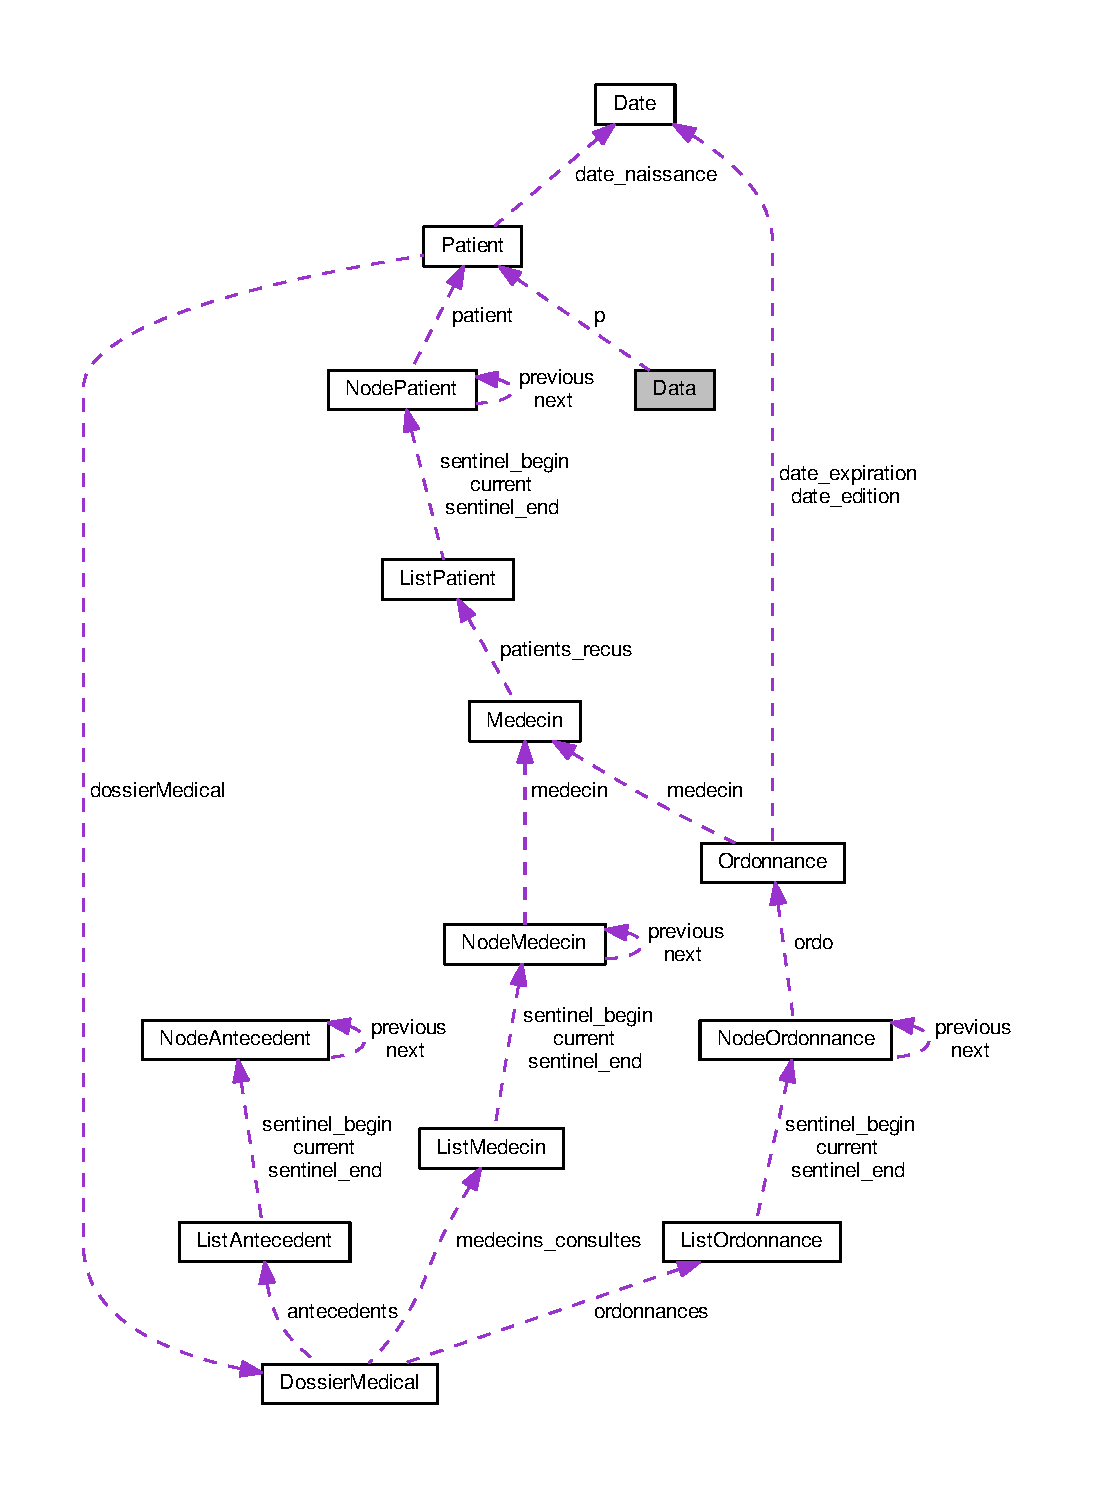
\includegraphics[width=350pt]{struct_data__coll__graph}
\end{center}
\end{figure}
\subsection*{Champs de données}
\begin{DoxyCompactItemize}
\item 
Gtk\-Widget $\ast$ \hyperlink{struct_data_ad897fb7c962d60832bc766fa99da9db9}{Enom}
\item 
Gtk\-Widget $\ast$ \hyperlink{struct_data_a7004a9a326ad19f493ca2f6f3cc4577c}{Eprenom}
\item 
Gtk\-Widget $\ast$ \hyperlink{struct_data_abd6fcac327f5f3b0629a93916e3c29da}{Enum\-Secu}
\item 
Gtk\-Widget $\ast$ \hyperlink{struct_data_ae300afceb0206bd32dc11312abd38df6}{Enum\-Tel}
\item 
Gtk\-Widget $\ast$ \hyperlink{struct_data_a1003606a7c4d6a289a7de796987f6efc}{Email}
\item 
Gtk\-Widget $\ast$ \hyperlink{struct_data_a366c31a9b090d9870030fe2ac52d6e46}{jour}
\item 
Gtk\-Widget $\ast$ \hyperlink{struct_data_a430ab7341bb11cda80f096a2ec12d8d7}{mois}
\item 
Gtk\-Widget $\ast$ \hyperlink{struct_data_a123c0853fe0470eb0a0f0af055eecc9f}{annee}
\item 
\hyperlink{struct_patient}{Patient} $\ast$ \hyperlink{struct_data_ab6da0510b3f88800fe3d3ee7e9cd9d7b}{p}
\end{DoxyCompactItemize}


\subsection{Documentation des champs}
\hypertarget{struct_data_a123c0853fe0470eb0a0f0af055eecc9f}{\index{Data@{Data}!annee@{annee}}
\index{annee@{annee}!Data@{Data}}
\subsubsection[{annee}]{\setlength{\rightskip}{0pt plus 5cm}Gtk\-Widget$\ast$ annee}}\label{struct_data_a123c0853fe0470eb0a0f0af055eecc9f}
\hypertarget{struct_data_a1003606a7c4d6a289a7de796987f6efc}{\index{Data@{Data}!Email@{Email}}
\index{Email@{Email}!Data@{Data}}
\subsubsection[{Email}]{\setlength{\rightskip}{0pt plus 5cm}Gtk\-Widget$\ast$ Email}}\label{struct_data_a1003606a7c4d6a289a7de796987f6efc}
\hypertarget{struct_data_ad897fb7c962d60832bc766fa99da9db9}{\index{Data@{Data}!Enom@{Enom}}
\index{Enom@{Enom}!Data@{Data}}
\subsubsection[{Enom}]{\setlength{\rightskip}{0pt plus 5cm}Gtk\-Widget$\ast$ Enom}}\label{struct_data_ad897fb7c962d60832bc766fa99da9db9}
\hypertarget{struct_data_abd6fcac327f5f3b0629a93916e3c29da}{\index{Data@{Data}!Enum\-Secu@{Enum\-Secu}}
\index{Enum\-Secu@{Enum\-Secu}!Data@{Data}}
\subsubsection[{Enum\-Secu}]{\setlength{\rightskip}{0pt plus 5cm}Gtk\-Widget$\ast$ Enum\-Secu}}\label{struct_data_abd6fcac327f5f3b0629a93916e3c29da}
\hypertarget{struct_data_ae300afceb0206bd32dc11312abd38df6}{\index{Data@{Data}!Enum\-Tel@{Enum\-Tel}}
\index{Enum\-Tel@{Enum\-Tel}!Data@{Data}}
\subsubsection[{Enum\-Tel}]{\setlength{\rightskip}{0pt plus 5cm}Gtk\-Widget$\ast$ Enum\-Tel}}\label{struct_data_ae300afceb0206bd32dc11312abd38df6}
\hypertarget{struct_data_a7004a9a326ad19f493ca2f6f3cc4577c}{\index{Data@{Data}!Eprenom@{Eprenom}}
\index{Eprenom@{Eprenom}!Data@{Data}}
\subsubsection[{Eprenom}]{\setlength{\rightskip}{0pt plus 5cm}Gtk\-Widget$\ast$ Eprenom}}\label{struct_data_a7004a9a326ad19f493ca2f6f3cc4577c}
\hypertarget{struct_data_a366c31a9b090d9870030fe2ac52d6e46}{\index{Data@{Data}!jour@{jour}}
\index{jour@{jour}!Data@{Data}}
\subsubsection[{jour}]{\setlength{\rightskip}{0pt plus 5cm}Gtk\-Widget$\ast$ jour}}\label{struct_data_a366c31a9b090d9870030fe2ac52d6e46}
\hypertarget{struct_data_a430ab7341bb11cda80f096a2ec12d8d7}{\index{Data@{Data}!mois@{mois}}
\index{mois@{mois}!Data@{Data}}
\subsubsection[{mois}]{\setlength{\rightskip}{0pt plus 5cm}Gtk\-Widget$\ast$ mois}}\label{struct_data_a430ab7341bb11cda80f096a2ec12d8d7}
\hypertarget{struct_data_ab6da0510b3f88800fe3d3ee7e9cd9d7b}{\index{Data@{Data}!p@{p}}
\index{p@{p}!Data@{Data}}
\subsubsection[{p}]{\setlength{\rightskip}{0pt plus 5cm}{\bf Patient}$\ast$ p}}\label{struct_data_ab6da0510b3f88800fe3d3ee7e9cd9d7b}


La documentation de cette structure a été générée à partir du fichier suivant \-:\begin{DoxyCompactItemize}
\item 
include/\-G\-P\-Calendar/\-View/\hyperlink{callbacks_8h}{callbacks.\-h}\end{DoxyCompactItemize}

\hypertarget{struct_data_r_d_v}{\section{Référence de la structure Data\-R\-D\-V}
\label{struct_data_r_d_v}\index{Data\-R\-D\-V@{Data\-R\-D\-V}}
}


{\ttfamily \#include $<$callbacks.\-h$>$}



Graphe de collaboration de Data\-R\-D\-V\-:
\nopagebreak
\begin{figure}[H]
\begin{center}
\leavevmode
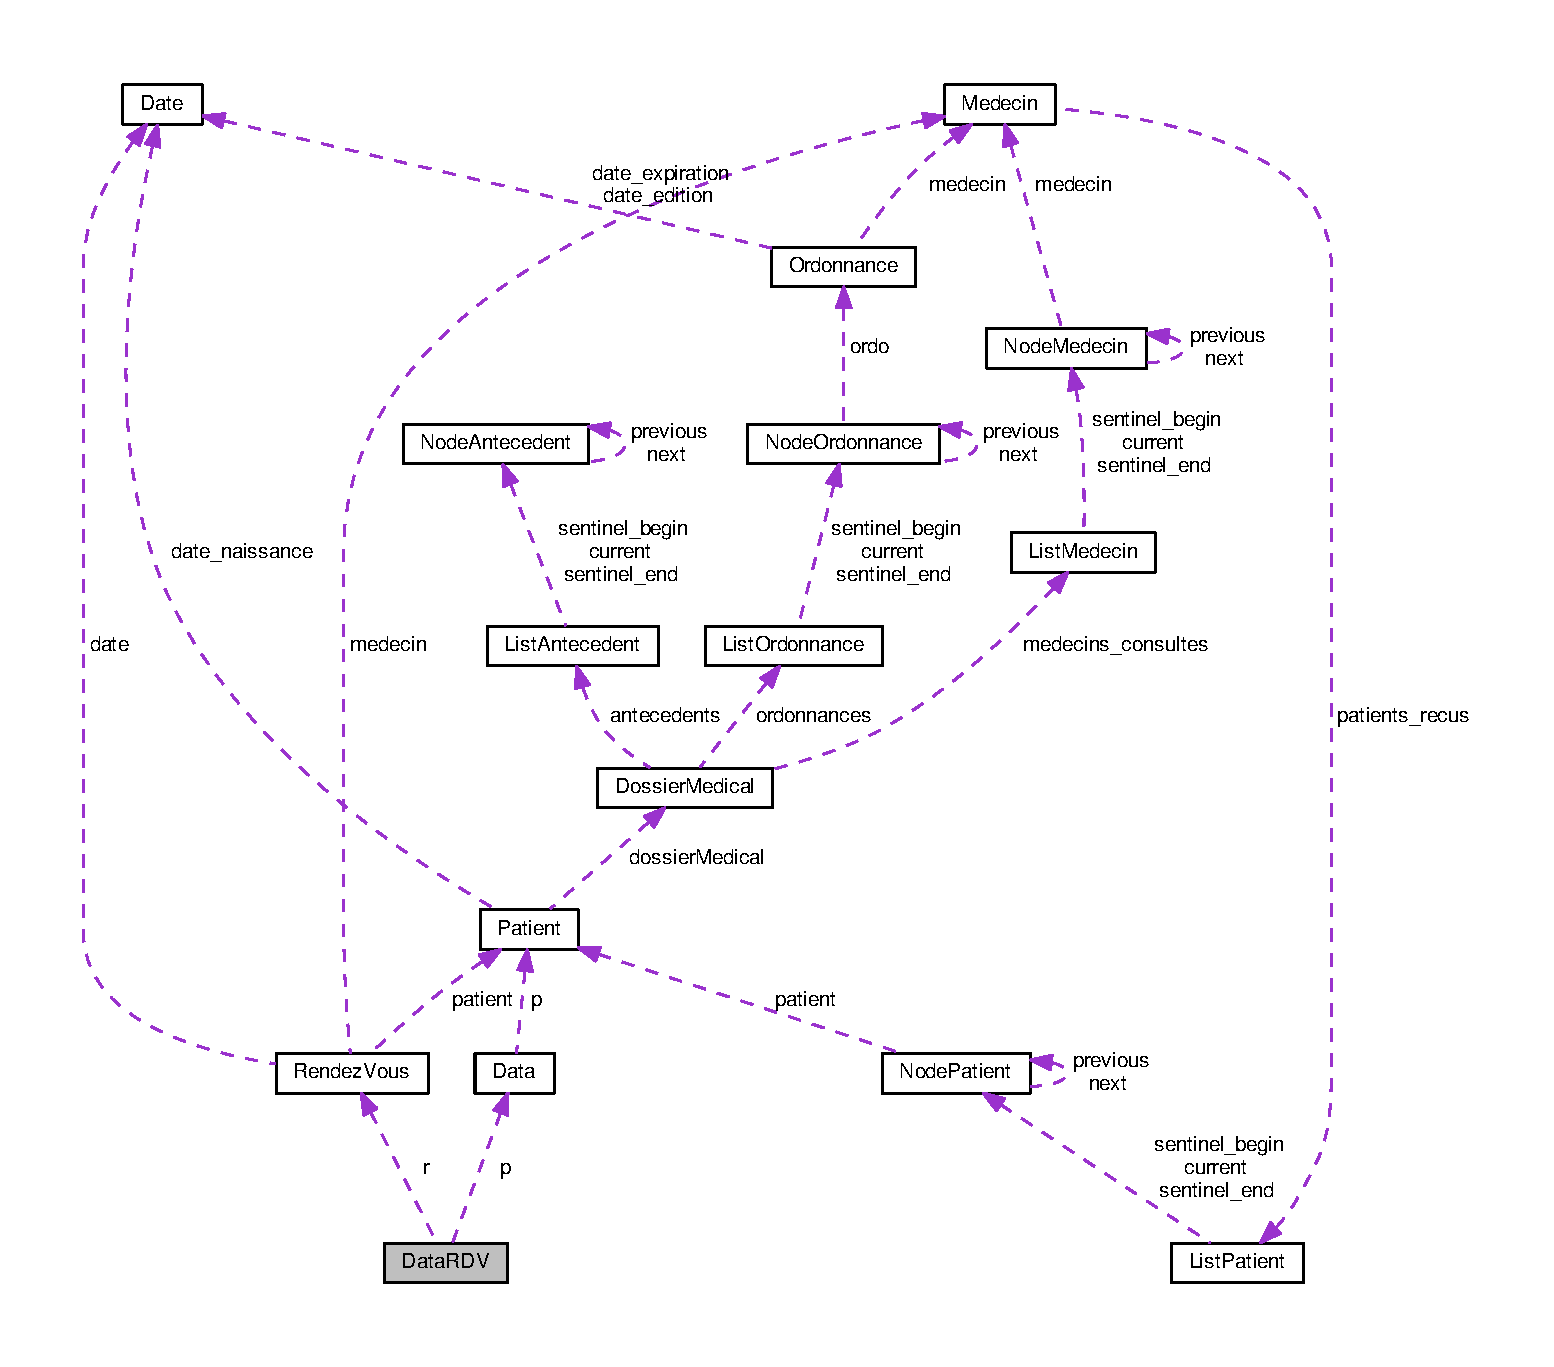
\includegraphics[width=350pt]{struct_data_r_d_v__coll__graph}
\end{center}
\end{figure}
\subsection*{Champs de données}
\begin{DoxyCompactItemize}
\item 
Gtk\-Widget $\ast$ \hyperlink{struct_data_r_d_v_a366c31a9b090d9870030fe2ac52d6e46}{jour}
\item 
Gtk\-Widget $\ast$ \hyperlink{struct_data_r_d_v_a430ab7341bb11cda80f096a2ec12d8d7}{mois}
\item 
Gtk\-Widget $\ast$ \hyperlink{struct_data_r_d_v_a123c0853fe0470eb0a0f0af055eecc9f}{annee}
\item 
Gtk\-Widget $\ast$ \hyperlink{struct_data_r_d_v_a4eb5541c2c8d07380c735d1603dc7ecb}{heure}
\item 
Gtk\-Widget $\ast$ \hyperlink{struct_data_r_d_v_a27524e2f658f644a11dbb3a8f9b5ab97}{minutes}
\item 
Gtk\-Widget $\ast$ \hyperlink{struct_data_r_d_v_a14f0b724f1decdb5bdad19079ec1d675}{duree}
\item 
Gtk\-Widget $\ast$ \hyperlink{struct_data_r_d_v_ae22ca5875ee8b6bdccaa89afda5779a4}{motif}
\item 
\hyperlink{struct_rendez_vous}{Rendez\-Vous} $\ast$ \hyperlink{struct_data_r_d_v_a017a2a103427c89eebac9921f00620ab}{r}
\item 
\hyperlink{callbacks_8h_aa29088b0ebf449924c098ffbc3fb8350}{data\-Patient} $\ast$ \hyperlink{struct_data_r_d_v_a537ec1a4e0cf2f81d81bf4da1a0a3f2f}{p}
\end{DoxyCompactItemize}


\subsection{Documentation des champs}
\hypertarget{struct_data_r_d_v_a123c0853fe0470eb0a0f0af055eecc9f}{\index{Data\-R\-D\-V@{Data\-R\-D\-V}!annee@{annee}}
\index{annee@{annee}!DataRDV@{Data\-R\-D\-V}}
\subsubsection[{annee}]{\setlength{\rightskip}{0pt plus 5cm}Gtk\-Widget$\ast$ annee}}\label{struct_data_r_d_v_a123c0853fe0470eb0a0f0af055eecc9f}
\hypertarget{struct_data_r_d_v_a14f0b724f1decdb5bdad19079ec1d675}{\index{Data\-R\-D\-V@{Data\-R\-D\-V}!duree@{duree}}
\index{duree@{duree}!DataRDV@{Data\-R\-D\-V}}
\subsubsection[{duree}]{\setlength{\rightskip}{0pt plus 5cm}Gtk\-Widget$\ast$ duree}}\label{struct_data_r_d_v_a14f0b724f1decdb5bdad19079ec1d675}
\hypertarget{struct_data_r_d_v_a4eb5541c2c8d07380c735d1603dc7ecb}{\index{Data\-R\-D\-V@{Data\-R\-D\-V}!heure@{heure}}
\index{heure@{heure}!DataRDV@{Data\-R\-D\-V}}
\subsubsection[{heure}]{\setlength{\rightskip}{0pt plus 5cm}Gtk\-Widget$\ast$ heure}}\label{struct_data_r_d_v_a4eb5541c2c8d07380c735d1603dc7ecb}
\hypertarget{struct_data_r_d_v_a366c31a9b090d9870030fe2ac52d6e46}{\index{Data\-R\-D\-V@{Data\-R\-D\-V}!jour@{jour}}
\index{jour@{jour}!DataRDV@{Data\-R\-D\-V}}
\subsubsection[{jour}]{\setlength{\rightskip}{0pt plus 5cm}Gtk\-Widget$\ast$ jour}}\label{struct_data_r_d_v_a366c31a9b090d9870030fe2ac52d6e46}
\hypertarget{struct_data_r_d_v_a27524e2f658f644a11dbb3a8f9b5ab97}{\index{Data\-R\-D\-V@{Data\-R\-D\-V}!minutes@{minutes}}
\index{minutes@{minutes}!DataRDV@{Data\-R\-D\-V}}
\subsubsection[{minutes}]{\setlength{\rightskip}{0pt plus 5cm}Gtk\-Widget$\ast$ minutes}}\label{struct_data_r_d_v_a27524e2f658f644a11dbb3a8f9b5ab97}
\hypertarget{struct_data_r_d_v_a430ab7341bb11cda80f096a2ec12d8d7}{\index{Data\-R\-D\-V@{Data\-R\-D\-V}!mois@{mois}}
\index{mois@{mois}!DataRDV@{Data\-R\-D\-V}}
\subsubsection[{mois}]{\setlength{\rightskip}{0pt plus 5cm}Gtk\-Widget$\ast$ mois}}\label{struct_data_r_d_v_a430ab7341bb11cda80f096a2ec12d8d7}
\hypertarget{struct_data_r_d_v_ae22ca5875ee8b6bdccaa89afda5779a4}{\index{Data\-R\-D\-V@{Data\-R\-D\-V}!motif@{motif}}
\index{motif@{motif}!DataRDV@{Data\-R\-D\-V}}
\subsubsection[{motif}]{\setlength{\rightskip}{0pt plus 5cm}Gtk\-Widget$\ast$ motif}}\label{struct_data_r_d_v_ae22ca5875ee8b6bdccaa89afda5779a4}
\hypertarget{struct_data_r_d_v_a537ec1a4e0cf2f81d81bf4da1a0a3f2f}{\index{Data\-R\-D\-V@{Data\-R\-D\-V}!p@{p}}
\index{p@{p}!DataRDV@{Data\-R\-D\-V}}
\subsubsection[{p}]{\setlength{\rightskip}{0pt plus 5cm}{\bf data\-Patient}$\ast$ p}}\label{struct_data_r_d_v_a537ec1a4e0cf2f81d81bf4da1a0a3f2f}
\hypertarget{struct_data_r_d_v_a017a2a103427c89eebac9921f00620ab}{\index{Data\-R\-D\-V@{Data\-R\-D\-V}!r@{r}}
\index{r@{r}!DataRDV@{Data\-R\-D\-V}}
\subsubsection[{r}]{\setlength{\rightskip}{0pt plus 5cm}{\bf Rendez\-Vous}$\ast$ r}}\label{struct_data_r_d_v_a017a2a103427c89eebac9921f00620ab}


La documentation de cette structure a été générée à partir du fichier suivant \-:\begin{DoxyCompactItemize}
\item 
include/\-G\-P\-Calendar/\-View/\hyperlink{callbacks_8h}{callbacks.\-h}\end{DoxyCompactItemize}

\hypertarget{struct_date}{\section{Référence de la structure Date}
\label{struct_date}\index{Date@{Date}}
}


{\ttfamily \#include $<$date.\-h$>$}

\subsection*{Champs de données}
\begin{DoxyCompactItemize}
\item 
int \hyperlink{struct_date_acfe2ff64f5396827db36f1575c5e99d8}{annee}
\item 
int \hyperlink{struct_date_af4d47133f30c1a134b6cecf5cedd7db9}{mois}
\item 
int \hyperlink{struct_date_aec8e61b4e27d935e47eba0485425da38}{jour}
\end{DoxyCompactItemize}


\subsection{Documentation des champs}
\hypertarget{struct_date_acfe2ff64f5396827db36f1575c5e99d8}{\index{Date@{Date}!annee@{annee}}
\index{annee@{annee}!Date@{Date}}
\subsubsection[{annee}]{\setlength{\rightskip}{0pt plus 5cm}int annee}}\label{struct_date_acfe2ff64f5396827db36f1575c5e99d8}
\hypertarget{struct_date_aec8e61b4e27d935e47eba0485425da38}{\index{Date@{Date}!jour@{jour}}
\index{jour@{jour}!Date@{Date}}
\subsubsection[{jour}]{\setlength{\rightskip}{0pt plus 5cm}int jour}}\label{struct_date_aec8e61b4e27d935e47eba0485425da38}
\hypertarget{struct_date_af4d47133f30c1a134b6cecf5cedd7db9}{\index{Date@{Date}!mois@{mois}}
\index{mois@{mois}!Date@{Date}}
\subsubsection[{mois}]{\setlength{\rightskip}{0pt plus 5cm}int mois}}\label{struct_date_af4d47133f30c1a134b6cecf5cedd7db9}


La documentation de cette structure a été générée à partir du fichier suivant \-:\begin{DoxyCompactItemize}
\item 
include/\-G\-P\-Calendar/\-Model/\hyperlink{date_8h}{date.\-h}\end{DoxyCompactItemize}

\hypertarget{struct_dossier_medical}{\section{Référence de la structure Dossier\-Medical}
\label{struct_dossier_medical}\index{Dossier\-Medical@{Dossier\-Medical}}
}


{\ttfamily \#include $<$dossier\-\_\-medical.\-h$>$}



Graphe de collaboration de Dossier\-Medical\-:
\nopagebreak
\begin{figure}[H]
\begin{center}
\leavevmode
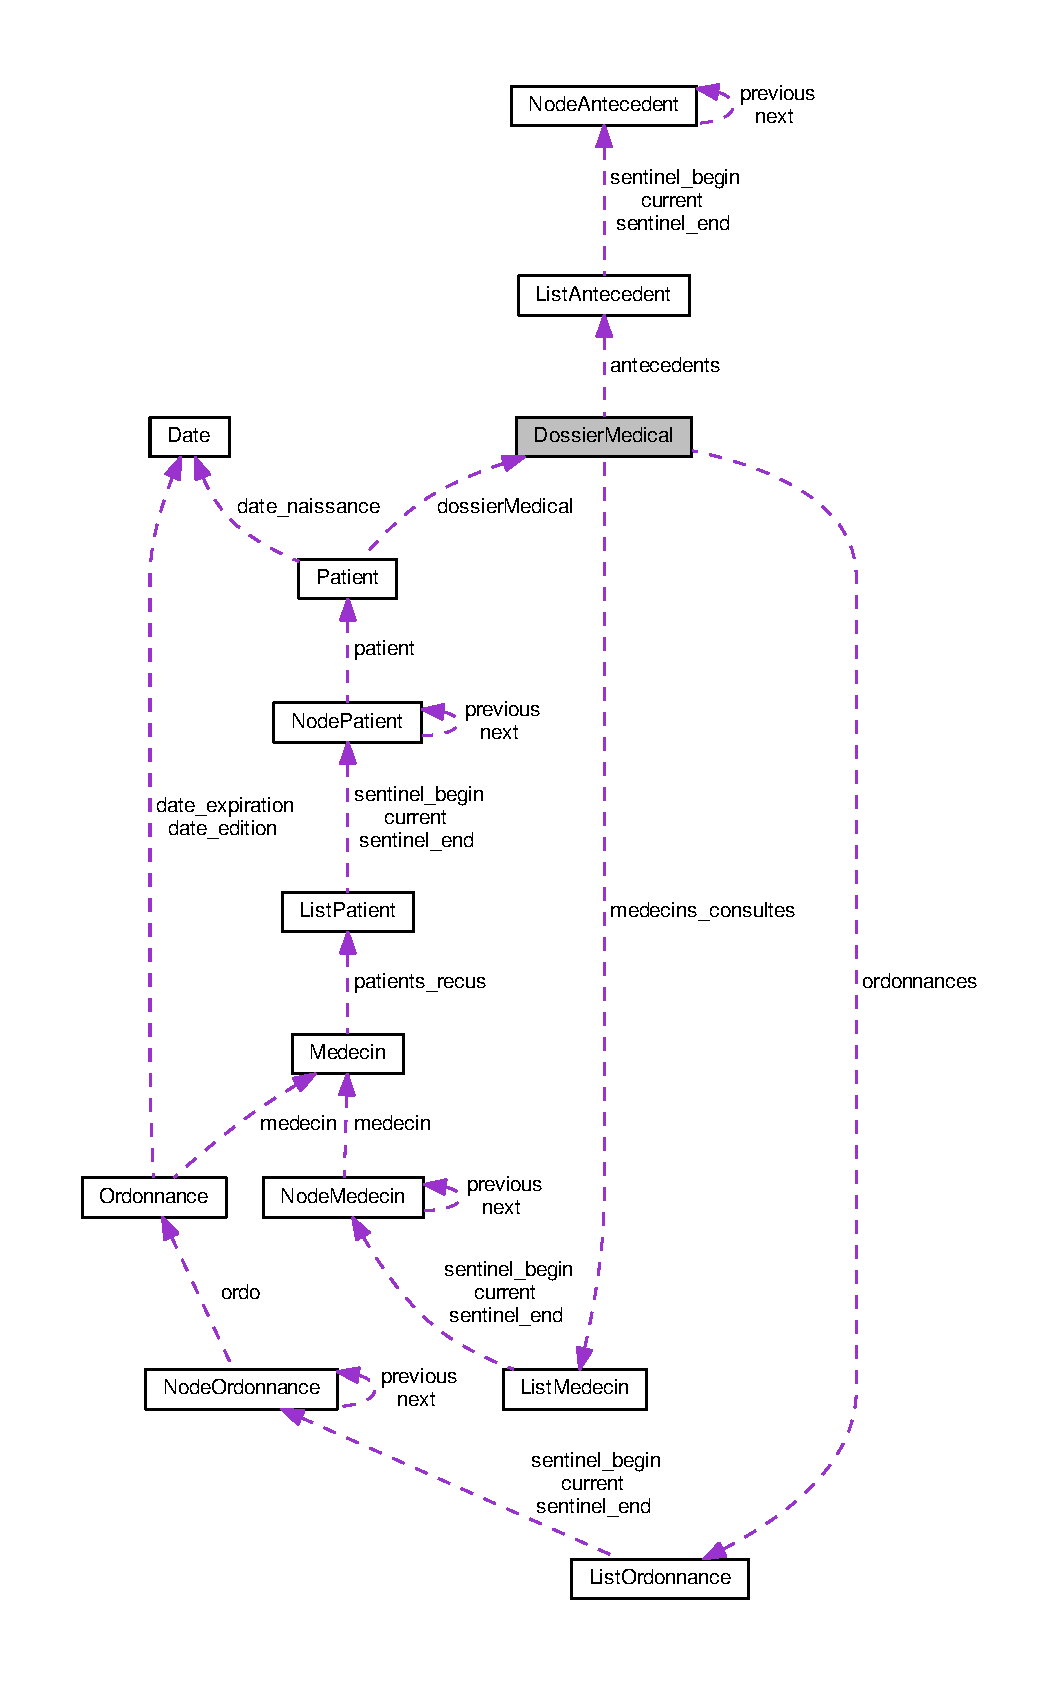
\includegraphics[height=550pt]{struct_dossier_medical__coll__graph}
\end{center}
\end{figure}
\subsection*{Champs de données}
\begin{DoxyCompactItemize}
\item 
\hyperlink{struct_list_medecin}{List\-Medecin} $\ast$ \hyperlink{struct_dossier_medical_a7f90f000e882b02f6ce24bbef6ce32f0}{medecins\-\_\-consultes}
\item 
\hyperlink{struct_list_ordonnance}{List\-Ordonnance} $\ast$ \hyperlink{struct_dossier_medical_ac4e1845527931ccc76c5ab1c1241d0e1}{ordonnances}
\item 
\hyperlink{struct_list_antecedent}{List\-Antecedent} $\ast$ \hyperlink{struct_dossier_medical_a63a3ed7e25a889fb251e7de019a7d63c}{antecedents}
\end{DoxyCompactItemize}


\subsection{Documentation des champs}
\hypertarget{struct_dossier_medical_a63a3ed7e25a889fb251e7de019a7d63c}{\index{Dossier\-Medical@{Dossier\-Medical}!antecedents@{antecedents}}
\index{antecedents@{antecedents}!DossierMedical@{Dossier\-Medical}}
\subsubsection[{antecedents}]{\setlength{\rightskip}{0pt plus 5cm}{\bf List\-Antecedent}$\ast$ antecedents}}\label{struct_dossier_medical_a63a3ed7e25a889fb251e7de019a7d63c}
Pas d'antécédents pour l'instant (pas implémenté dans dossier médical.\-c et dans Json.\-c \hypertarget{struct_dossier_medical_a7f90f000e882b02f6ce24bbef6ce32f0}{\index{Dossier\-Medical@{Dossier\-Medical}!medecins\-\_\-consultes@{medecins\-\_\-consultes}}
\index{medecins\-\_\-consultes@{medecins\-\_\-consultes}!DossierMedical@{Dossier\-Medical}}
\subsubsection[{medecins\-\_\-consultes}]{\setlength{\rightskip}{0pt plus 5cm}{\bf List\-Medecin}$\ast$ medecins\-\_\-consultes}}\label{struct_dossier_medical_a7f90f000e882b02f6ce24bbef6ce32f0}
\hypertarget{struct_dossier_medical_ac4e1845527931ccc76c5ab1c1241d0e1}{\index{Dossier\-Medical@{Dossier\-Medical}!ordonnances@{ordonnances}}
\index{ordonnances@{ordonnances}!DossierMedical@{Dossier\-Medical}}
\subsubsection[{ordonnances}]{\setlength{\rightskip}{0pt plus 5cm}{\bf List\-Ordonnance}$\ast$ ordonnances}}\label{struct_dossier_medical_ac4e1845527931ccc76c5ab1c1241d0e1}


La documentation de cette structure a été générée à partir du fichier suivant \-:\begin{DoxyCompactItemize}
\item 
include/\-G\-P\-Calendar/\-Model/\hyperlink{dossier__medical_8h}{dossier\-\_\-medical.\-h}\end{DoxyCompactItemize}

\hypertarget{struct_list_annee}{\section{Référence de la structure List\-Annee}
\label{struct_list_annee}\index{List\-Annee@{List\-Annee}}
}


{\ttfamily \#include $<$calendrier.\-h$>$}



Graphe de collaboration de List\-Annee\-:
\nopagebreak
\begin{figure}[H]
\begin{center}
\leavevmode
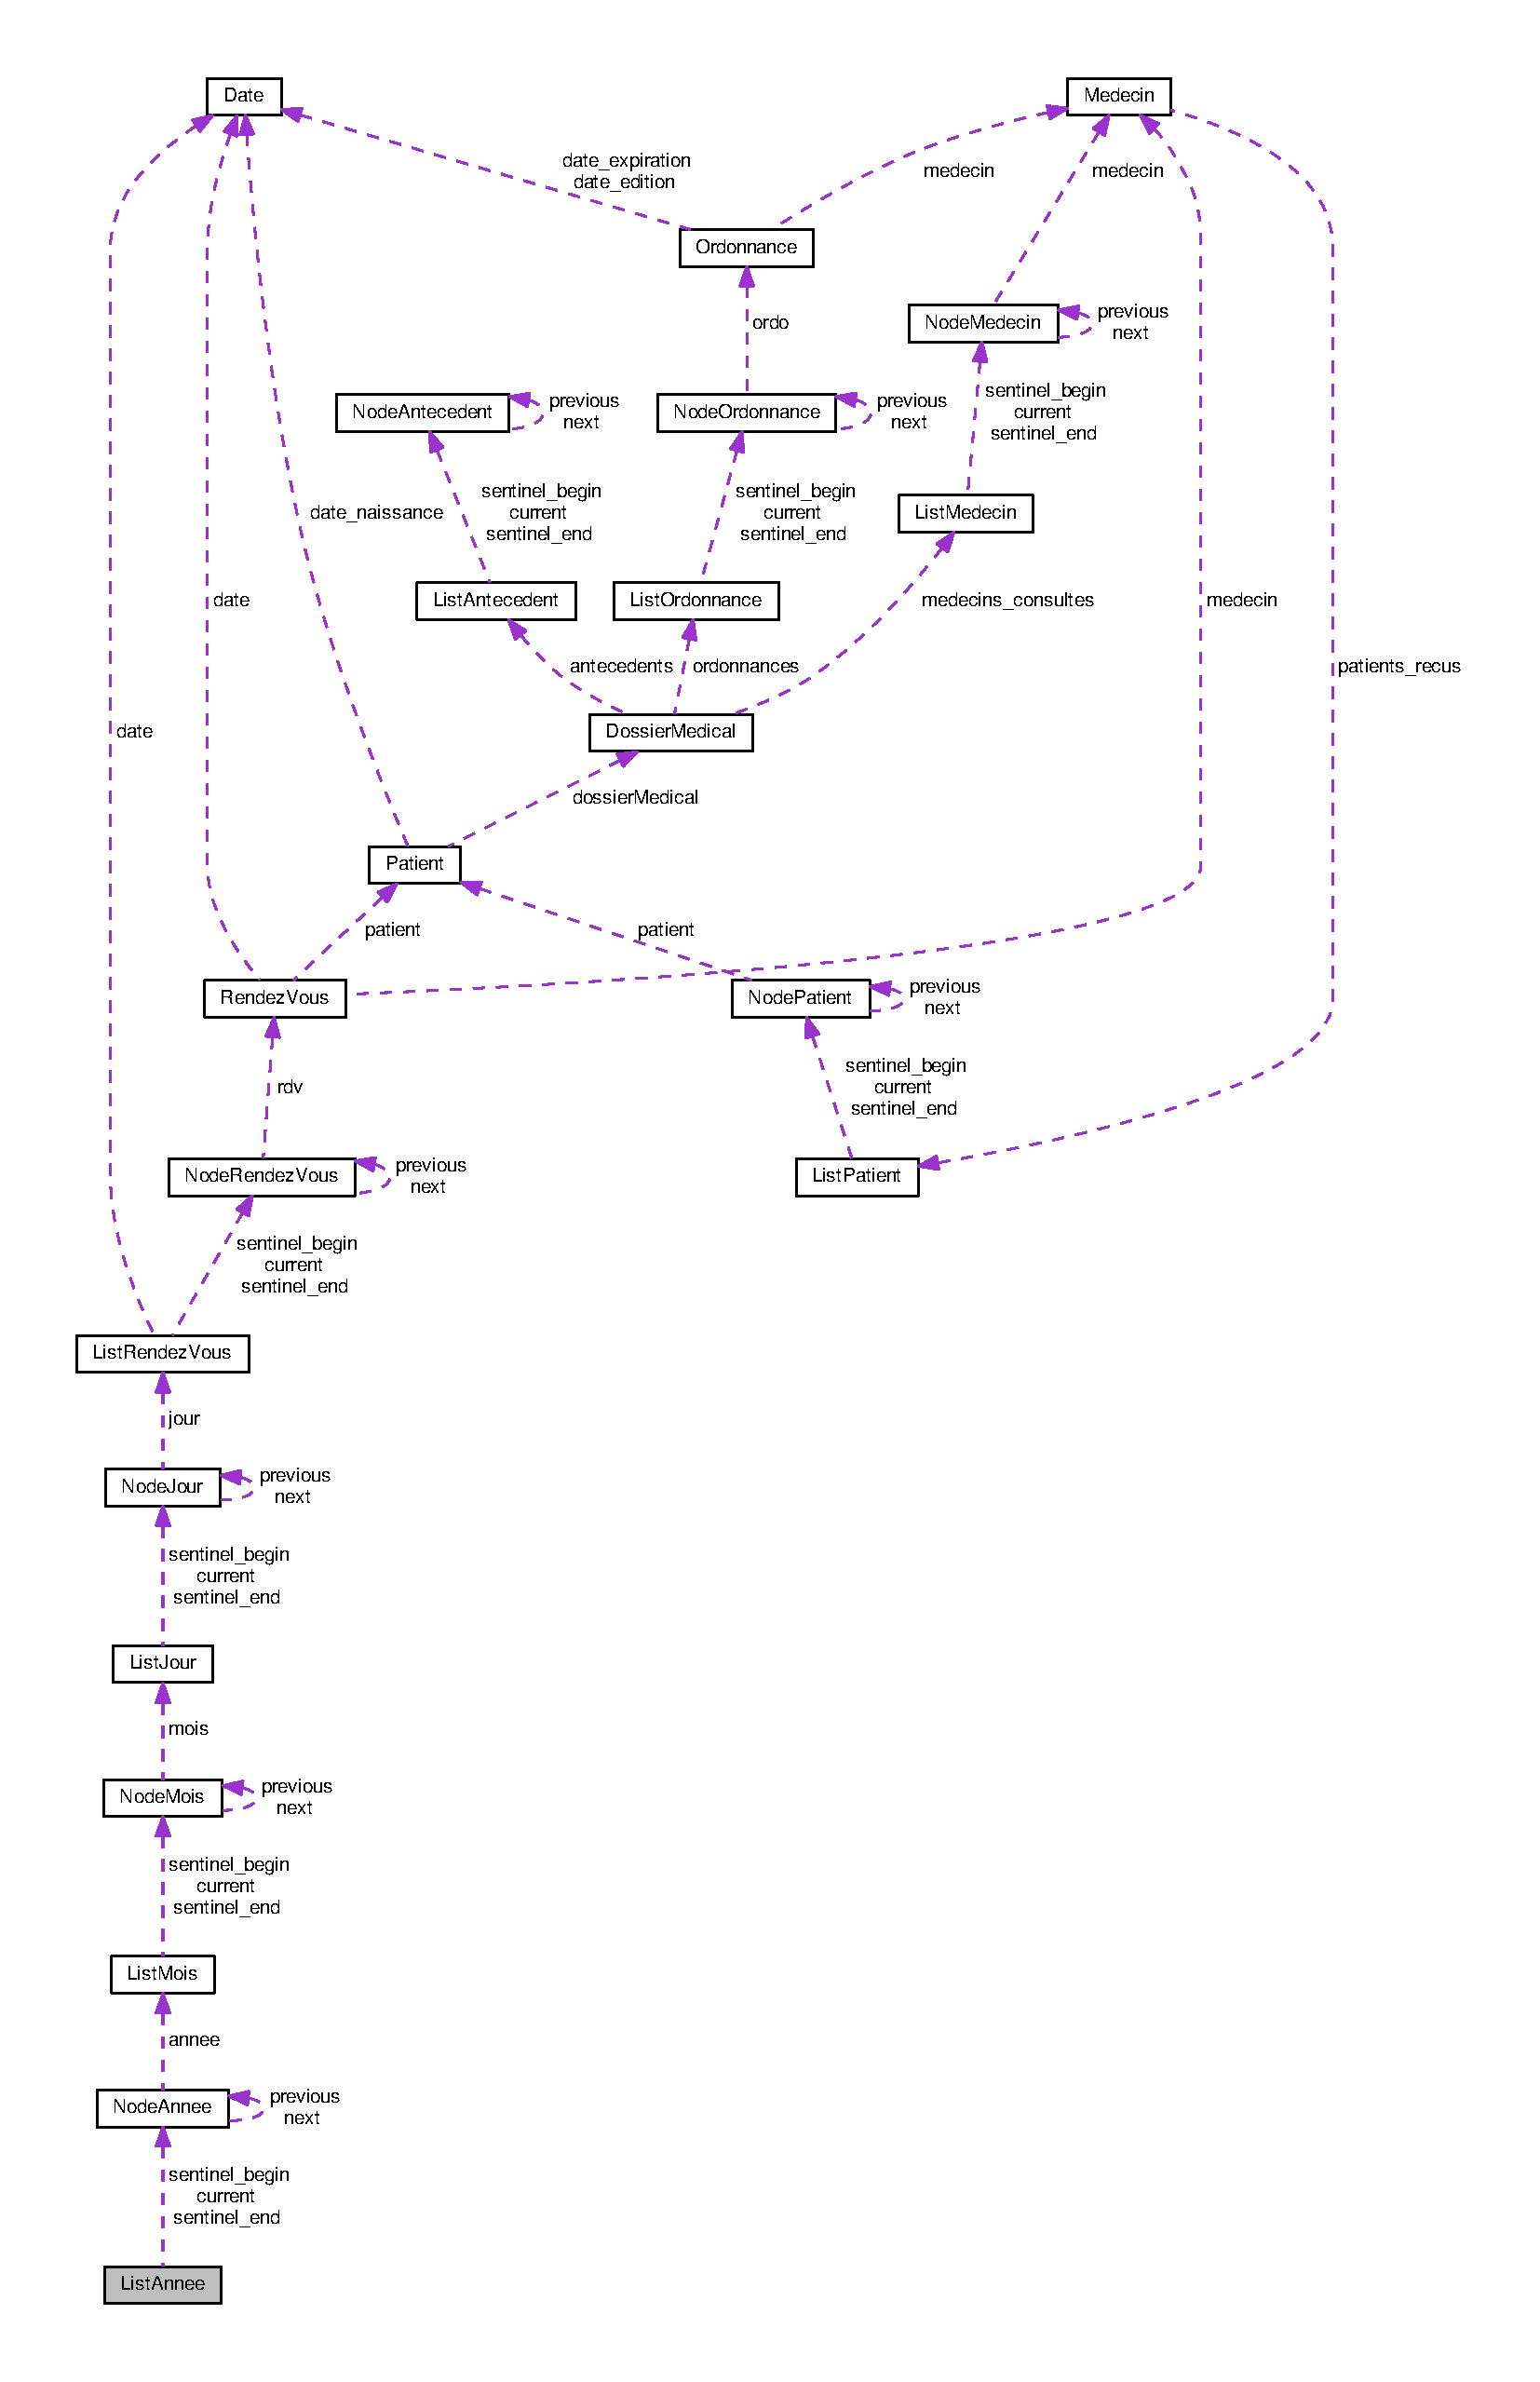
\includegraphics[width=350pt]{struct_list_annee__coll__graph}
\end{center}
\end{figure}
\subsection*{Champs de données}
\begin{DoxyCompactItemize}
\item 
\hyperlink{struct_node_annee}{Node\-Annee} \hyperlink{struct_list_annee_a8e3c43a4e3e1420a9a6054eea884106e}{sentinel\-\_\-begin}
\item 
\hyperlink{struct_node_annee}{Node\-Annee} $\ast$ \hyperlink{struct_list_annee_a5f39192750953f444d3b63dea208efb4}{current}
\item 
\hyperlink{struct_node_annee}{Node\-Annee} \hyperlink{struct_list_annee_a402cfcc871ccc44cf40bc211273987d8}{sentinel\-\_\-end}
\end{DoxyCompactItemize}


\subsection{Documentation des champs}
\hypertarget{struct_list_annee_a5f39192750953f444d3b63dea208efb4}{\index{List\-Annee@{List\-Annee}!current@{current}}
\index{current@{current}!ListAnnee@{List\-Annee}}
\subsubsection[{current}]{\setlength{\rightskip}{0pt plus 5cm}{\bf Node\-Annee}$\ast$ current}}\label{struct_list_annee_a5f39192750953f444d3b63dea208efb4}
\hypertarget{struct_list_annee_a8e3c43a4e3e1420a9a6054eea884106e}{\index{List\-Annee@{List\-Annee}!sentinel\-\_\-begin@{sentinel\-\_\-begin}}
\index{sentinel\-\_\-begin@{sentinel\-\_\-begin}!ListAnnee@{List\-Annee}}
\subsubsection[{sentinel\-\_\-begin}]{\setlength{\rightskip}{0pt plus 5cm}{\bf Node\-Annee} sentinel\-\_\-begin}}\label{struct_list_annee_a8e3c43a4e3e1420a9a6054eea884106e}
\hypertarget{struct_list_annee_a402cfcc871ccc44cf40bc211273987d8}{\index{List\-Annee@{List\-Annee}!sentinel\-\_\-end@{sentinel\-\_\-end}}
\index{sentinel\-\_\-end@{sentinel\-\_\-end}!ListAnnee@{List\-Annee}}
\subsubsection[{sentinel\-\_\-end}]{\setlength{\rightskip}{0pt plus 5cm}{\bf Node\-Annee} sentinel\-\_\-end}}\label{struct_list_annee_a402cfcc871ccc44cf40bc211273987d8}


La documentation de cette structure a été générée à partir du fichier suivant \-:\begin{DoxyCompactItemize}
\item 
include/\-G\-P\-Calendar/\-Model/\hyperlink{calendrier_8h}{calendrier.\-h}\end{DoxyCompactItemize}

\hypertarget{struct_list_antecedent}{\section{Référence de la structure List\-Antecedent}
\label{struct_list_antecedent}\index{List\-Antecedent@{List\-Antecedent}}
}


{\ttfamily \#include $<$dossier\-\_\-medical.\-h$>$}



Graphe de collaboration de List\-Antecedent\-:
\nopagebreak
\begin{figure}[H]
\begin{center}
\leavevmode
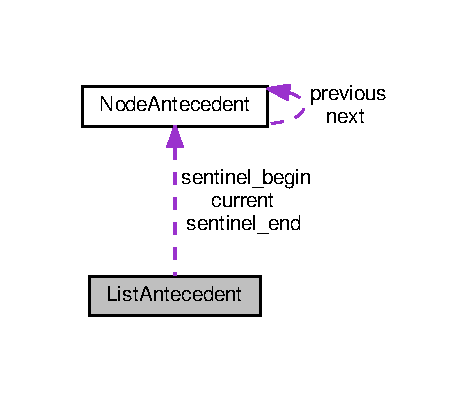
\includegraphics[width=226pt]{struct_list_antecedent__coll__graph}
\end{center}
\end{figure}
\subsection*{Champs de données}
\begin{DoxyCompactItemize}
\item 
\hyperlink{struct_node_antecedent}{Node\-Antecedent} \hyperlink{struct_list_antecedent_a2aa9bf6f515609f5be242be5c329e78b}{sentinel\-\_\-begin}
\item 
\hyperlink{struct_node_antecedent}{Node\-Antecedent} $\ast$ \hyperlink{struct_list_antecedent_a93d09acaf5d014c14988d6a2b03cb6c3}{current}
\item 
\hyperlink{struct_node_antecedent}{Node\-Antecedent} \hyperlink{struct_list_antecedent_a7f9cde4039bce42b1cdf76bb41731bb4}{sentinel\-\_\-end}
\end{DoxyCompactItemize}


\subsection{Documentation des champs}
\hypertarget{struct_list_antecedent_a93d09acaf5d014c14988d6a2b03cb6c3}{\index{List\-Antecedent@{List\-Antecedent}!current@{current}}
\index{current@{current}!ListAntecedent@{List\-Antecedent}}
\subsubsection[{current}]{\setlength{\rightskip}{0pt plus 5cm}{\bf Node\-Antecedent}$\ast$ current}}\label{struct_list_antecedent_a93d09acaf5d014c14988d6a2b03cb6c3}
\hypertarget{struct_list_antecedent_a2aa9bf6f515609f5be242be5c329e78b}{\index{List\-Antecedent@{List\-Antecedent}!sentinel\-\_\-begin@{sentinel\-\_\-begin}}
\index{sentinel\-\_\-begin@{sentinel\-\_\-begin}!ListAntecedent@{List\-Antecedent}}
\subsubsection[{sentinel\-\_\-begin}]{\setlength{\rightskip}{0pt plus 5cm}{\bf Node\-Antecedent} sentinel\-\_\-begin}}\label{struct_list_antecedent_a2aa9bf6f515609f5be242be5c329e78b}
\hypertarget{struct_list_antecedent_a7f9cde4039bce42b1cdf76bb41731bb4}{\index{List\-Antecedent@{List\-Antecedent}!sentinel\-\_\-end@{sentinel\-\_\-end}}
\index{sentinel\-\_\-end@{sentinel\-\_\-end}!ListAntecedent@{List\-Antecedent}}
\subsubsection[{sentinel\-\_\-end}]{\setlength{\rightskip}{0pt plus 5cm}{\bf Node\-Antecedent} sentinel\-\_\-end}}\label{struct_list_antecedent_a7f9cde4039bce42b1cdf76bb41731bb4}


La documentation de cette structure a été générée à partir du fichier suivant \-:\begin{DoxyCompactItemize}
\item 
include/\-G\-P\-Calendar/\-Model/\hyperlink{dossier__medical_8h}{dossier\-\_\-medical.\-h}\end{DoxyCompactItemize}

\hypertarget{struct_list_jour}{\section{Référence de la structure List\-Jour}
\label{struct_list_jour}\index{List\-Jour@{List\-Jour}}
}


{\ttfamily \#include $<$calendrier.\-h$>$}



Graphe de collaboration de List\-Jour\-:
\nopagebreak
\begin{figure}[H]
\begin{center}
\leavevmode
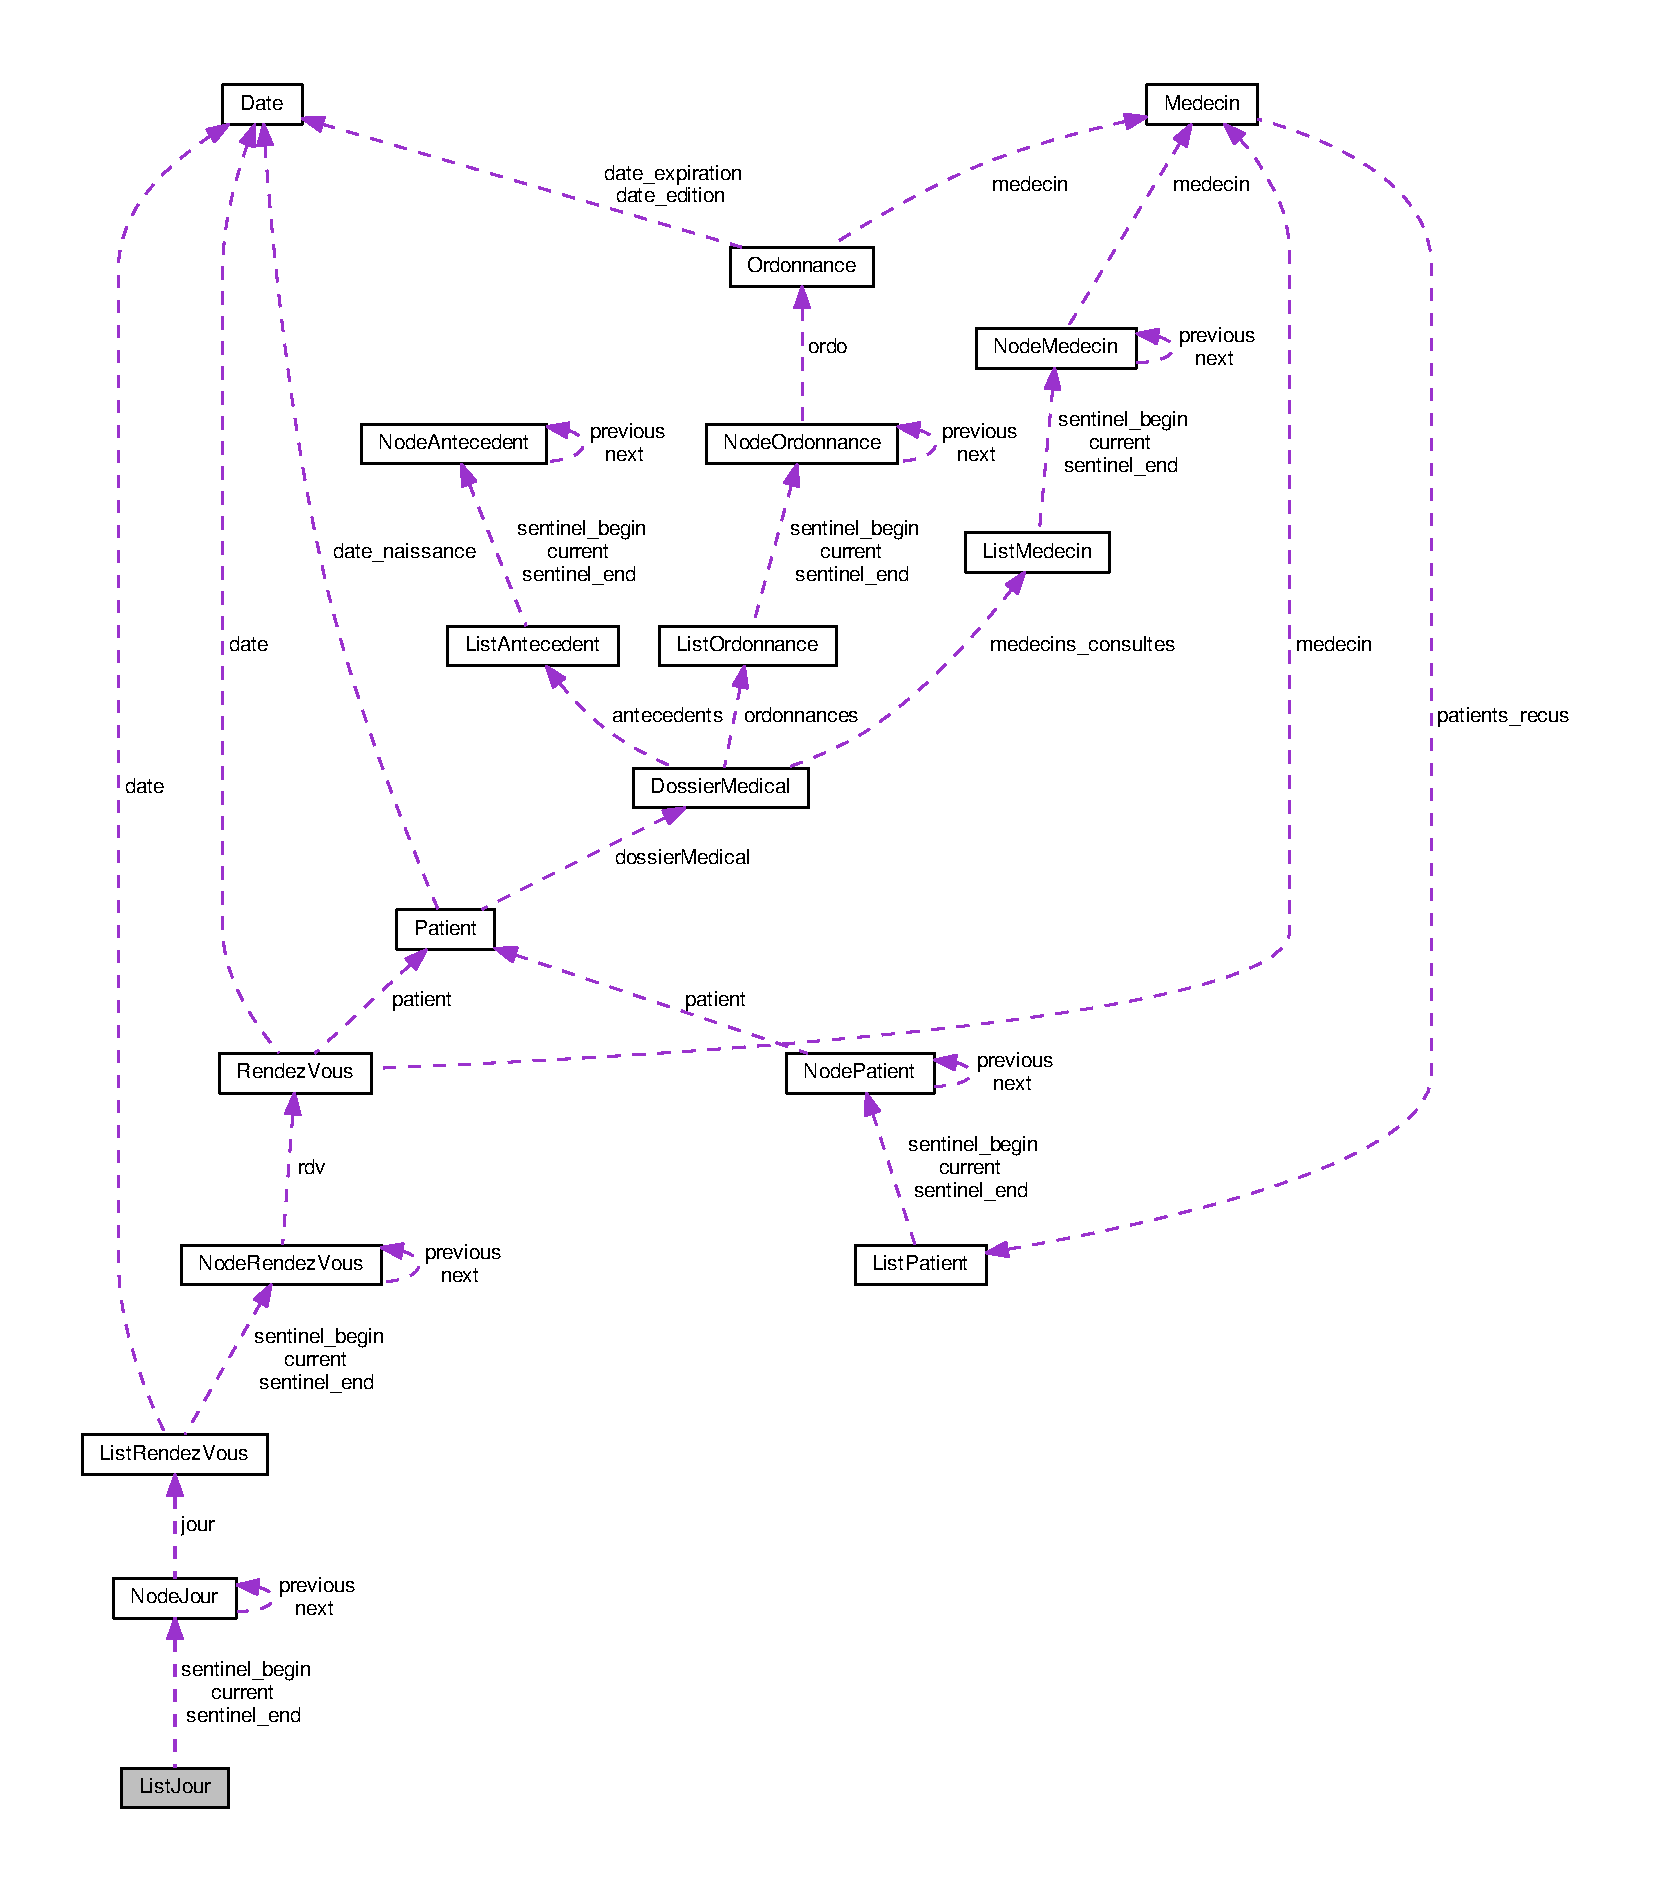
\includegraphics[width=350pt]{struct_list_jour__coll__graph}
\end{center}
\end{figure}
\subsection*{Champs de données}
\begin{DoxyCompactItemize}
\item 
int \hyperlink{struct_list_jour_af4d47133f30c1a134b6cecf5cedd7db9}{mois}
\item 
\hyperlink{struct_node_jour}{Node\-Jour} \hyperlink{struct_list_jour_ae0b0389d82fac1c68ddbb3a3cdcbd194}{sentinel\-\_\-begin}
\item 
\hyperlink{struct_node_jour}{Node\-Jour} $\ast$ \hyperlink{struct_list_jour_ac67b6c04656e03ceefbfd375d8f63a9e}{current}
\item 
\hyperlink{struct_node_jour}{Node\-Jour} \hyperlink{struct_list_jour_a0d872681cde96effd5a33a06062ceffd}{sentinel\-\_\-end}
\end{DoxyCompactItemize}


\subsection{Documentation des champs}
\hypertarget{struct_list_jour_ac67b6c04656e03ceefbfd375d8f63a9e}{\index{List\-Jour@{List\-Jour}!current@{current}}
\index{current@{current}!ListJour@{List\-Jour}}
\subsubsection[{current}]{\setlength{\rightskip}{0pt plus 5cm}{\bf Node\-Jour}$\ast$ current}}\label{struct_list_jour_ac67b6c04656e03ceefbfd375d8f63a9e}
\hypertarget{struct_list_jour_af4d47133f30c1a134b6cecf5cedd7db9}{\index{List\-Jour@{List\-Jour}!mois@{mois}}
\index{mois@{mois}!ListJour@{List\-Jour}}
\subsubsection[{mois}]{\setlength{\rightskip}{0pt plus 5cm}int mois}}\label{struct_list_jour_af4d47133f30c1a134b6cecf5cedd7db9}
\hypertarget{struct_list_jour_ae0b0389d82fac1c68ddbb3a3cdcbd194}{\index{List\-Jour@{List\-Jour}!sentinel\-\_\-begin@{sentinel\-\_\-begin}}
\index{sentinel\-\_\-begin@{sentinel\-\_\-begin}!ListJour@{List\-Jour}}
\subsubsection[{sentinel\-\_\-begin}]{\setlength{\rightskip}{0pt plus 5cm}{\bf Node\-Jour} sentinel\-\_\-begin}}\label{struct_list_jour_ae0b0389d82fac1c68ddbb3a3cdcbd194}
\hypertarget{struct_list_jour_a0d872681cde96effd5a33a06062ceffd}{\index{List\-Jour@{List\-Jour}!sentinel\-\_\-end@{sentinel\-\_\-end}}
\index{sentinel\-\_\-end@{sentinel\-\_\-end}!ListJour@{List\-Jour}}
\subsubsection[{sentinel\-\_\-end}]{\setlength{\rightskip}{0pt plus 5cm}{\bf Node\-Jour} sentinel\-\_\-end}}\label{struct_list_jour_a0d872681cde96effd5a33a06062ceffd}


La documentation de cette structure a été générée à partir du fichier suivant \-:\begin{DoxyCompactItemize}
\item 
include/\-G\-P\-Calendar/\-Model/\hyperlink{calendrier_8h}{calendrier.\-h}\end{DoxyCompactItemize}

\hypertarget{struct_list_medecin}{\section{Référence de la structure List\-Medecin}
\label{struct_list_medecin}\index{List\-Medecin@{List\-Medecin}}
}


{\ttfamily \#include $<$medecin.\-h$>$}



Graphe de collaboration de List\-Medecin\-:
\nopagebreak
\begin{figure}[H]
\begin{center}
\leavevmode
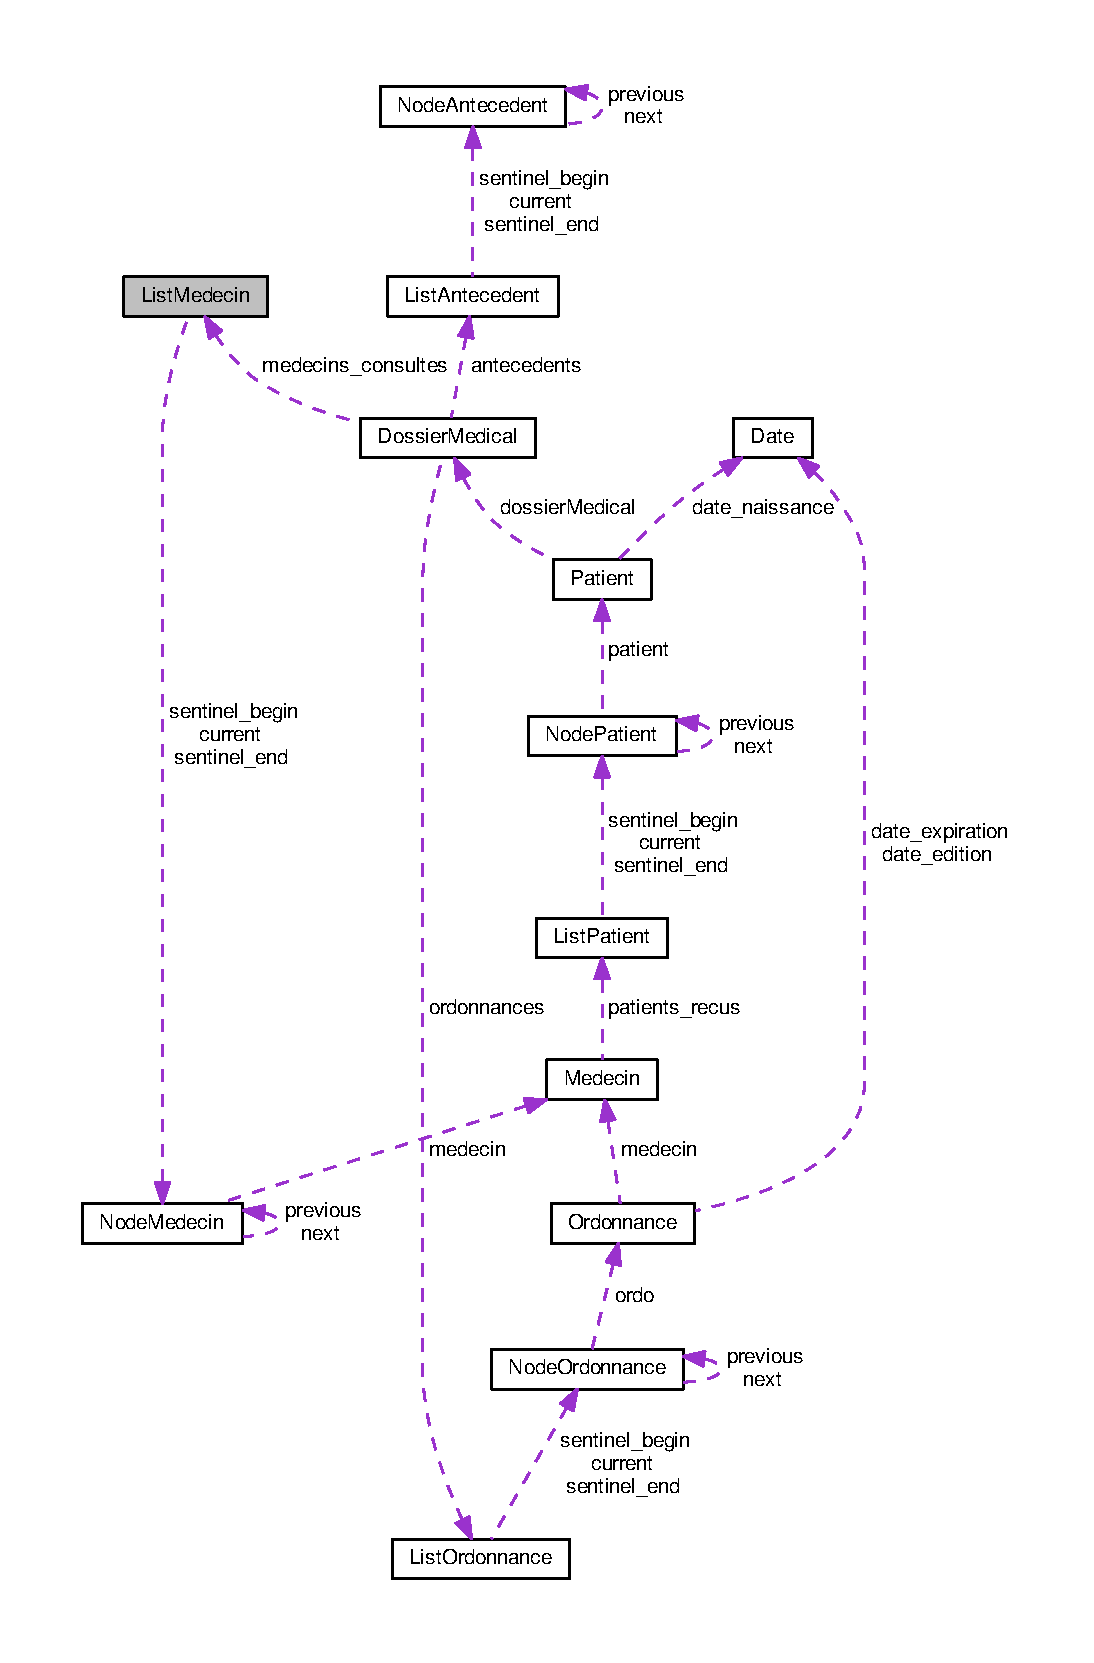
\includegraphics[width=350pt]{struct_list_medecin__coll__graph}
\end{center}
\end{figure}
\subsection*{Champs de données}
\begin{DoxyCompactItemize}
\item 
\hyperlink{struct_node_medecin}{Node\-Medecin} \hyperlink{struct_list_medecin_a1bbeb88d0dd5cfca362bc969a3771420}{sentinel\-\_\-begin}
\item 
\hyperlink{struct_node_medecin}{Node\-Medecin} $\ast$ \hyperlink{struct_list_medecin_a8da16810fc962b178bf6e06873609e0f}{current}
\item 
\hyperlink{struct_node_medecin}{Node\-Medecin} \hyperlink{struct_list_medecin_af3ae3b9febe4f1a4962f472064f963b6}{sentinel\-\_\-end}
\end{DoxyCompactItemize}


\subsection{Documentation des champs}
\hypertarget{struct_list_medecin_a8da16810fc962b178bf6e06873609e0f}{\index{List\-Medecin@{List\-Medecin}!current@{current}}
\index{current@{current}!ListMedecin@{List\-Medecin}}
\subsubsection[{current}]{\setlength{\rightskip}{0pt plus 5cm}{\bf Node\-Medecin}$\ast$ current}}\label{struct_list_medecin_a8da16810fc962b178bf6e06873609e0f}
\hypertarget{struct_list_medecin_a1bbeb88d0dd5cfca362bc969a3771420}{\index{List\-Medecin@{List\-Medecin}!sentinel\-\_\-begin@{sentinel\-\_\-begin}}
\index{sentinel\-\_\-begin@{sentinel\-\_\-begin}!ListMedecin@{List\-Medecin}}
\subsubsection[{sentinel\-\_\-begin}]{\setlength{\rightskip}{0pt plus 5cm}{\bf Node\-Medecin} sentinel\-\_\-begin}}\label{struct_list_medecin_a1bbeb88d0dd5cfca362bc969a3771420}
\hypertarget{struct_list_medecin_af3ae3b9febe4f1a4962f472064f963b6}{\index{List\-Medecin@{List\-Medecin}!sentinel\-\_\-end@{sentinel\-\_\-end}}
\index{sentinel\-\_\-end@{sentinel\-\_\-end}!ListMedecin@{List\-Medecin}}
\subsubsection[{sentinel\-\_\-end}]{\setlength{\rightskip}{0pt plus 5cm}{\bf Node\-Medecin} sentinel\-\_\-end}}\label{struct_list_medecin_af3ae3b9febe4f1a4962f472064f963b6}


La documentation de cette structure a été générée à partir du fichier suivant \-:\begin{DoxyCompactItemize}
\item 
include/\-G\-P\-Calendar/\-Model/\hyperlink{medecin_8h}{medecin.\-h}\end{DoxyCompactItemize}

\hypertarget{struct_list_mois}{\section{Référence de la structure List\-Mois}
\label{struct_list_mois}\index{List\-Mois@{List\-Mois}}
}


{\ttfamily \#include $<$calendrier.\-h$>$}



Graphe de collaboration de List\-Mois\-:
\nopagebreak
\begin{figure}[H]
\begin{center}
\leavevmode
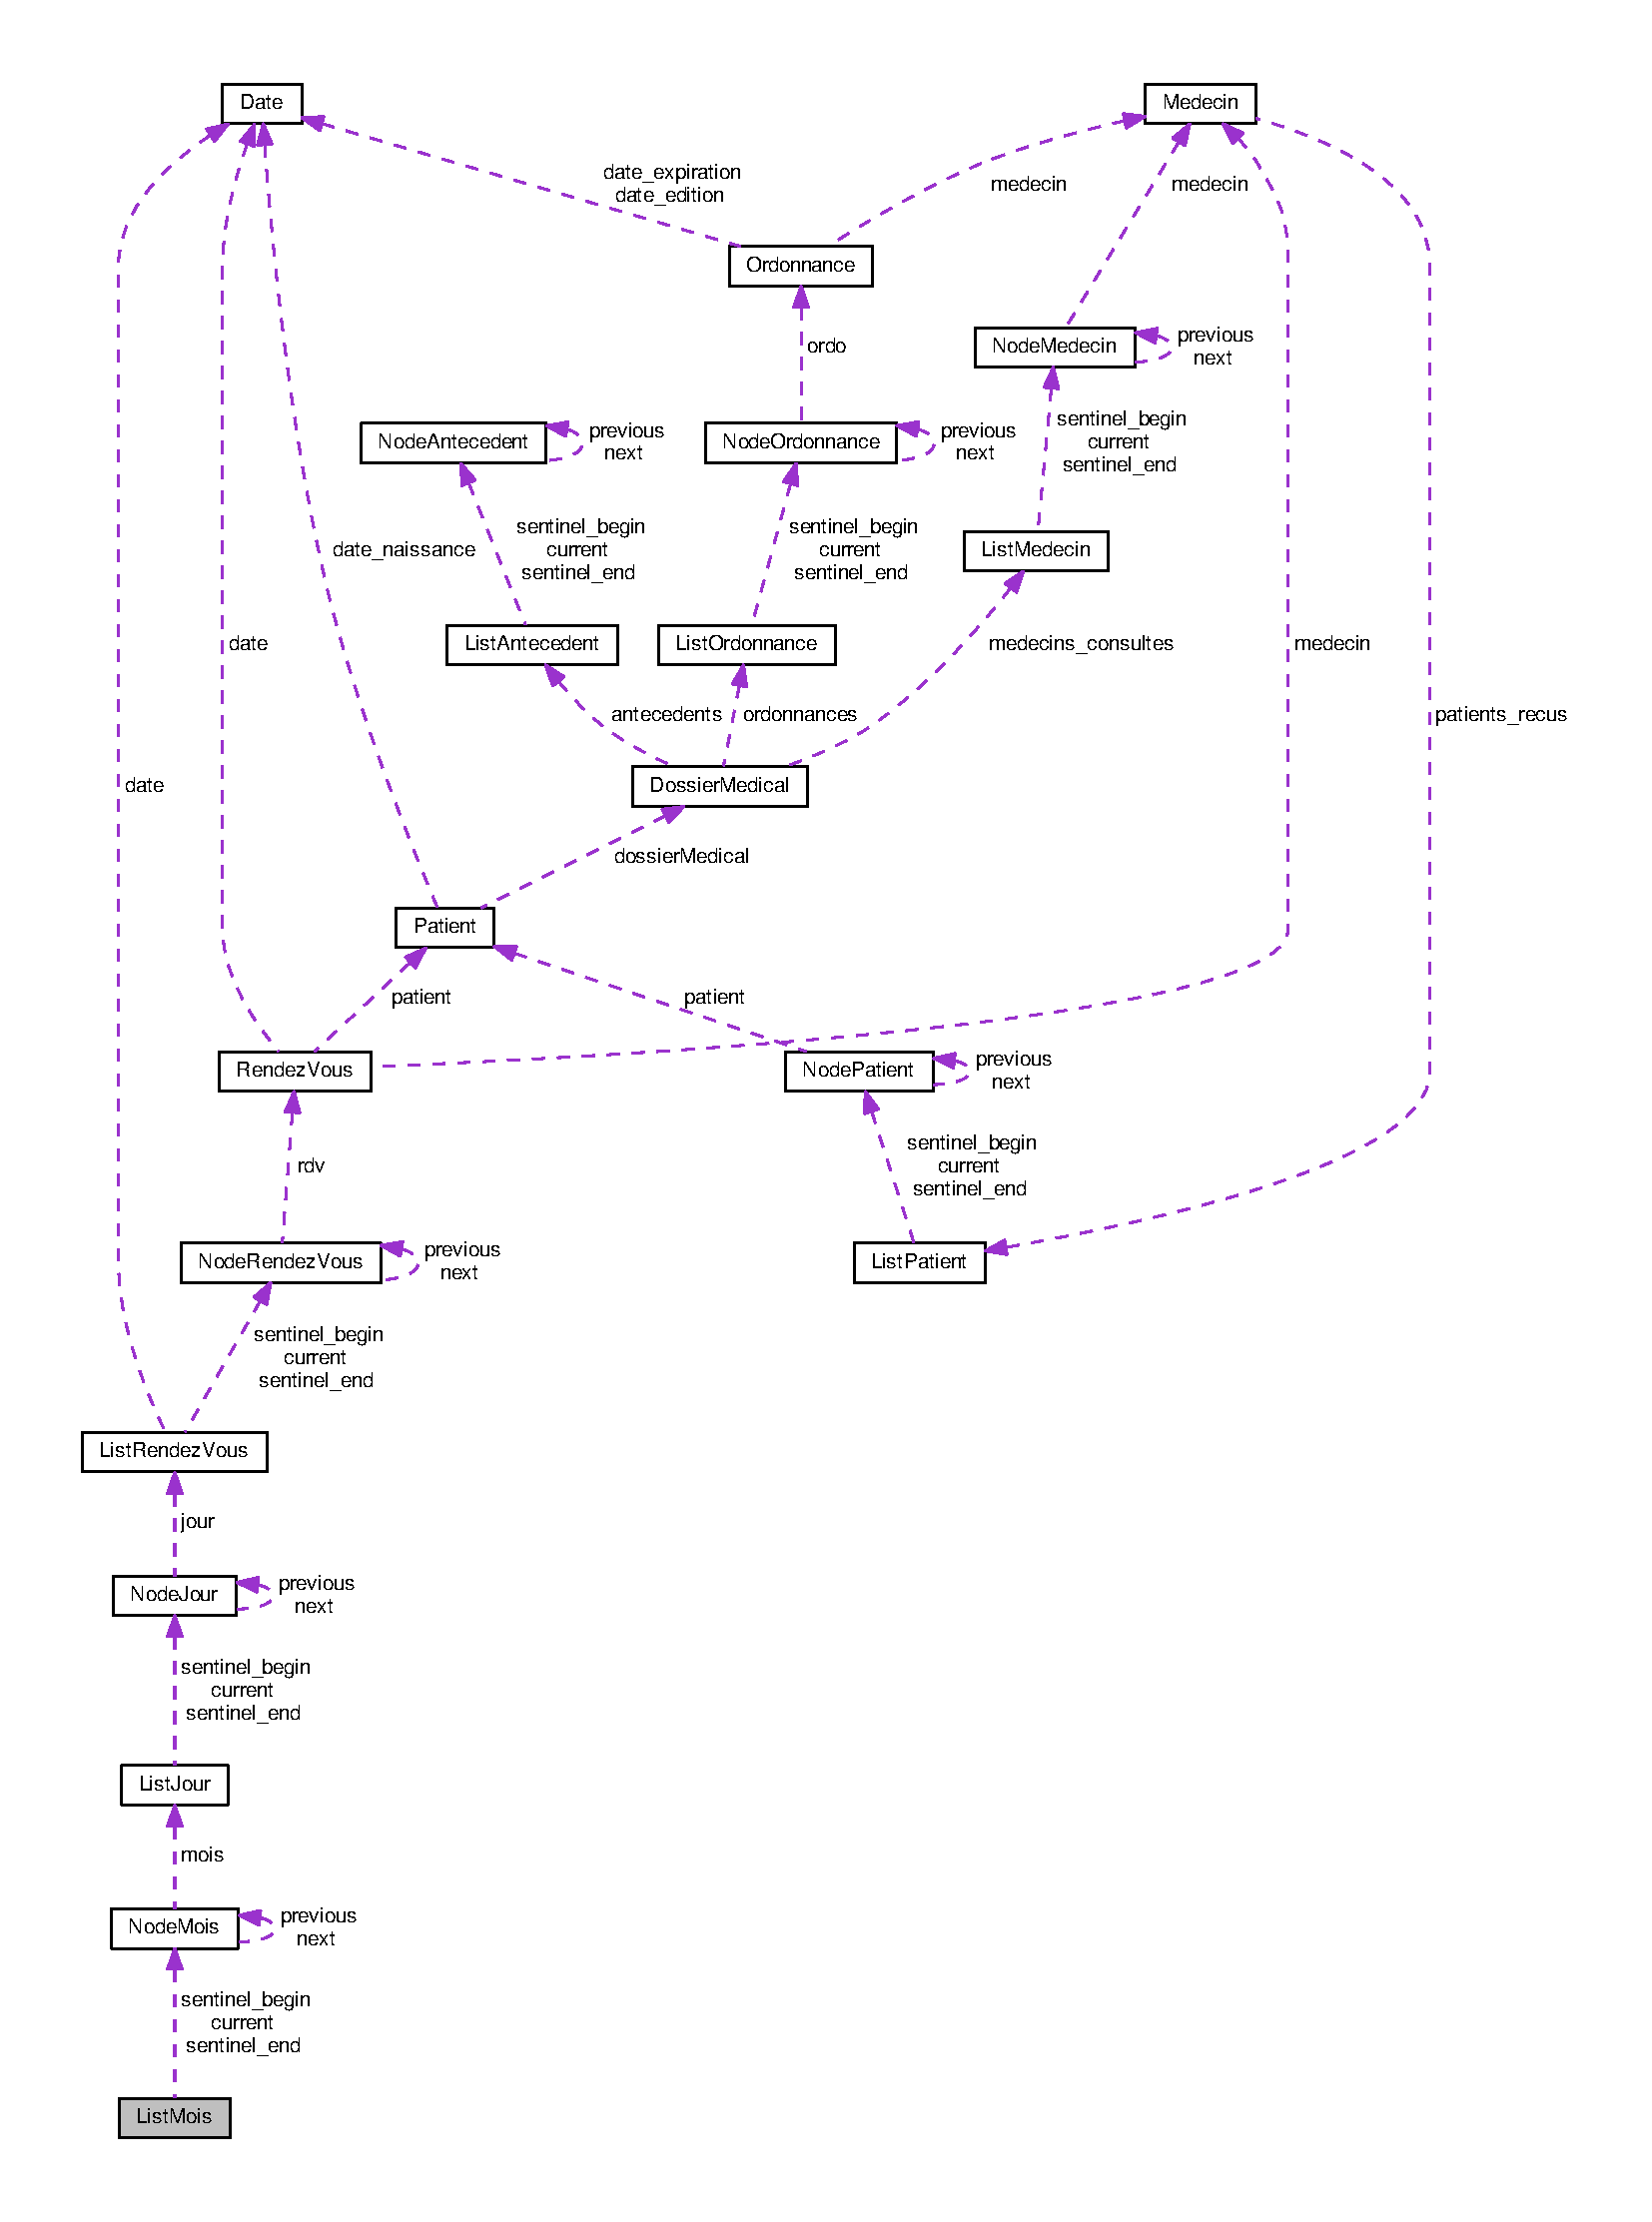
\includegraphics[width=350pt]{struct_list_mois__coll__graph}
\end{center}
\end{figure}
\subsection*{Champs de données}
\begin{DoxyCompactItemize}
\item 
int \hyperlink{struct_list_mois_acfe2ff64f5396827db36f1575c5e99d8}{annee}
\item 
\hyperlink{struct_node_mois}{Node\-Mois} \hyperlink{struct_list_mois_a348d32e033fef5b956bbd0470f22a50c}{sentinel\-\_\-begin}
\item 
\hyperlink{struct_node_mois}{Node\-Mois} $\ast$ \hyperlink{struct_list_mois_a5b776be43208a3cfeec9d21bf0fe0624}{current}
\item 
\hyperlink{struct_node_mois}{Node\-Mois} \hyperlink{struct_list_mois_abcefbcec0ea15d4123448b26256468fe}{sentinel\-\_\-end}
\end{DoxyCompactItemize}


\subsection{Documentation des champs}
\hypertarget{struct_list_mois_acfe2ff64f5396827db36f1575c5e99d8}{\index{List\-Mois@{List\-Mois}!annee@{annee}}
\index{annee@{annee}!ListMois@{List\-Mois}}
\subsubsection[{annee}]{\setlength{\rightskip}{0pt plus 5cm}int annee}}\label{struct_list_mois_acfe2ff64f5396827db36f1575c5e99d8}
\hypertarget{struct_list_mois_a5b776be43208a3cfeec9d21bf0fe0624}{\index{List\-Mois@{List\-Mois}!current@{current}}
\index{current@{current}!ListMois@{List\-Mois}}
\subsubsection[{current}]{\setlength{\rightskip}{0pt plus 5cm}{\bf Node\-Mois}$\ast$ current}}\label{struct_list_mois_a5b776be43208a3cfeec9d21bf0fe0624}
\hypertarget{struct_list_mois_a348d32e033fef5b956bbd0470f22a50c}{\index{List\-Mois@{List\-Mois}!sentinel\-\_\-begin@{sentinel\-\_\-begin}}
\index{sentinel\-\_\-begin@{sentinel\-\_\-begin}!ListMois@{List\-Mois}}
\subsubsection[{sentinel\-\_\-begin}]{\setlength{\rightskip}{0pt plus 5cm}{\bf Node\-Mois} sentinel\-\_\-begin}}\label{struct_list_mois_a348d32e033fef5b956bbd0470f22a50c}
\hypertarget{struct_list_mois_abcefbcec0ea15d4123448b26256468fe}{\index{List\-Mois@{List\-Mois}!sentinel\-\_\-end@{sentinel\-\_\-end}}
\index{sentinel\-\_\-end@{sentinel\-\_\-end}!ListMois@{List\-Mois}}
\subsubsection[{sentinel\-\_\-end}]{\setlength{\rightskip}{0pt plus 5cm}{\bf Node\-Mois} sentinel\-\_\-end}}\label{struct_list_mois_abcefbcec0ea15d4123448b26256468fe}


La documentation de cette structure a été générée à partir du fichier suivant \-:\begin{DoxyCompactItemize}
\item 
include/\-G\-P\-Calendar/\-Model/\hyperlink{calendrier_8h}{calendrier.\-h}\end{DoxyCompactItemize}

\hypertarget{struct_list_ordonnance}{\section{Référence de la structure List\-Ordonnance}
\label{struct_list_ordonnance}\index{List\-Ordonnance@{List\-Ordonnance}}
}


{\ttfamily \#include $<$ordonnance.\-h$>$}



Graphe de collaboration de List\-Ordonnance\-:
\nopagebreak
\begin{figure}[H]
\begin{center}
\leavevmode
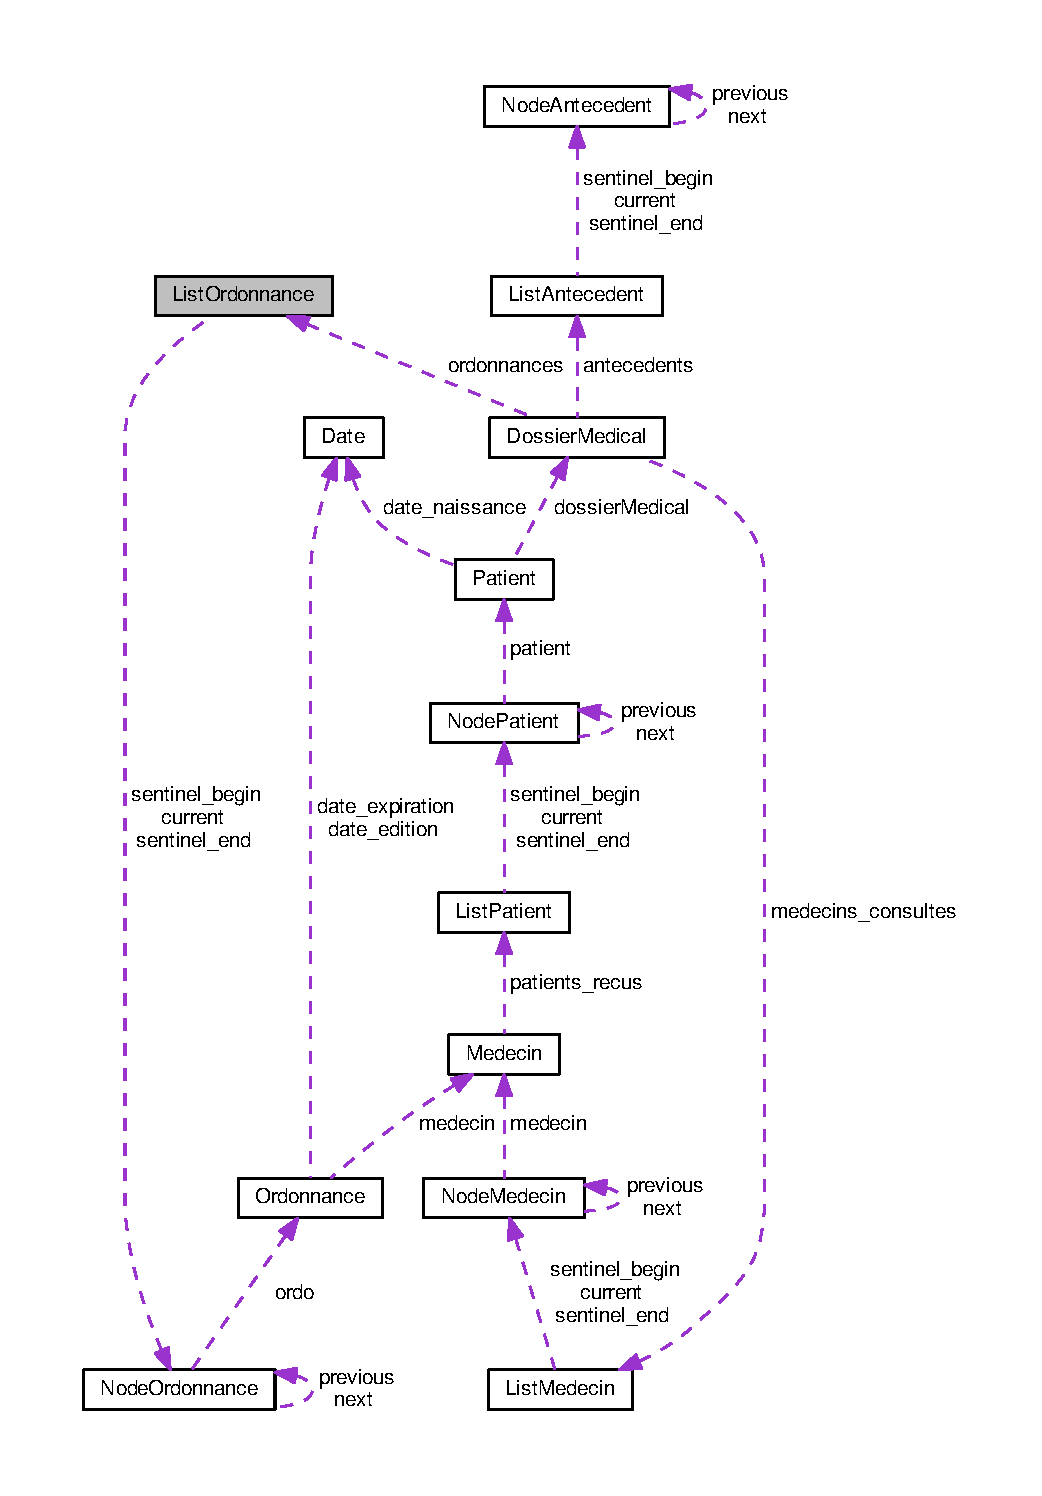
\includegraphics[width=350pt]{struct_list_ordonnance__coll__graph}
\end{center}
\end{figure}
\subsection*{Champs de données}
\begin{DoxyCompactItemize}
\item 
\hyperlink{struct_node_ordonnance}{Node\-Ordonnance} \hyperlink{struct_list_ordonnance_a364d17b110f618a202d1e1d49f0d7ca8}{sentinel\-\_\-begin}
\item 
\hyperlink{struct_node_ordonnance}{Node\-Ordonnance} $\ast$ \hyperlink{struct_list_ordonnance_a1cf97af157701a64fc159222fd9b473b}{current}
\item 
\hyperlink{struct_node_ordonnance}{Node\-Ordonnance} \hyperlink{struct_list_ordonnance_a5ca6db7384d3a5276609a826a5576204}{sentinel\-\_\-end}
\end{DoxyCompactItemize}


\subsection{Documentation des champs}
\hypertarget{struct_list_ordonnance_a1cf97af157701a64fc159222fd9b473b}{\index{List\-Ordonnance@{List\-Ordonnance}!current@{current}}
\index{current@{current}!ListOrdonnance@{List\-Ordonnance}}
\subsubsection[{current}]{\setlength{\rightskip}{0pt plus 5cm}{\bf Node\-Ordonnance}$\ast$ current}}\label{struct_list_ordonnance_a1cf97af157701a64fc159222fd9b473b}
\hypertarget{struct_list_ordonnance_a364d17b110f618a202d1e1d49f0d7ca8}{\index{List\-Ordonnance@{List\-Ordonnance}!sentinel\-\_\-begin@{sentinel\-\_\-begin}}
\index{sentinel\-\_\-begin@{sentinel\-\_\-begin}!ListOrdonnance@{List\-Ordonnance}}
\subsubsection[{sentinel\-\_\-begin}]{\setlength{\rightskip}{0pt plus 5cm}{\bf Node\-Ordonnance} sentinel\-\_\-begin}}\label{struct_list_ordonnance_a364d17b110f618a202d1e1d49f0d7ca8}
\hypertarget{struct_list_ordonnance_a5ca6db7384d3a5276609a826a5576204}{\index{List\-Ordonnance@{List\-Ordonnance}!sentinel\-\_\-end@{sentinel\-\_\-end}}
\index{sentinel\-\_\-end@{sentinel\-\_\-end}!ListOrdonnance@{List\-Ordonnance}}
\subsubsection[{sentinel\-\_\-end}]{\setlength{\rightskip}{0pt plus 5cm}{\bf Node\-Ordonnance} sentinel\-\_\-end}}\label{struct_list_ordonnance_a5ca6db7384d3a5276609a826a5576204}


La documentation de cette structure a été générée à partir du fichier suivant \-:\begin{DoxyCompactItemize}
\item 
include/\-G\-P\-Calendar/\-Model/\hyperlink{ordonnance_8h}{ordonnance.\-h}\end{DoxyCompactItemize}

\hypertarget{struct_list_patient}{\section{Référence de la structure List\-Patient}
\label{struct_list_patient}\index{List\-Patient@{List\-Patient}}
}


{\ttfamily \#include $<$patient.\-h$>$}



Graphe de collaboration de List\-Patient\-:
\nopagebreak
\begin{figure}[H]
\begin{center}
\leavevmode
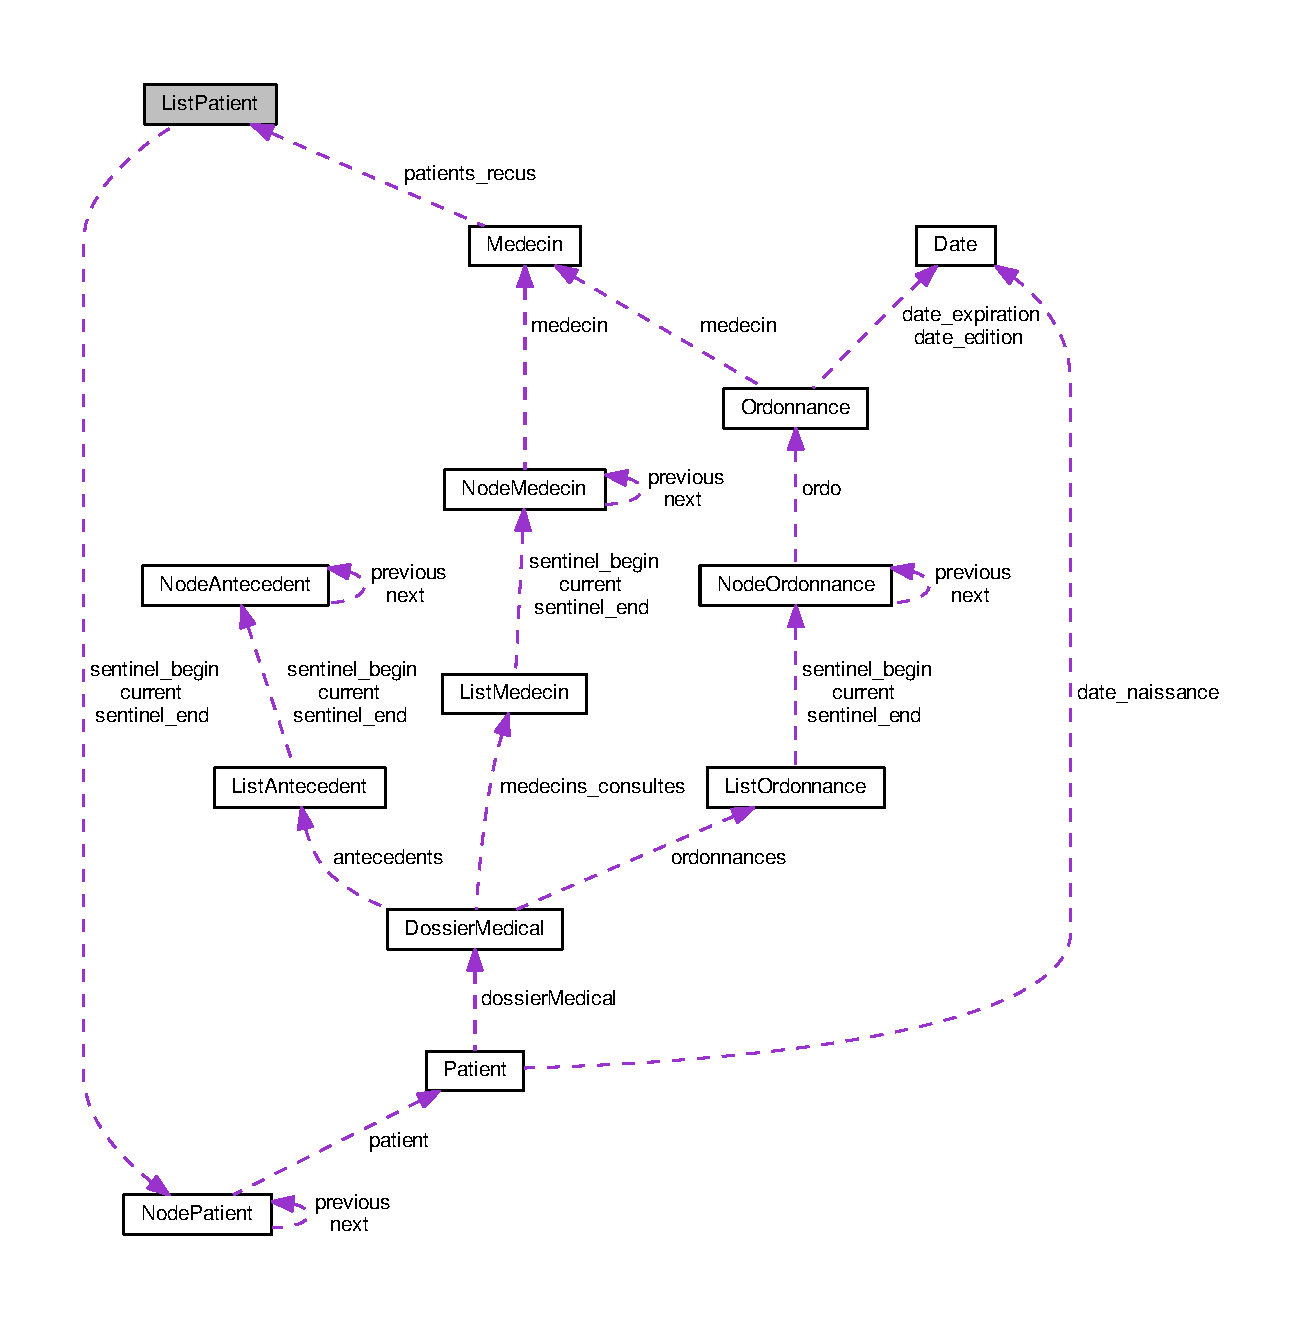
\includegraphics[width=350pt]{struct_list_patient__coll__graph}
\end{center}
\end{figure}
\subsection*{Champs de données}
\begin{DoxyCompactItemize}
\item 
\hyperlink{struct_node_patient}{Node\-Patient} \hyperlink{struct_list_patient_acacbc6137b28bb2b48b0a2cfe4305024}{sentinel\-\_\-begin}
\item 
\hyperlink{struct_node_patient}{Node\-Patient} $\ast$ \hyperlink{struct_list_patient_ae1c66e6952e3fd81efd6fe0f72a51826}{current}
\item 
\hyperlink{struct_node_patient}{Node\-Patient} \hyperlink{struct_list_patient_ad2cb1194a61ed31c401c99218ff6dbb7}{sentinel\-\_\-end}
\end{DoxyCompactItemize}


\subsection{Documentation des champs}
\hypertarget{struct_list_patient_ae1c66e6952e3fd81efd6fe0f72a51826}{\index{List\-Patient@{List\-Patient}!current@{current}}
\index{current@{current}!ListPatient@{List\-Patient}}
\subsubsection[{current}]{\setlength{\rightskip}{0pt plus 5cm}{\bf Node\-Patient}$\ast$ current}}\label{struct_list_patient_ae1c66e6952e3fd81efd6fe0f72a51826}
\hypertarget{struct_list_patient_acacbc6137b28bb2b48b0a2cfe4305024}{\index{List\-Patient@{List\-Patient}!sentinel\-\_\-begin@{sentinel\-\_\-begin}}
\index{sentinel\-\_\-begin@{sentinel\-\_\-begin}!ListPatient@{List\-Patient}}
\subsubsection[{sentinel\-\_\-begin}]{\setlength{\rightskip}{0pt plus 5cm}{\bf Node\-Patient} sentinel\-\_\-begin}}\label{struct_list_patient_acacbc6137b28bb2b48b0a2cfe4305024}
\hypertarget{struct_list_patient_ad2cb1194a61ed31c401c99218ff6dbb7}{\index{List\-Patient@{List\-Patient}!sentinel\-\_\-end@{sentinel\-\_\-end}}
\index{sentinel\-\_\-end@{sentinel\-\_\-end}!ListPatient@{List\-Patient}}
\subsubsection[{sentinel\-\_\-end}]{\setlength{\rightskip}{0pt plus 5cm}{\bf Node\-Patient} sentinel\-\_\-end}}\label{struct_list_patient_ad2cb1194a61ed31c401c99218ff6dbb7}


La documentation de cette structure a été générée à partir du fichier suivant \-:\begin{DoxyCompactItemize}
\item 
include/\-G\-P\-Calendar/\-Model/\hyperlink{patient_8h}{patient.\-h}\end{DoxyCompactItemize}

\hypertarget{struct_list_rendez_vous}{\section{Référence de la structure List\-Rendez\-Vous}
\label{struct_list_rendez_vous}\index{List\-Rendez\-Vous@{List\-Rendez\-Vous}}
}


{\ttfamily \#include $<$calendrier.\-h$>$}



Graphe de collaboration de List\-Rendez\-Vous\-:
\nopagebreak
\begin{figure}[H]
\begin{center}
\leavevmode
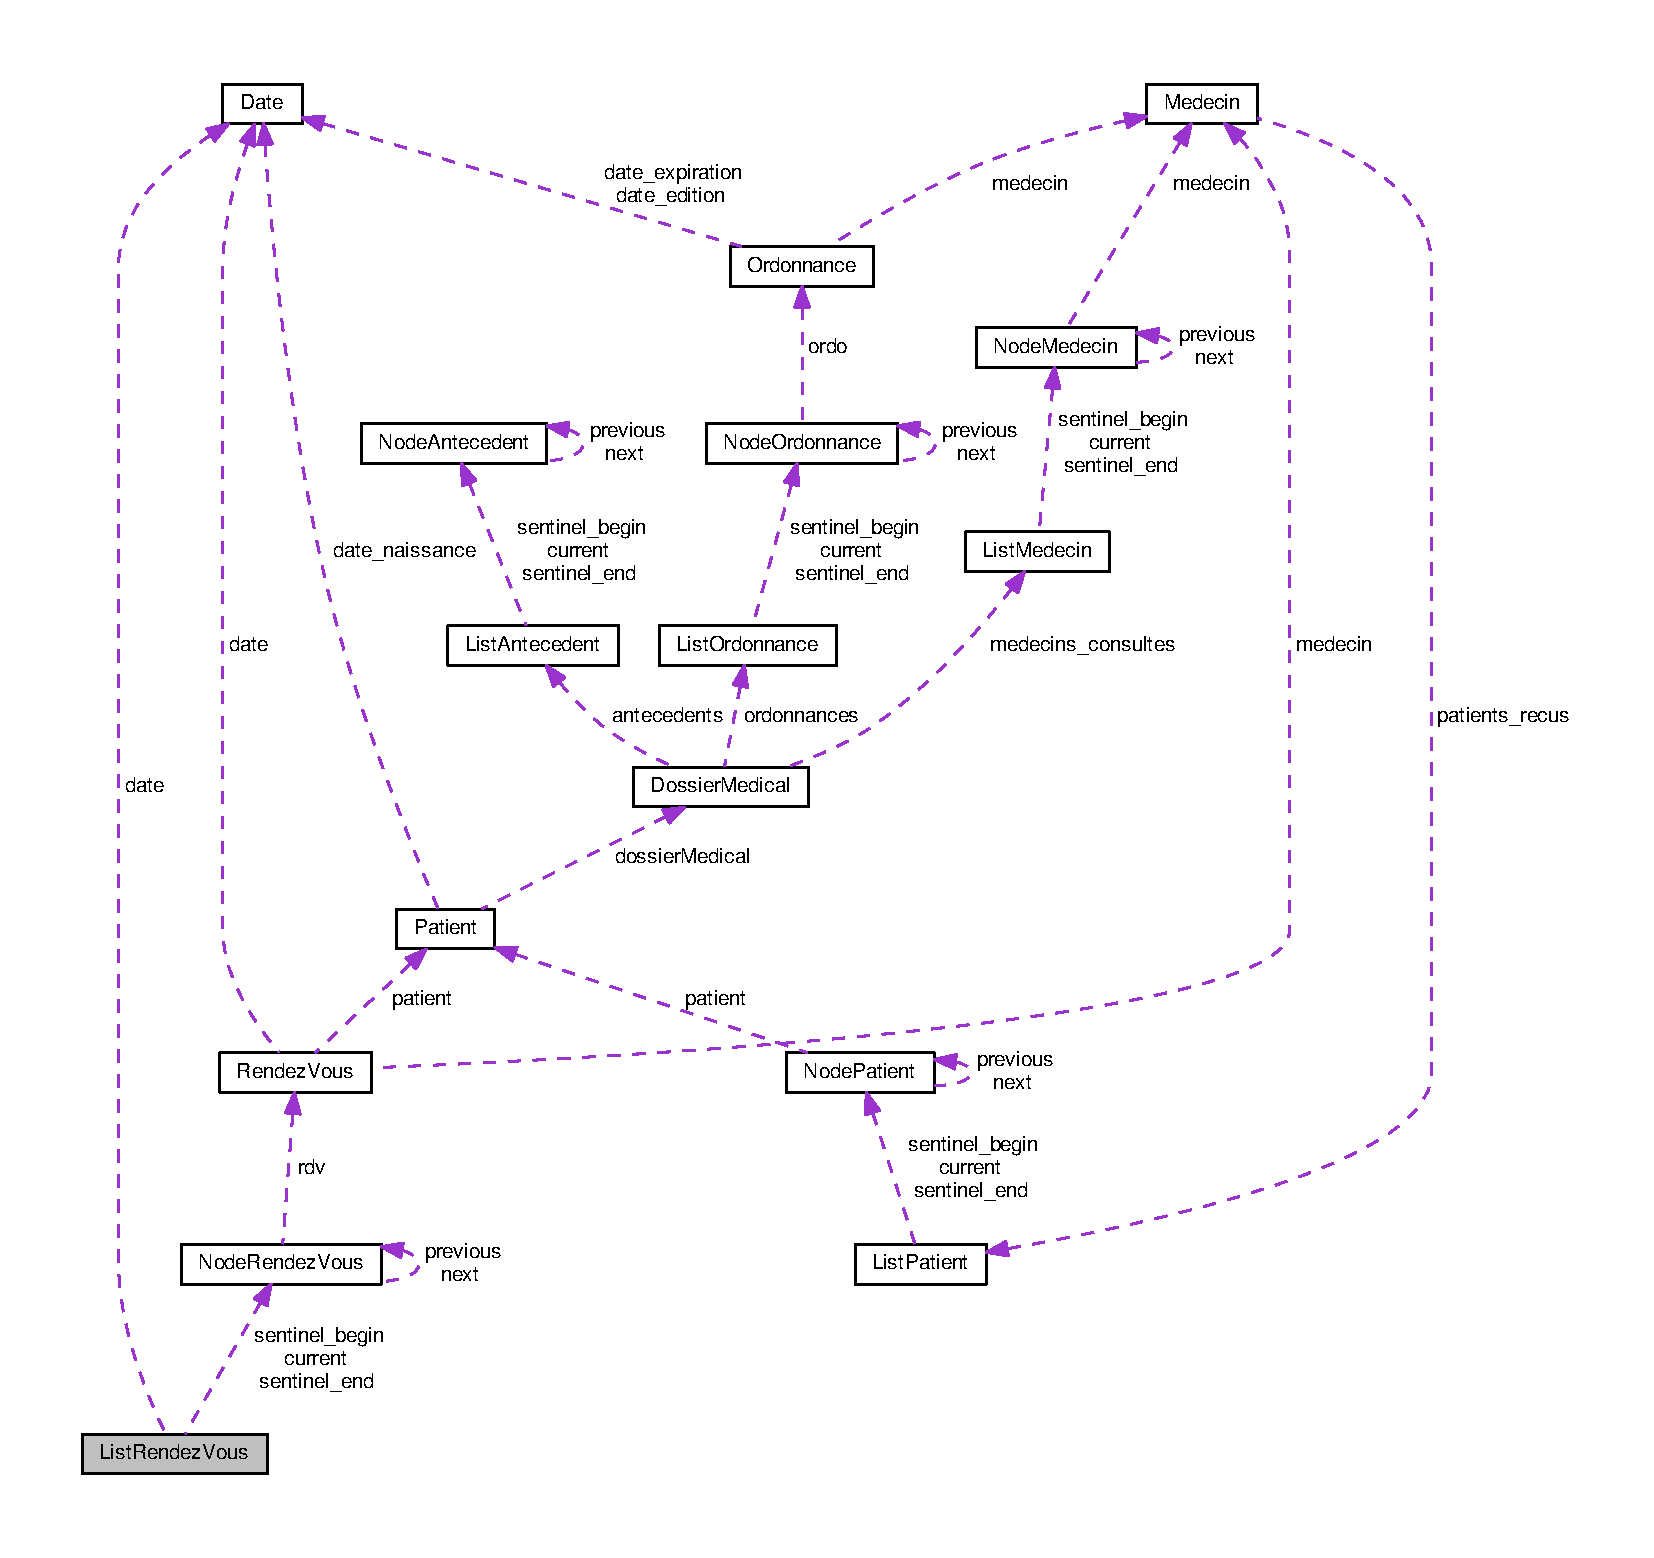
\includegraphics[width=350pt]{struct_list_rendez_vous__coll__graph}
\end{center}
\end{figure}
\subsection*{Champs de données}
\begin{DoxyCompactItemize}
\item 
\hyperlink{struct_date}{Date} $\ast$ \hyperlink{struct_list_rendez_vous_a73fc78564c9badbcea68f2f2331c74db}{date}
\item 
\hyperlink{struct_node_rendez_vous}{Node\-Rendez\-Vous} \hyperlink{struct_list_rendez_vous_a557d4ad3f27cc277dbd188dd7edc897c}{sentinel\-\_\-begin}
\item 
\hyperlink{struct_node_rendez_vous}{Node\-Rendez\-Vous} $\ast$ \hyperlink{struct_list_rendez_vous_af4abed97401227a9dc25377d0840dd36}{current}
\item 
\hyperlink{struct_node_rendez_vous}{Node\-Rendez\-Vous} \hyperlink{struct_list_rendez_vous_a23ecc58b8762108d2cdf8d71b1848178}{sentinel\-\_\-end}
\end{DoxyCompactItemize}


\subsection{Documentation des champs}
\hypertarget{struct_list_rendez_vous_af4abed97401227a9dc25377d0840dd36}{\index{List\-Rendez\-Vous@{List\-Rendez\-Vous}!current@{current}}
\index{current@{current}!ListRendezVous@{List\-Rendez\-Vous}}
\subsubsection[{current}]{\setlength{\rightskip}{0pt plus 5cm}{\bf Node\-Rendez\-Vous}$\ast$ current}}\label{struct_list_rendez_vous_af4abed97401227a9dc25377d0840dd36}
\hypertarget{struct_list_rendez_vous_a73fc78564c9badbcea68f2f2331c74db}{\index{List\-Rendez\-Vous@{List\-Rendez\-Vous}!date@{date}}
\index{date@{date}!ListRendezVous@{List\-Rendez\-Vous}}
\subsubsection[{date}]{\setlength{\rightskip}{0pt plus 5cm}{\bf Date}$\ast$ date}}\label{struct_list_rendez_vous_a73fc78564c9badbcea68f2f2331c74db}
\hypertarget{struct_list_rendez_vous_a557d4ad3f27cc277dbd188dd7edc897c}{\index{List\-Rendez\-Vous@{List\-Rendez\-Vous}!sentinel\-\_\-begin@{sentinel\-\_\-begin}}
\index{sentinel\-\_\-begin@{sentinel\-\_\-begin}!ListRendezVous@{List\-Rendez\-Vous}}
\subsubsection[{sentinel\-\_\-begin}]{\setlength{\rightskip}{0pt plus 5cm}{\bf Node\-Rendez\-Vous} sentinel\-\_\-begin}}\label{struct_list_rendez_vous_a557d4ad3f27cc277dbd188dd7edc897c}
\hypertarget{struct_list_rendez_vous_a23ecc58b8762108d2cdf8d71b1848178}{\index{List\-Rendez\-Vous@{List\-Rendez\-Vous}!sentinel\-\_\-end@{sentinel\-\_\-end}}
\index{sentinel\-\_\-end@{sentinel\-\_\-end}!ListRendezVous@{List\-Rendez\-Vous}}
\subsubsection[{sentinel\-\_\-end}]{\setlength{\rightskip}{0pt plus 5cm}{\bf Node\-Rendez\-Vous} sentinel\-\_\-end}}\label{struct_list_rendez_vous_a23ecc58b8762108d2cdf8d71b1848178}


La documentation de cette structure a été générée à partir du fichier suivant \-:\begin{DoxyCompactItemize}
\item 
include/\-G\-P\-Calendar/\-Model/\hyperlink{calendrier_8h}{calendrier.\-h}\end{DoxyCompactItemize}

\hypertarget{struct_medecin}{\section{Référence de la structure Medecin}
\label{struct_medecin}\index{Medecin@{Medecin}}
}


{\ttfamily \#include $<$medecin.\-h$>$}



Graphe de collaboration de Medecin\-:
\nopagebreak
\begin{figure}[H]
\begin{center}
\leavevmode
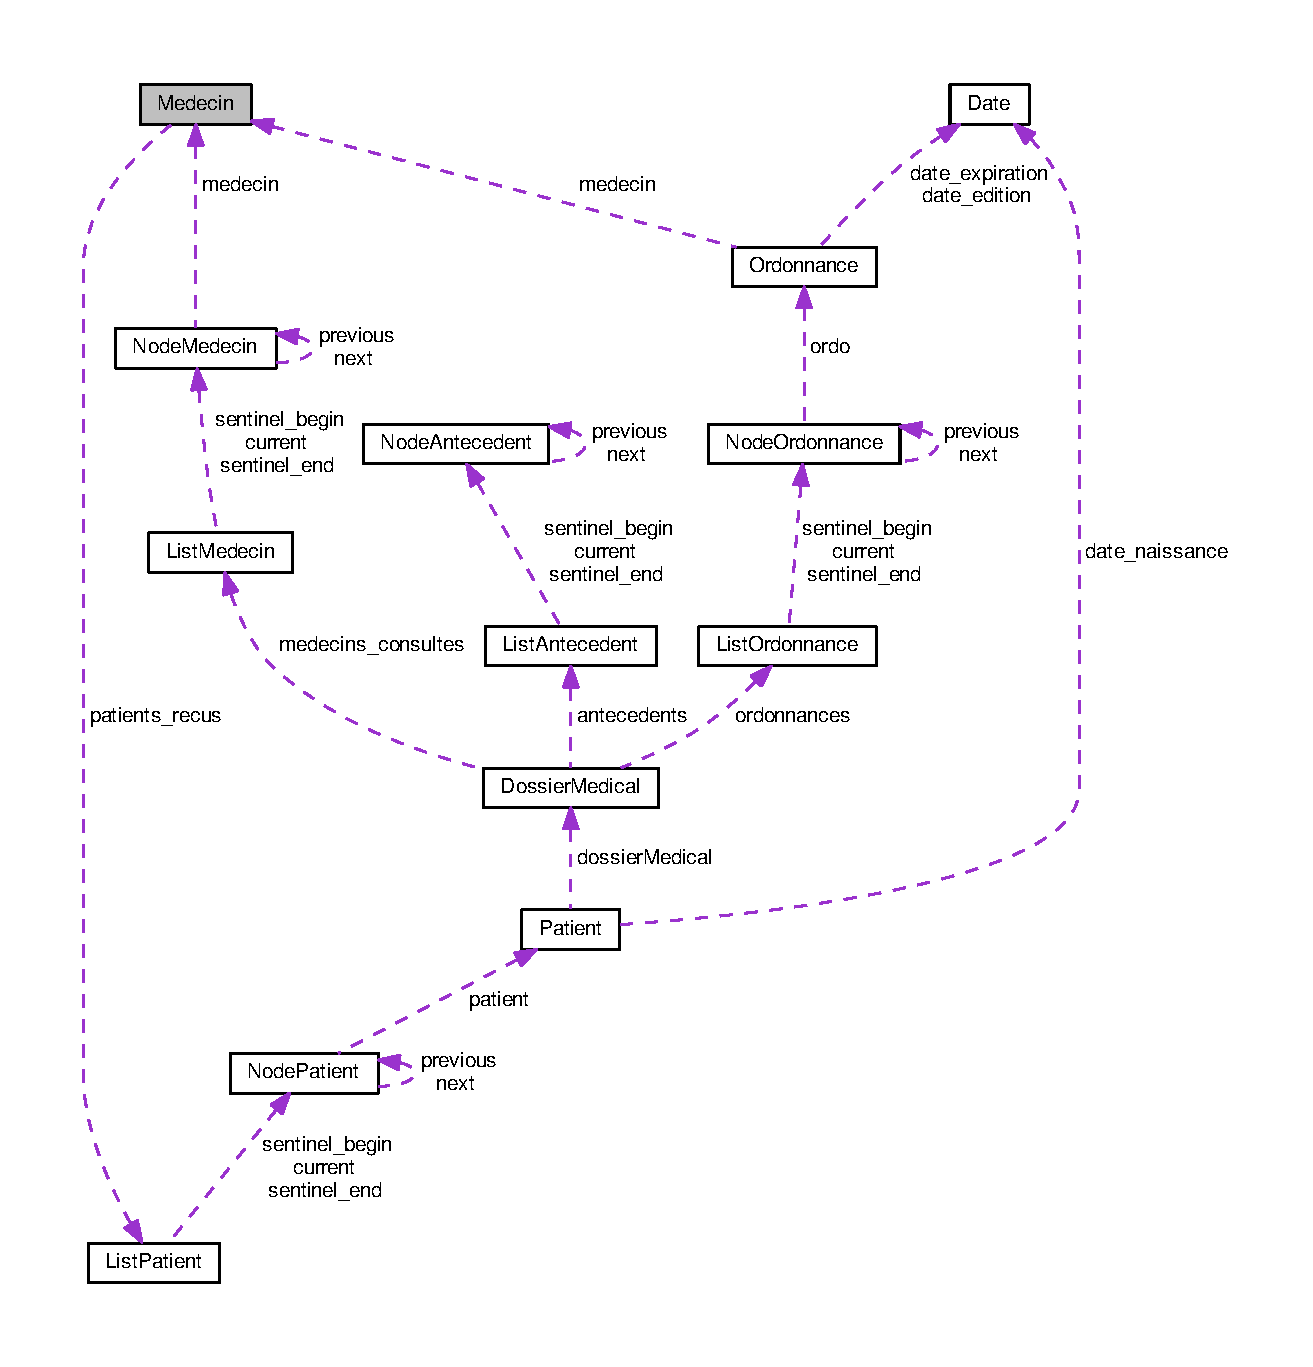
\includegraphics[width=350pt]{struct_medecin__coll__graph}
\end{center}
\end{figure}
\subsection*{Champs de données}
\begin{DoxyCompactItemize}
\item 
char $\ast$ \hyperlink{struct_medecin_abe308d273ff51ad86ff02ef3ba3b6f0e}{nom}
\item 
char $\ast$ \hyperlink{struct_medecin_aa7d0e9e8505d2ac627777c4168573ec9}{prenom}
\item 
char $\ast$$\ast$ \hyperlink{struct_medecin_a65fe6337893c03f2e41cba9f4fe45dd0}{specialites}
\item 
char $\ast$$\ast$ \hyperlink{struct_medecin_a30acb0c2b918d1f2a3bac4b758474832}{diplomes}
\item 
char $\ast$ \hyperlink{struct_medecin_aefa944e4b78fb9e14c4f6e49605bba2c}{adresse\-\_\-mail}
\item 
char $\ast$ \hyperlink{struct_medecin_ac65f93b2b15c34c800c05832e346c98f}{numero\-\_\-telephone}
\item 
char $\ast$ \hyperlink{struct_medecin_aef3cdf238a67d175fecba3f7df4e6828}{numero\-\_\-\-R\-P\-S}
\item 
struct \hyperlink{struct_list_patient}{List\-Patient} $\ast$ \hyperlink{struct_medecin_ad1dc0fd5fced379618573f857d441736}{patients\-\_\-recus}
\end{DoxyCompactItemize}


\subsection{Description détaillée}
Structure \hyperlink{struct_medecin}{Medecin} représentant un \hyperlink{struct_medecin}{Medecin} exercant dans l'hopital 

\subsection{Documentation des champs}
\hypertarget{struct_medecin_aefa944e4b78fb9e14c4f6e49605bba2c}{\index{Medecin@{Medecin}!adresse\-\_\-mail@{adresse\-\_\-mail}}
\index{adresse\-\_\-mail@{adresse\-\_\-mail}!Medecin@{Medecin}}
\subsubsection[{adresse\-\_\-mail}]{\setlength{\rightskip}{0pt plus 5cm}char$\ast$ adresse\-\_\-mail}}\label{struct_medecin_aefa944e4b78fb9e14c4f6e49605bba2c}
\hypertarget{struct_medecin_a30acb0c2b918d1f2a3bac4b758474832}{\index{Medecin@{Medecin}!diplomes@{diplomes}}
\index{diplomes@{diplomes}!Medecin@{Medecin}}
\subsubsection[{diplomes}]{\setlength{\rightskip}{0pt plus 5cm}char$\ast$$\ast$ diplomes}}\label{struct_medecin_a30acb0c2b918d1f2a3bac4b758474832}
\hypertarget{struct_medecin_abe308d273ff51ad86ff02ef3ba3b6f0e}{\index{Medecin@{Medecin}!nom@{nom}}
\index{nom@{nom}!Medecin@{Medecin}}
\subsubsection[{nom}]{\setlength{\rightskip}{0pt plus 5cm}char$\ast$ nom}}\label{struct_medecin_abe308d273ff51ad86ff02ef3ba3b6f0e}
\hypertarget{struct_medecin_aef3cdf238a67d175fecba3f7df4e6828}{\index{Medecin@{Medecin}!numero\-\_\-\-R\-P\-S@{numero\-\_\-\-R\-P\-S}}
\index{numero\-\_\-\-R\-P\-S@{numero\-\_\-\-R\-P\-S}!Medecin@{Medecin}}
\subsubsection[{numero\-\_\-\-R\-P\-S}]{\setlength{\rightskip}{0pt plus 5cm}char$\ast$ numero\-\_\-\-R\-P\-S}}\label{struct_medecin_aef3cdf238a67d175fecba3f7df4e6828}
\hypertarget{struct_medecin_ac65f93b2b15c34c800c05832e346c98f}{\index{Medecin@{Medecin}!numero\-\_\-telephone@{numero\-\_\-telephone}}
\index{numero\-\_\-telephone@{numero\-\_\-telephone}!Medecin@{Medecin}}
\subsubsection[{numero\-\_\-telephone}]{\setlength{\rightskip}{0pt plus 5cm}char$\ast$ numero\-\_\-telephone}}\label{struct_medecin_ac65f93b2b15c34c800c05832e346c98f}
\hypertarget{struct_medecin_ad1dc0fd5fced379618573f857d441736}{\index{Medecin@{Medecin}!patients\-\_\-recus@{patients\-\_\-recus}}
\index{patients\-\_\-recus@{patients\-\_\-recus}!Medecin@{Medecin}}
\subsubsection[{patients\-\_\-recus}]{\setlength{\rightskip}{0pt plus 5cm}struct {\bf List\-Patient}$\ast$ patients\-\_\-recus}}\label{struct_medecin_ad1dc0fd5fced379618573f857d441736}
\hypertarget{struct_medecin_aa7d0e9e8505d2ac627777c4168573ec9}{\index{Medecin@{Medecin}!prenom@{prenom}}
\index{prenom@{prenom}!Medecin@{Medecin}}
\subsubsection[{prenom}]{\setlength{\rightskip}{0pt plus 5cm}char$\ast$ prenom}}\label{struct_medecin_aa7d0e9e8505d2ac627777c4168573ec9}
\hypertarget{struct_medecin_a65fe6337893c03f2e41cba9f4fe45dd0}{\index{Medecin@{Medecin}!specialites@{specialites}}
\index{specialites@{specialites}!Medecin@{Medecin}}
\subsubsection[{specialites}]{\setlength{\rightskip}{0pt plus 5cm}char$\ast$$\ast$ specialites}}\label{struct_medecin_a65fe6337893c03f2e41cba9f4fe45dd0}


La documentation de cette structure a été générée à partir du fichier suivant \-:\begin{DoxyCompactItemize}
\item 
include/\-G\-P\-Calendar/\-Model/\hyperlink{medecin_8h}{medecin.\-h}\end{DoxyCompactItemize}

\hypertarget{struct_node_annee}{\section{Référence de la structure Node\-Annee}
\label{struct_node_annee}\index{Node\-Annee@{Node\-Annee}}
}


{\ttfamily \#include $<$calendrier.\-h$>$}



Graphe de collaboration de Node\-Annee\-:
\nopagebreak
\begin{figure}[H]
\begin{center}
\leavevmode
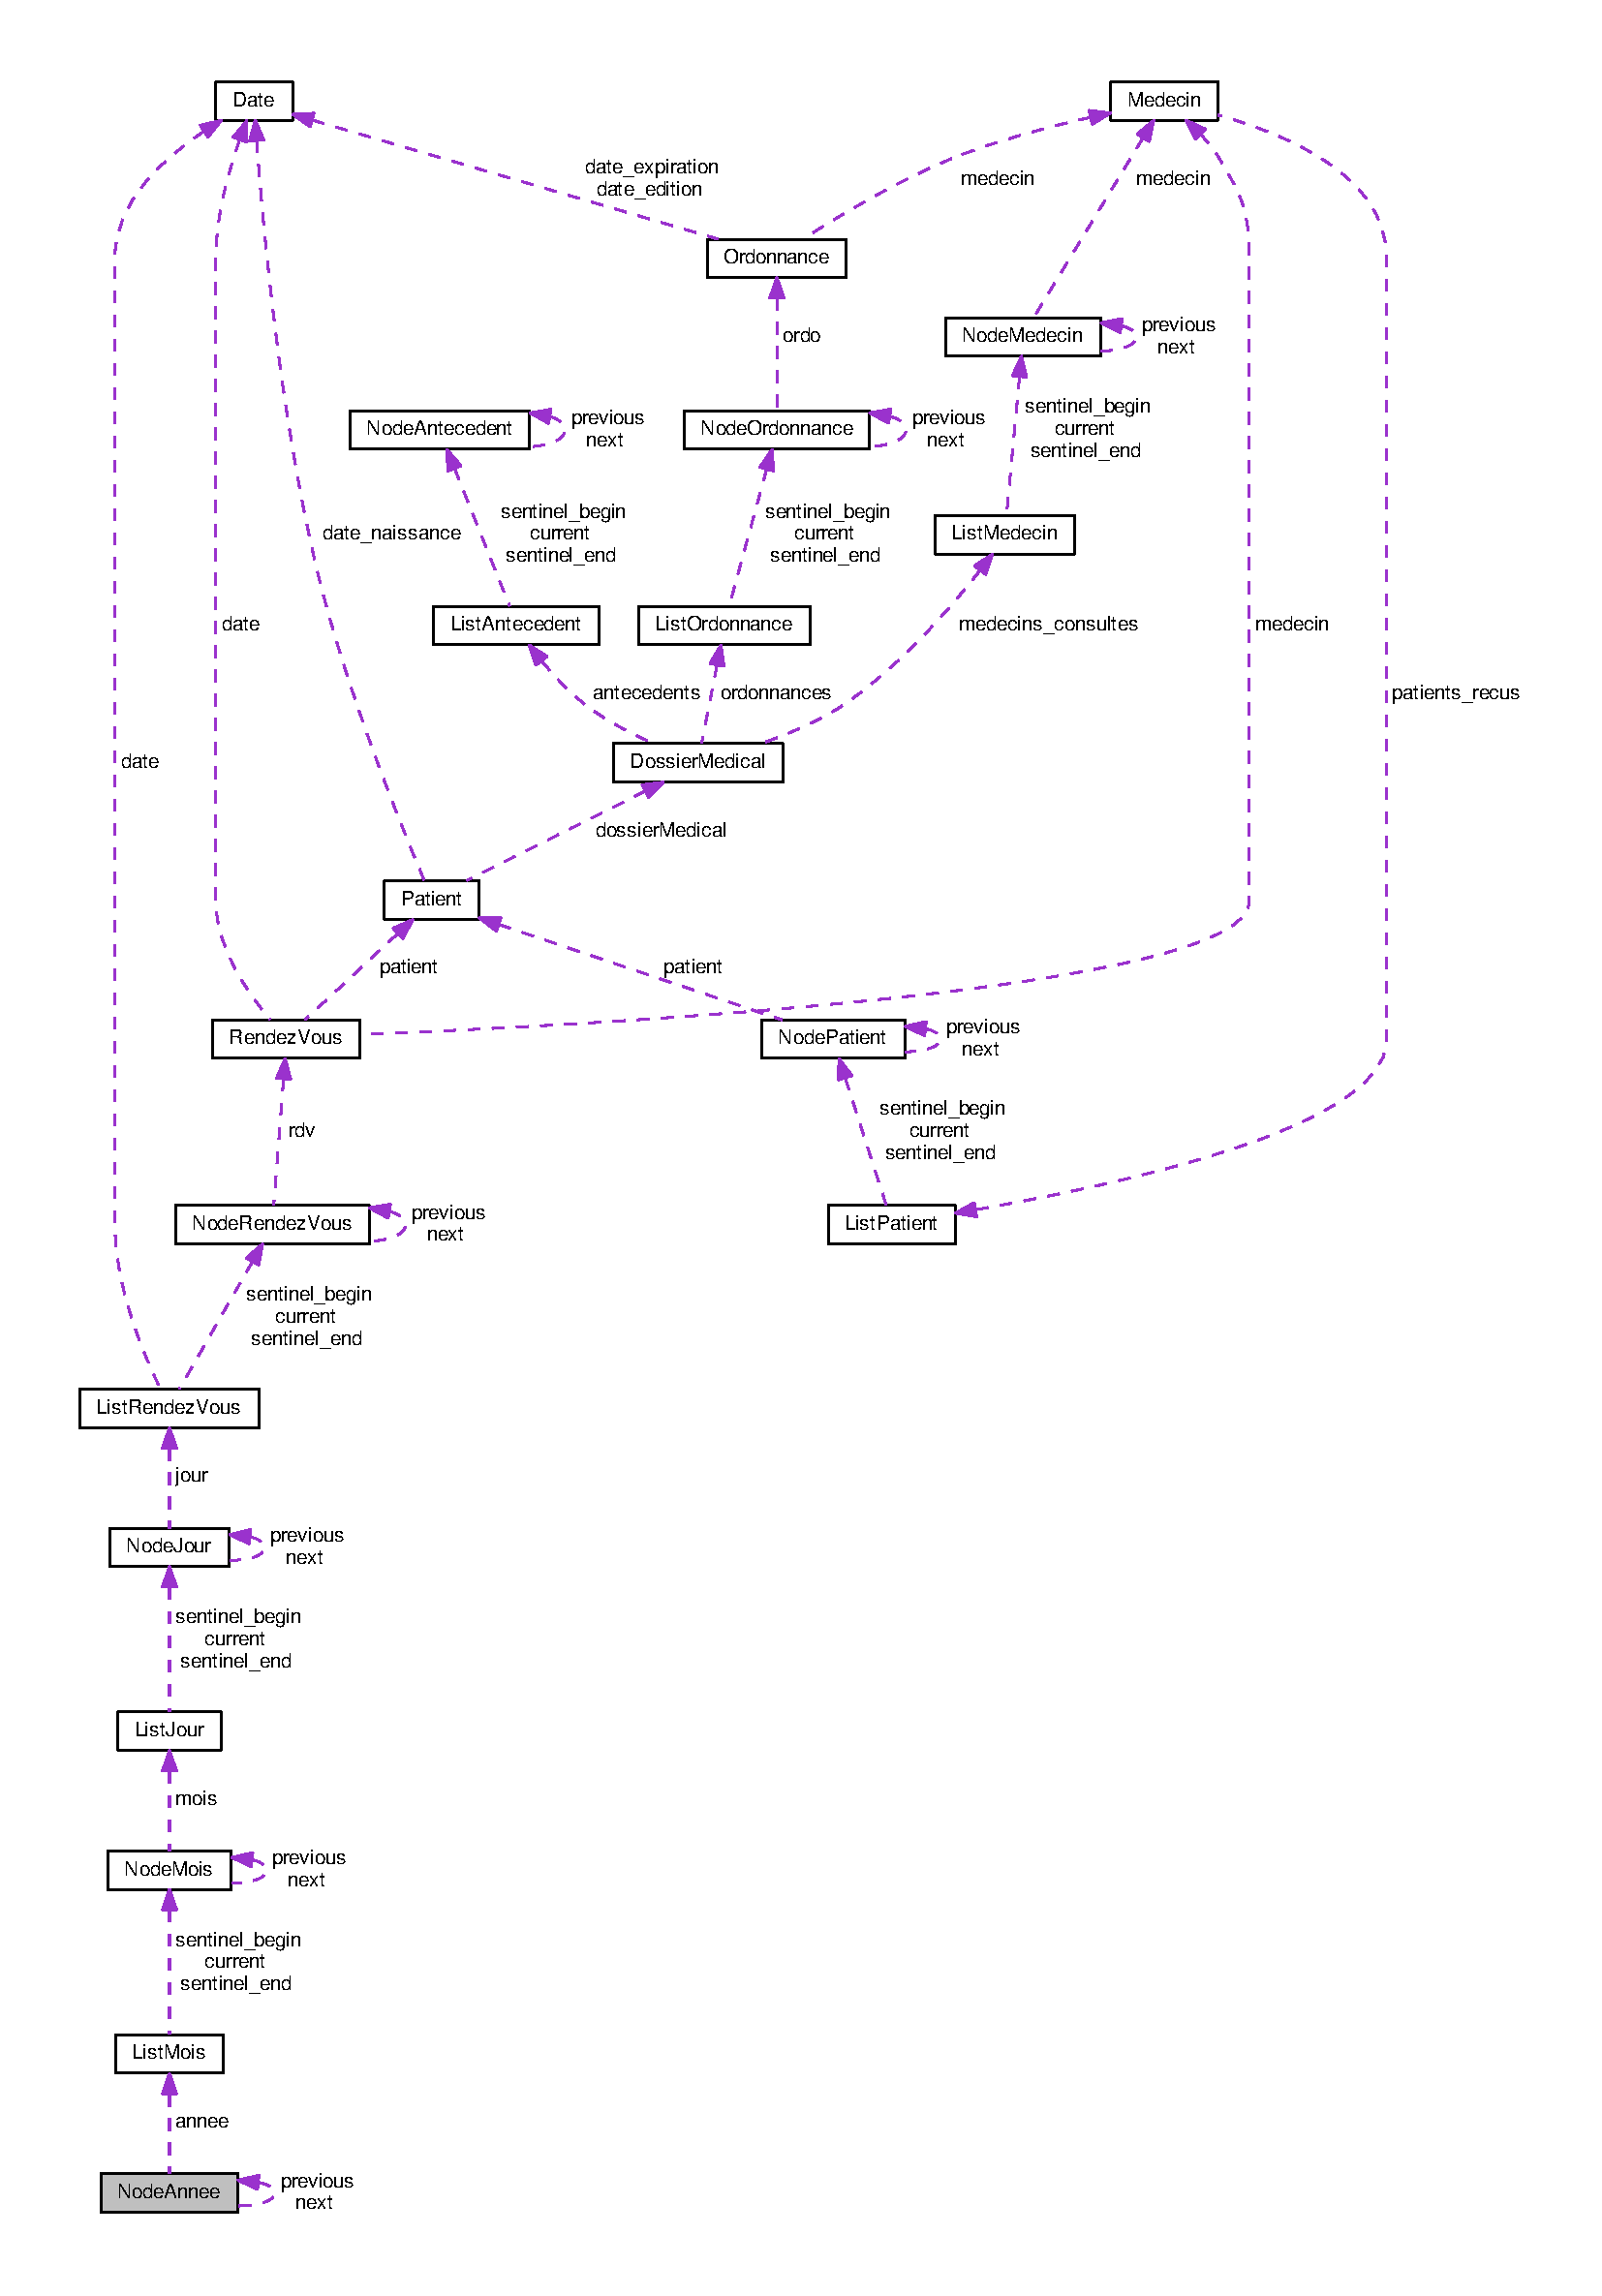
\includegraphics[width=350pt]{struct_node_annee__coll__graph}
\end{center}
\end{figure}
\subsection*{Champs de données}
\begin{DoxyCompactItemize}
\item 
\hyperlink{calendrier_8h_a8e119d682702ebf078b3235b4c0fe464}{Annee} \hyperlink{struct_node_annee_aa0898ccf3eb95fa2dc84150d887b55c1}{annee}
\item 
struct \hyperlink{struct_node_annee}{Node\-Annee} $\ast$ \hyperlink{struct_node_annee_a1cb22d42269d482585fba555db38334e}{next}
\item 
struct \hyperlink{struct_node_annee}{Node\-Annee} $\ast$ \hyperlink{struct_node_annee_aebffe5024c759df4300746c6b1034ed3}{previous}
\end{DoxyCompactItemize}


\subsection{Documentation des champs}
\hypertarget{struct_node_annee_aa0898ccf3eb95fa2dc84150d887b55c1}{\index{Node\-Annee@{Node\-Annee}!annee@{annee}}
\index{annee@{annee}!NodeAnnee@{Node\-Annee}}
\subsubsection[{annee}]{\setlength{\rightskip}{0pt plus 5cm}{\bf Annee} annee}}\label{struct_node_annee_aa0898ccf3eb95fa2dc84150d887b55c1}
\hypertarget{struct_node_annee_a1cb22d42269d482585fba555db38334e}{\index{Node\-Annee@{Node\-Annee}!next@{next}}
\index{next@{next}!NodeAnnee@{Node\-Annee}}
\subsubsection[{next}]{\setlength{\rightskip}{0pt plus 5cm}struct {\bf Node\-Annee}$\ast$ next}}\label{struct_node_annee_a1cb22d42269d482585fba555db38334e}
\hypertarget{struct_node_annee_aebffe5024c759df4300746c6b1034ed3}{\index{Node\-Annee@{Node\-Annee}!previous@{previous}}
\index{previous@{previous}!NodeAnnee@{Node\-Annee}}
\subsubsection[{previous}]{\setlength{\rightskip}{0pt plus 5cm}struct {\bf Node\-Annee}$\ast$ previous}}\label{struct_node_annee_aebffe5024c759df4300746c6b1034ed3}


La documentation de cette structure a été générée à partir du fichier suivant \-:\begin{DoxyCompactItemize}
\item 
include/\-G\-P\-Calendar/\-Model/\hyperlink{calendrier_8h}{calendrier.\-h}\end{DoxyCompactItemize}

\hypertarget{struct_node_antecedent}{\section{Référence de la structure Node\-Antecedent}
\label{struct_node_antecedent}\index{Node\-Antecedent@{Node\-Antecedent}}
}


{\ttfamily \#include $<$dossier\-\_\-medical.\-h$>$}



Graphe de collaboration de Node\-Antecedent\-:
\nopagebreak
\begin{figure}[H]
\begin{center}
\leavevmode
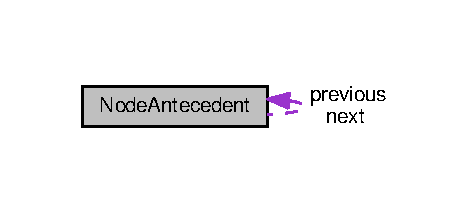
\includegraphics[width=226pt]{struct_node_antecedent__coll__graph}
\end{center}
\end{figure}
\subsection*{Champs de données}
\begin{DoxyCompactItemize}
\item 
char $\ast$ \hyperlink{struct_node_antecedent_a0c3929ebda710960d6b68a88c77f2254}{ante}
\item 
\hyperlink{struct_node_antecedent}{Node\-Antecedent} $\ast$ \hyperlink{struct_node_antecedent_a92d57ada68813cf417c5471a1458927a}{previous}
\item 
\hyperlink{struct_node_antecedent}{Node\-Antecedent} $\ast$ \hyperlink{struct_node_antecedent_a8273a14f46fbc8204294f8db5e3ea9e6}{next}
\end{DoxyCompactItemize}


\subsection{Documentation des champs}
\hypertarget{struct_node_antecedent_a0c3929ebda710960d6b68a88c77f2254}{\index{Node\-Antecedent@{Node\-Antecedent}!ante@{ante}}
\index{ante@{ante}!NodeAntecedent@{Node\-Antecedent}}
\subsubsection[{ante}]{\setlength{\rightskip}{0pt plus 5cm}char$\ast$ ante}}\label{struct_node_antecedent_a0c3929ebda710960d6b68a88c77f2254}
\hypertarget{struct_node_antecedent_a8273a14f46fbc8204294f8db5e3ea9e6}{\index{Node\-Antecedent@{Node\-Antecedent}!next@{next}}
\index{next@{next}!NodeAntecedent@{Node\-Antecedent}}
\subsubsection[{next}]{\setlength{\rightskip}{0pt plus 5cm}{\bf Node\-Antecedent}$\ast$ next}}\label{struct_node_antecedent_a8273a14f46fbc8204294f8db5e3ea9e6}
\hypertarget{struct_node_antecedent_a92d57ada68813cf417c5471a1458927a}{\index{Node\-Antecedent@{Node\-Antecedent}!previous@{previous}}
\index{previous@{previous}!NodeAntecedent@{Node\-Antecedent}}
\subsubsection[{previous}]{\setlength{\rightskip}{0pt plus 5cm}{\bf Node\-Antecedent}$\ast$ previous}}\label{struct_node_antecedent_a92d57ada68813cf417c5471a1458927a}


La documentation de cette structure a été générée à partir du fichier suivant \-:\begin{DoxyCompactItemize}
\item 
include/\-G\-P\-Calendar/\-Model/\hyperlink{dossier__medical_8h}{dossier\-\_\-medical.\-h}\end{DoxyCompactItemize}

\hypertarget{struct_node_jour}{\section{Référence de la structure Node\-Jour}
\label{struct_node_jour}\index{Node\-Jour@{Node\-Jour}}
}


{\ttfamily \#include $<$calendrier.\-h$>$}



Graphe de collaboration de Node\-Jour\-:
\nopagebreak
\begin{figure}[H]
\begin{center}
\leavevmode
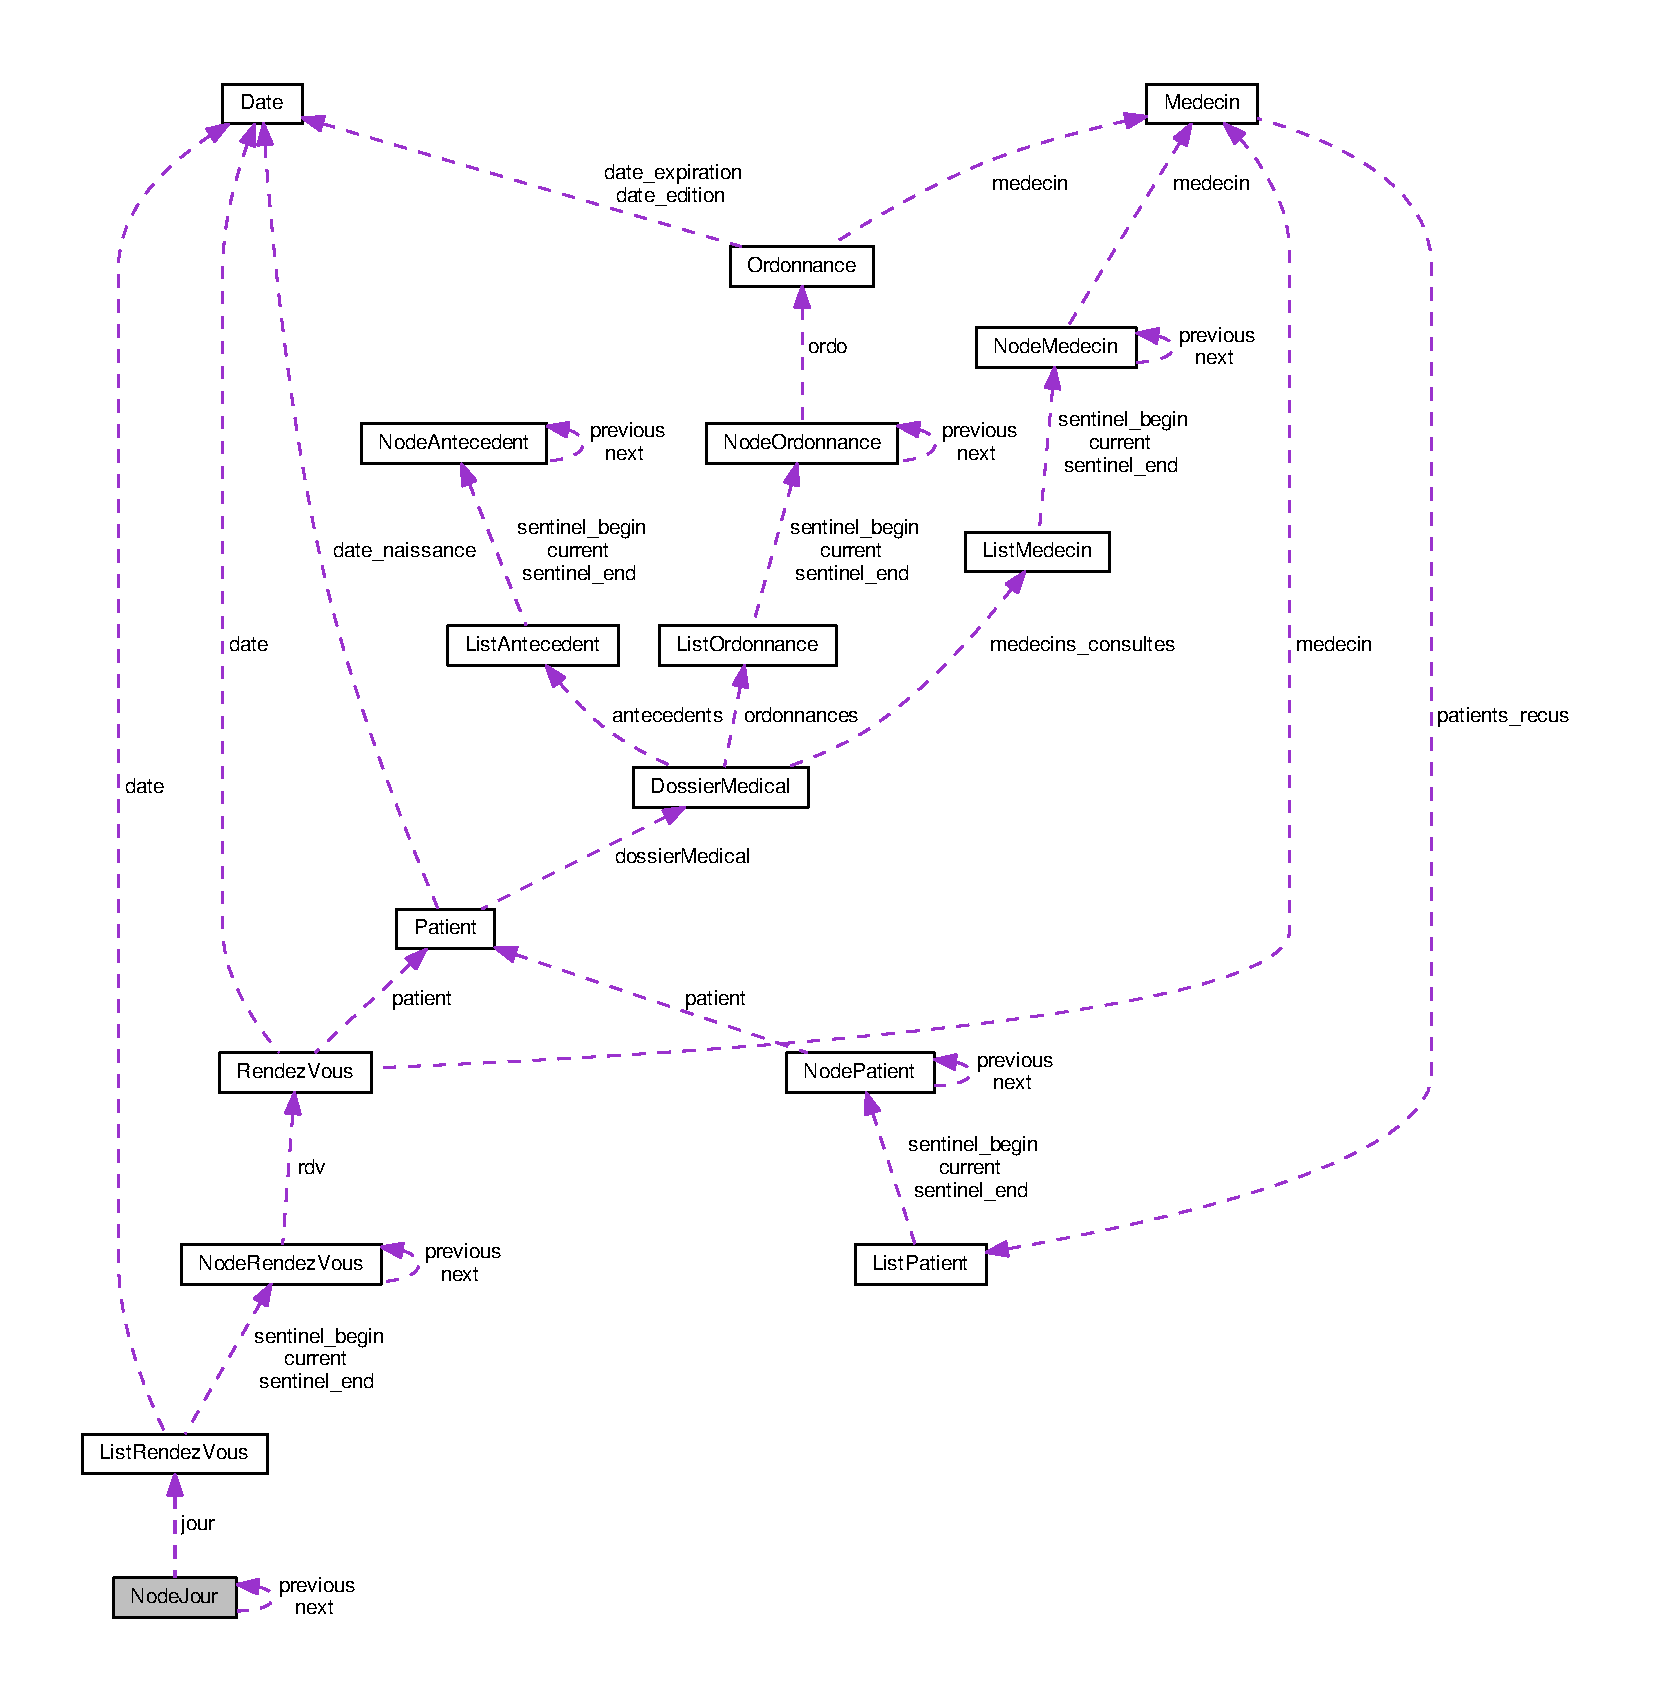
\includegraphics[width=350pt]{struct_node_jour__coll__graph}
\end{center}
\end{figure}
\subsection*{Champs de données}
\begin{DoxyCompactItemize}
\item 
\hyperlink{calendrier_8h_a99e50633bb5c551d09693a390acd33d1}{Jour} \hyperlink{struct_node_jour_a6b700af15ea48800affa955a00734b02}{jour}
\item 
struct \hyperlink{struct_node_jour}{Node\-Jour} $\ast$ \hyperlink{struct_node_jour_a4d4c1312d6c41b196a1eca69e533f9b3}{next}
\item 
struct \hyperlink{struct_node_jour}{Node\-Jour} $\ast$ \hyperlink{struct_node_jour_acaf7d4f45774acfb09a39e336ebd1af7}{previous}
\end{DoxyCompactItemize}


\subsection{Documentation des champs}
\hypertarget{struct_node_jour_a6b700af15ea48800affa955a00734b02}{\index{Node\-Jour@{Node\-Jour}!jour@{jour}}
\index{jour@{jour}!NodeJour@{Node\-Jour}}
\subsubsection[{jour}]{\setlength{\rightskip}{0pt plus 5cm}{\bf Jour} jour}}\label{struct_node_jour_a6b700af15ea48800affa955a00734b02}
\hypertarget{struct_node_jour_a4d4c1312d6c41b196a1eca69e533f9b3}{\index{Node\-Jour@{Node\-Jour}!next@{next}}
\index{next@{next}!NodeJour@{Node\-Jour}}
\subsubsection[{next}]{\setlength{\rightskip}{0pt plus 5cm}struct {\bf Node\-Jour}$\ast$ next}}\label{struct_node_jour_a4d4c1312d6c41b196a1eca69e533f9b3}
\hypertarget{struct_node_jour_acaf7d4f45774acfb09a39e336ebd1af7}{\index{Node\-Jour@{Node\-Jour}!previous@{previous}}
\index{previous@{previous}!NodeJour@{Node\-Jour}}
\subsubsection[{previous}]{\setlength{\rightskip}{0pt plus 5cm}struct {\bf Node\-Jour}$\ast$ previous}}\label{struct_node_jour_acaf7d4f45774acfb09a39e336ebd1af7}


La documentation de cette structure a été générée à partir du fichier suivant \-:\begin{DoxyCompactItemize}
\item 
include/\-G\-P\-Calendar/\-Model/\hyperlink{calendrier_8h}{calendrier.\-h}\end{DoxyCompactItemize}

\hypertarget{struct_node_medecin}{\section{Référence de la structure Node\-Medecin}
\label{struct_node_medecin}\index{Node\-Medecin@{Node\-Medecin}}
}


{\ttfamily \#include $<$medecin.\-h$>$}



Graphe de collaboration de Node\-Medecin\-:
\nopagebreak
\begin{figure}[H]
\begin{center}
\leavevmode
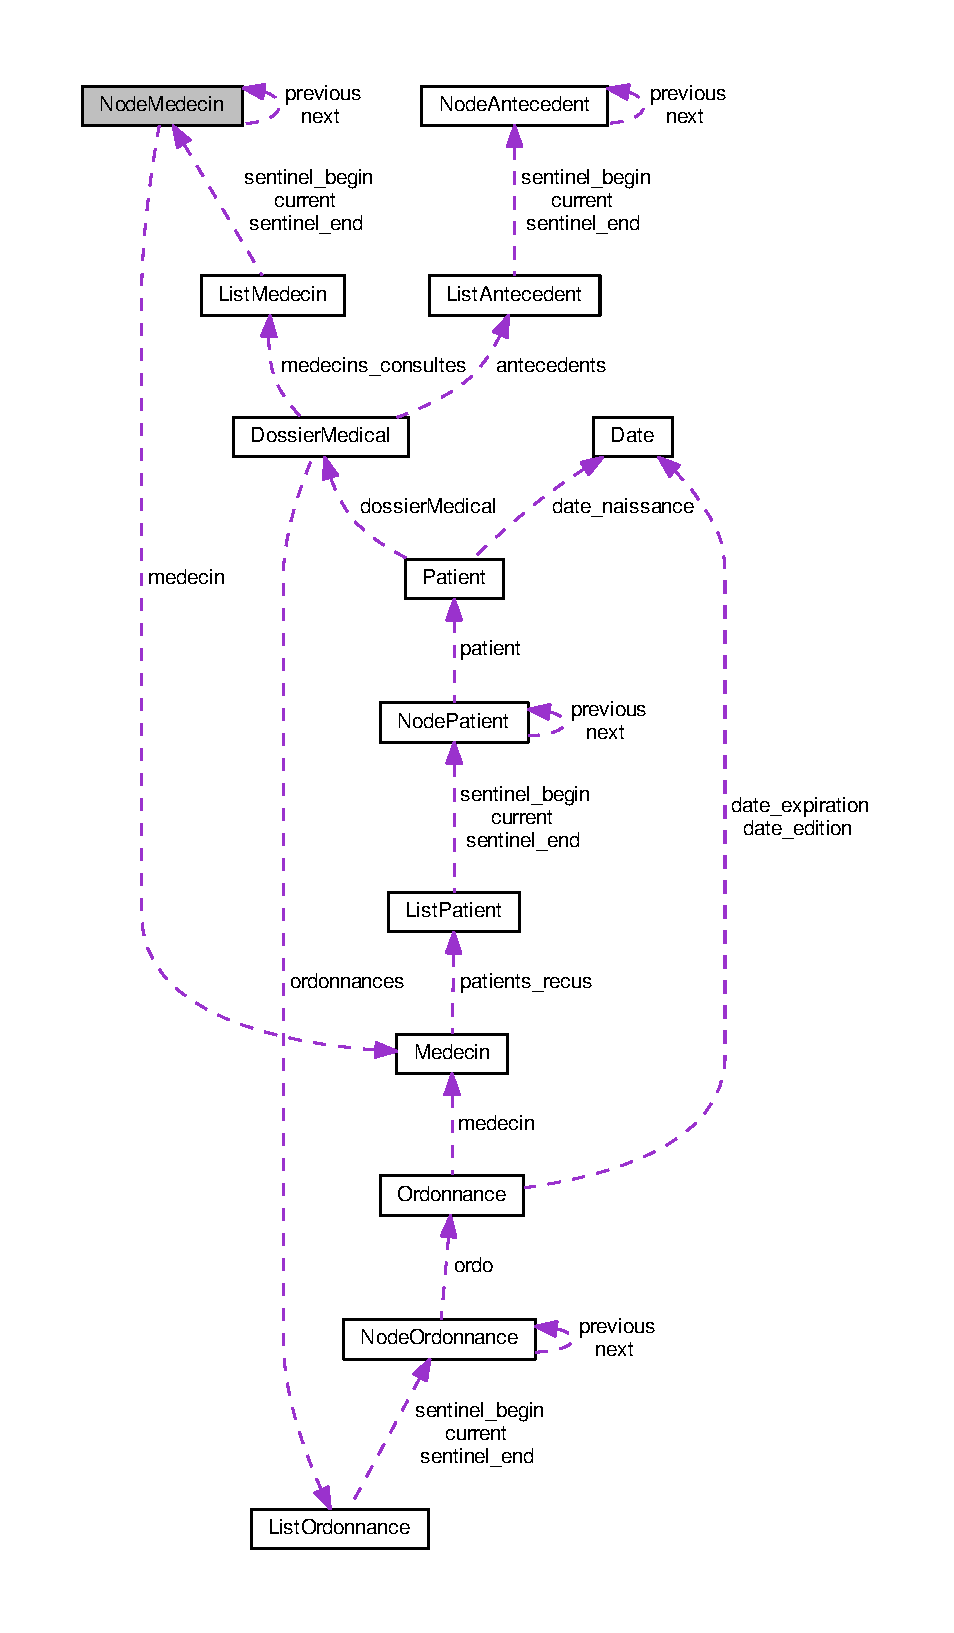
\includegraphics[height=550pt]{struct_node_medecin__coll__graph}
\end{center}
\end{figure}
\subsection*{Champs de données}
\begin{DoxyCompactItemize}
\item 
\hyperlink{struct_medecin}{Medecin} $\ast$ \hyperlink{struct_node_medecin_a59131973441fcf6250df021bcf96d17c}{medecin}
\item 
struct \hyperlink{struct_node_medecin}{Node\-Medecin} $\ast$ \hyperlink{struct_node_medecin_a0cbe061047b7421412bf7e7dfc5b14f6}{previous}
\item 
struct \hyperlink{struct_node_medecin}{Node\-Medecin} $\ast$ \hyperlink{struct_node_medecin_a2bccf75b1d4b377994dcbb49ebdb9207}{next}
\end{DoxyCompactItemize}


\subsection{Documentation des champs}
\hypertarget{struct_node_medecin_a59131973441fcf6250df021bcf96d17c}{\index{Node\-Medecin@{Node\-Medecin}!medecin@{medecin}}
\index{medecin@{medecin}!NodeMedecin@{Node\-Medecin}}
\subsubsection[{medecin}]{\setlength{\rightskip}{0pt plus 5cm}{\bf Medecin}$\ast$ medecin}}\label{struct_node_medecin_a59131973441fcf6250df021bcf96d17c}
\hypertarget{struct_node_medecin_a2bccf75b1d4b377994dcbb49ebdb9207}{\index{Node\-Medecin@{Node\-Medecin}!next@{next}}
\index{next@{next}!NodeMedecin@{Node\-Medecin}}
\subsubsection[{next}]{\setlength{\rightskip}{0pt plus 5cm}struct {\bf Node\-Medecin}$\ast$ next}}\label{struct_node_medecin_a2bccf75b1d4b377994dcbb49ebdb9207}
\hypertarget{struct_node_medecin_a0cbe061047b7421412bf7e7dfc5b14f6}{\index{Node\-Medecin@{Node\-Medecin}!previous@{previous}}
\index{previous@{previous}!NodeMedecin@{Node\-Medecin}}
\subsubsection[{previous}]{\setlength{\rightskip}{0pt plus 5cm}struct {\bf Node\-Medecin}$\ast$ previous}}\label{struct_node_medecin_a0cbe061047b7421412bf7e7dfc5b14f6}


La documentation de cette structure a été générée à partir du fichier suivant \-:\begin{DoxyCompactItemize}
\item 
include/\-G\-P\-Calendar/\-Model/\hyperlink{medecin_8h}{medecin.\-h}\end{DoxyCompactItemize}

\hypertarget{struct_node_mois}{\section{Référence de la structure Node\-Mois}
\label{struct_node_mois}\index{Node\-Mois@{Node\-Mois}}
}


{\ttfamily \#include $<$calendrier.\-h$>$}



Graphe de collaboration de Node\-Mois\-:
\nopagebreak
\begin{figure}[H]
\begin{center}
\leavevmode
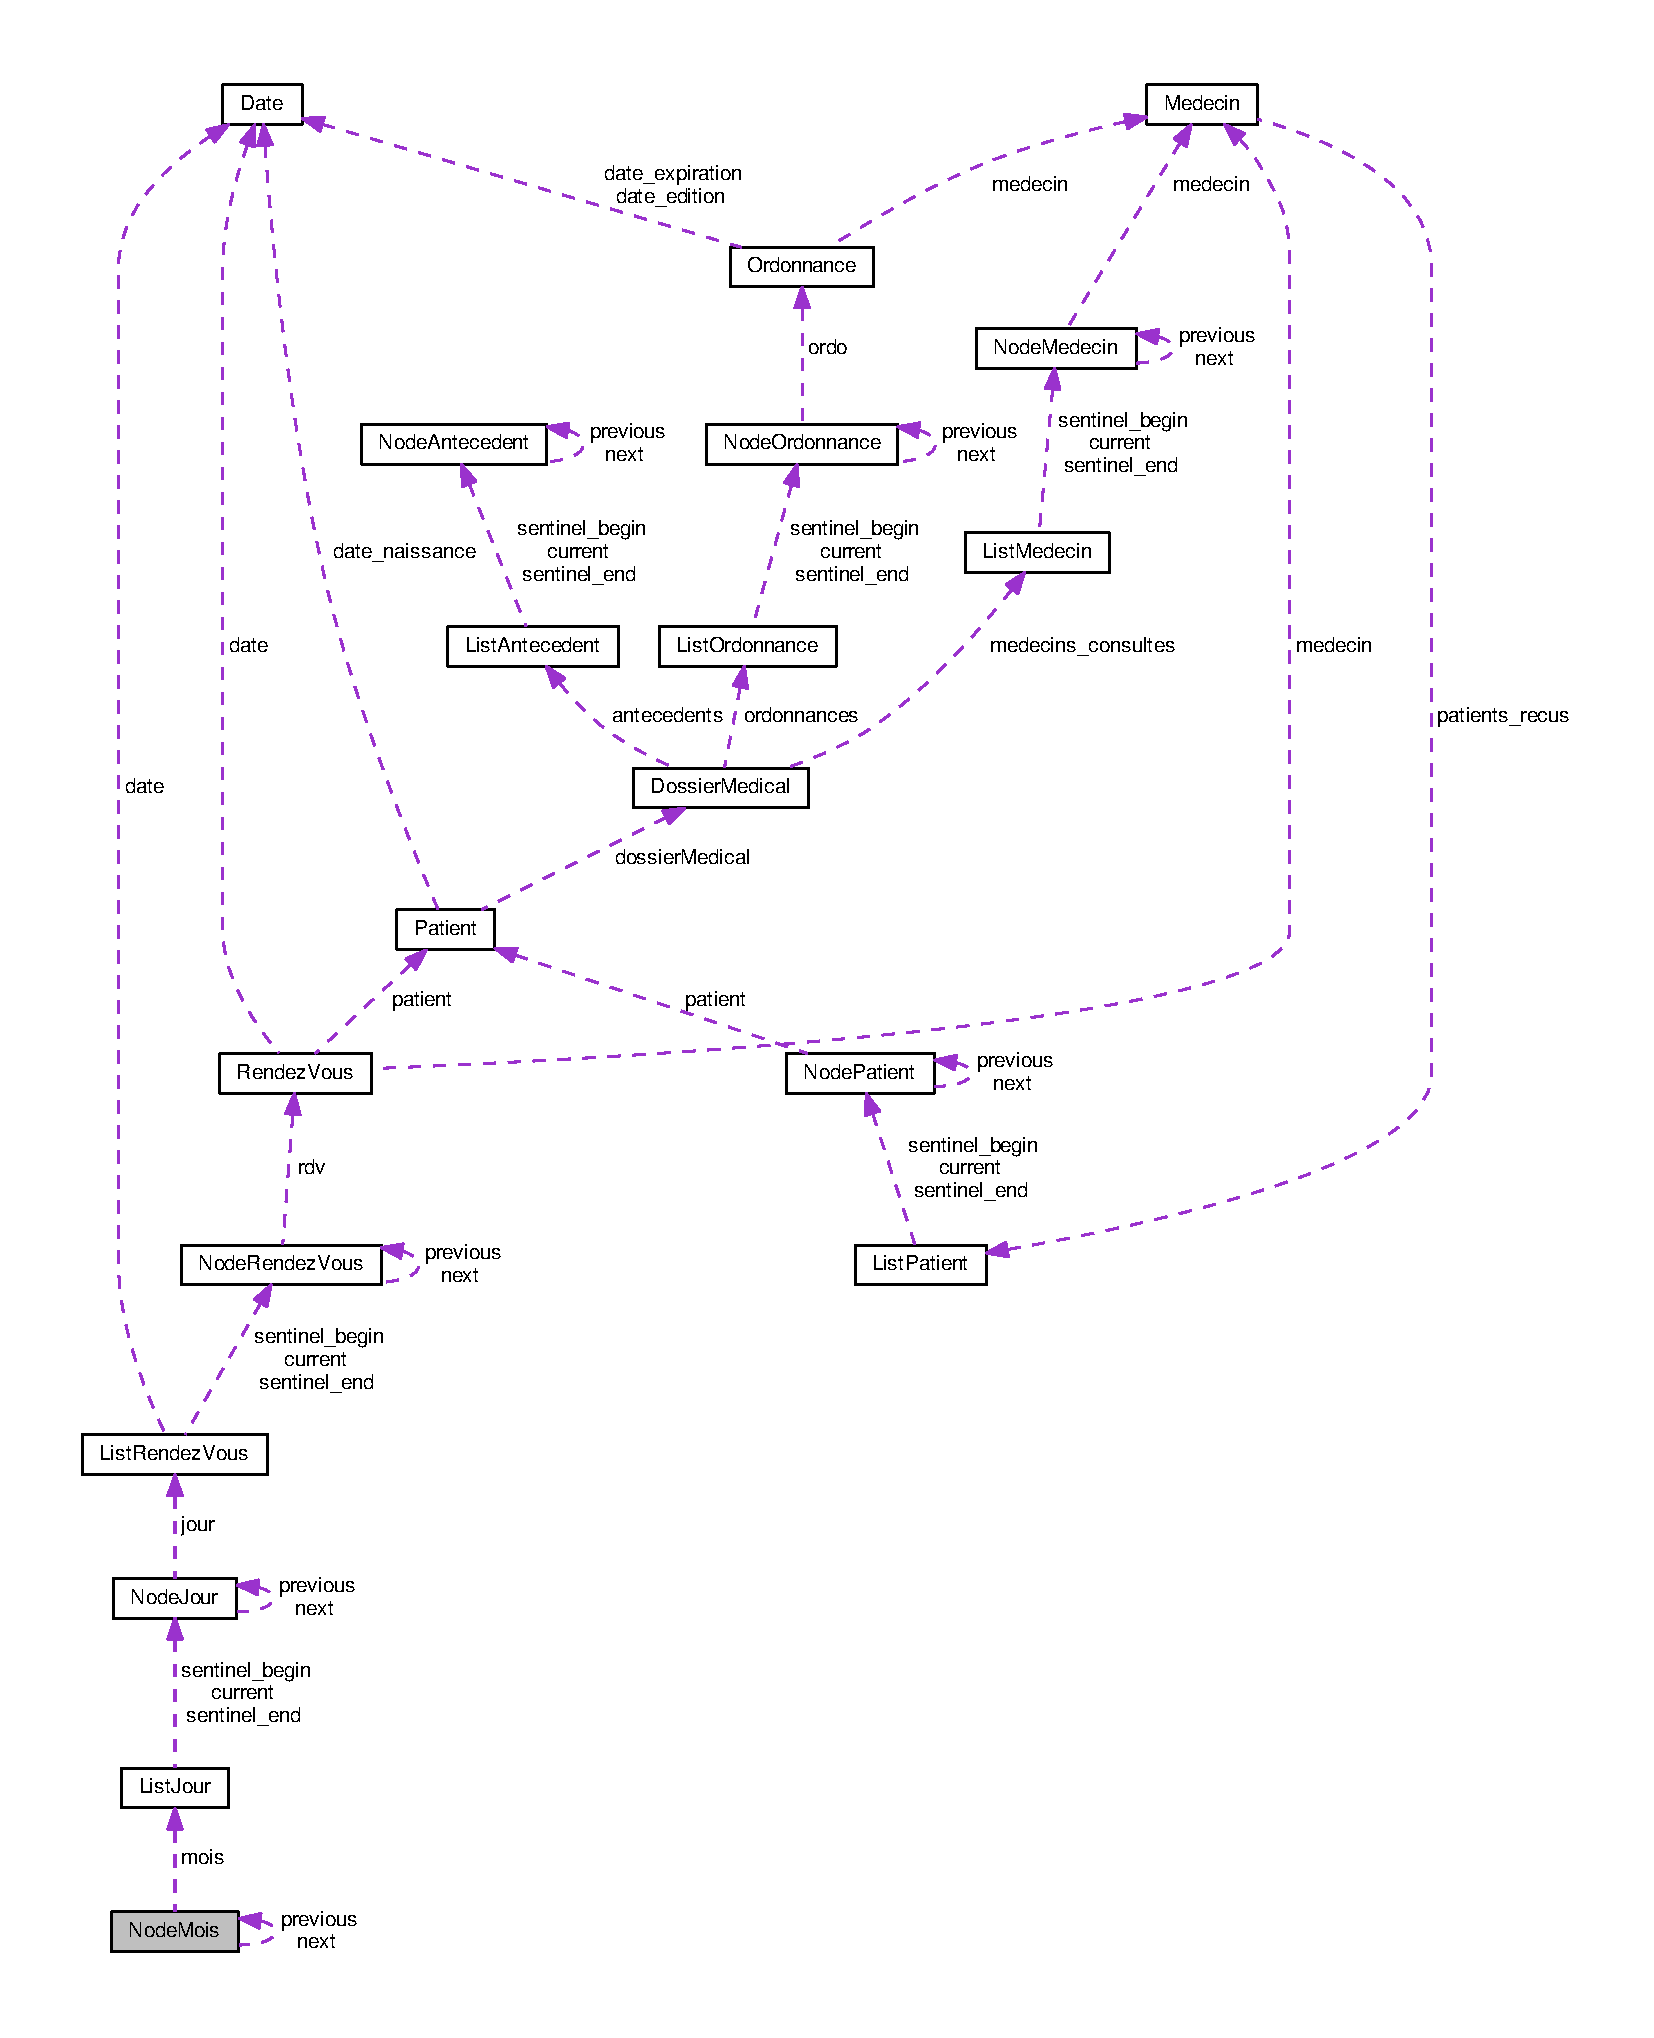
\includegraphics[width=350pt]{struct_node_mois__coll__graph}
\end{center}
\end{figure}
\subsection*{Champs de données}
\begin{DoxyCompactItemize}
\item 
\hyperlink{calendrier_8h_ae3a97c3f15c38f94baef498c511b4258}{Mois} \hyperlink{struct_node_mois_ab849c15d22d8cdd9c32d94bfc37033eb}{mois}
\item 
struct \hyperlink{struct_node_mois}{Node\-Mois} $\ast$ \hyperlink{struct_node_mois_a91a0a35c8966de2862bf897c1c914b3e}{next}
\item 
struct \hyperlink{struct_node_mois}{Node\-Mois} $\ast$ \hyperlink{struct_node_mois_a9c424087093e46294bf21e09595ca6e0}{previous}
\end{DoxyCompactItemize}


\subsection{Documentation des champs}
\hypertarget{struct_node_mois_ab849c15d22d8cdd9c32d94bfc37033eb}{\index{Node\-Mois@{Node\-Mois}!mois@{mois}}
\index{mois@{mois}!NodeMois@{Node\-Mois}}
\subsubsection[{mois}]{\setlength{\rightskip}{0pt plus 5cm}{\bf Mois} mois}}\label{struct_node_mois_ab849c15d22d8cdd9c32d94bfc37033eb}
\hypertarget{struct_node_mois_a91a0a35c8966de2862bf897c1c914b3e}{\index{Node\-Mois@{Node\-Mois}!next@{next}}
\index{next@{next}!NodeMois@{Node\-Mois}}
\subsubsection[{next}]{\setlength{\rightskip}{0pt plus 5cm}struct {\bf Node\-Mois}$\ast$ next}}\label{struct_node_mois_a91a0a35c8966de2862bf897c1c914b3e}
\hypertarget{struct_node_mois_a9c424087093e46294bf21e09595ca6e0}{\index{Node\-Mois@{Node\-Mois}!previous@{previous}}
\index{previous@{previous}!NodeMois@{Node\-Mois}}
\subsubsection[{previous}]{\setlength{\rightskip}{0pt plus 5cm}struct {\bf Node\-Mois}$\ast$ previous}}\label{struct_node_mois_a9c424087093e46294bf21e09595ca6e0}


La documentation de cette structure a été générée à partir du fichier suivant \-:\begin{DoxyCompactItemize}
\item 
include/\-G\-P\-Calendar/\-Model/\hyperlink{calendrier_8h}{calendrier.\-h}\end{DoxyCompactItemize}

\hypertarget{struct_node_ordonnance}{\section{Référence de la structure Node\-Ordonnance}
\label{struct_node_ordonnance}\index{Node\-Ordonnance@{Node\-Ordonnance}}
}


{\ttfamily \#include $<$ordonnance.\-h$>$}



Graphe de collaboration de Node\-Ordonnance\-:
\nopagebreak
\begin{figure}[H]
\begin{center}
\leavevmode
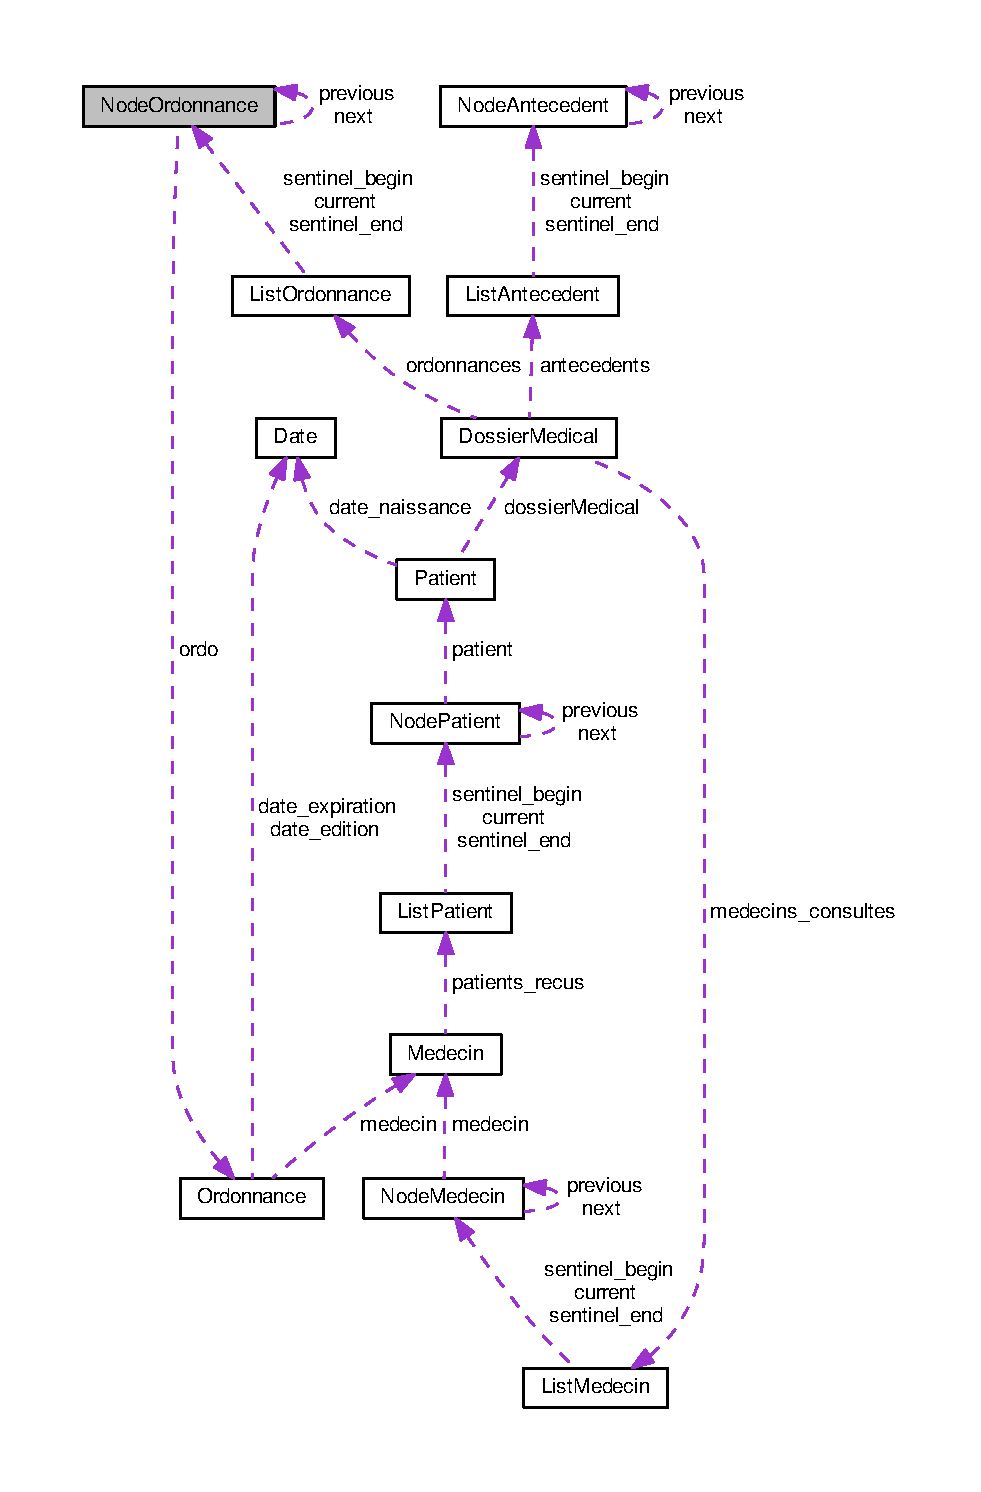
\includegraphics[width=350pt]{struct_node_ordonnance__coll__graph}
\end{center}
\end{figure}
\subsection*{Champs de données}
\begin{DoxyCompactItemize}
\item 
\hyperlink{struct_ordonnance}{Ordonnance} $\ast$ \hyperlink{struct_node_ordonnance_ad6081216f8df13cefec2383c92776b3e}{ordo}
\item 
\hyperlink{struct_node_ordonnance}{Node\-Ordonnance} $\ast$ \hyperlink{struct_node_ordonnance_a3ea5580d83870a88946801967c6940be}{previous}
\item 
\hyperlink{struct_node_ordonnance}{Node\-Ordonnance} $\ast$ \hyperlink{struct_node_ordonnance_a7b34255519f5fe256a0ad0979680e632}{next}
\end{DoxyCompactItemize}


\subsection{Documentation des champs}
\hypertarget{struct_node_ordonnance_a7b34255519f5fe256a0ad0979680e632}{\index{Node\-Ordonnance@{Node\-Ordonnance}!next@{next}}
\index{next@{next}!NodeOrdonnance@{Node\-Ordonnance}}
\subsubsection[{next}]{\setlength{\rightskip}{0pt plus 5cm}{\bf Node\-Ordonnance}$\ast$ next}}\label{struct_node_ordonnance_a7b34255519f5fe256a0ad0979680e632}
\hypertarget{struct_node_ordonnance_ad6081216f8df13cefec2383c92776b3e}{\index{Node\-Ordonnance@{Node\-Ordonnance}!ordo@{ordo}}
\index{ordo@{ordo}!NodeOrdonnance@{Node\-Ordonnance}}
\subsubsection[{ordo}]{\setlength{\rightskip}{0pt plus 5cm}{\bf Ordonnance}$\ast$ ordo}}\label{struct_node_ordonnance_ad6081216f8df13cefec2383c92776b3e}
\hypertarget{struct_node_ordonnance_a3ea5580d83870a88946801967c6940be}{\index{Node\-Ordonnance@{Node\-Ordonnance}!previous@{previous}}
\index{previous@{previous}!NodeOrdonnance@{Node\-Ordonnance}}
\subsubsection[{previous}]{\setlength{\rightskip}{0pt plus 5cm}{\bf Node\-Ordonnance}$\ast$ previous}}\label{struct_node_ordonnance_a3ea5580d83870a88946801967c6940be}


La documentation de cette structure a été générée à partir du fichier suivant \-:\begin{DoxyCompactItemize}
\item 
include/\-G\-P\-Calendar/\-Model/\hyperlink{ordonnance_8h}{ordonnance.\-h}\end{DoxyCompactItemize}

\hypertarget{struct_node_patient}{\section{Référence de la structure Node\-Patient}
\label{struct_node_patient}\index{Node\-Patient@{Node\-Patient}}
}


{\ttfamily \#include $<$patient.\-h$>$}



Graphe de collaboration de Node\-Patient\-:
\nopagebreak
\begin{figure}[H]
\begin{center}
\leavevmode
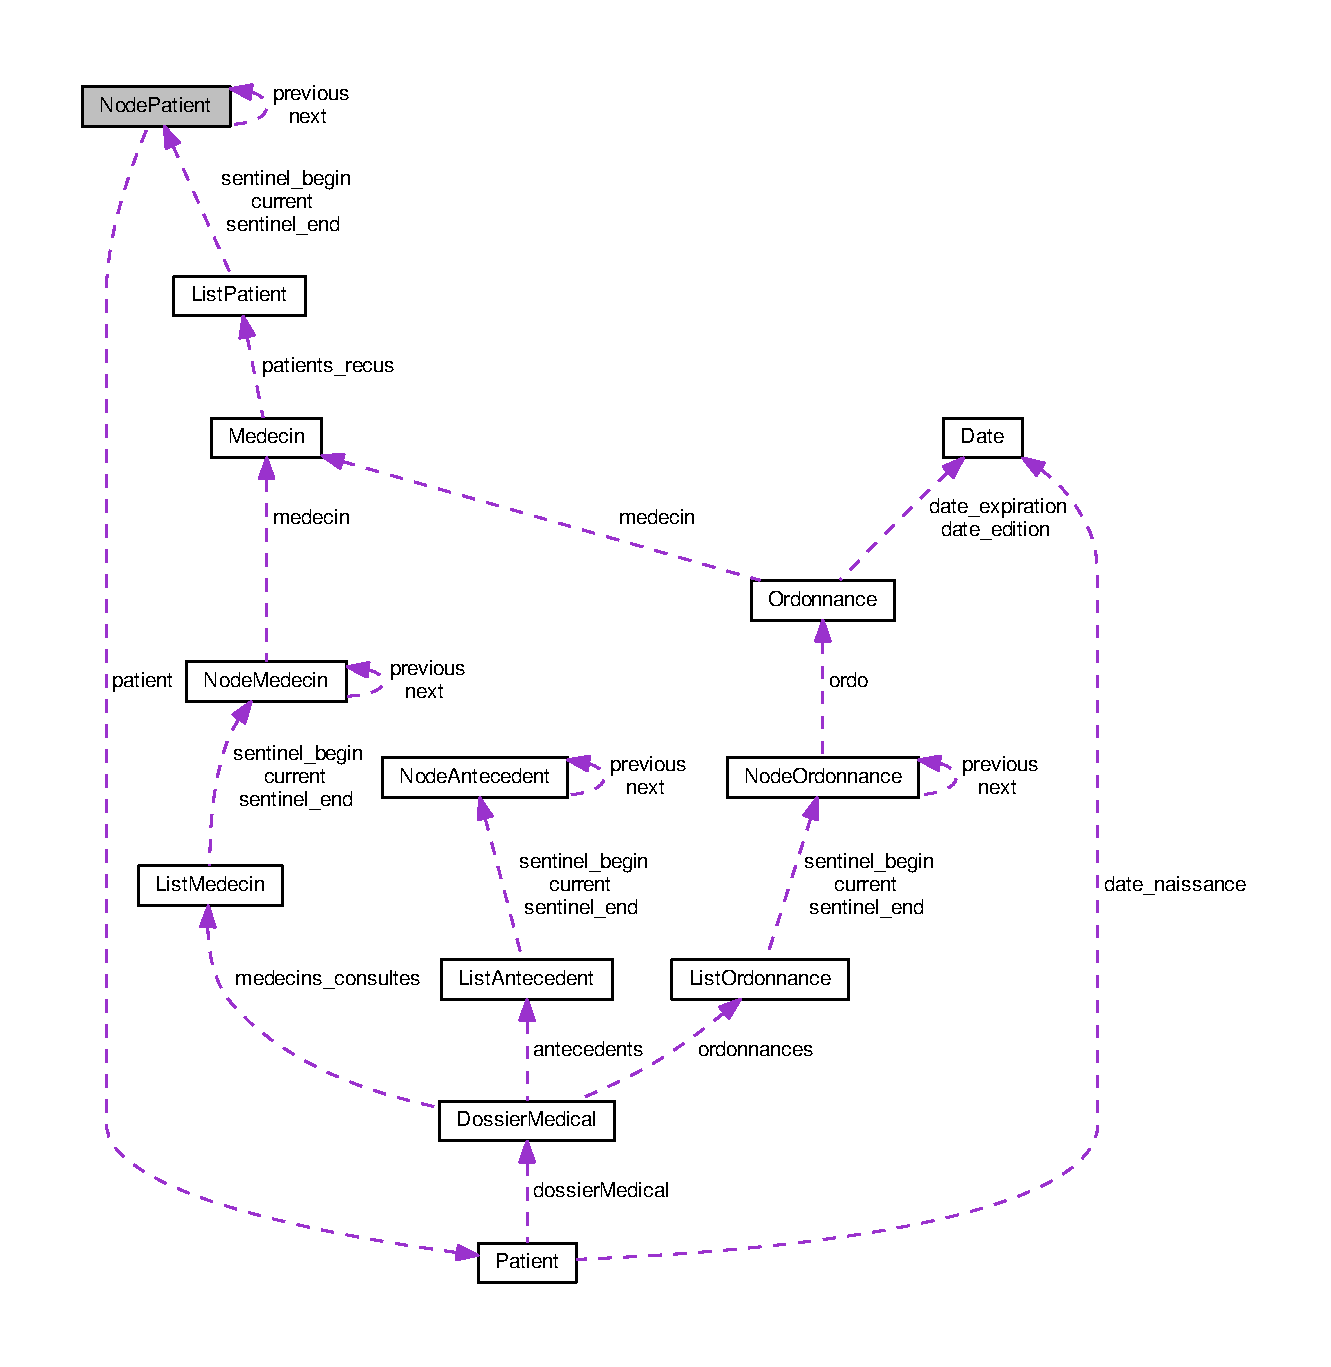
\includegraphics[width=350pt]{struct_node_patient__coll__graph}
\end{center}
\end{figure}
\subsection*{Champs de données}
\begin{DoxyCompactItemize}
\item 
\hyperlink{struct_patient}{Patient} $\ast$ \hyperlink{struct_node_patient_a602d93e6dfbb9a54fc31419f2463ac2b}{patient}
\item 
struct \hyperlink{struct_node_patient}{Node\-Patient} $\ast$ \hyperlink{struct_node_patient_ad96b030b2d205d958d0119a33cd84723}{previous}
\item 
struct \hyperlink{struct_node_patient}{Node\-Patient} $\ast$ \hyperlink{struct_node_patient_aed83e2f44d9cd8414c6dceebd6e34f40}{next}
\end{DoxyCompactItemize}


\subsection{Documentation des champs}
\hypertarget{struct_node_patient_aed83e2f44d9cd8414c6dceebd6e34f40}{\index{Node\-Patient@{Node\-Patient}!next@{next}}
\index{next@{next}!NodePatient@{Node\-Patient}}
\subsubsection[{next}]{\setlength{\rightskip}{0pt plus 5cm}struct {\bf Node\-Patient}$\ast$ next}}\label{struct_node_patient_aed83e2f44d9cd8414c6dceebd6e34f40}
\hypertarget{struct_node_patient_a602d93e6dfbb9a54fc31419f2463ac2b}{\index{Node\-Patient@{Node\-Patient}!patient@{patient}}
\index{patient@{patient}!NodePatient@{Node\-Patient}}
\subsubsection[{patient}]{\setlength{\rightskip}{0pt plus 5cm}{\bf Patient}$\ast$ patient}}\label{struct_node_patient_a602d93e6dfbb9a54fc31419f2463ac2b}
\hypertarget{struct_node_patient_ad96b030b2d205d958d0119a33cd84723}{\index{Node\-Patient@{Node\-Patient}!previous@{previous}}
\index{previous@{previous}!NodePatient@{Node\-Patient}}
\subsubsection[{previous}]{\setlength{\rightskip}{0pt plus 5cm}struct {\bf Node\-Patient}$\ast$ previous}}\label{struct_node_patient_ad96b030b2d205d958d0119a33cd84723}


La documentation de cette structure a été générée à partir du fichier suivant \-:\begin{DoxyCompactItemize}
\item 
include/\-G\-P\-Calendar/\-Model/\hyperlink{patient_8h}{patient.\-h}\end{DoxyCompactItemize}

\hypertarget{struct_node_rendez_vous}{\section{Référence de la structure Node\-Rendez\-Vous}
\label{struct_node_rendez_vous}\index{Node\-Rendez\-Vous@{Node\-Rendez\-Vous}}
}


{\ttfamily \#include $<$calendrier.\-h$>$}



Graphe de collaboration de Node\-Rendez\-Vous\-:
\nopagebreak
\begin{figure}[H]
\begin{center}
\leavevmode
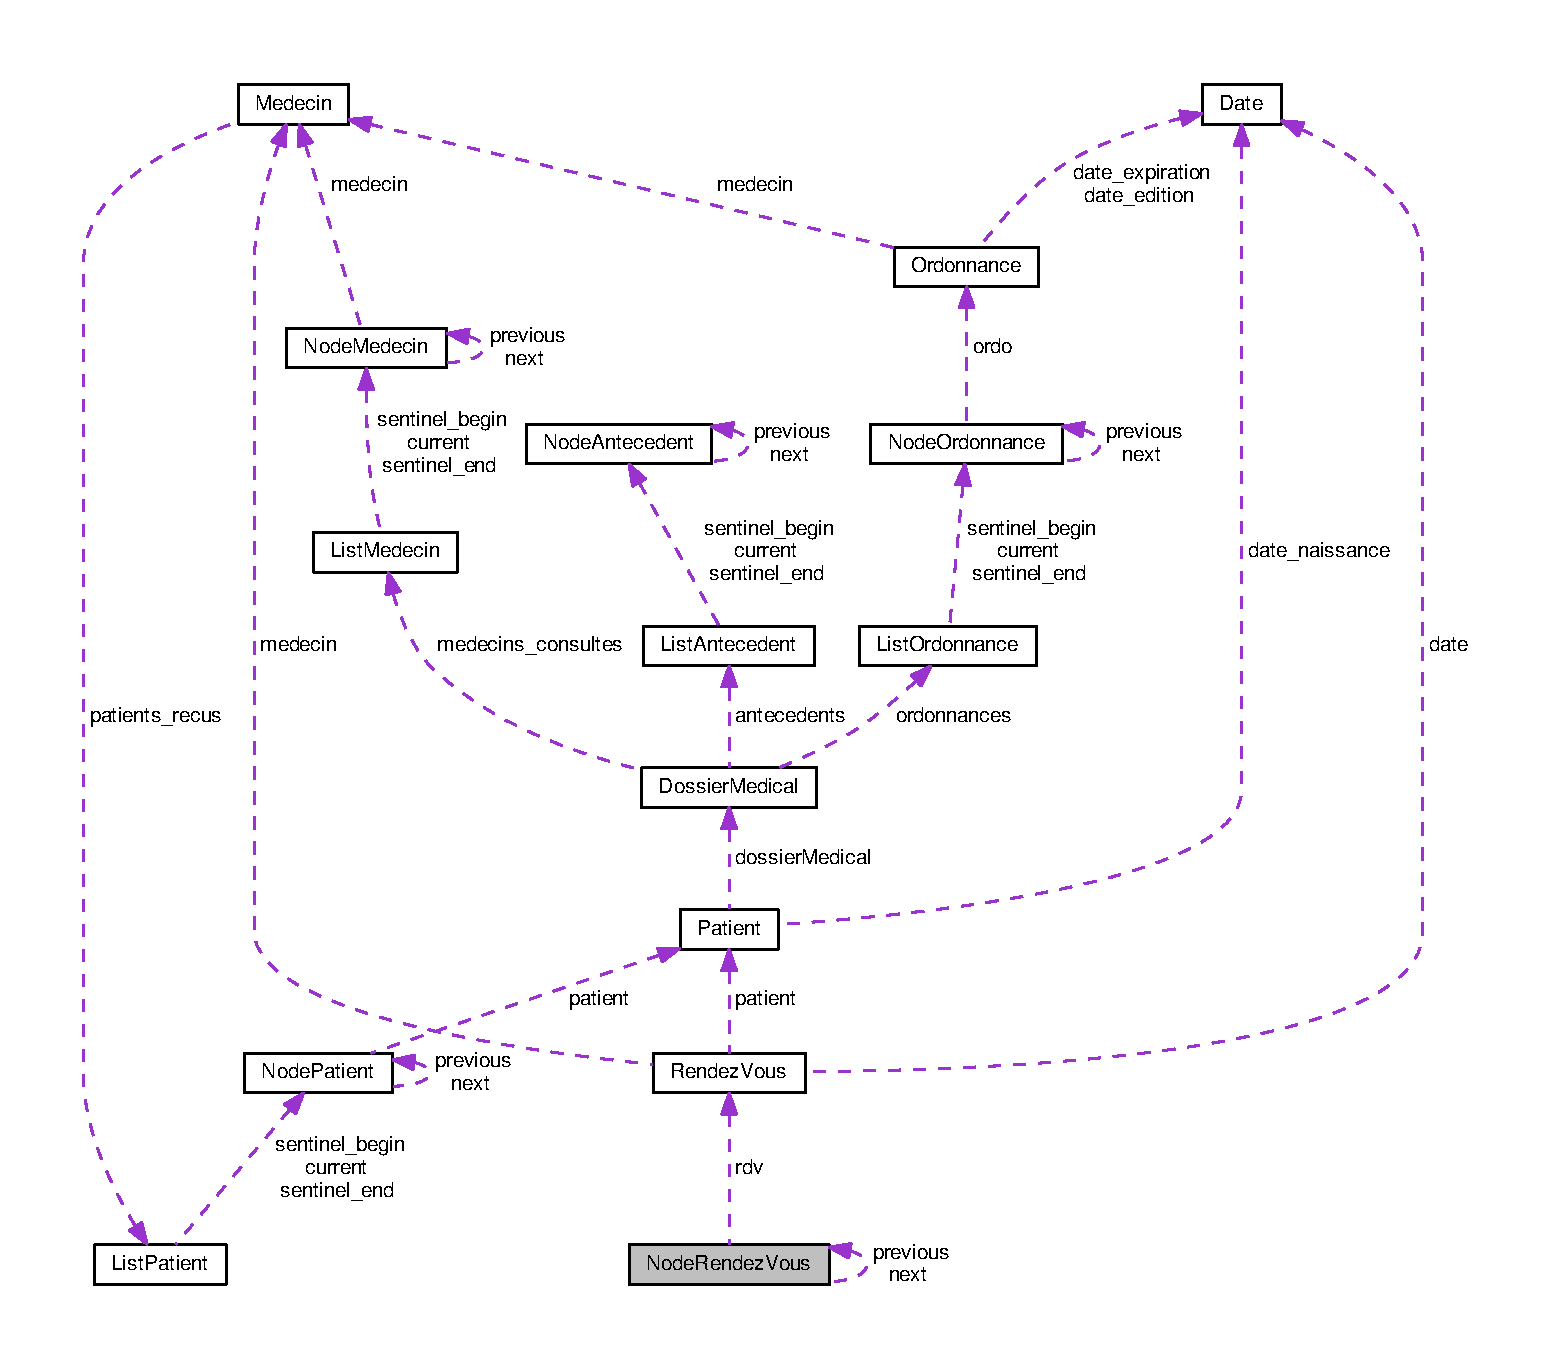
\includegraphics[width=350pt]{struct_node_rendez_vous__coll__graph}
\end{center}
\end{figure}
\subsection*{Champs de données}
\begin{DoxyCompactItemize}
\item 
\hyperlink{struct_rendez_vous}{Rendez\-Vous} $\ast$ \hyperlink{struct_node_rendez_vous_af79db64558cdbcd5406072274edcc1b5}{rdv}
\item 
\hyperlink{struct_node_rendez_vous}{Node\-Rendez\-Vous} $\ast$ \hyperlink{struct_node_rendez_vous_a84662a2ba345d017dd59a013b040e53e}{next}
\item 
\hyperlink{struct_node_rendez_vous}{Node\-Rendez\-Vous} $\ast$ \hyperlink{struct_node_rendez_vous_ab9f2e3f151f5b84ed16f14e554374470}{previous}
\end{DoxyCompactItemize}


\subsection{Documentation des champs}
\hypertarget{struct_node_rendez_vous_a84662a2ba345d017dd59a013b040e53e}{\index{Node\-Rendez\-Vous@{Node\-Rendez\-Vous}!next@{next}}
\index{next@{next}!NodeRendezVous@{Node\-Rendez\-Vous}}
\subsubsection[{next}]{\setlength{\rightskip}{0pt plus 5cm}{\bf Node\-Rendez\-Vous}$\ast$ next}}\label{struct_node_rendez_vous_a84662a2ba345d017dd59a013b040e53e}
\hypertarget{struct_node_rendez_vous_ab9f2e3f151f5b84ed16f14e554374470}{\index{Node\-Rendez\-Vous@{Node\-Rendez\-Vous}!previous@{previous}}
\index{previous@{previous}!NodeRendezVous@{Node\-Rendez\-Vous}}
\subsubsection[{previous}]{\setlength{\rightskip}{0pt plus 5cm}{\bf Node\-Rendez\-Vous}$\ast$ previous}}\label{struct_node_rendez_vous_ab9f2e3f151f5b84ed16f14e554374470}
\hypertarget{struct_node_rendez_vous_af79db64558cdbcd5406072274edcc1b5}{\index{Node\-Rendez\-Vous@{Node\-Rendez\-Vous}!rdv@{rdv}}
\index{rdv@{rdv}!NodeRendezVous@{Node\-Rendez\-Vous}}
\subsubsection[{rdv}]{\setlength{\rightskip}{0pt plus 5cm}{\bf Rendez\-Vous}$\ast$ rdv}}\label{struct_node_rendez_vous_af79db64558cdbcd5406072274edcc1b5}


La documentation de cette structure a été générée à partir du fichier suivant \-:\begin{DoxyCompactItemize}
\item 
include/\-G\-P\-Calendar/\-Model/\hyperlink{calendrier_8h}{calendrier.\-h}\end{DoxyCompactItemize}

\hypertarget{struct_ordonnance}{\section{Référence de la structure Ordonnance}
\label{struct_ordonnance}\index{Ordonnance@{Ordonnance}}
}


{\ttfamily \#include $<$ordonnance.\-h$>$}



Graphe de collaboration de Ordonnance\-:
\nopagebreak
\begin{figure}[H]
\begin{center}
\leavevmode
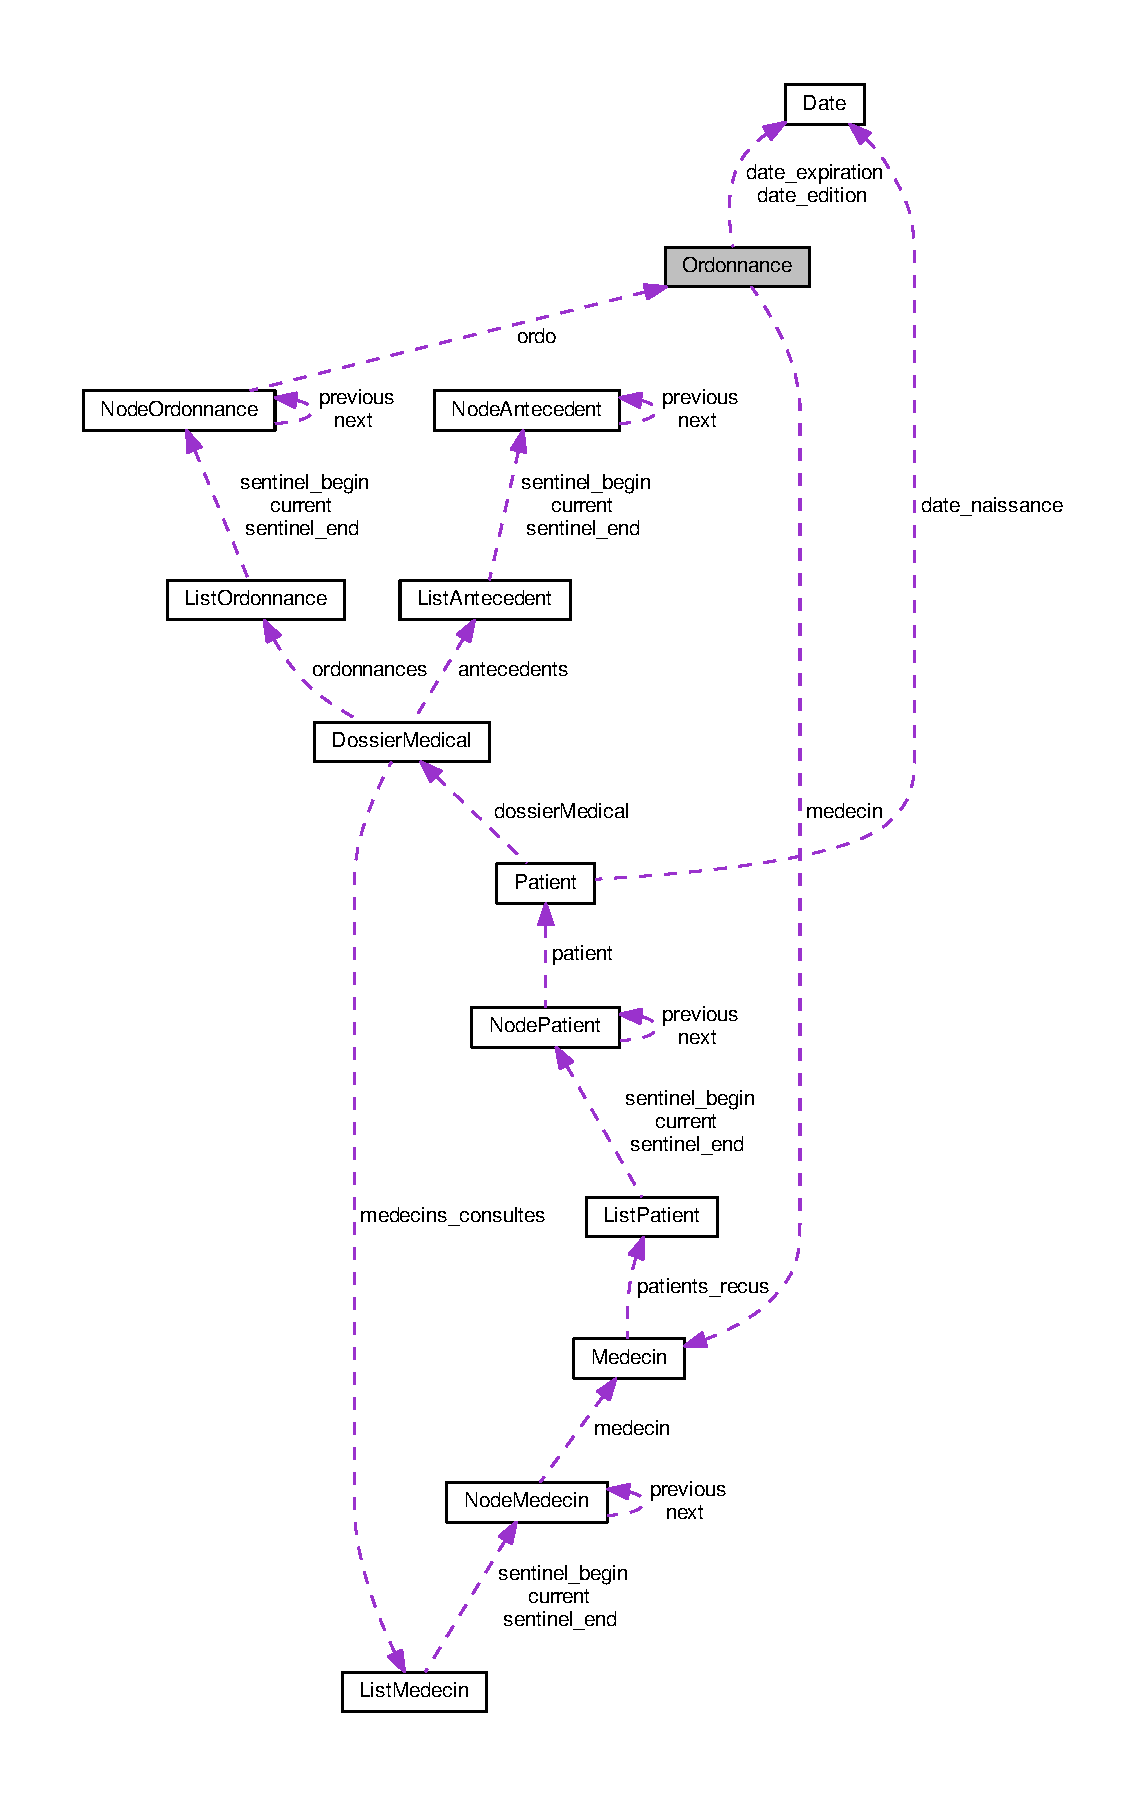
\includegraphics[width=350pt]{struct_ordonnance__coll__graph}
\end{center}
\end{figure}
\subsection*{Champs de données}
\begin{DoxyCompactItemize}
\item 
\hyperlink{struct_medecin}{Medecin} $\ast$ \hyperlink{struct_ordonnance_a59131973441fcf6250df021bcf96d17c}{medecin}
\item 
\hyperlink{struct_date}{Date} $\ast$ \hyperlink{struct_ordonnance_aa5093841fb5268f587e2ca60b5c3b4ef}{date\-\_\-edition}
\item 
\hyperlink{struct_date}{Date} $\ast$ \hyperlink{struct_ordonnance_aebd9ad8d48f13c9f6271ff87c78f1cb5}{date\-\_\-expiration}
\item 
char $\ast$ \hyperlink{struct_ordonnance_a8444d6e0dfe2bbab0b5e7b24308f1559}{description}
\end{DoxyCompactItemize}


\subsection{Documentation des champs}
\hypertarget{struct_ordonnance_aa5093841fb5268f587e2ca60b5c3b4ef}{\index{Ordonnance@{Ordonnance}!date\-\_\-edition@{date\-\_\-edition}}
\index{date\-\_\-edition@{date\-\_\-edition}!Ordonnance@{Ordonnance}}
\subsubsection[{date\-\_\-edition}]{\setlength{\rightskip}{0pt plus 5cm}{\bf Date}$\ast$ date\-\_\-edition}}\label{struct_ordonnance_aa5093841fb5268f587e2ca60b5c3b4ef}
\hypertarget{struct_ordonnance_aebd9ad8d48f13c9f6271ff87c78f1cb5}{\index{Ordonnance@{Ordonnance}!date\-\_\-expiration@{date\-\_\-expiration}}
\index{date\-\_\-expiration@{date\-\_\-expiration}!Ordonnance@{Ordonnance}}
\subsubsection[{date\-\_\-expiration}]{\setlength{\rightskip}{0pt plus 5cm}{\bf Date}$\ast$ date\-\_\-expiration}}\label{struct_ordonnance_aebd9ad8d48f13c9f6271ff87c78f1cb5}
\hypertarget{struct_ordonnance_a8444d6e0dfe2bbab0b5e7b24308f1559}{\index{Ordonnance@{Ordonnance}!description@{description}}
\index{description@{description}!Ordonnance@{Ordonnance}}
\subsubsection[{description}]{\setlength{\rightskip}{0pt plus 5cm}char$\ast$ description}}\label{struct_ordonnance_a8444d6e0dfe2bbab0b5e7b24308f1559}
\hypertarget{struct_ordonnance_a59131973441fcf6250df021bcf96d17c}{\index{Ordonnance@{Ordonnance}!medecin@{medecin}}
\index{medecin@{medecin}!Ordonnance@{Ordonnance}}
\subsubsection[{medecin}]{\setlength{\rightskip}{0pt plus 5cm}{\bf Medecin}$\ast$ medecin}}\label{struct_ordonnance_a59131973441fcf6250df021bcf96d17c}


La documentation de cette structure a été générée à partir du fichier suivant \-:\begin{DoxyCompactItemize}
\item 
include/\-G\-P\-Calendar/\-Model/\hyperlink{ordonnance_8h}{ordonnance.\-h}\end{DoxyCompactItemize}

\hypertarget{struct_patient}{\section{Référence de la structure Patient}
\label{struct_patient}\index{Patient@{Patient}}
}


{\ttfamily \#include $<$patient.\-h$>$}



Graphe de collaboration de Patient\-:
\nopagebreak
\begin{figure}[H]
\begin{center}
\leavevmode
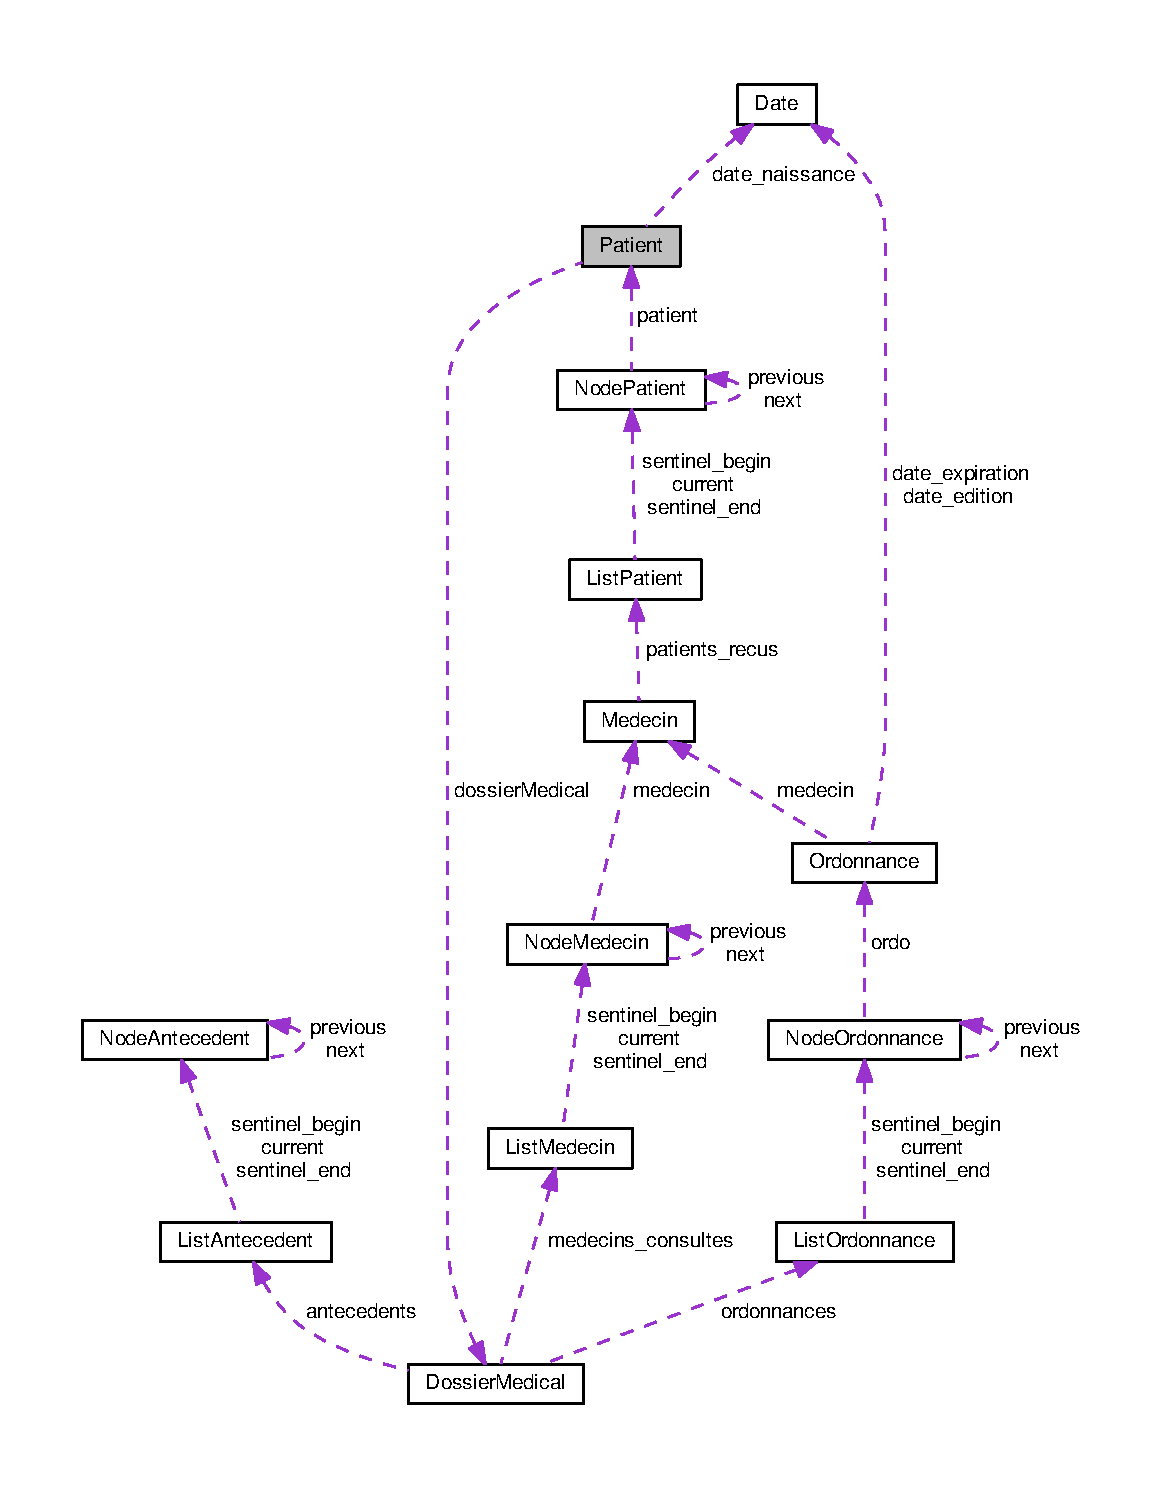
\includegraphics[width=350pt]{struct_patient__coll__graph}
\end{center}
\end{figure}
\subsection*{Champs de données}
\begin{DoxyCompactItemize}
\item 
char $\ast$ \hyperlink{struct_patient_abe308d273ff51ad86ff02ef3ba3b6f0e}{nom}
\item 
char $\ast$ \hyperlink{struct_patient_aa7d0e9e8505d2ac627777c4168573ec9}{prenom}
\item 
\hyperlink{struct_date}{Date} $\ast$ \hyperlink{struct_patient_a1ce5c592705142193b097a1bed2794e6}{date\-\_\-naissance}
\item 
char $\ast$ \hyperlink{struct_patient_aefa944e4b78fb9e14c4f6e49605bba2c}{adresse\-\_\-mail}
\item 
char $\ast$ \hyperlink{struct_patient_ac65f93b2b15c34c800c05832e346c98f}{numero\-\_\-telephone}
\item 
char $\ast$ \hyperlink{struct_patient_a49bbab73f86aafe9ee3ef4b862946698}{numero\-\_\-secu\-\_\-social}
\item 
\hyperlink{struct_dossier_medical}{Dossier\-Medical} $\ast$ \hyperlink{struct_patient_a7b81f4ba7de896fa37673d677977cedf}{dossier\-Medical}
\end{DoxyCompactItemize}


\subsection{Description détaillée}
Structure patient représentant un patient qui vient consulté dans l'application 

\subsection{Documentation des champs}
\hypertarget{struct_patient_aefa944e4b78fb9e14c4f6e49605bba2c}{\index{Patient@{Patient}!adresse\-\_\-mail@{adresse\-\_\-mail}}
\index{adresse\-\_\-mail@{adresse\-\_\-mail}!Patient@{Patient}}
\subsubsection[{adresse\-\_\-mail}]{\setlength{\rightskip}{0pt plus 5cm}char$\ast$ adresse\-\_\-mail}}\label{struct_patient_aefa944e4b78fb9e14c4f6e49605bba2c}
\hypertarget{struct_patient_a1ce5c592705142193b097a1bed2794e6}{\index{Patient@{Patient}!date\-\_\-naissance@{date\-\_\-naissance}}
\index{date\-\_\-naissance@{date\-\_\-naissance}!Patient@{Patient}}
\subsubsection[{date\-\_\-naissance}]{\setlength{\rightskip}{0pt plus 5cm}{\bf Date}$\ast$ date\-\_\-naissance}}\label{struct_patient_a1ce5c592705142193b097a1bed2794e6}
\hypertarget{struct_patient_a7b81f4ba7de896fa37673d677977cedf}{\index{Patient@{Patient}!dossier\-Medical@{dossier\-Medical}}
\index{dossier\-Medical@{dossier\-Medical}!Patient@{Patient}}
\subsubsection[{dossier\-Medical}]{\setlength{\rightskip}{0pt plus 5cm}{\bf Dossier\-Medical}$\ast$ dossier\-Medical}}\label{struct_patient_a7b81f4ba7de896fa37673d677977cedf}
\hypertarget{struct_patient_abe308d273ff51ad86ff02ef3ba3b6f0e}{\index{Patient@{Patient}!nom@{nom}}
\index{nom@{nom}!Patient@{Patient}}
\subsubsection[{nom}]{\setlength{\rightskip}{0pt plus 5cm}char$\ast$ nom}}\label{struct_patient_abe308d273ff51ad86ff02ef3ba3b6f0e}
\hypertarget{struct_patient_a49bbab73f86aafe9ee3ef4b862946698}{\index{Patient@{Patient}!numero\-\_\-secu\-\_\-social@{numero\-\_\-secu\-\_\-social}}
\index{numero\-\_\-secu\-\_\-social@{numero\-\_\-secu\-\_\-social}!Patient@{Patient}}
\subsubsection[{numero\-\_\-secu\-\_\-social}]{\setlength{\rightskip}{0pt plus 5cm}char$\ast$ numero\-\_\-secu\-\_\-social}}\label{struct_patient_a49bbab73f86aafe9ee3ef4b862946698}
\hypertarget{struct_patient_ac65f93b2b15c34c800c05832e346c98f}{\index{Patient@{Patient}!numero\-\_\-telephone@{numero\-\_\-telephone}}
\index{numero\-\_\-telephone@{numero\-\_\-telephone}!Patient@{Patient}}
\subsubsection[{numero\-\_\-telephone}]{\setlength{\rightskip}{0pt plus 5cm}char$\ast$ numero\-\_\-telephone}}\label{struct_patient_ac65f93b2b15c34c800c05832e346c98f}
\hypertarget{struct_patient_aa7d0e9e8505d2ac627777c4168573ec9}{\index{Patient@{Patient}!prenom@{prenom}}
\index{prenom@{prenom}!Patient@{Patient}}
\subsubsection[{prenom}]{\setlength{\rightskip}{0pt plus 5cm}char$\ast$ prenom}}\label{struct_patient_aa7d0e9e8505d2ac627777c4168573ec9}


La documentation de cette structure a été générée à partir du fichier suivant \-:\begin{DoxyCompactItemize}
\item 
include/\-G\-P\-Calendar/\-Model/\hyperlink{patient_8h}{patient.\-h}\end{DoxyCompactItemize}

\hypertarget{struct_project}{\section{Référence de la structure Project}
\label{struct_project}\index{Project@{Project}}
}


{\ttfamily \#include $<$Json\-Save.\-h$>$}



Graphe de collaboration de Project\-:
\nopagebreak
\begin{figure}[H]
\begin{center}
\leavevmode
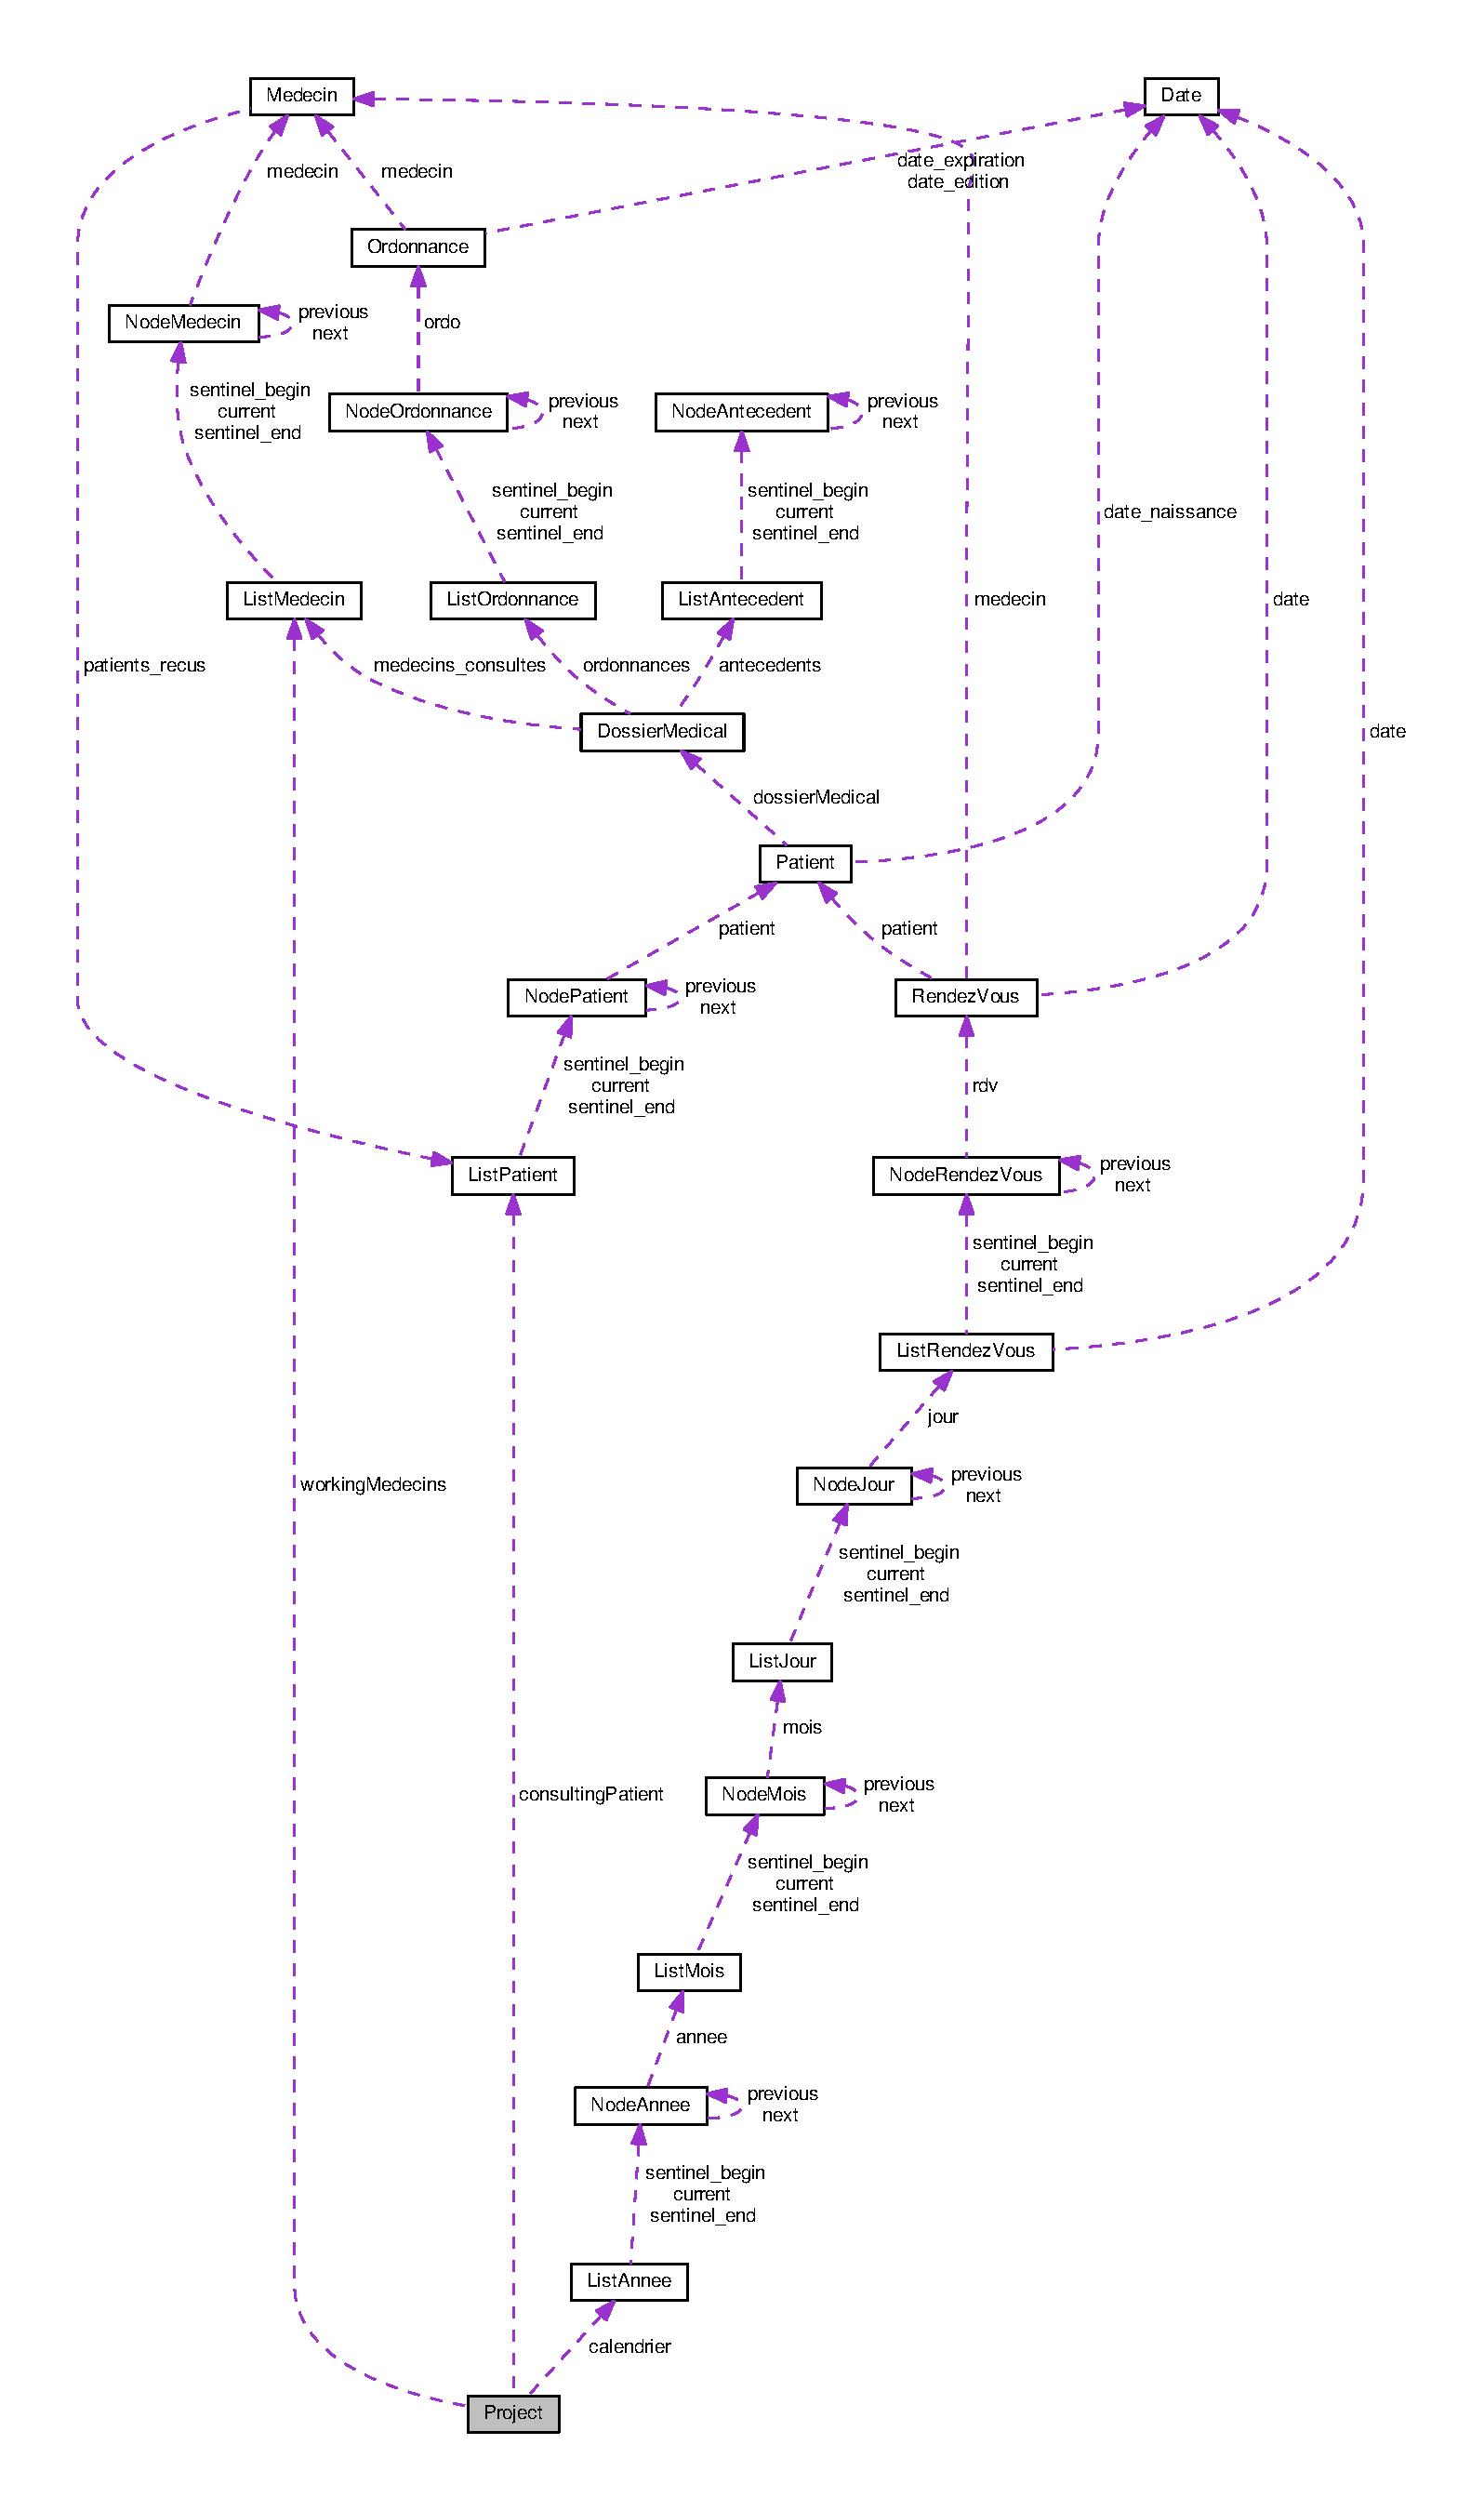
\includegraphics[height=550pt]{struct_project__coll__graph}
\end{center}
\end{figure}
\subsection*{Champs de données}
\begin{DoxyCompactItemize}
\item 
char $\ast$ \hyperlink{struct_project_abe308d273ff51ad86ff02ef3ba3b6f0e}{nom}
\item 
\hyperlink{struct_list_medecin}{List\-Medecin} $\ast$ \hyperlink{struct_project_ad698f4218c3645e84ec3b943db9ea06d}{working\-Medecins}
\item 
\hyperlink{struct_list_patient}{List\-Patient} $\ast$ \hyperlink{struct_project_a5a3570c43d186ae075a0d893438ce8b4}{consulting\-Patient}
\item 
\hyperlink{calendrier_8h_ab8644d1026df84be3eb3190cf1ef29fa}{Calendrier} \hyperlink{struct_project_ac1c68d1c7eeee118cba12c3efab5fd3f}{calendrier}
\end{DoxyCompactItemize}


\subsection{Documentation des champs}
\hypertarget{struct_project_ac1c68d1c7eeee118cba12c3efab5fd3f}{\index{Project@{Project}!calendrier@{calendrier}}
\index{calendrier@{calendrier}!Project@{Project}}
\subsubsection[{calendrier}]{\setlength{\rightskip}{0pt plus 5cm}{\bf Calendrier} calendrier}}\label{struct_project_ac1c68d1c7eeee118cba12c3efab5fd3f}
\hypertarget{struct_project_a5a3570c43d186ae075a0d893438ce8b4}{\index{Project@{Project}!consulting\-Patient@{consulting\-Patient}}
\index{consulting\-Patient@{consulting\-Patient}!Project@{Project}}
\subsubsection[{consulting\-Patient}]{\setlength{\rightskip}{0pt plus 5cm}{\bf List\-Patient}$\ast$ consulting\-Patient}}\label{struct_project_a5a3570c43d186ae075a0d893438ce8b4}
\hypertarget{struct_project_abe308d273ff51ad86ff02ef3ba3b6f0e}{\index{Project@{Project}!nom@{nom}}
\index{nom@{nom}!Project@{Project}}
\subsubsection[{nom}]{\setlength{\rightskip}{0pt plus 5cm}char$\ast$ nom}}\label{struct_project_abe308d273ff51ad86ff02ef3ba3b6f0e}
\hypertarget{struct_project_ad698f4218c3645e84ec3b943db9ea06d}{\index{Project@{Project}!working\-Medecins@{working\-Medecins}}
\index{working\-Medecins@{working\-Medecins}!Project@{Project}}
\subsubsection[{working\-Medecins}]{\setlength{\rightskip}{0pt plus 5cm}{\bf List\-Medecin}$\ast$ working\-Medecins}}\label{struct_project_ad698f4218c3645e84ec3b943db9ea06d}


La documentation de cette structure a été générée à partir du fichier suivant \-:\begin{DoxyCompactItemize}
\item 
include/\-G\-P\-Calendar/\-Model/\hyperlink{_json_save_8h}{Json\-Save.\-h}\end{DoxyCompactItemize}

\hypertarget{struct_rendez_vous}{\section{Référence de la structure Rendez\-Vous}
\label{struct_rendez_vous}\index{Rendez\-Vous@{Rendez\-Vous}}
}


{\ttfamily \#include $<$rendezvous.\-h$>$}



Graphe de collaboration de Rendez\-Vous\-:
\nopagebreak
\begin{figure}[H]
\begin{center}
\leavevmode
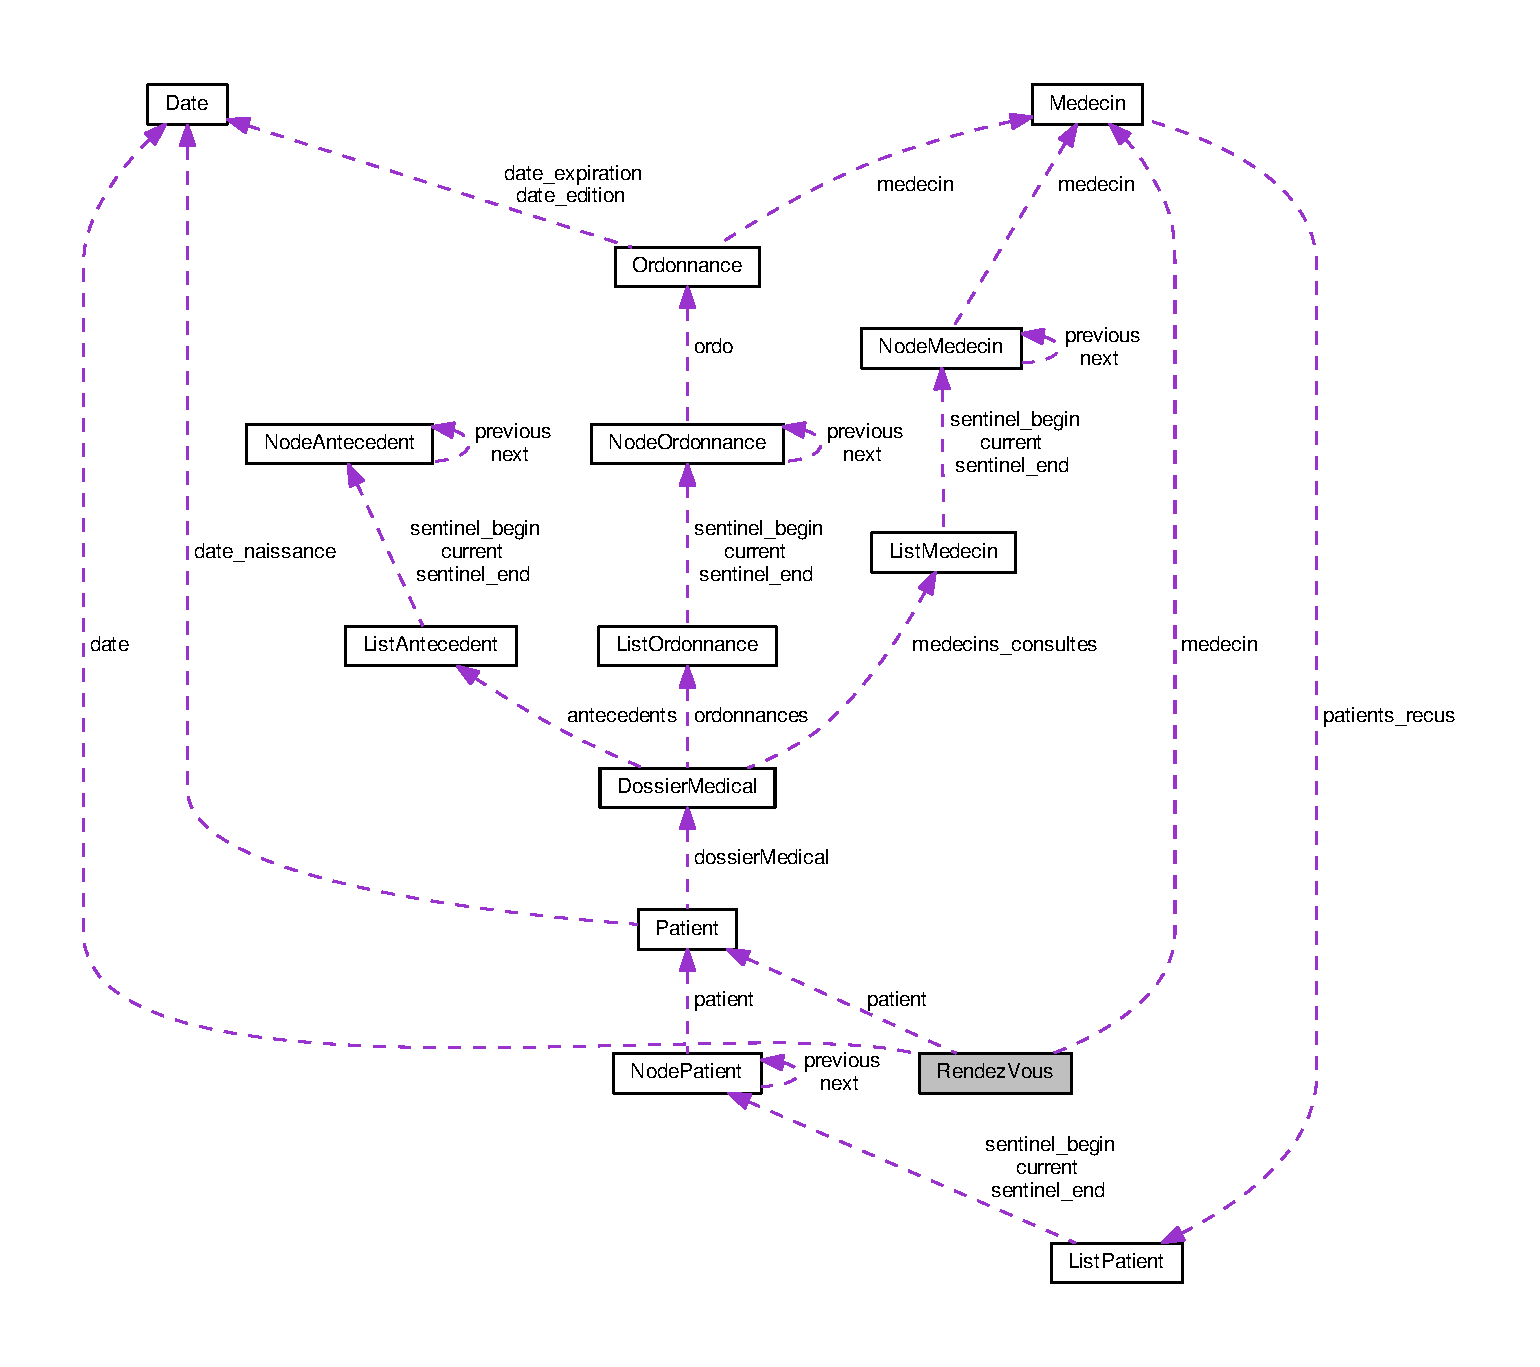
\includegraphics[width=350pt]{struct_rendez_vous__coll__graph}
\end{center}
\end{figure}
\subsection*{Champs de données}
\begin{DoxyCompactItemize}
\item 
\hyperlink{struct_date}{Date} $\ast$ \hyperlink{struct_rendez_vous_a73fc78564c9badbcea68f2f2331c74db}{date}
\item 
double \hyperlink{struct_rendez_vous_a3877de0db2ba94f6179438f6ce2d79e4}{heure\-\_\-debut}
\item 
double \hyperlink{struct_rendez_vous_a91f724ef59fa01719e26c722ce70666f}{heure\-\_\-fin}
\item 
char $\ast$ \hyperlink{struct_rendez_vous_a4e5bf777d1128fd5e62442afa61ea3c9}{lieu}
\item 
\hyperlink{struct_patient}{Patient} $\ast$ \hyperlink{struct_rendez_vous_a602d93e6dfbb9a54fc31419f2463ac2b}{patient}
\item 
\hyperlink{struct_medecin}{Medecin} $\ast$ \hyperlink{struct_rendez_vous_a59131973441fcf6250df021bcf96d17c}{medecin}
\item 
char $\ast$ \hyperlink{struct_rendez_vous_ac1d72cddca5f2d79a6b2691aacd03850}{motif}
\end{DoxyCompactItemize}


\subsection{Description détaillée}
Ou est-\/ce qu'on free nos objets Rendez-\/\-Vous ? Vrai question \-: ds le calendrier ou lorsqu'on ferme l'appli ? Demander au prof 

\subsection{Documentation des champs}
\hypertarget{struct_rendez_vous_a73fc78564c9badbcea68f2f2331c74db}{\index{Rendez\-Vous@{Rendez\-Vous}!date@{date}}
\index{date@{date}!RendezVous@{Rendez\-Vous}}
\subsubsection[{date}]{\setlength{\rightskip}{0pt plus 5cm}{\bf Date}$\ast$ date}}\label{struct_rendez_vous_a73fc78564c9badbcea68f2f2331c74db}
\hypertarget{struct_rendez_vous_a3877de0db2ba94f6179438f6ce2d79e4}{\index{Rendez\-Vous@{Rendez\-Vous}!heure\-\_\-debut@{heure\-\_\-debut}}
\index{heure\-\_\-debut@{heure\-\_\-debut}!RendezVous@{Rendez\-Vous}}
\subsubsection[{heure\-\_\-debut}]{\setlength{\rightskip}{0pt plus 5cm}double heure\-\_\-debut}}\label{struct_rendez_vous_a3877de0db2ba94f6179438f6ce2d79e4}
\hypertarget{struct_rendez_vous_a91f724ef59fa01719e26c722ce70666f}{\index{Rendez\-Vous@{Rendez\-Vous}!heure\-\_\-fin@{heure\-\_\-fin}}
\index{heure\-\_\-fin@{heure\-\_\-fin}!RendezVous@{Rendez\-Vous}}
\subsubsection[{heure\-\_\-fin}]{\setlength{\rightskip}{0pt plus 5cm}double heure\-\_\-fin}}\label{struct_rendez_vous_a91f724ef59fa01719e26c722ce70666f}
\hypertarget{struct_rendez_vous_a4e5bf777d1128fd5e62442afa61ea3c9}{\index{Rendez\-Vous@{Rendez\-Vous}!lieu@{lieu}}
\index{lieu@{lieu}!RendezVous@{Rendez\-Vous}}
\subsubsection[{lieu}]{\setlength{\rightskip}{0pt plus 5cm}char$\ast$ lieu}}\label{struct_rendez_vous_a4e5bf777d1128fd5e62442afa61ea3c9}
\hypertarget{struct_rendez_vous_a59131973441fcf6250df021bcf96d17c}{\index{Rendez\-Vous@{Rendez\-Vous}!medecin@{medecin}}
\index{medecin@{medecin}!RendezVous@{Rendez\-Vous}}
\subsubsection[{medecin}]{\setlength{\rightskip}{0pt plus 5cm}{\bf Medecin}$\ast$ medecin}}\label{struct_rendez_vous_a59131973441fcf6250df021bcf96d17c}
\hypertarget{struct_rendez_vous_ac1d72cddca5f2d79a6b2691aacd03850}{\index{Rendez\-Vous@{Rendez\-Vous}!motif@{motif}}
\index{motif@{motif}!RendezVous@{Rendez\-Vous}}
\subsubsection[{motif}]{\setlength{\rightskip}{0pt plus 5cm}char$\ast$ motif}}\label{struct_rendez_vous_ac1d72cddca5f2d79a6b2691aacd03850}
\hypertarget{struct_rendez_vous_a602d93e6dfbb9a54fc31419f2463ac2b}{\index{Rendez\-Vous@{Rendez\-Vous}!patient@{patient}}
\index{patient@{patient}!RendezVous@{Rendez\-Vous}}
\subsubsection[{patient}]{\setlength{\rightskip}{0pt plus 5cm}{\bf Patient}$\ast$ patient}}\label{struct_rendez_vous_a602d93e6dfbb9a54fc31419f2463ac2b}


La documentation de cette structure a été générée à partir du fichier suivant \-:\begin{DoxyCompactItemize}
\item 
include/\-G\-P\-Calendar/\-Model/\hyperlink{rendezvous_8h}{rendezvous.\-h}\end{DoxyCompactItemize}

\chapter{Documentation des fichiers}
\hypertarget{_g_p_calendar_shell_8h}{\section{Référence du fichier include/\-G\-P\-Calendar/\-App/\-G\-P\-Calendar\-Shell.h}
\label{_g_p_calendar_shell_8h}\index{include/\-G\-P\-Calendar/\-App/\-G\-P\-Calendar\-Shell.\-h@{include/\-G\-P\-Calendar/\-App/\-G\-P\-Calendar\-Shell.\-h}}
}
{\ttfamily \#include \char`\"{}G\-P\-Calendar/\-Model/\-Json\-Save.\-h\char`\"{}}\\*
{\ttfamily \#include \char`\"{}G\-P\-Calendar/\-Model/medecin.\-h\char`\"{}}\\*
{\ttfamily \#include \char`\"{}G\-P\-Calendar/\-Model/patient.\-h\char`\"{}}\\*
{\ttfamily \#include \char`\"{}G\-P\-Calendar/\-Model/date.\-h\char`\"{}}\\*
{\ttfamily \#include \char`\"{}G\-P\-Calendar/\-Model/calendrier.\-h\char`\"{}}\\*
{\ttfamily \#include \char`\"{}G\-P\-Calendar/\-Model/ordonnance.\-h\char`\"{}}\\*
{\ttfamily \#include \char`\"{}G\-P\-Calendar/\-Model/dossier\-\_\-medical.\-h\char`\"{}}\\*
{\ttfamily \#include \char`\"{}G\-P\-Calendar/\-Model/rendezvous.\-h\char`\"{}}\\*
{\ttfamily \#include $<$stdlib.\-h$>$}\\*
{\ttfamily \#include $<$stdio.\-h$>$}\\*
{\ttfamily \#include $<$string.\-h$>$}\\*
Graphe des dépendances par inclusion de G\-P\-Calendar\-Shell.\-h\-:
\nopagebreak
\begin{figure}[H]
\begin{center}
\leavevmode
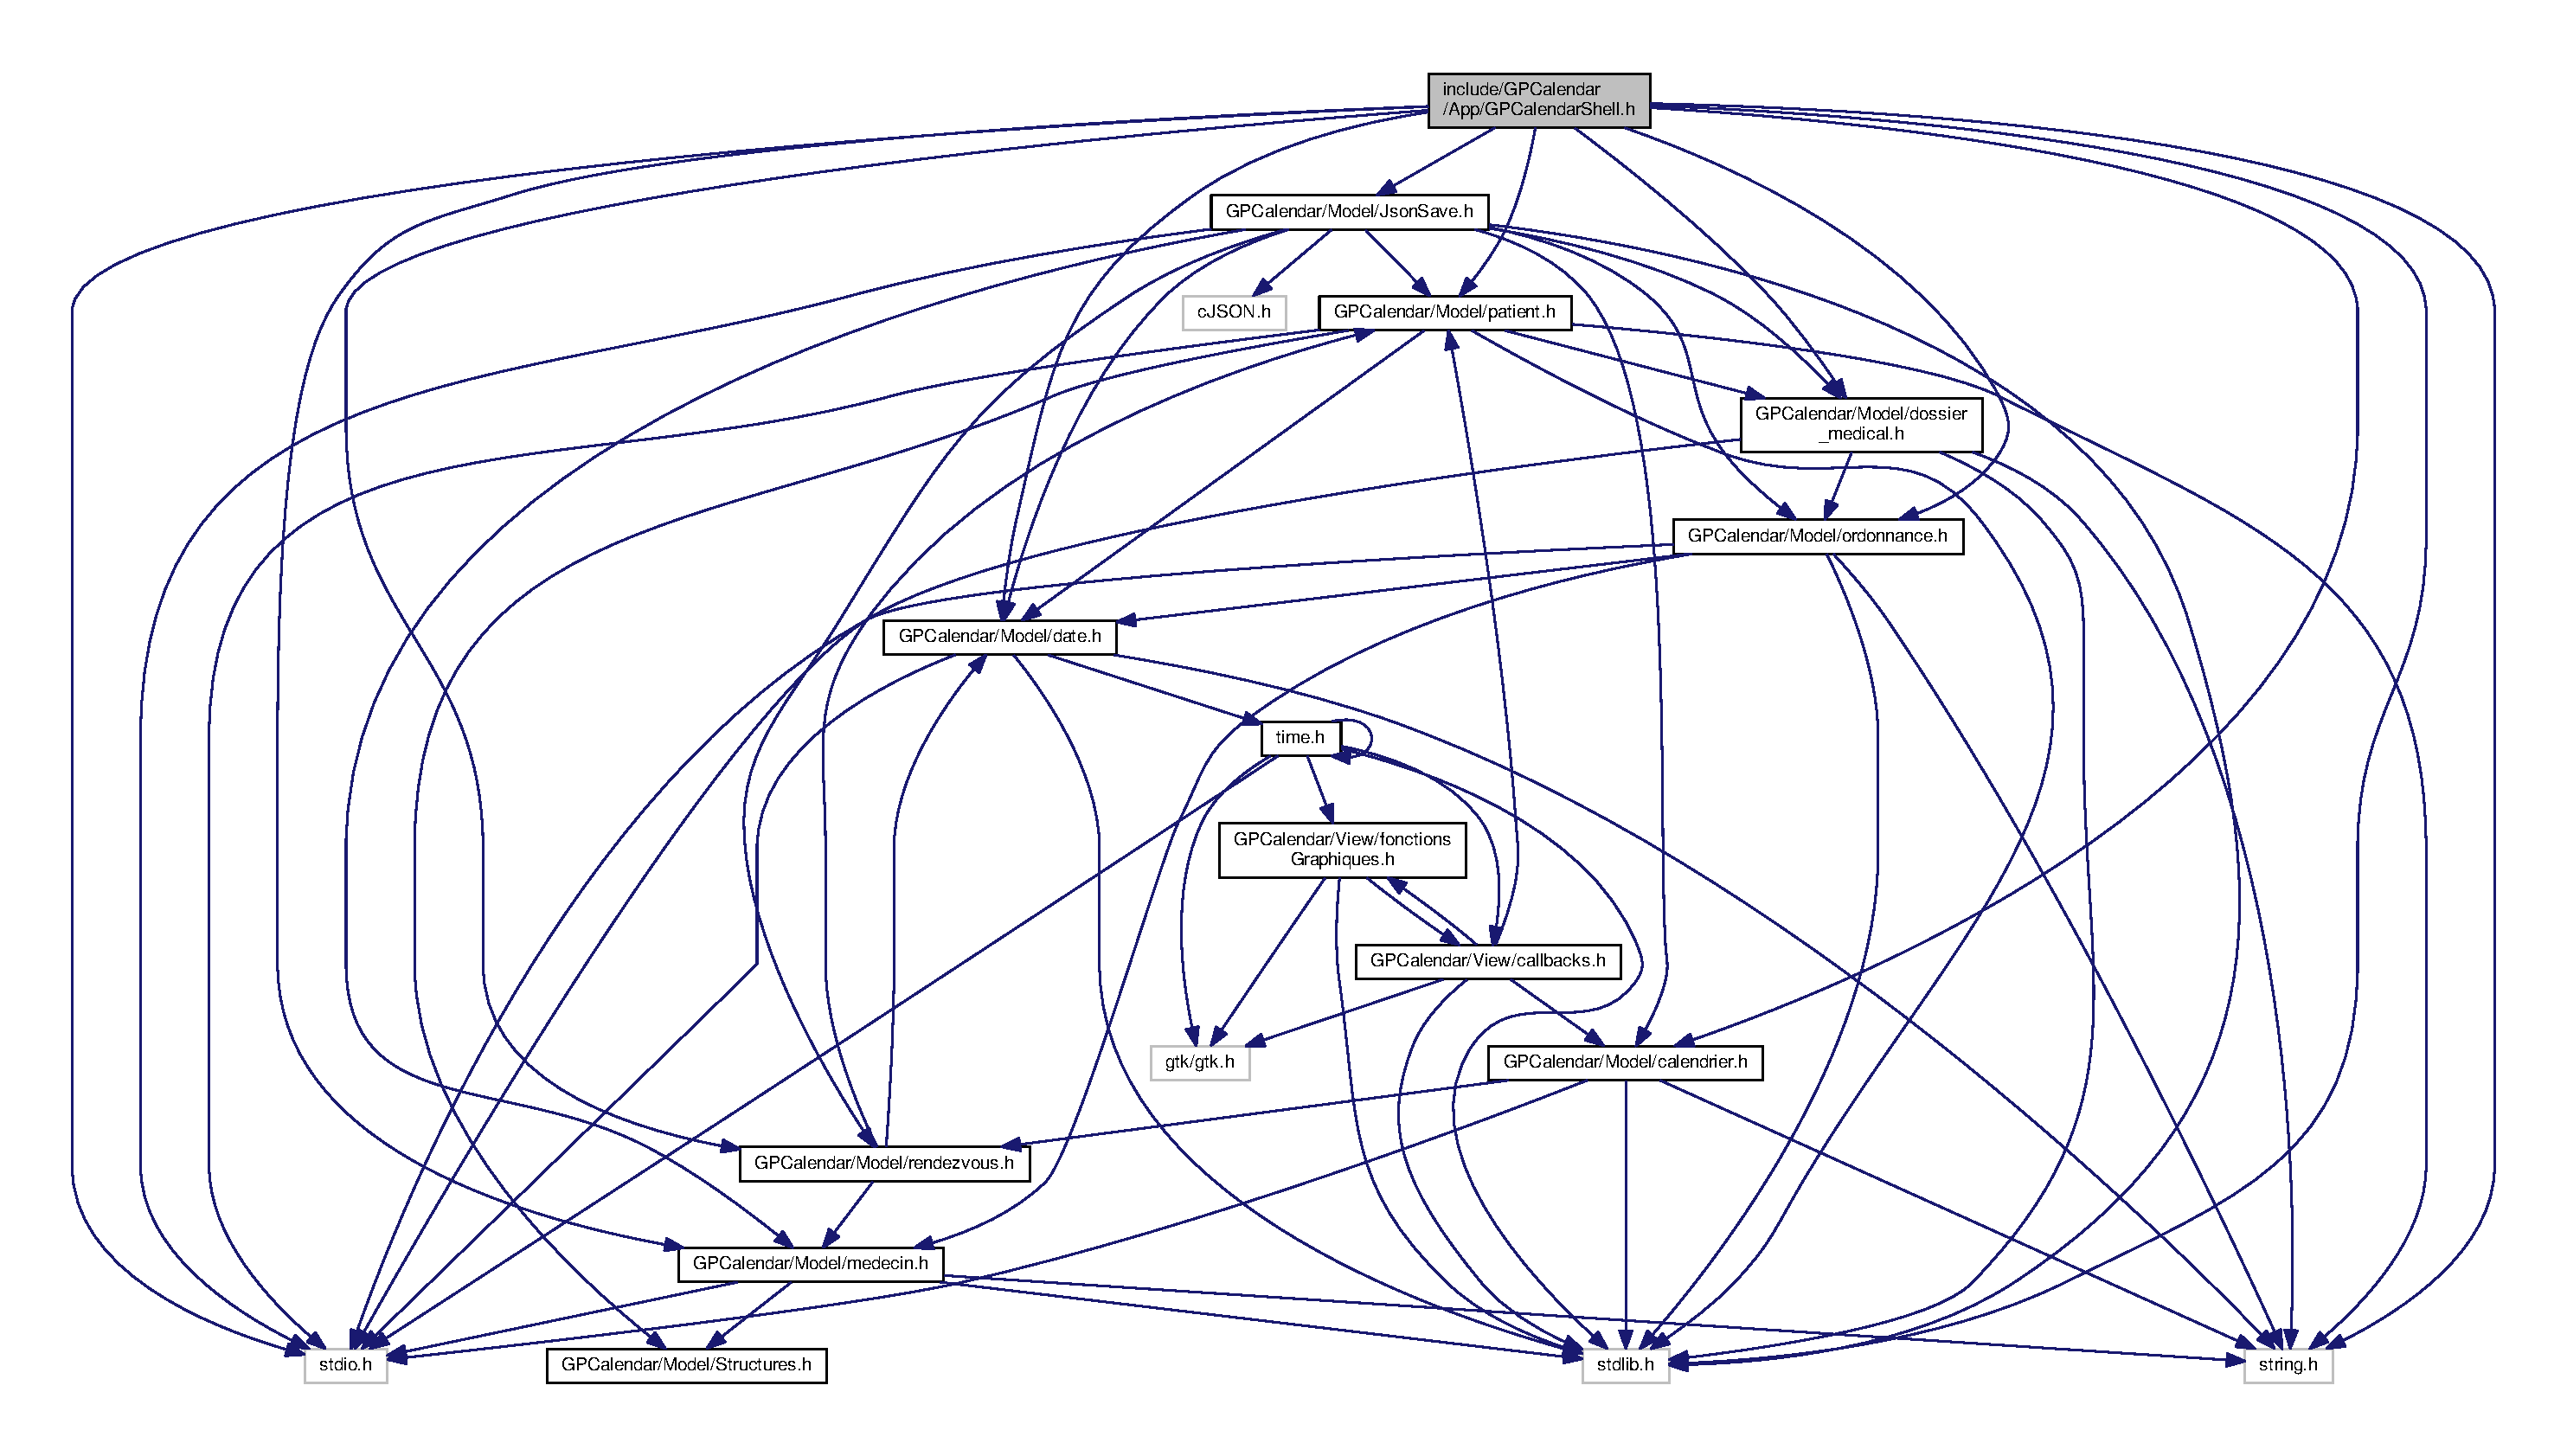
\includegraphics[width=350pt]{_g_p_calendar_shell_8h__incl}
\end{center}
\end{figure}
Ce graphe montre quels fichiers incluent directement ou indirectement ce fichier \-:
\nopagebreak
\begin{figure}[H]
\begin{center}
\leavevmode
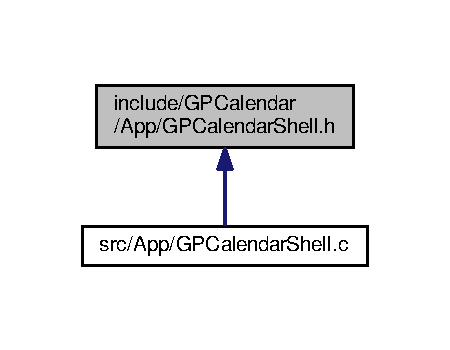
\includegraphics[width=216pt]{_g_p_calendar_shell_8h__dep__incl}
\end{center}
\end{figure}
\subsection*{Fonctions}
\begin{DoxyCompactItemize}
\item 
void \hyperlink{_g_p_calendar_shell_8h_aeb5ca1f06d1f2130fd3df595b9099d3e}{print\-Possible\-Action} ()
\item 
void \hyperlink{_g_p_calendar_shell_8h_adc1f84aaf9010381b234f55a21f7ee27}{Shell\-\_\-creer\-Patient} ()
\item 
void \hyperlink{_g_p_calendar_shell_8h_a4c4a1b40f22e7ba418d1cdd9d112c6a0}{Shell\-\_\-creer\-Medecin} ()
\item 
void \hyperlink{_g_p_calendar_shell_8h_a51b83637c6c6d85cdf3cbf3293de4c5e}{Shell\-\_\-creer\-Rendez\-Vous} ()
\item 
void \hyperlink{_g_p_calendar_shell_8h_adde2df8834cf928dc1575bdd79a319a1}{Shell\-\_\-consulter\-Informations} ()
\item 
void \hyperlink{_g_p_calendar_shell_8h_a9998da37fd86e0715bc3c32a8b03aa75}{Shell\-\_\-annuler\-Rendez\-Vous} ()
\item 
void \hyperlink{_g_p_calendar_shell_8h_a4b5636f1ce8664a9fd3f013974f5e38b}{Shell\-\_\-supprimer\-Patient} ()
\item 
void \hyperlink{_g_p_calendar_shell_8h_adb25a8730eec229efe99eaa5515973fc}{Shell\-\_\-supprimer\-Medecin} ()
\item 
void \hyperlink{_g_p_calendar_shell_8h_af30486979761ada08a0cb4829c382b88}{Shell\-\_\-save\-Project} ()
\item 
void \hyperlink{_g_p_calendar_shell_8h_a5a9b0cab040661b28215cc7d24108141}{Shell\-\_\-load\-Project} ()
\end{DoxyCompactItemize}


\subsection{Documentation des fonctions}
\hypertarget{_g_p_calendar_shell_8h_aeb5ca1f06d1f2130fd3df595b9099d3e}{\index{G\-P\-Calendar\-Shell.\-h@{G\-P\-Calendar\-Shell.\-h}!print\-Possible\-Action@{print\-Possible\-Action}}
\index{print\-Possible\-Action@{print\-Possible\-Action}!GPCalendarShell.h@{G\-P\-Calendar\-Shell.\-h}}
\subsubsection[{print\-Possible\-Action}]{\setlength{\rightskip}{0pt plus 5cm}void print\-Possible\-Action (
\begin{DoxyParamCaption}
{}
\end{DoxyParamCaption}
)}}\label{_g_p_calendar_shell_8h_aeb5ca1f06d1f2130fd3df595b9099d3e}
\hypertarget{_g_p_calendar_shell_8h_a9998da37fd86e0715bc3c32a8b03aa75}{\index{G\-P\-Calendar\-Shell.\-h@{G\-P\-Calendar\-Shell.\-h}!Shell\-\_\-annuler\-Rendez\-Vous@{Shell\-\_\-annuler\-Rendez\-Vous}}
\index{Shell\-\_\-annuler\-Rendez\-Vous@{Shell\-\_\-annuler\-Rendez\-Vous}!GPCalendarShell.h@{G\-P\-Calendar\-Shell.\-h}}
\subsubsection[{Shell\-\_\-annuler\-Rendez\-Vous}]{\setlength{\rightskip}{0pt plus 5cm}void Shell\-\_\-annuler\-Rendez\-Vous (
\begin{DoxyParamCaption}
{}
\end{DoxyParamCaption}
)}}\label{_g_p_calendar_shell_8h_a9998da37fd86e0715bc3c32a8b03aa75}
\hypertarget{_g_p_calendar_shell_8h_adde2df8834cf928dc1575bdd79a319a1}{\index{G\-P\-Calendar\-Shell.\-h@{G\-P\-Calendar\-Shell.\-h}!Shell\-\_\-consulter\-Informations@{Shell\-\_\-consulter\-Informations}}
\index{Shell\-\_\-consulter\-Informations@{Shell\-\_\-consulter\-Informations}!GPCalendarShell.h@{G\-P\-Calendar\-Shell.\-h}}
\subsubsection[{Shell\-\_\-consulter\-Informations}]{\setlength{\rightskip}{0pt plus 5cm}void Shell\-\_\-consulter\-Informations (
\begin{DoxyParamCaption}
{}
\end{DoxyParamCaption}
)}}\label{_g_p_calendar_shell_8h_adde2df8834cf928dc1575bdd79a319a1}
\hypertarget{_g_p_calendar_shell_8h_a4c4a1b40f22e7ba418d1cdd9d112c6a0}{\index{G\-P\-Calendar\-Shell.\-h@{G\-P\-Calendar\-Shell.\-h}!Shell\-\_\-creer\-Medecin@{Shell\-\_\-creer\-Medecin}}
\index{Shell\-\_\-creer\-Medecin@{Shell\-\_\-creer\-Medecin}!GPCalendarShell.h@{G\-P\-Calendar\-Shell.\-h}}
\subsubsection[{Shell\-\_\-creer\-Medecin}]{\setlength{\rightskip}{0pt plus 5cm}void Shell\-\_\-creer\-Medecin (
\begin{DoxyParamCaption}
{}
\end{DoxyParamCaption}
)}}\label{_g_p_calendar_shell_8h_a4c4a1b40f22e7ba418d1cdd9d112c6a0}
\hypertarget{_g_p_calendar_shell_8h_adc1f84aaf9010381b234f55a21f7ee27}{\index{G\-P\-Calendar\-Shell.\-h@{G\-P\-Calendar\-Shell.\-h}!Shell\-\_\-creer\-Patient@{Shell\-\_\-creer\-Patient}}
\index{Shell\-\_\-creer\-Patient@{Shell\-\_\-creer\-Patient}!GPCalendarShell.h@{G\-P\-Calendar\-Shell.\-h}}
\subsubsection[{Shell\-\_\-creer\-Patient}]{\setlength{\rightskip}{0pt plus 5cm}void Shell\-\_\-creer\-Patient (
\begin{DoxyParamCaption}
{}
\end{DoxyParamCaption}
)}}\label{_g_p_calendar_shell_8h_adc1f84aaf9010381b234f55a21f7ee27}
\hypertarget{_g_p_calendar_shell_8h_a51b83637c6c6d85cdf3cbf3293de4c5e}{\index{G\-P\-Calendar\-Shell.\-h@{G\-P\-Calendar\-Shell.\-h}!Shell\-\_\-creer\-Rendez\-Vous@{Shell\-\_\-creer\-Rendez\-Vous}}
\index{Shell\-\_\-creer\-Rendez\-Vous@{Shell\-\_\-creer\-Rendez\-Vous}!GPCalendarShell.h@{G\-P\-Calendar\-Shell.\-h}}
\subsubsection[{Shell\-\_\-creer\-Rendez\-Vous}]{\setlength{\rightskip}{0pt plus 5cm}void Shell\-\_\-creer\-Rendez\-Vous (
\begin{DoxyParamCaption}
{}
\end{DoxyParamCaption}
)}}\label{_g_p_calendar_shell_8h_a51b83637c6c6d85cdf3cbf3293de4c5e}
\hypertarget{_g_p_calendar_shell_8h_a5a9b0cab040661b28215cc7d24108141}{\index{G\-P\-Calendar\-Shell.\-h@{G\-P\-Calendar\-Shell.\-h}!Shell\-\_\-load\-Project@{Shell\-\_\-load\-Project}}
\index{Shell\-\_\-load\-Project@{Shell\-\_\-load\-Project}!GPCalendarShell.h@{G\-P\-Calendar\-Shell.\-h}}
\subsubsection[{Shell\-\_\-load\-Project}]{\setlength{\rightskip}{0pt plus 5cm}void Shell\-\_\-load\-Project (
\begin{DoxyParamCaption}
{}
\end{DoxyParamCaption}
)}}\label{_g_p_calendar_shell_8h_a5a9b0cab040661b28215cc7d24108141}
\hypertarget{_g_p_calendar_shell_8h_af30486979761ada08a0cb4829c382b88}{\index{G\-P\-Calendar\-Shell.\-h@{G\-P\-Calendar\-Shell.\-h}!Shell\-\_\-save\-Project@{Shell\-\_\-save\-Project}}
\index{Shell\-\_\-save\-Project@{Shell\-\_\-save\-Project}!GPCalendarShell.h@{G\-P\-Calendar\-Shell.\-h}}
\subsubsection[{Shell\-\_\-save\-Project}]{\setlength{\rightskip}{0pt plus 5cm}void Shell\-\_\-save\-Project (
\begin{DoxyParamCaption}
{}
\end{DoxyParamCaption}
)}}\label{_g_p_calendar_shell_8h_af30486979761ada08a0cb4829c382b88}
\hypertarget{_g_p_calendar_shell_8h_adb25a8730eec229efe99eaa5515973fc}{\index{G\-P\-Calendar\-Shell.\-h@{G\-P\-Calendar\-Shell.\-h}!Shell\-\_\-supprimer\-Medecin@{Shell\-\_\-supprimer\-Medecin}}
\index{Shell\-\_\-supprimer\-Medecin@{Shell\-\_\-supprimer\-Medecin}!GPCalendarShell.h@{G\-P\-Calendar\-Shell.\-h}}
\subsubsection[{Shell\-\_\-supprimer\-Medecin}]{\setlength{\rightskip}{0pt plus 5cm}void Shell\-\_\-supprimer\-Medecin (
\begin{DoxyParamCaption}
{}
\end{DoxyParamCaption}
)}}\label{_g_p_calendar_shell_8h_adb25a8730eec229efe99eaa5515973fc}
\hypertarget{_g_p_calendar_shell_8h_a4b5636f1ce8664a9fd3f013974f5e38b}{\index{G\-P\-Calendar\-Shell.\-h@{G\-P\-Calendar\-Shell.\-h}!Shell\-\_\-supprimer\-Patient@{Shell\-\_\-supprimer\-Patient}}
\index{Shell\-\_\-supprimer\-Patient@{Shell\-\_\-supprimer\-Patient}!GPCalendarShell.h@{G\-P\-Calendar\-Shell.\-h}}
\subsubsection[{Shell\-\_\-supprimer\-Patient}]{\setlength{\rightskip}{0pt plus 5cm}void Shell\-\_\-supprimer\-Patient (
\begin{DoxyParamCaption}
{}
\end{DoxyParamCaption}
)}}\label{_g_p_calendar_shell_8h_a4b5636f1ce8664a9fd3f013974f5e38b}

\hypertarget{calendrier_8h}{\section{Référence du fichier include/\-G\-P\-Calendar/\-Model/calendrier.h}
\label{calendrier_8h}\index{include/\-G\-P\-Calendar/\-Model/calendrier.\-h@{include/\-G\-P\-Calendar/\-Model/calendrier.\-h}}
}
{\ttfamily \#include \char`\"{}G\-P\-Calendar/\-Model/rendezvous.\-h\char`\"{}}\\*
{\ttfamily \#include $<$stdlib.\-h$>$}\\*
{\ttfamily \#include $<$stdio.\-h$>$}\\*
{\ttfamily \#include $<$string.\-h$>$}\\*
Graphe des dépendances par inclusion de calendrier.\-h\-:
\nopagebreak
\begin{figure}[H]
\begin{center}
\leavevmode
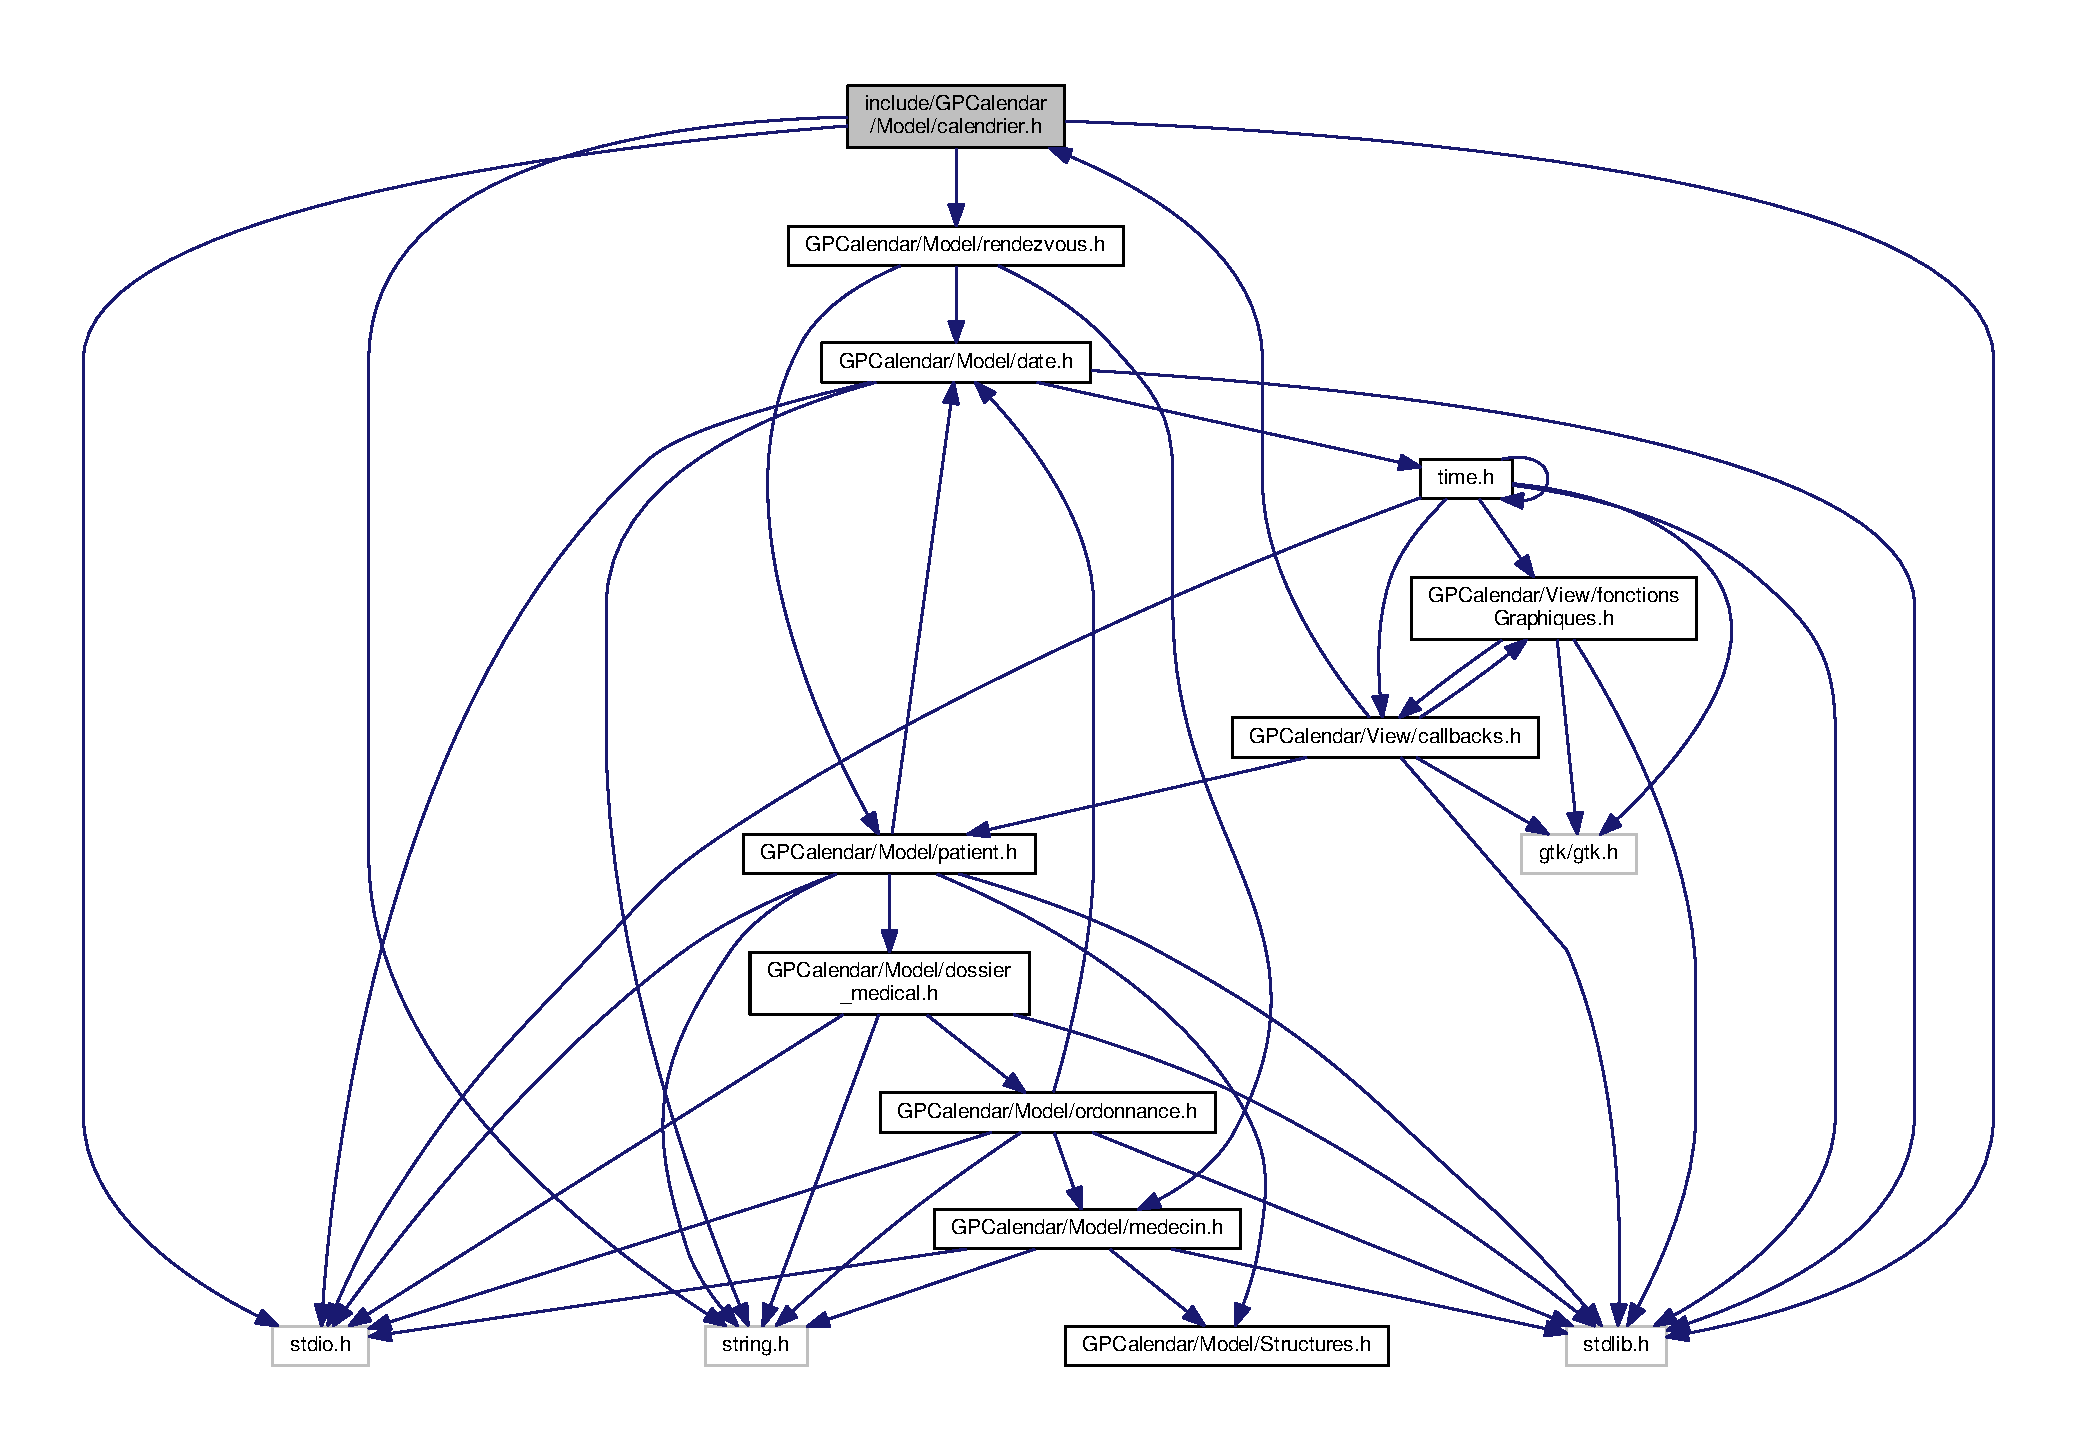
\includegraphics[width=350pt]{calendrier_8h__incl}
\end{center}
\end{figure}
Ce graphe montre quels fichiers incluent directement ou indirectement ce fichier \-:
\nopagebreak
\begin{figure}[H]
\begin{center}
\leavevmode
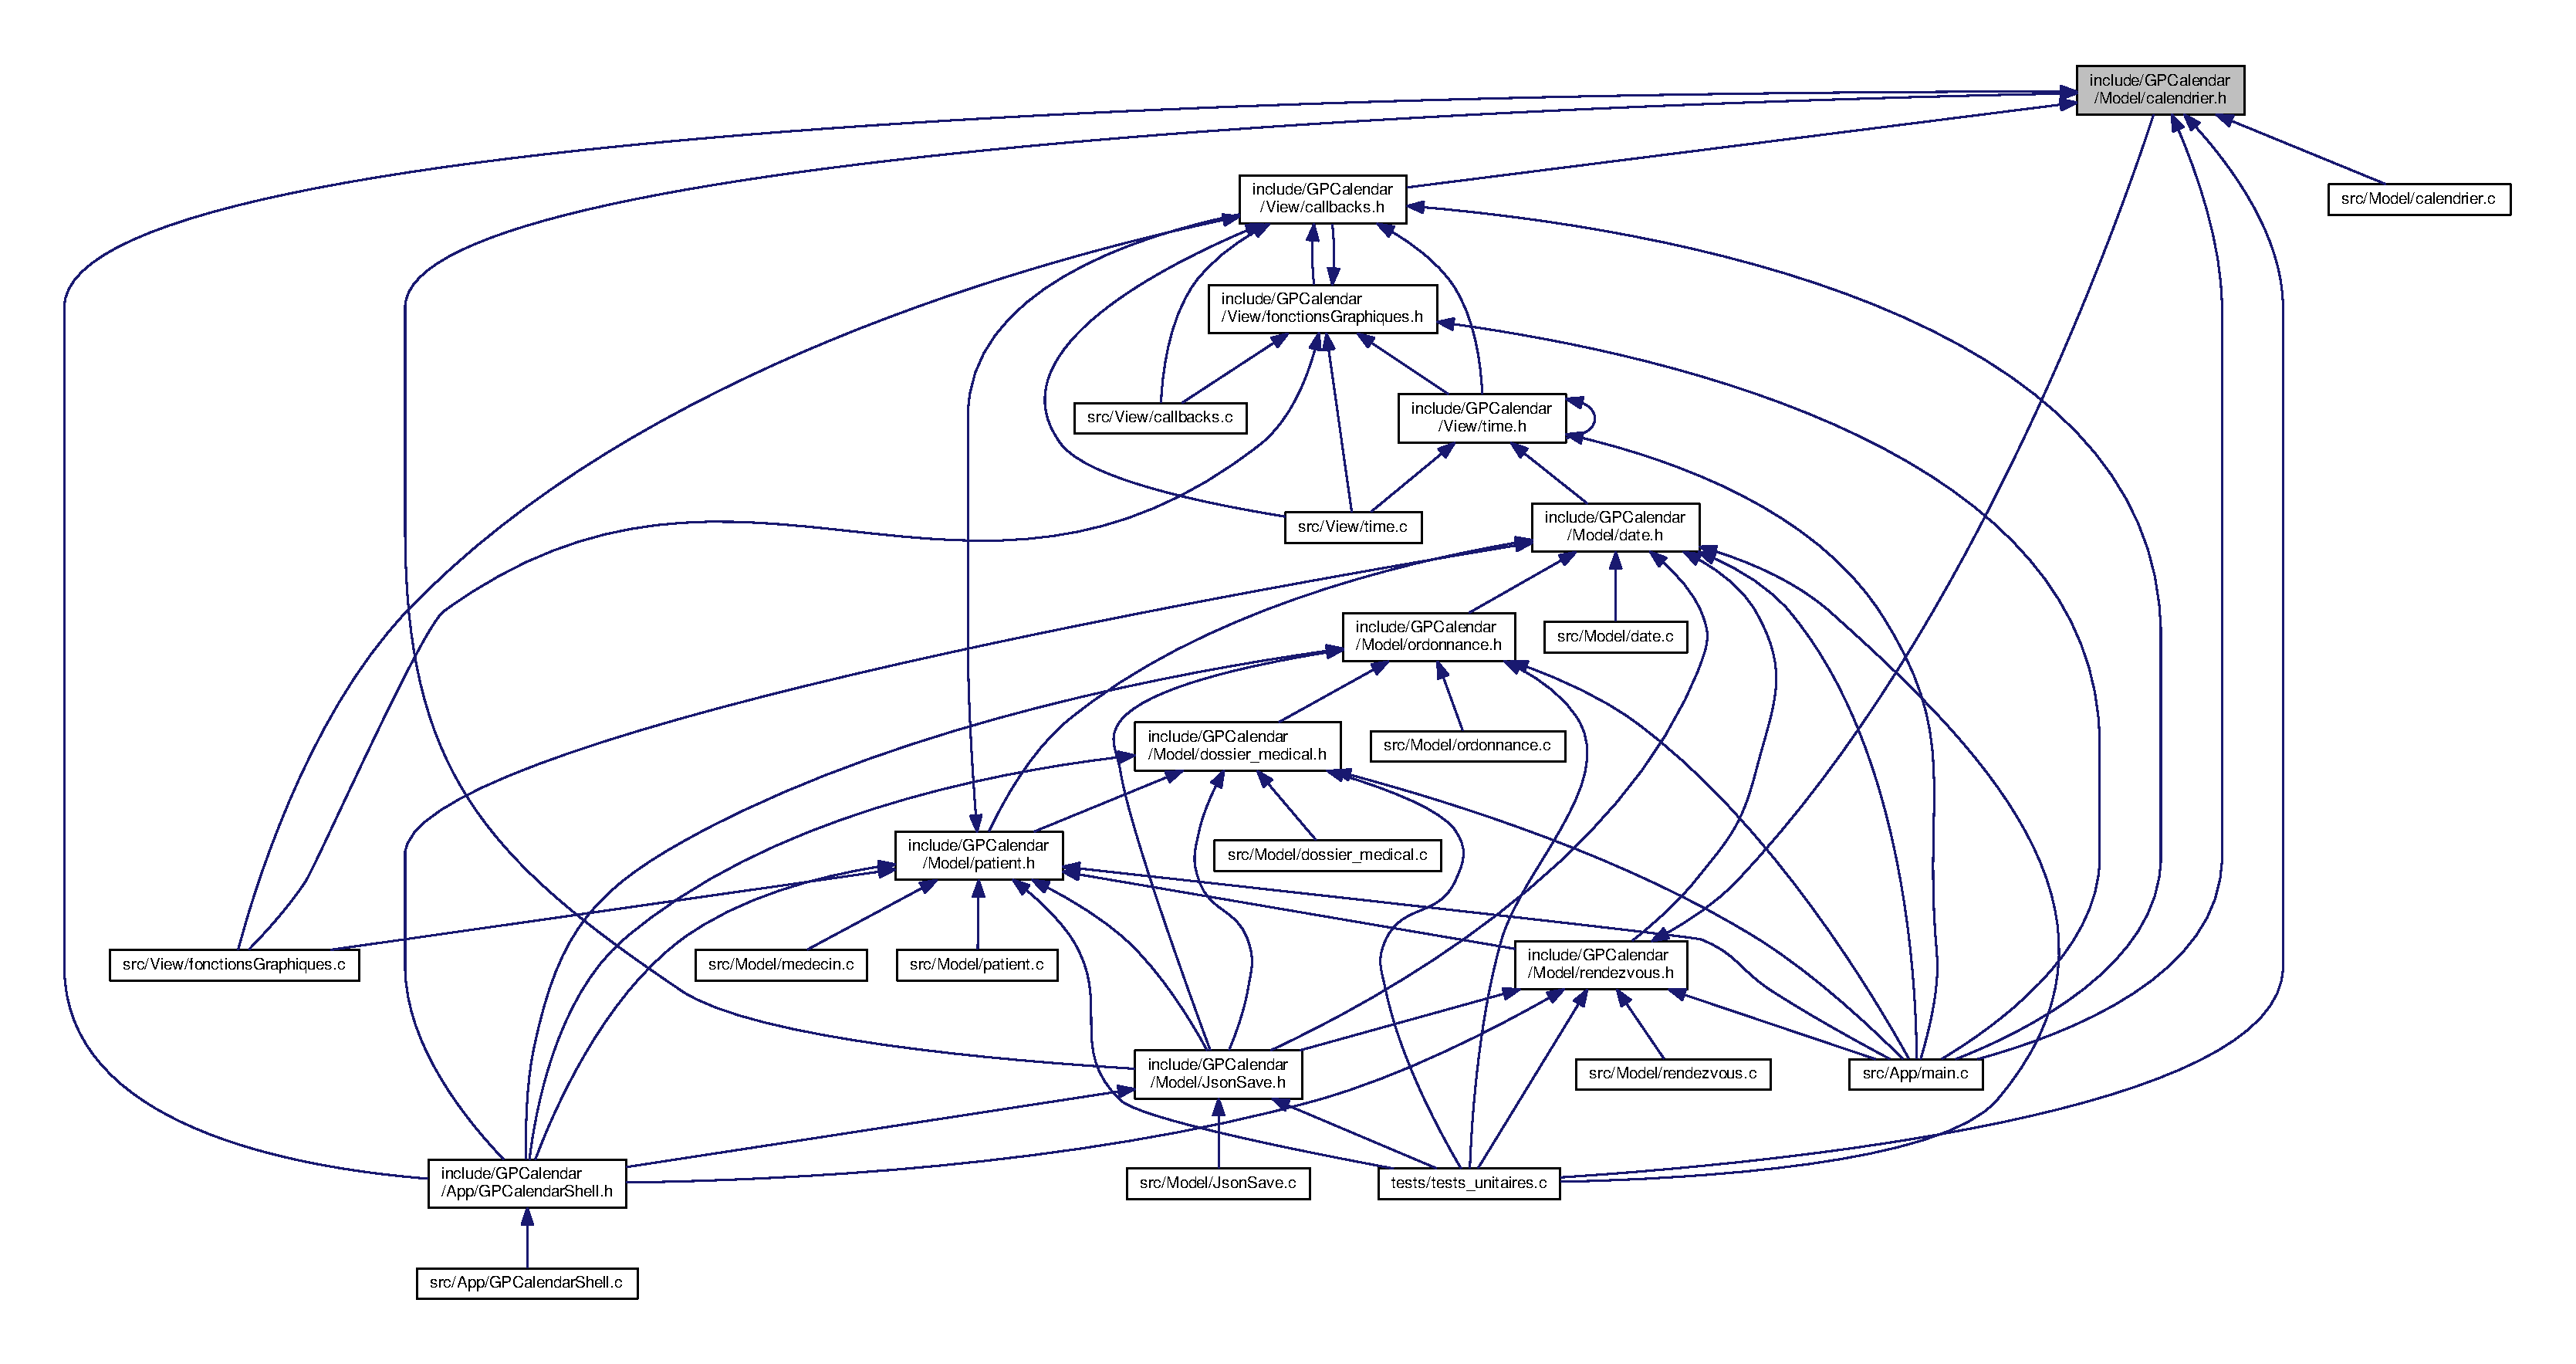
\includegraphics[width=350pt]{calendrier_8h__dep__incl}
\end{center}
\end{figure}
\subsection*{Structures de données}
\begin{DoxyCompactItemize}
\item 
struct \hyperlink{struct_node_rendez_vous}{Node\-Rendez\-Vous}
\item 
struct \hyperlink{struct_list_rendez_vous}{List\-Rendez\-Vous}
\item 
struct \hyperlink{struct_node_jour}{Node\-Jour}
\item 
struct \hyperlink{struct_list_jour}{List\-Jour}
\item 
struct \hyperlink{struct_node_mois}{Node\-Mois}
\item 
struct \hyperlink{struct_list_mois}{List\-Mois}
\item 
struct \hyperlink{struct_node_annee}{Node\-Annee}
\item 
struct \hyperlink{struct_list_annee}{List\-Annee}
\end{DoxyCompactItemize}
\subsection*{Définitions de type}
\begin{DoxyCompactItemize}
\item 
typedef struct \hyperlink{struct_node_rendez_vous}{Node\-Rendez\-Vous} \hyperlink{calendrier_8h_ae2350ed09740cb8ba4a410d757556657}{Node\-Rendez\-Vous}
\item 
typedef \hyperlink{struct_list_rendez_vous}{List\-Rendez\-Vous} $\ast$ \hyperlink{calendrier_8h_a99e50633bb5c551d09693a390acd33d1}{Jour}
\item 
typedef struct \hyperlink{struct_node_jour}{Node\-Jour} \hyperlink{calendrier_8h_a693d46df06f5493742f8d70cf367db36}{Node\-Jour}
\item 
typedef \hyperlink{struct_list_jour}{List\-Jour} $\ast$ \hyperlink{calendrier_8h_ae3a97c3f15c38f94baef498c511b4258}{Mois}
\item 
typedef struct \hyperlink{struct_node_mois}{Node\-Mois} \hyperlink{calendrier_8h_ad13484b853abd153027c77ca7df77206}{Node\-Mois}
\item 
typedef \hyperlink{struct_list_mois}{List\-Mois} $\ast$ \hyperlink{calendrier_8h_a8e119d682702ebf078b3235b4c0fe464}{Annee}
\item 
typedef struct \hyperlink{struct_node_annee}{Node\-Annee} \hyperlink{calendrier_8h_abe17f80f837ec5c181d144f872b2e320}{Node\-Annee}
\item 
typedef \hyperlink{struct_list_annee}{List\-Annee} $\ast$ \hyperlink{calendrier_8h_ab8644d1026df84be3eb3190cf1ef29fa}{Calendrier}
\end{DoxyCompactItemize}
\subsection*{Fonctions}
\begin{DoxyCompactItemize}
\item 
\hyperlink{struct_node_rendez_vous}{Node\-Rendez\-Vous} $\ast$ \hyperlink{calendrier_8h_a64191f7428e9d03b0042e91ba8daedda}{new\-Node\-Rendez\-Vous} (\hyperlink{struct_rendez_vous}{Rendez\-Vous} $\ast$rdv, \hyperlink{struct_node_rendez_vous}{Node\-Rendez\-Vous} $\ast$previous, \hyperlink{struct_node_rendez_vous}{Node\-Rendez\-Vous} $\ast$next)
\item 
void \hyperlink{calendrier_8h_a1fbcadf4b456c9bff151fe47f7dab17e}{free\-Node\-Rendez\-Vous} (\hyperlink{struct_list_rendez_vous}{List\-Rendez\-Vous} $\ast$l, \hyperlink{struct_node_rendez_vous}{Node\-Rendez\-Vous} $\ast$n)
\item 
void \hyperlink{calendrier_8h_a23e5ea4de8dba5e7782907621774c881}{List\-Rendez\-Vous\-\_\-init} (\hyperlink{struct_list_rendez_vous}{List\-Rendez\-Vous} $\ast$l, \hyperlink{struct_date}{Date} $\ast$date)
\item 
void \hyperlink{calendrier_8h_aa4a3a8b4abb465a6f161ef09d1c7a7c8}{List\-Rendez\-Vous\-\_\-free} (\hyperlink{struct_list_rendez_vous}{List\-Rendez\-Vous} $\ast$l)
\item 
int \hyperlink{calendrier_8h_a71f6dc0c84a3542f6079487b72d558fb}{List\-Rendez\-Vous\-\_\-is\-Empty} (\hyperlink{struct_list_rendez_vous}{List\-Rendez\-Vous} $\ast$l)
\item 
int \hyperlink{calendrier_8h_ab8555690cee8bc78ce0e8d4bffedf06a}{List\-Rendez\-Vous\-\_\-is\-First} (\hyperlink{struct_list_rendez_vous}{List\-Rendez\-Vous} $\ast$l)
\item 
int \hyperlink{calendrier_8h_a9463e60d5c1910777b37beb5928115f2}{List\-Rendez\-Vous\-\_\-is\-Last} (\hyperlink{struct_list_rendez_vous}{List\-Rendez\-Vous} $\ast$l)
\item 
int \hyperlink{calendrier_8h_afd1dd22d5e4fe7c1c416e6c0f200b308}{List\-Rendez\-Vous\-\_\-is\-Out\-Of\-List} (\hyperlink{struct_list_rendez_vous}{List\-Rendez\-Vous} $\ast$l)
\item 
void \hyperlink{calendrier_8h_a164b598d8b392c7fdbc2cd2de8e43fae}{List\-Rendez\-Vous\-\_\-set\-On\-First} (\hyperlink{struct_list_rendez_vous}{List\-Rendez\-Vous} $\ast$l)
\item 
void \hyperlink{calendrier_8h_a05b8f2671d1ddef046a1dc4585982fdf}{List\-Rendez\-Vous\-\_\-set\-On\-Last} (\hyperlink{struct_list_rendez_vous}{List\-Rendez\-Vous} $\ast$l)
\item 
void \hyperlink{calendrier_8h_ad4b835cfb870b007a3b9cae580ca673a}{List\-Rendez\-Vous\-\_\-set\-On\-Next} (\hyperlink{struct_list_rendez_vous}{List\-Rendez\-Vous} $\ast$l)
\item 
void \hyperlink{calendrier_8h_a65f7c91ca3b63a07b9d67aac2e4ae1a2}{List\-Rendez\-Vous\-\_\-set\-On\-Previous} (\hyperlink{struct_list_rendez_vous}{List\-Rendez\-Vous} $\ast$l)
\item 
\hyperlink{struct_rendez_vous}{Rendez\-Vous} $\ast$ \hyperlink{calendrier_8h_a3f0f57991d4199f6b115e9cfd4416f22}{List\-Rendez\-Vous\-\_\-get\-Current} (\hyperlink{struct_list_rendez_vous}{List\-Rendez\-Vous} $\ast$l)
\item 
\hyperlink{struct_date}{Date} $\ast$ \hyperlink{calendrier_8h_a0e59bdc8c647207f998467ef782ac3e6}{List\-Rendez\-Vous\-\_\-get\-Date} (\hyperlink{struct_list_rendez_vous}{List\-Rendez\-Vous} $\ast$l)
\item 
\hyperlink{struct_node_jour}{Node\-Jour} $\ast$ \hyperlink{calendrier_8h_a239864286dae5eb5fad8d4d1aec8dd61}{new\-Node\-Jour} (\hyperlink{calendrier_8h_a99e50633bb5c551d09693a390acd33d1}{Jour} jour, \hyperlink{struct_node_jour}{Node\-Jour} $\ast$previous, \hyperlink{struct_node_jour}{Node\-Jour} $\ast$next)
\item 
void \hyperlink{calendrier_8h_aa01efc6ea9dcc9c84cbf338eaf6edc0c}{free\-Node\-Jour} (\hyperlink{struct_list_jour}{List\-Jour} $\ast$l, \hyperlink{struct_node_jour}{Node\-Jour} $\ast$n)
\item 
void \hyperlink{calendrier_8h_ad023df59ece4d1364fcd2ca60a324136}{List\-Jour\-\_\-init} (\hyperlink{struct_list_jour}{List\-Jour} $\ast$l, int mois)
\item 
void \hyperlink{calendrier_8h_a6ba8a2ee92a1f19beb9e50f81b0d3eeb}{List\-Jour\-\_\-free} (\hyperlink{struct_list_jour}{List\-Jour} $\ast$l)
\item 
int \hyperlink{calendrier_8h_ac741a3bf9a8d15974d16008c321b5ea1}{List\-Jour\-\_\-is\-Empty} (\hyperlink{struct_list_jour}{List\-Jour} $\ast$l)
\item 
int \hyperlink{calendrier_8h_a4b92599c29997802ffd9c443f0add8be}{List\-Jour\-\_\-is\-First} (\hyperlink{struct_list_jour}{List\-Jour} $\ast$l)
\item 
int \hyperlink{calendrier_8h_a56bfd9c2ae8c423545862af4c98b0e53}{List\-Jour\-\_\-is\-Last} (\hyperlink{struct_list_jour}{List\-Jour} $\ast$l)
\item 
int \hyperlink{calendrier_8h_a128e2f52a208077d8f00584623959436}{List\-Jour\-\_\-is\-Out\-Of\-List} (\hyperlink{struct_list_jour}{List\-Jour} $\ast$l)
\item 
void \hyperlink{calendrier_8h_a141f34ddd47c285e4decf8a43f971edc}{List\-Jour\-\_\-set\-On\-First} (\hyperlink{struct_list_jour}{List\-Jour} $\ast$l)
\item 
void \hyperlink{calendrier_8h_ae898b127aa5450827d488b210abffef7}{List\-Jour\-\_\-set\-On\-Last} (\hyperlink{struct_list_jour}{List\-Jour} $\ast$l)
\item 
void \hyperlink{calendrier_8h_abcf20bcdd09cd93bce93c89683463761}{List\-Jour\-\_\-set\-On\-Next} (\hyperlink{struct_list_jour}{List\-Jour} $\ast$l)
\item 
void \hyperlink{calendrier_8h_a22e61f6532a2ca6e9e0246319605e627}{List\-Jour\-\_\-set\-On\-Previous} (\hyperlink{struct_list_jour}{List\-Jour} $\ast$l)
\item 
\hyperlink{calendrier_8h_a99e50633bb5c551d09693a390acd33d1}{Jour} \hyperlink{calendrier_8h_a7ce754eccbdb2cd861def01a3ba31e46}{List\-Jour\-\_\-get\-Current} (\hyperlink{struct_list_jour}{List\-Jour} $\ast$l)
\item 
int \hyperlink{calendrier_8h_ad7e32f962738c27befaadd9682e85abd}{List\-Jour\-\_\-get\-Mois} (\hyperlink{struct_list_jour}{List\-Jour} $\ast$l)
\item 
\hyperlink{struct_node_mois}{Node\-Mois} $\ast$ \hyperlink{calendrier_8h_a9d1def1692e1773aced0df50e636a497}{new\-Node\-Mois} (\hyperlink{calendrier_8h_ae3a97c3f15c38f94baef498c511b4258}{Mois} mois, \hyperlink{struct_node_mois}{Node\-Mois} $\ast$previous, \hyperlink{struct_node_mois}{Node\-Mois} $\ast$next)
\item 
void \hyperlink{calendrier_8h_a9275b7c6125c062bca9e4b23e3647732}{free\-Node\-Mois} (\hyperlink{struct_list_mois}{List\-Mois} $\ast$l, \hyperlink{struct_node_mois}{Node\-Mois} $\ast$n)
\item 
void \hyperlink{calendrier_8h_a03531e8fb084f00ce43bc3157c322364}{List\-Mois\-\_\-init} (\hyperlink{struct_list_mois}{List\-Mois} $\ast$l, int annee)
\item 
void \hyperlink{calendrier_8h_af7f01d6362f11e8014a1be51abdc5e2b}{List\-Mois\-\_\-free} (\hyperlink{struct_list_mois}{List\-Mois} $\ast$l)
\item 
int \hyperlink{calendrier_8h_a556cd580fd93ff0d52fb2d0b3dfa69f0}{List\-Mois\-\_\-is\-Empty} (\hyperlink{struct_list_mois}{List\-Mois} $\ast$l)
\item 
int \hyperlink{calendrier_8h_ada5efcafc5109ad9bbb7756929f4eafa}{List\-Mois\-\_\-is\-First} (\hyperlink{struct_list_mois}{List\-Mois} $\ast$l)
\item 
int \hyperlink{calendrier_8h_a80966080e6dad3a2db0609e5472c1ac0}{List\-Mois\-\_\-is\-Last} (\hyperlink{struct_list_mois}{List\-Mois} $\ast$l)
\item 
int \hyperlink{calendrier_8h_ac816beeab1021e26e0412f67193ab59e}{List\-Mois\-\_\-is\-Out\-Of\-List} (\hyperlink{struct_list_mois}{List\-Mois} $\ast$l)
\item 
void \hyperlink{calendrier_8h_aeb7b85f4f6992f1185823ec8798c59c2}{List\-Mois\-\_\-set\-On\-First} (\hyperlink{struct_list_mois}{List\-Mois} $\ast$l)
\item 
void \hyperlink{calendrier_8h_a265871d4668be9afc26e10ad00459b97}{List\-Mois\-\_\-set\-On\-Last} (\hyperlink{struct_list_mois}{List\-Mois} $\ast$l)
\item 
void \hyperlink{calendrier_8h_aa0bbe879e1e80d3f06efba0c0ee7ecf1}{List\-Mois\-\_\-set\-On\-Next} (\hyperlink{struct_list_mois}{List\-Mois} $\ast$l)
\item 
void \hyperlink{calendrier_8h_a9f38dd1d6aefd9d00ced220f3c8aae74}{List\-Mois\-\_\-set\-On\-Previous} (\hyperlink{struct_list_mois}{List\-Mois} $\ast$l)
\item 
\hyperlink{calendrier_8h_ae3a97c3f15c38f94baef498c511b4258}{Mois} \hyperlink{calendrier_8h_ac2436ecb5b78458a0b1cc6195e2e667b}{List\-Mois\-\_\-get\-Current} (\hyperlink{struct_list_mois}{List\-Mois} $\ast$l)
\item 
int \hyperlink{calendrier_8h_a8f73996fff5622b7812702ccf8203720}{List\-Mois\-\_\-get\-Annee} (\hyperlink{struct_list_mois}{List\-Mois} $\ast$l)
\item 
\hyperlink{struct_node_annee}{Node\-Annee} $\ast$ \hyperlink{calendrier_8h_a82a2f152a703e9b51074c273b9698a72}{new\-Node\-Annee} (\hyperlink{calendrier_8h_a8e119d682702ebf078b3235b4c0fe464}{Annee} annee, \hyperlink{struct_node_annee}{Node\-Annee} $\ast$previous, \hyperlink{struct_node_annee}{Node\-Annee} $\ast$next)
\item 
void \hyperlink{calendrier_8h_a7b8709c90ca5834559a74d4bceb207b7}{free\-Node\-Annee} (\hyperlink{struct_list_annee}{List\-Annee} $\ast$l, \hyperlink{struct_node_annee}{Node\-Annee} $\ast$n)
\item 
void \hyperlink{calendrier_8h_ad976743c8a754ce361d6c6af09b1419b}{List\-Annee\-\_\-init} (\hyperlink{struct_list_annee}{List\-Annee} $\ast$l)
\item 
void \hyperlink{calendrier_8h_af3584a784456e50c245925d0089a0ade}{List\-Annee\-\_\-free} (\hyperlink{struct_list_annee}{List\-Annee} $\ast$l)
\item 
int \hyperlink{calendrier_8h_a0e6c088b0dfda1404ee0f739e4054f41}{List\-Annee\-\_\-is\-Empty} (\hyperlink{struct_list_annee}{List\-Annee} $\ast$l)
\item 
int \hyperlink{calendrier_8h_addf3a57bfbf4a016312d7bf83d7c92f9}{List\-Annee\-\_\-is\-First} (\hyperlink{struct_list_annee}{List\-Annee} $\ast$l)
\item 
int \hyperlink{calendrier_8h_ac6073cc43fe76f45014b714b8a2abc56}{List\-Annee\-\_\-is\-Last} (\hyperlink{struct_list_annee}{List\-Annee} $\ast$l)
\item 
int \hyperlink{calendrier_8h_a9161fa1aeec9317c2556fdbf6bcb21d3}{List\-Annee\-\_\-is\-Out\-Of\-List} (\hyperlink{struct_list_annee}{List\-Annee} $\ast$l)
\item 
void \hyperlink{calendrier_8h_a22d7f6bf4cd161b65324a13690ee2a82}{List\-Annee\-\_\-set\-On\-First} (\hyperlink{struct_list_annee}{List\-Annee} $\ast$l)
\item 
void \hyperlink{calendrier_8h_a068446161f20527888da16bbcba9a6fb}{List\-Annee\-\_\-set\-On\-Last} (\hyperlink{struct_list_annee}{List\-Annee} $\ast$l)
\item 
void \hyperlink{calendrier_8h_a8e82033decd5e0aef5a6aeb7db73dc7a}{List\-Annee\-\_\-set\-On\-Next} (\hyperlink{struct_list_annee}{List\-Annee} $\ast$l)
\item 
void \hyperlink{calendrier_8h_a925a46709f31bbf04a9b5c06a0e7cfc8}{List\-Annee\-\_\-set\-On\-Previous} (\hyperlink{struct_list_annee}{List\-Annee} $\ast$l)
\item 
\hyperlink{calendrier_8h_a8e119d682702ebf078b3235b4c0fe464}{Annee} \hyperlink{calendrier_8h_ad8aee214c669b3cae0ad6cf1e04e2651}{List\-Annee\-\_\-get\-Current} (\hyperlink{struct_list_annee}{List\-Annee} $\ast$l)
\item 
\hyperlink{calendrier_8h_ab8644d1026df84be3eb3190cf1ef29fa}{Calendrier} \hyperlink{calendrier_8h_a80470fac61594e0fcb7a12d27422a9ab}{Creer\-Calendrier} ()
\item 
int \hyperlink{calendrier_8h_a47b839047989693d1e760e0dd0fa6243}{Chercher\-Rendez\-Vous\-Suivant} (\hyperlink{calendrier_8h_a99e50633bb5c551d09693a390acd33d1}{Jour} j, \hyperlink{struct_rendez_vous}{Rendez\-Vous} $\ast$rdv)
\item 
int \hyperlink{calendrier_8h_a0567b0b4423c3656ac5b969111936626}{Add\-Rendez\-Vous\-\_\-\-Jour} (\hyperlink{calendrier_8h_a99e50633bb5c551d09693a390acd33d1}{Jour} j, \hyperlink{struct_rendez_vous}{Rendez\-Vous} $\ast$rdv)
\item 
int \hyperlink{calendrier_8h_a8b99489007274be2dc239cdf8be3c524}{Add\-Jour\-\_\-\-Mois} (\hyperlink{calendrier_8h_ae3a97c3f15c38f94baef498c511b4258}{Mois} m, \hyperlink{calendrier_8h_a99e50633bb5c551d09693a390acd33d1}{Jour} j)
\item 
int \hyperlink{calendrier_8h_ac38aff1a5ce7c90a443c2a8bda6eaad1}{Add\-Mois\-\_\-\-Annee} (\hyperlink{calendrier_8h_a8e119d682702ebf078b3235b4c0fe464}{Annee} a, \hyperlink{calendrier_8h_ae3a97c3f15c38f94baef498c511b4258}{Mois} m)
\item 
int \hyperlink{calendrier_8h_a450576665db3511a8bffd8a3dbade73b}{Add\-Annee\-\_\-\-Calendrier} (\hyperlink{calendrier_8h_ab8644d1026df84be3eb3190cf1ef29fa}{Calendrier} c, \hyperlink{calendrier_8h_a8e119d682702ebf078b3235b4c0fe464}{Annee} a)
\item 
\hyperlink{struct_rendez_vous}{Rendez\-Vous} $\ast$ \hyperlink{calendrier_8h_ab33fde0e75227f51c28053e2d8eae36f}{Rendez\-Vous\-\_\-existe} (\hyperlink{struct_list_rendez_vous}{List\-Rendez\-Vous} $\ast$l, \hyperlink{struct_rendez_vous}{Rendez\-Vous} $\ast$rdv)
\item 
\hyperlink{struct_list_rendez_vous}{List\-Rendez\-Vous} $\ast$ \hyperlink{calendrier_8h_a415ff7b2abfcdcd9aecc18d2a9897d2e}{Jour\-\_\-existe} (\hyperlink{struct_list_jour}{List\-Jour} $\ast$l, \hyperlink{struct_date}{Date} $\ast$d)
\item 
\hyperlink{struct_list_jour}{List\-Jour} $\ast$ \hyperlink{calendrier_8h_a1c5790002b48d96f4057746e974d77e5}{Mois\-\_\-existe} (\hyperlink{struct_list_mois}{List\-Mois} $\ast$l, int mois)
\item 
\hyperlink{struct_list_mois}{List\-Mois} $\ast$ \hyperlink{calendrier_8h_a4b41af28922cc8adef5d829997b74e29}{Annee\-\_\-existe} (\hyperlink{struct_list_annee}{List\-Annee} $\ast$l, int annee)
\item 
int \hyperlink{calendrier_8h_af5442fe73fe43e982dec5ae9b36bd0f2}{Add\-Rendez\-Vous\-\_\-\-Calendrier} (\hyperlink{calendrier_8h_ab8644d1026df84be3eb3190cf1ef29fa}{Calendrier} c, \hyperlink{struct_rendez_vous}{Rendez\-Vous} $\ast$rdv)
\item 
void \hyperlink{calendrier_8h_a58b7e50ba3bf89beb9ad2b77cd83a425}{free\-Calendrier} (\hyperlink{calendrier_8h_ab8644d1026df84be3eb3190cf1ef29fa}{Calendrier} c)
\item 
int \hyperlink{calendrier_8h_a5968c63f3b806d8f670fbfd965d755e4}{chercher\-Rendez\-Vous\-\_\-\-Calendrier} (\hyperlink{calendrier_8h_ab8644d1026df84be3eb3190cf1ef29fa}{Calendrier} c, \hyperlink{struct_rendez_vous}{Rendez\-Vous} $\ast$rdv)
\item 
void \hyperlink{calendrier_8h_ac2199296f615dbb3728385f855cc201e}{print\-Calendrier} (\hyperlink{calendrier_8h_ab8644d1026df84be3eb3190cf1ef29fa}{Calendrier} c)
\end{DoxyCompactItemize}


\subsection{Documentation des définitions de type}
\hypertarget{calendrier_8h_a8e119d682702ebf078b3235b4c0fe464}{\index{calendrier.\-h@{calendrier.\-h}!Annee@{Annee}}
\index{Annee@{Annee}!calendrier.h@{calendrier.\-h}}
\subsubsection[{Annee}]{\setlength{\rightskip}{0pt plus 5cm}typedef {\bf List\-Mois}$\ast$ {\bf Annee}}}\label{calendrier_8h_a8e119d682702ebf078b3235b4c0fe464}
\hypertarget{calendrier_8h_ab8644d1026df84be3eb3190cf1ef29fa}{\index{calendrier.\-h@{calendrier.\-h}!Calendrier@{Calendrier}}
\index{Calendrier@{Calendrier}!calendrier.h@{calendrier.\-h}}
\subsubsection[{Calendrier}]{\setlength{\rightskip}{0pt plus 5cm}typedef {\bf List\-Annee}$\ast$ {\bf Calendrier}}}\label{calendrier_8h_ab8644d1026df84be3eb3190cf1ef29fa}
\hypertarget{calendrier_8h_a99e50633bb5c551d09693a390acd33d1}{\index{calendrier.\-h@{calendrier.\-h}!Jour@{Jour}}
\index{Jour@{Jour}!calendrier.h@{calendrier.\-h}}
\subsubsection[{Jour}]{\setlength{\rightskip}{0pt plus 5cm}typedef {\bf List\-Rendez\-Vous}$\ast$ {\bf Jour}}}\label{calendrier_8h_a99e50633bb5c551d09693a390acd33d1}
\hypertarget{calendrier_8h_ae3a97c3f15c38f94baef498c511b4258}{\index{calendrier.\-h@{calendrier.\-h}!Mois@{Mois}}
\index{Mois@{Mois}!calendrier.h@{calendrier.\-h}}
\subsubsection[{Mois}]{\setlength{\rightskip}{0pt plus 5cm}typedef {\bf List\-Jour}$\ast$ {\bf Mois}}}\label{calendrier_8h_ae3a97c3f15c38f94baef498c511b4258}
\hypertarget{calendrier_8h_abe17f80f837ec5c181d144f872b2e320}{\index{calendrier.\-h@{calendrier.\-h}!Node\-Annee@{Node\-Annee}}
\index{Node\-Annee@{Node\-Annee}!calendrier.h@{calendrier.\-h}}
\subsubsection[{Node\-Annee}]{\setlength{\rightskip}{0pt plus 5cm}typedef struct {\bf Node\-Annee} {\bf Node\-Annee}}}\label{calendrier_8h_abe17f80f837ec5c181d144f872b2e320}
\hypertarget{calendrier_8h_a693d46df06f5493742f8d70cf367db36}{\index{calendrier.\-h@{calendrier.\-h}!Node\-Jour@{Node\-Jour}}
\index{Node\-Jour@{Node\-Jour}!calendrier.h@{calendrier.\-h}}
\subsubsection[{Node\-Jour}]{\setlength{\rightskip}{0pt plus 5cm}typedef struct {\bf Node\-Jour} {\bf Node\-Jour}}}\label{calendrier_8h_a693d46df06f5493742f8d70cf367db36}
\hypertarget{calendrier_8h_ad13484b853abd153027c77ca7df77206}{\index{calendrier.\-h@{calendrier.\-h}!Node\-Mois@{Node\-Mois}}
\index{Node\-Mois@{Node\-Mois}!calendrier.h@{calendrier.\-h}}
\subsubsection[{Node\-Mois}]{\setlength{\rightskip}{0pt plus 5cm}typedef struct {\bf Node\-Mois} {\bf Node\-Mois}}}\label{calendrier_8h_ad13484b853abd153027c77ca7df77206}
\hypertarget{calendrier_8h_ae2350ed09740cb8ba4a410d757556657}{\index{calendrier.\-h@{calendrier.\-h}!Node\-Rendez\-Vous@{Node\-Rendez\-Vous}}
\index{Node\-Rendez\-Vous@{Node\-Rendez\-Vous}!calendrier.h@{calendrier.\-h}}
\subsubsection[{Node\-Rendez\-Vous}]{\setlength{\rightskip}{0pt plus 5cm}typedef struct {\bf Node\-Rendez\-Vous} {\bf Node\-Rendez\-Vous}}}\label{calendrier_8h_ae2350ed09740cb8ba4a410d757556657}
Pour le fonctionnement du calendrier je pense que pour que ça reste simple au maximum mais sans qu'il soit quand même trop compliqué d'aller chercher un rdv en particulier, il faut fonctionner avec une liste de liste.

On fait une liste de \hyperlink{struct_rendez_vous}{Rendez\-Vous}, que l'on appelle un Jour. Ensuite un fait une liste de Jour qui est donc dans les faits une liste de listes de \hyperlink{struct_rendez_vous}{Rendez\-Vous}) qu'on appelle un Mois. Puis une liste de Mois, ça s'appelle une année. Et enfin une liste d'année, notre Calendrier.

Ainsi pour accéder à un rdv particulier de notre Calendrier, si on le cherche par la date, il suffit de faire quelque chose comme ça \-:

for(\-Parcours du calendrier)\{ if(rdv-\/$>$date-\/$>$annee == List\-Annee\-\_\-get\-Current\-Annee(\-Calendrier))\{ for(Parcours de l'année)\{ if(rdv-\/$>$date-\/$>$mois == List\-Mois\-\_\-get\-Current\-Mois(\-List\-Annee\-\_\-get\-Current\-Annee(\-Calendrier))\{ etc....

C'est long à écrire mais facile à lire et comprendre et rapide à calculer je pense

Ce raisonnement a aussi l'avantage de pouvoir facilement créer plusieurs calendrier si plus tard on permet à l'application de gérer l'emploi du temps de plusieurs mèdecin etc... Si on veut faire ça on à juste à ajouter un paramètre \hyperlink{struct_medecin}{Medecin} $\ast$ medecin à notre \hyperlink{struct_list_annee}{List\-Annee} Ou alors à créer différents type comme Calendrier\-Medecin qui contient comme attributs une \hyperlink{struct_list_annee}{List\-Annee} (pas un pointeur) et un medecin. et on peut faire Calendrier\-Patient, Calendrier\-Salle, Calendrier\-Hopital etc... 

\subsection{Documentation des fonctions}
\hypertarget{calendrier_8h_a450576665db3511a8bffd8a3dbade73b}{\index{calendrier.\-h@{calendrier.\-h}!Add\-Annee\-\_\-\-Calendrier@{Add\-Annee\-\_\-\-Calendrier}}
\index{Add\-Annee\-\_\-\-Calendrier@{Add\-Annee\-\_\-\-Calendrier}!calendrier.h@{calendrier.\-h}}
\subsubsection[{Add\-Annee\-\_\-\-Calendrier}]{\setlength{\rightskip}{0pt plus 5cm}int Add\-Annee\-\_\-\-Calendrier (
\begin{DoxyParamCaption}
\item[{{\bf Calendrier}}]{c, }
\item[{{\bf Annee}}]{a}
\end{DoxyParamCaption}
)}}\label{calendrier_8h_a450576665db3511a8bffd8a3dbade73b}
Add\-Annee\-\_\-\-Calendrier \-: Ajoute une annee à une liste d'annee triée chrnologiquement (via leur attribut int annee) 
\begin{DoxyParams}{Paramètres}
{\em c} & \-: la liste d'annee, le calendrier \\
\hline
{\em a} & \-: l'annee à ajouter \\
\hline
\end{DoxyParams}
\begin{DoxyReturn}{Renvoie}
1 Si l'annee a bien été ajoutée 0 Si elle ne l'a pas été -\/1 si le calendrier ou l'année étaient N\-U\-L\-L 
\end{DoxyReturn}
\hypertarget{calendrier_8h_a8b99489007274be2dc239cdf8be3c524}{\index{calendrier.\-h@{calendrier.\-h}!Add\-Jour\-\_\-\-Mois@{Add\-Jour\-\_\-\-Mois}}
\index{Add\-Jour\-\_\-\-Mois@{Add\-Jour\-\_\-\-Mois}!calendrier.h@{calendrier.\-h}}
\subsubsection[{Add\-Jour\-\_\-\-Mois}]{\setlength{\rightskip}{0pt plus 5cm}int Add\-Jour\-\_\-\-Mois (
\begin{DoxyParamCaption}
\item[{{\bf Mois}}]{m, }
\item[{{\bf Jour}}]{j}
\end{DoxyParamCaption}
)}}\label{calendrier_8h_a8b99489007274be2dc239cdf8be3c524}
Add\-Jour\-\_\-\-Mois \-: Ajoute un Jour à une liste de Jour triée chrnologiquement (via leur attribut \hyperlink{struct_date}{Date}) 
\begin{DoxyParams}{Paramètres}
{\em m} & \-: la liste de jour, le mois \\
\hline
{\em j} & \-: le jour a ajouter \\
\hline
\end{DoxyParams}
\begin{DoxyReturn}{Renvoie}
1 Si le jour a bien été ajouté 0 Si il ne l'a pas été -\/1 si le mois ou le jour étaient N\-U\-L\-L 
\end{DoxyReturn}
\hypertarget{calendrier_8h_ac38aff1a5ce7c90a443c2a8bda6eaad1}{\index{calendrier.\-h@{calendrier.\-h}!Add\-Mois\-\_\-\-Annee@{Add\-Mois\-\_\-\-Annee}}
\index{Add\-Mois\-\_\-\-Annee@{Add\-Mois\-\_\-\-Annee}!calendrier.h@{calendrier.\-h}}
\subsubsection[{Add\-Mois\-\_\-\-Annee}]{\setlength{\rightskip}{0pt plus 5cm}int Add\-Mois\-\_\-\-Annee (
\begin{DoxyParamCaption}
\item[{{\bf Annee}}]{a, }
\item[{{\bf Mois}}]{m}
\end{DoxyParamCaption}
)}}\label{calendrier_8h_ac38aff1a5ce7c90a443c2a8bda6eaad1}
Add\-Mois\-\_\-\-Annee \-: Ajoute un Mois à une liste de Mois triée chrnologiquement (via leur attribut int mois) 
\begin{DoxyParams}{Paramètres}
{\em a} & \-: la liste de mois, l'année \\
\hline
{\em m} & \-: le mois à ajouter \\
\hline
\end{DoxyParams}
\begin{DoxyReturn}{Renvoie}
1 Si le mois a bien été ajouté 0 Si il ne l'a pas été -\/1 si le mois ou l'année étaient N\-U\-L\-L 
\end{DoxyReturn}
\hypertarget{calendrier_8h_af5442fe73fe43e982dec5ae9b36bd0f2}{\index{calendrier.\-h@{calendrier.\-h}!Add\-Rendez\-Vous\-\_\-\-Calendrier@{Add\-Rendez\-Vous\-\_\-\-Calendrier}}
\index{Add\-Rendez\-Vous\-\_\-\-Calendrier@{Add\-Rendez\-Vous\-\_\-\-Calendrier}!calendrier.h@{calendrier.\-h}}
\subsubsection[{Add\-Rendez\-Vous\-\_\-\-Calendrier}]{\setlength{\rightskip}{0pt plus 5cm}int Add\-Rendez\-Vous\-\_\-\-Calendrier (
\begin{DoxyParamCaption}
\item[{{\bf Calendrier}}]{c, }
\item[{{\bf Rendez\-Vous} $\ast$}]{rdv}
\end{DoxyParamCaption}
)}}\label{calendrier_8h_af5442fe73fe43e982dec5ae9b36bd0f2}
Add\-Rendez\-Vous\-\_\-\-Calendrier \-: Fonction permettant d'ajouter un rendez-\/vous à notre calendrier. Pour cela il faut que le calendrier soit créé et initialisé avant l'appel et que le rdv ait été testé comme valable auparavant (y'a-\/t-\/il de la place pour ce créneau horaire, rentre-\/t-\/il dans les horaires du médecin etc...)


\begin{DoxyParams}{Paramètres}
{\em c} & \-: Le calendrier auquel on veut ajouter notre rendez-\/vous \\
\hline
{\em rdv} & \-: le rendez-\/vous à ajouter \\
\hline
\end{DoxyParams}
\begin{DoxyReturn}{Renvoie}
1 si le rdv a correctement été ajouté 0 si il n'a pas pu l'être (Cf printf pour plus de détails) -\/1 si le calendrier ou le rdv étaient N\-U\-L\-L 
\end{DoxyReturn}
Dans un premier temps on teste si notre rdv est valable, ce serait d'ailleurs peut-\/être mieux de le faire dans une autre fonction, comme ça on pourrait l'appeller séparément de celle là. --$>$ je suis ok vaut mieux en faire une à part (Elisabeth) Et ensuite si le rdv peut être ajouté, bah on l'ajoute au calendrier.

Et pour cela, la méthode va être toujours la même \-: On regarde si dans notre calendrier l'année correspondant à l'année où le rdv va être ajouté existe déjà, si ce n'est pas le cas on la crée, l'initialise (et du coup on crée aussi le mois et le jour correspondants à ceux du rdv) et on ajoute le rdv. Si l'année existaient déjà alors on cherche dans cette année le mois du rdv. Et là même charabia, si on ne le trouve pas on le crée avec le jour du rdv et on ajoute tout ce beau monde à l'année et donc au calendrier. Et s'il existait déjà on cherche le jour etc ... Au final cela ressemble à ça \-:

if(annee\-Du\-Rdv existe pas dans le calendrier)\{ Creer l'année, le mois et le jour du rdv Ajoute tout ça au calendrier \} else if(mois\-Du\-Rdv existe pas)\{ Creer Mois jour, ajouter au calendrier \}else if(jour\-Du\-Rdv existe pas)\{ Creer Jour du rdv l'ajouter avec le rdv au calendrier \}else\{ //\-On considère pour l'instant que si on est arrivé dans cette fonction c'est que le rdv a déjà été considéré //comme valide, cad qu'on peut le placer dans le jour sans qu'il empiete sur un autre rdv Ajoute le rdv au jour \}\hypertarget{calendrier_8h_a0567b0b4423c3656ac5b969111936626}{\index{calendrier.\-h@{calendrier.\-h}!Add\-Rendez\-Vous\-\_\-\-Jour@{Add\-Rendez\-Vous\-\_\-\-Jour}}
\index{Add\-Rendez\-Vous\-\_\-\-Jour@{Add\-Rendez\-Vous\-\_\-\-Jour}!calendrier.h@{calendrier.\-h}}
\subsubsection[{Add\-Rendez\-Vous\-\_\-\-Jour}]{\setlength{\rightskip}{0pt plus 5cm}int Add\-Rendez\-Vous\-\_\-\-Jour (
\begin{DoxyParamCaption}
\item[{{\bf Jour}}]{j, }
\item[{{\bf Rendez\-Vous} $\ast$}]{rdv}
\end{DoxyParamCaption}
)}}\label{calendrier_8h_a0567b0b4423c3656ac5b969111936626}
Add\-Rendez\-Vous\-\_\-\-Jour \-: Ajoute à une liste de rdv classée chronologiquement un rdv 
\begin{DoxyParams}{Paramètres}
{\em j} & \-: la liste de rdv \\
\hline
{\em rdv} & \-: le rdv à ajouter \\
\hline
\end{DoxyParams}
\begin{DoxyReturn}{Renvoie}
1 si le rdv a bien été ajouté, 0 si le jour ou le rdv étaient N\-U\-L\-L 
\end{DoxyReturn}
\hypertarget{calendrier_8h_a4b41af28922cc8adef5d829997b74e29}{\index{calendrier.\-h@{calendrier.\-h}!Annee\-\_\-existe@{Annee\-\_\-existe}}
\index{Annee\-\_\-existe@{Annee\-\_\-existe}!calendrier.h@{calendrier.\-h}}
\subsubsection[{Annee\-\_\-existe}]{\setlength{\rightskip}{0pt plus 5cm}{\bf List\-Mois}$\ast$ Annee\-\_\-existe (
\begin{DoxyParamCaption}
\item[{{\bf List\-Annee} $\ast$}]{l, }
\item[{int}]{annee}
\end{DoxyParamCaption}
)}}\label{calendrier_8h_a4b41af28922cc8adef5d829997b74e29}
Annee\-\_\-existe \-: Cherche une Annee dans une liste d'Annee 
\begin{DoxyParams}{Paramètres}
{\em l} & \-: la liste dans laquelle on cherche \\
\hline
{\em a} & \-: l'Annee cherchée \\
\hline
\end{DoxyParams}
\begin{DoxyReturn}{Renvoie}
un pointeur sur l'Annee si elle est trouvée N\-U\-L\-L si elle n'est pas trouvée ou si la liste était N\-U\-L\-L 
\end{DoxyReturn}
\hypertarget{calendrier_8h_a5968c63f3b806d8f670fbfd965d755e4}{\index{calendrier.\-h@{calendrier.\-h}!chercher\-Rendez\-Vous\-\_\-\-Calendrier@{chercher\-Rendez\-Vous\-\_\-\-Calendrier}}
\index{chercher\-Rendez\-Vous\-\_\-\-Calendrier@{chercher\-Rendez\-Vous\-\_\-\-Calendrier}!calendrier.h@{calendrier.\-h}}
\subsubsection[{chercher\-Rendez\-Vous\-\_\-\-Calendrier}]{\setlength{\rightskip}{0pt plus 5cm}int chercher\-Rendez\-Vous\-\_\-\-Calendrier (
\begin{DoxyParamCaption}
\item[{{\bf Calendrier}}]{c, }
\item[{{\bf Rendez\-Vous} $\ast$}]{rdv}
\end{DoxyParamCaption}
)}}\label{calendrier_8h_a5968c63f3b806d8f670fbfd965d755e4}
chercher\-Rendez\-Vous\-\_\-\-Calendrier \-: Fonction qui positionne tous les pointeurs courants des listes d'années, de mois, de jours et de rdv sur la liste contenant notre rendez-\/vous s'il appartient au calendrier. 
\begin{DoxyParams}{Paramètres}
{\em c} & \-: le calendrier dans lequel on cherche \\
\hline
{\em rdv} & \-: le rdv cherché \\
\hline
\end{DoxyParams}
\begin{DoxyReturn}{Renvoie}
1 si le rdv a été trouvé, 0 si le rdv n'appartient pas au calendrier, -\/1 si l'un des objets est N\-U\-L\-L 
\end{DoxyReturn}
\hypertarget{calendrier_8h_a47b839047989693d1e760e0dd0fa6243}{\index{calendrier.\-h@{calendrier.\-h}!Chercher\-Rendez\-Vous\-Suivant@{Chercher\-Rendez\-Vous\-Suivant}}
\index{Chercher\-Rendez\-Vous\-Suivant@{Chercher\-Rendez\-Vous\-Suivant}!calendrier.h@{calendrier.\-h}}
\subsubsection[{Chercher\-Rendez\-Vous\-Suivant}]{\setlength{\rightskip}{0pt plus 5cm}int Chercher\-Rendez\-Vous\-Suivant (
\begin{DoxyParamCaption}
\item[{{\bf Jour}}]{j, }
\item[{{\bf Rendez\-Vous} $\ast$}]{rdv}
\end{DoxyParamCaption}
)}}\label{calendrier_8h_a47b839047989693d1e760e0dd0fa6243}
Chercher\-Rendez\-Vous\-Suivant \-: Place Current sur le rdv dont l'heure de debut est juste apres l'heure de fin du rdv passé en paramètre 
\begin{DoxyParams}{Paramètres}
{\em j} & \-: la liste de \hyperlink{struct_rendez_vous}{Rendez\-Vous} dans laquelle on cherche \\
\hline
{\em rdv} & \-: le rendez\-Vous dont on cherche le suivant \\
\hline
\end{DoxyParams}
\begin{DoxyReturn}{Renvoie}
1 si Current est bien placé sur le rdv suivant, 0 si current est placé sur sentinel\-\_\-end et qu'il faut donc ajouter notre rdv à la fin de la \hyperlink{struct_list_rendez_vous}{List\-Rendez\-Vous}, -\/1 si erreur (ne devrait jamais arriver puisque testé avant) 
\end{DoxyReturn}
\hypertarget{calendrier_8h_a80470fac61594e0fcb7a12d27422a9ab}{\index{calendrier.\-h@{calendrier.\-h}!Creer\-Calendrier@{Creer\-Calendrier}}
\index{Creer\-Calendrier@{Creer\-Calendrier}!calendrier.h@{calendrier.\-h}}
\subsubsection[{Creer\-Calendrier}]{\setlength{\rightskip}{0pt plus 5cm}{\bf Calendrier} Creer\-Calendrier (
\begin{DoxyParamCaption}
{}
\end{DoxyParamCaption}
)}}\label{calendrier_8h_a80470fac61594e0fcb7a12d27422a9ab}
Creer\-Calendrier \-: Fonction qui Cree et intialise un objet calendrier \begin{DoxyReturn}{Renvoie}
le calendrier initialisé. 
\end{DoxyReturn}
\hypertarget{calendrier_8h_a58b7e50ba3bf89beb9ad2b77cd83a425}{\index{calendrier.\-h@{calendrier.\-h}!free\-Calendrier@{free\-Calendrier}}
\index{free\-Calendrier@{free\-Calendrier}!calendrier.h@{calendrier.\-h}}
\subsubsection[{free\-Calendrier}]{\setlength{\rightskip}{0pt plus 5cm}void free\-Calendrier (
\begin{DoxyParamCaption}
\item[{{\bf Calendrier}}]{c}
\end{DoxyParamCaption}
)}}\label{calendrier_8h_a58b7e50ba3bf89beb9ad2b77cd83a425}
free\-Calendrier \-: Cette fonction va entièrement free le contenu d'un calendrier, notamment ses rdv. Dans les faits elle sera appelée quand l'utilisateur fermera l'application, après avoir sauvegardé le calendrier en question dans un fichier c\-J\-S\-O\-N. 
\begin{DoxyParams}{Paramètres}
{\em c} & \-: le calendrier à free \\
\hline
\end{DoxyParams}
\hypertarget{calendrier_8h_a7b8709c90ca5834559a74d4bceb207b7}{\index{calendrier.\-h@{calendrier.\-h}!free\-Node\-Annee@{free\-Node\-Annee}}
\index{free\-Node\-Annee@{free\-Node\-Annee}!calendrier.h@{calendrier.\-h}}
\subsubsection[{free\-Node\-Annee}]{\setlength{\rightskip}{0pt plus 5cm}void free\-Node\-Annee (
\begin{DoxyParamCaption}
\item[{{\bf List\-Annee} $\ast$}]{l, }
\item[{{\bf Node\-Annee} $\ast$}]{n}
\end{DoxyParamCaption}
)}}\label{calendrier_8h_a7b8709c90ca5834559a74d4bceb207b7}
free\-Node\-Annee \-: Fonction permettant de free un objet \hyperlink{struct_node_annee}{Node\-Annee} 
\begin{DoxyParams}{Paramètres}
{\em n} & \-: le node en question \\
\hline
\end{DoxyParams}
\hypertarget{calendrier_8h_aa01efc6ea9dcc9c84cbf338eaf6edc0c}{\index{calendrier.\-h@{calendrier.\-h}!free\-Node\-Jour@{free\-Node\-Jour}}
\index{free\-Node\-Jour@{free\-Node\-Jour}!calendrier.h@{calendrier.\-h}}
\subsubsection[{free\-Node\-Jour}]{\setlength{\rightskip}{0pt plus 5cm}void free\-Node\-Jour (
\begin{DoxyParamCaption}
\item[{{\bf List\-Jour} $\ast$}]{l, }
\item[{{\bf Node\-Jour} $\ast$}]{n}
\end{DoxyParamCaption}
)}}\label{calendrier_8h_aa01efc6ea9dcc9c84cbf338eaf6edc0c}
free\-Node\-Jour \-: Fonction permettant de free un objet \hyperlink{struct_node_jour}{Node\-Jour} 
\begin{DoxyParams}{Paramètres}
{\em n} & \-: le node en question \\
\hline
\end{DoxyParams}
\hypertarget{calendrier_8h_a9275b7c6125c062bca9e4b23e3647732}{\index{calendrier.\-h@{calendrier.\-h}!free\-Node\-Mois@{free\-Node\-Mois}}
\index{free\-Node\-Mois@{free\-Node\-Mois}!calendrier.h@{calendrier.\-h}}
\subsubsection[{free\-Node\-Mois}]{\setlength{\rightskip}{0pt plus 5cm}void free\-Node\-Mois (
\begin{DoxyParamCaption}
\item[{{\bf List\-Mois} $\ast$}]{l, }
\item[{{\bf Node\-Mois} $\ast$}]{n}
\end{DoxyParamCaption}
)}}\label{calendrier_8h_a9275b7c6125c062bca9e4b23e3647732}
free\-Node\-Mois \-: Fonction permettant de free un objet \hyperlink{struct_node_mois}{Node\-Mois} 
\begin{DoxyParams}{Paramètres}
{\em n} & \-: le node en question \\
\hline
\end{DoxyParams}
\hypertarget{calendrier_8h_a1fbcadf4b456c9bff151fe47f7dab17e}{\index{calendrier.\-h@{calendrier.\-h}!free\-Node\-Rendez\-Vous@{free\-Node\-Rendez\-Vous}}
\index{free\-Node\-Rendez\-Vous@{free\-Node\-Rendez\-Vous}!calendrier.h@{calendrier.\-h}}
\subsubsection[{free\-Node\-Rendez\-Vous}]{\setlength{\rightskip}{0pt plus 5cm}void free\-Node\-Rendez\-Vous (
\begin{DoxyParamCaption}
\item[{{\bf List\-Rendez\-Vous} $\ast$}]{l, }
\item[{{\bf Node\-Rendez\-Vous} $\ast$}]{n}
\end{DoxyParamCaption}
)}}\label{calendrier_8h_a1fbcadf4b456c9bff151fe47f7dab17e}
free\-Node\-Rendez\-Vous \-: Fonction permettant de free un objet \hyperlink{struct_node_rendez_vous}{Node\-Rendez\-Vous} 
\begin{DoxyParams}{Paramètres}
{\em n} & \-: le node en question \\
\hline
\end{DoxyParams}
\hypertarget{calendrier_8h_a415ff7b2abfcdcd9aecc18d2a9897d2e}{\index{calendrier.\-h@{calendrier.\-h}!Jour\-\_\-existe@{Jour\-\_\-existe}}
\index{Jour\-\_\-existe@{Jour\-\_\-existe}!calendrier.h@{calendrier.\-h}}
\subsubsection[{Jour\-\_\-existe}]{\setlength{\rightskip}{0pt plus 5cm}{\bf List\-Rendez\-Vous}$\ast$ Jour\-\_\-existe (
\begin{DoxyParamCaption}
\item[{{\bf List\-Jour} $\ast$}]{l, }
\item[{{\bf Date} $\ast$}]{d}
\end{DoxyParamCaption}
)}}\label{calendrier_8h_a415ff7b2abfcdcd9aecc18d2a9897d2e}
Jour\-\_\-existe \-: Cherche un jour dans une liste de jours 
\begin{DoxyParams}{Paramètres}
{\em l} & \-: la liste dans laquelle on cherche \\
\hline
{\em j} & \-: le jour cherché \\
\hline
\end{DoxyParams}
\begin{DoxyReturn}{Renvoie}
un pointeur sur le jour si il est trouvé N\-U\-L\-L si il n'est pas trouvé ou si la liste ou le jour étaient N\-U\-L\-L 
\end{DoxyReturn}
\hypertarget{calendrier_8h_af3584a784456e50c245925d0089a0ade}{\index{calendrier.\-h@{calendrier.\-h}!List\-Annee\-\_\-free@{List\-Annee\-\_\-free}}
\index{List\-Annee\-\_\-free@{List\-Annee\-\_\-free}!calendrier.h@{calendrier.\-h}}
\subsubsection[{List\-Annee\-\_\-free}]{\setlength{\rightskip}{0pt plus 5cm}void List\-Annee\-\_\-free (
\begin{DoxyParamCaption}
\item[{{\bf List\-Annee} $\ast$}]{l}
\end{DoxyParamCaption}
)}}\label{calendrier_8h_af3584a784456e50c245925d0089a0ade}
List\-Annee\-\_\-free \-: Libère la mémoire occupée par l'objet \hyperlink{struct_list_annee}{List\-Annee} passé en paramètre 
\begin{DoxyParams}{Paramètres}
{\em l} & \-: la liste de Annee à free \\
\hline
\end{DoxyParams}
\hypertarget{calendrier_8h_ad8aee214c669b3cae0ad6cf1e04e2651}{\index{calendrier.\-h@{calendrier.\-h}!List\-Annee\-\_\-get\-Current@{List\-Annee\-\_\-get\-Current}}
\index{List\-Annee\-\_\-get\-Current@{List\-Annee\-\_\-get\-Current}!calendrier.h@{calendrier.\-h}}
\subsubsection[{List\-Annee\-\_\-get\-Current}]{\setlength{\rightskip}{0pt plus 5cm}{\bf Annee} List\-Annee\-\_\-get\-Current (
\begin{DoxyParamCaption}
\item[{{\bf List\-Annee} $\ast$}]{l}
\end{DoxyParamCaption}
)}}\label{calendrier_8h_ad8aee214c669b3cae0ad6cf1e04e2651}
List\-Annee\-\_\-get\-Current \-: Permet d'acceder au Annee pointé par current 
\begin{DoxyParams}{Paramètres}
{\em l} & \-: la liste \\
\hline
\end{DoxyParams}
\begin{DoxyReturn}{Renvoie}
Retourne un pointeur sur l'Annee de l'élément courant de la liste 
\end{DoxyReturn}
\hypertarget{calendrier_8h_ad976743c8a754ce361d6c6af09b1419b}{\index{calendrier.\-h@{calendrier.\-h}!List\-Annee\-\_\-init@{List\-Annee\-\_\-init}}
\index{List\-Annee\-\_\-init@{List\-Annee\-\_\-init}!calendrier.h@{calendrier.\-h}}
\subsubsection[{List\-Annee\-\_\-init}]{\setlength{\rightskip}{0pt plus 5cm}void List\-Annee\-\_\-init (
\begin{DoxyParamCaption}
\item[{{\bf List\-Annee} $\ast$}]{l}
\end{DoxyParamCaption}
)}}\label{calendrier_8h_ad976743c8a754ce361d6c6af09b1419b}
List\-Annee\-\_\-init \-: Initialise correctement une liste de \hyperlink{struct_node_annee}{Node\-Annee} en reliant sentinel\-\_\-begin et end entre eux et en mettant current à N\-U\-L\-L (en dehors de la liste) 
\begin{DoxyParams}{Paramètres}
{\em l} & \-: la liste à initialiser \\
\hline
\end{DoxyParams}
\hypertarget{calendrier_8h_a0e6c088b0dfda1404ee0f739e4054f41}{\index{calendrier.\-h@{calendrier.\-h}!List\-Annee\-\_\-is\-Empty@{List\-Annee\-\_\-is\-Empty}}
\index{List\-Annee\-\_\-is\-Empty@{List\-Annee\-\_\-is\-Empty}!calendrier.h@{calendrier.\-h}}
\subsubsection[{List\-Annee\-\_\-is\-Empty}]{\setlength{\rightskip}{0pt plus 5cm}int List\-Annee\-\_\-is\-Empty (
\begin{DoxyParamCaption}
\item[{{\bf List\-Annee} $\ast$}]{l}
\end{DoxyParamCaption}
)}}\label{calendrier_8h_a0e6c088b0dfda1404ee0f739e4054f41}
List\-Annee\-\_\-is\-Empty \-: Vérifie si la liste de Annee est vide ou non 
\begin{DoxyParams}{Paramètres}
{\em l} & \-: la liste \\
\hline
\end{DoxyParams}
\begin{DoxyReturn}{Renvoie}
1 si la liste est vide 0 si elle ne l'est pas -\/1 si la liste est N\-U\-L\-L 
\end{DoxyReturn}
\hypertarget{calendrier_8h_addf3a57bfbf4a016312d7bf83d7c92f9}{\index{calendrier.\-h@{calendrier.\-h}!List\-Annee\-\_\-is\-First@{List\-Annee\-\_\-is\-First}}
\index{List\-Annee\-\_\-is\-First@{List\-Annee\-\_\-is\-First}!calendrier.h@{calendrier.\-h}}
\subsubsection[{List\-Annee\-\_\-is\-First}]{\setlength{\rightskip}{0pt plus 5cm}int List\-Annee\-\_\-is\-First (
\begin{DoxyParamCaption}
\item[{{\bf List\-Annee} $\ast$}]{l}
\end{DoxyParamCaption}
)}}\label{calendrier_8h_addf3a57bfbf4a016312d7bf83d7c92f9}
List\-Annee\-\_\-is\-First \-: Vérifie si current est positionné sur le premier élément de la liste 
\begin{DoxyParams}{Paramètres}
{\em l} & \-: la liste \\
\hline
\end{DoxyParams}
\begin{DoxyReturn}{Renvoie}
1 si current est bien sur le premier élément 0 si il ne l'est pas -\/1 si la liste est N\-U\-L\-L 
\end{DoxyReturn}
\hypertarget{calendrier_8h_ac6073cc43fe76f45014b714b8a2abc56}{\index{calendrier.\-h@{calendrier.\-h}!List\-Annee\-\_\-is\-Last@{List\-Annee\-\_\-is\-Last}}
\index{List\-Annee\-\_\-is\-Last@{List\-Annee\-\_\-is\-Last}!calendrier.h@{calendrier.\-h}}
\subsubsection[{List\-Annee\-\_\-is\-Last}]{\setlength{\rightskip}{0pt plus 5cm}int List\-Annee\-\_\-is\-Last (
\begin{DoxyParamCaption}
\item[{{\bf List\-Annee} $\ast$}]{l}
\end{DoxyParamCaption}
)}}\label{calendrier_8h_ac6073cc43fe76f45014b714b8a2abc56}
List\-Annee\-\_\-is\-Last \-: Vérifie si current est positionné sur le dernier élément de la liste 
\begin{DoxyParams}{Paramètres}
{\em l} & \-: la liste \\
\hline
\end{DoxyParams}
\begin{DoxyReturn}{Renvoie}
1 si current est bien sur le dernier élément 0 si il ne l'est pas -\/1 si la liste est N\-U\-L\-L 
\end{DoxyReturn}
\hypertarget{calendrier_8h_a9161fa1aeec9317c2556fdbf6bcb21d3}{\index{calendrier.\-h@{calendrier.\-h}!List\-Annee\-\_\-is\-Out\-Of\-List@{List\-Annee\-\_\-is\-Out\-Of\-List}}
\index{List\-Annee\-\_\-is\-Out\-Of\-List@{List\-Annee\-\_\-is\-Out\-Of\-List}!calendrier.h@{calendrier.\-h}}
\subsubsection[{List\-Annee\-\_\-is\-Out\-Of\-List}]{\setlength{\rightskip}{0pt plus 5cm}int List\-Annee\-\_\-is\-Out\-Of\-List (
\begin{DoxyParamCaption}
\item[{{\bf List\-Annee} $\ast$}]{l}
\end{DoxyParamCaption}
)}}\label{calendrier_8h_a9161fa1aeec9317c2556fdbf6bcb21d3}
List\-Annee\-\_\-is\-Out\-Of\-List \-: Vérifie si current est bien placé sur un élément de la liste (les sentinels ne sont pas considérées comme dans la liste) 
\begin{DoxyParams}{Paramètres}
{\em l} & \-: la liste \\
\hline
\end{DoxyParams}
\begin{DoxyReturn}{Renvoie}
1 si current vaut N\-U\-L\-L 0 sinon -\/1 si la liste est N\-U\-L\-L 
\end{DoxyReturn}
\hypertarget{calendrier_8h_a22d7f6bf4cd161b65324a13690ee2a82}{\index{calendrier.\-h@{calendrier.\-h}!List\-Annee\-\_\-set\-On\-First@{List\-Annee\-\_\-set\-On\-First}}
\index{List\-Annee\-\_\-set\-On\-First@{List\-Annee\-\_\-set\-On\-First}!calendrier.h@{calendrier.\-h}}
\subsubsection[{List\-Annee\-\_\-set\-On\-First}]{\setlength{\rightskip}{0pt plus 5cm}void List\-Annee\-\_\-set\-On\-First (
\begin{DoxyParamCaption}
\item[{{\bf List\-Annee} $\ast$}]{l}
\end{DoxyParamCaption}
)}}\label{calendrier_8h_a22d7f6bf4cd161b65324a13690ee2a82}
List\-Annee\-\_\-set\-On\-First \-: Positionne le pointeur courant sur le premier élément de la liste 
\begin{DoxyParams}{Paramètres}
{\em l} & \-: la liste \\
\hline
\end{DoxyParams}
\hypertarget{calendrier_8h_a068446161f20527888da16bbcba9a6fb}{\index{calendrier.\-h@{calendrier.\-h}!List\-Annee\-\_\-set\-On\-Last@{List\-Annee\-\_\-set\-On\-Last}}
\index{List\-Annee\-\_\-set\-On\-Last@{List\-Annee\-\_\-set\-On\-Last}!calendrier.h@{calendrier.\-h}}
\subsubsection[{List\-Annee\-\_\-set\-On\-Last}]{\setlength{\rightskip}{0pt plus 5cm}void List\-Annee\-\_\-set\-On\-Last (
\begin{DoxyParamCaption}
\item[{{\bf List\-Annee} $\ast$}]{l}
\end{DoxyParamCaption}
)}}\label{calendrier_8h_a068446161f20527888da16bbcba9a6fb}
List\-Annee\-\_\-set\-On\-Last \-: Positionne le pointeur courant sur le dernier élément de la liste 
\begin{DoxyParams}{Paramètres}
{\em l} & \-: la liste \\
\hline
\end{DoxyParams}
\hypertarget{calendrier_8h_a8e82033decd5e0aef5a6aeb7db73dc7a}{\index{calendrier.\-h@{calendrier.\-h}!List\-Annee\-\_\-set\-On\-Next@{List\-Annee\-\_\-set\-On\-Next}}
\index{List\-Annee\-\_\-set\-On\-Next@{List\-Annee\-\_\-set\-On\-Next}!calendrier.h@{calendrier.\-h}}
\subsubsection[{List\-Annee\-\_\-set\-On\-Next}]{\setlength{\rightskip}{0pt plus 5cm}void List\-Annee\-\_\-set\-On\-Next (
\begin{DoxyParamCaption}
\item[{{\bf List\-Annee} $\ast$}]{l}
\end{DoxyParamCaption}
)}}\label{calendrier_8h_a8e82033decd5e0aef5a6aeb7db73dc7a}
List\-Annee\-\_\-set\-On\-Next \-: Positionne le pointeur courant sur le prochain élément de la liste 
\begin{DoxyParams}{Paramètres}
{\em l} & \-: la liste \\
\hline
\end{DoxyParams}
\hypertarget{calendrier_8h_a925a46709f31bbf04a9b5c06a0e7cfc8}{\index{calendrier.\-h@{calendrier.\-h}!List\-Annee\-\_\-set\-On\-Previous@{List\-Annee\-\_\-set\-On\-Previous}}
\index{List\-Annee\-\_\-set\-On\-Previous@{List\-Annee\-\_\-set\-On\-Previous}!calendrier.h@{calendrier.\-h}}
\subsubsection[{List\-Annee\-\_\-set\-On\-Previous}]{\setlength{\rightskip}{0pt plus 5cm}void List\-Annee\-\_\-set\-On\-Previous (
\begin{DoxyParamCaption}
\item[{{\bf List\-Annee} $\ast$}]{l}
\end{DoxyParamCaption}
)}}\label{calendrier_8h_a925a46709f31bbf04a9b5c06a0e7cfc8}
List\-Annee\-\_\-set\-On\-Previous \-: Positionne le pointeur courant sur l'élément le précédant dans la liste 
\begin{DoxyParams}{Paramètres}
{\em l} & \-: la liste \\
\hline
\end{DoxyParams}
\hypertarget{calendrier_8h_a6ba8a2ee92a1f19beb9e50f81b0d3eeb}{\index{calendrier.\-h@{calendrier.\-h}!List\-Jour\-\_\-free@{List\-Jour\-\_\-free}}
\index{List\-Jour\-\_\-free@{List\-Jour\-\_\-free}!calendrier.h@{calendrier.\-h}}
\subsubsection[{List\-Jour\-\_\-free}]{\setlength{\rightskip}{0pt plus 5cm}void List\-Jour\-\_\-free (
\begin{DoxyParamCaption}
\item[{{\bf List\-Jour} $\ast$}]{l}
\end{DoxyParamCaption}
)}}\label{calendrier_8h_a6ba8a2ee92a1f19beb9e50f81b0d3eeb}
List\-Jour\-\_\-free \-: Libère la mémoire occupée par l'objet \hyperlink{struct_list_jour}{List\-Jour} passé en paramètre 
\begin{DoxyParams}{Paramètres}
{\em l} & \-: la liste de Jour à free \\
\hline
\end{DoxyParams}
\hypertarget{calendrier_8h_a7ce754eccbdb2cd861def01a3ba31e46}{\index{calendrier.\-h@{calendrier.\-h}!List\-Jour\-\_\-get\-Current@{List\-Jour\-\_\-get\-Current}}
\index{List\-Jour\-\_\-get\-Current@{List\-Jour\-\_\-get\-Current}!calendrier.h@{calendrier.\-h}}
\subsubsection[{List\-Jour\-\_\-get\-Current}]{\setlength{\rightskip}{0pt plus 5cm}{\bf Jour} List\-Jour\-\_\-get\-Current (
\begin{DoxyParamCaption}
\item[{{\bf List\-Jour} $\ast$}]{l}
\end{DoxyParamCaption}
)}}\label{calendrier_8h_a7ce754eccbdb2cd861def01a3ba31e46}
List\-Jour\-\_\-get\-Current \-: Permet d'acceder au Jour pointé par current 
\begin{DoxyParams}{Paramètres}
{\em l} & \-: la liste \\
\hline
\end{DoxyParams}
\begin{DoxyReturn}{Renvoie}
Retourne un pointeur sur le Jour de l'élément courant de la liste 
\end{DoxyReturn}
\hypertarget{calendrier_8h_ad7e32f962738c27befaadd9682e85abd}{\index{calendrier.\-h@{calendrier.\-h}!List\-Jour\-\_\-get\-Mois@{List\-Jour\-\_\-get\-Mois}}
\index{List\-Jour\-\_\-get\-Mois@{List\-Jour\-\_\-get\-Mois}!calendrier.h@{calendrier.\-h}}
\subsubsection[{List\-Jour\-\_\-get\-Mois}]{\setlength{\rightskip}{0pt plus 5cm}int List\-Jour\-\_\-get\-Mois (
\begin{DoxyParamCaption}
\item[{{\bf List\-Jour} $\ast$}]{l}
\end{DoxyParamCaption}
)}}\label{calendrier_8h_ad7e32f962738c27befaadd9682e85abd}
List\-Jour\-\_\-get\-Mois \-: Permet d'accéder au numéro correspondant au mois de la liste de Jour (donc au mois) 
\begin{DoxyParams}{Paramètres}
{\em l} & \-: la liste de jour \\
\hline
\end{DoxyParams}
\begin{DoxyReturn}{Renvoie}
le numéro du mois si la liste n'est pas vide 0 sinon 
\end{DoxyReturn}
\hypertarget{calendrier_8h_ad023df59ece4d1364fcd2ca60a324136}{\index{calendrier.\-h@{calendrier.\-h}!List\-Jour\-\_\-init@{List\-Jour\-\_\-init}}
\index{List\-Jour\-\_\-init@{List\-Jour\-\_\-init}!calendrier.h@{calendrier.\-h}}
\subsubsection[{List\-Jour\-\_\-init}]{\setlength{\rightskip}{0pt plus 5cm}void List\-Jour\-\_\-init (
\begin{DoxyParamCaption}
\item[{{\bf List\-Jour} $\ast$}]{l, }
\item[{int}]{mois}
\end{DoxyParamCaption}
)}}\label{calendrier_8h_ad023df59ece4d1364fcd2ca60a324136}
List\-Jour\-\_\-init \-: Initialise correctement une liste de \hyperlink{struct_node_jour}{Node\-Jour} en reliant sentinel\-\_\-begin et end entre eux et en mettant current à N\-U\-L\-L (en dehors de la liste) 
\begin{DoxyParams}{Paramètres}
{\em l} & \-: la liste à initialiser \\
\hline
{\em mois} & \-: le numéro correspondant au mois (la liste de jours) \\
\hline
\end{DoxyParams}
\hypertarget{calendrier_8h_ac741a3bf9a8d15974d16008c321b5ea1}{\index{calendrier.\-h@{calendrier.\-h}!List\-Jour\-\_\-is\-Empty@{List\-Jour\-\_\-is\-Empty}}
\index{List\-Jour\-\_\-is\-Empty@{List\-Jour\-\_\-is\-Empty}!calendrier.h@{calendrier.\-h}}
\subsubsection[{List\-Jour\-\_\-is\-Empty}]{\setlength{\rightskip}{0pt plus 5cm}int List\-Jour\-\_\-is\-Empty (
\begin{DoxyParamCaption}
\item[{{\bf List\-Jour} $\ast$}]{l}
\end{DoxyParamCaption}
)}}\label{calendrier_8h_ac741a3bf9a8d15974d16008c321b5ea1}
List\-Jour\-\_\-is\-Empty \-: Vérifie si la liste de Jour est vide ou non 
\begin{DoxyParams}{Paramètres}
{\em l} & \-: la liste \\
\hline
\end{DoxyParams}
\begin{DoxyReturn}{Renvoie}
1 si la liste est vide 0 si elle ne l'est pas -\/1 si la liste est N\-U\-L\-L 
\end{DoxyReturn}
\hypertarget{calendrier_8h_a4b92599c29997802ffd9c443f0add8be}{\index{calendrier.\-h@{calendrier.\-h}!List\-Jour\-\_\-is\-First@{List\-Jour\-\_\-is\-First}}
\index{List\-Jour\-\_\-is\-First@{List\-Jour\-\_\-is\-First}!calendrier.h@{calendrier.\-h}}
\subsubsection[{List\-Jour\-\_\-is\-First}]{\setlength{\rightskip}{0pt plus 5cm}int List\-Jour\-\_\-is\-First (
\begin{DoxyParamCaption}
\item[{{\bf List\-Jour} $\ast$}]{l}
\end{DoxyParamCaption}
)}}\label{calendrier_8h_a4b92599c29997802ffd9c443f0add8be}
List\-Jour\-\_\-is\-First \-: Vérifie si current est positionné sur le premier élément de la liste 
\begin{DoxyParams}{Paramètres}
{\em l} & \-: la liste \\
\hline
\end{DoxyParams}
\begin{DoxyReturn}{Renvoie}
1 si current est bien sur le premier élément 0 si il ne l'est pas -\/1 si la liste est N\-U\-L\-L 
\end{DoxyReturn}
\hypertarget{calendrier_8h_a56bfd9c2ae8c423545862af4c98b0e53}{\index{calendrier.\-h@{calendrier.\-h}!List\-Jour\-\_\-is\-Last@{List\-Jour\-\_\-is\-Last}}
\index{List\-Jour\-\_\-is\-Last@{List\-Jour\-\_\-is\-Last}!calendrier.h@{calendrier.\-h}}
\subsubsection[{List\-Jour\-\_\-is\-Last}]{\setlength{\rightskip}{0pt plus 5cm}int List\-Jour\-\_\-is\-Last (
\begin{DoxyParamCaption}
\item[{{\bf List\-Jour} $\ast$}]{l}
\end{DoxyParamCaption}
)}}\label{calendrier_8h_a56bfd9c2ae8c423545862af4c98b0e53}
List\-Jour\-\_\-is\-Last \-: Vérifie si current est positionné sur le dernier élément de la liste 
\begin{DoxyParams}{Paramètres}
{\em l} & \-: la liste \\
\hline
\end{DoxyParams}
\begin{DoxyReturn}{Renvoie}
1 si current est bien sur le dernier élément 0 si il ne l'est pas -\/1 si la liste est N\-U\-L\-L 
\end{DoxyReturn}
\hypertarget{calendrier_8h_a128e2f52a208077d8f00584623959436}{\index{calendrier.\-h@{calendrier.\-h}!List\-Jour\-\_\-is\-Out\-Of\-List@{List\-Jour\-\_\-is\-Out\-Of\-List}}
\index{List\-Jour\-\_\-is\-Out\-Of\-List@{List\-Jour\-\_\-is\-Out\-Of\-List}!calendrier.h@{calendrier.\-h}}
\subsubsection[{List\-Jour\-\_\-is\-Out\-Of\-List}]{\setlength{\rightskip}{0pt plus 5cm}int List\-Jour\-\_\-is\-Out\-Of\-List (
\begin{DoxyParamCaption}
\item[{{\bf List\-Jour} $\ast$}]{l}
\end{DoxyParamCaption}
)}}\label{calendrier_8h_a128e2f52a208077d8f00584623959436}
List\-Jour\-\_\-is\-Out\-Of\-List \-: Vérifie si current est bien placé sur un élément de la liste (les sentinels ne sont pas considérées comme dans la liste) 
\begin{DoxyParams}{Paramètres}
{\em l} & \-: la liste \\
\hline
\end{DoxyParams}
\begin{DoxyReturn}{Renvoie}
1 si current vaut N\-U\-L\-L 0 si elle ne l'est pas -\/1 si la liste est N\-U\-L\-L 
\end{DoxyReturn}
\hypertarget{calendrier_8h_a141f34ddd47c285e4decf8a43f971edc}{\index{calendrier.\-h@{calendrier.\-h}!List\-Jour\-\_\-set\-On\-First@{List\-Jour\-\_\-set\-On\-First}}
\index{List\-Jour\-\_\-set\-On\-First@{List\-Jour\-\_\-set\-On\-First}!calendrier.h@{calendrier.\-h}}
\subsubsection[{List\-Jour\-\_\-set\-On\-First}]{\setlength{\rightskip}{0pt plus 5cm}void List\-Jour\-\_\-set\-On\-First (
\begin{DoxyParamCaption}
\item[{{\bf List\-Jour} $\ast$}]{l}
\end{DoxyParamCaption}
)}}\label{calendrier_8h_a141f34ddd47c285e4decf8a43f971edc}
List\-Jour\-\_\-set\-On\-First \-: Positionne le pointeur courant sur le premier élément de la liste 
\begin{DoxyParams}{Paramètres}
{\em l} & \-: la liste \\
\hline
\end{DoxyParams}
\hypertarget{calendrier_8h_ae898b127aa5450827d488b210abffef7}{\index{calendrier.\-h@{calendrier.\-h}!List\-Jour\-\_\-set\-On\-Last@{List\-Jour\-\_\-set\-On\-Last}}
\index{List\-Jour\-\_\-set\-On\-Last@{List\-Jour\-\_\-set\-On\-Last}!calendrier.h@{calendrier.\-h}}
\subsubsection[{List\-Jour\-\_\-set\-On\-Last}]{\setlength{\rightskip}{0pt plus 5cm}void List\-Jour\-\_\-set\-On\-Last (
\begin{DoxyParamCaption}
\item[{{\bf List\-Jour} $\ast$}]{l}
\end{DoxyParamCaption}
)}}\label{calendrier_8h_ae898b127aa5450827d488b210abffef7}
List\-Jour\-\_\-set\-On\-Last \-: Positionne le pointeur courant sur le dernier élément de la liste 
\begin{DoxyParams}{Paramètres}
{\em l} & \-: la liste \\
\hline
\end{DoxyParams}
\hypertarget{calendrier_8h_abcf20bcdd09cd93bce93c89683463761}{\index{calendrier.\-h@{calendrier.\-h}!List\-Jour\-\_\-set\-On\-Next@{List\-Jour\-\_\-set\-On\-Next}}
\index{List\-Jour\-\_\-set\-On\-Next@{List\-Jour\-\_\-set\-On\-Next}!calendrier.h@{calendrier.\-h}}
\subsubsection[{List\-Jour\-\_\-set\-On\-Next}]{\setlength{\rightskip}{0pt plus 5cm}void List\-Jour\-\_\-set\-On\-Next (
\begin{DoxyParamCaption}
\item[{{\bf List\-Jour} $\ast$}]{l}
\end{DoxyParamCaption}
)}}\label{calendrier_8h_abcf20bcdd09cd93bce93c89683463761}
List\-Jour\-\_\-set\-On\-Next \-: Positionne le pointeur courant sur le prochain élément de la liste 
\begin{DoxyParams}{Paramètres}
{\em l} & \-: la liste \\
\hline
\end{DoxyParams}
\hypertarget{calendrier_8h_a22e61f6532a2ca6e9e0246319605e627}{\index{calendrier.\-h@{calendrier.\-h}!List\-Jour\-\_\-set\-On\-Previous@{List\-Jour\-\_\-set\-On\-Previous}}
\index{List\-Jour\-\_\-set\-On\-Previous@{List\-Jour\-\_\-set\-On\-Previous}!calendrier.h@{calendrier.\-h}}
\subsubsection[{List\-Jour\-\_\-set\-On\-Previous}]{\setlength{\rightskip}{0pt plus 5cm}void List\-Jour\-\_\-set\-On\-Previous (
\begin{DoxyParamCaption}
\item[{{\bf List\-Jour} $\ast$}]{l}
\end{DoxyParamCaption}
)}}\label{calendrier_8h_a22e61f6532a2ca6e9e0246319605e627}
List\-Jour\-\_\-set\-On\-Previous \-: Positionne le pointeur courant sur l'élément le précédant dans la liste 
\begin{DoxyParams}{Paramètres}
{\em l} & \-: la liste \\
\hline
\end{DoxyParams}
\hypertarget{calendrier_8h_af7f01d6362f11e8014a1be51abdc5e2b}{\index{calendrier.\-h@{calendrier.\-h}!List\-Mois\-\_\-free@{List\-Mois\-\_\-free}}
\index{List\-Mois\-\_\-free@{List\-Mois\-\_\-free}!calendrier.h@{calendrier.\-h}}
\subsubsection[{List\-Mois\-\_\-free}]{\setlength{\rightskip}{0pt plus 5cm}void List\-Mois\-\_\-free (
\begin{DoxyParamCaption}
\item[{{\bf List\-Mois} $\ast$}]{l}
\end{DoxyParamCaption}
)}}\label{calendrier_8h_af7f01d6362f11e8014a1be51abdc5e2b}
List\-Mois\-\_\-free \-: Libère la mémoire occupée par l'objet \hyperlink{struct_list_mois}{List\-Mois} passé en paramètre 
\begin{DoxyParams}{Paramètres}
{\em l} & \-: la liste de Mois à free \\
\hline
\end{DoxyParams}
\hypertarget{calendrier_8h_a8f73996fff5622b7812702ccf8203720}{\index{calendrier.\-h@{calendrier.\-h}!List\-Mois\-\_\-get\-Annee@{List\-Mois\-\_\-get\-Annee}}
\index{List\-Mois\-\_\-get\-Annee@{List\-Mois\-\_\-get\-Annee}!calendrier.h@{calendrier.\-h}}
\subsubsection[{List\-Mois\-\_\-get\-Annee}]{\setlength{\rightskip}{0pt plus 5cm}int List\-Mois\-\_\-get\-Annee (
\begin{DoxyParamCaption}
\item[{{\bf List\-Mois} $\ast$}]{l}
\end{DoxyParamCaption}
)}}\label{calendrier_8h_a8f73996fff5622b7812702ccf8203720}
List\-Mois\-\_\-get\-Mois \-: Permet d'accéder au numéro correspondant au mois de la liste de Mois (donc au mois) 
\begin{DoxyParams}{Paramètres}
{\em l} & \-: la liste de Mois \\
\hline
\end{DoxyParams}
\begin{DoxyReturn}{Renvoie}
le numéro de l'annéée si la liste n'est pas vide 0 sinon 
\end{DoxyReturn}
\hypertarget{calendrier_8h_ac2436ecb5b78458a0b1cc6195e2e667b}{\index{calendrier.\-h@{calendrier.\-h}!List\-Mois\-\_\-get\-Current@{List\-Mois\-\_\-get\-Current}}
\index{List\-Mois\-\_\-get\-Current@{List\-Mois\-\_\-get\-Current}!calendrier.h@{calendrier.\-h}}
\subsubsection[{List\-Mois\-\_\-get\-Current}]{\setlength{\rightskip}{0pt plus 5cm}{\bf Mois} List\-Mois\-\_\-get\-Current (
\begin{DoxyParamCaption}
\item[{{\bf List\-Mois} $\ast$}]{l}
\end{DoxyParamCaption}
)}}\label{calendrier_8h_ac2436ecb5b78458a0b1cc6195e2e667b}
List\-Mois\-\_\-get\-Current \-: Permet d'acceder au Mois pointé par current 
\begin{DoxyParams}{Paramètres}
{\em l} & \-: la liste \\
\hline
\end{DoxyParams}
\begin{DoxyReturn}{Renvoie}
Retourne un pointeur sur le Mois de l'élément courant de la liste 
\end{DoxyReturn}
\hypertarget{calendrier_8h_a03531e8fb084f00ce43bc3157c322364}{\index{calendrier.\-h@{calendrier.\-h}!List\-Mois\-\_\-init@{List\-Mois\-\_\-init}}
\index{List\-Mois\-\_\-init@{List\-Mois\-\_\-init}!calendrier.h@{calendrier.\-h}}
\subsubsection[{List\-Mois\-\_\-init}]{\setlength{\rightskip}{0pt plus 5cm}void List\-Mois\-\_\-init (
\begin{DoxyParamCaption}
\item[{{\bf List\-Mois} $\ast$}]{l, }
\item[{int}]{annee}
\end{DoxyParamCaption}
)}}\label{calendrier_8h_a03531e8fb084f00ce43bc3157c322364}
List\-Mois\-\_\-init \-: Initialise correctement une liste de \hyperlink{struct_node_mois}{Node\-Mois} en reliant sentinel\-\_\-begin et end entre eux et en mettant current à N\-U\-L\-L (en dehors de la liste) 
\begin{DoxyParams}{Paramètres}
{\em l} & \-: la liste à initialiser \\
\hline
{\em annee} & \-: le numéro correspondant au mois (la liste de Mois) \\
\hline
\end{DoxyParams}
\hypertarget{calendrier_8h_a556cd580fd93ff0d52fb2d0b3dfa69f0}{\index{calendrier.\-h@{calendrier.\-h}!List\-Mois\-\_\-is\-Empty@{List\-Mois\-\_\-is\-Empty}}
\index{List\-Mois\-\_\-is\-Empty@{List\-Mois\-\_\-is\-Empty}!calendrier.h@{calendrier.\-h}}
\subsubsection[{List\-Mois\-\_\-is\-Empty}]{\setlength{\rightskip}{0pt plus 5cm}int List\-Mois\-\_\-is\-Empty (
\begin{DoxyParamCaption}
\item[{{\bf List\-Mois} $\ast$}]{l}
\end{DoxyParamCaption}
)}}\label{calendrier_8h_a556cd580fd93ff0d52fb2d0b3dfa69f0}
List\-Mois\-\_\-is\-Empty \-: Vérifie si la liste de Mois est vide ou non 
\begin{DoxyParams}{Paramètres}
{\em l} & \-: la liste \\
\hline
\end{DoxyParams}
\begin{DoxyReturn}{Renvoie}
1 si la liste est vide 0 si elle ne l'est pas -\/1 si la liste est N\-U\-L\-L 
\end{DoxyReturn}
\hypertarget{calendrier_8h_ada5efcafc5109ad9bbb7756929f4eafa}{\index{calendrier.\-h@{calendrier.\-h}!List\-Mois\-\_\-is\-First@{List\-Mois\-\_\-is\-First}}
\index{List\-Mois\-\_\-is\-First@{List\-Mois\-\_\-is\-First}!calendrier.h@{calendrier.\-h}}
\subsubsection[{List\-Mois\-\_\-is\-First}]{\setlength{\rightskip}{0pt plus 5cm}int List\-Mois\-\_\-is\-First (
\begin{DoxyParamCaption}
\item[{{\bf List\-Mois} $\ast$}]{l}
\end{DoxyParamCaption}
)}}\label{calendrier_8h_ada5efcafc5109ad9bbb7756929f4eafa}
List\-Mois\-\_\-is\-First \-: Vérifie si current est positionné sur le premier élément de la liste 
\begin{DoxyParams}{Paramètres}
{\em l} & \-: la liste \\
\hline
\end{DoxyParams}
\begin{DoxyReturn}{Renvoie}
1 si current est bien sur le premier élément 0 si il ne l'est pas -\/1 si la liste est N\-U\-L\-L 
\end{DoxyReturn}
\hypertarget{calendrier_8h_a80966080e6dad3a2db0609e5472c1ac0}{\index{calendrier.\-h@{calendrier.\-h}!List\-Mois\-\_\-is\-Last@{List\-Mois\-\_\-is\-Last}}
\index{List\-Mois\-\_\-is\-Last@{List\-Mois\-\_\-is\-Last}!calendrier.h@{calendrier.\-h}}
\subsubsection[{List\-Mois\-\_\-is\-Last}]{\setlength{\rightskip}{0pt plus 5cm}int List\-Mois\-\_\-is\-Last (
\begin{DoxyParamCaption}
\item[{{\bf List\-Mois} $\ast$}]{l}
\end{DoxyParamCaption}
)}}\label{calendrier_8h_a80966080e6dad3a2db0609e5472c1ac0}
List\-Mois\-\_\-is\-Last \-: Vérifie si current est positionné sur le dernier élément de la liste 
\begin{DoxyParams}{Paramètres}
{\em l} & \-: la liste \\
\hline
\end{DoxyParams}
\begin{DoxyReturn}{Renvoie}
1 si current est bien sur le dernier élément 0 si il ne l'est pas -\/1 si la liste est N\-U\-L\-L 
\end{DoxyReturn}
\hypertarget{calendrier_8h_ac816beeab1021e26e0412f67193ab59e}{\index{calendrier.\-h@{calendrier.\-h}!List\-Mois\-\_\-is\-Out\-Of\-List@{List\-Mois\-\_\-is\-Out\-Of\-List}}
\index{List\-Mois\-\_\-is\-Out\-Of\-List@{List\-Mois\-\_\-is\-Out\-Of\-List}!calendrier.h@{calendrier.\-h}}
\subsubsection[{List\-Mois\-\_\-is\-Out\-Of\-List}]{\setlength{\rightskip}{0pt plus 5cm}int List\-Mois\-\_\-is\-Out\-Of\-List (
\begin{DoxyParamCaption}
\item[{{\bf List\-Mois} $\ast$}]{l}
\end{DoxyParamCaption}
)}}\label{calendrier_8h_ac816beeab1021e26e0412f67193ab59e}
List\-Mois\-\_\-is\-Out\-Of\-List \-: Vérifie si current est bien placé sur un élément de la liste (les sentinels ne sont pas considérées comme dans la liste) 
\begin{DoxyParams}{Paramètres}
{\em l} & \-: la liste \\
\hline
\end{DoxyParams}
\begin{DoxyReturn}{Renvoie}
1 si current vaut N\-U\-L\-L 0 sinon -\/1 si la liste est N\-U\-L\-L 
\end{DoxyReturn}
\hypertarget{calendrier_8h_aeb7b85f4f6992f1185823ec8798c59c2}{\index{calendrier.\-h@{calendrier.\-h}!List\-Mois\-\_\-set\-On\-First@{List\-Mois\-\_\-set\-On\-First}}
\index{List\-Mois\-\_\-set\-On\-First@{List\-Mois\-\_\-set\-On\-First}!calendrier.h@{calendrier.\-h}}
\subsubsection[{List\-Mois\-\_\-set\-On\-First}]{\setlength{\rightskip}{0pt plus 5cm}void List\-Mois\-\_\-set\-On\-First (
\begin{DoxyParamCaption}
\item[{{\bf List\-Mois} $\ast$}]{l}
\end{DoxyParamCaption}
)}}\label{calendrier_8h_aeb7b85f4f6992f1185823ec8798c59c2}
List\-Mois\-\_\-set\-On\-First \-: Positionne le pointeur courant sur le premier élément de la liste 
\begin{DoxyParams}{Paramètres}
{\em l} & \-: la liste \\
\hline
\end{DoxyParams}
\hypertarget{calendrier_8h_a265871d4668be9afc26e10ad00459b97}{\index{calendrier.\-h@{calendrier.\-h}!List\-Mois\-\_\-set\-On\-Last@{List\-Mois\-\_\-set\-On\-Last}}
\index{List\-Mois\-\_\-set\-On\-Last@{List\-Mois\-\_\-set\-On\-Last}!calendrier.h@{calendrier.\-h}}
\subsubsection[{List\-Mois\-\_\-set\-On\-Last}]{\setlength{\rightskip}{0pt plus 5cm}void List\-Mois\-\_\-set\-On\-Last (
\begin{DoxyParamCaption}
\item[{{\bf List\-Mois} $\ast$}]{l}
\end{DoxyParamCaption}
)}}\label{calendrier_8h_a265871d4668be9afc26e10ad00459b97}
List\-Mois\-\_\-set\-On\-Last \-: Positionne le pointeur courant sur le dernier élément de la liste 
\begin{DoxyParams}{Paramètres}
{\em l} & \-: la liste \\
\hline
\end{DoxyParams}
\hypertarget{calendrier_8h_aa0bbe879e1e80d3f06efba0c0ee7ecf1}{\index{calendrier.\-h@{calendrier.\-h}!List\-Mois\-\_\-set\-On\-Next@{List\-Mois\-\_\-set\-On\-Next}}
\index{List\-Mois\-\_\-set\-On\-Next@{List\-Mois\-\_\-set\-On\-Next}!calendrier.h@{calendrier.\-h}}
\subsubsection[{List\-Mois\-\_\-set\-On\-Next}]{\setlength{\rightskip}{0pt plus 5cm}void List\-Mois\-\_\-set\-On\-Next (
\begin{DoxyParamCaption}
\item[{{\bf List\-Mois} $\ast$}]{l}
\end{DoxyParamCaption}
)}}\label{calendrier_8h_aa0bbe879e1e80d3f06efba0c0ee7ecf1}
List\-Mois\-\_\-set\-On\-Next \-: Positionne le pointeur courant sur le prochain élément de la liste 
\begin{DoxyParams}{Paramètres}
{\em l} & \-: la liste \\
\hline
\end{DoxyParams}
\hypertarget{calendrier_8h_a9f38dd1d6aefd9d00ced220f3c8aae74}{\index{calendrier.\-h@{calendrier.\-h}!List\-Mois\-\_\-set\-On\-Previous@{List\-Mois\-\_\-set\-On\-Previous}}
\index{List\-Mois\-\_\-set\-On\-Previous@{List\-Mois\-\_\-set\-On\-Previous}!calendrier.h@{calendrier.\-h}}
\subsubsection[{List\-Mois\-\_\-set\-On\-Previous}]{\setlength{\rightskip}{0pt plus 5cm}void List\-Mois\-\_\-set\-On\-Previous (
\begin{DoxyParamCaption}
\item[{{\bf List\-Mois} $\ast$}]{l}
\end{DoxyParamCaption}
)}}\label{calendrier_8h_a9f38dd1d6aefd9d00ced220f3c8aae74}
List\-Mois\-\_\-set\-On\-Previous \-: Positionne le pointeur courant sur l'élément le précédant dans la liste 
\begin{DoxyParams}{Paramètres}
{\em l} & \-: la liste \\
\hline
\end{DoxyParams}
\hypertarget{calendrier_8h_aa4a3a8b4abb465a6f161ef09d1c7a7c8}{\index{calendrier.\-h@{calendrier.\-h}!List\-Rendez\-Vous\-\_\-free@{List\-Rendez\-Vous\-\_\-free}}
\index{List\-Rendez\-Vous\-\_\-free@{List\-Rendez\-Vous\-\_\-free}!calendrier.h@{calendrier.\-h}}
\subsubsection[{List\-Rendez\-Vous\-\_\-free}]{\setlength{\rightskip}{0pt plus 5cm}void List\-Rendez\-Vous\-\_\-free (
\begin{DoxyParamCaption}
\item[{{\bf List\-Rendez\-Vous} $\ast$}]{l}
\end{DoxyParamCaption}
)}}\label{calendrier_8h_aa4a3a8b4abb465a6f161ef09d1c7a7c8}
List\-Rendez\-Vous\-\_\-free \-: Libère la mémoire occupée par l'objet \hyperlink{struct_list_rendez_vous}{List\-Rendez\-Vous} passé en paramètre 
\begin{DoxyParams}{Paramètres}
{\em l} & \-: la liste de rendez\-Vous à free \\
\hline
\end{DoxyParams}
\hypertarget{calendrier_8h_a3f0f57991d4199f6b115e9cfd4416f22}{\index{calendrier.\-h@{calendrier.\-h}!List\-Rendez\-Vous\-\_\-get\-Current@{List\-Rendez\-Vous\-\_\-get\-Current}}
\index{List\-Rendez\-Vous\-\_\-get\-Current@{List\-Rendez\-Vous\-\_\-get\-Current}!calendrier.h@{calendrier.\-h}}
\subsubsection[{List\-Rendez\-Vous\-\_\-get\-Current}]{\setlength{\rightskip}{0pt plus 5cm}{\bf Rendez\-Vous}$\ast$ List\-Rendez\-Vous\-\_\-get\-Current (
\begin{DoxyParamCaption}
\item[{{\bf List\-Rendez\-Vous} $\ast$}]{l}
\end{DoxyParamCaption}
)}}\label{calendrier_8h_a3f0f57991d4199f6b115e9cfd4416f22}
List\-Rendez\-Vous\-\_\-get\-Current \-: Permet d'acceder au \hyperlink{struct_rendez_vous}{Rendez\-Vous} pointé par current 
\begin{DoxyParams}{Paramètres}
{\em l} & \-: la liste \\
\hline
\end{DoxyParams}
\begin{DoxyReturn}{Renvoie}
Retourne un pointeur sur le \hyperlink{struct_rendez_vous}{Rendez\-Vous} de l'élément courant de la liste 
\end{DoxyReturn}
\hypertarget{calendrier_8h_a0e59bdc8c647207f998467ef782ac3e6}{\index{calendrier.\-h@{calendrier.\-h}!List\-Rendez\-Vous\-\_\-get\-Date@{List\-Rendez\-Vous\-\_\-get\-Date}}
\index{List\-Rendez\-Vous\-\_\-get\-Date@{List\-Rendez\-Vous\-\_\-get\-Date}!calendrier.h@{calendrier.\-h}}
\subsubsection[{List\-Rendez\-Vous\-\_\-get\-Date}]{\setlength{\rightskip}{0pt plus 5cm}{\bf Date}$\ast$ List\-Rendez\-Vous\-\_\-get\-Date (
\begin{DoxyParamCaption}
\item[{{\bf List\-Rendez\-Vous} $\ast$}]{l}
\end{DoxyParamCaption}
)}}\label{calendrier_8h_a0e59bdc8c647207f998467ef782ac3e6}
List\-Rendez\-Vous\-\_\-get\-Date \-: Permet d'accéder à la date de cette liste de rdv (un jour) 
\begin{DoxyParams}{Paramètres}
{\em l} & \-: la liste \\
\hline
\end{DoxyParams}
\begin{DoxyReturn}{Renvoie}
la date si la liste n'est pas N\-U\-L\-L, N\-U\-L\-L si la liste est N\-U\-L\-L 
\end{DoxyReturn}
\hypertarget{calendrier_8h_a23e5ea4de8dba5e7782907621774c881}{\index{calendrier.\-h@{calendrier.\-h}!List\-Rendez\-Vous\-\_\-init@{List\-Rendez\-Vous\-\_\-init}}
\index{List\-Rendez\-Vous\-\_\-init@{List\-Rendez\-Vous\-\_\-init}!calendrier.h@{calendrier.\-h}}
\subsubsection[{List\-Rendez\-Vous\-\_\-init}]{\setlength{\rightskip}{0pt plus 5cm}void List\-Rendez\-Vous\-\_\-init (
\begin{DoxyParamCaption}
\item[{{\bf List\-Rendez\-Vous} $\ast$}]{l, }
\item[{{\bf Date} $\ast$}]{date}
\end{DoxyParamCaption}
)}}\label{calendrier_8h_a23e5ea4de8dba5e7782907621774c881}
List\-Rendez\-Vous\-\_\-init \-: Initialise correctement une liste de \hyperlink{struct_node_rendez_vous}{Node\-Rendez\-Vous} en reliant sentinel\-\_\-begin et end entre eux et en mettant current à N\-U\-L\-L (en dehors de la liste) 
\begin{DoxyParams}{Paramètres}
{\em l} & \-: la liste à initialiser \\
\hline
{\em date} & \-: la date correspond au Mois (la liste de rdv) \\
\hline
\end{DoxyParams}
\hypertarget{calendrier_8h_a71f6dc0c84a3542f6079487b72d558fb}{\index{calendrier.\-h@{calendrier.\-h}!List\-Rendez\-Vous\-\_\-is\-Empty@{List\-Rendez\-Vous\-\_\-is\-Empty}}
\index{List\-Rendez\-Vous\-\_\-is\-Empty@{List\-Rendez\-Vous\-\_\-is\-Empty}!calendrier.h@{calendrier.\-h}}
\subsubsection[{List\-Rendez\-Vous\-\_\-is\-Empty}]{\setlength{\rightskip}{0pt plus 5cm}int List\-Rendez\-Vous\-\_\-is\-Empty (
\begin{DoxyParamCaption}
\item[{{\bf List\-Rendez\-Vous} $\ast$}]{l}
\end{DoxyParamCaption}
)}}\label{calendrier_8h_a71f6dc0c84a3542f6079487b72d558fb}
List\-Rendez\-Vous\-\_\-is\-Empty \-: Vérifie si la liste de \hyperlink{struct_rendez_vous}{Rendez\-Vous} est vide ou non 
\begin{DoxyParams}{Paramètres}
{\em l} & \-: la liste \\
\hline
\end{DoxyParams}
\begin{DoxyReturn}{Renvoie}
1 si la liste est vide 0 si elle ne l'est pas -\/1 si la liste est N\-U\-L\-L 
\end{DoxyReturn}
\hypertarget{calendrier_8h_ab8555690cee8bc78ce0e8d4bffedf06a}{\index{calendrier.\-h@{calendrier.\-h}!List\-Rendez\-Vous\-\_\-is\-First@{List\-Rendez\-Vous\-\_\-is\-First}}
\index{List\-Rendez\-Vous\-\_\-is\-First@{List\-Rendez\-Vous\-\_\-is\-First}!calendrier.h@{calendrier.\-h}}
\subsubsection[{List\-Rendez\-Vous\-\_\-is\-First}]{\setlength{\rightskip}{0pt plus 5cm}int List\-Rendez\-Vous\-\_\-is\-First (
\begin{DoxyParamCaption}
\item[{{\bf List\-Rendez\-Vous} $\ast$}]{l}
\end{DoxyParamCaption}
)}}\label{calendrier_8h_ab8555690cee8bc78ce0e8d4bffedf06a}
List\-Rendez\-Vous\-\_\-is\-First \-: Vérifie si current est positionné sur le premier élément de la liste 
\begin{DoxyParams}{Paramètres}
{\em l} & \-: la liste \\
\hline
\end{DoxyParams}
\begin{DoxyReturn}{Renvoie}
1 si current est bien sur le premier élément 0 si il ne l'est pas -\/1 si la liste est N\-U\-L\-L 
\end{DoxyReturn}
\hypertarget{calendrier_8h_a9463e60d5c1910777b37beb5928115f2}{\index{calendrier.\-h@{calendrier.\-h}!List\-Rendez\-Vous\-\_\-is\-Last@{List\-Rendez\-Vous\-\_\-is\-Last}}
\index{List\-Rendez\-Vous\-\_\-is\-Last@{List\-Rendez\-Vous\-\_\-is\-Last}!calendrier.h@{calendrier.\-h}}
\subsubsection[{List\-Rendez\-Vous\-\_\-is\-Last}]{\setlength{\rightskip}{0pt plus 5cm}int List\-Rendez\-Vous\-\_\-is\-Last (
\begin{DoxyParamCaption}
\item[{{\bf List\-Rendez\-Vous} $\ast$}]{l}
\end{DoxyParamCaption}
)}}\label{calendrier_8h_a9463e60d5c1910777b37beb5928115f2}
List\-Rendez\-Vous\-\_\-is\-Last \-: Vérifie si current est positionné sur le dernier élément de la liste 
\begin{DoxyParams}{Paramètres}
{\em l} & \-: la liste \\
\hline
\end{DoxyParams}
\begin{DoxyReturn}{Renvoie}
1 si current est bien sur le dernier élément 0 si il ne l'est pas -\/1 si la liste est N\-U\-L\-L 
\end{DoxyReturn}
\hypertarget{calendrier_8h_afd1dd22d5e4fe7c1c416e6c0f200b308}{\index{calendrier.\-h@{calendrier.\-h}!List\-Rendez\-Vous\-\_\-is\-Out\-Of\-List@{List\-Rendez\-Vous\-\_\-is\-Out\-Of\-List}}
\index{List\-Rendez\-Vous\-\_\-is\-Out\-Of\-List@{List\-Rendez\-Vous\-\_\-is\-Out\-Of\-List}!calendrier.h@{calendrier.\-h}}
\subsubsection[{List\-Rendez\-Vous\-\_\-is\-Out\-Of\-List}]{\setlength{\rightskip}{0pt plus 5cm}int List\-Rendez\-Vous\-\_\-is\-Out\-Of\-List (
\begin{DoxyParamCaption}
\item[{{\bf List\-Rendez\-Vous} $\ast$}]{l}
\end{DoxyParamCaption}
)}}\label{calendrier_8h_afd1dd22d5e4fe7c1c416e6c0f200b308}
List\-Rendez\-Vous\-\_\-is\-Out\-Of\-List \-: Vérifie si current est bien placé sur un élément de la liste (les sentinels ne sont pas considérées comme dans la liste) 
\begin{DoxyParams}{Paramètres}
{\em l} & \-: la liste \\
\hline
\end{DoxyParams}
\begin{DoxyReturn}{Renvoie}
1 si current vaut N\-U\-L\-L 0 si il ne l'est pas -\/1 si la liste est N\-U\-L\-L 
\end{DoxyReturn}
\hypertarget{calendrier_8h_a164b598d8b392c7fdbc2cd2de8e43fae}{\index{calendrier.\-h@{calendrier.\-h}!List\-Rendez\-Vous\-\_\-set\-On\-First@{List\-Rendez\-Vous\-\_\-set\-On\-First}}
\index{List\-Rendez\-Vous\-\_\-set\-On\-First@{List\-Rendez\-Vous\-\_\-set\-On\-First}!calendrier.h@{calendrier.\-h}}
\subsubsection[{List\-Rendez\-Vous\-\_\-set\-On\-First}]{\setlength{\rightskip}{0pt plus 5cm}void List\-Rendez\-Vous\-\_\-set\-On\-First (
\begin{DoxyParamCaption}
\item[{{\bf List\-Rendez\-Vous} $\ast$}]{l}
\end{DoxyParamCaption}
)}}\label{calendrier_8h_a164b598d8b392c7fdbc2cd2de8e43fae}
List\-Rendez\-Vous\-\_\-set\-On\-First \-: Positionne le pointeur courant sur le premier élément de la liste 
\begin{DoxyParams}{Paramètres}
{\em l} & \-: la liste \\
\hline
\end{DoxyParams}
\hypertarget{calendrier_8h_a05b8f2671d1ddef046a1dc4585982fdf}{\index{calendrier.\-h@{calendrier.\-h}!List\-Rendez\-Vous\-\_\-set\-On\-Last@{List\-Rendez\-Vous\-\_\-set\-On\-Last}}
\index{List\-Rendez\-Vous\-\_\-set\-On\-Last@{List\-Rendez\-Vous\-\_\-set\-On\-Last}!calendrier.h@{calendrier.\-h}}
\subsubsection[{List\-Rendez\-Vous\-\_\-set\-On\-Last}]{\setlength{\rightskip}{0pt plus 5cm}void List\-Rendez\-Vous\-\_\-set\-On\-Last (
\begin{DoxyParamCaption}
\item[{{\bf List\-Rendez\-Vous} $\ast$}]{l}
\end{DoxyParamCaption}
)}}\label{calendrier_8h_a05b8f2671d1ddef046a1dc4585982fdf}
List\-Rendez\-Vous\-\_\-set\-On\-Last \-: Positionne le pointeur courant sur le dernier élément de la liste 
\begin{DoxyParams}{Paramètres}
{\em l} & \-: la liste \\
\hline
\end{DoxyParams}
\hypertarget{calendrier_8h_ad4b835cfb870b007a3b9cae580ca673a}{\index{calendrier.\-h@{calendrier.\-h}!List\-Rendez\-Vous\-\_\-set\-On\-Next@{List\-Rendez\-Vous\-\_\-set\-On\-Next}}
\index{List\-Rendez\-Vous\-\_\-set\-On\-Next@{List\-Rendez\-Vous\-\_\-set\-On\-Next}!calendrier.h@{calendrier.\-h}}
\subsubsection[{List\-Rendez\-Vous\-\_\-set\-On\-Next}]{\setlength{\rightskip}{0pt plus 5cm}void List\-Rendez\-Vous\-\_\-set\-On\-Next (
\begin{DoxyParamCaption}
\item[{{\bf List\-Rendez\-Vous} $\ast$}]{l}
\end{DoxyParamCaption}
)}}\label{calendrier_8h_ad4b835cfb870b007a3b9cae580ca673a}
List\-Rendez\-Vous\-\_\-set\-On\-Next \-: Positionne le pointeur courant sur le prochain élément de la liste 
\begin{DoxyParams}{Paramètres}
{\em l} & \-: la liste \\
\hline
\end{DoxyParams}
\hypertarget{calendrier_8h_a65f7c91ca3b63a07b9d67aac2e4ae1a2}{\index{calendrier.\-h@{calendrier.\-h}!List\-Rendez\-Vous\-\_\-set\-On\-Previous@{List\-Rendez\-Vous\-\_\-set\-On\-Previous}}
\index{List\-Rendez\-Vous\-\_\-set\-On\-Previous@{List\-Rendez\-Vous\-\_\-set\-On\-Previous}!calendrier.h@{calendrier.\-h}}
\subsubsection[{List\-Rendez\-Vous\-\_\-set\-On\-Previous}]{\setlength{\rightskip}{0pt plus 5cm}void List\-Rendez\-Vous\-\_\-set\-On\-Previous (
\begin{DoxyParamCaption}
\item[{{\bf List\-Rendez\-Vous} $\ast$}]{l}
\end{DoxyParamCaption}
)}}\label{calendrier_8h_a65f7c91ca3b63a07b9d67aac2e4ae1a2}
List\-Rendez\-Vous\-\_\-set\-On\-Previous \-: Positionne le pointeur courant sur l'élément le précédant dans la liste 
\begin{DoxyParams}{Paramètres}
{\em l} & \-: la liste \\
\hline
\end{DoxyParams}
\hypertarget{calendrier_8h_a1c5790002b48d96f4057746e974d77e5}{\index{calendrier.\-h@{calendrier.\-h}!Mois\-\_\-existe@{Mois\-\_\-existe}}
\index{Mois\-\_\-existe@{Mois\-\_\-existe}!calendrier.h@{calendrier.\-h}}
\subsubsection[{Mois\-\_\-existe}]{\setlength{\rightskip}{0pt plus 5cm}{\bf List\-Jour}$\ast$ Mois\-\_\-existe (
\begin{DoxyParamCaption}
\item[{{\bf List\-Mois} $\ast$}]{l, }
\item[{int}]{mois}
\end{DoxyParamCaption}
)}}\label{calendrier_8h_a1c5790002b48d96f4057746e974d77e5}
Mois\-\_\-existe \-: Cherche un mois dans une liste de mois 
\begin{DoxyParams}{Paramètres}
{\em l} & \-: la liste dans laquelle on cherche \\
\hline
{\em m} & \-: le mois cherché \\
\hline
\end{DoxyParams}
\begin{DoxyReturn}{Renvoie}
un pointeur sur le mois si il est trouvé N\-U\-L\-L si il n'est pas trouvé ou si la liste était N\-U\-L\-L 
\end{DoxyReturn}
\hypertarget{calendrier_8h_a82a2f152a703e9b51074c273b9698a72}{\index{calendrier.\-h@{calendrier.\-h}!new\-Node\-Annee@{new\-Node\-Annee}}
\index{new\-Node\-Annee@{new\-Node\-Annee}!calendrier.h@{calendrier.\-h}}
\subsubsection[{new\-Node\-Annee}]{\setlength{\rightskip}{0pt plus 5cm}{\bf Node\-Annee}$\ast$ new\-Node\-Annee (
\begin{DoxyParamCaption}
\item[{{\bf Annee}}]{annee, }
\item[{{\bf Node\-Annee} $\ast$}]{previous, }
\item[{{\bf Node\-Annee} $\ast$}]{next}
\end{DoxyParamCaption}
)}}\label{calendrier_8h_a82a2f152a703e9b51074c273b9698a72}
new\-Node\-Annee \-: Fonction permettant de créer un nouvel objet \hyperlink{struct_node_annee}{Node\-Annee} 
\begin{DoxyParams}{Paramètres}
{\em annee} & \-: l'annee (donc une liste de mois ou une liste de liste de liste de rdv) pointé par ce nouveau \hyperlink{struct_node_annee}{Node\-Annee} \\
\hline
{\em previous} & \-: le \hyperlink{struct_node_annee}{Node\-Annee} précédant le nouveau node \\
\hline
{\em next} & \-: le \hyperlink{struct_node_annee}{Node\-Annee} suivant le nouveau node \\
\hline
\end{DoxyParams}
\begin{DoxyReturn}{Renvoie}
un pointeur sur le noeud créé 
\end{DoxyReturn}
\hypertarget{calendrier_8h_a239864286dae5eb5fad8d4d1aec8dd61}{\index{calendrier.\-h@{calendrier.\-h}!new\-Node\-Jour@{new\-Node\-Jour}}
\index{new\-Node\-Jour@{new\-Node\-Jour}!calendrier.h@{calendrier.\-h}}
\subsubsection[{new\-Node\-Jour}]{\setlength{\rightskip}{0pt plus 5cm}{\bf Node\-Jour}$\ast$ new\-Node\-Jour (
\begin{DoxyParamCaption}
\item[{{\bf Jour}}]{jour, }
\item[{{\bf Node\-Jour} $\ast$}]{previous, }
\item[{{\bf Node\-Jour} $\ast$}]{next}
\end{DoxyParamCaption}
)}}\label{calendrier_8h_a239864286dae5eb5fad8d4d1aec8dd61}
new\-Node\-Jour \-: Fonction permettant de créer un nouvel objet \hyperlink{struct_node_jour}{Node\-Jour} 
\begin{DoxyParams}{Paramètres}
{\em jour} & \-: le jour (donc une liste de \hyperlink{struct_rendez_vous}{Rendez\-Vous}) pointé par ce nouveau \hyperlink{struct_node_jour}{Node\-Jour} \\
\hline
{\em previous} & \-: le \hyperlink{struct_node_jour}{Node\-Jour} précédant le nouveau node \\
\hline
{\em next} & \-: le \hyperlink{struct_node_jour}{Node\-Jour} suivant le nouveau node \\
\hline
\end{DoxyParams}
\begin{DoxyReturn}{Renvoie}
un pointeur sur le noeud créé 
\end{DoxyReturn}
\hypertarget{calendrier_8h_a9d1def1692e1773aced0df50e636a497}{\index{calendrier.\-h@{calendrier.\-h}!new\-Node\-Mois@{new\-Node\-Mois}}
\index{new\-Node\-Mois@{new\-Node\-Mois}!calendrier.h@{calendrier.\-h}}
\subsubsection[{new\-Node\-Mois}]{\setlength{\rightskip}{0pt plus 5cm}{\bf Node\-Mois}$\ast$ new\-Node\-Mois (
\begin{DoxyParamCaption}
\item[{{\bf Mois}}]{mois, }
\item[{{\bf Node\-Mois} $\ast$}]{previous, }
\item[{{\bf Node\-Mois} $\ast$}]{next}
\end{DoxyParamCaption}
)}}\label{calendrier_8h_a9d1def1692e1773aced0df50e636a497}
new\-Node\-Mois \-: Fonction permettant de créer un nouvel objet \hyperlink{struct_node_mois}{Node\-Mois} 
\begin{DoxyParams}{Paramètres}
{\em mois} & \-: le mois (donc une liste de jour ou une liste de liste de rdv) pointé par ce nouveau \hyperlink{struct_node_mois}{Node\-Mois} \\
\hline
{\em previous} & \-: le \hyperlink{struct_node_mois}{Node\-Mois} précédant le nouveau node \\
\hline
{\em next} & \-: le \hyperlink{struct_node_mois}{Node\-Mois} suivant le nouveau node \\
\hline
\end{DoxyParams}
\begin{DoxyReturn}{Renvoie}
un pointeur sur le noeud créé 
\end{DoxyReturn}
\hypertarget{calendrier_8h_a64191f7428e9d03b0042e91ba8daedda}{\index{calendrier.\-h@{calendrier.\-h}!new\-Node\-Rendez\-Vous@{new\-Node\-Rendez\-Vous}}
\index{new\-Node\-Rendez\-Vous@{new\-Node\-Rendez\-Vous}!calendrier.h@{calendrier.\-h}}
\subsubsection[{new\-Node\-Rendez\-Vous}]{\setlength{\rightskip}{0pt plus 5cm}{\bf Node\-Rendez\-Vous}$\ast$ new\-Node\-Rendez\-Vous (
\begin{DoxyParamCaption}
\item[{{\bf Rendez\-Vous} $\ast$}]{rdv, }
\item[{{\bf Node\-Rendez\-Vous} $\ast$}]{previous, }
\item[{{\bf Node\-Rendez\-Vous} $\ast$}]{next}
\end{DoxyParamCaption}
)}}\label{calendrier_8h_a64191f7428e9d03b0042e91ba8daedda}
new\-Node\-Rendez\-Vous \-: Fonction permettant de créer un nouvel objet \hyperlink{struct_node_rendez_vous}{Node\-Rendez\-Vous} 
\begin{DoxyParams}{Paramètres}
{\em rdv} & \-: le rendezvous pointé par ce nouveau Node \\
\hline
{\em previous} & \-: le \hyperlink{struct_node_rendez_vous}{Node\-Rendez\-Vous} précédant le nouveau node \\
\hline
{\em next} & \-: le \hyperlink{struct_node_rendez_vous}{Node\-Rendez\-Vous} suivant le nouveau node \\
\hline
\end{DoxyParams}
\begin{DoxyReturn}{Renvoie}
un pointeur sur le noeud créé 
\end{DoxyReturn}
\hypertarget{calendrier_8h_ac2199296f615dbb3728385f855cc201e}{\index{calendrier.\-h@{calendrier.\-h}!print\-Calendrier@{print\-Calendrier}}
\index{print\-Calendrier@{print\-Calendrier}!calendrier.h@{calendrier.\-h}}
\subsubsection[{print\-Calendrier}]{\setlength{\rightskip}{0pt plus 5cm}void print\-Calendrier (
\begin{DoxyParamCaption}
\item[{{\bf Calendrier}}]{c}
\end{DoxyParamCaption}
)}}\label{calendrier_8h_ac2199296f615dbb3728385f855cc201e}
\hypertarget{calendrier_8h_ab33fde0e75227f51c28053e2d8eae36f}{\index{calendrier.\-h@{calendrier.\-h}!Rendez\-Vous\-\_\-existe@{Rendez\-Vous\-\_\-existe}}
\index{Rendez\-Vous\-\_\-existe@{Rendez\-Vous\-\_\-existe}!calendrier.h@{calendrier.\-h}}
\subsubsection[{Rendez\-Vous\-\_\-existe}]{\setlength{\rightskip}{0pt plus 5cm}{\bf Rendez\-Vous}$\ast$ Rendez\-Vous\-\_\-existe (
\begin{DoxyParamCaption}
\item[{{\bf List\-Rendez\-Vous} $\ast$}]{l, }
\item[{{\bf Rendez\-Vous} $\ast$}]{rdv}
\end{DoxyParamCaption}
)}}\label{calendrier_8h_ab33fde0e75227f51c28053e2d8eae36f}
Rdv\-\_\-existe \-: Cherche un rdv dans une liste de rdv 
\begin{DoxyParams}{Paramètres}
{\em l} & \-: la liste dans laquelle on cherche \\
\hline
{\em rdv} & \-: le rdv cherché \\
\hline
\end{DoxyParams}
\begin{DoxyReturn}{Renvoie}
un pointeur sur le rdv si il est trouvé N\-U\-L\-L si il n'est pas trouvé ou si la liste ou le rdv étaient N\-U\-L\-L 
\end{DoxyReturn}

\hypertarget{date_8h}{\section{Référence du fichier include/\-G\-P\-Calendar/\-Model/date.h}
\label{date_8h}\index{include/\-G\-P\-Calendar/\-Model/date.\-h@{include/\-G\-P\-Calendar/\-Model/date.\-h}}
}
{\ttfamily \#include $<$string.\-h$>$}\\*
{\ttfamily \#include $<$stdio.\-h$>$}\\*
{\ttfamily \#include $<$stdlib.\-h$>$}\\*
{\ttfamily \#include $<$time.\-h$>$}\\*
Graphe des dépendances par inclusion de date.\-h\-:
\nopagebreak
\begin{figure}[H]
\begin{center}
\leavevmode
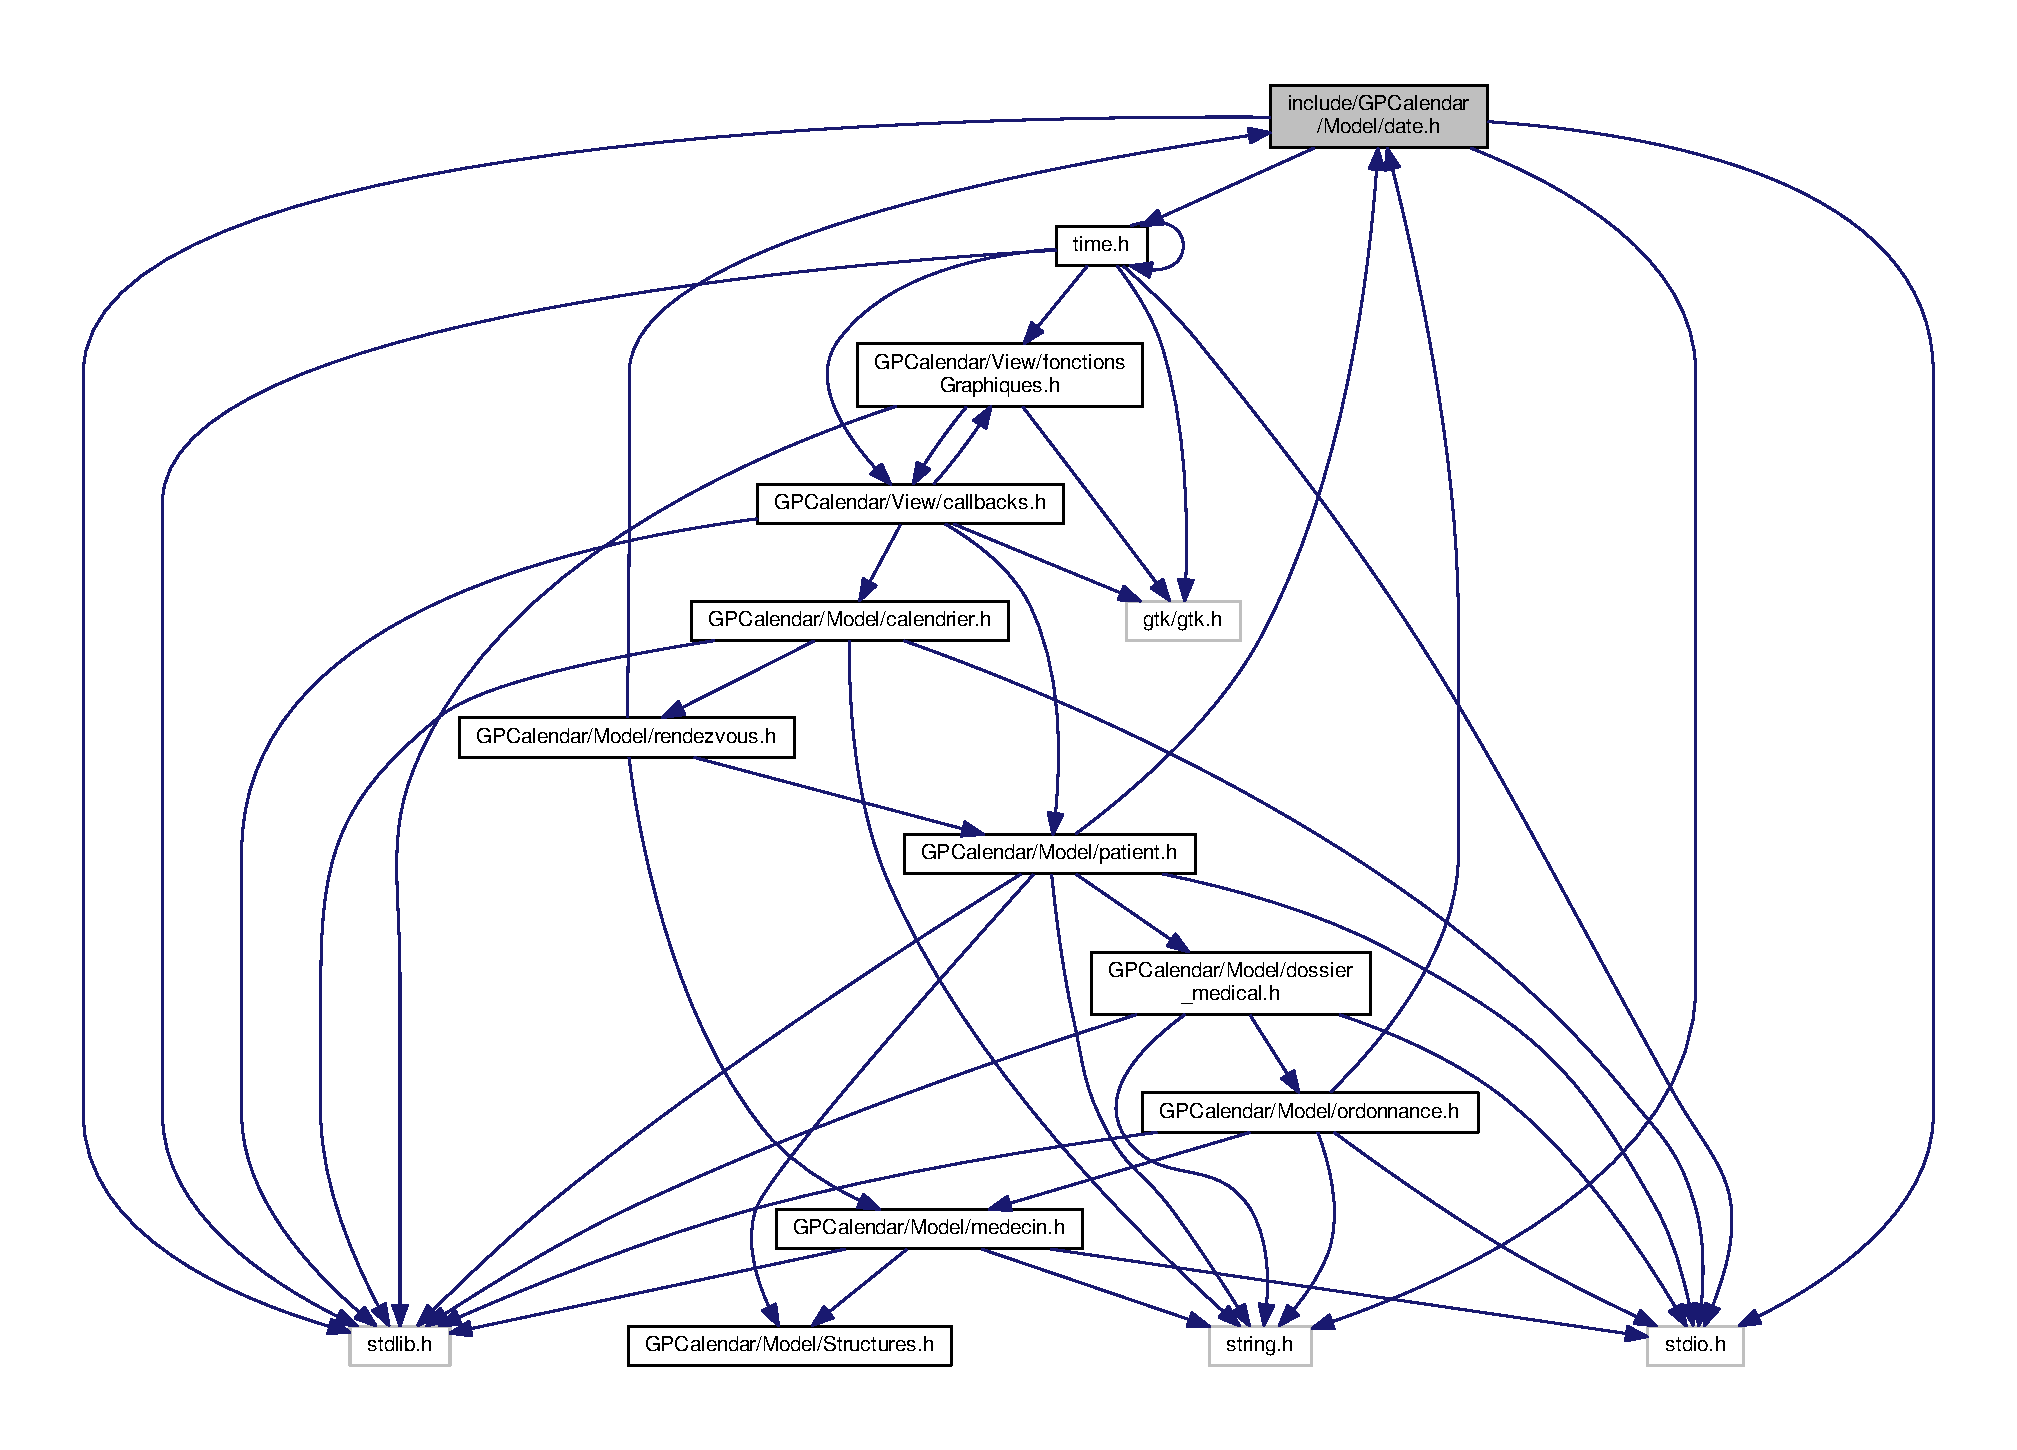
\includegraphics[width=350pt]{date_8h__incl}
\end{center}
\end{figure}
Ce graphe montre quels fichiers incluent directement ou indirectement ce fichier \-:
\nopagebreak
\begin{figure}[H]
\begin{center}
\leavevmode
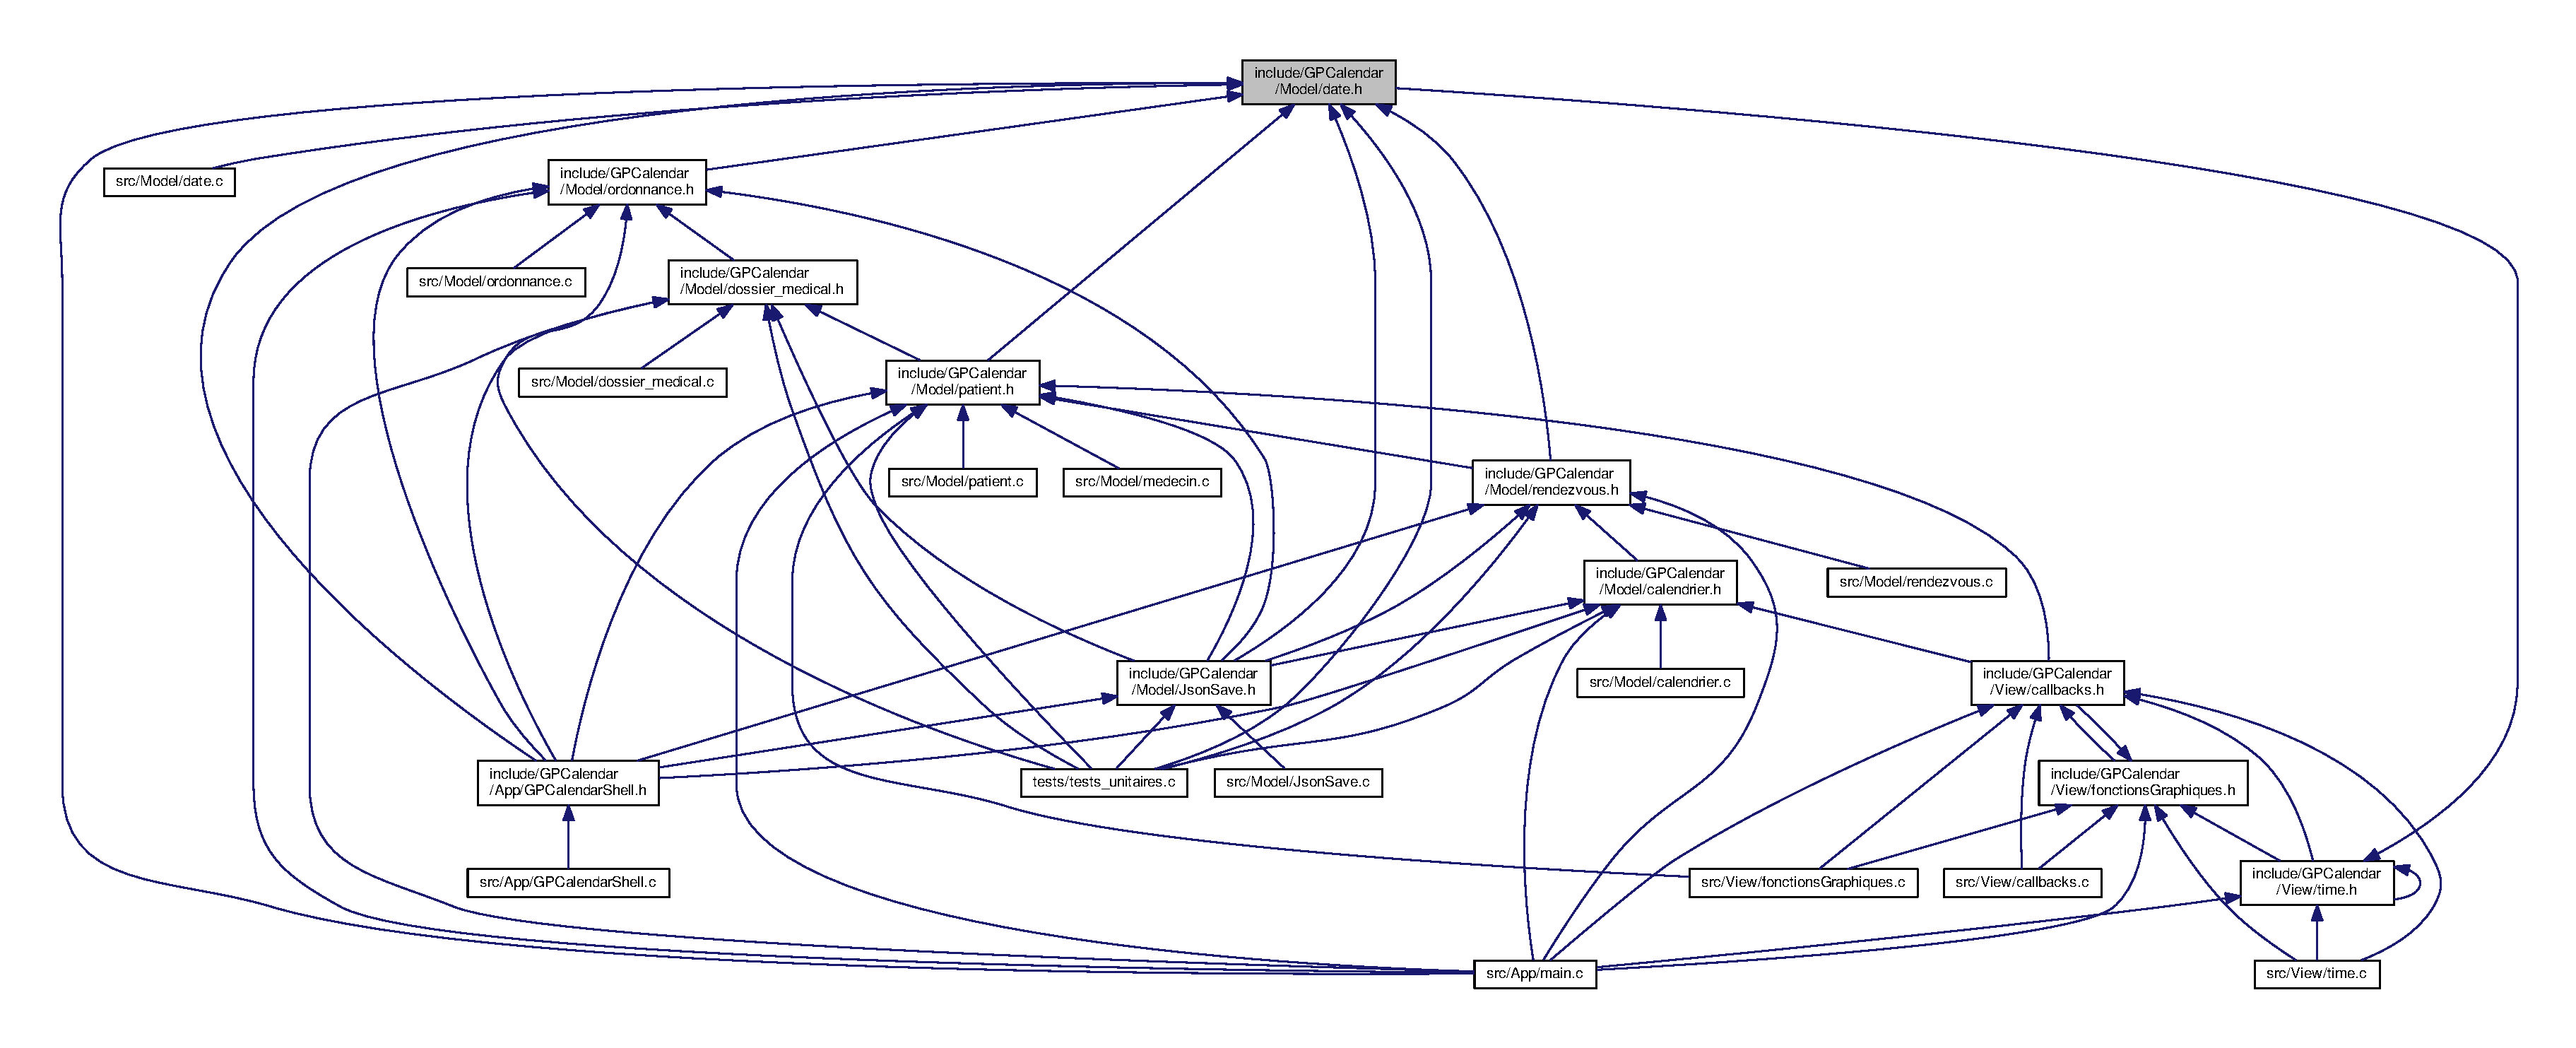
\includegraphics[width=350pt]{date_8h__dep__incl}
\end{center}
\end{figure}
\subsection*{Structures de données}
\begin{DoxyCompactItemize}
\item 
struct \hyperlink{struct_date}{Date}
\end{DoxyCompactItemize}
\subsection*{Fonctions}
\begin{DoxyCompactItemize}
\item 
\hyperlink{struct_date}{Date} $\ast$ \hyperlink{date_8h_a6b9b33d649ba9b4b0c3e906ddc194737}{Creer\-Date} (int annee, int mois, int jour)
\item 
void \hyperlink{date_8h_ab94ed681ac0fc2894d6fbf2d55582819}{Free\-Date} (\hyperlink{struct_date}{Date} $\ast$d)
\item 
\hyperlink{struct_date}{Date} $\ast$ \hyperlink{date_8h_ade26d803a4a5c87a43e1a7a7c00bb736}{Creer\-Date\-Courante} ()
\item 
\hyperlink{struct_date}{Date} $\ast$ \hyperlink{date_8h_afe0e794d1bd2a99702dedc0d86959118}{Ajout\-Mois\-Date} (\hyperlink{struct_date}{Date} $\ast$d, int nb\-\_\-mois)
\item 
void \hyperlink{date_8h_a35ba502b88e15225adc77abfdba0bbe9}{get\-Jour\-Date} (char $\ast$infos, \hyperlink{struct_date}{Date} $\ast$d)
\item 
void \hyperlink{date_8h_a2867fe49f0d396223ff7220368618c94}{get\-Mois\-Date} (char $\ast$infos, \hyperlink{struct_date}{Date} $\ast$d)
\item 
void \hyperlink{date_8h_a464fdd5871b63d8c3655b3b4723232f8}{get\-Annee\-Date} (char $\ast$infos, \hyperlink{struct_date}{Date} $\ast$d)
\item 
void \hyperlink{date_8h_aba818d6260c766df44619339e5f4ba38}{get\-Infos\-Date} (char $\ast$infos, \hyperlink{struct_date}{Date} $\ast$d)
\item 
int \hyperlink{date_8h_ac46426774b92a2898c20937e3da9097f}{Date\-Egales} (\hyperlink{struct_date}{Date} $\ast$d1, \hyperlink{struct_date}{Date} $\ast$d2)
\end{DoxyCompactItemize}


\subsection{Documentation des fonctions}
\hypertarget{date_8h_afe0e794d1bd2a99702dedc0d86959118}{\index{date.\-h@{date.\-h}!Ajout\-Mois\-Date@{Ajout\-Mois\-Date}}
\index{Ajout\-Mois\-Date@{Ajout\-Mois\-Date}!date.h@{date.\-h}}
\subsubsection[{Ajout\-Mois\-Date}]{\setlength{\rightskip}{0pt plus 5cm}{\bf Date}$\ast$ Ajout\-Mois\-Date (
\begin{DoxyParamCaption}
\item[{{\bf Date} $\ast$}]{d, }
\item[{int}]{nb\-\_\-mois}
\end{DoxyParamCaption}
)}}\label{date_8h_afe0e794d1bd2a99702dedc0d86959118}
Ajout\-Mois\-Date \-: Permet d'ajouter nb\-\_\-mois à une date la date (utile notamment pour les ordonnances) 
\begin{DoxyParams}{Paramètres}
{\em d} & \-: la date à laquelle on ajoute le nb de mois \\
\hline
{\em nb\-\_\-mois} & \\
\hline
\end{DoxyParams}
\begin{DoxyReturn}{Renvoie}
la date + nb\-\_\-mois 
\end{DoxyReturn}
\hypertarget{date_8h_a6b9b33d649ba9b4b0c3e906ddc194737}{\index{date.\-h@{date.\-h}!Creer\-Date@{Creer\-Date}}
\index{Creer\-Date@{Creer\-Date}!date.h@{date.\-h}}
\subsubsection[{Creer\-Date}]{\setlength{\rightskip}{0pt plus 5cm}{\bf Date}$\ast$ Creer\-Date (
\begin{DoxyParamCaption}
\item[{int}]{annee, }
\item[{int}]{mois, }
\item[{int}]{jour}
\end{DoxyParamCaption}
)}}\label{date_8h_a6b9b33d649ba9b4b0c3e906ddc194737}
Creer\-Date \-: Creer dynamiquement un objet \hyperlink{struct_date}{Date} 
\begin{DoxyParams}{Paramètres}
{\em annee} & \-: l'annee de cette date \\
\hline
{\em mois} & \-: le mois \\
\hline
{\em jour} & \-: le jour \\
\hline
\end{DoxyParams}
\begin{DoxyReturn}{Renvoie}
la date créée 
\end{DoxyReturn}
\hypertarget{date_8h_ade26d803a4a5c87a43e1a7a7c00bb736}{\index{date.\-h@{date.\-h}!Creer\-Date\-Courante@{Creer\-Date\-Courante}}
\index{Creer\-Date\-Courante@{Creer\-Date\-Courante}!date.h@{date.\-h}}
\subsubsection[{Creer\-Date\-Courante}]{\setlength{\rightskip}{0pt plus 5cm}{\bf Date}$\ast$ Creer\-Date\-Courante (
\begin{DoxyParamCaption}
{}
\end{DoxyParamCaption}
)}}\label{date_8h_ade26d803a4a5c87a43e1a7a7c00bb736}
Date\-Courante \-: Créer une date correspondant à la date courante \begin{DoxyReturn}{Renvoie}
la date courante 
\end{DoxyReturn}
\hypertarget{date_8h_ac46426774b92a2898c20937e3da9097f}{\index{date.\-h@{date.\-h}!Date\-Egales@{Date\-Egales}}
\index{Date\-Egales@{Date\-Egales}!date.h@{date.\-h}}
\subsubsection[{Date\-Egales}]{\setlength{\rightskip}{0pt plus 5cm}int Date\-Egales (
\begin{DoxyParamCaption}
\item[{{\bf Date} $\ast$}]{d1, }
\item[{{\bf Date} $\ast$}]{d2}
\end{DoxyParamCaption}
)}}\label{date_8h_ac46426774b92a2898c20937e3da9097f}
Date\-Egales \-: Fonction qui compare 2 dates, dit qu'elles sont égales si leur année, leur mois et leur jours sont les mêmes 
\begin{DoxyParams}{Paramètres}
{\em d1} & \-: la première date à comparer \\
\hline
{\em d2} & \-: la 2eme date \\
\hline
\end{DoxyParams}
\begin{DoxyReturn}{Renvoie}
1 si les dates sont les mêmes 0 si elles ne le sont pas -\/1 si l'une des dates est N\-U\-L\-L 
\end{DoxyReturn}
\hypertarget{date_8h_ab94ed681ac0fc2894d6fbf2d55582819}{\index{date.\-h@{date.\-h}!Free\-Date@{Free\-Date}}
\index{Free\-Date@{Free\-Date}!date.h@{date.\-h}}
\subsubsection[{Free\-Date}]{\setlength{\rightskip}{0pt plus 5cm}void Free\-Date (
\begin{DoxyParamCaption}
\item[{{\bf Date} $\ast$}]{d}
\end{DoxyParamCaption}
)}}\label{date_8h_ab94ed681ac0fc2894d6fbf2d55582819}
Free\-Date \-: Libère la mémoire d'une instance \hyperlink{struct_date}{Date} 
\begin{DoxyParams}{Paramètres}
{\em d} & \\
\hline
\end{DoxyParams}
\hypertarget{date_8h_a464fdd5871b63d8c3655b3b4723232f8}{\index{date.\-h@{date.\-h}!get\-Annee\-Date@{get\-Annee\-Date}}
\index{get\-Annee\-Date@{get\-Annee\-Date}!date.h@{date.\-h}}
\subsubsection[{get\-Annee\-Date}]{\setlength{\rightskip}{0pt plus 5cm}void get\-Annee\-Date (
\begin{DoxyParamCaption}
\item[{char $\ast$}]{infos, }
\item[{{\bf Date} $\ast$}]{d}
\end{DoxyParamCaption}
)}}\label{date_8h_a464fdd5871b63d8c3655b3b4723232f8}
get\-Annee\-Date \-: Passe l'annee de la date en paramètre sous forme de string dans infos 
\begin{DoxyParams}{Paramètres}
{\em infos} & \-: l'annee de la date sous forme de string \\
\hline
{\em d} & \-: la date dont on veut l'annee \\
\hline
\end{DoxyParams}
\hypertarget{date_8h_aba818d6260c766df44619339e5f4ba38}{\index{date.\-h@{date.\-h}!get\-Infos\-Date@{get\-Infos\-Date}}
\index{get\-Infos\-Date@{get\-Infos\-Date}!date.h@{date.\-h}}
\subsubsection[{get\-Infos\-Date}]{\setlength{\rightskip}{0pt plus 5cm}void get\-Infos\-Date (
\begin{DoxyParamCaption}
\item[{char $\ast$}]{infos, }
\item[{{\bf Date} $\ast$}]{d}
\end{DoxyParamCaption}
)}}\label{date_8h_aba818d6260c766df44619339e5f4ba38}
get\-Infos\-Date \-: Passe la date en paramètre sous forme de string X\-X/\-X\-X/\-X\-X\-X\-X dans infos 
\begin{DoxyParams}{Paramètres}
{\em infos} & \-: le jour/le mois/l'annee de la date sous forme de string \\
\hline
{\em d} & \-: la date dont on veut les infos \\
\hline
\end{DoxyParams}
\hypertarget{date_8h_a35ba502b88e15225adc77abfdba0bbe9}{\index{date.\-h@{date.\-h}!get\-Jour\-Date@{get\-Jour\-Date}}
\index{get\-Jour\-Date@{get\-Jour\-Date}!date.h@{date.\-h}}
\subsubsection[{get\-Jour\-Date}]{\setlength{\rightskip}{0pt plus 5cm}void get\-Jour\-Date (
\begin{DoxyParamCaption}
\item[{char $\ast$}]{infos, }
\item[{{\bf Date} $\ast$}]{d}
\end{DoxyParamCaption}
)}}\label{date_8h_a35ba502b88e15225adc77abfdba0bbe9}
get\-Jour\-Date \-: Passe le jour de la date en paramètre sous forme de string dans infos 
\begin{DoxyParams}{Paramètres}
{\em infos} & \-: le jour de la date sous forme de string \\
\hline
{\em d} & \-: la date dont on veut le jour \\
\hline
\end{DoxyParams}
\hypertarget{date_8h_a2867fe49f0d396223ff7220368618c94}{\index{date.\-h@{date.\-h}!get\-Mois\-Date@{get\-Mois\-Date}}
\index{get\-Mois\-Date@{get\-Mois\-Date}!date.h@{date.\-h}}
\subsubsection[{get\-Mois\-Date}]{\setlength{\rightskip}{0pt plus 5cm}void get\-Mois\-Date (
\begin{DoxyParamCaption}
\item[{char $\ast$}]{infos, }
\item[{{\bf Date} $\ast$}]{d}
\end{DoxyParamCaption}
)}}\label{date_8h_a2867fe49f0d396223ff7220368618c94}
get\-Mois\-Date \-: Passe le mois de la date en paramètre sous forme de string dans infos 
\begin{DoxyParams}{Paramètres}
{\em infos} & \-: le mois de la date sous forme de string \\
\hline
{\em d} & \-: la date dont on veut le mois \\
\hline
\end{DoxyParams}

\hypertarget{dossier__medical_8h}{\section{Référence du fichier include/\-G\-P\-Calendar/\-Model/dossier\-\_\-medical.h}
\label{dossier__medical_8h}\index{include/\-G\-P\-Calendar/\-Model/dossier\-\_\-medical.\-h@{include/\-G\-P\-Calendar/\-Model/dossier\-\_\-medical.\-h}}
}
{\ttfamily \#include \char`\"{}G\-P\-Calendar/\-Model/ordonnance.\-h\char`\"{}}\\*
{\ttfamily \#include $<$string.\-h$>$}\\*
{\ttfamily \#include $<$stdlib.\-h$>$}\\*
{\ttfamily \#include $<$stdio.\-h$>$}\\*
Graphe des dépendances par inclusion de dossier\-\_\-medical.\-h\-:
\nopagebreak
\begin{figure}[H]
\begin{center}
\leavevmode
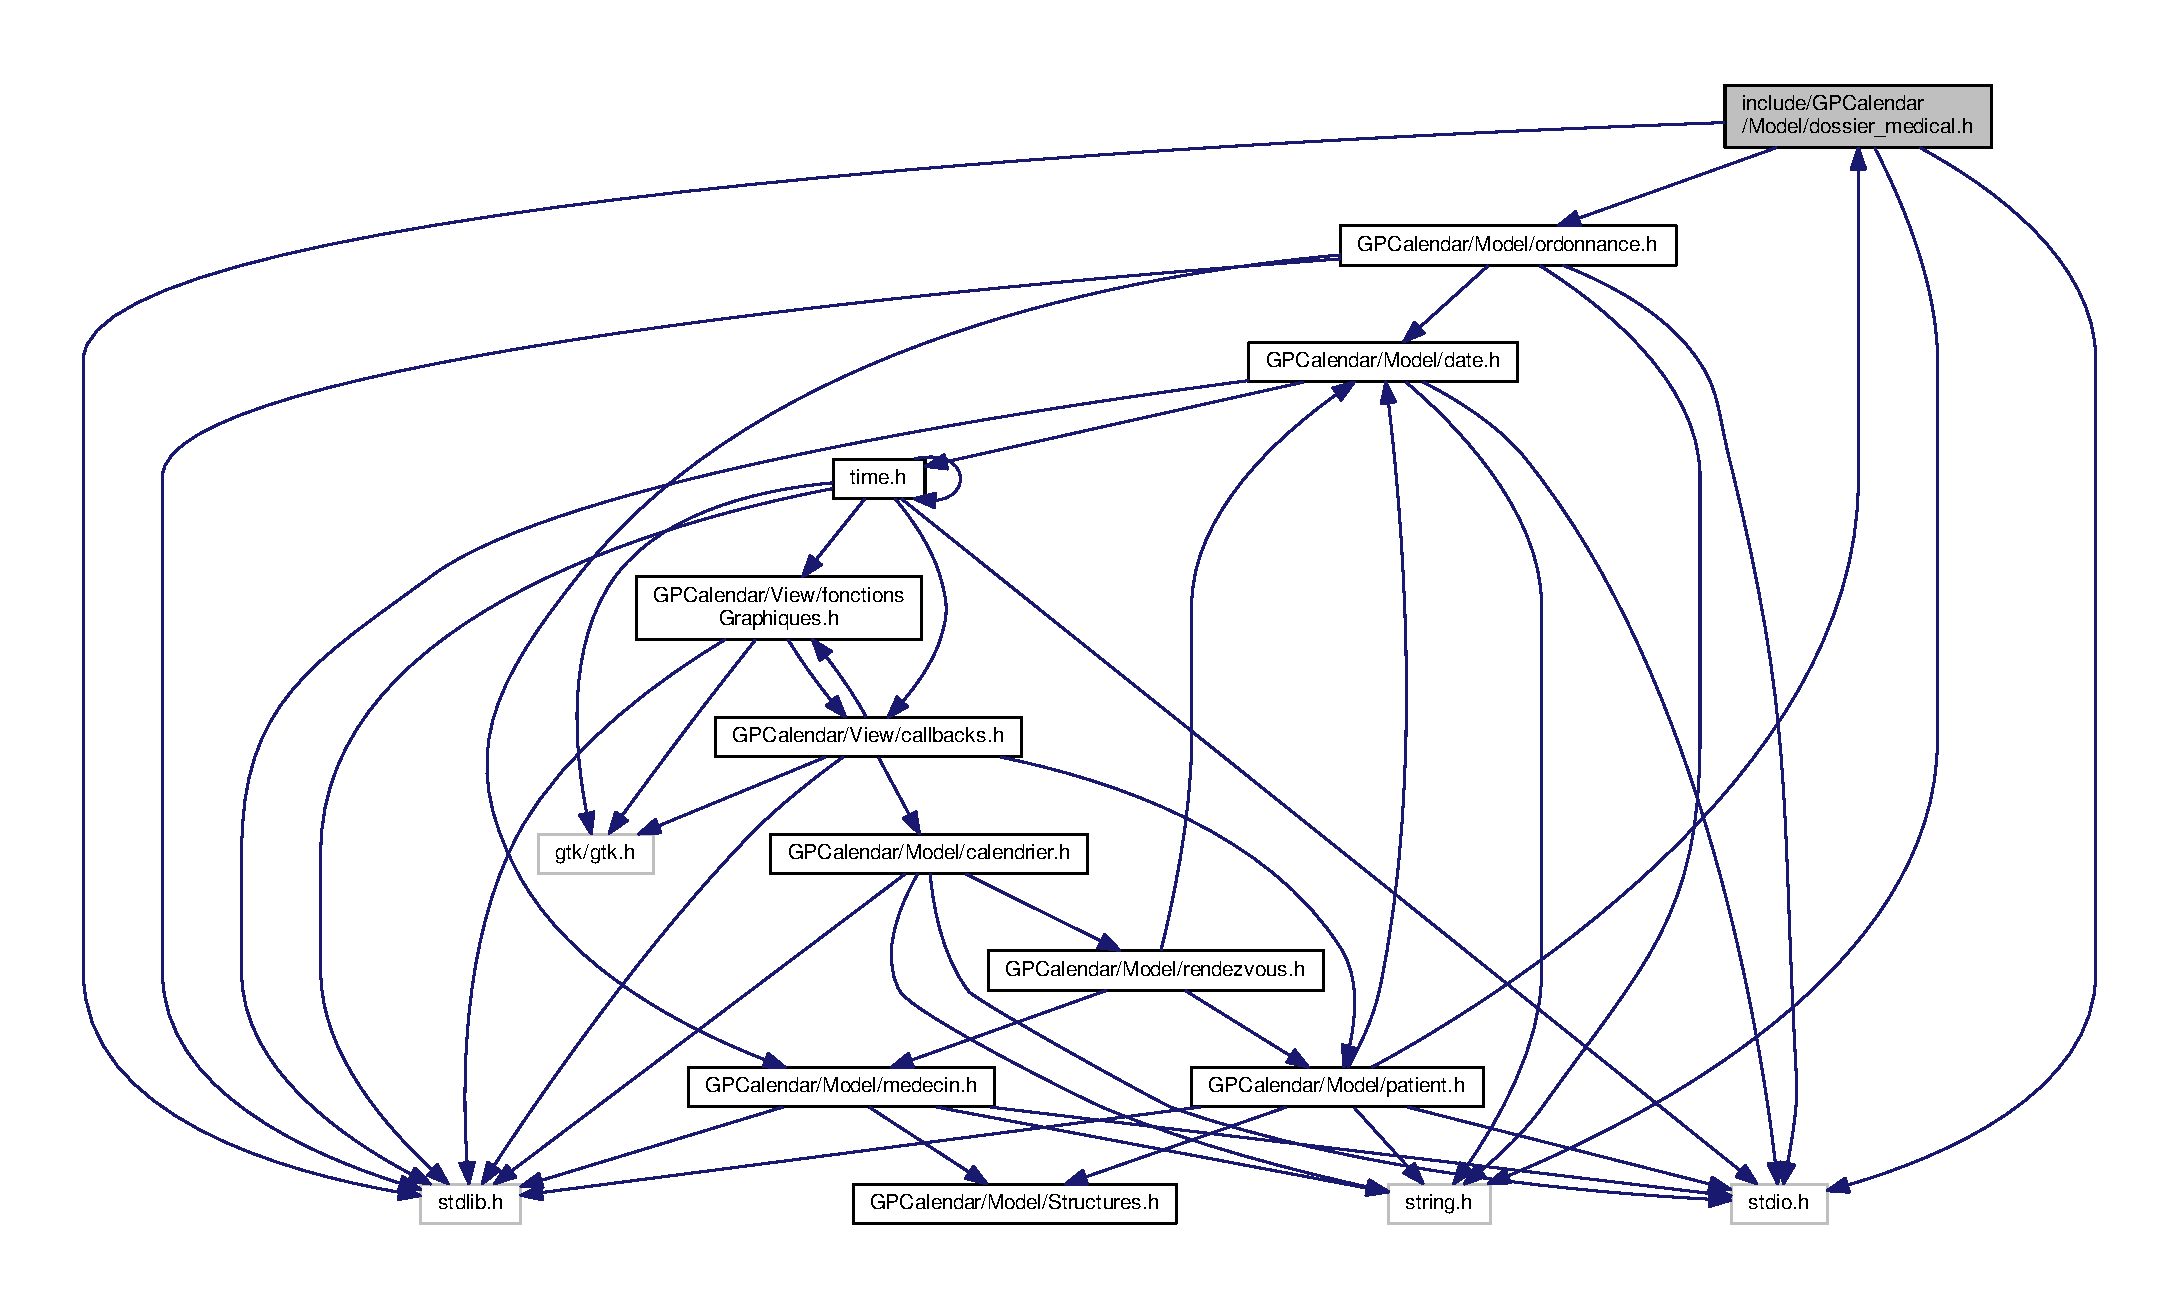
\includegraphics[width=350pt]{dossier__medical_8h__incl}
\end{center}
\end{figure}
Ce graphe montre quels fichiers incluent directement ou indirectement ce fichier \-:
\nopagebreak
\begin{figure}[H]
\begin{center}
\leavevmode
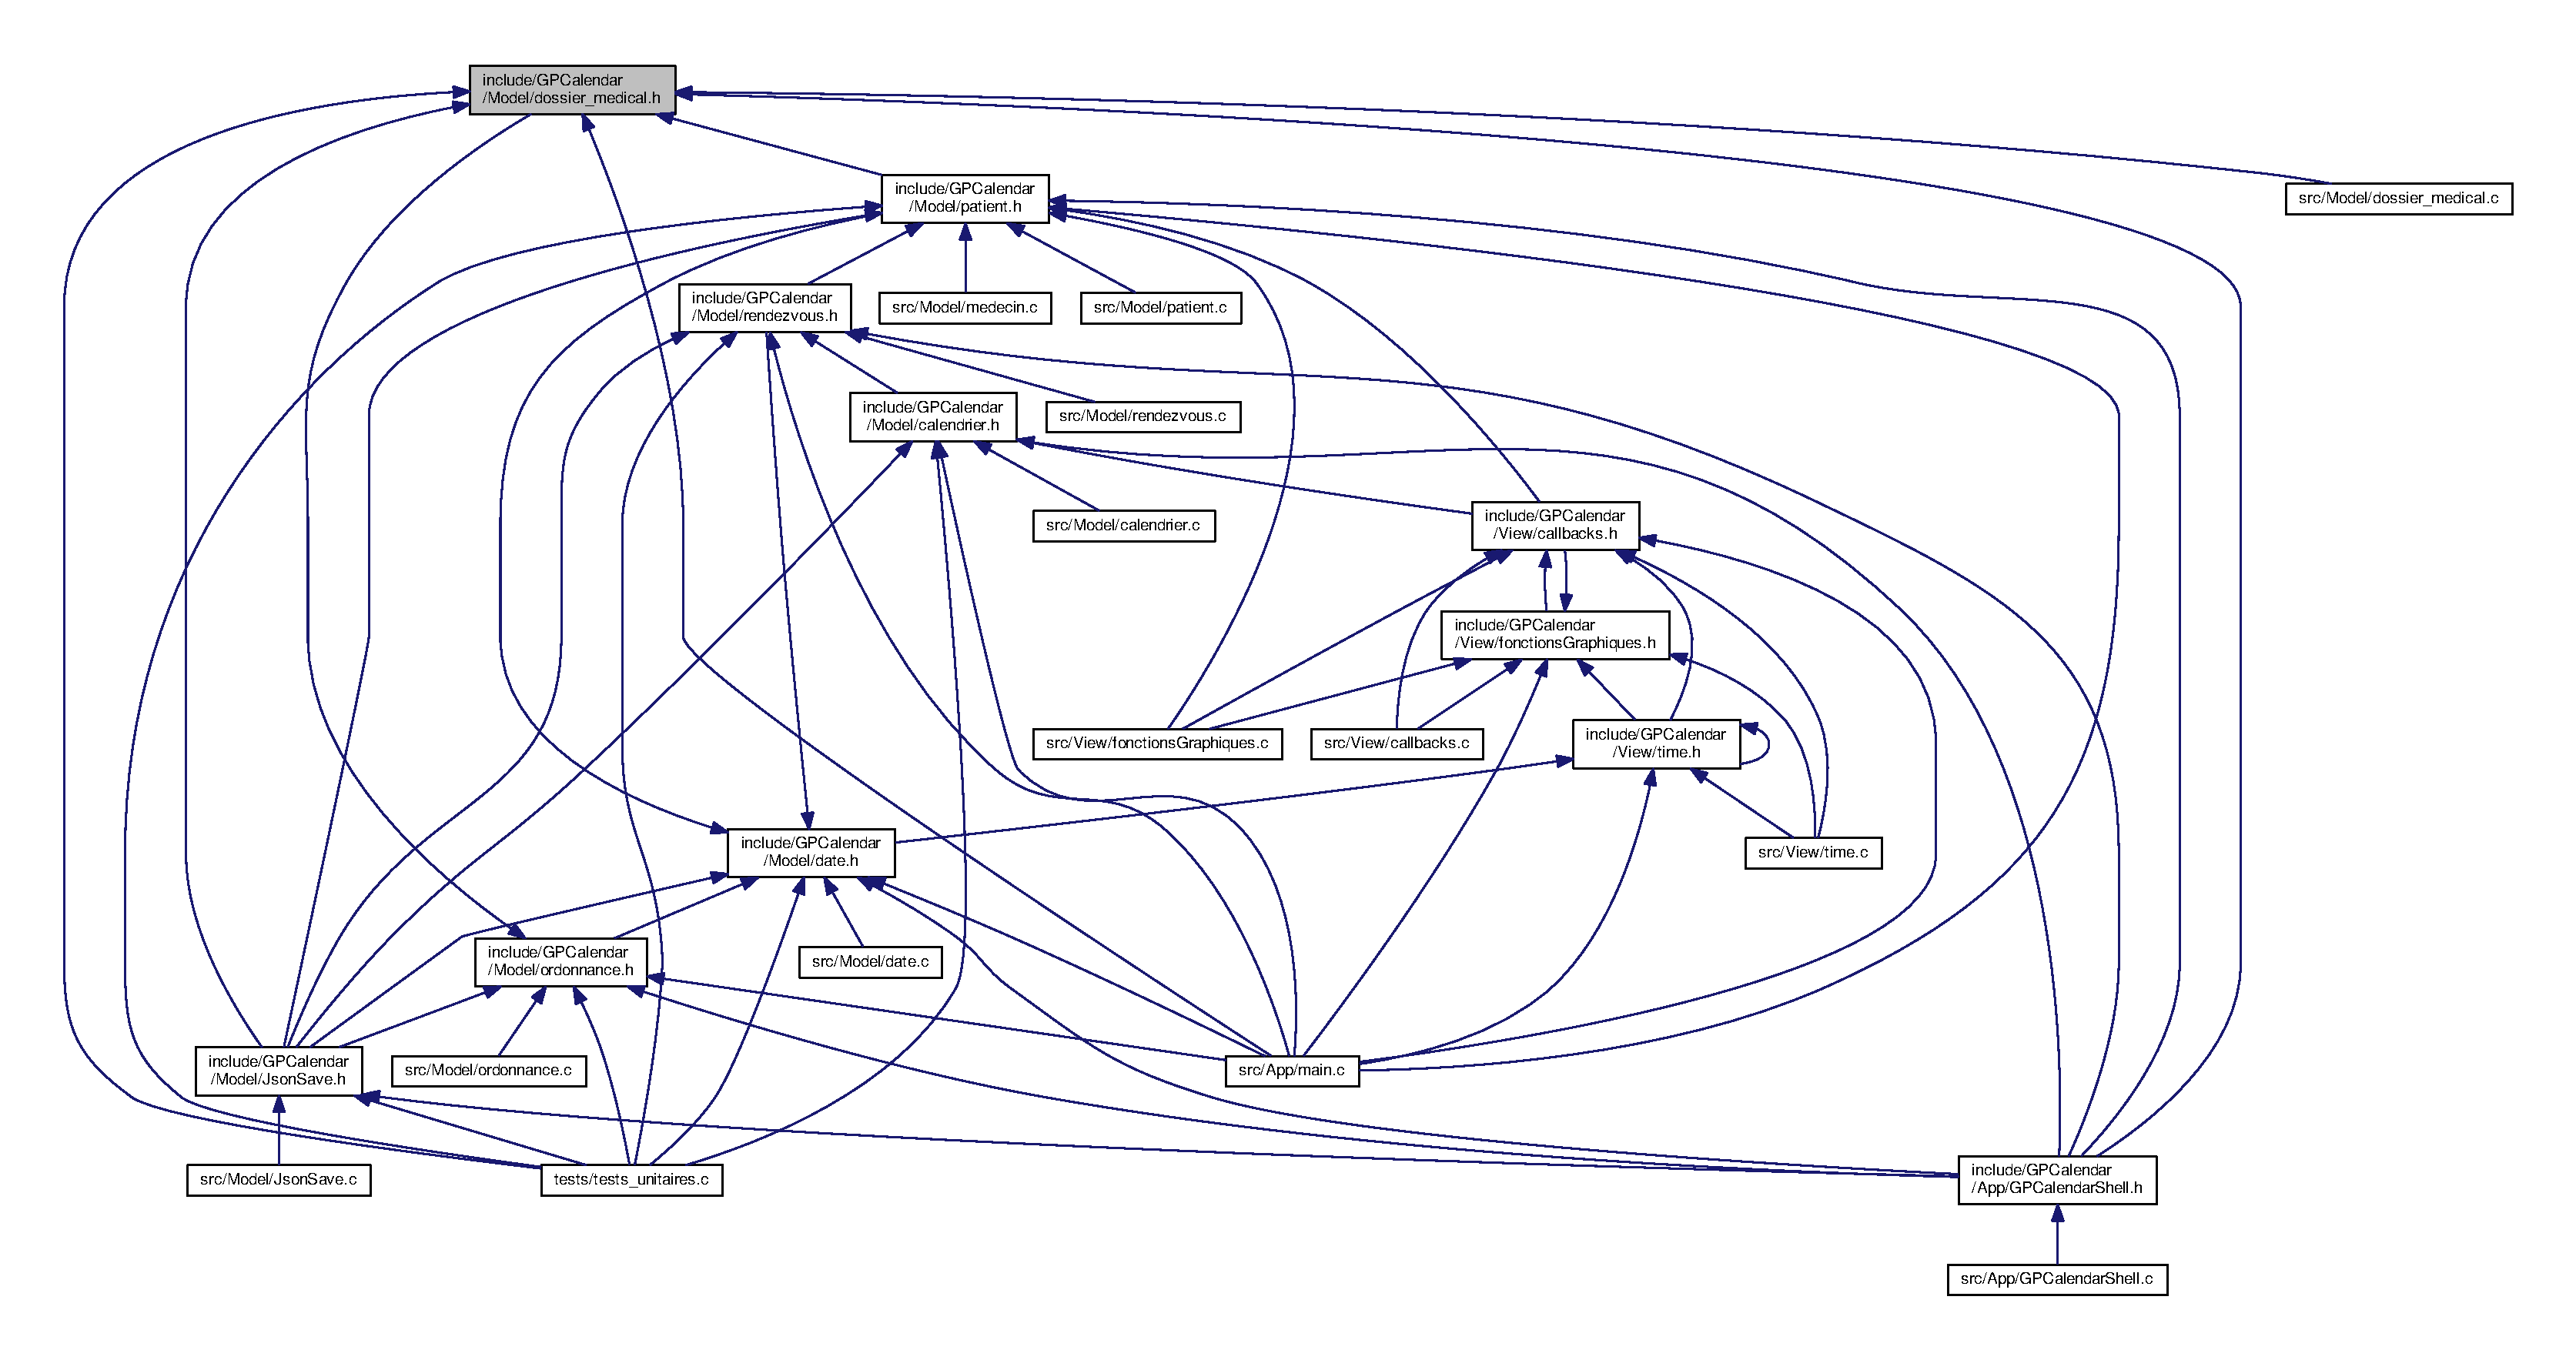
\includegraphics[width=350pt]{dossier__medical_8h__dep__incl}
\end{center}
\end{figure}
\subsection*{Structures de données}
\begin{DoxyCompactItemize}
\item 
struct \hyperlink{struct_dossier_medical}{Dossier\-Medical}
\item 
struct \hyperlink{struct_node_antecedent}{Node\-Antecedent}
\item 
struct \hyperlink{struct_list_antecedent}{List\-Antecedent}
\end{DoxyCompactItemize}
\subsection*{Définitions de type}
\begin{DoxyCompactItemize}
\item 
typedef struct \hyperlink{struct_list_antecedent}{List\-Antecedent} \hyperlink{dossier__medical_8h_ad590923d4faca35e5c8562d4d5bb4f9e}{List\-Antecedent}
\item 
typedef struct \hyperlink{struct_dossier_medical}{Dossier\-Medical} \hyperlink{dossier__medical_8h_a482d7a373d53af45b6a8db312bbda0e7}{Dossier\-Medical}
\item 
typedef struct \hyperlink{struct_node_antecedent}{Node\-Antecedent} \hyperlink{dossier__medical_8h_a95553c64bb16e0c3c92e5062729e8ca7}{Node\-Antecedent}
\end{DoxyCompactItemize}
\subsection*{Fonctions}
\begin{DoxyCompactItemize}
\item 
\hyperlink{struct_dossier_medical}{Dossier\-Medical} $\ast$ \hyperlink{dossier__medical_8h_a1db3210daf71ff58dc58d74d5a07bf62}{Creer\-Dossier\-Medical} ()
\item 
void \hyperlink{dossier__medical_8h_a44e63b91f9635db243b80de6b39e1d18}{Free\-Dossier\-Medical} (\hyperlink{struct_dossier_medical}{Dossier\-Medical} $\ast$d)
\item 
void \hyperlink{dossier__medical_8h_a9c215f91e9233e56eba1e278ee6ffb0d}{Acces\-Dossier} (\hyperlink{struct_patient}{Patient} $\ast$p)
\item 
int \hyperlink{dossier__medical_8h_a055a11ab5b446aff1ea072b18e0b0c80}{Add\-Ordonnance\-Dossier\-Medical} (\hyperlink{struct_dossier_medical}{Dossier\-Medical} $\ast$dm, \hyperlink{struct_ordonnance}{Ordonnance} $\ast$ordonnance)
\item 
int \hyperlink{dossier__medical_8h_aca624d76847984c3ab23fb8f4087527c}{Add\-Antecedent\-Dossier\-Medical} (\hyperlink{struct_dossier_medical}{Dossier\-Medical} $\ast$dm, char $\ast$ant)
\item 
void \hyperlink{dossier__medical_8h_a8e4a0090325fda62a95dacf809982593}{print\-Antecedent} (char $\ast$infos, char $\ast$ante)
\item 
\hyperlink{struct_node_antecedent}{Node\-Antecedent} $\ast$ \hyperlink{dossier__medical_8h_ac8a65401429da15e4e5438c27f1d5bc7}{new\-Node\-Antecedent} (char $\ast$ante, \hyperlink{struct_node_antecedent}{Node\-Antecedent} $\ast$previous, \hyperlink{struct_node_antecedent}{Node\-Antecedent} $\ast$next)
\item 
void \hyperlink{dossier__medical_8h_a0fca73fc369dd709c14e7de2682ec7da}{free\-Node\-Antecedent} (\hyperlink{struct_list_antecedent}{List\-Antecedent} $\ast$l, \hyperlink{struct_node_antecedent}{Node\-Antecedent} $\ast$n)
\item 
void \hyperlink{dossier__medical_8h_a85174cddd32f52cb915ce0dc1f67af77}{List\-Antecedent\-\_\-init} (\hyperlink{struct_list_antecedent}{List\-Antecedent} $\ast$l)
\item 
void \hyperlink{dossier__medical_8h_aeb097f92ae54258f575ef3d1a548b4a2}{List\-Antecedent\-\_\-free} (\hyperlink{struct_list_antecedent}{List\-Antecedent} $\ast$l)
\item 
int \hyperlink{dossier__medical_8h_a45c487156c6665f976e3bd236d33a20d}{List\-Antecedent\-\_\-is\-Empty} (\hyperlink{struct_list_antecedent}{List\-Antecedent} $\ast$l)
\item 
int \hyperlink{dossier__medical_8h_a31102bf36a7cb7b42f3e1dac1f6f941b}{List\-Antecedent\-\_\-is\-First} (\hyperlink{struct_list_antecedent}{List\-Antecedent} $\ast$l)
\item 
int \hyperlink{dossier__medical_8h_a7266fb96edb1bc50da80ec5d82b17f70}{List\-Antecedent\-\_\-is\-Last} (\hyperlink{struct_list_antecedent}{List\-Antecedent} $\ast$l)
\item 
int \hyperlink{dossier__medical_8h_af42338122c4597a30b844ca68996c1aa}{List\-Antecedent\-\_\-is\-Out\-Of\-List} (\hyperlink{struct_list_antecedent}{List\-Antecedent} $\ast$l)
\item 
void \hyperlink{dossier__medical_8h_a31fd0b56dd2cc3875a0fcb1313495f3c}{List\-Antecedent\-\_\-set\-On\-First} (\hyperlink{struct_list_antecedent}{List\-Antecedent} $\ast$l)
\item 
void \hyperlink{dossier__medical_8h_a8a564a91ea100e308d68a53db7aee9fc}{List\-Antecedent\-\_\-set\-On\-Last} (\hyperlink{struct_list_antecedent}{List\-Antecedent} $\ast$l)
\item 
void \hyperlink{dossier__medical_8h_a6905d735ace0ed3489d72c8fbd677238}{List\-Antecedent\-\_\-set\-On\-Next} (\hyperlink{struct_list_antecedent}{List\-Antecedent} $\ast$l)
\item 
void \hyperlink{dossier__medical_8h_a4269123aeb4a2223826fd39e74cdf90f}{List\-Antecedent\-\_\-set\-On\-Previous} (\hyperlink{struct_list_antecedent}{List\-Antecedent} $\ast$l)
\item 
char $\ast$ \hyperlink{dossier__medical_8h_a7d4086d62ff250c2f21718b1fb690d03}{List\-Antecedent\-\_\-get\-Current} (\hyperlink{struct_list_antecedent}{List\-Antecedent} $\ast$l)
\end{DoxyCompactItemize}


\subsection{Documentation des définitions de type}
\hypertarget{dossier__medical_8h_a482d7a373d53af45b6a8db312bbda0e7}{\index{dossier\-\_\-medical.\-h@{dossier\-\_\-medical.\-h}!Dossier\-Medical@{Dossier\-Medical}}
\index{Dossier\-Medical@{Dossier\-Medical}!dossier_medical.h@{dossier\-\_\-medical.\-h}}
\subsubsection[{Dossier\-Medical}]{\setlength{\rightskip}{0pt plus 5cm}typedef struct {\bf Dossier\-Medical} {\bf Dossier\-Medical}}}\label{dossier__medical_8h_a482d7a373d53af45b6a8db312bbda0e7}
\hypertarget{dossier__medical_8h_ad590923d4faca35e5c8562d4d5bb4f9e}{\index{dossier\-\_\-medical.\-h@{dossier\-\_\-medical.\-h}!List\-Antecedent@{List\-Antecedent}}
\index{List\-Antecedent@{List\-Antecedent}!dossier_medical.h@{dossier\-\_\-medical.\-h}}
\subsubsection[{List\-Antecedent}]{\setlength{\rightskip}{0pt plus 5cm}typedef struct {\bf List\-Antecedent} {\bf List\-Antecedent}}}\label{dossier__medical_8h_ad590923d4faca35e5c8562d4d5bb4f9e}
\hypertarget{dossier__medical_8h_a95553c64bb16e0c3c92e5062729e8ca7}{\index{dossier\-\_\-medical.\-h@{dossier\-\_\-medical.\-h}!Node\-Antecedent@{Node\-Antecedent}}
\index{Node\-Antecedent@{Node\-Antecedent}!dossier_medical.h@{dossier\-\_\-medical.\-h}}
\subsubsection[{Node\-Antecedent}]{\setlength{\rightskip}{0pt plus 5cm}typedef struct {\bf Node\-Antecedent} {\bf Node\-Antecedent}}}\label{dossier__medical_8h_a95553c64bb16e0c3c92e5062729e8ca7}
Structure \hyperlink{struct_node_antecedent}{Node\-Antecedent} 

\subsection{Documentation des fonctions}
\hypertarget{dossier__medical_8h_a9c215f91e9233e56eba1e278ee6ffb0d}{\index{dossier\-\_\-medical.\-h@{dossier\-\_\-medical.\-h}!Acces\-Dossier@{Acces\-Dossier}}
\index{Acces\-Dossier@{Acces\-Dossier}!dossier_medical.h@{dossier\-\_\-medical.\-h}}
\subsubsection[{Acces\-Dossier}]{\setlength{\rightskip}{0pt plus 5cm}void Acces\-Dossier (
\begin{DoxyParamCaption}
\item[{{\bf Patient} $\ast$}]{p}
\end{DoxyParamCaption}
)}}\label{dossier__medical_8h_a9c215f91e9233e56eba1e278ee6ffb0d}
\hypertarget{dossier__medical_8h_aca624d76847984c3ab23fb8f4087527c}{\index{dossier\-\_\-medical.\-h@{dossier\-\_\-medical.\-h}!Add\-Antecedent\-Dossier\-Medical@{Add\-Antecedent\-Dossier\-Medical}}
\index{Add\-Antecedent\-Dossier\-Medical@{Add\-Antecedent\-Dossier\-Medical}!dossier_medical.h@{dossier\-\_\-medical.\-h}}
\subsubsection[{Add\-Antecedent\-Dossier\-Medical}]{\setlength{\rightskip}{0pt plus 5cm}int Add\-Antecedent\-Dossier\-Medical (
\begin{DoxyParamCaption}
\item[{{\bf Dossier\-Medical} $\ast$}]{dm, }
\item[{char $\ast$}]{ant}
\end{DoxyParamCaption}
)}}\label{dossier__medical_8h_aca624d76847984c3ab23fb8f4087527c}
Add\-Antecedent\-Dossier\-Medical \-: Ajoute un antecedent dans le dossier medical 
\begin{DoxyParams}{Paramètres}
{\em dm} & \-: le dossier dans lequel on veut ajouter \\
\hline
{\em antecedent} & \-: l'antecedent à ajouter \\
\hline
\end{DoxyParams}
\hypertarget{dossier__medical_8h_a055a11ab5b446aff1ea072b18e0b0c80}{\index{dossier\-\_\-medical.\-h@{dossier\-\_\-medical.\-h}!Add\-Ordonnance\-Dossier\-Medical@{Add\-Ordonnance\-Dossier\-Medical}}
\index{Add\-Ordonnance\-Dossier\-Medical@{Add\-Ordonnance\-Dossier\-Medical}!dossier_medical.h@{dossier\-\_\-medical.\-h}}
\subsubsection[{Add\-Ordonnance\-Dossier\-Medical}]{\setlength{\rightskip}{0pt plus 5cm}int Add\-Ordonnance\-Dossier\-Medical (
\begin{DoxyParamCaption}
\item[{{\bf Dossier\-Medical} $\ast$}]{dm, }
\item[{{\bf Ordonnance} $\ast$}]{ordonnance}
\end{DoxyParamCaption}
)}}\label{dossier__medical_8h_a055a11ab5b446aff1ea072b18e0b0c80}
Add\-Ordonnance\-Dossier\-Medical \-: Ajoute une ordonnance dans le dossier medical 
\begin{DoxyParams}{Paramètres}
{\em dm} & \-: le dossier dans lequel on veut ajouter \\
\hline
{\em ordonnance} & \-: l'ordonnance à ajouter \\
\hline
\end{DoxyParams}
\hypertarget{dossier__medical_8h_a1db3210daf71ff58dc58d74d5a07bf62}{\index{dossier\-\_\-medical.\-h@{dossier\-\_\-medical.\-h}!Creer\-Dossier\-Medical@{Creer\-Dossier\-Medical}}
\index{Creer\-Dossier\-Medical@{Creer\-Dossier\-Medical}!dossier_medical.h@{dossier\-\_\-medical.\-h}}
\subsubsection[{Creer\-Dossier\-Medical}]{\setlength{\rightskip}{0pt plus 5cm}{\bf Dossier\-Medical}$\ast$ Creer\-Dossier\-Medical (
\begin{DoxyParamCaption}
{}
\end{DoxyParamCaption}
)}}\label{dossier__medical_8h_a1db3210daf71ff58dc58d74d5a07bf62}
Creer\-Dossier \-: Creer dynamiquement un objet \hyperlink{struct_dossier_medical}{Dossier\-Medical} 
\begin{DoxyParams}{Paramètres}
{\em patient} & \-: le patient concerné par le dossier \\
\hline
\end{DoxyParams}
\begin{DoxyReturn}{Renvoie}
le dossier crée 
\end{DoxyReturn}
\hypertarget{dossier__medical_8h_a44e63b91f9635db243b80de6b39e1d18}{\index{dossier\-\_\-medical.\-h@{dossier\-\_\-medical.\-h}!Free\-Dossier\-Medical@{Free\-Dossier\-Medical}}
\index{Free\-Dossier\-Medical@{Free\-Dossier\-Medical}!dossier_medical.h@{dossier\-\_\-medical.\-h}}
\subsubsection[{Free\-Dossier\-Medical}]{\setlength{\rightskip}{0pt plus 5cm}void Free\-Dossier\-Medical (
\begin{DoxyParamCaption}
\item[{{\bf Dossier\-Medical} $\ast$}]{dm}
\end{DoxyParamCaption}
)}}\label{dossier__medical_8h_a44e63b91f9635db243b80de6b39e1d18}
Free\-Dossier \-: Free un objet \hyperlink{struct_dossier_medical}{Dossier\-Medical} 
\begin{DoxyParams}{Paramètres}
{\em dm} & \-: le dossier à supprimer \\
\hline
\end{DoxyParams}
\hypertarget{dossier__medical_8h_a0fca73fc369dd709c14e7de2682ec7da}{\index{dossier\-\_\-medical.\-h@{dossier\-\_\-medical.\-h}!free\-Node\-Antecedent@{free\-Node\-Antecedent}}
\index{free\-Node\-Antecedent@{free\-Node\-Antecedent}!dossier_medical.h@{dossier\-\_\-medical.\-h}}
\subsubsection[{free\-Node\-Antecedent}]{\setlength{\rightskip}{0pt plus 5cm}void free\-Node\-Antecedent (
\begin{DoxyParamCaption}
\item[{{\bf List\-Antecedent} $\ast$}]{l, }
\item[{{\bf Node\-Antecedent} $\ast$}]{n}
\end{DoxyParamCaption}
)}}\label{dossier__medical_8h_a0fca73fc369dd709c14e7de2682ec7da}
free\-Node\-Antecedent \-: Permet de delete proprement (avec un free) un \hyperlink{struct_node_antecedent}{Node\-Antecedent} 
\begin{DoxyParams}{Paramètres}
{\em n} & \-: le node à delete \\
\hline
\end{DoxyParams}
\hypertarget{dossier__medical_8h_aeb097f92ae54258f575ef3d1a548b4a2}{\index{dossier\-\_\-medical.\-h@{dossier\-\_\-medical.\-h}!List\-Antecedent\-\_\-free@{List\-Antecedent\-\_\-free}}
\index{List\-Antecedent\-\_\-free@{List\-Antecedent\-\_\-free}!dossier_medical.h@{dossier\-\_\-medical.\-h}}
\subsubsection[{List\-Antecedent\-\_\-free}]{\setlength{\rightskip}{0pt plus 5cm}void List\-Antecedent\-\_\-free (
\begin{DoxyParamCaption}
\item[{{\bf List\-Antecedent} $\ast$}]{l}
\end{DoxyParamCaption}
)}}\label{dossier__medical_8h_aeb097f92ae54258f575ef3d1a548b4a2}
List\-Antecedent\-\_\-free \-: Libère la mémoire occupée par l'objet \hyperlink{struct_list_antecedent}{List\-Antecedent} passé en paramètre 
\begin{DoxyParams}{Paramètres}
{\em l} & \-: la liste de antecedents à free \\
\hline
\end{DoxyParams}
\hypertarget{dossier__medical_8h_a7d4086d62ff250c2f21718b1fb690d03}{\index{dossier\-\_\-medical.\-h@{dossier\-\_\-medical.\-h}!List\-Antecedent\-\_\-get\-Current@{List\-Antecedent\-\_\-get\-Current}}
\index{List\-Antecedent\-\_\-get\-Current@{List\-Antecedent\-\_\-get\-Current}!dossier_medical.h@{dossier\-\_\-medical.\-h}}
\subsubsection[{List\-Antecedent\-\_\-get\-Current}]{\setlength{\rightskip}{0pt plus 5cm}char$\ast$ List\-Antecedent\-\_\-get\-Current (
\begin{DoxyParamCaption}
\item[{{\bf List\-Antecedent} $\ast$}]{l}
\end{DoxyParamCaption}
)}}\label{dossier__medical_8h_a7d4086d62ff250c2f21718b1fb690d03}
List\-Antecedent\-\_\-get\-Current \-: Permet d'acceder à l'\hyperlink{struct_ordonnance}{Ordonnance} pointée par current 
\begin{DoxyParams}{Paramètres}
{\em l} & \-: la liste \\
\hline
\end{DoxyParams}
\begin{DoxyReturn}{Renvoie}
Retourne un pointeur sur l'\hyperlink{struct_ordonnance}{Ordonnance} de l'élément courant de la liste 
\end{DoxyReturn}
\hypertarget{dossier__medical_8h_a85174cddd32f52cb915ce0dc1f67af77}{\index{dossier\-\_\-medical.\-h@{dossier\-\_\-medical.\-h}!List\-Antecedent\-\_\-init@{List\-Antecedent\-\_\-init}}
\index{List\-Antecedent\-\_\-init@{List\-Antecedent\-\_\-init}!dossier_medical.h@{dossier\-\_\-medical.\-h}}
\subsubsection[{List\-Antecedent\-\_\-init}]{\setlength{\rightskip}{0pt plus 5cm}void List\-Antecedent\-\_\-init (
\begin{DoxyParamCaption}
\item[{{\bf List\-Antecedent} $\ast$}]{l}
\end{DoxyParamCaption}
)}}\label{dossier__medical_8h_a85174cddd32f52cb915ce0dc1f67af77}
List\-Antecedent\-\_\-init \-: Initialise correctement une liste de \hyperlink{struct_node_antecedent}{Node\-Antecedent} en reliant sentinel\-\_\-begin et end entre eux et en mettant current à N\-U\-L\-L (en dehors de la liste) 
\begin{DoxyParams}{Paramètres}
{\em l} & \-: la liste à initialiser \\
\hline
\end{DoxyParams}
\hypertarget{dossier__medical_8h_a45c487156c6665f976e3bd236d33a20d}{\index{dossier\-\_\-medical.\-h@{dossier\-\_\-medical.\-h}!List\-Antecedent\-\_\-is\-Empty@{List\-Antecedent\-\_\-is\-Empty}}
\index{List\-Antecedent\-\_\-is\-Empty@{List\-Antecedent\-\_\-is\-Empty}!dossier_medical.h@{dossier\-\_\-medical.\-h}}
\subsubsection[{List\-Antecedent\-\_\-is\-Empty}]{\setlength{\rightskip}{0pt plus 5cm}int List\-Antecedent\-\_\-is\-Empty (
\begin{DoxyParamCaption}
\item[{{\bf List\-Antecedent} $\ast$}]{l}
\end{DoxyParamCaption}
)}}\label{dossier__medical_8h_a45c487156c6665f976e3bd236d33a20d}
List\-Antecedent\-\_\-is\-Empty \-: Vérifie si la liste de Antecedent est vide ou non 
\begin{DoxyParams}{Paramètres}
{\em l} & \-: la liste \\
\hline
\end{DoxyParams}
\begin{DoxyReturn}{Renvoie}
1 si la liste est vide 0 si elle ne l'est pas -\/1 si la liste est N\-U\-L\-L 
\end{DoxyReturn}
\hypertarget{dossier__medical_8h_a31102bf36a7cb7b42f3e1dac1f6f941b}{\index{dossier\-\_\-medical.\-h@{dossier\-\_\-medical.\-h}!List\-Antecedent\-\_\-is\-First@{List\-Antecedent\-\_\-is\-First}}
\index{List\-Antecedent\-\_\-is\-First@{List\-Antecedent\-\_\-is\-First}!dossier_medical.h@{dossier\-\_\-medical.\-h}}
\subsubsection[{List\-Antecedent\-\_\-is\-First}]{\setlength{\rightskip}{0pt plus 5cm}int List\-Antecedent\-\_\-is\-First (
\begin{DoxyParamCaption}
\item[{{\bf List\-Antecedent} $\ast$}]{l}
\end{DoxyParamCaption}
)}}\label{dossier__medical_8h_a31102bf36a7cb7b42f3e1dac1f6f941b}
List\-Antecedent\-\_\-is\-First \-: Vérifie si current est positionné sur le premier élément de la liste 
\begin{DoxyParams}{Paramètres}
{\em l} & \-: la liste \\
\hline
\end{DoxyParams}
\begin{DoxyReturn}{Renvoie}
1 si current est bien sur le premier élément 0 si il ne l'est pas -\/1 si la liste est N\-U\-L\-L 
\end{DoxyReturn}
\hypertarget{dossier__medical_8h_a7266fb96edb1bc50da80ec5d82b17f70}{\index{dossier\-\_\-medical.\-h@{dossier\-\_\-medical.\-h}!List\-Antecedent\-\_\-is\-Last@{List\-Antecedent\-\_\-is\-Last}}
\index{List\-Antecedent\-\_\-is\-Last@{List\-Antecedent\-\_\-is\-Last}!dossier_medical.h@{dossier\-\_\-medical.\-h}}
\subsubsection[{List\-Antecedent\-\_\-is\-Last}]{\setlength{\rightskip}{0pt plus 5cm}int List\-Antecedent\-\_\-is\-Last (
\begin{DoxyParamCaption}
\item[{{\bf List\-Antecedent} $\ast$}]{l}
\end{DoxyParamCaption}
)}}\label{dossier__medical_8h_a7266fb96edb1bc50da80ec5d82b17f70}
List\-Antecedent\-\_\-is\-Last \-: Vérifie si current est positionné sur le dernier élément de la liste 
\begin{DoxyParams}{Paramètres}
{\em l} & \-: la liste \\
\hline
\end{DoxyParams}
\begin{DoxyReturn}{Renvoie}
1 si current est bien sur le dernier élément 0 si il ne l'est pas -\/1 si la liste est N\-U\-L\-L 
\end{DoxyReturn}
\hypertarget{dossier__medical_8h_af42338122c4597a30b844ca68996c1aa}{\index{dossier\-\_\-medical.\-h@{dossier\-\_\-medical.\-h}!List\-Antecedent\-\_\-is\-Out\-Of\-List@{List\-Antecedent\-\_\-is\-Out\-Of\-List}}
\index{List\-Antecedent\-\_\-is\-Out\-Of\-List@{List\-Antecedent\-\_\-is\-Out\-Of\-List}!dossier_medical.h@{dossier\-\_\-medical.\-h}}
\subsubsection[{List\-Antecedent\-\_\-is\-Out\-Of\-List}]{\setlength{\rightskip}{0pt plus 5cm}int List\-Antecedent\-\_\-is\-Out\-Of\-List (
\begin{DoxyParamCaption}
\item[{{\bf List\-Antecedent} $\ast$}]{l}
\end{DoxyParamCaption}
)}}\label{dossier__medical_8h_af42338122c4597a30b844ca68996c1aa}
List\-Antecedent\-\_\-is\-Out\-Of\-List \-: Vérifie si current est bien placé sur un élément de la liste (les sentinels ne sont pas considérées comme dans la liste) 
\begin{DoxyParams}{Paramètres}
{\em l} & \-: la liste \\
\hline
\end{DoxyParams}
\begin{DoxyReturn}{Renvoie}
1 si current vaut N\-U\-L\-L 0 sinon -\/1 si la liste est N\-U\-L\-L 
\end{DoxyReturn}
\hypertarget{dossier__medical_8h_a31fd0b56dd2cc3875a0fcb1313495f3c}{\index{dossier\-\_\-medical.\-h@{dossier\-\_\-medical.\-h}!List\-Antecedent\-\_\-set\-On\-First@{List\-Antecedent\-\_\-set\-On\-First}}
\index{List\-Antecedent\-\_\-set\-On\-First@{List\-Antecedent\-\_\-set\-On\-First}!dossier_medical.h@{dossier\-\_\-medical.\-h}}
\subsubsection[{List\-Antecedent\-\_\-set\-On\-First}]{\setlength{\rightskip}{0pt plus 5cm}void List\-Antecedent\-\_\-set\-On\-First (
\begin{DoxyParamCaption}
\item[{{\bf List\-Antecedent} $\ast$}]{l}
\end{DoxyParamCaption}
)}}\label{dossier__medical_8h_a31fd0b56dd2cc3875a0fcb1313495f3c}
List\-Antecedent\-\_\-set\-On\-First \-: Positionne le pointeur courant sur le premier élément de la liste 
\begin{DoxyParams}{Paramètres}
{\em l} & \-: la liste \\
\hline
\end{DoxyParams}
\hypertarget{dossier__medical_8h_a8a564a91ea100e308d68a53db7aee9fc}{\index{dossier\-\_\-medical.\-h@{dossier\-\_\-medical.\-h}!List\-Antecedent\-\_\-set\-On\-Last@{List\-Antecedent\-\_\-set\-On\-Last}}
\index{List\-Antecedent\-\_\-set\-On\-Last@{List\-Antecedent\-\_\-set\-On\-Last}!dossier_medical.h@{dossier\-\_\-medical.\-h}}
\subsubsection[{List\-Antecedent\-\_\-set\-On\-Last}]{\setlength{\rightskip}{0pt plus 5cm}void List\-Antecedent\-\_\-set\-On\-Last (
\begin{DoxyParamCaption}
\item[{{\bf List\-Antecedent} $\ast$}]{l}
\end{DoxyParamCaption}
)}}\label{dossier__medical_8h_a8a564a91ea100e308d68a53db7aee9fc}
List\-Antecedent\-\_\-set\-On\-Last \-: Positionne le pointeur courant sur le dernier élément de la liste 
\begin{DoxyParams}{Paramètres}
{\em l} & \-: la liste \\
\hline
\end{DoxyParams}
\hypertarget{dossier__medical_8h_a6905d735ace0ed3489d72c8fbd677238}{\index{dossier\-\_\-medical.\-h@{dossier\-\_\-medical.\-h}!List\-Antecedent\-\_\-set\-On\-Next@{List\-Antecedent\-\_\-set\-On\-Next}}
\index{List\-Antecedent\-\_\-set\-On\-Next@{List\-Antecedent\-\_\-set\-On\-Next}!dossier_medical.h@{dossier\-\_\-medical.\-h}}
\subsubsection[{List\-Antecedent\-\_\-set\-On\-Next}]{\setlength{\rightskip}{0pt plus 5cm}void List\-Antecedent\-\_\-set\-On\-Next (
\begin{DoxyParamCaption}
\item[{{\bf List\-Antecedent} $\ast$}]{l}
\end{DoxyParamCaption}
)}}\label{dossier__medical_8h_a6905d735ace0ed3489d72c8fbd677238}
List\-Antecedent\-\_\-set\-On\-Next \-: Positionne le pointeur courant sur le prochain élément de la liste 
\begin{DoxyParams}{Paramètres}
{\em l} & \-: la liste \\
\hline
\end{DoxyParams}
\hypertarget{dossier__medical_8h_a4269123aeb4a2223826fd39e74cdf90f}{\index{dossier\-\_\-medical.\-h@{dossier\-\_\-medical.\-h}!List\-Antecedent\-\_\-set\-On\-Previous@{List\-Antecedent\-\_\-set\-On\-Previous}}
\index{List\-Antecedent\-\_\-set\-On\-Previous@{List\-Antecedent\-\_\-set\-On\-Previous}!dossier_medical.h@{dossier\-\_\-medical.\-h}}
\subsubsection[{List\-Antecedent\-\_\-set\-On\-Previous}]{\setlength{\rightskip}{0pt plus 5cm}void List\-Antecedent\-\_\-set\-On\-Previous (
\begin{DoxyParamCaption}
\item[{{\bf List\-Antecedent} $\ast$}]{l}
\end{DoxyParamCaption}
)}}\label{dossier__medical_8h_a4269123aeb4a2223826fd39e74cdf90f}
List\-Antecedent\-\_\-set\-On\-Previous \-: Positionne le pointeur courant sur l'élément le précédant dans la liste 
\begin{DoxyParams}{Paramètres}
{\em l} & \-: la liste \\
\hline
\end{DoxyParams}
\hypertarget{dossier__medical_8h_ac8a65401429da15e4e5438c27f1d5bc7}{\index{dossier\-\_\-medical.\-h@{dossier\-\_\-medical.\-h}!new\-Node\-Antecedent@{new\-Node\-Antecedent}}
\index{new\-Node\-Antecedent@{new\-Node\-Antecedent}!dossier_medical.h@{dossier\-\_\-medical.\-h}}
\subsubsection[{new\-Node\-Antecedent}]{\setlength{\rightskip}{0pt plus 5cm}{\bf Node\-Antecedent}$\ast$ new\-Node\-Antecedent (
\begin{DoxyParamCaption}
\item[{char $\ast$}]{ante, }
\item[{{\bf Node\-Antecedent} $\ast$}]{previous, }
\item[{{\bf Node\-Antecedent} $\ast$}]{next}
\end{DoxyParamCaption}
)}}\label{dossier__medical_8h_ac8a65401429da15e4e5438c27f1d5bc7}
new\-Node\-Antecedent \-: Permet de créer dynamiquement un nouveau node de Antecedent pour la liste 
\begin{DoxyParams}{Paramètres}
{\em ante} & \-: l'antecedent pointé par ce nouveau noeud \\
\hline
{\em previous} & \-: le noeud précédant le nouveau noeud dans la liste \\
\hline
{\em next} & \-: le prochain noeud de la liste \\
\hline
\end{DoxyParams}
\begin{DoxyReturn}{Renvoie}
un pointeur sur le nouveau noeud créé 
\end{DoxyReturn}
\hypertarget{dossier__medical_8h_a8e4a0090325fda62a95dacf809982593}{\index{dossier\-\_\-medical.\-h@{dossier\-\_\-medical.\-h}!print\-Antecedent@{print\-Antecedent}}
\index{print\-Antecedent@{print\-Antecedent}!dossier_medical.h@{dossier\-\_\-medical.\-h}}
\subsubsection[{print\-Antecedent}]{\setlength{\rightskip}{0pt plus 5cm}void print\-Antecedent (
\begin{DoxyParamCaption}
\item[{char $\ast$}]{infos, }
\item[{char $\ast$}]{ante}
\end{DoxyParamCaption}
)}}\label{dossier__medical_8h_a8e4a0090325fda62a95dacf809982593}
print\-Antecedent \-: Affiche un antecedent dans le dossier medical 
\begin{DoxyParams}{Paramètres}
{\em ante} & \-: l'antecedent à afficher \\
\hline
\end{DoxyParams}

\hypertarget{_json_save_8h}{\section{Référence du fichier include/\-G\-P\-Calendar/\-Model/\-Json\-Save.h}
\label{_json_save_8h}\index{include/\-G\-P\-Calendar/\-Model/\-Json\-Save.\-h@{include/\-G\-P\-Calendar/\-Model/\-Json\-Save.\-h}}
}
{\ttfamily \#include \char`\"{}G\-P\-Calendar/\-Model/medecin.\-h\char`\"{}}\\*
{\ttfamily \#include \char`\"{}G\-P\-Calendar/\-Model/patient.\-h\char`\"{}}\\*
{\ttfamily \#include \char`\"{}G\-P\-Calendar/\-Model/date.\-h\char`\"{}}\\*
{\ttfamily \#include \char`\"{}G\-P\-Calendar/\-Model/calendrier.\-h\char`\"{}}\\*
{\ttfamily \#include \char`\"{}G\-P\-Calendar/\-Model/ordonnance.\-h\char`\"{}}\\*
{\ttfamily \#include \char`\"{}G\-P\-Calendar/\-Model/dossier\-\_\-medical.\-h\char`\"{}}\\*
{\ttfamily \#include \char`\"{}G\-P\-Calendar/\-Model/rendezvous.\-h\char`\"{}}\\*
{\ttfamily \#include $<$c\-J\-S\-O\-N.\-h$>$}\\*
{\ttfamily \#include $<$stdlib.\-h$>$}\\*
{\ttfamily \#include $<$stdio.\-h$>$}\\*
Graphe des dépendances par inclusion de Json\-Save.\-h\-:
\nopagebreak
\begin{figure}[H]
\begin{center}
\leavevmode
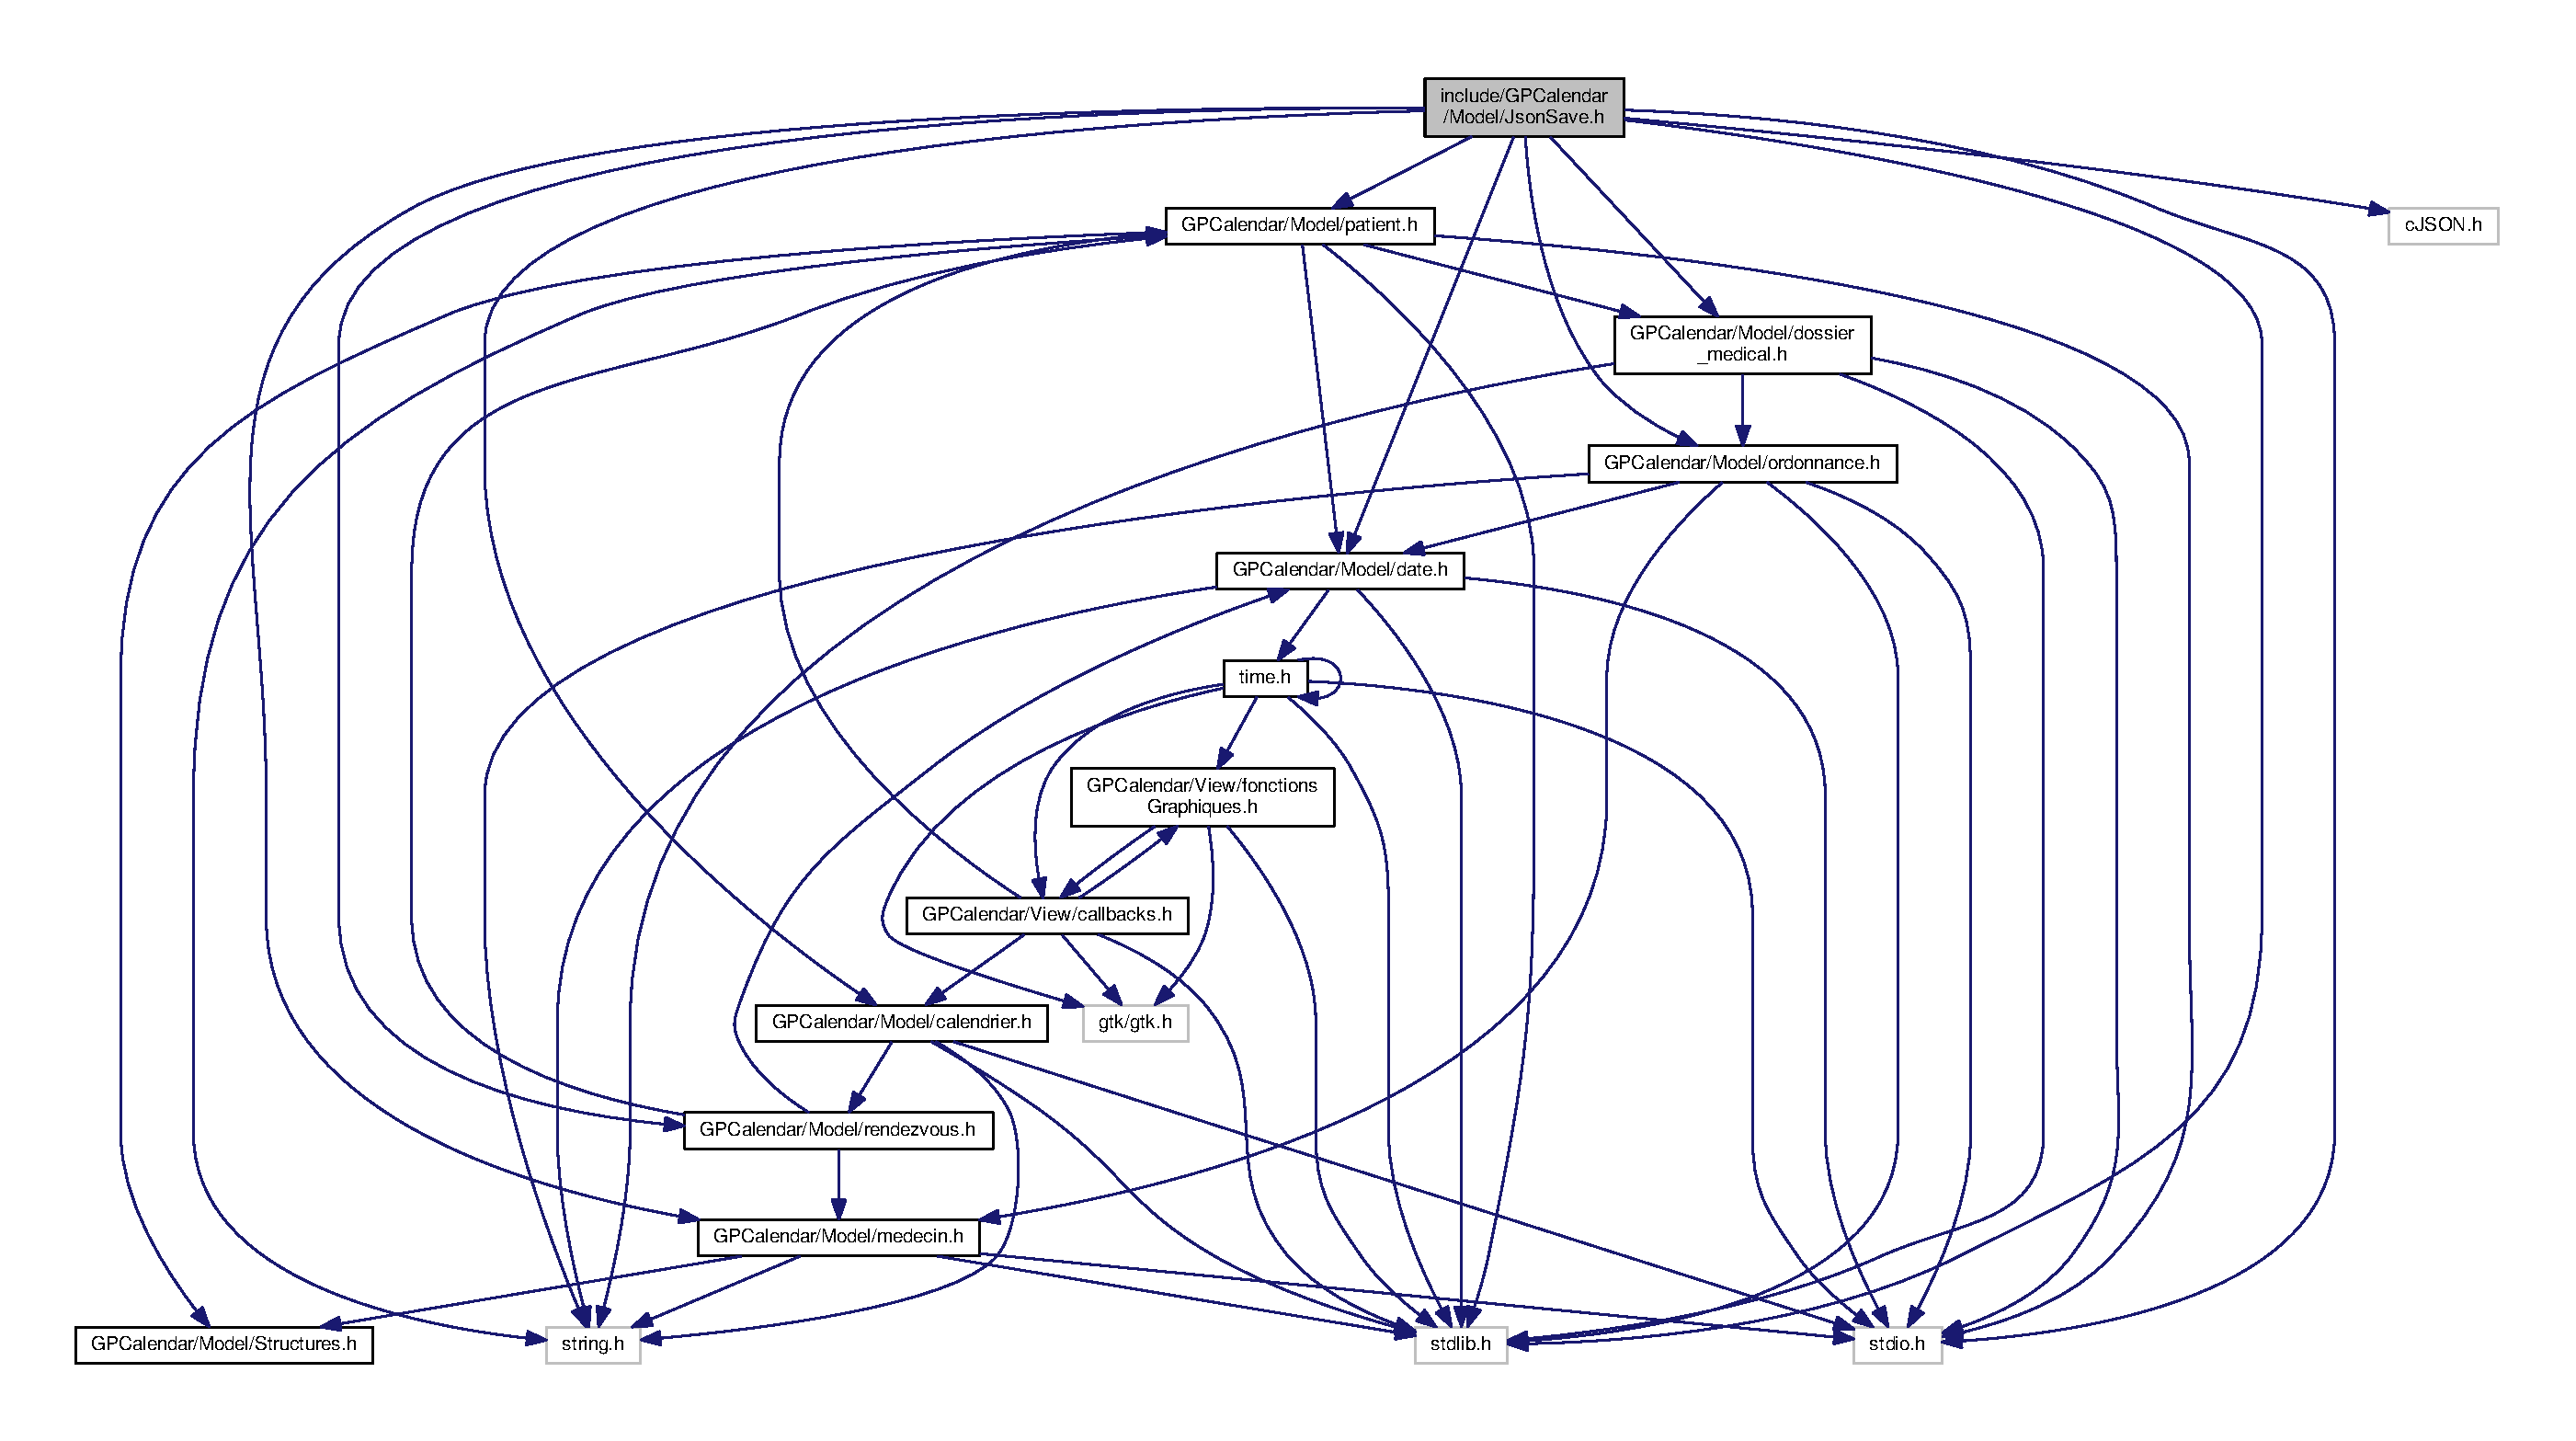
\includegraphics[width=350pt]{_json_save_8h__incl}
\end{center}
\end{figure}
Ce graphe montre quels fichiers incluent directement ou indirectement ce fichier \-:
\nopagebreak
\begin{figure}[H]
\begin{center}
\leavevmode
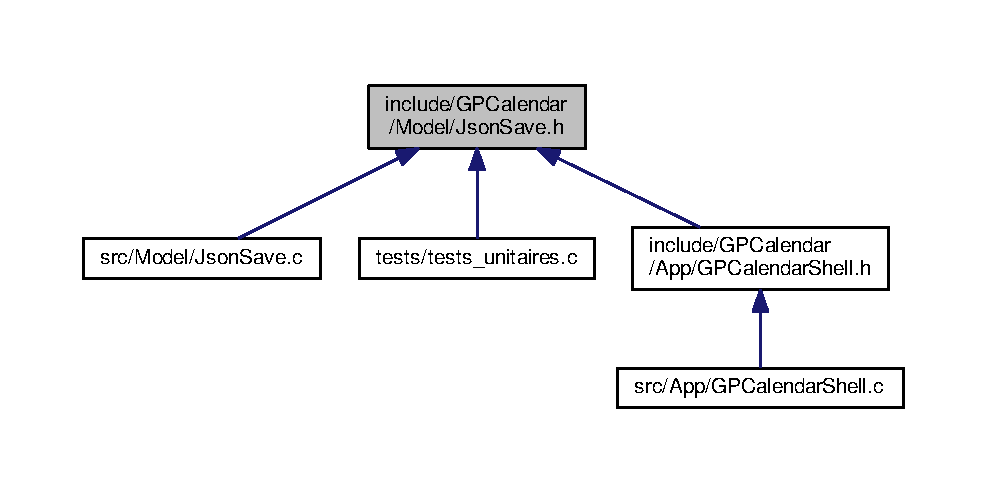
\includegraphics[width=350pt]{_json_save_8h__dep__incl}
\end{center}
\end{figure}
\subsection*{Structures de données}
\begin{DoxyCompactItemize}
\item 
struct \hyperlink{struct_project}{Project}
\end{DoxyCompactItemize}
\subsection*{Fonctions}
\begin{DoxyCompactItemize}
\item 
\hyperlink{struct_project}{Project} $\ast$ \hyperlink{_json_save_8h_a7a5fb57d9f83d9045fb81b7e6f470d38}{Creer\-Project} (char $\ast$nom, \hyperlink{struct_list_medecin}{List\-Medecin} $\ast$working\-Medecins, \hyperlink{struct_list_patient}{List\-Patient} $\ast$consulting\-Patient, \hyperlink{calendrier_8h_ab8644d1026df84be3eb3190cf1ef29fa}{Calendrier} calendrier)
\item 
void \hyperlink{_json_save_8h_aa85ffed3ee8b72ca163b8d3fef2e9c33}{free\-Project} (\hyperlink{struct_project}{Project} $\ast$project)
\item 
void \hyperlink{_json_save_8h_afe4c4f44b2d76f6636292c34aa2d261c}{print\-Project} (\hyperlink{struct_project}{Project} $\ast$p)
\item 
int \hyperlink{_json_save_8h_afd3a46e70eacecdc397b8b59c5329ed1}{G\-P\-Calendar\-\_\-save\-Project} (char $\ast$nom\-Fichier, \hyperlink{struct_project}{Project} $\ast$project)
\item 
char $\ast$ \hyperlink{_json_save_8h_aff9abd67fb976652e135b7ede413cb3f}{Project\-\_\-json\-Save} (\hyperlink{struct_project}{Project} $\ast$p)
\item 
int \hyperlink{_json_save_8h_a5c37b29882e21010d74cec620f423f85}{List\-Medecin\-\_\-json\-Save} (c\-J\-S\-O\-N $\ast$list\-Medecin\-Json, \hyperlink{struct_list_medecin}{List\-Medecin} $\ast$l)
\item 
int \hyperlink{_json_save_8h_ad49c020d48062643c39895ecc2d28e4f}{List\-Patient\-\_\-json\-Save} (c\-J\-S\-O\-N $\ast$list\-Patient\-Json, \hyperlink{struct_list_patient}{List\-Patient} $\ast$l)
\item 
int \hyperlink{_json_save_8h_a21e1346bc98e5298a55c6ea50e3c94b5}{Calendrier\-\_\-json\-Save} (c\-J\-S\-O\-N $\ast$calendrier\-Json, \hyperlink{calendrier_8h_ab8644d1026df84be3eb3190cf1ef29fa}{Calendrier} c)
\item 
\hyperlink{struct_project}{Project} $\ast$ \hyperlink{_json_save_8h_ac99dc1f99b61430d18c89660bfbdf961}{G\-P\-Calendar\-\_\-load\-Project} (char $\ast$nom\-Fichier)
\item 
\hyperlink{struct_project}{Project} $\ast$ \hyperlink{_json_save_8h_a591123cc4af0fc7f0b673fc3c73350e8}{Project\-\_\-json\-Load} (const char $\ast$content)
\item 
int \hyperlink{_json_save_8h_a7ac94075c9d7b1d6573cec905d025176}{List\-Medecin\-\_\-json\-Load} (c\-J\-S\-O\-N $\ast$project\-Json, \hyperlink{struct_list_medecin}{List\-Medecin} $\ast$l\-M)
\item 
int \hyperlink{_json_save_8h_a3bea4ff78d8287423643ba3e76f155cd}{List\-Patient\-\_\-json\-Load} (c\-J\-S\-O\-N $\ast$project\-Json, \hyperlink{struct_list_medecin}{List\-Medecin} $\ast$project\-\_\-working\-Medecins, \hyperlink{struct_list_patient}{List\-Patient} $\ast$l\-P)
\item 
int \hyperlink{_json_save_8h_a43e66b4e9f5568407bddd301964a9467}{Calendrier\-\_\-json\-Load} (c\-J\-S\-O\-N $\ast$project\-Json, \hyperlink{struct_list_medecin}{List\-Medecin} $\ast$l\-M, \hyperlink{struct_list_patient}{List\-Patient} $\ast$l\-P, \hyperlink{calendrier_8h_ab8644d1026df84be3eb3190cf1ef29fa}{Calendrier} c)
\end{DoxyCompactItemize}


\subsection{Documentation des fonctions}
\hypertarget{_json_save_8h_a43e66b4e9f5568407bddd301964a9467}{\index{Json\-Save.\-h@{Json\-Save.\-h}!Calendrier\-\_\-json\-Load@{Calendrier\-\_\-json\-Load}}
\index{Calendrier\-\_\-json\-Load@{Calendrier\-\_\-json\-Load}!JsonSave.h@{Json\-Save.\-h}}
\subsubsection[{Calendrier\-\_\-json\-Load}]{\setlength{\rightskip}{0pt plus 5cm}int Calendrier\-\_\-json\-Load (
\begin{DoxyParamCaption}
\item[{c\-J\-S\-O\-N $\ast$}]{project\-Json, }
\item[{{\bf List\-Medecin} $\ast$}]{l\-M, }
\item[{{\bf List\-Patient} $\ast$}]{l\-P, }
\item[{{\bf Calendrier}}]{c}
\end{DoxyParamCaption}
)}}\label{_json_save_8h_a43e66b4e9f5568407bddd301964a9467}
\hypertarget{_json_save_8h_a21e1346bc98e5298a55c6ea50e3c94b5}{\index{Json\-Save.\-h@{Json\-Save.\-h}!Calendrier\-\_\-json\-Save@{Calendrier\-\_\-json\-Save}}
\index{Calendrier\-\_\-json\-Save@{Calendrier\-\_\-json\-Save}!JsonSave.h@{Json\-Save.\-h}}
\subsubsection[{Calendrier\-\_\-json\-Save}]{\setlength{\rightskip}{0pt plus 5cm}int Calendrier\-\_\-json\-Save (
\begin{DoxyParamCaption}
\item[{c\-J\-S\-O\-N $\ast$}]{calendrier\-Json, }
\item[{{\bf Calendrier}}]{c}
\end{DoxyParamCaption}
)}}\label{_json_save_8h_a21e1346bc98e5298a55c6ea50e3c94b5}
Calendrier\-\_\-json\-Save \-: fonction qui écrit dans un objet c\-Json une liste de Rendez-\/vous (triée chronologiquement) 
\begin{DoxyParams}{Paramètres}
{\em calendrier\-Json} & \-: l'objet c\-J\-S\-O\-N dans lequel on sauvegarde le calendrier \\
\hline
{\em c} & \-: le calendrier à save \\
\hline
\end{DoxyParams}
\begin{DoxyReturn}{Renvoie}
1 si tout s'est bien passé 0 sinon 
\end{DoxyReturn}
Avec les 4 boucles for qui suivent on vient chercher tous les rdv\hypertarget{_json_save_8h_a7a5fb57d9f83d9045fb81b7e6f470d38}{\index{Json\-Save.\-h@{Json\-Save.\-h}!Creer\-Project@{Creer\-Project}}
\index{Creer\-Project@{Creer\-Project}!JsonSave.h@{Json\-Save.\-h}}
\subsubsection[{Creer\-Project}]{\setlength{\rightskip}{0pt plus 5cm}{\bf Project}$\ast$ Creer\-Project (
\begin{DoxyParamCaption}
\item[{char $\ast$}]{nom, }
\item[{{\bf List\-Medecin} $\ast$}]{working\-Medecins, }
\item[{{\bf List\-Patient} $\ast$}]{consulting\-Patient, }
\item[{{\bf Calendrier}}]{calendrier}
\end{DoxyParamCaption}
)}}\label{_json_save_8h_a7a5fb57d9f83d9045fb81b7e6f470d38}
\hypertarget{_json_save_8h_aa85ffed3ee8b72ca163b8d3fef2e9c33}{\index{Json\-Save.\-h@{Json\-Save.\-h}!free\-Project@{free\-Project}}
\index{free\-Project@{free\-Project}!JsonSave.h@{Json\-Save.\-h}}
\subsubsection[{free\-Project}]{\setlength{\rightskip}{0pt plus 5cm}void free\-Project (
\begin{DoxyParamCaption}
\item[{{\bf Project} $\ast$}]{project}
\end{DoxyParamCaption}
)}}\label{_json_save_8h_aa85ffed3ee8b72ca163b8d3fef2e9c33}
free\-Project \-: Free entièrement un projet, à savoir \-:
\begin{DoxyItemize}
\item le calendrier de l'hopital (et donc tous les rdv qui le composent)
\item les médecins de l'hopital qui ont été rentrés dans la liste working\-Medecins
\item les patients de l'hopital qui ont été rentrés dans la liste consulting\-Patients et donc leur dossier médical et leurs ordonnances 
\begin{DoxyParams}{Paramètres}
{\em project} & \-: le projet à free \\
\hline
\end{DoxyParams}

\end{DoxyItemize}\hypertarget{_json_save_8h_ac99dc1f99b61430d18c89660bfbdf961}{\index{Json\-Save.\-h@{Json\-Save.\-h}!G\-P\-Calendar\-\_\-load\-Project@{G\-P\-Calendar\-\_\-load\-Project}}
\index{G\-P\-Calendar\-\_\-load\-Project@{G\-P\-Calendar\-\_\-load\-Project}!JsonSave.h@{Json\-Save.\-h}}
\subsubsection[{G\-P\-Calendar\-\_\-load\-Project}]{\setlength{\rightskip}{0pt plus 5cm}{\bf Project}$\ast$ G\-P\-Calendar\-\_\-load\-Project (
\begin{DoxyParamCaption}
\item[{char $\ast$}]{nom\-Fichier}
\end{DoxyParamCaption}
)}}\label{_json_save_8h_ac99dc1f99b61430d18c89660bfbdf961}
G\-P\-Calendar\-\_\-load\-Project \-: fonction récupérant les données d'un projet depuis un fichier au format J\-S\-O\-N 
\begin{DoxyParams}{Paramètres}
{\em nom\-Fichier} & \-: le fichier depuis lequel on récupère les données \\
\hline
\end{DoxyParams}
\begin{DoxyReturn}{Renvoie}
un pointeur sur le projet créé avec les données J\-S\-O\-N 
\end{DoxyReturn}
\hypertarget{_json_save_8h_afd3a46e70eacecdc397b8b59c5329ed1}{\index{Json\-Save.\-h@{Json\-Save.\-h}!G\-P\-Calendar\-\_\-save\-Project@{G\-P\-Calendar\-\_\-save\-Project}}
\index{G\-P\-Calendar\-\_\-save\-Project@{G\-P\-Calendar\-\_\-save\-Project}!JsonSave.h@{Json\-Save.\-h}}
\subsubsection[{G\-P\-Calendar\-\_\-save\-Project}]{\setlength{\rightskip}{0pt plus 5cm}int G\-P\-Calendar\-\_\-save\-Project (
\begin{DoxyParamCaption}
\item[{char $\ast$}]{nom\-Fichier, }
\item[{{\bf Project} $\ast$}]{project}
\end{DoxyParamCaption}
)}}\label{_json_save_8h_afd3a46e70eacecdc397b8b59c5329ed1}
Pour l'instant On ne sauvegarde pas les diplomes et spécialités des médecins ainsi que les antécédents des Dossier\-Médicaux G\-P\-Calendar\-\_\-save\-Project \-: Sauvegarde un projet (liste de médecins, patients et un calendrier) sous forme de fichier texte au format J\-S\-O\-N 
\begin{DoxyParams}{Paramètres}
{\em nom\-Fichier} & \-: le nom du fichier qui contiendra les données au format J\-S\-O\-N \\
\hline
{\em project} & \-: le projet à sauvegarder \\
\hline
\end{DoxyParams}
\begin{DoxyReturn}{Renvoie}
1 si tout s'est bien passé 0 sinon (erreur d'ouverture de fichier ou de parsing \-: Cf c\-J\-S\-O\-N) 
\end{DoxyReturn}
\hypertarget{_json_save_8h_a7ac94075c9d7b1d6573cec905d025176}{\index{Json\-Save.\-h@{Json\-Save.\-h}!List\-Medecin\-\_\-json\-Load@{List\-Medecin\-\_\-json\-Load}}
\index{List\-Medecin\-\_\-json\-Load@{List\-Medecin\-\_\-json\-Load}!JsonSave.h@{Json\-Save.\-h}}
\subsubsection[{List\-Medecin\-\_\-json\-Load}]{\setlength{\rightskip}{0pt plus 5cm}int List\-Medecin\-\_\-json\-Load (
\begin{DoxyParamCaption}
\item[{c\-J\-S\-O\-N $\ast$}]{project\-Json, }
\item[{{\bf List\-Medecin} $\ast$}]{l\-M}
\end{DoxyParamCaption}
)}}\label{_json_save_8h_a7ac94075c9d7b1d6573cec905d025176}
List\-Medecin\-\_\-json\-Load \-: Load depuis un objet c\-J\-S\-O\-N une liste de médecins 
\begin{DoxyParams}{Paramètres}
{\em project\-Json} & \-: l'objet c\-J\-S\-O\-N contenant les données pour la liste de médecins \\
\hline
\end{DoxyParams}
\begin{DoxyReturn}{Renvoie}
1 si tout s'est bien passé 0 sinon 
\end{DoxyReturn}
\hypertarget{_json_save_8h_a5c37b29882e21010d74cec620f423f85}{\index{Json\-Save.\-h@{Json\-Save.\-h}!List\-Medecin\-\_\-json\-Save@{List\-Medecin\-\_\-json\-Save}}
\index{List\-Medecin\-\_\-json\-Save@{List\-Medecin\-\_\-json\-Save}!JsonSave.h@{Json\-Save.\-h}}
\subsubsection[{List\-Medecin\-\_\-json\-Save}]{\setlength{\rightskip}{0pt plus 5cm}int List\-Medecin\-\_\-json\-Save (
\begin{DoxyParamCaption}
\item[{c\-J\-S\-O\-N $\ast$}]{list\-Medecin\-Json, }
\item[{{\bf List\-Medecin} $\ast$}]{l}
\end{DoxyParamCaption}
)}}\label{_json_save_8h_a5c37b29882e21010d74cec620f423f85}
List\-Medecin\-\_\-json\-Save \-: fonction qui écrit dans un objet c\-Json une liste de médecins Chaque médecin possédant une liste de patients recus, on écrira uniquement l'I\-D de ces patients (= leur numéro de sécurité social) dans cette liste 
\begin{DoxyParams}{Paramètres}
{\em list\-Medecin\-Json} & \-: l'objet c\-Json dans lequel on écrit la liste de médecins, c'est un tableau \\
\hline
{\em l} & \-: la liste de médecins à écrire \\
\hline
\end{DoxyParams}
\begin{DoxyReturn}{Renvoie}
1 si tout s'est bien passé 0 si une des étapes a échoué 
\end{DoxyReturn}
On gère la liste des patients recus \-: on crée un tableau, on parcourt la liste des patients recus et à chaque patient on crée un string avec son numéro de sécurité sociale puis on ajoute ce string au tableau que l'on vient de créer et à la fin du parcours de la liste on ajoute notre tableau à son médecin

E\-D\-I\-T \-: P\-O\-U\-R L\-A V0 O\-N N\-E M\-E\-T P\-A\-S L\-E\-S P\-A\-T\-I\-E\-N\-T\-S R\-E\-C\-U\-S \-: T\-R\-O\-P G\-A\-L\-E\-R\-E, O\-N A\-J\-O\-U\-T\-E\-R\-A L\-E\-S C\-O\-U\-P\-L\-E\-S P\-A\-T\-I\-E\-N\-T / M\-E\-D\-E\-C\-I\-N D\-E\-P\-U\-I\-S L\-E\-S R\-D\-V\hypertarget{_json_save_8h_a3bea4ff78d8287423643ba3e76f155cd}{\index{Json\-Save.\-h@{Json\-Save.\-h}!List\-Patient\-\_\-json\-Load@{List\-Patient\-\_\-json\-Load}}
\index{List\-Patient\-\_\-json\-Load@{List\-Patient\-\_\-json\-Load}!JsonSave.h@{Json\-Save.\-h}}
\subsubsection[{List\-Patient\-\_\-json\-Load}]{\setlength{\rightskip}{0pt plus 5cm}int List\-Patient\-\_\-json\-Load (
\begin{DoxyParamCaption}
\item[{c\-J\-S\-O\-N $\ast$}]{project\-Json, }
\item[{{\bf List\-Medecin} $\ast$}]{project\-\_\-working\-Medecins, }
\item[{{\bf List\-Patient} $\ast$}]{l\-P}
\end{DoxyParamCaption}
)}}\label{_json_save_8h_a3bea4ff78d8287423643ba3e76f155cd}
\hypertarget{_json_save_8h_ad49c020d48062643c39895ecc2d28e4f}{\index{Json\-Save.\-h@{Json\-Save.\-h}!List\-Patient\-\_\-json\-Save@{List\-Patient\-\_\-json\-Save}}
\index{List\-Patient\-\_\-json\-Save@{List\-Patient\-\_\-json\-Save}!JsonSave.h@{Json\-Save.\-h}}
\subsubsection[{List\-Patient\-\_\-json\-Save}]{\setlength{\rightskip}{0pt plus 5cm}int List\-Patient\-\_\-json\-Save (
\begin{DoxyParamCaption}
\item[{c\-J\-S\-O\-N $\ast$}]{list\-Patient\-Json, }
\item[{{\bf List\-Patient} $\ast$}]{l}
\end{DoxyParamCaption}
)}}\label{_json_save_8h_ad49c020d48062643c39895ecc2d28e4f}
List\-Patient\-\_\-json\-Save \-: fonction qui écrit dans un objet c\-Json une liste de patient Chaque patient possédant un dossier médical possédant lui même une liste de medecins consultes et une liste d'ordonnances On écrira directement ces infos dans le patient (pour éviter la création d'une liste de dossier médicaux inutile) Et on écrira uniquement l'I\-D des medecins consultes (= leur numéro R\-P\-S) dans cette liste de medecin dans patient Puis un tableau d'ordonnances représentant la liste des ordonnaces du dossier médical du patient 
\begin{DoxyParams}{Paramètres}
{\em list\-Patient\-Json} & \-: l'objet c\-Json dans lequel on écrit la liste de patient, c'est un tableau \\
\hline
{\em l} & \-: la liste de patients à save \\
\hline
\end{DoxyParams}
\begin{DoxyReturn}{Renvoie}
1 si tout s'est bien passé 0 si une des étapes a échoué 
\end{DoxyReturn}
On gère la liste des medecins consultes \-: on crée un tableau, on parcourt la liste des medecins consultes et à chaque medecin on crée un string avec son numéro\-\_\-\-R\-P\-S puis on ajoute ce string au tableau que l'on vient de créer et à la fin du parcours de la liste on ajoute notre tableau à son patient

E\-D\-I\-T \-: P\-O\-U\-R L\-A V0 O\-N N\-E M\-E\-T P\-A\-S L\-E\-S M\-E\-D\-E\-C\-I\-N\-S C\-O\-N\-S\-U\-L\-T\-E\-S \-: T\-R\-O\-P G\-A\-L\-E\-R\-E, O\-N A\-J\-O\-U\-T\-E\-R\-A L\-E\-S C\-O\-U\-P\-L\-E\-S P\-A\-T\-I\-E\-N\-T / M\-E\-D\-E\-C\-I\-N D\-E\-P\-U\-I\-S L\-E\-S R\-D\-V

On gère la liste d'ordonnances du dossier médical de notre patient\hypertarget{_json_save_8h_afe4c4f44b2d76f6636292c34aa2d261c}{\index{Json\-Save.\-h@{Json\-Save.\-h}!print\-Project@{print\-Project}}
\index{print\-Project@{print\-Project}!JsonSave.h@{Json\-Save.\-h}}
\subsubsection[{print\-Project}]{\setlength{\rightskip}{0pt plus 5cm}void print\-Project (
\begin{DoxyParamCaption}
\item[{{\bf Project} $\ast$}]{p}
\end{DoxyParamCaption}
)}}\label{_json_save_8h_afe4c4f44b2d76f6636292c34aa2d261c}
print\-Project \-: Affiche dans la console toutes les données d'un projet 
\begin{DoxyParams}{Paramètres}
{\em p} & \-: le projet à afficher \\
\hline
\end{DoxyParams}
\hypertarget{_json_save_8h_a591123cc4af0fc7f0b673fc3c73350e8}{\index{Json\-Save.\-h@{Json\-Save.\-h}!Project\-\_\-json\-Load@{Project\-\_\-json\-Load}}
\index{Project\-\_\-json\-Load@{Project\-\_\-json\-Load}!JsonSave.h@{Json\-Save.\-h}}
\subsubsection[{Project\-\_\-json\-Load}]{\setlength{\rightskip}{0pt plus 5cm}{\bf Project}$\ast$ Project\-\_\-json\-Load (
\begin{DoxyParamCaption}
\item[{const char $\ast$const}]{content}
\end{DoxyParamCaption}
)}}\label{_json_save_8h_a591123cc4af0fc7f0b673fc3c73350e8}
Project\-\_\-json\-Load \-: Crée un objet project depuis un char$\ast$ au format J\-S\-O\-N 
\begin{DoxyParams}{Paramètres}
{\em content} & \-: le char$\ast$ avec les données du projet \\
\hline
\end{DoxyParams}
\begin{DoxyReturn}{Renvoie}
un pointeur sur le projet créé si tout s'est bien passé N\-U\-L\-L si un erreur a eu lieu (Cf c\-J\-S\-O\-N) 
\end{DoxyReturn}
\hypertarget{_json_save_8h_aff9abd67fb976652e135b7ede413cb3f}{\index{Json\-Save.\-h@{Json\-Save.\-h}!Project\-\_\-json\-Save@{Project\-\_\-json\-Save}}
\index{Project\-\_\-json\-Save@{Project\-\_\-json\-Save}!JsonSave.h@{Json\-Save.\-h}}
\subsubsection[{Project\-\_\-json\-Save}]{\setlength{\rightskip}{0pt plus 5cm}char$\ast$ Project\-\_\-json\-Save (
\begin{DoxyParamCaption}
\item[{{\bf Project} $\ast$}]{project}
\end{DoxyParamCaption}
)}}\label{_json_save_8h_aff9abd67fb976652e135b7ede413cb3f}
Project\-\_\-json\-Save \-: Fonction permettant de sauvegarder un objet projet dans un fichier .json à l'aide de la librairie cjson 
\begin{DoxyParams}{Paramètres}
{\em p} & \-: l'instance de projet à save \\
\hline
\end{DoxyParams}
\begin{DoxyReturn}{Renvoie}
un string qui sera écrit dans un fichier texte 
\end{DoxyReturn}

\hypertarget{medecin_8h}{\section{Référence du fichier include/\-G\-P\-Calendar/\-Model/medecin.h}
\label{medecin_8h}\index{include/\-G\-P\-Calendar/\-Model/medecin.\-h@{include/\-G\-P\-Calendar/\-Model/medecin.\-h}}
}
{\ttfamily \#include \char`\"{}G\-P\-Calendar/\-Model/\-Structures.\-h\char`\"{}}\\*
{\ttfamily \#include $<$string.\-h$>$}\\*
{\ttfamily \#include $<$stdlib.\-h$>$}\\*
{\ttfamily \#include $<$stdio.\-h$>$}\\*
Graphe des dépendances par inclusion de medecin.\-h\-:
\nopagebreak
\begin{figure}[H]
\begin{center}
\leavevmode
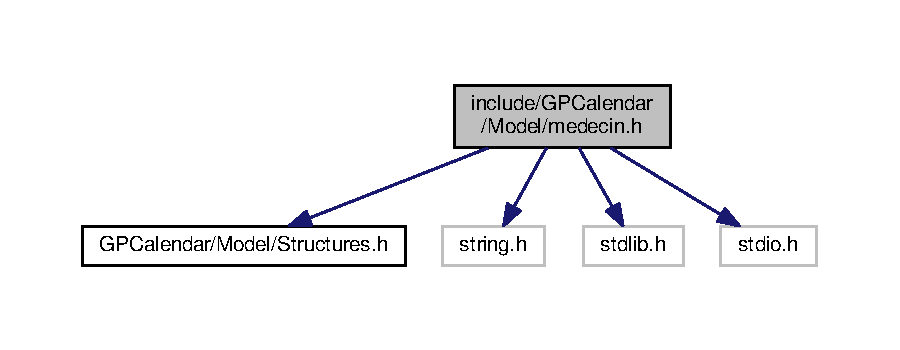
\includegraphics[width=350pt]{medecin_8h__incl}
\end{center}
\end{figure}
Ce graphe montre quels fichiers incluent directement ou indirectement ce fichier \-:
\nopagebreak
\begin{figure}[H]
\begin{center}
\leavevmode
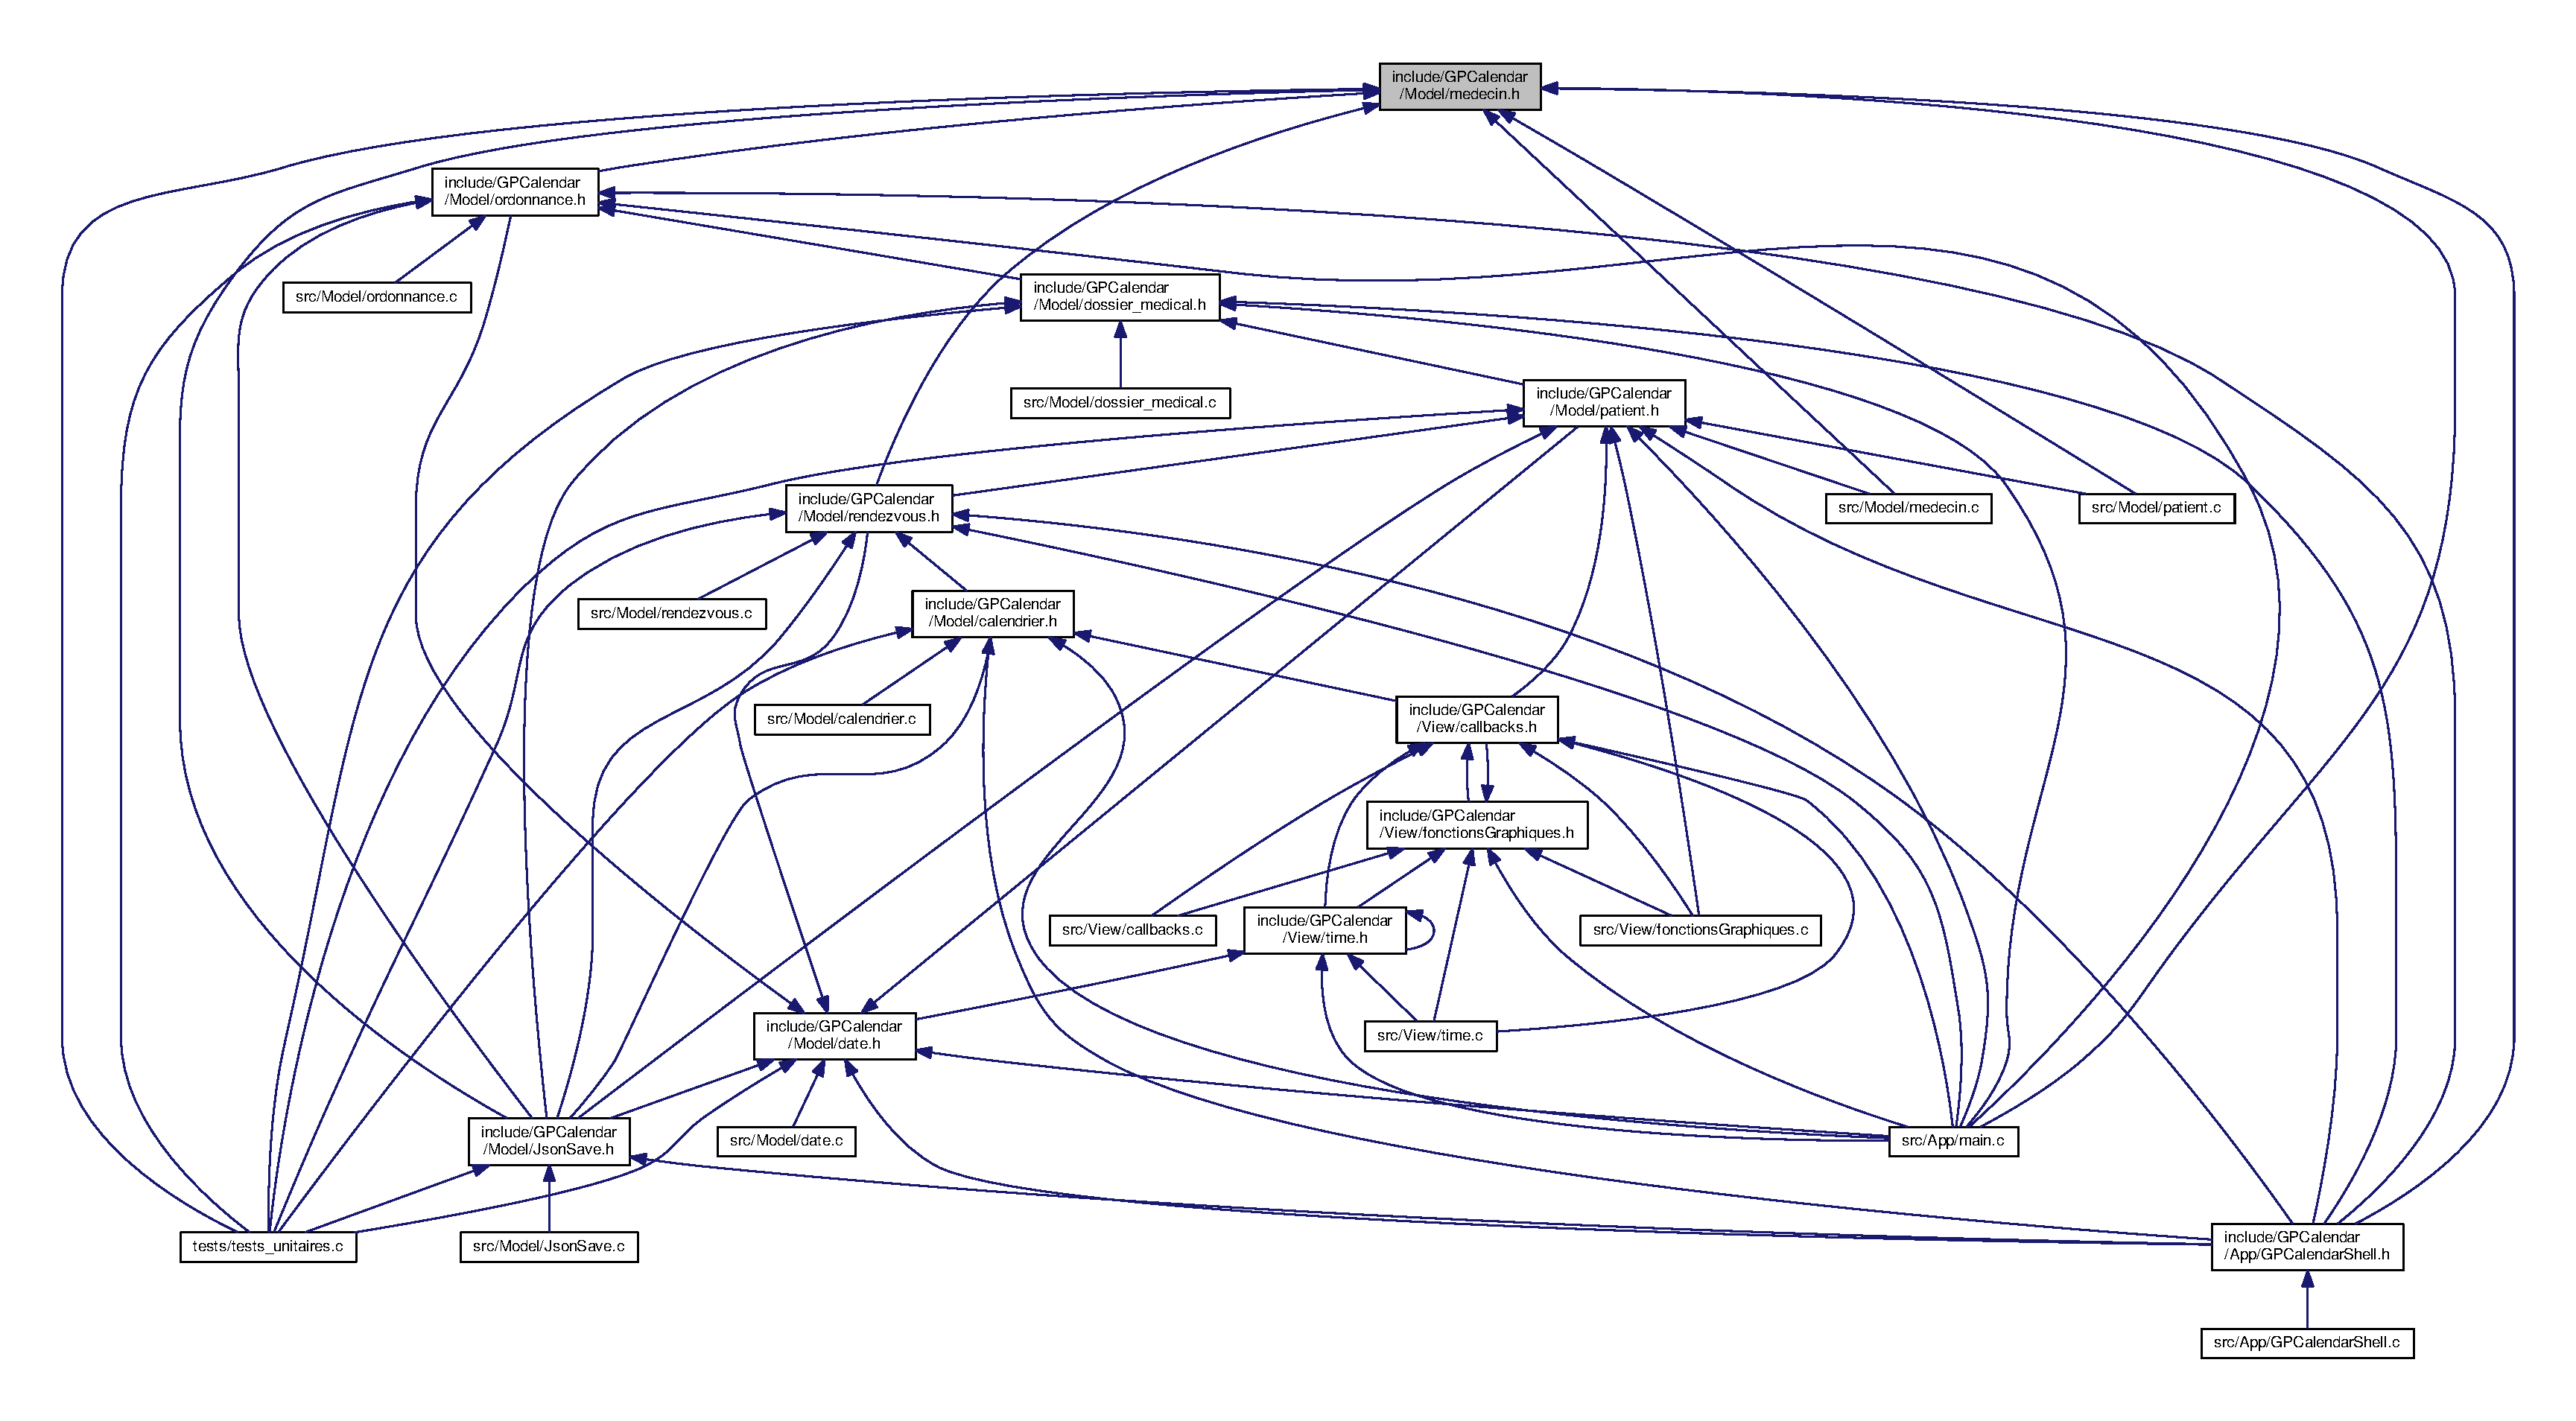
\includegraphics[width=350pt]{medecin_8h__dep__incl}
\end{center}
\end{figure}
\subsection*{Structures de données}
\begin{DoxyCompactItemize}
\item 
struct \hyperlink{struct_medecin}{Medecin}
\item 
struct \hyperlink{struct_node_medecin}{Node\-Medecin}
\item 
struct \hyperlink{struct_list_medecin}{List\-Medecin}
\end{DoxyCompactItemize}
\subsection*{Définitions de type}
\begin{DoxyCompactItemize}
\item 
typedef struct \hyperlink{struct_node_medecin}{Node\-Medecin} \hyperlink{medecin_8h_aa1ed637873e0ef67d582b0881c7640e4}{Node\-Medecin}
\end{DoxyCompactItemize}
\subsection*{Fonctions}
\begin{DoxyCompactItemize}
\item 
\hyperlink{struct_medecin}{Medecin} $\ast$ \hyperlink{medecin_8h_a0afe5fb66e0cb635d1ab76b51a6b1758}{Creer\-Medecin} (char $\ast$nom, char $\ast$prenom, char $\ast$mail, char $\ast$num\-\_\-tel, char $\ast$num\-\_\-\-R\-P\-S)
\item 
void \hyperlink{medecin_8h_a71bcd5e35819a7252983451b7a6397d8}{Delete\-Medecin} (\hyperlink{struct_medecin}{Medecin} $\ast$medecin)
\item 
void \hyperlink{medecin_8h_a05bcf828900177b22789cd327fc16c34}{Affiche\-Medecin} (\hyperlink{struct_medecin}{Medecin} $\ast$m)
\item 
void \hyperlink{medecin_8h_a351b689795ff9543c5ed4236f3934d04}{Set\-Nom\-Medecin} (\hyperlink{struct_medecin}{Medecin} $\ast$medecin, char $\ast$nom)
\item 
void \hyperlink{medecin_8h_ab0ea71bb483a62977a39b3cefc018783}{Set\-Prenom\-Medecin} (\hyperlink{struct_medecin}{Medecin} $\ast$medecin, char $\ast$prenom)
\item 
void \hyperlink{medecin_8h_a6f15cb667271234dd0f0e6433be5d060}{Set\-Adresse\-Mail\-Medecin} (\hyperlink{struct_medecin}{Medecin} $\ast$medecin, char $\ast$mail)
\item 
void \hyperlink{medecin_8h_aa1bcc618408c8c672056f01110a4f41d}{Set\-Numero\-Telephone\-Medecin} (\hyperlink{struct_medecin}{Medecin} $\ast$medecin, char $\ast$tel)
\item 
void \hyperlink{medecin_8h_a9176e649f75181c288b50f1abae82759}{Set\-Numero\-R\-P\-S\-Medecin} (\hyperlink{struct_medecin}{Medecin} $\ast$medecin, char $\ast$num\-\_\-\-R\-P\-S)
\item 
void \hyperlink{medecin_8h_a59bd5d29002e8d49f09775294999b57f}{get\-Nom\-Medecin} (char $\ast$nom, \hyperlink{struct_medecin}{Medecin} $\ast$m)
\item 
char $\ast$ \hyperlink{medecin_8h_a4e4bf2ef1e173182f36ff76165acb777}{get\-Adresse\-Mail\-Medecin} (\hyperlink{struct_medecin}{Medecin} $\ast$medecin)
\item 
char $\ast$ \hyperlink{medecin_8h_a930b0a763fdcfec514809669fbbd5290}{get\-Numero\-Telephone\-Medecin} (\hyperlink{struct_medecin}{Medecin} $\ast$medecin)
\item 
char $\ast$ \hyperlink{medecin_8h_a1bd4693b2cb4795a4b749866e9127a09}{get\-Numero\-R\-P\-S\-Medecin} (\hyperlink{struct_medecin}{Medecin} $\ast$medecin)
\item 
void \hyperlink{medecin_8h_a6e47cda987182a19e519a89782bc63f1}{get\-Info\-Medecin} (char $\ast$infos, \hyperlink{struct_medecin}{Medecin} $\ast$medecin)
\item 
int \hyperlink{medecin_8h_a318de0429082e499ecfa239ea25c2a95}{Init\-Patient\-Recus\-Medecin} (\hyperlink{struct_medecin}{Medecin} $\ast$medecin)
\item 
void \hyperlink{medecin_8h_a69f13e90460e67c36a8a9a1d2fed8920}{Free\-Patient\-Recus\-Medecin} (\hyperlink{struct_medecin}{Medecin} $\ast$medecin)
\item 
int \hyperlink{medecin_8h_ae523afbd8be2ec7cbf04c5990e22e5f6}{Add\-Patient\-Recu\-Medecin} (\hyperlink{struct_medecin}{Medecin} $\ast$m, \hyperlink{struct_patient}{Patient} $\ast$patient)
\item 
int \hyperlink{medecin_8h_aa1ee02a57bad305bda1ac2510370e3c0}{Delete\-Patient\-Recu\-Medecin} (\hyperlink{struct_medecin}{Medecin} $\ast$m, \hyperlink{struct_patient}{Patient} $\ast$patient)
\item 
\hyperlink{struct_node_medecin}{Node\-Medecin} $\ast$ \hyperlink{medecin_8h_ae44be774cac54154a80da40db3bcc6a6}{new\-Node\-Medecin} (\hyperlink{struct_medecin}{Medecin} $\ast$medecin, \hyperlink{struct_node_medecin}{Node\-Medecin} $\ast$previous, \hyperlink{struct_node_medecin}{Node\-Medecin} $\ast$next)
\item 
void \hyperlink{medecin_8h_a96995b3a980662761de97d6024d9ecf4}{free\-Node\-Medecin} (\hyperlink{struct_list_medecin}{List\-Medecin} $\ast$l, \hyperlink{struct_node_medecin}{Node\-Medecin} $\ast$n)
\item 
void \hyperlink{medecin_8h_a7d0ca07d61f1aab69e37294af0a2a924}{free\-Node\-Medecin\-\_\-without\-Deleting\-Medecin} (\hyperlink{struct_list_medecin}{List\-Medecin} $\ast$l, \hyperlink{struct_node_medecin}{Node\-Medecin} $\ast$n)
\item 
\hyperlink{struct_list_medecin}{List\-Medecin} $\ast$ \hyperlink{medecin_8h_ae1cfbfa2117c0a7b5a7218017f2a7f75}{Creer\-List\-Medecin} ()
\item 
void \hyperlink{medecin_8h_acac056ba7705fe9857a63dc2df920e0d}{print\-List\-Medecin} (\hyperlink{struct_list_medecin}{List\-Medecin} $\ast$l)
\item 
void \hyperlink{medecin_8h_abf8a93013bb8621ea73405a9b741a26d}{List\-Medecin\-\_\-init} (\hyperlink{struct_list_medecin}{List\-Medecin} $\ast$l)
\item 
void \hyperlink{medecin_8h_af77a41e56d333dfe3cac87dc4207dc1c}{List\-Medecin\-\_\-free} (\hyperlink{struct_list_medecin}{List\-Medecin} $\ast$l)
\item 
void \hyperlink{medecin_8h_a33d35f3a662b16d86c05261b44a32e98}{List\-Medecin\-\_\-free\-\_\-without\-Deleting\-Medecin} (\hyperlink{struct_list_medecin}{List\-Medecin} $\ast$l)
\item 
int \hyperlink{medecin_8h_ab3522c7b9f20aa7fcecc4392251d1a0c}{List\-Medecin\-\_\-add} (\hyperlink{struct_list_medecin}{List\-Medecin} $\ast$l, \hyperlink{struct_medecin}{Medecin} $\ast$m)
\item 
\hyperlink{struct_medecin}{Medecin} $\ast$ \hyperlink{medecin_8h_acdf3f272f044ddfcc66e2d0118ae89b5}{List\-Medecin\-\_\-seek} (\hyperlink{struct_list_medecin}{List\-Medecin} $\ast$l\-P, char $\ast$I\-D\-Medecin)
\item 
int \hyperlink{medecin_8h_a7b1b4efabf71bc3ee7195ad73f953189}{List\-Medecin\-\_\-is\-Empty} (\hyperlink{struct_list_medecin}{List\-Medecin} $\ast$l)
\item 
int \hyperlink{medecin_8h_a3ad08529d7153844dfdb4121e95cfcd9}{List\-Medecin\-\_\-is\-First} (\hyperlink{struct_list_medecin}{List\-Medecin} $\ast$l)
\item 
int \hyperlink{medecin_8h_a54b718985c956faf4a6b917c55c3b934}{List\-Medecin\-\_\-is\-Last} (\hyperlink{struct_list_medecin}{List\-Medecin} $\ast$l)
\item 
int \hyperlink{medecin_8h_a6b57e943628fac1c5739ac370f06d983}{List\-Medecin\-\_\-is\-Out\-Of\-List} (\hyperlink{struct_list_medecin}{List\-Medecin} $\ast$l)
\item 
void \hyperlink{medecin_8h_ae1511c4a3885355a88a6b87040298168}{List\-Medecin\-\_\-set\-On\-First} (\hyperlink{struct_list_medecin}{List\-Medecin} $\ast$l)
\item 
void \hyperlink{medecin_8h_a6a33d1d7aeec168b9db04680114bbb2d}{List\-Medecin\-\_\-set\-On\-Last} (\hyperlink{struct_list_medecin}{List\-Medecin} $\ast$l)
\item 
void \hyperlink{medecin_8h_af977ed01cae64e1d77011a3c6555d88e}{List\-Medecin\-\_\-set\-On\-Next} (\hyperlink{struct_list_medecin}{List\-Medecin} $\ast$l)
\item 
void \hyperlink{medecin_8h_a7e65abd3210688fdb92699ef2e2ade15}{List\-Medecin\-\_\-set\-On\-Previous} (\hyperlink{struct_list_medecin}{List\-Medecin} $\ast$l)
\item 
\hyperlink{struct_medecin}{Medecin} $\ast$ \hyperlink{medecin_8h_a97a3982adfbf8b1deb4abdb091dee173}{List\-Medecin\-\_\-get\-Current} (\hyperlink{struct_list_medecin}{List\-Medecin} $\ast$l)
\end{DoxyCompactItemize}


\subsection{Documentation des définitions de type}
\hypertarget{medecin_8h_aa1ed637873e0ef67d582b0881c7640e4}{\index{medecin.\-h@{medecin.\-h}!Node\-Medecin@{Node\-Medecin}}
\index{Node\-Medecin@{Node\-Medecin}!medecin.h@{medecin.\-h}}
\subsubsection[{Node\-Medecin}]{\setlength{\rightskip}{0pt plus 5cm}typedef struct {\bf Node\-Medecin} {\bf Node\-Medecin}}}\label{medecin_8h_aa1ed637873e0ef67d582b0881c7640e4}
Structure \hyperlink{struct_node_medecin}{Node\-Medecin} permettant de créer une Doubly linked list pour la liste des medecins consultés par un patient 

\subsection{Documentation des fonctions}
\hypertarget{medecin_8h_ae523afbd8be2ec7cbf04c5990e22e5f6}{\index{medecin.\-h@{medecin.\-h}!Add\-Patient\-Recu\-Medecin@{Add\-Patient\-Recu\-Medecin}}
\index{Add\-Patient\-Recu\-Medecin@{Add\-Patient\-Recu\-Medecin}!medecin.h@{medecin.\-h}}
\subsubsection[{Add\-Patient\-Recu\-Medecin}]{\setlength{\rightskip}{0pt plus 5cm}int Add\-Patient\-Recu\-Medecin (
\begin{DoxyParamCaption}
\item[{{\bf Medecin} $\ast$}]{m, }
\item[{{\bf Patient} $\ast$}]{patient}
\end{DoxyParamCaption}
)}}\label{medecin_8h_ae523afbd8be2ec7cbf04c5990e22e5f6}
Add\-Patient\-Recu\-Medecin \-: Ajoute un patient à la liste des patient recus par un medecin 
\begin{DoxyParams}{Paramètres}
{\em m} & \-: le medecin recevant \\
\hline
{\em patient} & \-: le patient recu \\
\hline
\end{DoxyParams}
\begin{DoxyReturn}{Renvoie}
1 si le patient a bien été ajouté à la liste 0 sinon (patient déjà recu par exemple) 
\end{DoxyReturn}
\hypertarget{medecin_8h_a05bcf828900177b22789cd327fc16c34}{\index{medecin.\-h@{medecin.\-h}!Affiche\-Medecin@{Affiche\-Medecin}}
\index{Affiche\-Medecin@{Affiche\-Medecin}!medecin.h@{medecin.\-h}}
\subsubsection[{Affiche\-Medecin}]{\setlength{\rightskip}{0pt plus 5cm}void Affiche\-Medecin (
\begin{DoxyParamCaption}
\item[{{\bf Medecin} $\ast$}]{m}
\end{DoxyParamCaption}
)}}\label{medecin_8h_a05bcf828900177b22789cd327fc16c34}
Affiche\-Medecin \-: Affiche les informations d'un medecin dans la console 
\begin{DoxyParams}{Paramètres}
{\em m} & \-: le medecin \\
\hline
\end{DoxyParams}
\hypertarget{medecin_8h_ae1cfbfa2117c0a7b5a7218017f2a7f75}{\index{medecin.\-h@{medecin.\-h}!Creer\-List\-Medecin@{Creer\-List\-Medecin}}
\index{Creer\-List\-Medecin@{Creer\-List\-Medecin}!medecin.h@{medecin.\-h}}
\subsubsection[{Creer\-List\-Medecin}]{\setlength{\rightskip}{0pt plus 5cm}{\bf List\-Medecin}$\ast$ Creer\-List\-Medecin (
\begin{DoxyParamCaption}
{}
\end{DoxyParamCaption}
)}}\label{medecin_8h_ae1cfbfa2117c0a7b5a7218017f2a7f75}
Creer\-List\-Medecin \-: malloc et initialise une liste de médecins \begin{DoxyReturn}{Renvoie}
la liste initialisée 
\end{DoxyReturn}
\hypertarget{medecin_8h_a0afe5fb66e0cb635d1ab76b51a6b1758}{\index{medecin.\-h@{medecin.\-h}!Creer\-Medecin@{Creer\-Medecin}}
\index{Creer\-Medecin@{Creer\-Medecin}!medecin.h@{medecin.\-h}}
\subsubsection[{Creer\-Medecin}]{\setlength{\rightskip}{0pt plus 5cm}{\bf Medecin}$\ast$ Creer\-Medecin (
\begin{DoxyParamCaption}
\item[{char $\ast$}]{nom, }
\item[{char $\ast$}]{prenom, }
\item[{char $\ast$}]{mail, }
\item[{char $\ast$}]{num\-\_\-tel, }
\item[{char $\ast$}]{num\-\_\-\-R\-P\-S}
\end{DoxyParamCaption}
)}}\label{medecin_8h_a0afe5fb66e0cb635d1ab76b51a6b1758}
Creer\-Medecin \-: Creer une nouvelle instance de la structure \hyperlink{struct_medecin}{Medecin} avec toutes les informations basiques mais pas ses spécialités ou ses diplômes 
\begin{DoxyParams}{Paramètres}
{\em nom} & \-: le nom du medecin \\
\hline
{\em prenom} & \-: le prenom du medecin \\
\hline
{\em mail} & \-: l'adresse mail du medecin \\
\hline
{\em num\-\_\-tel} & \-: le numero de telephone du medecin \\
\hline
{\em num\-\_\-\-R\-P\-S} & \-: le numéro R\-P\-S du medecin \\
\hline
\end{DoxyParams}
\begin{DoxyReturn}{Renvoie}
un pointeur sur le medecin créé 
\end{DoxyReturn}
\hypertarget{medecin_8h_a71bcd5e35819a7252983451b7a6397d8}{\index{medecin.\-h@{medecin.\-h}!Delete\-Medecin@{Delete\-Medecin}}
\index{Delete\-Medecin@{Delete\-Medecin}!medecin.h@{medecin.\-h}}
\subsubsection[{Delete\-Medecin}]{\setlength{\rightskip}{0pt plus 5cm}void Delete\-Medecin (
\begin{DoxyParamCaption}
\item[{{\bf Medecin} $\ast$}]{medecin}
\end{DoxyParamCaption}
)}}\label{medecin_8h_a71bcd5e35819a7252983451b7a6397d8}
Delete\-Medecin \-: Supprime proprement une instance de la structure medecin 
\begin{DoxyParams}{Paramètres}
{\em medecin} & \-: le medecin à supprimer \\
\hline
\end{DoxyParams}
\hypertarget{medecin_8h_aa1ee02a57bad305bda1ac2510370e3c0}{\index{medecin.\-h@{medecin.\-h}!Delete\-Patient\-Recu\-Medecin@{Delete\-Patient\-Recu\-Medecin}}
\index{Delete\-Patient\-Recu\-Medecin@{Delete\-Patient\-Recu\-Medecin}!medecin.h@{medecin.\-h}}
\subsubsection[{Delete\-Patient\-Recu\-Medecin}]{\setlength{\rightskip}{0pt plus 5cm}int Delete\-Patient\-Recu\-Medecin (
\begin{DoxyParamCaption}
\item[{{\bf Medecin} $\ast$}]{m, }
\item[{{\bf Patient} $\ast$}]{patient}
\end{DoxyParamCaption}
)}}\label{medecin_8h_aa1ee02a57bad305bda1ac2510370e3c0}
Delete\-Patient\-Recu\-Medecin \-: Enlève un \hyperlink{struct_patient}{Patient} de la liste des patients recus par un medecin 
\begin{DoxyParams}{Paramètres}
{\em m} & \-: le medecin recevant \\
\hline
{\em patient} & \-: le patient qui doit être retiré de la liste \\
\hline
\end{DoxyParams}
\begin{DoxyReturn}{Renvoie}
1 si l'enlevement du patient à la liste a bien été réalisé 0 sinon (le medecin ne connaissait pas ce patient ou autre) 
\end{DoxyReturn}
\hypertarget{medecin_8h_a96995b3a980662761de97d6024d9ecf4}{\index{medecin.\-h@{medecin.\-h}!free\-Node\-Medecin@{free\-Node\-Medecin}}
\index{free\-Node\-Medecin@{free\-Node\-Medecin}!medecin.h@{medecin.\-h}}
\subsubsection[{free\-Node\-Medecin}]{\setlength{\rightskip}{0pt plus 5cm}void free\-Node\-Medecin (
\begin{DoxyParamCaption}
\item[{{\bf List\-Medecin} $\ast$}]{l, }
\item[{{\bf Node\-Medecin} $\ast$}]{n}
\end{DoxyParamCaption}
)}}\label{medecin_8h_a96995b3a980662761de97d6024d9ecf4}
free\-Node\-Medecin \-: Permet de delete proprement un node\-Medecin (en deletant le medecin lié au node) (working\-Medecins) 
\begin{DoxyParams}{Paramètres}
{\em n} & \-: le node à delete \\
\hline
\end{DoxyParams}
\hypertarget{medecin_8h_a7d0ca07d61f1aab69e37294af0a2a924}{\index{medecin.\-h@{medecin.\-h}!free\-Node\-Medecin\-\_\-without\-Deleting\-Medecin@{free\-Node\-Medecin\-\_\-without\-Deleting\-Medecin}}
\index{free\-Node\-Medecin\-\_\-without\-Deleting\-Medecin@{free\-Node\-Medecin\-\_\-without\-Deleting\-Medecin}!medecin.h@{medecin.\-h}}
\subsubsection[{free\-Node\-Medecin\-\_\-without\-Deleting\-Medecin}]{\setlength{\rightskip}{0pt plus 5cm}void free\-Node\-Medecin\-\_\-without\-Deleting\-Medecin (
\begin{DoxyParamCaption}
\item[{{\bf List\-Medecin} $\ast$}]{l, }
\item[{{\bf Node\-Medecin} $\ast$}]{n}
\end{DoxyParamCaption}
)}}\label{medecin_8h_a7d0ca07d61f1aab69e37294af0a2a924}
free\-Node\-Medecin\-\_\-without\-Deleting\-Medecin \-: Permet de delete un node\-Medecin mais sans delete le médecin lié au node $\ast$ (utile pour la liste des médecins consultés par un patient) 
\begin{DoxyParams}{Paramètres}
{\em n} & \-: le node à delete \\
\hline
\end{DoxyParams}
\hypertarget{medecin_8h_a69f13e90460e67c36a8a9a1d2fed8920}{\index{medecin.\-h@{medecin.\-h}!Free\-Patient\-Recus\-Medecin@{Free\-Patient\-Recus\-Medecin}}
\index{Free\-Patient\-Recus\-Medecin@{Free\-Patient\-Recus\-Medecin}!medecin.h@{medecin.\-h}}
\subsubsection[{Free\-Patient\-Recus\-Medecin}]{\setlength{\rightskip}{0pt plus 5cm}void Free\-Patient\-Recus\-Medecin (
\begin{DoxyParamCaption}
\item[{{\bf Medecin} $\ast$}]{medecin}
\end{DoxyParamCaption}
)}}\label{medecin_8h_a69f13e90460e67c36a8a9a1d2fed8920}
\hypertarget{medecin_8h_a4e4bf2ef1e173182f36ff76165acb777}{\index{medecin.\-h@{medecin.\-h}!get\-Adresse\-Mail\-Medecin@{get\-Adresse\-Mail\-Medecin}}
\index{get\-Adresse\-Mail\-Medecin@{get\-Adresse\-Mail\-Medecin}!medecin.h@{medecin.\-h}}
\subsubsection[{get\-Adresse\-Mail\-Medecin}]{\setlength{\rightskip}{0pt plus 5cm}char$\ast$ get\-Adresse\-Mail\-Medecin (
\begin{DoxyParamCaption}
\item[{{\bf Medecin} $\ast$}]{medecin}
\end{DoxyParamCaption}
)}}\label{medecin_8h_a4e4bf2ef1e173182f36ff76165acb777}
get\-Adresse\-Mail\-Medecin \-: retourne l'adresse mail du \hyperlink{struct_medecin}{Medecin} sous forme de char$\ast$ (pour l'affichage) 
\begin{DoxyParams}{Paramètres}
{\em medecin} & \-: le \hyperlink{struct_medecin}{Medecin} dont on veut l'adresse mail \\
\hline
\end{DoxyParams}
\begin{DoxyReturn}{Renvoie}
un char$\ast$ avec l'adresse mail 
\end{DoxyReturn}
\hypertarget{medecin_8h_a6e47cda987182a19e519a89782bc63f1}{\index{medecin.\-h@{medecin.\-h}!get\-Info\-Medecin@{get\-Info\-Medecin}}
\index{get\-Info\-Medecin@{get\-Info\-Medecin}!medecin.h@{medecin.\-h}}
\subsubsection[{get\-Info\-Medecin}]{\setlength{\rightskip}{0pt plus 5cm}void get\-Info\-Medecin (
\begin{DoxyParamCaption}
\item[{char $\ast$}]{infos, }
\item[{{\bf Medecin} $\ast$}]{medecin}
\end{DoxyParamCaption}
)}}\label{medecin_8h_a6e47cda987182a19e519a89782bc63f1}
get\-Info\-Medecin \-: retourne une chaine de caractères résumant les attributs du \hyperlink{struct_medecin}{Medecin} 
\begin{DoxyParams}{Paramètres}
{\em infos} & \-: la chaine où l'on stocke les infos sur le médecin \\
\hline
{\em medecin} & \-: le \hyperlink{struct_medecin}{Medecin} dont on veut les informations \\
\hline
\end{DoxyParams}
\hypertarget{medecin_8h_a59bd5d29002e8d49f09775294999b57f}{\index{medecin.\-h@{medecin.\-h}!get\-Nom\-Medecin@{get\-Nom\-Medecin}}
\index{get\-Nom\-Medecin@{get\-Nom\-Medecin}!medecin.h@{medecin.\-h}}
\subsubsection[{get\-Nom\-Medecin}]{\setlength{\rightskip}{0pt plus 5cm}void get\-Nom\-Medecin (
\begin{DoxyParamCaption}
\item[{char $\ast$}]{nom, }
\item[{{\bf Medecin} $\ast$}]{m}
\end{DoxyParamCaption}
)}}\label{medecin_8h_a59bd5d29002e8d49f09775294999b57f}
get\-Nom\-Medecin \-: retourne le nom et le prénom du \hyperlink{struct_medecin}{Medecin} sous forme de char$\ast$ (pour l'affichage du R\-D\-V) 
\begin{DoxyParams}{Paramètres}
{\em nom} & \-: la chaine où on veut stocker le nom \\
\hline
{\em medecin} & \-: le \hyperlink{struct_medecin}{Medecin} dont on veut le nom \\
\hline
\end{DoxyParams}
\hypertarget{medecin_8h_a1bd4693b2cb4795a4b749866e9127a09}{\index{medecin.\-h@{medecin.\-h}!get\-Numero\-R\-P\-S\-Medecin@{get\-Numero\-R\-P\-S\-Medecin}}
\index{get\-Numero\-R\-P\-S\-Medecin@{get\-Numero\-R\-P\-S\-Medecin}!medecin.h@{medecin.\-h}}
\subsubsection[{get\-Numero\-R\-P\-S\-Medecin}]{\setlength{\rightskip}{0pt plus 5cm}char$\ast$ get\-Numero\-R\-P\-S\-Medecin (
\begin{DoxyParamCaption}
\item[{{\bf Medecin} $\ast$}]{medecin}
\end{DoxyParamCaption}
)}}\label{medecin_8h_a1bd4693b2cb4795a4b749866e9127a09}
get\-Numero\-R\-P\-S\-Medecin \-: retourne le Numero R\-P\-S du \hyperlink{struct_medecin}{Medecin} sous forme de char$\ast$ (pour l'affichage) 
\begin{DoxyParams}{Paramètres}
{\em medecin} & \-: le \hyperlink{struct_medecin}{Medecin} dont on veut le Numero R\-P\-S \\
\hline
\end{DoxyParams}
\begin{DoxyReturn}{Renvoie}
un char$\ast$ avec le Numero R\-P\-S 
\end{DoxyReturn}
\hypertarget{medecin_8h_a930b0a763fdcfec514809669fbbd5290}{\index{medecin.\-h@{medecin.\-h}!get\-Numero\-Telephone\-Medecin@{get\-Numero\-Telephone\-Medecin}}
\index{get\-Numero\-Telephone\-Medecin@{get\-Numero\-Telephone\-Medecin}!medecin.h@{medecin.\-h}}
\subsubsection[{get\-Numero\-Telephone\-Medecin}]{\setlength{\rightskip}{0pt plus 5cm}char$\ast$ get\-Numero\-Telephone\-Medecin (
\begin{DoxyParamCaption}
\item[{{\bf Medecin} $\ast$}]{medecin}
\end{DoxyParamCaption}
)}}\label{medecin_8h_a930b0a763fdcfec514809669fbbd5290}
get\-Numero\-Telephone\-Medecin \-: retourne le numéro de téléphone du \hyperlink{struct_medecin}{Medecin} sous forme de char$\ast$ (pour l'affichage) 
\begin{DoxyParams}{Paramètres}
{\em medecin} & \-: le \hyperlink{struct_medecin}{Medecin} dont on veut le numéro de téléphone \\
\hline
\end{DoxyParams}
\begin{DoxyReturn}{Renvoie}
un char $\ast$ avec le numero de téléphone 
\end{DoxyReturn}
\hypertarget{medecin_8h_a318de0429082e499ecfa239ea25c2a95}{\index{medecin.\-h@{medecin.\-h}!Init\-Patient\-Recus\-Medecin@{Init\-Patient\-Recus\-Medecin}}
\index{Init\-Patient\-Recus\-Medecin@{Init\-Patient\-Recus\-Medecin}!medecin.h@{medecin.\-h}}
\subsubsection[{Init\-Patient\-Recus\-Medecin}]{\setlength{\rightskip}{0pt plus 5cm}int Init\-Patient\-Recus\-Medecin (
\begin{DoxyParamCaption}
\item[{{\bf Medecin} $\ast$}]{medecin}
\end{DoxyParamCaption}
)}}\label{medecin_8h_a318de0429082e499ecfa239ea25c2a95}
\hypertarget{medecin_8h_ab3522c7b9f20aa7fcecc4392251d1a0c}{\index{medecin.\-h@{medecin.\-h}!List\-Medecin\-\_\-add@{List\-Medecin\-\_\-add}}
\index{List\-Medecin\-\_\-add@{List\-Medecin\-\_\-add}!medecin.h@{medecin.\-h}}
\subsubsection[{List\-Medecin\-\_\-add}]{\setlength{\rightskip}{0pt plus 5cm}int List\-Medecin\-\_\-add (
\begin{DoxyParamCaption}
\item[{{\bf List\-Medecin} $\ast$}]{l, }
\item[{{\bf Medecin} $\ast$}]{m}
\end{DoxyParamCaption}
)}}\label{medecin_8h_ab3522c7b9f20aa7fcecc4392251d1a0c}
List\-Medecin\-\_\-add \-: Ajoute un medecin à une liste de medecin (pas triée) 
\begin{DoxyParams}{Paramètres}
{\em l} & \-: la liste à laquelle on ajoute \\
\hline
{\em m} & \-: le medecin à ajouter \\
\hline
\end{DoxyParams}
\begin{DoxyReturn}{Renvoie}
-\/1 si la liste ou le medecin étaient N\-U\-L\-L 1 si tout s'est bien passé 
\end{DoxyReturn}
\hypertarget{medecin_8h_af77a41e56d333dfe3cac87dc4207dc1c}{\index{medecin.\-h@{medecin.\-h}!List\-Medecin\-\_\-free@{List\-Medecin\-\_\-free}}
\index{List\-Medecin\-\_\-free@{List\-Medecin\-\_\-free}!medecin.h@{medecin.\-h}}
\subsubsection[{List\-Medecin\-\_\-free}]{\setlength{\rightskip}{0pt plus 5cm}void List\-Medecin\-\_\-free (
\begin{DoxyParamCaption}
\item[{{\bf List\-Medecin} $\ast$}]{l}
\end{DoxyParamCaption}
)}}\label{medecin_8h_af77a41e56d333dfe3cac87dc4207dc1c}
List\-Medecin\-\_\-free \-: Libère la mémoire occupée par l'objet \hyperlink{struct_list_medecin}{List\-Medecin} passé en paramètre 
\begin{DoxyParams}{Paramètres}
{\em l} & \-: la liste de médecins à free \\
\hline
\end{DoxyParams}
\hypertarget{medecin_8h_a33d35f3a662b16d86c05261b44a32e98}{\index{medecin.\-h@{medecin.\-h}!List\-Medecin\-\_\-free\-\_\-without\-Deleting\-Medecin@{List\-Medecin\-\_\-free\-\_\-without\-Deleting\-Medecin}}
\index{List\-Medecin\-\_\-free\-\_\-without\-Deleting\-Medecin@{List\-Medecin\-\_\-free\-\_\-without\-Deleting\-Medecin}!medecin.h@{medecin.\-h}}
\subsubsection[{List\-Medecin\-\_\-free\-\_\-without\-Deleting\-Medecin}]{\setlength{\rightskip}{0pt plus 5cm}void List\-Medecin\-\_\-free\-\_\-without\-Deleting\-Medecin (
\begin{DoxyParamCaption}
\item[{{\bf List\-Medecin} $\ast$}]{l}
\end{DoxyParamCaption}
)}}\label{medecin_8h_a33d35f3a662b16d86c05261b44a32e98}
List\-Medecin\-\_\-free\-\_\-without\-Deleting\-Medecin \-: Libère la mémoire occupée par l'objet \hyperlink{struct_list_medecin}{List\-Medecin} passé en paramètre mais sans delete les médecins de cette liste (uniquement les nodes) 
\begin{DoxyParams}{Paramètres}
{\em l} & \-: la liste de médecins à free \\
\hline
\end{DoxyParams}
\hypertarget{medecin_8h_a97a3982adfbf8b1deb4abdb091dee173}{\index{medecin.\-h@{medecin.\-h}!List\-Medecin\-\_\-get\-Current@{List\-Medecin\-\_\-get\-Current}}
\index{List\-Medecin\-\_\-get\-Current@{List\-Medecin\-\_\-get\-Current}!medecin.h@{medecin.\-h}}
\subsubsection[{List\-Medecin\-\_\-get\-Current}]{\setlength{\rightskip}{0pt plus 5cm}{\bf Medecin}$\ast$ List\-Medecin\-\_\-get\-Current (
\begin{DoxyParamCaption}
\item[{{\bf List\-Medecin} $\ast$}]{l}
\end{DoxyParamCaption}
)}}\label{medecin_8h_a97a3982adfbf8b1deb4abdb091dee173}
List\-Medecin\-\_\-get\-Current \-: Permet d'acceder au \hyperlink{struct_medecin}{Medecin} pointé par current 
\begin{DoxyParams}{Paramètres}
{\em l} & \-: la liste \\
\hline
\end{DoxyParams}
\begin{DoxyReturn}{Renvoie}
Retourne un pointeur sur le \hyperlink{struct_medecin}{Medecin} de l'élément courant de la liste 
\end{DoxyReturn}
\hypertarget{medecin_8h_abf8a93013bb8621ea73405a9b741a26d}{\index{medecin.\-h@{medecin.\-h}!List\-Medecin\-\_\-init@{List\-Medecin\-\_\-init}}
\index{List\-Medecin\-\_\-init@{List\-Medecin\-\_\-init}!medecin.h@{medecin.\-h}}
\subsubsection[{List\-Medecin\-\_\-init}]{\setlength{\rightskip}{0pt plus 5cm}void List\-Medecin\-\_\-init (
\begin{DoxyParamCaption}
\item[{{\bf List\-Medecin} $\ast$}]{l}
\end{DoxyParamCaption}
)}}\label{medecin_8h_abf8a93013bb8621ea73405a9b741a26d}
List\-Medecin\-\_\-init \-: Initialise correctement une liste de \hyperlink{struct_node_medecin}{Node\-Medecin} en reliant sentinel\-\_\-begin et end entre eux et en mettant current à N\-U\-L\-L (en dehors de la liste) 
\begin{DoxyParams}{Paramètres}
{\em l} & \-: la liste à initialiser \\
\hline
\end{DoxyParams}
\hypertarget{medecin_8h_a7b1b4efabf71bc3ee7195ad73f953189}{\index{medecin.\-h@{medecin.\-h}!List\-Medecin\-\_\-is\-Empty@{List\-Medecin\-\_\-is\-Empty}}
\index{List\-Medecin\-\_\-is\-Empty@{List\-Medecin\-\_\-is\-Empty}!medecin.h@{medecin.\-h}}
\subsubsection[{List\-Medecin\-\_\-is\-Empty}]{\setlength{\rightskip}{0pt plus 5cm}int List\-Medecin\-\_\-is\-Empty (
\begin{DoxyParamCaption}
\item[{{\bf List\-Medecin} $\ast$}]{l}
\end{DoxyParamCaption}
)}}\label{medecin_8h_a7b1b4efabf71bc3ee7195ad73f953189}
List\-Medecin\-\_\-is\-Empty \-: Vérifie si la liste de \hyperlink{struct_medecin}{Medecin} est vide ou non 
\begin{DoxyParams}{Paramètres}
{\em l} & \-: la liste \\
\hline
\end{DoxyParams}
\begin{DoxyReturn}{Renvoie}
1 si la liste est vide 0 si elle ne l'est pas -\/1 si la liste est N\-U\-L\-L 
\end{DoxyReturn}
\hypertarget{medecin_8h_a3ad08529d7153844dfdb4121e95cfcd9}{\index{medecin.\-h@{medecin.\-h}!List\-Medecin\-\_\-is\-First@{List\-Medecin\-\_\-is\-First}}
\index{List\-Medecin\-\_\-is\-First@{List\-Medecin\-\_\-is\-First}!medecin.h@{medecin.\-h}}
\subsubsection[{List\-Medecin\-\_\-is\-First}]{\setlength{\rightskip}{0pt plus 5cm}int List\-Medecin\-\_\-is\-First (
\begin{DoxyParamCaption}
\item[{{\bf List\-Medecin} $\ast$}]{l}
\end{DoxyParamCaption}
)}}\label{medecin_8h_a3ad08529d7153844dfdb4121e95cfcd9}
List\-Medecin\-\_\-is\-First \-: Vérifie si current est positionné sur le premier élément de la liste 
\begin{DoxyParams}{Paramètres}
{\em l} & \-: la liste \\
\hline
\end{DoxyParams}
\begin{DoxyReturn}{Renvoie}
1 si current est bien sur le premier élément 0 si il ne l'est pas -\/1 si la liste est N\-U\-L\-L 
\end{DoxyReturn}
\hypertarget{medecin_8h_a54b718985c956faf4a6b917c55c3b934}{\index{medecin.\-h@{medecin.\-h}!List\-Medecin\-\_\-is\-Last@{List\-Medecin\-\_\-is\-Last}}
\index{List\-Medecin\-\_\-is\-Last@{List\-Medecin\-\_\-is\-Last}!medecin.h@{medecin.\-h}}
\subsubsection[{List\-Medecin\-\_\-is\-Last}]{\setlength{\rightskip}{0pt plus 5cm}int List\-Medecin\-\_\-is\-Last (
\begin{DoxyParamCaption}
\item[{{\bf List\-Medecin} $\ast$}]{l}
\end{DoxyParamCaption}
)}}\label{medecin_8h_a54b718985c956faf4a6b917c55c3b934}
List\-Medecin\-\_\-is\-Last \-: Vérifie si current est positionné sur le dernier élément de la liste 
\begin{DoxyParams}{Paramètres}
{\em l} & \-: la liste \\
\hline
\end{DoxyParams}
\begin{DoxyReturn}{Renvoie}
1 si current est bien sur le dernier élément 0 si il ne l'est pas -\/1 si la liste est N\-U\-L\-L 
\end{DoxyReturn}
\hypertarget{medecin_8h_a6b57e943628fac1c5739ac370f06d983}{\index{medecin.\-h@{medecin.\-h}!List\-Medecin\-\_\-is\-Out\-Of\-List@{List\-Medecin\-\_\-is\-Out\-Of\-List}}
\index{List\-Medecin\-\_\-is\-Out\-Of\-List@{List\-Medecin\-\_\-is\-Out\-Of\-List}!medecin.h@{medecin.\-h}}
\subsubsection[{List\-Medecin\-\_\-is\-Out\-Of\-List}]{\setlength{\rightskip}{0pt plus 5cm}int List\-Medecin\-\_\-is\-Out\-Of\-List (
\begin{DoxyParamCaption}
\item[{{\bf List\-Medecin} $\ast$}]{l}
\end{DoxyParamCaption}
)}}\label{medecin_8h_a6b57e943628fac1c5739ac370f06d983}
List\-Medecin\-\_\-is\-Out\-Of\-List \-: Vérifie si current est bien placé sur un élément de la liste (les sentinels ne sont pas considérées comme dans la liste) 
\begin{DoxyParams}{Paramètres}
{\em l} & \-: la liste \\
\hline
\end{DoxyParams}
\begin{DoxyReturn}{Renvoie}
1 si current vaut N\-U\-L\-L 0 sinon -\/1 si la liste est N\-U\-L\-L 
\end{DoxyReturn}
\hypertarget{medecin_8h_acdf3f272f044ddfcc66e2d0118ae89b5}{\index{medecin.\-h@{medecin.\-h}!List\-Medecin\-\_\-seek@{List\-Medecin\-\_\-seek}}
\index{List\-Medecin\-\_\-seek@{List\-Medecin\-\_\-seek}!medecin.h@{medecin.\-h}}
\subsubsection[{List\-Medecin\-\_\-seek}]{\setlength{\rightskip}{0pt plus 5cm}{\bf Medecin}$\ast$ List\-Medecin\-\_\-seek (
\begin{DoxyParamCaption}
\item[{{\bf List\-Medecin} $\ast$}]{l\-P, }
\item[{char $\ast$}]{I\-D\-Medecin}
\end{DoxyParamCaption}
)}}\label{medecin_8h_acdf3f272f044ddfcc66e2d0118ae89b5}
List\-Medecin\-\_\-seek \-: Permet de chercher un \hyperlink{struct_medecin}{Medecin} dans une list de \hyperlink{struct_medecin}{Medecin} depuis son Numéro R\-P\-S (son I\-D) 
\begin{DoxyParams}{Paramètres}
{\em l\-P} & \-: la liste dans laquelle on cherche \\
\hline
{\em I\-D\-Medecin} & \-: l'I\-D du \hyperlink{struct_medecin}{Medecin} cherché \\
\hline
\end{DoxyParams}
\begin{DoxyReturn}{Renvoie}
un pointeur sur le \hyperlink{struct_medecin}{Medecin} N\-U\-L\-L si on ne l'a pas trouvé 
\end{DoxyReturn}
\hypertarget{medecin_8h_ae1511c4a3885355a88a6b87040298168}{\index{medecin.\-h@{medecin.\-h}!List\-Medecin\-\_\-set\-On\-First@{List\-Medecin\-\_\-set\-On\-First}}
\index{List\-Medecin\-\_\-set\-On\-First@{List\-Medecin\-\_\-set\-On\-First}!medecin.h@{medecin.\-h}}
\subsubsection[{List\-Medecin\-\_\-set\-On\-First}]{\setlength{\rightskip}{0pt plus 5cm}void List\-Medecin\-\_\-set\-On\-First (
\begin{DoxyParamCaption}
\item[{{\bf List\-Medecin} $\ast$}]{l}
\end{DoxyParamCaption}
)}}\label{medecin_8h_ae1511c4a3885355a88a6b87040298168}
List\-Medecin\-\_\-set\-On\-First \-: Positionne le pointeur courant sur le premier élément de la liste 
\begin{DoxyParams}{Paramètres}
{\em l} & \-: la liste \\
\hline
\end{DoxyParams}
\hypertarget{medecin_8h_a6a33d1d7aeec168b9db04680114bbb2d}{\index{medecin.\-h@{medecin.\-h}!List\-Medecin\-\_\-set\-On\-Last@{List\-Medecin\-\_\-set\-On\-Last}}
\index{List\-Medecin\-\_\-set\-On\-Last@{List\-Medecin\-\_\-set\-On\-Last}!medecin.h@{medecin.\-h}}
\subsubsection[{List\-Medecin\-\_\-set\-On\-Last}]{\setlength{\rightskip}{0pt plus 5cm}void List\-Medecin\-\_\-set\-On\-Last (
\begin{DoxyParamCaption}
\item[{{\bf List\-Medecin} $\ast$}]{l}
\end{DoxyParamCaption}
)}}\label{medecin_8h_a6a33d1d7aeec168b9db04680114bbb2d}
List\-Medecin\-\_\-set\-On\-Last \-: Positionne le pointeur courant sur le dernier élément de la liste 
\begin{DoxyParams}{Paramètres}
{\em l} & \-: la liste \\
\hline
\end{DoxyParams}
\hypertarget{medecin_8h_af977ed01cae64e1d77011a3c6555d88e}{\index{medecin.\-h@{medecin.\-h}!List\-Medecin\-\_\-set\-On\-Next@{List\-Medecin\-\_\-set\-On\-Next}}
\index{List\-Medecin\-\_\-set\-On\-Next@{List\-Medecin\-\_\-set\-On\-Next}!medecin.h@{medecin.\-h}}
\subsubsection[{List\-Medecin\-\_\-set\-On\-Next}]{\setlength{\rightskip}{0pt plus 5cm}void List\-Medecin\-\_\-set\-On\-Next (
\begin{DoxyParamCaption}
\item[{{\bf List\-Medecin} $\ast$}]{l}
\end{DoxyParamCaption}
)}}\label{medecin_8h_af977ed01cae64e1d77011a3c6555d88e}
List\-Medecin\-\_\-set\-On\-Next \-: Positionne le pointeur courant sur le prochain élément de la liste 
\begin{DoxyParams}{Paramètres}
{\em l} & \-: la liste \\
\hline
\end{DoxyParams}
\hypertarget{medecin_8h_a7e65abd3210688fdb92699ef2e2ade15}{\index{medecin.\-h@{medecin.\-h}!List\-Medecin\-\_\-set\-On\-Previous@{List\-Medecin\-\_\-set\-On\-Previous}}
\index{List\-Medecin\-\_\-set\-On\-Previous@{List\-Medecin\-\_\-set\-On\-Previous}!medecin.h@{medecin.\-h}}
\subsubsection[{List\-Medecin\-\_\-set\-On\-Previous}]{\setlength{\rightskip}{0pt plus 5cm}void List\-Medecin\-\_\-set\-On\-Previous (
\begin{DoxyParamCaption}
\item[{{\bf List\-Medecin} $\ast$}]{l}
\end{DoxyParamCaption}
)}}\label{medecin_8h_a7e65abd3210688fdb92699ef2e2ade15}
List\-Medecin\-\_\-set\-On\-Previous \-: Positionne le pointeur courant sur l'élément le précédant dans la liste 
\begin{DoxyParams}{Paramètres}
{\em l} & \-: la liste \\
\hline
\end{DoxyParams}
\hypertarget{medecin_8h_ae44be774cac54154a80da40db3bcc6a6}{\index{medecin.\-h@{medecin.\-h}!new\-Node\-Medecin@{new\-Node\-Medecin}}
\index{new\-Node\-Medecin@{new\-Node\-Medecin}!medecin.h@{medecin.\-h}}
\subsubsection[{new\-Node\-Medecin}]{\setlength{\rightskip}{0pt plus 5cm}{\bf Node\-Medecin}$\ast$ new\-Node\-Medecin (
\begin{DoxyParamCaption}
\item[{{\bf Medecin} $\ast$}]{medecin, }
\item[{{\bf Node\-Medecin} $\ast$}]{previous, }
\item[{{\bf Node\-Medecin} $\ast$}]{next}
\end{DoxyParamCaption}
)}}\label{medecin_8h_ae44be774cac54154a80da40db3bcc6a6}
new\-Node\-Medecin \-: Permet de créer dynamiquement un nouveau node de \hyperlink{struct_medecin}{Medecin} pour la liste 
\begin{DoxyParams}{Paramètres}
{\em \hyperlink{struct_medecin}{Medecin}} & \-: le \hyperlink{struct_medecin}{Medecin} pointé par ce nouveau noeud \\
\hline
{\em previous} & \-: le noeud précédant le nouveau noeud dans la liste \\
\hline
{\em next} & \-: le prochain noeud de la liste \\
\hline
\end{DoxyParams}
\begin{DoxyReturn}{Renvoie}
un pointeur sur le nouveau noeud créé 
\end{DoxyReturn}
\hypertarget{medecin_8h_acac056ba7705fe9857a63dc2df920e0d}{\index{medecin.\-h@{medecin.\-h}!print\-List\-Medecin@{print\-List\-Medecin}}
\index{print\-List\-Medecin@{print\-List\-Medecin}!medecin.h@{medecin.\-h}}
\subsubsection[{print\-List\-Medecin}]{\setlength{\rightskip}{0pt plus 5cm}void print\-List\-Medecin (
\begin{DoxyParamCaption}
\item[{{\bf List\-Medecin} $\ast$}]{l}
\end{DoxyParamCaption}
)}}\label{medecin_8h_acac056ba7705fe9857a63dc2df920e0d}
print\-List\-Medecin \-: Affiche une liste de mèdecins (notamment pour print\-Project) 
\begin{DoxyParams}{Paramètres}
{\em l} & \-: la liste à afficher \\
\hline
\end{DoxyParams}
\hypertarget{medecin_8h_a6f15cb667271234dd0f0e6433be5d060}{\index{medecin.\-h@{medecin.\-h}!Set\-Adresse\-Mail\-Medecin@{Set\-Adresse\-Mail\-Medecin}}
\index{Set\-Adresse\-Mail\-Medecin@{Set\-Adresse\-Mail\-Medecin}!medecin.h@{medecin.\-h}}
\subsubsection[{Set\-Adresse\-Mail\-Medecin}]{\setlength{\rightskip}{0pt plus 5cm}void Set\-Adresse\-Mail\-Medecin (
\begin{DoxyParamCaption}
\item[{{\bf Medecin} $\ast$}]{medecin, }
\item[{char $\ast$}]{mail}
\end{DoxyParamCaption}
)}}\label{medecin_8h_a6f15cb667271234dd0f0e6433be5d060}
Set\-Adresse\-Mail\-Medecin \-: Setteur de l'adrese mail d'un medecin 
\begin{DoxyParams}{Paramètres}
{\em medecin} & \-: le medecin \\
\hline
{\em mail} & \-: la nouvelle adresse mail \\
\hline
\end{DoxyParams}
\hypertarget{medecin_8h_a351b689795ff9543c5ed4236f3934d04}{\index{medecin.\-h@{medecin.\-h}!Set\-Nom\-Medecin@{Set\-Nom\-Medecin}}
\index{Set\-Nom\-Medecin@{Set\-Nom\-Medecin}!medecin.h@{medecin.\-h}}
\subsubsection[{Set\-Nom\-Medecin}]{\setlength{\rightskip}{0pt plus 5cm}void Set\-Nom\-Medecin (
\begin{DoxyParamCaption}
\item[{{\bf Medecin} $\ast$}]{medecin, }
\item[{char $\ast$}]{nom}
\end{DoxyParamCaption}
)}}\label{medecin_8h_a351b689795ff9543c5ed4236f3934d04}
Set\-Nom\-Medecin \-: Setteur du nom d'un medecin 
\begin{DoxyParams}{Paramètres}
{\em medecin} & \-: le medecin \\
\hline
{\em nom} & \-: le nouveau nom \\
\hline
\end{DoxyParams}
\hypertarget{medecin_8h_a9176e649f75181c288b50f1abae82759}{\index{medecin.\-h@{medecin.\-h}!Set\-Numero\-R\-P\-S\-Medecin@{Set\-Numero\-R\-P\-S\-Medecin}}
\index{Set\-Numero\-R\-P\-S\-Medecin@{Set\-Numero\-R\-P\-S\-Medecin}!medecin.h@{medecin.\-h}}
\subsubsection[{Set\-Numero\-R\-P\-S\-Medecin}]{\setlength{\rightskip}{0pt plus 5cm}void Set\-Numero\-R\-P\-S\-Medecin (
\begin{DoxyParamCaption}
\item[{{\bf Medecin} $\ast$}]{medecin, }
\item[{char $\ast$}]{num\-\_\-\-R\-P\-S}
\end{DoxyParamCaption}
)}}\label{medecin_8h_a9176e649f75181c288b50f1abae82759}
Set\-Numero\-R\-P\-S\-Medecin \-: Setteur du numéro R\-P\-S d'un medecin 
\begin{DoxyParams}{Paramètres}
{\em medecin} & \-: le medecin \\
\hline
{\em num\-\_\-\-R\-P\-S} & \-: le nouveau numéro R\-P\-S \\
\hline
\end{DoxyParams}
\hypertarget{medecin_8h_aa1bcc618408c8c672056f01110a4f41d}{\index{medecin.\-h@{medecin.\-h}!Set\-Numero\-Telephone\-Medecin@{Set\-Numero\-Telephone\-Medecin}}
\index{Set\-Numero\-Telephone\-Medecin@{Set\-Numero\-Telephone\-Medecin}!medecin.h@{medecin.\-h}}
\subsubsection[{Set\-Numero\-Telephone\-Medecin}]{\setlength{\rightskip}{0pt plus 5cm}void Set\-Numero\-Telephone\-Medecin (
\begin{DoxyParamCaption}
\item[{{\bf Medecin} $\ast$}]{medecin, }
\item[{char $\ast$}]{tel}
\end{DoxyParamCaption}
)}}\label{medecin_8h_aa1bcc618408c8c672056f01110a4f41d}
Set\-Numero\-Telephone\-Medecin \-: Setteur du numero de telephone professionnel d'un medecin 
\begin{DoxyParams}{Paramètres}
{\em medecin} & \-: le medecin \\
\hline
{\em tel} & \-: le nouveau numero de telephone \\
\hline
\end{DoxyParams}
\hypertarget{medecin_8h_ab0ea71bb483a62977a39b3cefc018783}{\index{medecin.\-h@{medecin.\-h}!Set\-Prenom\-Medecin@{Set\-Prenom\-Medecin}}
\index{Set\-Prenom\-Medecin@{Set\-Prenom\-Medecin}!medecin.h@{medecin.\-h}}
\subsubsection[{Set\-Prenom\-Medecin}]{\setlength{\rightskip}{0pt plus 5cm}void Set\-Prenom\-Medecin (
\begin{DoxyParamCaption}
\item[{{\bf Medecin} $\ast$}]{medecin, }
\item[{char $\ast$}]{prenom}
\end{DoxyParamCaption}
)}}\label{medecin_8h_ab0ea71bb483a62977a39b3cefc018783}
Set\-Prenom\-Medecin \-: Setteur du prenom d'un medecin 
\begin{DoxyParams}{Paramètres}
{\em medecin} & \-: le medecin \\
\hline
{\em prenom} & \-: le nouveau prenom \\
\hline
\end{DoxyParams}

\hypertarget{ordonnance_8h}{\section{Référence du fichier include/\-G\-P\-Calendar/\-Model/ordonnance.h}
\label{ordonnance_8h}\index{include/\-G\-P\-Calendar/\-Model/ordonnance.\-h@{include/\-G\-P\-Calendar/\-Model/ordonnance.\-h}}
}
{\ttfamily \#include \char`\"{}G\-P\-Calendar/\-Model/date.\-h\char`\"{}}\\*
{\ttfamily \#include \char`\"{}G\-P\-Calendar/\-Model/medecin.\-h\char`\"{}}\\*
{\ttfamily \#include $<$string.\-h$>$}\\*
{\ttfamily \#include $<$stdlib.\-h$>$}\\*
{\ttfamily \#include $<$stdio.\-h$>$}\\*
Graphe des dépendances par inclusion de ordonnance.\-h\-:
\nopagebreak
\begin{figure}[H]
\begin{center}
\leavevmode
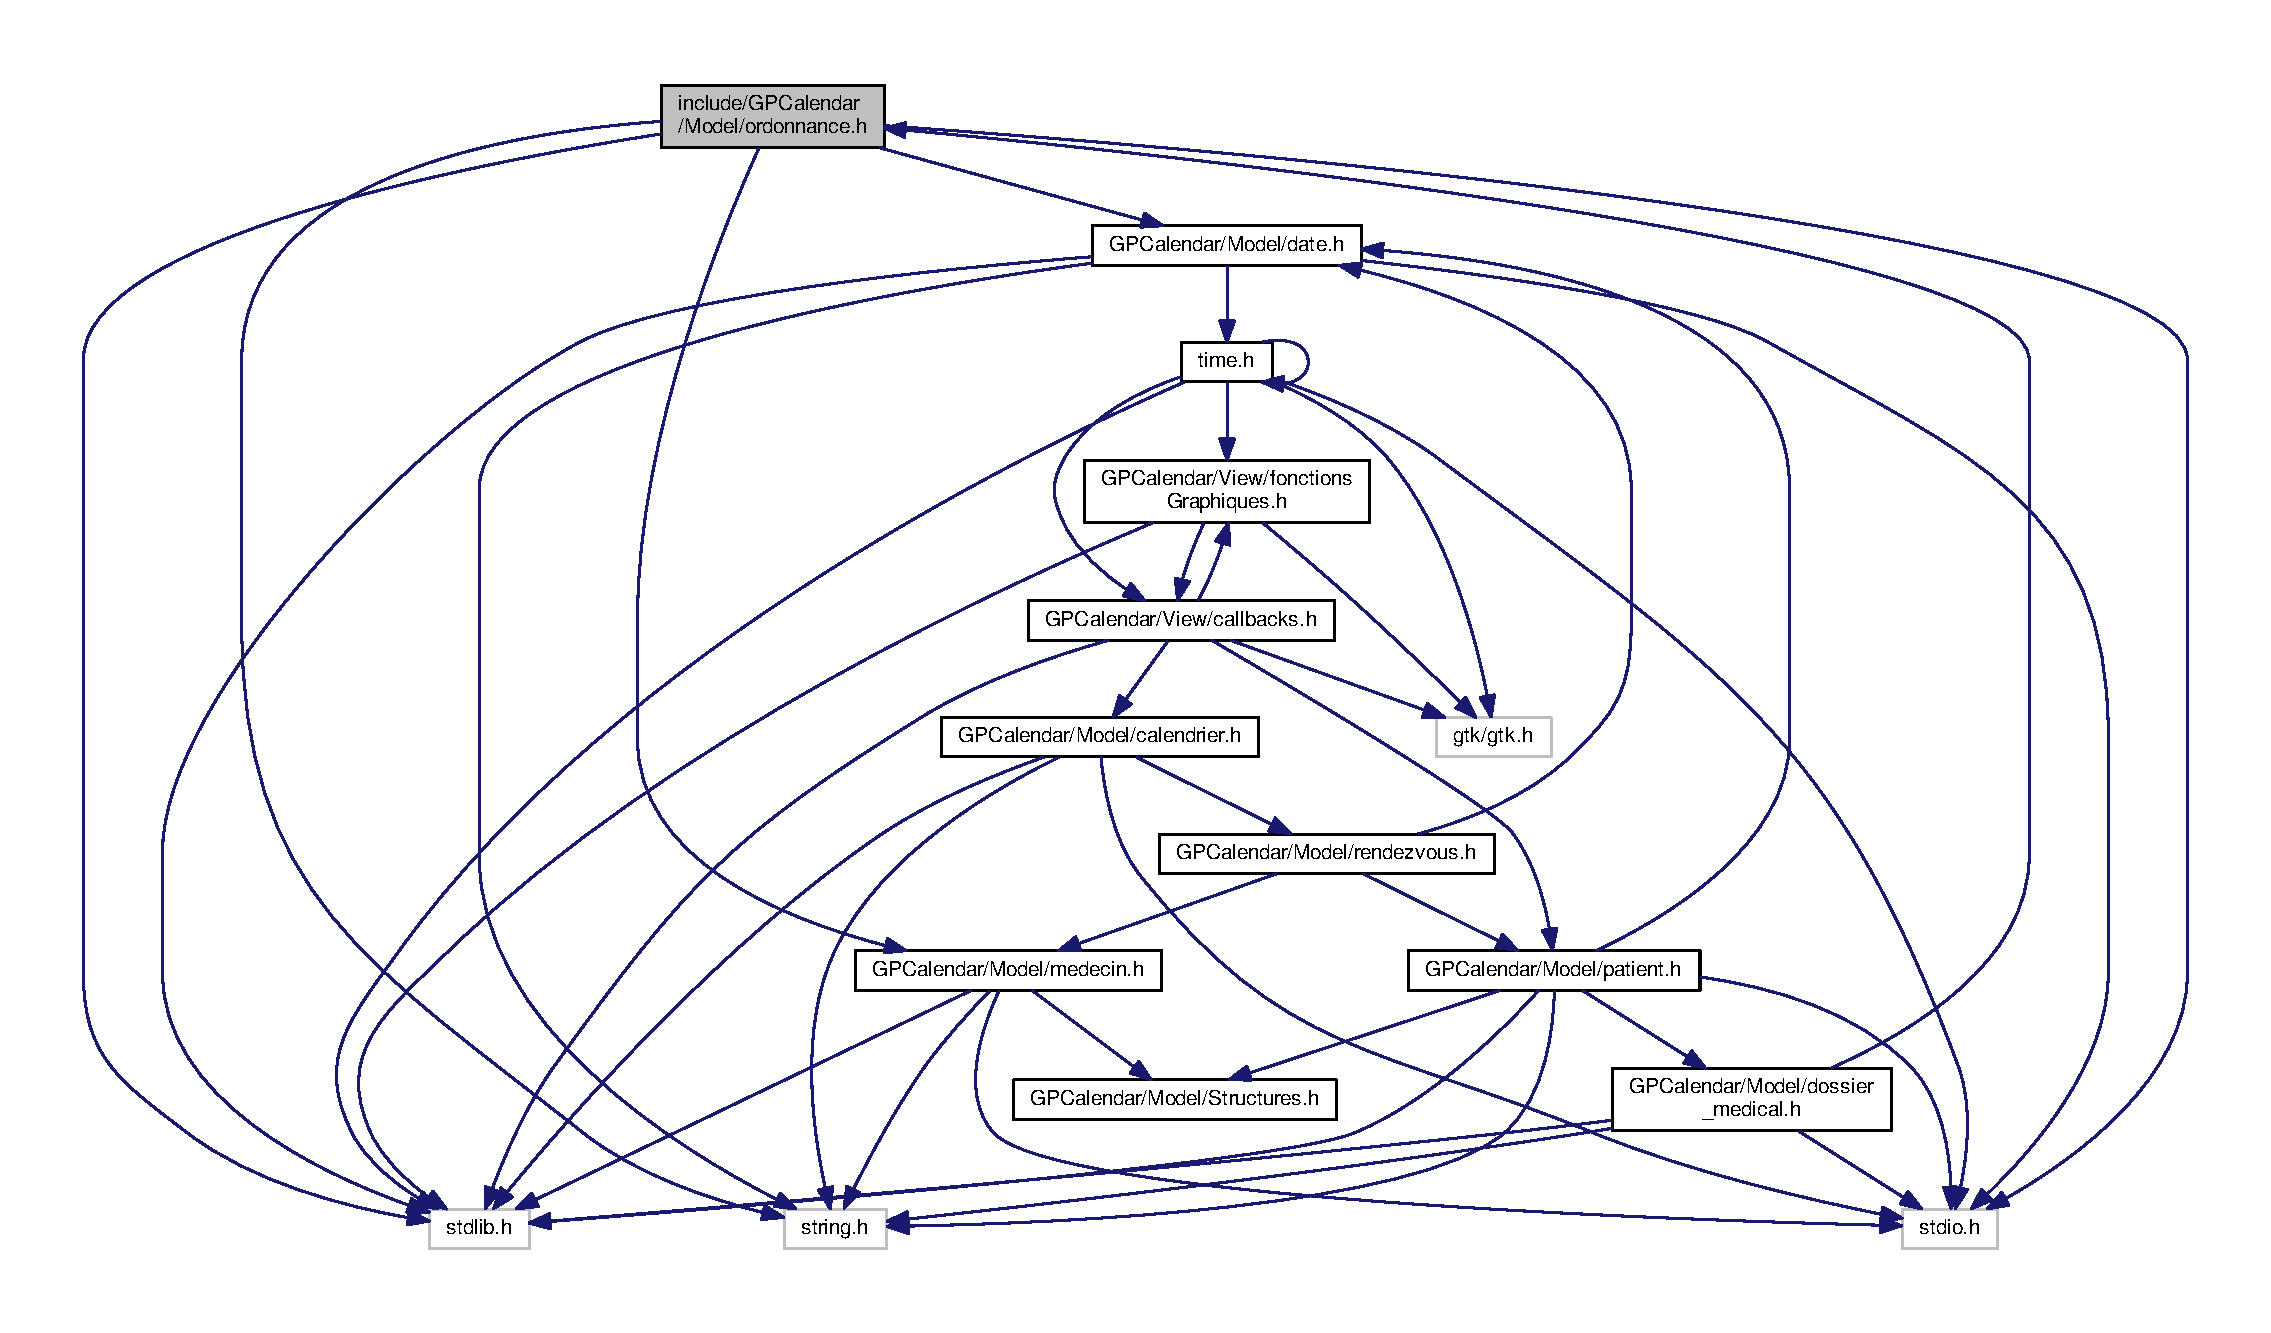
\includegraphics[width=350pt]{ordonnance_8h__incl}
\end{center}
\end{figure}
Ce graphe montre quels fichiers incluent directement ou indirectement ce fichier \-:
\nopagebreak
\begin{figure}[H]
\begin{center}
\leavevmode
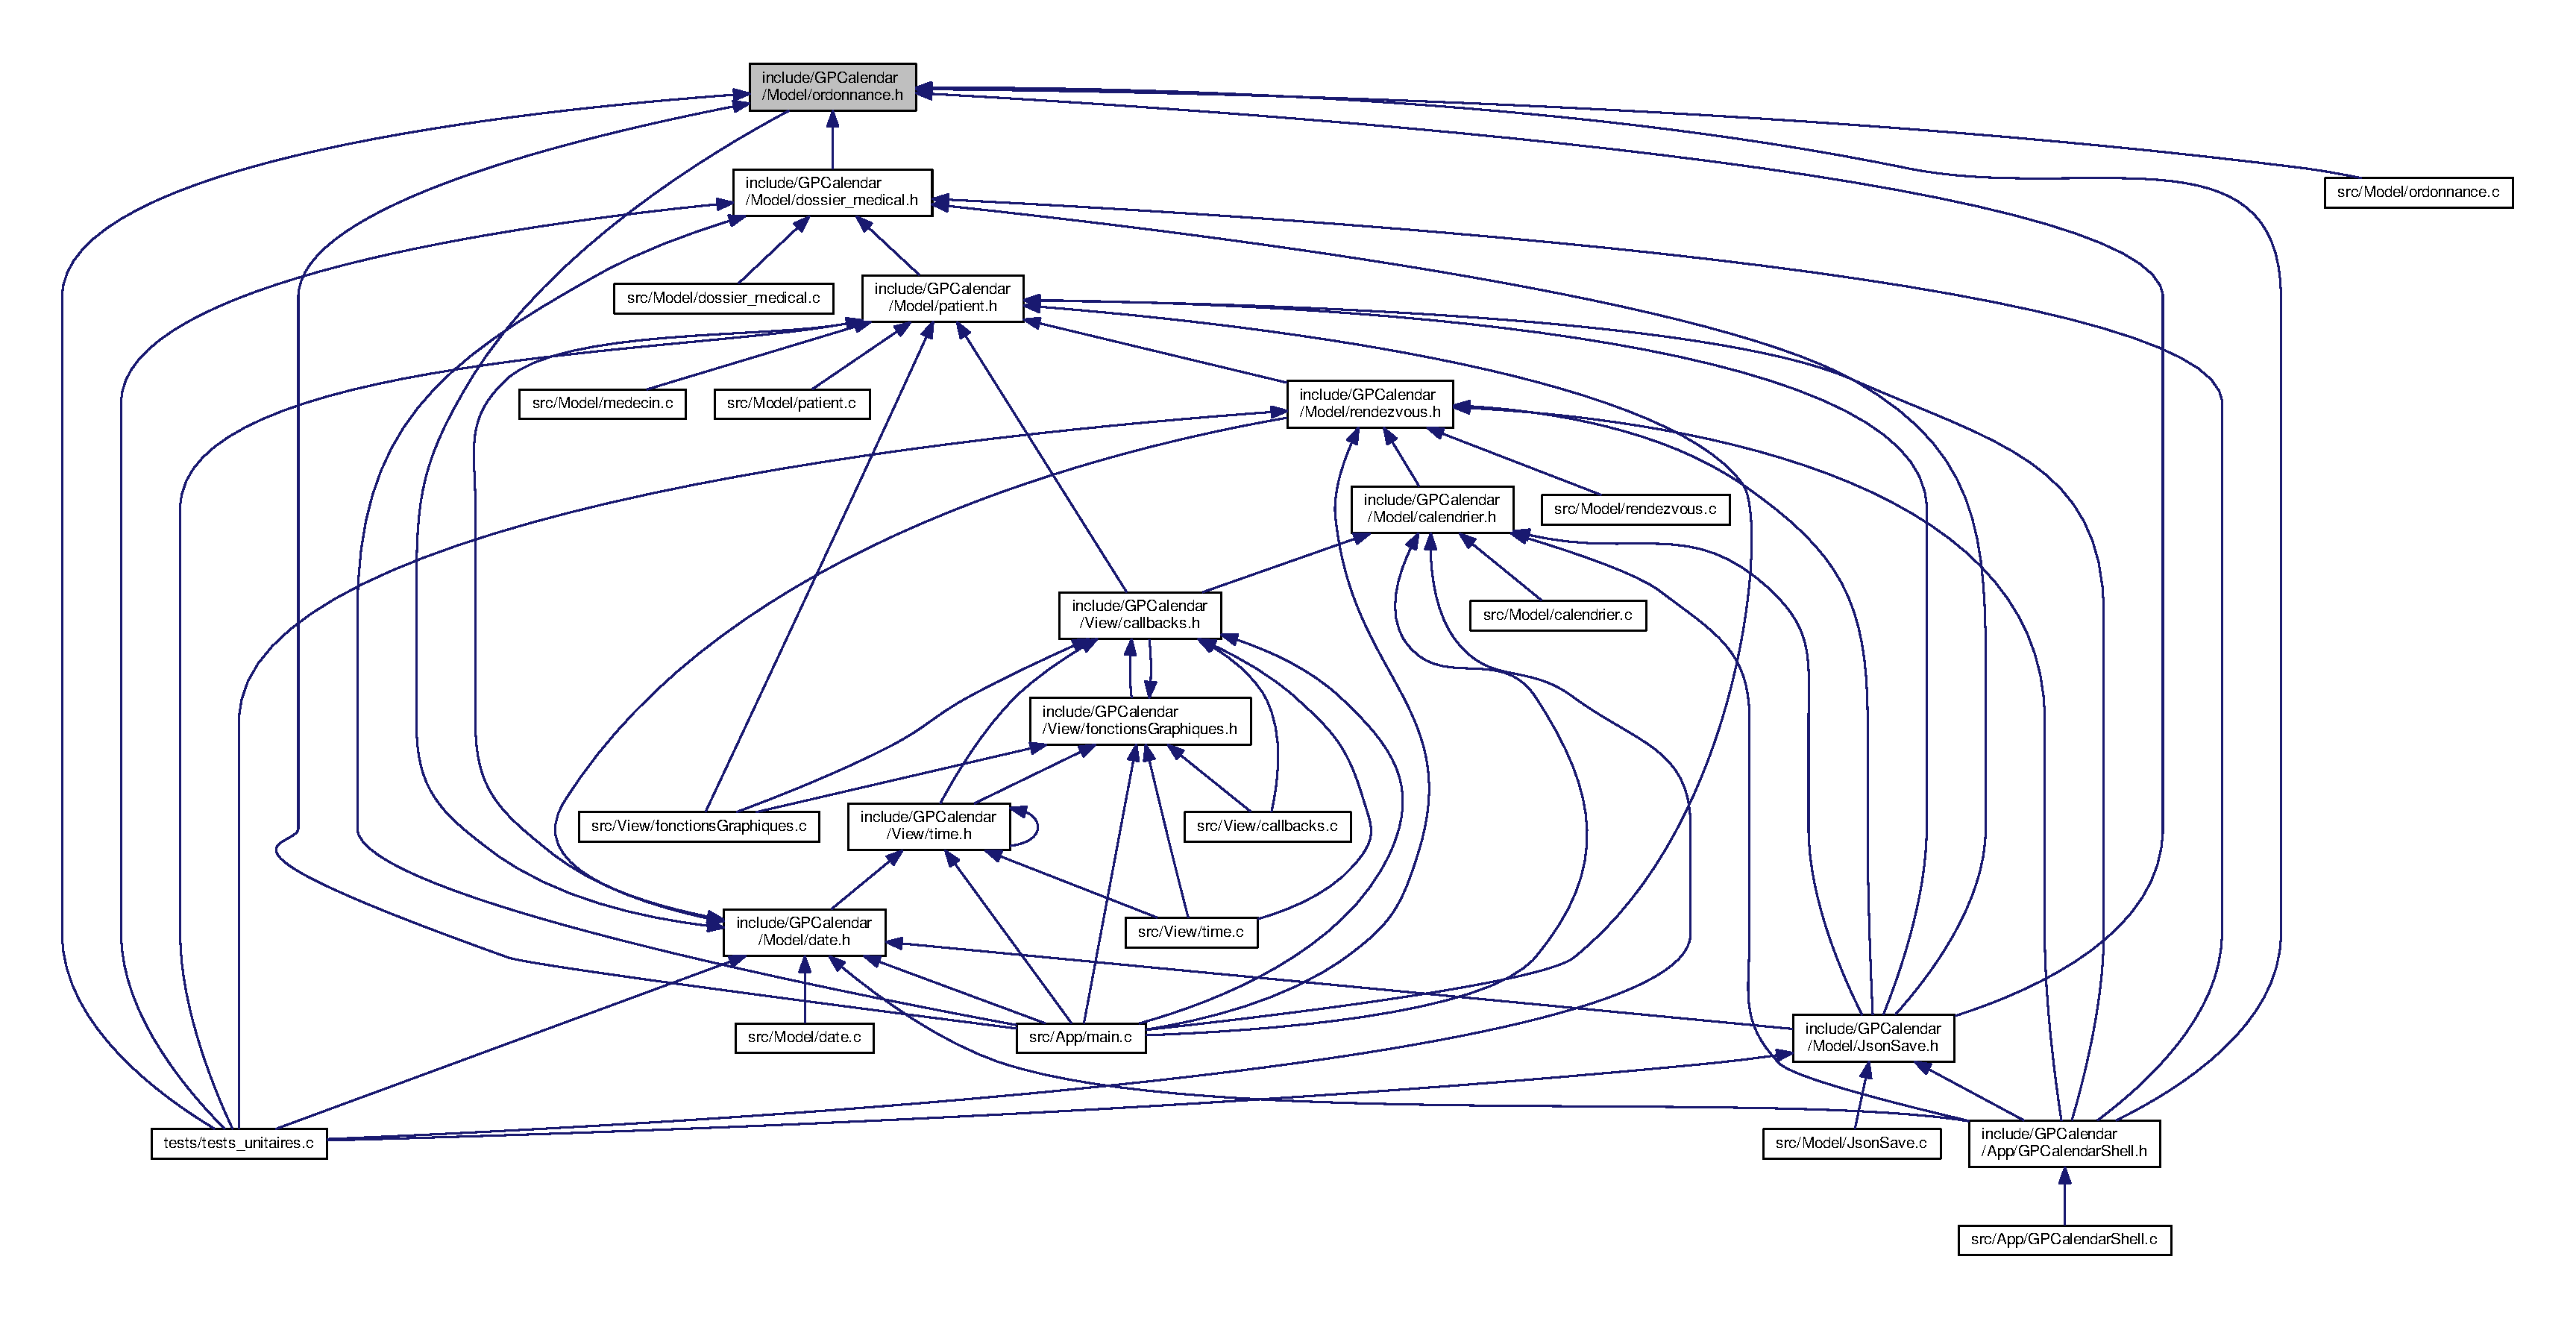
\includegraphics[width=350pt]{ordonnance_8h__dep__incl}
\end{center}
\end{figure}
\subsection*{Structures de données}
\begin{DoxyCompactItemize}
\item 
struct \hyperlink{struct_ordonnance}{Ordonnance}
\item 
struct \hyperlink{struct_node_ordonnance}{Node\-Ordonnance}
\item 
struct \hyperlink{struct_list_ordonnance}{List\-Ordonnance}
\end{DoxyCompactItemize}
\subsection*{Définitions de type}
\begin{DoxyCompactItemize}
\item 
typedef struct \hyperlink{struct_node_ordonnance}{Node\-Ordonnance} \hyperlink{ordonnance_8h_aa21777b78b86a2852a16260404a5e662}{Node\-Ordonnance}
\end{DoxyCompactItemize}
\subsection*{Fonctions}
\begin{DoxyCompactItemize}
\item 
\hyperlink{struct_ordonnance}{Ordonnance} $\ast$ \hyperlink{ordonnance_8h_ab80465380858194f28db009b8cd305fd}{Creer\-Ordonnance} (\hyperlink{struct_medecin}{Medecin} $\ast$m, char $\ast$description)
\item 
\hyperlink{struct_ordonnance}{Ordonnance} $\ast$ \hyperlink{ordonnance_8h_a0a7106efdac4dac48a3654833fa0f963}{Load\-Ordonnance} (\hyperlink{struct_medecin}{Medecin} $\ast$medecin, int date\-\_\-edi\-\_\-jour, int date\-\_\-edi\-\_\-mois, int date\-\_\-edi\-\_\-annee, int date\-\_\-expi\-\_\-jour, int date\-\_\-expi\-\_\-mois, int date\-\_\-expi\-\_\-annee, char $\ast$description)
\item 
void \hyperlink{ordonnance_8h_a896ca490c0275822a13514c8248d277d}{Delete\-Ordonnance} (\hyperlink{struct_ordonnance}{Ordonnance} $\ast$o)
\item 
int \hyperlink{ordonnance_8h_aa94cf1a1467605f806b896f0ef8a34bd}{modifier\-Ordonnance} (\hyperlink{struct_ordonnance}{Ordonnance} $\ast$ordo, \hyperlink{struct_medecin}{Medecin} $\ast$m, char $\ast$description)
\item 
void \hyperlink{ordonnance_8h_ac59dd8024ed866b917e09ca8de7ef5ae}{print\-Ordonnance} (char $\ast$infos, \hyperlink{struct_ordonnance}{Ordonnance} $\ast$ordo)
\item 
\hyperlink{struct_node_ordonnance}{Node\-Ordonnance} $\ast$ \hyperlink{ordonnance_8h_a8f765b7edc568e61ef4f6a8f9acc5da2}{new\-Node\-Ordonnance} (\hyperlink{struct_ordonnance}{Ordonnance} $\ast$o, \hyperlink{struct_node_ordonnance}{Node\-Ordonnance} $\ast$previous, \hyperlink{struct_node_ordonnance}{Node\-Ordonnance} $\ast$next)
\item 
void \hyperlink{ordonnance_8h_a870956eab1e669be1956d4da5a75c51c}{free\-Node\-Ordonnance} (\hyperlink{struct_list_ordonnance}{List\-Ordonnance} $\ast$l, \hyperlink{struct_node_ordonnance}{Node\-Ordonnance} $\ast$n)
\item 
void \hyperlink{ordonnance_8h_ad40e3d193cdc208b3bf052457c2557db}{free\-Node\-Ordonnance\-\_\-without\-Deleting\-Ordonnance} (\hyperlink{struct_list_ordonnance}{List\-Ordonnance} $\ast$l, \hyperlink{struct_node_ordonnance}{Node\-Ordonnance} $\ast$n)
\item 
void \hyperlink{ordonnance_8h_ae41a4766285c1bf190f73beda51b26b1}{List\-Ordonnance\-\_\-init} (\hyperlink{struct_list_ordonnance}{List\-Ordonnance} $\ast$l)
\item 
void \hyperlink{ordonnance_8h_ab2374a904522f810e38a96ab2b70a96b}{List\-Ordonnance\-\_\-free} (\hyperlink{struct_list_ordonnance}{List\-Ordonnance} $\ast$l)
\item 
void \hyperlink{ordonnance_8h_ada3306a875d73fdbc4c597335cb8648a}{List\-Ordonnance\-\_\-free\-\_\-without\-Deleting\-Ordonnance} (\hyperlink{struct_list_ordonnance}{List\-Ordonnance} $\ast$l)
\item 
int \hyperlink{ordonnance_8h_ad36331d7ecda656771d1560d3015ca08}{List\-Ordonnance\-\_\-is\-Empty} (\hyperlink{struct_list_ordonnance}{List\-Ordonnance} $\ast$l)
\item 
int \hyperlink{ordonnance_8h_ad16d6389aa9f75d7a4642fdd0f47ce75}{List\-Ordonnance\-\_\-is\-First} (\hyperlink{struct_list_ordonnance}{List\-Ordonnance} $\ast$l)
\item 
int \hyperlink{ordonnance_8h_a274c3a2b9f3497657df33212a41cece7}{List\-Ordonnance\-\_\-is\-Last} (\hyperlink{struct_list_ordonnance}{List\-Ordonnance} $\ast$l)
\item 
int \hyperlink{ordonnance_8h_a1467b36f1510a920d26c7f47934c732d}{List\-Ordonnance\-\_\-is\-Out\-Of\-List} (\hyperlink{struct_list_ordonnance}{List\-Ordonnance} $\ast$l)
\item 
void \hyperlink{ordonnance_8h_add110561a476b06a4666aca1e1873518}{List\-Ordonnance\-\_\-set\-On\-First} (\hyperlink{struct_list_ordonnance}{List\-Ordonnance} $\ast$l)
\item 
void \hyperlink{ordonnance_8h_acd59abef86cb57ef0c75847488ce817d}{List\-Ordonnance\-\_\-set\-On\-Last} (\hyperlink{struct_list_ordonnance}{List\-Ordonnance} $\ast$l)
\item 
void \hyperlink{ordonnance_8h_a6eac0d9f4066e9f674590a8b85a02bc8}{List\-Ordonnance\-\_\-set\-On\-Next} (\hyperlink{struct_list_ordonnance}{List\-Ordonnance} $\ast$l)
\item 
void \hyperlink{ordonnance_8h_a05fb637a10a8c2cea759faedde76d0fd}{List\-Ordonnance\-\_\-set\-On\-Previous} (\hyperlink{struct_list_ordonnance}{List\-Ordonnance} $\ast$l)
\item 
\hyperlink{struct_ordonnance}{Ordonnance} $\ast$ \hyperlink{ordonnance_8h_a4a12cc83df7aa0debd28203bde798721}{List\-Ordonnance\-\_\-get\-Current} (\hyperlink{struct_list_ordonnance}{List\-Ordonnance} $\ast$l)
\end{DoxyCompactItemize}


\subsection{Documentation des définitions de type}
\hypertarget{ordonnance_8h_aa21777b78b86a2852a16260404a5e662}{\index{ordonnance.\-h@{ordonnance.\-h}!Node\-Ordonnance@{Node\-Ordonnance}}
\index{Node\-Ordonnance@{Node\-Ordonnance}!ordonnance.h@{ordonnance.\-h}}
\subsubsection[{Node\-Ordonnance}]{\setlength{\rightskip}{0pt plus 5cm}typedef struct {\bf Node\-Ordonnance} {\bf Node\-Ordonnance}}}\label{ordonnance_8h_aa21777b78b86a2852a16260404a5e662}
Structure \hyperlink{struct_node_ordonnance}{Node\-Ordonnance} 

\subsection{Documentation des fonctions}
\hypertarget{ordonnance_8h_ab80465380858194f28db009b8cd305fd}{\index{ordonnance.\-h@{ordonnance.\-h}!Creer\-Ordonnance@{Creer\-Ordonnance}}
\index{Creer\-Ordonnance@{Creer\-Ordonnance}!ordonnance.h@{ordonnance.\-h}}
\subsubsection[{Creer\-Ordonnance}]{\setlength{\rightskip}{0pt plus 5cm}{\bf Ordonnance}$\ast$ Creer\-Ordonnance (
\begin{DoxyParamCaption}
\item[{{\bf Medecin} $\ast$}]{m, }
\item[{char $\ast$}]{description}
\end{DoxyParamCaption}
)}}\label{ordonnance_8h_ab80465380858194f28db009b8cd305fd}
Creer\-Ordonnance \-: Creer dynamiquement un objet \hyperlink{struct_ordonnance}{Ordonnance} 
\begin{DoxyParams}{Paramètres}
{\em patient} & \-: le patient concerné par l'ordonnance \\
\hline
{\em medecin} & \-: le medecin qui prescrit l'ordonnance \\
\hline
{\em description} & \-: description de la prescription \\
\hline
\end{DoxyParams}
\begin{DoxyReturn}{Renvoie}
l'ordonnance créée 
\end{DoxyReturn}
\hypertarget{ordonnance_8h_a896ca490c0275822a13514c8248d277d}{\index{ordonnance.\-h@{ordonnance.\-h}!Delete\-Ordonnance@{Delete\-Ordonnance}}
\index{Delete\-Ordonnance@{Delete\-Ordonnance}!ordonnance.h@{ordonnance.\-h}}
\subsubsection[{Delete\-Ordonnance}]{\setlength{\rightskip}{0pt plus 5cm}void Delete\-Ordonnance (
\begin{DoxyParamCaption}
\item[{{\bf Ordonnance} $\ast$}]{o}
\end{DoxyParamCaption}
)}}\label{ordonnance_8h_a896ca490c0275822a13514c8248d277d}
Delete\-Ordonnance \-: Free un objet ordonnance 
\begin{DoxyParams}{Paramètres}
{\em o} & \-: l'ordonnance à supprimer \\
\hline
\end{DoxyParams}
\hypertarget{ordonnance_8h_a870956eab1e669be1956d4da5a75c51c}{\index{ordonnance.\-h@{ordonnance.\-h}!free\-Node\-Ordonnance@{free\-Node\-Ordonnance}}
\index{free\-Node\-Ordonnance@{free\-Node\-Ordonnance}!ordonnance.h@{ordonnance.\-h}}
\subsubsection[{free\-Node\-Ordonnance}]{\setlength{\rightskip}{0pt plus 5cm}void free\-Node\-Ordonnance (
\begin{DoxyParamCaption}
\item[{{\bf List\-Ordonnance} $\ast$}]{l, }
\item[{{\bf Node\-Ordonnance} $\ast$}]{n}
\end{DoxyParamCaption}
)}}\label{ordonnance_8h_a870956eab1e669be1956d4da5a75c51c}
free\-Node\-Ordonnance \-: Permet de delete proprement (avec un free) un \hyperlink{struct_node_ordonnance}{Node\-Ordonnance} 
\begin{DoxyParams}{Paramètres}
{\em n} & \-: le node à delete \\
\hline
\end{DoxyParams}
\hypertarget{ordonnance_8h_ad40e3d193cdc208b3bf052457c2557db}{\index{ordonnance.\-h@{ordonnance.\-h}!free\-Node\-Ordonnance\-\_\-without\-Deleting\-Ordonnance@{free\-Node\-Ordonnance\-\_\-without\-Deleting\-Ordonnance}}
\index{free\-Node\-Ordonnance\-\_\-without\-Deleting\-Ordonnance@{free\-Node\-Ordonnance\-\_\-without\-Deleting\-Ordonnance}!ordonnance.h@{ordonnance.\-h}}
\subsubsection[{free\-Node\-Ordonnance\-\_\-without\-Deleting\-Ordonnance}]{\setlength{\rightskip}{0pt plus 5cm}void free\-Node\-Ordonnance\-\_\-without\-Deleting\-Ordonnance (
\begin{DoxyParamCaption}
\item[{{\bf List\-Ordonnance} $\ast$}]{l, }
\item[{{\bf Node\-Ordonnance} $\ast$}]{n}
\end{DoxyParamCaption}
)}}\label{ordonnance_8h_ad40e3d193cdc208b3bf052457c2557db}
free\-Node\-Ordonnance\-\_\-without\-Deleting\-Ordonnance \-: Permet de delete un node\-Ordonnance mais sans delete l'ordonnance liée au node 
\begin{DoxyParams}{Paramètres}
{\em n} & \-: le node à delete \\
\hline
\end{DoxyParams}
\hypertarget{ordonnance_8h_ab2374a904522f810e38a96ab2b70a96b}{\index{ordonnance.\-h@{ordonnance.\-h}!List\-Ordonnance\-\_\-free@{List\-Ordonnance\-\_\-free}}
\index{List\-Ordonnance\-\_\-free@{List\-Ordonnance\-\_\-free}!ordonnance.h@{ordonnance.\-h}}
\subsubsection[{List\-Ordonnance\-\_\-free}]{\setlength{\rightskip}{0pt plus 5cm}void List\-Ordonnance\-\_\-free (
\begin{DoxyParamCaption}
\item[{{\bf List\-Ordonnance} $\ast$}]{l}
\end{DoxyParamCaption}
)}}\label{ordonnance_8h_ab2374a904522f810e38a96ab2b70a96b}
List\-Ordonnance\-\_\-free \-: Libère la mémoire occupée par l'objet \hyperlink{struct_list_ordonnance}{List\-Ordonnance} passé en paramètre 
\begin{DoxyParams}{Paramètres}
{\em l} & \-: la liste de ordonnances à free \\
\hline
\end{DoxyParams}
\hypertarget{ordonnance_8h_ada3306a875d73fdbc4c597335cb8648a}{\index{ordonnance.\-h@{ordonnance.\-h}!List\-Ordonnance\-\_\-free\-\_\-without\-Deleting\-Ordonnance@{List\-Ordonnance\-\_\-free\-\_\-without\-Deleting\-Ordonnance}}
\index{List\-Ordonnance\-\_\-free\-\_\-without\-Deleting\-Ordonnance@{List\-Ordonnance\-\_\-free\-\_\-without\-Deleting\-Ordonnance}!ordonnance.h@{ordonnance.\-h}}
\subsubsection[{List\-Ordonnance\-\_\-free\-\_\-without\-Deleting\-Ordonnance}]{\setlength{\rightskip}{0pt plus 5cm}void List\-Ordonnance\-\_\-free\-\_\-without\-Deleting\-Ordonnance (
\begin{DoxyParamCaption}
\item[{{\bf List\-Ordonnance} $\ast$}]{l}
\end{DoxyParamCaption}
)}}\label{ordonnance_8h_ada3306a875d73fdbc4c597335cb8648a}
List\-Ordonnance\-\_\-free\-\_\-without\-Deleting\-Ordonnance \-: Libère la mémoire occupée par l'objet \hyperlink{struct_list_ordonnance}{List\-Ordonnance} passé en paramètre mais sans delete les ordonnances de cette liste (uniquement les nodes) 
\begin{DoxyParams}{Paramètres}
{\em l} & \-: la liste d'ordonnances à free \\
\hline
\end{DoxyParams}
\hypertarget{ordonnance_8h_a4a12cc83df7aa0debd28203bde798721}{\index{ordonnance.\-h@{ordonnance.\-h}!List\-Ordonnance\-\_\-get\-Current@{List\-Ordonnance\-\_\-get\-Current}}
\index{List\-Ordonnance\-\_\-get\-Current@{List\-Ordonnance\-\_\-get\-Current}!ordonnance.h@{ordonnance.\-h}}
\subsubsection[{List\-Ordonnance\-\_\-get\-Current}]{\setlength{\rightskip}{0pt plus 5cm}{\bf Ordonnance}$\ast$ List\-Ordonnance\-\_\-get\-Current (
\begin{DoxyParamCaption}
\item[{{\bf List\-Ordonnance} $\ast$}]{l}
\end{DoxyParamCaption}
)}}\label{ordonnance_8h_a4a12cc83df7aa0debd28203bde798721}
List\-Ordonnance\-\_\-get\-Current \-: Permet d'acceder à l'\hyperlink{struct_ordonnance}{Ordonnance} pointée par current 
\begin{DoxyParams}{Paramètres}
{\em l} & \-: la liste \\
\hline
\end{DoxyParams}
\begin{DoxyReturn}{Renvoie}
Retourne un pointeur sur l'\hyperlink{struct_ordonnance}{Ordonnance} de l'élément courant de la liste 
\end{DoxyReturn}
\hypertarget{ordonnance_8h_ae41a4766285c1bf190f73beda51b26b1}{\index{ordonnance.\-h@{ordonnance.\-h}!List\-Ordonnance\-\_\-init@{List\-Ordonnance\-\_\-init}}
\index{List\-Ordonnance\-\_\-init@{List\-Ordonnance\-\_\-init}!ordonnance.h@{ordonnance.\-h}}
\subsubsection[{List\-Ordonnance\-\_\-init}]{\setlength{\rightskip}{0pt plus 5cm}void List\-Ordonnance\-\_\-init (
\begin{DoxyParamCaption}
\item[{{\bf List\-Ordonnance} $\ast$}]{l}
\end{DoxyParamCaption}
)}}\label{ordonnance_8h_ae41a4766285c1bf190f73beda51b26b1}
List\-Ordonnance\-\_\-init \-: Initialise correctement une liste de \hyperlink{struct_node_ordonnance}{Node\-Ordonnance} en reliant sentinel\-\_\-begin et end entre eux et en mettant current à N\-U\-L\-L (en dehors de la liste) 
\begin{DoxyParams}{Paramètres}
{\em l} & \-: la liste à initialiser \\
\hline
\end{DoxyParams}
\hypertarget{ordonnance_8h_ad36331d7ecda656771d1560d3015ca08}{\index{ordonnance.\-h@{ordonnance.\-h}!List\-Ordonnance\-\_\-is\-Empty@{List\-Ordonnance\-\_\-is\-Empty}}
\index{List\-Ordonnance\-\_\-is\-Empty@{List\-Ordonnance\-\_\-is\-Empty}!ordonnance.h@{ordonnance.\-h}}
\subsubsection[{List\-Ordonnance\-\_\-is\-Empty}]{\setlength{\rightskip}{0pt plus 5cm}int List\-Ordonnance\-\_\-is\-Empty (
\begin{DoxyParamCaption}
\item[{{\bf List\-Ordonnance} $\ast$}]{l}
\end{DoxyParamCaption}
)}}\label{ordonnance_8h_ad36331d7ecda656771d1560d3015ca08}
List\-Ordonnance\-\_\-is\-Empty \-: Vérifie si la liste de \hyperlink{struct_ordonnance}{Ordonnance} est vide ou non 
\begin{DoxyParams}{Paramètres}
{\em l} & \-: la liste \\
\hline
\end{DoxyParams}
\begin{DoxyReturn}{Renvoie}
1 si la liste est vide 0 si elle ne l'est pas -\/1 si la liste est N\-U\-L\-L 
\end{DoxyReturn}
\hypertarget{ordonnance_8h_ad16d6389aa9f75d7a4642fdd0f47ce75}{\index{ordonnance.\-h@{ordonnance.\-h}!List\-Ordonnance\-\_\-is\-First@{List\-Ordonnance\-\_\-is\-First}}
\index{List\-Ordonnance\-\_\-is\-First@{List\-Ordonnance\-\_\-is\-First}!ordonnance.h@{ordonnance.\-h}}
\subsubsection[{List\-Ordonnance\-\_\-is\-First}]{\setlength{\rightskip}{0pt plus 5cm}int List\-Ordonnance\-\_\-is\-First (
\begin{DoxyParamCaption}
\item[{{\bf List\-Ordonnance} $\ast$}]{l}
\end{DoxyParamCaption}
)}}\label{ordonnance_8h_ad16d6389aa9f75d7a4642fdd0f47ce75}
List\-Ordonnance\-\_\-is\-First \-: Vérifie si current est positionné sur le premier élément de la liste 
\begin{DoxyParams}{Paramètres}
{\em l} & \-: la liste \\
\hline
\end{DoxyParams}
\begin{DoxyReturn}{Renvoie}
1 si current est bien sur le premier élément 0 si il ne l'est pas -\/1 si la liste est N\-U\-L\-L 
\end{DoxyReturn}
\hypertarget{ordonnance_8h_a274c3a2b9f3497657df33212a41cece7}{\index{ordonnance.\-h@{ordonnance.\-h}!List\-Ordonnance\-\_\-is\-Last@{List\-Ordonnance\-\_\-is\-Last}}
\index{List\-Ordonnance\-\_\-is\-Last@{List\-Ordonnance\-\_\-is\-Last}!ordonnance.h@{ordonnance.\-h}}
\subsubsection[{List\-Ordonnance\-\_\-is\-Last}]{\setlength{\rightskip}{0pt plus 5cm}int List\-Ordonnance\-\_\-is\-Last (
\begin{DoxyParamCaption}
\item[{{\bf List\-Ordonnance} $\ast$}]{l}
\end{DoxyParamCaption}
)}}\label{ordonnance_8h_a274c3a2b9f3497657df33212a41cece7}
List\-Ordonnance\-\_\-is\-Last \-: Vérifie si current est positionné sur le dernier élément de la liste 
\begin{DoxyParams}{Paramètres}
{\em l} & \-: la liste \\
\hline
\end{DoxyParams}
\begin{DoxyReturn}{Renvoie}
1 si current est bien sur le dernier élément 0 si il ne l'est pas -\/1 si la liste est N\-U\-L\-L 
\end{DoxyReturn}
\hypertarget{ordonnance_8h_a1467b36f1510a920d26c7f47934c732d}{\index{ordonnance.\-h@{ordonnance.\-h}!List\-Ordonnance\-\_\-is\-Out\-Of\-List@{List\-Ordonnance\-\_\-is\-Out\-Of\-List}}
\index{List\-Ordonnance\-\_\-is\-Out\-Of\-List@{List\-Ordonnance\-\_\-is\-Out\-Of\-List}!ordonnance.h@{ordonnance.\-h}}
\subsubsection[{List\-Ordonnance\-\_\-is\-Out\-Of\-List}]{\setlength{\rightskip}{0pt plus 5cm}int List\-Ordonnance\-\_\-is\-Out\-Of\-List (
\begin{DoxyParamCaption}
\item[{{\bf List\-Ordonnance} $\ast$}]{l}
\end{DoxyParamCaption}
)}}\label{ordonnance_8h_a1467b36f1510a920d26c7f47934c732d}
List\-Ordonnance\-\_\-is\-Out\-Of\-List \-: Vérifie si current est bien placé sur un élément de la liste (les sentinels ne sont pas considérées comme dans la liste) 
\begin{DoxyParams}{Paramètres}
{\em l} & \-: la liste \\
\hline
\end{DoxyParams}
\begin{DoxyReturn}{Renvoie}
1 si current vaut N\-U\-L\-L 0 sinon -\/1 si la liste est N\-U\-L\-L 
\end{DoxyReturn}
\hypertarget{ordonnance_8h_add110561a476b06a4666aca1e1873518}{\index{ordonnance.\-h@{ordonnance.\-h}!List\-Ordonnance\-\_\-set\-On\-First@{List\-Ordonnance\-\_\-set\-On\-First}}
\index{List\-Ordonnance\-\_\-set\-On\-First@{List\-Ordonnance\-\_\-set\-On\-First}!ordonnance.h@{ordonnance.\-h}}
\subsubsection[{List\-Ordonnance\-\_\-set\-On\-First}]{\setlength{\rightskip}{0pt plus 5cm}void List\-Ordonnance\-\_\-set\-On\-First (
\begin{DoxyParamCaption}
\item[{{\bf List\-Ordonnance} $\ast$}]{l}
\end{DoxyParamCaption}
)}}\label{ordonnance_8h_add110561a476b06a4666aca1e1873518}
List\-Ordonnance\-\_\-set\-On\-First \-: Positionne le pointeur courant sur le premier élément de la liste 
\begin{DoxyParams}{Paramètres}
{\em l} & \-: la liste \\
\hline
\end{DoxyParams}
\hypertarget{ordonnance_8h_acd59abef86cb57ef0c75847488ce817d}{\index{ordonnance.\-h@{ordonnance.\-h}!List\-Ordonnance\-\_\-set\-On\-Last@{List\-Ordonnance\-\_\-set\-On\-Last}}
\index{List\-Ordonnance\-\_\-set\-On\-Last@{List\-Ordonnance\-\_\-set\-On\-Last}!ordonnance.h@{ordonnance.\-h}}
\subsubsection[{List\-Ordonnance\-\_\-set\-On\-Last}]{\setlength{\rightskip}{0pt plus 5cm}void List\-Ordonnance\-\_\-set\-On\-Last (
\begin{DoxyParamCaption}
\item[{{\bf List\-Ordonnance} $\ast$}]{l}
\end{DoxyParamCaption}
)}}\label{ordonnance_8h_acd59abef86cb57ef0c75847488ce817d}
List\-Ordonnance\-\_\-set\-On\-Last \-: Positionne le pointeur courant sur le dernier élément de la liste 
\begin{DoxyParams}{Paramètres}
{\em l} & \-: la liste \\
\hline
\end{DoxyParams}
\hypertarget{ordonnance_8h_a6eac0d9f4066e9f674590a8b85a02bc8}{\index{ordonnance.\-h@{ordonnance.\-h}!List\-Ordonnance\-\_\-set\-On\-Next@{List\-Ordonnance\-\_\-set\-On\-Next}}
\index{List\-Ordonnance\-\_\-set\-On\-Next@{List\-Ordonnance\-\_\-set\-On\-Next}!ordonnance.h@{ordonnance.\-h}}
\subsubsection[{List\-Ordonnance\-\_\-set\-On\-Next}]{\setlength{\rightskip}{0pt plus 5cm}void List\-Ordonnance\-\_\-set\-On\-Next (
\begin{DoxyParamCaption}
\item[{{\bf List\-Ordonnance} $\ast$}]{l}
\end{DoxyParamCaption}
)}}\label{ordonnance_8h_a6eac0d9f4066e9f674590a8b85a02bc8}
List\-Ordonnance\-\_\-set\-On\-Next \-: Positionne le pointeur courant sur le prochain élément de la liste 
\begin{DoxyParams}{Paramètres}
{\em l} & \-: la liste \\
\hline
\end{DoxyParams}
\hypertarget{ordonnance_8h_a05fb637a10a8c2cea759faedde76d0fd}{\index{ordonnance.\-h@{ordonnance.\-h}!List\-Ordonnance\-\_\-set\-On\-Previous@{List\-Ordonnance\-\_\-set\-On\-Previous}}
\index{List\-Ordonnance\-\_\-set\-On\-Previous@{List\-Ordonnance\-\_\-set\-On\-Previous}!ordonnance.h@{ordonnance.\-h}}
\subsubsection[{List\-Ordonnance\-\_\-set\-On\-Previous}]{\setlength{\rightskip}{0pt plus 5cm}void List\-Ordonnance\-\_\-set\-On\-Previous (
\begin{DoxyParamCaption}
\item[{{\bf List\-Ordonnance} $\ast$}]{l}
\end{DoxyParamCaption}
)}}\label{ordonnance_8h_a05fb637a10a8c2cea759faedde76d0fd}
List\-Ordonnance\-\_\-set\-On\-Previous \-: Positionne le pointeur courant sur l'élément le précédant dans la liste 
\begin{DoxyParams}{Paramètres}
{\em l} & \-: la liste \\
\hline
\end{DoxyParams}
\hypertarget{ordonnance_8h_a0a7106efdac4dac48a3654833fa0f963}{\index{ordonnance.\-h@{ordonnance.\-h}!Load\-Ordonnance@{Load\-Ordonnance}}
\index{Load\-Ordonnance@{Load\-Ordonnance}!ordonnance.h@{ordonnance.\-h}}
\subsubsection[{Load\-Ordonnance}]{\setlength{\rightskip}{0pt plus 5cm}{\bf Ordonnance}$\ast$ Load\-Ordonnance (
\begin{DoxyParamCaption}
\item[{{\bf Medecin} $\ast$}]{medecin, }
\item[{int}]{date\-\_\-edi\-\_\-jour, }
\item[{int}]{date\-\_\-edi\-\_\-mois, }
\item[{int}]{date\-\_\-edi\-\_\-annee, }
\item[{int}]{date\-\_\-expi\-\_\-jour, }
\item[{int}]{date\-\_\-expi\-\_\-mois, }
\item[{int}]{date\-\_\-expi\-\_\-annee, }
\item[{char $\ast$}]{description}
\end{DoxyParamCaption}
)}}\label{ordonnance_8h_a0a7106efdac4dac48a3654833fa0f963}
Load\-Ordonnance \-: Fonction utilisée lors du load d'un projet J\-S\-O\-N, initialise une ordonnance avec son pointeur sur le mèdecin à N\-U\-L\-L mais avec num\-R\-P\-S\-Medecin avec le num R\-P\-S du mèdecin, il faudra donc aller chercher le mèdecin correspondant plus tard et avec les bonnes dates (pas la courante et celle 3 mois plus tard) \-: l'ordonnance ne date pas forcément du jour présent, elle peut être plus vieille 
\begin{DoxyParams}{Paramètres}
{\em rps\-Medecin} & \-: le num R\-P\-S du mèdecin ayant fait l'ordonnance\\
\hline
{\em date\-\_\-edi\-\_\-jour} & $\vert$ \\
\hline
{\em date\-\_\-edi\-\_\-mois} & $\vert$ ---$>$ La date d'édition de l'ordonnance \\
\hline
{\em date\-\_\-edi\-\_\-annee} & $\vert$\\
\hline
{\em date\-\_\-expi\-\_\-jour} & $\vert$ \\
\hline
{\em date\-\_\-expi\-\_\-mois} & $\vert$ ---$>$ La date d'espiration de l'ordonnance \\
\hline
{\em date\-\_\-expi\-\_\-annee} & $\vert$ \\
\hline
{\em description} & \-: la description de l'ordonnance \\
\hline
\end{DoxyParams}
\begin{DoxyReturn}{Renvoie}
l'ordonnance initialisée 
\end{DoxyReturn}
\hypertarget{ordonnance_8h_aa94cf1a1467605f806b896f0ef8a34bd}{\index{ordonnance.\-h@{ordonnance.\-h}!modifier\-Ordonnance@{modifier\-Ordonnance}}
\index{modifier\-Ordonnance@{modifier\-Ordonnance}!ordonnance.h@{ordonnance.\-h}}
\subsubsection[{modifier\-Ordonnance}]{\setlength{\rightskip}{0pt plus 5cm}int modifier\-Ordonnance (
\begin{DoxyParamCaption}
\item[{{\bf Ordonnance} $\ast$}]{ordo, }
\item[{{\bf Medecin} $\ast$}]{m, }
\item[{char $\ast$}]{description}
\end{DoxyParamCaption}
)}}\label{ordonnance_8h_aa94cf1a1467605f806b896f0ef8a34bd}
Modifier\-Ordonnance \-: Modifier un objet \hyperlink{struct_ordonnance}{Ordonnance} 
\begin{DoxyParams}{Paramètres}
{\em ordo} & \-: l'ordonnance qui necessite d'être modifi�e \\
\hline
{\em p} & \-: le patient concerné par l'ordonnance \\
\hline
{\em m} & \-: le medecin qui prescrit l'ordonnance \\
\hline
{\em description} & \-: nouvelle description de la prescription \\
\hline
\end{DoxyParams}
\begin{DoxyReturn}{Renvoie}
1 si l'ordonnance a été modifiée 0 sinon 
\end{DoxyReturn}
\hypertarget{ordonnance_8h_a8f765b7edc568e61ef4f6a8f9acc5da2}{\index{ordonnance.\-h@{ordonnance.\-h}!new\-Node\-Ordonnance@{new\-Node\-Ordonnance}}
\index{new\-Node\-Ordonnance@{new\-Node\-Ordonnance}!ordonnance.h@{ordonnance.\-h}}
\subsubsection[{new\-Node\-Ordonnance}]{\setlength{\rightskip}{0pt plus 5cm}{\bf Node\-Ordonnance}$\ast$ new\-Node\-Ordonnance (
\begin{DoxyParamCaption}
\item[{{\bf Ordonnance} $\ast$}]{ordo, }
\item[{{\bf Node\-Ordonnance} $\ast$}]{previous, }
\item[{{\bf Node\-Ordonnance} $\ast$}]{next}
\end{DoxyParamCaption}
)}}\label{ordonnance_8h_a8f765b7edc568e61ef4f6a8f9acc5da2}
new\-Node\-Ordonnance \-: Permet de créer dynamiquement un nouveau node de \hyperlink{struct_ordonnance}{Ordonnance} pour la liste 
\begin{DoxyParams}{Paramètres}
{\em \hyperlink{struct_ordonnance}{Ordonnance}} & \-: l'\hyperlink{struct_ordonnance}{Ordonnance} pointée par ce nouveau noeud \\
\hline
{\em previous} & \-: le noeud précédant le nouveau noeud dans la liste \\
\hline
{\em next} & \-: le prochain noeud de la liste \\
\hline
\end{DoxyParams}
\begin{DoxyReturn}{Renvoie}
un pointeur sur le nouveau noeud créé 
\end{DoxyReturn}
\hypertarget{ordonnance_8h_ac59dd8024ed866b917e09ca8de7ef5ae}{\index{ordonnance.\-h@{ordonnance.\-h}!print\-Ordonnance@{print\-Ordonnance}}
\index{print\-Ordonnance@{print\-Ordonnance}!ordonnance.h@{ordonnance.\-h}}
\subsubsection[{print\-Ordonnance}]{\setlength{\rightskip}{0pt plus 5cm}void print\-Ordonnance (
\begin{DoxyParamCaption}
\item[{char $\ast$}]{infos, }
\item[{{\bf Ordonnance} $\ast$}]{ordo}
\end{DoxyParamCaption}
)}}\label{ordonnance_8h_ac59dd8024ed866b917e09ca8de7ef5ae}
Afficher\-Ordonnance \-: Afficher un objet \hyperlink{struct_ordonnance}{Ordonnance} 
\begin{DoxyParams}{Paramètres}
{\em ordo} & \-: l'ordonnance que l'on veut afficher \\
\hline
\end{DoxyParams}

\hypertarget{patient_8h}{\section{Référence du fichier include/\-G\-P\-Calendar/\-Model/patient.h}
\label{patient_8h}\index{include/\-G\-P\-Calendar/\-Model/patient.\-h@{include/\-G\-P\-Calendar/\-Model/patient.\-h}}
}
{\ttfamily \#include \char`\"{}G\-P\-Calendar/\-Model/\-Structures.\-h\char`\"{}}\\*
{\ttfamily \#include \char`\"{}G\-P\-Calendar/\-Model/date.\-h\char`\"{}}\\*
{\ttfamily \#include \char`\"{}G\-P\-Calendar/\-Model/dossier\-\_\-medical.\-h\char`\"{}}\\*
{\ttfamily \#include $<$string.\-h$>$}\\*
{\ttfamily \#include $<$stdlib.\-h$>$}\\*
{\ttfamily \#include $<$stdio.\-h$>$}\\*
Graphe des dépendances par inclusion de patient.\-h\-:
\nopagebreak
\begin{figure}[H]
\begin{center}
\leavevmode
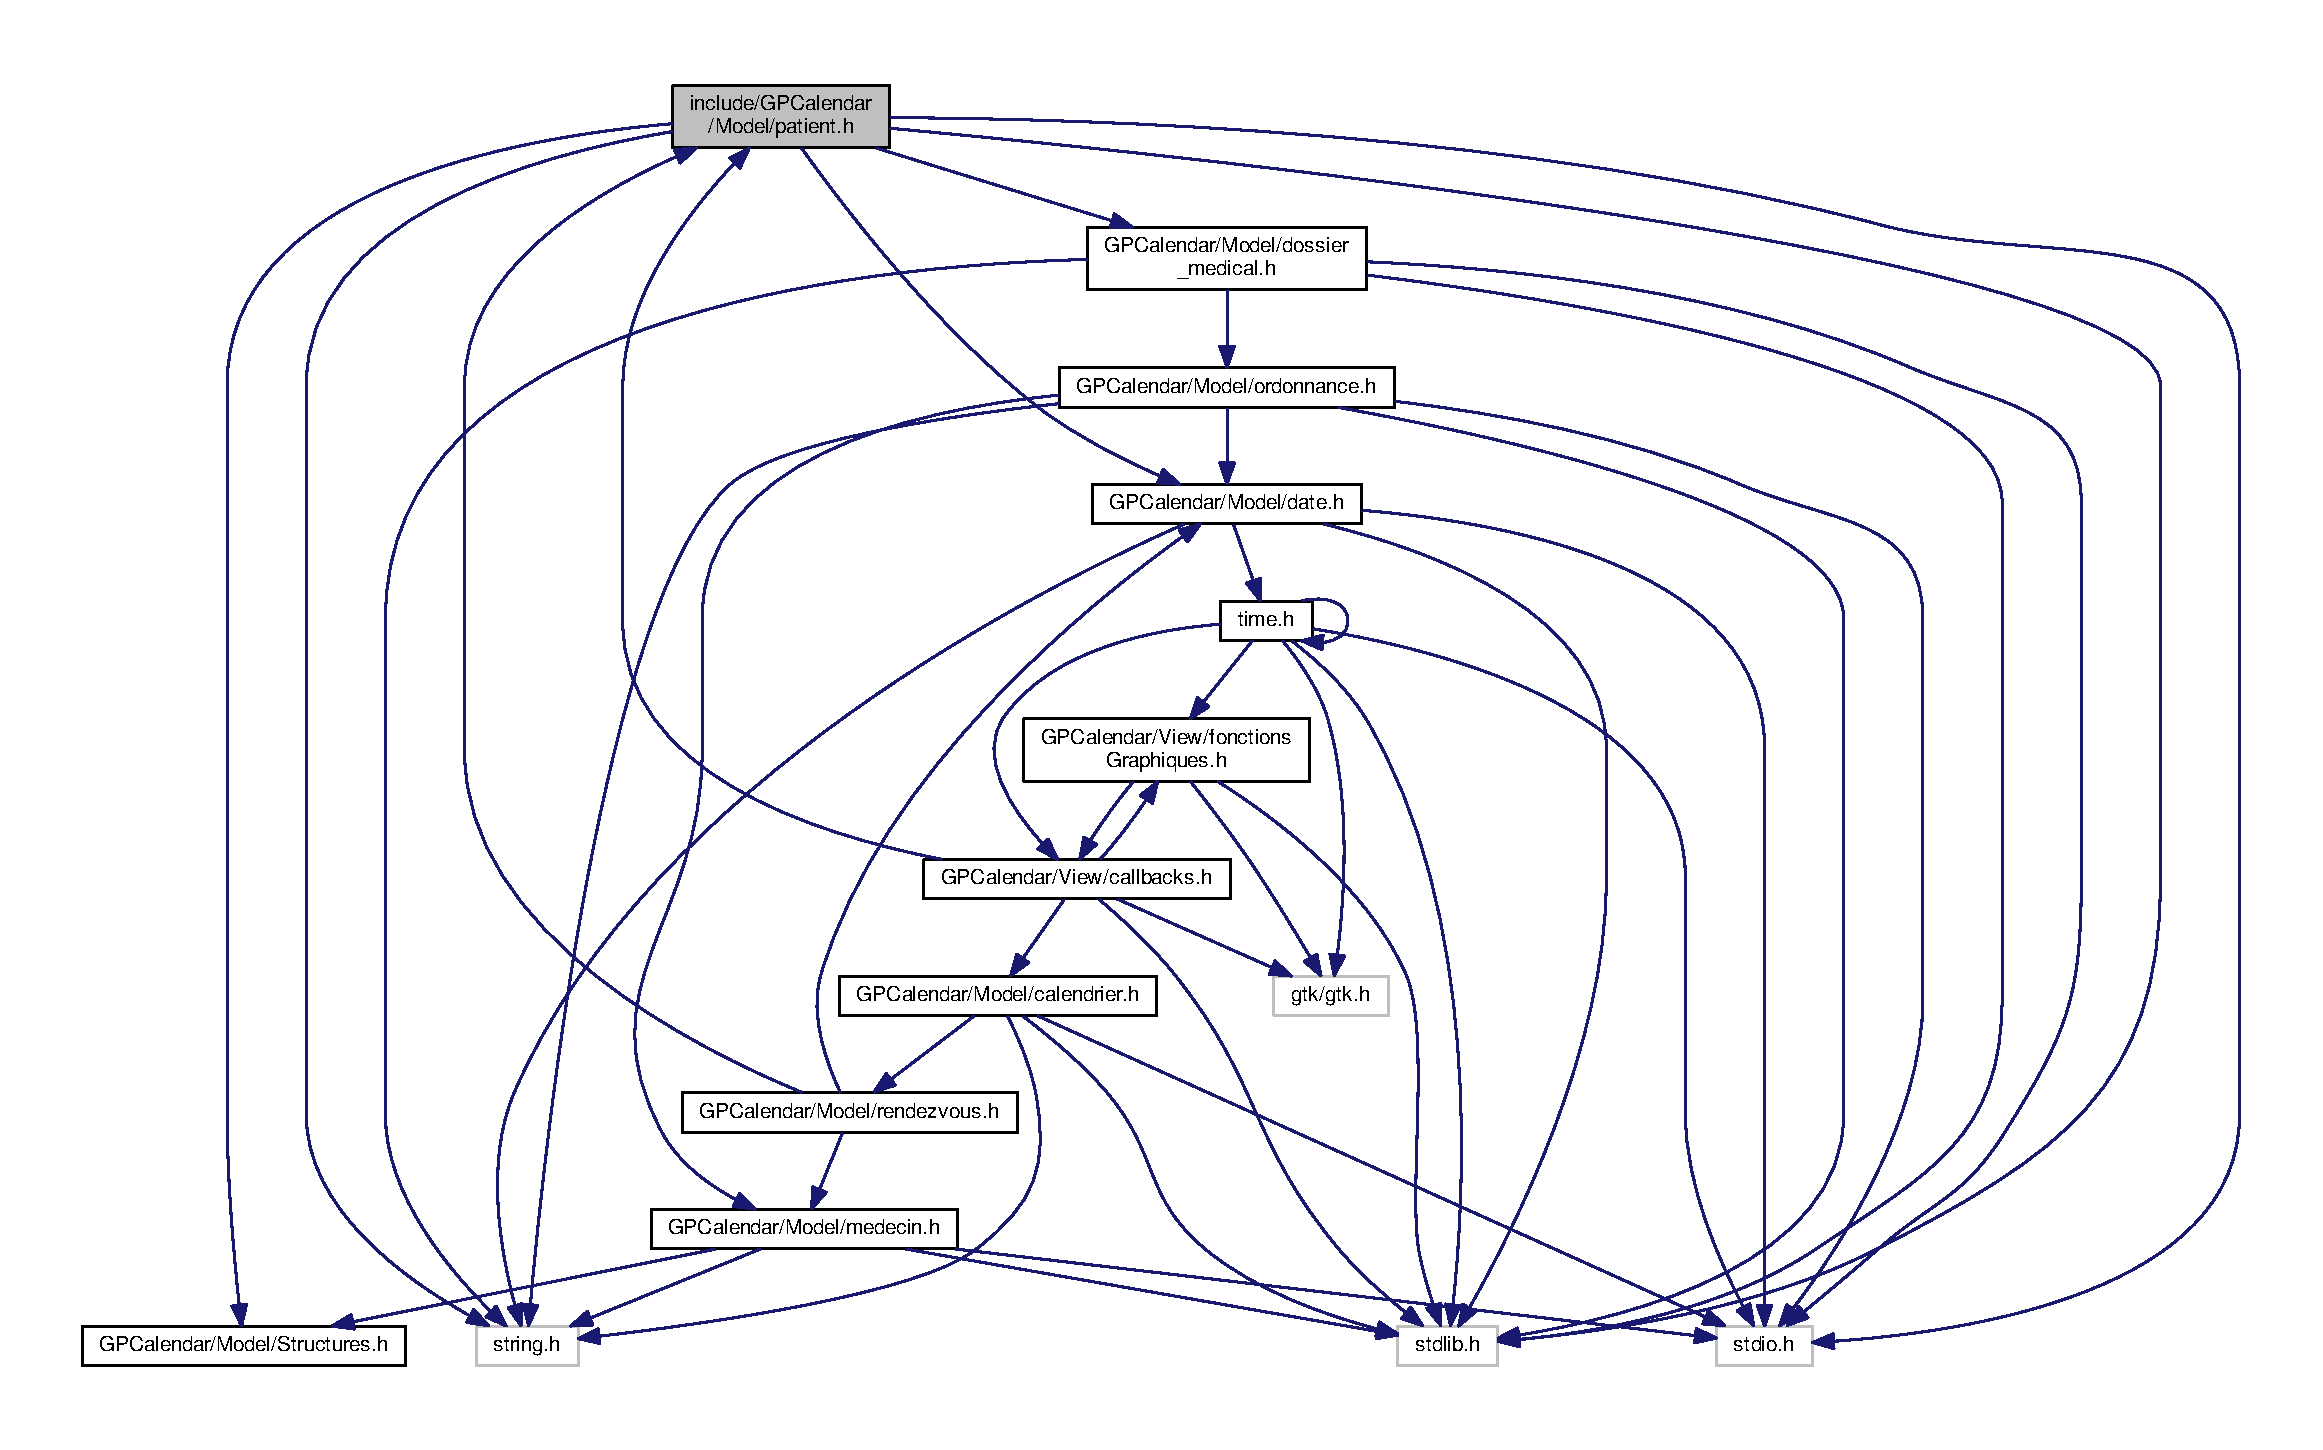
\includegraphics[width=350pt]{patient_8h__incl}
\end{center}
\end{figure}
Ce graphe montre quels fichiers incluent directement ou indirectement ce fichier \-:
\nopagebreak
\begin{figure}[H]
\begin{center}
\leavevmode
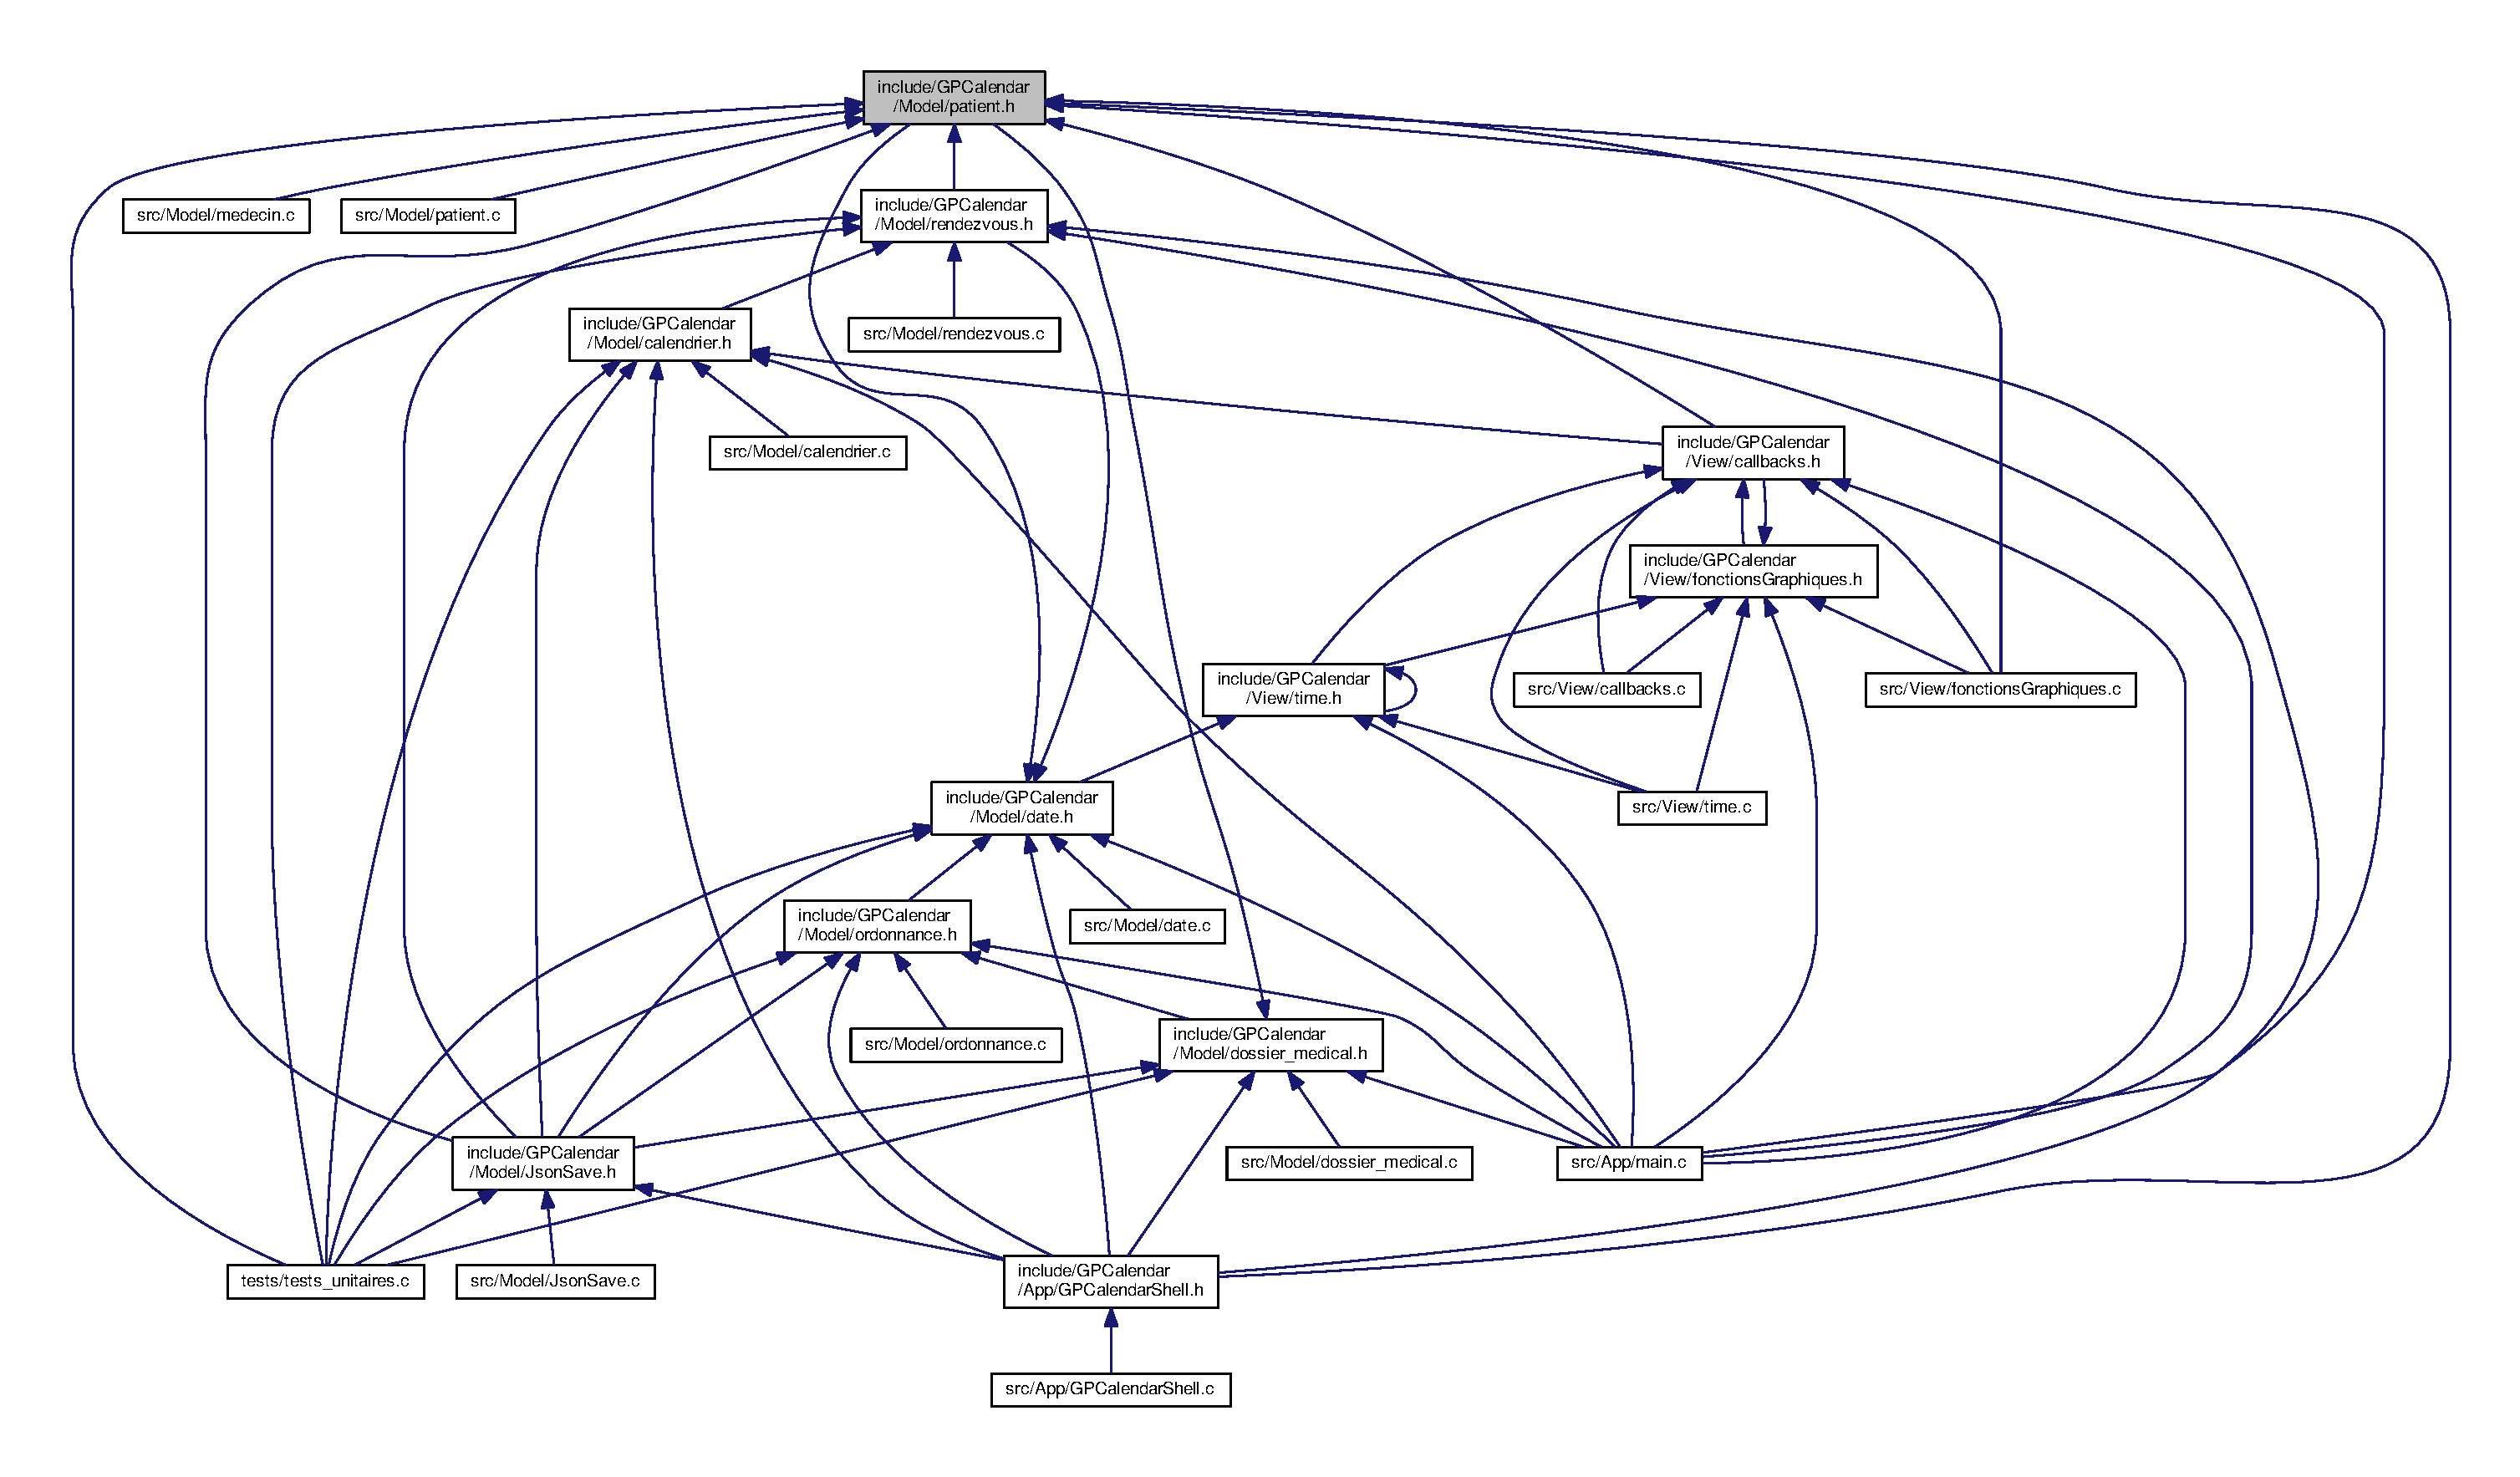
\includegraphics[width=350pt]{patient_8h__dep__incl}
\end{center}
\end{figure}
\subsection*{Structures de données}
\begin{DoxyCompactItemize}
\item 
struct \hyperlink{struct_patient}{Patient}
\item 
struct \hyperlink{struct_node_patient}{Node\-Patient}
\item 
struct \hyperlink{struct_list_patient}{List\-Patient}
\end{DoxyCompactItemize}
\subsection*{Définitions de type}
\begin{DoxyCompactItemize}
\item 
typedef struct \hyperlink{struct_node_patient}{Node\-Patient} \hyperlink{patient_8h_ab033628bfe7ba17e7160014e0b138eba}{Node\-Patient}
\end{DoxyCompactItemize}
\subsection*{Fonctions}
\begin{DoxyCompactItemize}
\item 
\hyperlink{struct_patient}{Patient} $\ast$ \hyperlink{patient_8h_a8b5d4d5e5b2e0c3238f127c8310df4d9}{Creer\-Patient} (char $\ast$nom, char $\ast$prenom, int annee\-\_\-naissance, int mois\-\_\-naissance, int jour\-\_\-naissance, char $\ast$mail, char $\ast$num\-\_\-tel, char $\ast$numero\-\_\-secu\-\_\-social)
\item 
void \hyperlink{patient_8h_a913e3a59114f7db7b7ad54f93237e7b8}{Delete\-Patient} (\hyperlink{struct_patient}{Patient} $\ast$patient)
\item 
void \hyperlink{patient_8h_a921d9b4c9ec1ea4c9db9ae6f1695041c}{print\-Patient} (char $\ast$infos, \hyperlink{struct_patient}{Patient} $\ast$p)
\item 
void \hyperlink{patient_8h_a8449a83c8157829d93cef6419dc16240}{Acces\-Dossier\-Medical} (char $\ast$infos, \hyperlink{struct_patient}{Patient} $\ast$p)
\item 
void \hyperlink{patient_8h_a910c6ac221d062e73d9847a08ada7058}{Print\-List\-Ordonnances} (char $\ast$infos, \hyperlink{struct_patient}{Patient} $\ast$p)
\item 
void \hyperlink{patient_8h_a043dbf27ffbc274d4c1cda46eb0bf979}{Print\-List\-Antecedents} (char $\ast$infos, \hyperlink{struct_patient}{Patient} $\ast$p)
\item 
void \hyperlink{patient_8h_a107931c92b5db273a4ba8a7594813560}{Set\-Nom\-Patient} (\hyperlink{struct_patient}{Patient} $\ast$p, char $\ast$nom)
\item 
void \hyperlink{patient_8h_a9b63616d2f9c0effeaa903dfb344ac51}{Set\-Prenom\-Patient} (\hyperlink{struct_patient}{Patient} $\ast$p, char $\ast$prenom)
\item 
void \hyperlink{patient_8h_a61d1c016d27141cb494c307e74b95d24}{Set\-Date\-Naissance\-Patient} (\hyperlink{struct_patient}{Patient} $\ast$p, int an, int mois, int jour)
\item 
void \hyperlink{patient_8h_a2c27261c6607f0fcf2c53fc514319829}{Set\-Adresse\-Mail\-Patient} (\hyperlink{struct_patient}{Patient} $\ast$p, char $\ast$mail)
\item 
void \hyperlink{patient_8h_a0d02d19fbbafc82e8b74ebced325d010}{Set\-Numero\-Telephone\-Patient} (\hyperlink{struct_patient}{Patient} $\ast$p, char $\ast$tel)
\item 
void \hyperlink{patient_8h_aafe2bfc75e103b3e5435e0e375d8ec79}{set\-Numero\-Secu\-Sociale\-Patient} (\hyperlink{struct_patient}{Patient} $\ast$p, char $\ast$secu)
\item 
void \hyperlink{patient_8h_a6e771e2869a7b73c4a31671c677c5d65}{get\-Nom\-Patient} (char $\ast$nom, \hyperlink{struct_patient}{Patient} $\ast$p)
\item 
void \hyperlink{patient_8h_ac149e97afc2950df9d9a0103eb44e2ae}{get\-Date\-Naissance\-Patient} (char $\ast$infos, \hyperlink{struct_patient}{Patient} $\ast$p)
\item 
char $\ast$ \hyperlink{patient_8h_abe02d8f198bbb5c6f4298b70717c68e7}{get\-Adresse\-Mail\-Patient} (\hyperlink{struct_patient}{Patient} $\ast$p)
\item 
char $\ast$ \hyperlink{patient_8h_a309b0518aa23434a7f6d73b3d8f8040c}{get\-Numero\-Telephone\-Patient} (\hyperlink{struct_patient}{Patient} $\ast$p)
\item 
char $\ast$ \hyperlink{patient_8h_a9f21fc94cc9c135c4d081949be7a65ab}{get\-Numero\-Secu\-Sociale\-Patient} (\hyperlink{struct_patient}{Patient} $\ast$p)
\item 
void \hyperlink{patient_8h_a43e60a3391b4f4e16b73e053f54ef723}{get\-Info\-Patient} (char $\ast$infos, \hyperlink{struct_patient}{Patient} $\ast$p)
\item 
int \hyperlink{patient_8h_ae44ee40bd899a1161e4c2d3e271418e5}{Add\-Medecin\-Consulte\-Patient} (\hyperlink{struct_patient}{Patient} $\ast$p, \hyperlink{struct_medecin}{Medecin} $\ast$medecin)
\item 
int \hyperlink{patient_8h_a779a417552234e4058cb0ad96356825a}{Delete\-Medecin\-Consulte\-Patient} (\hyperlink{struct_patient}{Patient} $\ast$p, \hyperlink{struct_medecin}{Medecin} $\ast$medecin)
\item 
\hyperlink{struct_node_patient}{Node\-Patient} $\ast$ \hyperlink{patient_8h_a90e466df64f56494bc1a8f2b9b3bad79}{new\-Node\-Patient} (\hyperlink{struct_patient}{Patient} $\ast$patient, \hyperlink{struct_node_patient}{Node\-Patient} $\ast$previous, \hyperlink{struct_node_patient}{Node\-Patient} $\ast$next)
\item 
void \hyperlink{patient_8h_a9a09bf67c1092dbdfa73ff1ea76fdf4f}{free\-Node\-Patient} (\hyperlink{struct_list_patient}{List\-Patient} $\ast$l, \hyperlink{struct_node_patient}{Node\-Patient} $\ast$n)
\item 
void \hyperlink{patient_8h_a6d541623f574ba0350a99d58a5bd7233}{free\-Node\-Patient\-\_\-without\-Deleting\-Patient} (\hyperlink{struct_list_patient}{List\-Patient} $\ast$l, \hyperlink{struct_node_patient}{Node\-Patient} $\ast$n)
\item 
\hyperlink{struct_list_patient}{List\-Patient} $\ast$ \hyperlink{patient_8h_abc0bc3b9a71753ea5858655b57d08fdf}{Creer\-List\-Patient} ()
\item 
void \hyperlink{patient_8h_ae4b1fb7666f84cd621dfc7bd3d11bac2}{print\-List\-Patient} (\hyperlink{struct_list_patient}{List\-Patient} $\ast$l)
\item 
void \hyperlink{patient_8h_aef369d7967f5efb44d2460bcc38f858f}{List\-Patient\-\_\-init} (\hyperlink{struct_list_patient}{List\-Patient} $\ast$l)
\item 
void \hyperlink{patient_8h_a70941926bd9e1bccd87d03f276bc19ef}{List\-Patient\-\_\-free} (\hyperlink{struct_list_patient}{List\-Patient} $\ast$l)
\item 
void \hyperlink{patient_8h_ab8259a39f2e5f810b3b06579f66bcaff}{List\-Patient\-\_\-free\-\_\-without\-Deleting\-Patient} (\hyperlink{struct_list_patient}{List\-Patient} $\ast$l)
\item 
int \hyperlink{patient_8h_ad3df2db8b2f9aa4b687953750aa74575}{List\-Patient\-\_\-add} (\hyperlink{struct_list_patient}{List\-Patient} $\ast$l, \hyperlink{struct_patient}{Patient} $\ast$p)
\item 
\hyperlink{struct_patient}{Patient} $\ast$ \hyperlink{patient_8h_a34684100f534f247f56b3690ec750840}{List\-Patient\-\_\-seek} (\hyperlink{struct_list_patient}{List\-Patient} $\ast$l\-P, char $\ast$I\-D\-Patient)
\item 
int \hyperlink{patient_8h_accdf4cb18ba0cc4d1001f3f4be49f2a2}{List\-Patient\-\_\-is\-Empty} (\hyperlink{struct_list_patient}{List\-Patient} $\ast$l)
\item 
int \hyperlink{patient_8h_af7422a8737c994810c07693b2fbc9e62}{List\-Patient\-\_\-is\-First} (\hyperlink{struct_list_patient}{List\-Patient} $\ast$l)
\item 
int \hyperlink{patient_8h_a22eee7a20d99884fc52b91d9a229eb91}{List\-Patient\-\_\-is\-Last} (\hyperlink{struct_list_patient}{List\-Patient} $\ast$l)
\item 
int \hyperlink{patient_8h_a03cd9855165013b548796ad7029fe464}{List\-Patient\-\_\-is\-Out\-Of\-List} (\hyperlink{struct_list_patient}{List\-Patient} $\ast$l)
\item 
void \hyperlink{patient_8h_ad448b7ab4a5637b55d3ce8efaf1c0f08}{List\-Patient\-\_\-set\-On\-First} (\hyperlink{struct_list_patient}{List\-Patient} $\ast$l)
\item 
void \hyperlink{patient_8h_a9c45a8273c719007d1904151c0e0b94d}{List\-Patient\-\_\-set\-On\-Last} (\hyperlink{struct_list_patient}{List\-Patient} $\ast$l)
\item 
void \hyperlink{patient_8h_a32ded12aa7f7b4110ed76530329c8293}{List\-Patient\-\_\-set\-On\-Next} (\hyperlink{struct_list_patient}{List\-Patient} $\ast$l)
\item 
void \hyperlink{patient_8h_aa695434fd4bc74a7190a12da0648af98}{List\-Patient\-\_\-set\-On\-Previous} (\hyperlink{struct_list_patient}{List\-Patient} $\ast$l)
\item 
\hyperlink{struct_patient}{Patient} $\ast$ \hyperlink{patient_8h_aa3d3c99d20cac60062f3a9a2dd2ef68f}{List\-Patient\-\_\-get\-Current} (\hyperlink{struct_list_patient}{List\-Patient} $\ast$l)
\end{DoxyCompactItemize}


\subsection{Documentation des définitions de type}
\hypertarget{patient_8h_ab033628bfe7ba17e7160014e0b138eba}{\index{patient.\-h@{patient.\-h}!Node\-Patient@{Node\-Patient}}
\index{Node\-Patient@{Node\-Patient}!patient.h@{patient.\-h}}
\subsubsection[{Node\-Patient}]{\setlength{\rightskip}{0pt plus 5cm}typedef struct {\bf Node\-Patient} {\bf Node\-Patient}}}\label{patient_8h_ab033628bfe7ba17e7160014e0b138eba}
Structure \hyperlink{struct_node_patient}{Node\-Patient} permettant de créer une Doubly linked list avec des sentinels pour la liste des Medecins consultés par un patient 

\subsection{Documentation des fonctions}
\hypertarget{patient_8h_a8449a83c8157829d93cef6419dc16240}{\index{patient.\-h@{patient.\-h}!Acces\-Dossier\-Medical@{Acces\-Dossier\-Medical}}
\index{Acces\-Dossier\-Medical@{Acces\-Dossier\-Medical}!patient.h@{patient.\-h}}
\subsubsection[{Acces\-Dossier\-Medical}]{\setlength{\rightskip}{0pt plus 5cm}void Acces\-Dossier\-Medical (
\begin{DoxyParamCaption}
\item[{char $\ast$}]{infos, }
\item[{{\bf Patient} $\ast$}]{p}
\end{DoxyParamCaption}
)}}\label{patient_8h_a8449a83c8157829d93cef6419dc16240}
Acces\-Dossier\-Medical \-: Accede au dossier du patient et l'affiche 
\begin{DoxyParams}{Paramètres}
{\em p} & \-: le patient dont on veut acceder au dossier \\
\hline
\end{DoxyParams}
\hypertarget{patient_8h_ae44ee40bd899a1161e4c2d3e271418e5}{\index{patient.\-h@{patient.\-h}!Add\-Medecin\-Consulte\-Patient@{Add\-Medecin\-Consulte\-Patient}}
\index{Add\-Medecin\-Consulte\-Patient@{Add\-Medecin\-Consulte\-Patient}!patient.h@{patient.\-h}}
\subsubsection[{Add\-Medecin\-Consulte\-Patient}]{\setlength{\rightskip}{0pt plus 5cm}int Add\-Medecin\-Consulte\-Patient (
\begin{DoxyParamCaption}
\item[{{\bf Patient} $\ast$}]{p, }
\item[{{\bf Medecin} $\ast$}]{medecin}
\end{DoxyParamCaption}
)}}\label{patient_8h_ae44ee40bd899a1161e4c2d3e271418e5}
Add\-Medecinc\-Consulte\-Patient \-: Ajoute un \hyperlink{struct_medecin}{Medecin} à la première position de la liste des medecins consultés par un patient 
\begin{DoxyParams}{Paramètres}
{\em p} & \-: le patient consultant \\
\hline
{\em medecin} & \-: le medecin consulté \\
\hline
\end{DoxyParams}
\begin{DoxyReturn}{Renvoie}
1 si le médecin a bien été ajouté à la liste 0 sinon (médecin déjà consulté par exemple) 
\end{DoxyReturn}
\hypertarget{patient_8h_abc0bc3b9a71753ea5858655b57d08fdf}{\index{patient.\-h@{patient.\-h}!Creer\-List\-Patient@{Creer\-List\-Patient}}
\index{Creer\-List\-Patient@{Creer\-List\-Patient}!patient.h@{patient.\-h}}
\subsubsection[{Creer\-List\-Patient}]{\setlength{\rightskip}{0pt plus 5cm}{\bf List\-Patient}$\ast$ Creer\-List\-Patient (
\begin{DoxyParamCaption}
{}
\end{DoxyParamCaption}
)}}\label{patient_8h_abc0bc3b9a71753ea5858655b57d08fdf}
Creer\-List\-Patient \-: malloc et initialise une liste de patients \begin{DoxyReturn}{Renvoie}
la liste initialisée 
\end{DoxyReturn}
\hypertarget{patient_8h_a8b5d4d5e5b2e0c3238f127c8310df4d9}{\index{patient.\-h@{patient.\-h}!Creer\-Patient@{Creer\-Patient}}
\index{Creer\-Patient@{Creer\-Patient}!patient.h@{patient.\-h}}
\subsubsection[{Creer\-Patient}]{\setlength{\rightskip}{0pt plus 5cm}{\bf Patient}$\ast$ Creer\-Patient (
\begin{DoxyParamCaption}
\item[{char $\ast$}]{nom, }
\item[{char $\ast$}]{prenom, }
\item[{int}]{annee\-\_\-naissance, }
\item[{int}]{mois\-\_\-naissance, }
\item[{int}]{jour\-\_\-naissance, }
\item[{char $\ast$}]{mail, }
\item[{char $\ast$}]{num\-\_\-tel, }
\item[{char $\ast$}]{numero\-\_\-secu\-\_\-social}
\end{DoxyParamCaption}
)}}\label{patient_8h_a8b5d4d5e5b2e0c3238f127c8310df4d9}
Creer\-Patient \-: Creer une nouvelle instance de la structure \hyperlink{struct_patient}{Patient} avec toutes les informations basiques 
\begin{DoxyParams}{Paramètres}
{\em nom} & \-: nom du patient \\
\hline
{\em prenom} & \-: prénom du patient \\
\hline
{\em annee\-\_\-naissance} & \-: Année, mois et jour de naissance du patient \\
\hline
{\em mois\-\_\-naissance} & \\
\hline
{\em jour\-\_\-naissance} & \\
\hline
{\em mail} & \-: adresse mail du patient \\
\hline
{\em num\-\_\-tel} & \-:numéro de téléphone du patient \\
\hline
\end{DoxyParams}
\begin{DoxyReturn}{Renvoie}
un pointeur sur le patient créé 
\end{DoxyReturn}
\hypertarget{patient_8h_a779a417552234e4058cb0ad96356825a}{\index{patient.\-h@{patient.\-h}!Delete\-Medecin\-Consulte\-Patient@{Delete\-Medecin\-Consulte\-Patient}}
\index{Delete\-Medecin\-Consulte\-Patient@{Delete\-Medecin\-Consulte\-Patient}!patient.h@{patient.\-h}}
\subsubsection[{Delete\-Medecin\-Consulte\-Patient}]{\setlength{\rightskip}{0pt plus 5cm}int Delete\-Medecin\-Consulte\-Patient (
\begin{DoxyParamCaption}
\item[{{\bf Patient} $\ast$}]{p, }
\item[{{\bf Medecin} $\ast$}]{medecin}
\end{DoxyParamCaption}
)}}\label{patient_8h_a779a417552234e4058cb0ad96356825a}
Delete\-Medecin\-Patient \-: Enleve un \hyperlink{struct_medecin}{Medecin} de la liste des medecins consultés par un patient 
\begin{DoxyParams}{Paramètres}
{\em p} & \-: le patient à qui on retire un medecin consultés \\
\hline
{\em medecin} & \-: le medecin qui n'a pas été consulté \\
\hline
\end{DoxyParams}
\begin{DoxyReturn}{Renvoie}
1 si l'enlevement du médecin a bien été réalisé 0 sinon (le patient n'avait pas consulté ce médecin par exemple) 
\end{DoxyReturn}
\hypertarget{patient_8h_a913e3a59114f7db7b7ad54f93237e7b8}{\index{patient.\-h@{patient.\-h}!Delete\-Patient@{Delete\-Patient}}
\index{Delete\-Patient@{Delete\-Patient}!patient.h@{patient.\-h}}
\subsubsection[{Delete\-Patient}]{\setlength{\rightskip}{0pt plus 5cm}void Delete\-Patient (
\begin{DoxyParamCaption}
\item[{{\bf Patient} $\ast$}]{patient}
\end{DoxyParamCaption}
)}}\label{patient_8h_a913e3a59114f7db7b7ad54f93237e7b8}
Delete\-Patient \-: Supprime proprement une instance de la structure patient 
\begin{DoxyParams}{Paramètres}
{\em patient} & \-: le patient à supprimer \\
\hline
\end{DoxyParams}
\hypertarget{patient_8h_a9a09bf67c1092dbdfa73ff1ea76fdf4f}{\index{patient.\-h@{patient.\-h}!free\-Node\-Patient@{free\-Node\-Patient}}
\index{free\-Node\-Patient@{free\-Node\-Patient}!patient.h@{patient.\-h}}
\subsubsection[{free\-Node\-Patient}]{\setlength{\rightskip}{0pt plus 5cm}void free\-Node\-Patient (
\begin{DoxyParamCaption}
\item[{{\bf List\-Patient} $\ast$}]{l, }
\item[{{\bf Node\-Patient} $\ast$}]{n}
\end{DoxyParamCaption}
)}}\label{patient_8h_a9a09bf67c1092dbdfa73ff1ea76fdf4f}
free\-Node\-Patient \-: Permet de delete proprement (avec un free) un node\-Patient 
\begin{DoxyParams}{Paramètres}
{\em n} & \-: le node à delete \\
\hline
\end{DoxyParams}
\hypertarget{patient_8h_a6d541623f574ba0350a99d58a5bd7233}{\index{patient.\-h@{patient.\-h}!free\-Node\-Patient\-\_\-without\-Deleting\-Patient@{free\-Node\-Patient\-\_\-without\-Deleting\-Patient}}
\index{free\-Node\-Patient\-\_\-without\-Deleting\-Patient@{free\-Node\-Patient\-\_\-without\-Deleting\-Patient}!patient.h@{patient.\-h}}
\subsubsection[{free\-Node\-Patient\-\_\-without\-Deleting\-Patient}]{\setlength{\rightskip}{0pt plus 5cm}void free\-Node\-Patient\-\_\-without\-Deleting\-Patient (
\begin{DoxyParamCaption}
\item[{{\bf List\-Patient} $\ast$}]{l, }
\item[{{\bf Node\-Patient} $\ast$}]{n}
\end{DoxyParamCaption}
)}}\label{patient_8h_a6d541623f574ba0350a99d58a5bd7233}
free\-Node\-Patient\-\_\-without\-Deleting\-Patient \-: Permet de delete proprement (avec un free) un node\-Patient 
\begin{DoxyParams}{Paramètres}
{\em n} & \-: le node à delete \\
\hline
\end{DoxyParams}
\hypertarget{patient_8h_abe02d8f198bbb5c6f4298b70717c68e7}{\index{patient.\-h@{patient.\-h}!get\-Adresse\-Mail\-Patient@{get\-Adresse\-Mail\-Patient}}
\index{get\-Adresse\-Mail\-Patient@{get\-Adresse\-Mail\-Patient}!patient.h@{patient.\-h}}
\subsubsection[{get\-Adresse\-Mail\-Patient}]{\setlength{\rightskip}{0pt plus 5cm}char$\ast$ get\-Adresse\-Mail\-Patient (
\begin{DoxyParamCaption}
\item[{{\bf Patient} $\ast$}]{p}
\end{DoxyParamCaption}
)}}\label{patient_8h_abe02d8f198bbb5c6f4298b70717c68e7}
get\-Adresse\-Mail\-Patient \-: retourne l'adresse mail du patient sous forme de char$\ast$ (pour l'affichage) 
\begin{DoxyParams}{Paramètres}
{\em p} & \-: le patient dont on veut l'adresse mail \\
\hline
\end{DoxyParams}
\begin{DoxyReturn}{Renvoie}
un char$\ast$ avec l'dresse mail 
\end{DoxyReturn}
\hypertarget{patient_8h_ac149e97afc2950df9d9a0103eb44e2ae}{\index{patient.\-h@{patient.\-h}!get\-Date\-Naissance\-Patient@{get\-Date\-Naissance\-Patient}}
\index{get\-Date\-Naissance\-Patient@{get\-Date\-Naissance\-Patient}!patient.h@{patient.\-h}}
\subsubsection[{get\-Date\-Naissance\-Patient}]{\setlength{\rightskip}{0pt plus 5cm}void get\-Date\-Naissance\-Patient (
\begin{DoxyParamCaption}
\item[{char $\ast$}]{infos, }
\item[{{\bf Patient} $\ast$}]{p}
\end{DoxyParamCaption}
)}}\label{patient_8h_ac149e97afc2950df9d9a0103eb44e2ae}
get\-Date\-Naissance\-Patient \-: met la date de naissance du patient sous forme de char$\ast$ (pour l'affichage) dans infos 
\begin{DoxyParams}{Paramètres}
{\em infos} & \-: le char$\ast$ dans lequel on stocke la date \\
\hline
{\em p} & \-: le patient dont on veut la date de naissance \\
\hline
\end{DoxyParams}
\hypertarget{patient_8h_a43e60a3391b4f4e16b73e053f54ef723}{\index{patient.\-h@{patient.\-h}!get\-Info\-Patient@{get\-Info\-Patient}}
\index{get\-Info\-Patient@{get\-Info\-Patient}!patient.h@{patient.\-h}}
\subsubsection[{get\-Info\-Patient}]{\setlength{\rightskip}{0pt plus 5cm}void get\-Info\-Patient (
\begin{DoxyParamCaption}
\item[{char $\ast$}]{infos, }
\item[{{\bf Patient} $\ast$}]{p}
\end{DoxyParamCaption}
)}}\label{patient_8h_a43e60a3391b4f4e16b73e053f54ef723}
get\-Info\-Patient \-: Place les infos du patient dans infos 
\begin{DoxyParams}{Paramètres}
{\em infos} & \-: le char$\ast$ dans lequel on met les infos \\
\hline
{\em p} & \-: le patient dont on veut les informations \\
\hline
\end{DoxyParams}
\hypertarget{patient_8h_a6e771e2869a7b73c4a31671c677c5d65}{\index{patient.\-h@{patient.\-h}!get\-Nom\-Patient@{get\-Nom\-Patient}}
\index{get\-Nom\-Patient@{get\-Nom\-Patient}!patient.h@{patient.\-h}}
\subsubsection[{get\-Nom\-Patient}]{\setlength{\rightskip}{0pt plus 5cm}void get\-Nom\-Patient (
\begin{DoxyParamCaption}
\item[{char $\ast$}]{nom, }
\item[{{\bf Patient} $\ast$}]{p}
\end{DoxyParamCaption}
)}}\label{patient_8h_a6e771e2869a7b73c4a31671c677c5d65}
get\-Nom\-Patient \-: retourne le nom et le prénom du patient sous forme de char$\ast$ (pour l'affichage du R\-D\-V) 
\begin{DoxyParams}{Paramètres}
{\em p} & \-: le patient dont on veut le nom \\
\hline
\end{DoxyParams}
\begin{DoxyReturn}{Renvoie}
une chaine de caractères avec le nom et le prénom du patient 
\end{DoxyReturn}
\hypertarget{patient_8h_a9f21fc94cc9c135c4d081949be7a65ab}{\index{patient.\-h@{patient.\-h}!get\-Numero\-Secu\-Sociale\-Patient@{get\-Numero\-Secu\-Sociale\-Patient}}
\index{get\-Numero\-Secu\-Sociale\-Patient@{get\-Numero\-Secu\-Sociale\-Patient}!patient.h@{patient.\-h}}
\subsubsection[{get\-Numero\-Secu\-Sociale\-Patient}]{\setlength{\rightskip}{0pt plus 5cm}char$\ast$ get\-Numero\-Secu\-Sociale\-Patient (
\begin{DoxyParamCaption}
\item[{{\bf Patient} $\ast$}]{p}
\end{DoxyParamCaption}
)}}\label{patient_8h_a9f21fc94cc9c135c4d081949be7a65ab}
get\-Numero\-Secu\-Sociale\-Patient \-: retourne le numéro de sécurité sociale du patient sous forme de char$\ast$ (pour l'affichage) 
\begin{DoxyParams}{Paramètres}
{\em p} & \-: le patient dont on veut le numéro de sécurité sociale \\
\hline
\end{DoxyParams}
\begin{DoxyReturn}{Renvoie}
un char $\ast$ avec le numero de sécurité sociale 
\end{DoxyReturn}
\hypertarget{patient_8h_a309b0518aa23434a7f6d73b3d8f8040c}{\index{patient.\-h@{patient.\-h}!get\-Numero\-Telephone\-Patient@{get\-Numero\-Telephone\-Patient}}
\index{get\-Numero\-Telephone\-Patient@{get\-Numero\-Telephone\-Patient}!patient.h@{patient.\-h}}
\subsubsection[{get\-Numero\-Telephone\-Patient}]{\setlength{\rightskip}{0pt plus 5cm}char$\ast$ get\-Numero\-Telephone\-Patient (
\begin{DoxyParamCaption}
\item[{{\bf Patient} $\ast$}]{p}
\end{DoxyParamCaption}
)}}\label{patient_8h_a309b0518aa23434a7f6d73b3d8f8040c}
get\-Numero\-Telephone\-Patient \-: retourne le numéro de téléphone du patient sous forme de char$\ast$ (pour l'affichage) 
\begin{DoxyParams}{Paramètres}
{\em p} & \-: le patient dont on veut le numéro de téléphone \\
\hline
\end{DoxyParams}
\begin{DoxyReturn}{Renvoie}
un char $\ast$ avec le numero de téléphone 
\end{DoxyReturn}
\hypertarget{patient_8h_ad3df2db8b2f9aa4b687953750aa74575}{\index{patient.\-h@{patient.\-h}!List\-Patient\-\_\-add@{List\-Patient\-\_\-add}}
\index{List\-Patient\-\_\-add@{List\-Patient\-\_\-add}!patient.h@{patient.\-h}}
\subsubsection[{List\-Patient\-\_\-add}]{\setlength{\rightskip}{0pt plus 5cm}int List\-Patient\-\_\-add (
\begin{DoxyParamCaption}
\item[{{\bf List\-Patient} $\ast$}]{l, }
\item[{{\bf Patient} $\ast$}]{p}
\end{DoxyParamCaption}
)}}\label{patient_8h_ad3df2db8b2f9aa4b687953750aa74575}
List\-Patient\-\_\-add \-: Ajoute un patient à une liste de patients (pas triée) 
\begin{DoxyParams}{Paramètres}
{\em l} & \-: la liste à laquelle on ajoute \\
\hline
{\em p} & \-: le patient à ajouter \\
\hline
\end{DoxyParams}
\begin{DoxyReturn}{Renvoie}
-\/1 si la liste ou le patient étaient N\-U\-L\-L 1 si tout s'est bien passé 
\end{DoxyReturn}
\hypertarget{patient_8h_a70941926bd9e1bccd87d03f276bc19ef}{\index{patient.\-h@{patient.\-h}!List\-Patient\-\_\-free@{List\-Patient\-\_\-free}}
\index{List\-Patient\-\_\-free@{List\-Patient\-\_\-free}!patient.h@{patient.\-h}}
\subsubsection[{List\-Patient\-\_\-free}]{\setlength{\rightskip}{0pt plus 5cm}void List\-Patient\-\_\-free (
\begin{DoxyParamCaption}
\item[{{\bf List\-Patient} $\ast$}]{l}
\end{DoxyParamCaption}
)}}\label{patient_8h_a70941926bd9e1bccd87d03f276bc19ef}
List\-Patient\-\_\-free \-: Free toute la liste de patients 
\begin{DoxyParams}{Paramètres}
{\em l} & \-: la liste en question \\
\hline
\end{DoxyParams}
\hypertarget{patient_8h_ab8259a39f2e5f810b3b06579f66bcaff}{\index{patient.\-h@{patient.\-h}!List\-Patient\-\_\-free\-\_\-without\-Deleting\-Patient@{List\-Patient\-\_\-free\-\_\-without\-Deleting\-Patient}}
\index{List\-Patient\-\_\-free\-\_\-without\-Deleting\-Patient@{List\-Patient\-\_\-free\-\_\-without\-Deleting\-Patient}!patient.h@{patient.\-h}}
\subsubsection[{List\-Patient\-\_\-free\-\_\-without\-Deleting\-Patient}]{\setlength{\rightskip}{0pt plus 5cm}void List\-Patient\-\_\-free\-\_\-without\-Deleting\-Patient (
\begin{DoxyParamCaption}
\item[{{\bf List\-Patient} $\ast$}]{l}
\end{DoxyParamCaption}
)}}\label{patient_8h_ab8259a39f2e5f810b3b06579f66bcaff}
List\-Patient\-\_\-free\-\_\-without\-Deleting\-Patient \-: Free toute la liste de patients 
\begin{DoxyParams}{Paramètres}
{\em l} & \-: la liste en question \\
\hline
\end{DoxyParams}
\hypertarget{patient_8h_aa3d3c99d20cac60062f3a9a2dd2ef68f}{\index{patient.\-h@{patient.\-h}!List\-Patient\-\_\-get\-Current@{List\-Patient\-\_\-get\-Current}}
\index{List\-Patient\-\_\-get\-Current@{List\-Patient\-\_\-get\-Current}!patient.h@{patient.\-h}}
\subsubsection[{List\-Patient\-\_\-get\-Current}]{\setlength{\rightskip}{0pt plus 5cm}{\bf Patient}$\ast$ List\-Patient\-\_\-get\-Current (
\begin{DoxyParamCaption}
\item[{{\bf List\-Patient} $\ast$}]{l}
\end{DoxyParamCaption}
)}}\label{patient_8h_aa3d3c99d20cac60062f3a9a2dd2ef68f}
List\-Patient\-\_\-get\-Current \-: Permet d'acceder au \hyperlink{struct_patient}{Patient} pointé par current 
\begin{DoxyParams}{Paramètres}
{\em l} & \-: la liste \\
\hline
\end{DoxyParams}
\begin{DoxyReturn}{Renvoie}
Retourne un pointeur sur le \hyperlink{struct_patient}{Patient} de l'élément courant de la liste 
\end{DoxyReturn}
\hypertarget{patient_8h_aef369d7967f5efb44d2460bcc38f858f}{\index{patient.\-h@{patient.\-h}!List\-Patient\-\_\-init@{List\-Patient\-\_\-init}}
\index{List\-Patient\-\_\-init@{List\-Patient\-\_\-init}!patient.h@{patient.\-h}}
\subsubsection[{List\-Patient\-\_\-init}]{\setlength{\rightskip}{0pt plus 5cm}void List\-Patient\-\_\-init (
\begin{DoxyParamCaption}
\item[{{\bf List\-Patient} $\ast$}]{l}
\end{DoxyParamCaption}
)}}\label{patient_8h_aef369d7967f5efb44d2460bcc38f858f}
List\-Patient\-\_\-init \-: Initialise correctement une liste de \hyperlink{struct_node_patient}{Node\-Patient} en reliant sentinel\-\_\-begin et end entre eux et en mettant current à N\-U\-L\-L en dehors de la liste 
\begin{DoxyParams}{Paramètres}
{\em l} & \-: la liste à initialiser \\
\hline
\end{DoxyParams}
\hypertarget{patient_8h_accdf4cb18ba0cc4d1001f3f4be49f2a2}{\index{patient.\-h@{patient.\-h}!List\-Patient\-\_\-is\-Empty@{List\-Patient\-\_\-is\-Empty}}
\index{List\-Patient\-\_\-is\-Empty@{List\-Patient\-\_\-is\-Empty}!patient.h@{patient.\-h}}
\subsubsection[{List\-Patient\-\_\-is\-Empty}]{\setlength{\rightskip}{0pt plus 5cm}int List\-Patient\-\_\-is\-Empty (
\begin{DoxyParamCaption}
\item[{{\bf List\-Patient} $\ast$}]{l}
\end{DoxyParamCaption}
)}}\label{patient_8h_accdf4cb18ba0cc4d1001f3f4be49f2a2}
List\-Patient\-\_\-is\-Empty \-: Vérifie si la liste de \hyperlink{struct_patient}{Patient} est vide ou non 
\begin{DoxyParams}{Paramètres}
{\em l} & \-: la liste \\
\hline
\end{DoxyParams}
\begin{DoxyReturn}{Renvoie}
1 si la liste est vide 0 si elle ne l'est pas -\/1 si la liste est N\-U\-L\-L 
\end{DoxyReturn}
\hypertarget{patient_8h_af7422a8737c994810c07693b2fbc9e62}{\index{patient.\-h@{patient.\-h}!List\-Patient\-\_\-is\-First@{List\-Patient\-\_\-is\-First}}
\index{List\-Patient\-\_\-is\-First@{List\-Patient\-\_\-is\-First}!patient.h@{patient.\-h}}
\subsubsection[{List\-Patient\-\_\-is\-First}]{\setlength{\rightskip}{0pt plus 5cm}int List\-Patient\-\_\-is\-First (
\begin{DoxyParamCaption}
\item[{{\bf List\-Patient} $\ast$}]{l}
\end{DoxyParamCaption}
)}}\label{patient_8h_af7422a8737c994810c07693b2fbc9e62}
List\-Patient\-\_\-is\-First \-: Vérifie si current est positionné sur le premier élément de la liste 
\begin{DoxyParams}{Paramètres}
{\em l} & \-: la liste \\
\hline
\end{DoxyParams}
\begin{DoxyReturn}{Renvoie}
1 si current est bien sur le premier élément 0 si il ne l'est pas -\/1 si la liste est N\-U\-L\-L 
\end{DoxyReturn}
\hypertarget{patient_8h_a22eee7a20d99884fc52b91d9a229eb91}{\index{patient.\-h@{patient.\-h}!List\-Patient\-\_\-is\-Last@{List\-Patient\-\_\-is\-Last}}
\index{List\-Patient\-\_\-is\-Last@{List\-Patient\-\_\-is\-Last}!patient.h@{patient.\-h}}
\subsubsection[{List\-Patient\-\_\-is\-Last}]{\setlength{\rightskip}{0pt plus 5cm}int List\-Patient\-\_\-is\-Last (
\begin{DoxyParamCaption}
\item[{{\bf List\-Patient} $\ast$}]{l}
\end{DoxyParamCaption}
)}}\label{patient_8h_a22eee7a20d99884fc52b91d9a229eb91}
List\-Patient\-\_\-is\-Last \-: Vérifie si current est positionné sur le dernier élément de la liste 
\begin{DoxyParams}{Paramètres}
{\em l} & \-: la liste \\
\hline
\end{DoxyParams}
\begin{DoxyReturn}{Renvoie}
1 si current est bien sur le dernier élément 0 si il ne l'est pas -\/1 si la liste est N\-U\-L\-L 
\end{DoxyReturn}
\hypertarget{patient_8h_a03cd9855165013b548796ad7029fe464}{\index{patient.\-h@{patient.\-h}!List\-Patient\-\_\-is\-Out\-Of\-List@{List\-Patient\-\_\-is\-Out\-Of\-List}}
\index{List\-Patient\-\_\-is\-Out\-Of\-List@{List\-Patient\-\_\-is\-Out\-Of\-List}!patient.h@{patient.\-h}}
\subsubsection[{List\-Patient\-\_\-is\-Out\-Of\-List}]{\setlength{\rightskip}{0pt plus 5cm}int List\-Patient\-\_\-is\-Out\-Of\-List (
\begin{DoxyParamCaption}
\item[{{\bf List\-Patient} $\ast$}]{l}
\end{DoxyParamCaption}
)}}\label{patient_8h_a03cd9855165013b548796ad7029fe464}
List\-Patient\-\_\-is\-Out\-Of\-List \-: Vérifie si current est bien placé sur un élément de la liste 
\begin{DoxyParams}{Paramètres}
{\em l} & \-: la liste \\
\hline
\end{DoxyParams}
\begin{DoxyReturn}{Renvoie}
1 si current vaut N\-U\-L\-L 0 si il ne l'est pas -\/1 si la liste est N\-U\-L\-L 
\end{DoxyReturn}
\hypertarget{patient_8h_a34684100f534f247f56b3690ec750840}{\index{patient.\-h@{patient.\-h}!List\-Patient\-\_\-seek@{List\-Patient\-\_\-seek}}
\index{List\-Patient\-\_\-seek@{List\-Patient\-\_\-seek}!patient.h@{patient.\-h}}
\subsubsection[{List\-Patient\-\_\-seek}]{\setlength{\rightskip}{0pt plus 5cm}{\bf Patient}$\ast$ List\-Patient\-\_\-seek (
\begin{DoxyParamCaption}
\item[{{\bf List\-Patient} $\ast$}]{l\-P, }
\item[{char $\ast$}]{I\-D\-Patient}
\end{DoxyParamCaption}
)}}\label{patient_8h_a34684100f534f247f56b3690ec750840}
Listpatient\-\_\-seek \-: Permet de chercher un patient dans une list de patient depuis son Numéro de sécurité sociale (son I\-D) 
\begin{DoxyParams}{Paramètres}
{\em l\-P} & \-: la liste dans laquelle on cherche \\
\hline
{\em I\-D\-Patient} & \-: l'I\-D du patient cherché \\
\hline
\end{DoxyParams}
\begin{DoxyReturn}{Renvoie}
un pointeur sur le patient N\-U\-L\-L si on ne l'a pas trouvé 
\end{DoxyReturn}
\hypertarget{patient_8h_ad448b7ab4a5637b55d3ce8efaf1c0f08}{\index{patient.\-h@{patient.\-h}!List\-Patient\-\_\-set\-On\-First@{List\-Patient\-\_\-set\-On\-First}}
\index{List\-Patient\-\_\-set\-On\-First@{List\-Patient\-\_\-set\-On\-First}!patient.h@{patient.\-h}}
\subsubsection[{List\-Patient\-\_\-set\-On\-First}]{\setlength{\rightskip}{0pt plus 5cm}void List\-Patient\-\_\-set\-On\-First (
\begin{DoxyParamCaption}
\item[{{\bf List\-Patient} $\ast$}]{l}
\end{DoxyParamCaption}
)}}\label{patient_8h_ad448b7ab4a5637b55d3ce8efaf1c0f08}
List\-Patient\-\_\-set\-On\-First \-: Positionne le pointeur courant sur le premier élément de la liste 
\begin{DoxyParams}{Paramètres}
{\em l} & \-: la liste \\
\hline
\end{DoxyParams}
\hypertarget{patient_8h_a9c45a8273c719007d1904151c0e0b94d}{\index{patient.\-h@{patient.\-h}!List\-Patient\-\_\-set\-On\-Last@{List\-Patient\-\_\-set\-On\-Last}}
\index{List\-Patient\-\_\-set\-On\-Last@{List\-Patient\-\_\-set\-On\-Last}!patient.h@{patient.\-h}}
\subsubsection[{List\-Patient\-\_\-set\-On\-Last}]{\setlength{\rightskip}{0pt plus 5cm}void List\-Patient\-\_\-set\-On\-Last (
\begin{DoxyParamCaption}
\item[{{\bf List\-Patient} $\ast$}]{l}
\end{DoxyParamCaption}
)}}\label{patient_8h_a9c45a8273c719007d1904151c0e0b94d}
List\-Patient\-\_\-set\-On\-Last \-: Positionne le pointeur courant sur le dernier élément de la liste 
\begin{DoxyParams}{Paramètres}
{\em l} & \-: la liste \\
\hline
\end{DoxyParams}
\hypertarget{patient_8h_a32ded12aa7f7b4110ed76530329c8293}{\index{patient.\-h@{patient.\-h}!List\-Patient\-\_\-set\-On\-Next@{List\-Patient\-\_\-set\-On\-Next}}
\index{List\-Patient\-\_\-set\-On\-Next@{List\-Patient\-\_\-set\-On\-Next}!patient.h@{patient.\-h}}
\subsubsection[{List\-Patient\-\_\-set\-On\-Next}]{\setlength{\rightskip}{0pt plus 5cm}void List\-Patient\-\_\-set\-On\-Next (
\begin{DoxyParamCaption}
\item[{{\bf List\-Patient} $\ast$}]{l}
\end{DoxyParamCaption}
)}}\label{patient_8h_a32ded12aa7f7b4110ed76530329c8293}
List\-Patient\-\_\-set\-On\-Next \-: Positionne le pointeur courant sur le prochain élément de la liste 
\begin{DoxyParams}{Paramètres}
{\em l} & \-: la liste \\
\hline
\end{DoxyParams}
\hypertarget{patient_8h_aa695434fd4bc74a7190a12da0648af98}{\index{patient.\-h@{patient.\-h}!List\-Patient\-\_\-set\-On\-Previous@{List\-Patient\-\_\-set\-On\-Previous}}
\index{List\-Patient\-\_\-set\-On\-Previous@{List\-Patient\-\_\-set\-On\-Previous}!patient.h@{patient.\-h}}
\subsubsection[{List\-Patient\-\_\-set\-On\-Previous}]{\setlength{\rightskip}{0pt plus 5cm}void List\-Patient\-\_\-set\-On\-Previous (
\begin{DoxyParamCaption}
\item[{{\bf List\-Patient} $\ast$}]{l}
\end{DoxyParamCaption}
)}}\label{patient_8h_aa695434fd4bc74a7190a12da0648af98}
List\-Patient\-\_\-set\-On\-Previous \-: Positionne le pointeur courant sur l'élément avant lui dans la liste 
\begin{DoxyParams}{Paramètres}
{\em l} & \-: la liste \\
\hline
\end{DoxyParams}
\hypertarget{patient_8h_a90e466df64f56494bc1a8f2b9b3bad79}{\index{patient.\-h@{patient.\-h}!new\-Node\-Patient@{new\-Node\-Patient}}
\index{new\-Node\-Patient@{new\-Node\-Patient}!patient.h@{patient.\-h}}
\subsubsection[{new\-Node\-Patient}]{\setlength{\rightskip}{0pt plus 5cm}{\bf Node\-Patient}$\ast$ new\-Node\-Patient (
\begin{DoxyParamCaption}
\item[{{\bf Patient} $\ast$}]{patient, }
\item[{{\bf Node\-Patient} $\ast$}]{previous, }
\item[{{\bf Node\-Patient} $\ast$}]{next}
\end{DoxyParamCaption}
)}}\label{patient_8h_a90e466df64f56494bc1a8f2b9b3bad79}
new\-Node\-Patient \-: Permet de créer dynamiquement un nouveau node de patient pour la liste 
\begin{DoxyParams}{Paramètres}
{\em patient} & \-: le patient pointé par ce nouveau noeud \\
\hline
{\em previous} & \-: le noeud précédant le nouveau noeud dans la liste \\
\hline
{\em next} & \-: le prochain noeud de la liste \\
\hline
\end{DoxyParams}
\begin{DoxyReturn}{Renvoie}
un pointeur sur le nouveau noeud créé 
\end{DoxyReturn}
\hypertarget{patient_8h_a043dbf27ffbc274d4c1cda46eb0bf979}{\index{patient.\-h@{patient.\-h}!Print\-List\-Antecedents@{Print\-List\-Antecedents}}
\index{Print\-List\-Antecedents@{Print\-List\-Antecedents}!patient.h@{patient.\-h}}
\subsubsection[{Print\-List\-Antecedents}]{\setlength{\rightskip}{0pt plus 5cm}void Print\-List\-Antecedents (
\begin{DoxyParamCaption}
\item[{char $\ast$}]{infos, }
\item[{{\bf Patient} $\ast$}]{p}
\end{DoxyParamCaption}
)}}\label{patient_8h_a043dbf27ffbc274d4c1cda46eb0bf979}
void\-Print\-List\-Antecedents \-: Affiche la liste d'antecedents du patient 
\begin{DoxyParams}{Paramètres}
{\em p} & \-: le patient dont on veut afficher les antecedents \\
\hline
\end{DoxyParams}
\hypertarget{patient_8h_a910c6ac221d062e73d9847a08ada7058}{\index{patient.\-h@{patient.\-h}!Print\-List\-Ordonnances@{Print\-List\-Ordonnances}}
\index{Print\-List\-Ordonnances@{Print\-List\-Ordonnances}!patient.h@{patient.\-h}}
\subsubsection[{Print\-List\-Ordonnances}]{\setlength{\rightskip}{0pt plus 5cm}void Print\-List\-Ordonnances (
\begin{DoxyParamCaption}
\item[{char $\ast$}]{infos, }
\item[{{\bf Patient} $\ast$}]{p}
\end{DoxyParamCaption}
)}}\label{patient_8h_a910c6ac221d062e73d9847a08ada7058}
void\-Print\-List\-Ordonnances \-: Affiche la liste d'ordonnances du patient 
\begin{DoxyParams}{Paramètres}
{\em p} & \-: le patient dont on veut afficher les ordonnances \\
\hline
\end{DoxyParams}
\hypertarget{patient_8h_ae4b1fb7666f84cd621dfc7bd3d11bac2}{\index{patient.\-h@{patient.\-h}!print\-List\-Patient@{print\-List\-Patient}}
\index{print\-List\-Patient@{print\-List\-Patient}!patient.h@{patient.\-h}}
\subsubsection[{print\-List\-Patient}]{\setlength{\rightskip}{0pt plus 5cm}void print\-List\-Patient (
\begin{DoxyParamCaption}
\item[{{\bf List\-Patient} $\ast$}]{l}
\end{DoxyParamCaption}
)}}\label{patient_8h_ae4b1fb7666f84cd621dfc7bd3d11bac2}
print\-List\-Patient \-: Affiche une liste de mèdecins (notamment pour print\-Project) 
\begin{DoxyParams}{Paramètres}
{\em l} & \-: la liste à afficher \\
\hline
\end{DoxyParams}
\hypertarget{patient_8h_a921d9b4c9ec1ea4c9db9ae6f1695041c}{\index{patient.\-h@{patient.\-h}!print\-Patient@{print\-Patient}}
\index{print\-Patient@{print\-Patient}!patient.h@{patient.\-h}}
\subsubsection[{print\-Patient}]{\setlength{\rightskip}{0pt plus 5cm}void print\-Patient (
\begin{DoxyParamCaption}
\item[{char $\ast$}]{infos, }
\item[{{\bf Patient} $\ast$}]{p}
\end{DoxyParamCaption}
)}}\label{patient_8h_a921d9b4c9ec1ea4c9db9ae6f1695041c}
Affiche\-Patient \-: Affiche les informations d'un patient dans la console 
\begin{DoxyParams}{Paramètres}
{\em p} & \-: le patient \\
\hline
\end{DoxyParams}
\hypertarget{patient_8h_a2c27261c6607f0fcf2c53fc514319829}{\index{patient.\-h@{patient.\-h}!Set\-Adresse\-Mail\-Patient@{Set\-Adresse\-Mail\-Patient}}
\index{Set\-Adresse\-Mail\-Patient@{Set\-Adresse\-Mail\-Patient}!patient.h@{patient.\-h}}
\subsubsection[{Set\-Adresse\-Mail\-Patient}]{\setlength{\rightskip}{0pt plus 5cm}void Set\-Adresse\-Mail\-Patient (
\begin{DoxyParamCaption}
\item[{{\bf Patient} $\ast$}]{p, }
\item[{char $\ast$}]{mail}
\end{DoxyParamCaption}
)}}\label{patient_8h_a2c27261c6607f0fcf2c53fc514319829}
Set\-Adresse\-Mail\-Patient \-: Setteur de l'adresse mail d'un patient 
\begin{DoxyParams}{Paramètres}
{\em p} & \-: le patient \\
\hline
{\em mail} & \-: la nouvelle adresse mail \\
\hline
\end{DoxyParams}
\hypertarget{patient_8h_a61d1c016d27141cb494c307e74b95d24}{\index{patient.\-h@{patient.\-h}!Set\-Date\-Naissance\-Patient@{Set\-Date\-Naissance\-Patient}}
\index{Set\-Date\-Naissance\-Patient@{Set\-Date\-Naissance\-Patient}!patient.h@{patient.\-h}}
\subsubsection[{Set\-Date\-Naissance\-Patient}]{\setlength{\rightskip}{0pt plus 5cm}void Set\-Date\-Naissance\-Patient (
\begin{DoxyParamCaption}
\item[{{\bf Patient} $\ast$}]{p, }
\item[{int}]{an, }
\item[{int}]{mois, }
\item[{int}]{jour}
\end{DoxyParamCaption}
)}}\label{patient_8h_a61d1c016d27141cb494c307e74b95d24}
Set\-Date\-Naissance\-Patient \-: Setteur de la date de naissance d'un patient 
\begin{DoxyParams}{Paramètres}
{\em p} & \-: le patient \\
\hline
{\em an} & \-: la nouvelle date de naissance \\
\hline
{\em mois} & \\
\hline
{\em jour} & \\
\hline
\end{DoxyParams}
\hypertarget{patient_8h_a107931c92b5db273a4ba8a7594813560}{\index{patient.\-h@{patient.\-h}!Set\-Nom\-Patient@{Set\-Nom\-Patient}}
\index{Set\-Nom\-Patient@{Set\-Nom\-Patient}!patient.h@{patient.\-h}}
\subsubsection[{Set\-Nom\-Patient}]{\setlength{\rightskip}{0pt plus 5cm}void Set\-Nom\-Patient (
\begin{DoxyParamCaption}
\item[{{\bf Patient} $\ast$}]{p, }
\item[{char $\ast$}]{nom}
\end{DoxyParamCaption}
)}}\label{patient_8h_a107931c92b5db273a4ba8a7594813560}
Set\-Nom\-Patient \-: Setteur du nom d'un patient 
\begin{DoxyParams}{Paramètres}
{\em p} & \-: le patient \\
\hline
{\em nom} & \-: le nouveau nom \\
\hline
\end{DoxyParams}
\hypertarget{patient_8h_aafe2bfc75e103b3e5435e0e375d8ec79}{\index{patient.\-h@{patient.\-h}!set\-Numero\-Secu\-Sociale\-Patient@{set\-Numero\-Secu\-Sociale\-Patient}}
\index{set\-Numero\-Secu\-Sociale\-Patient@{set\-Numero\-Secu\-Sociale\-Patient}!patient.h@{patient.\-h}}
\subsubsection[{set\-Numero\-Secu\-Sociale\-Patient}]{\setlength{\rightskip}{0pt plus 5cm}void set\-Numero\-Secu\-Sociale\-Patient (
\begin{DoxyParamCaption}
\item[{{\bf Patient} $\ast$}]{p, }
\item[{char $\ast$}]{secu}
\end{DoxyParamCaption}
)}}\label{patient_8h_aafe2bfc75e103b3e5435e0e375d8ec79}
\hypertarget{patient_8h_a0d02d19fbbafc82e8b74ebced325d010}{\index{patient.\-h@{patient.\-h}!Set\-Numero\-Telephone\-Patient@{Set\-Numero\-Telephone\-Patient}}
\index{Set\-Numero\-Telephone\-Patient@{Set\-Numero\-Telephone\-Patient}!patient.h@{patient.\-h}}
\subsubsection[{Set\-Numero\-Telephone\-Patient}]{\setlength{\rightskip}{0pt plus 5cm}void Set\-Numero\-Telephone\-Patient (
\begin{DoxyParamCaption}
\item[{{\bf Patient} $\ast$}]{p, }
\item[{char $\ast$}]{tel}
\end{DoxyParamCaption}
)}}\label{patient_8h_a0d02d19fbbafc82e8b74ebced325d010}
Set\-Numero\-Telephone\-Patient \-: Setteur du numero de telephone d'un patient 
\begin{DoxyParams}{Paramètres}
{\em p} & \-: le patient \\
\hline
{\em tel} & \-: le nouveau numero de telephone \\
\hline
\end{DoxyParams}
\hypertarget{patient_8h_a9b63616d2f9c0effeaa903dfb344ac51}{\index{patient.\-h@{patient.\-h}!Set\-Prenom\-Patient@{Set\-Prenom\-Patient}}
\index{Set\-Prenom\-Patient@{Set\-Prenom\-Patient}!patient.h@{patient.\-h}}
\subsubsection[{Set\-Prenom\-Patient}]{\setlength{\rightskip}{0pt plus 5cm}void Set\-Prenom\-Patient (
\begin{DoxyParamCaption}
\item[{{\bf Patient} $\ast$}]{p, }
\item[{char $\ast$}]{prenom}
\end{DoxyParamCaption}
)}}\label{patient_8h_a9b63616d2f9c0effeaa903dfb344ac51}
Set\-Prenom\-Patient \-: Setteur du prénom d'un patient 
\begin{DoxyParams}{Paramètres}
{\em p} & \-: le patient \\
\hline
{\em prenom} & \-: le nouveau prénom \\
\hline
\end{DoxyParams}

\hypertarget{rendezvous_8h}{\section{Référence du fichier include/\-G\-P\-Calendar/\-Model/rendezvous.h}
\label{rendezvous_8h}\index{include/\-G\-P\-Calendar/\-Model/rendezvous.\-h@{include/\-G\-P\-Calendar/\-Model/rendezvous.\-h}}
}
{\ttfamily \#include \char`\"{}G\-P\-Calendar/\-Model/date.\-h\char`\"{}}\\*
{\ttfamily \#include \char`\"{}G\-P\-Calendar/\-Model/medecin.\-h\char`\"{}}\\*
{\ttfamily \#include \char`\"{}G\-P\-Calendar/\-Model/patient.\-h\char`\"{}}\\*
Graphe des dépendances par inclusion de rendezvous.\-h\-:
\nopagebreak
\begin{figure}[H]
\begin{center}
\leavevmode
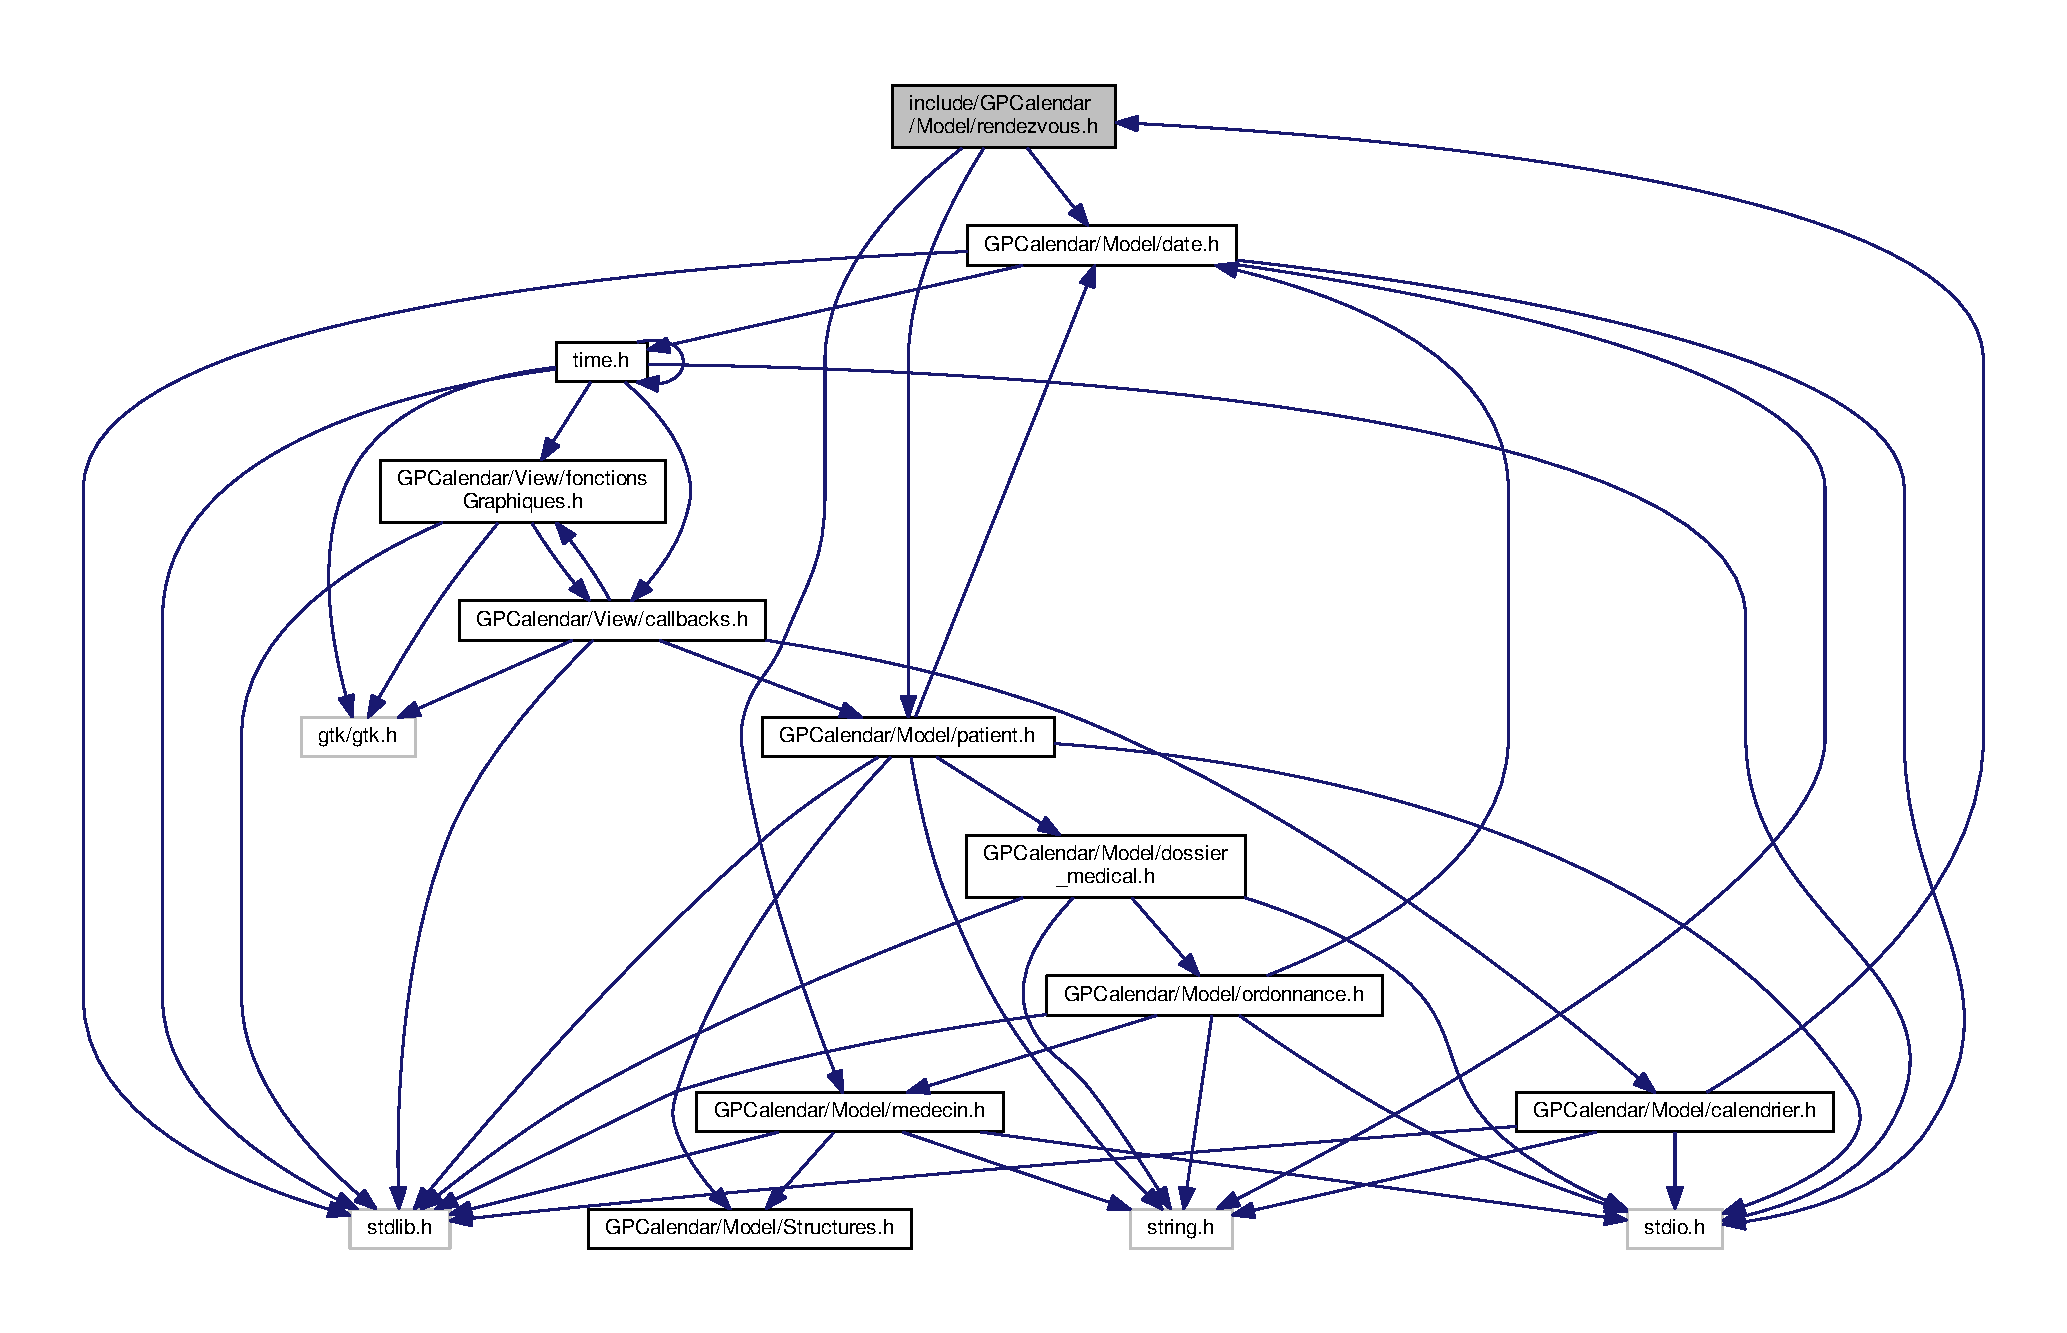
\includegraphics[width=350pt]{rendezvous_8h__incl}
\end{center}
\end{figure}
Ce graphe montre quels fichiers incluent directement ou indirectement ce fichier \-:
\nopagebreak
\begin{figure}[H]
\begin{center}
\leavevmode
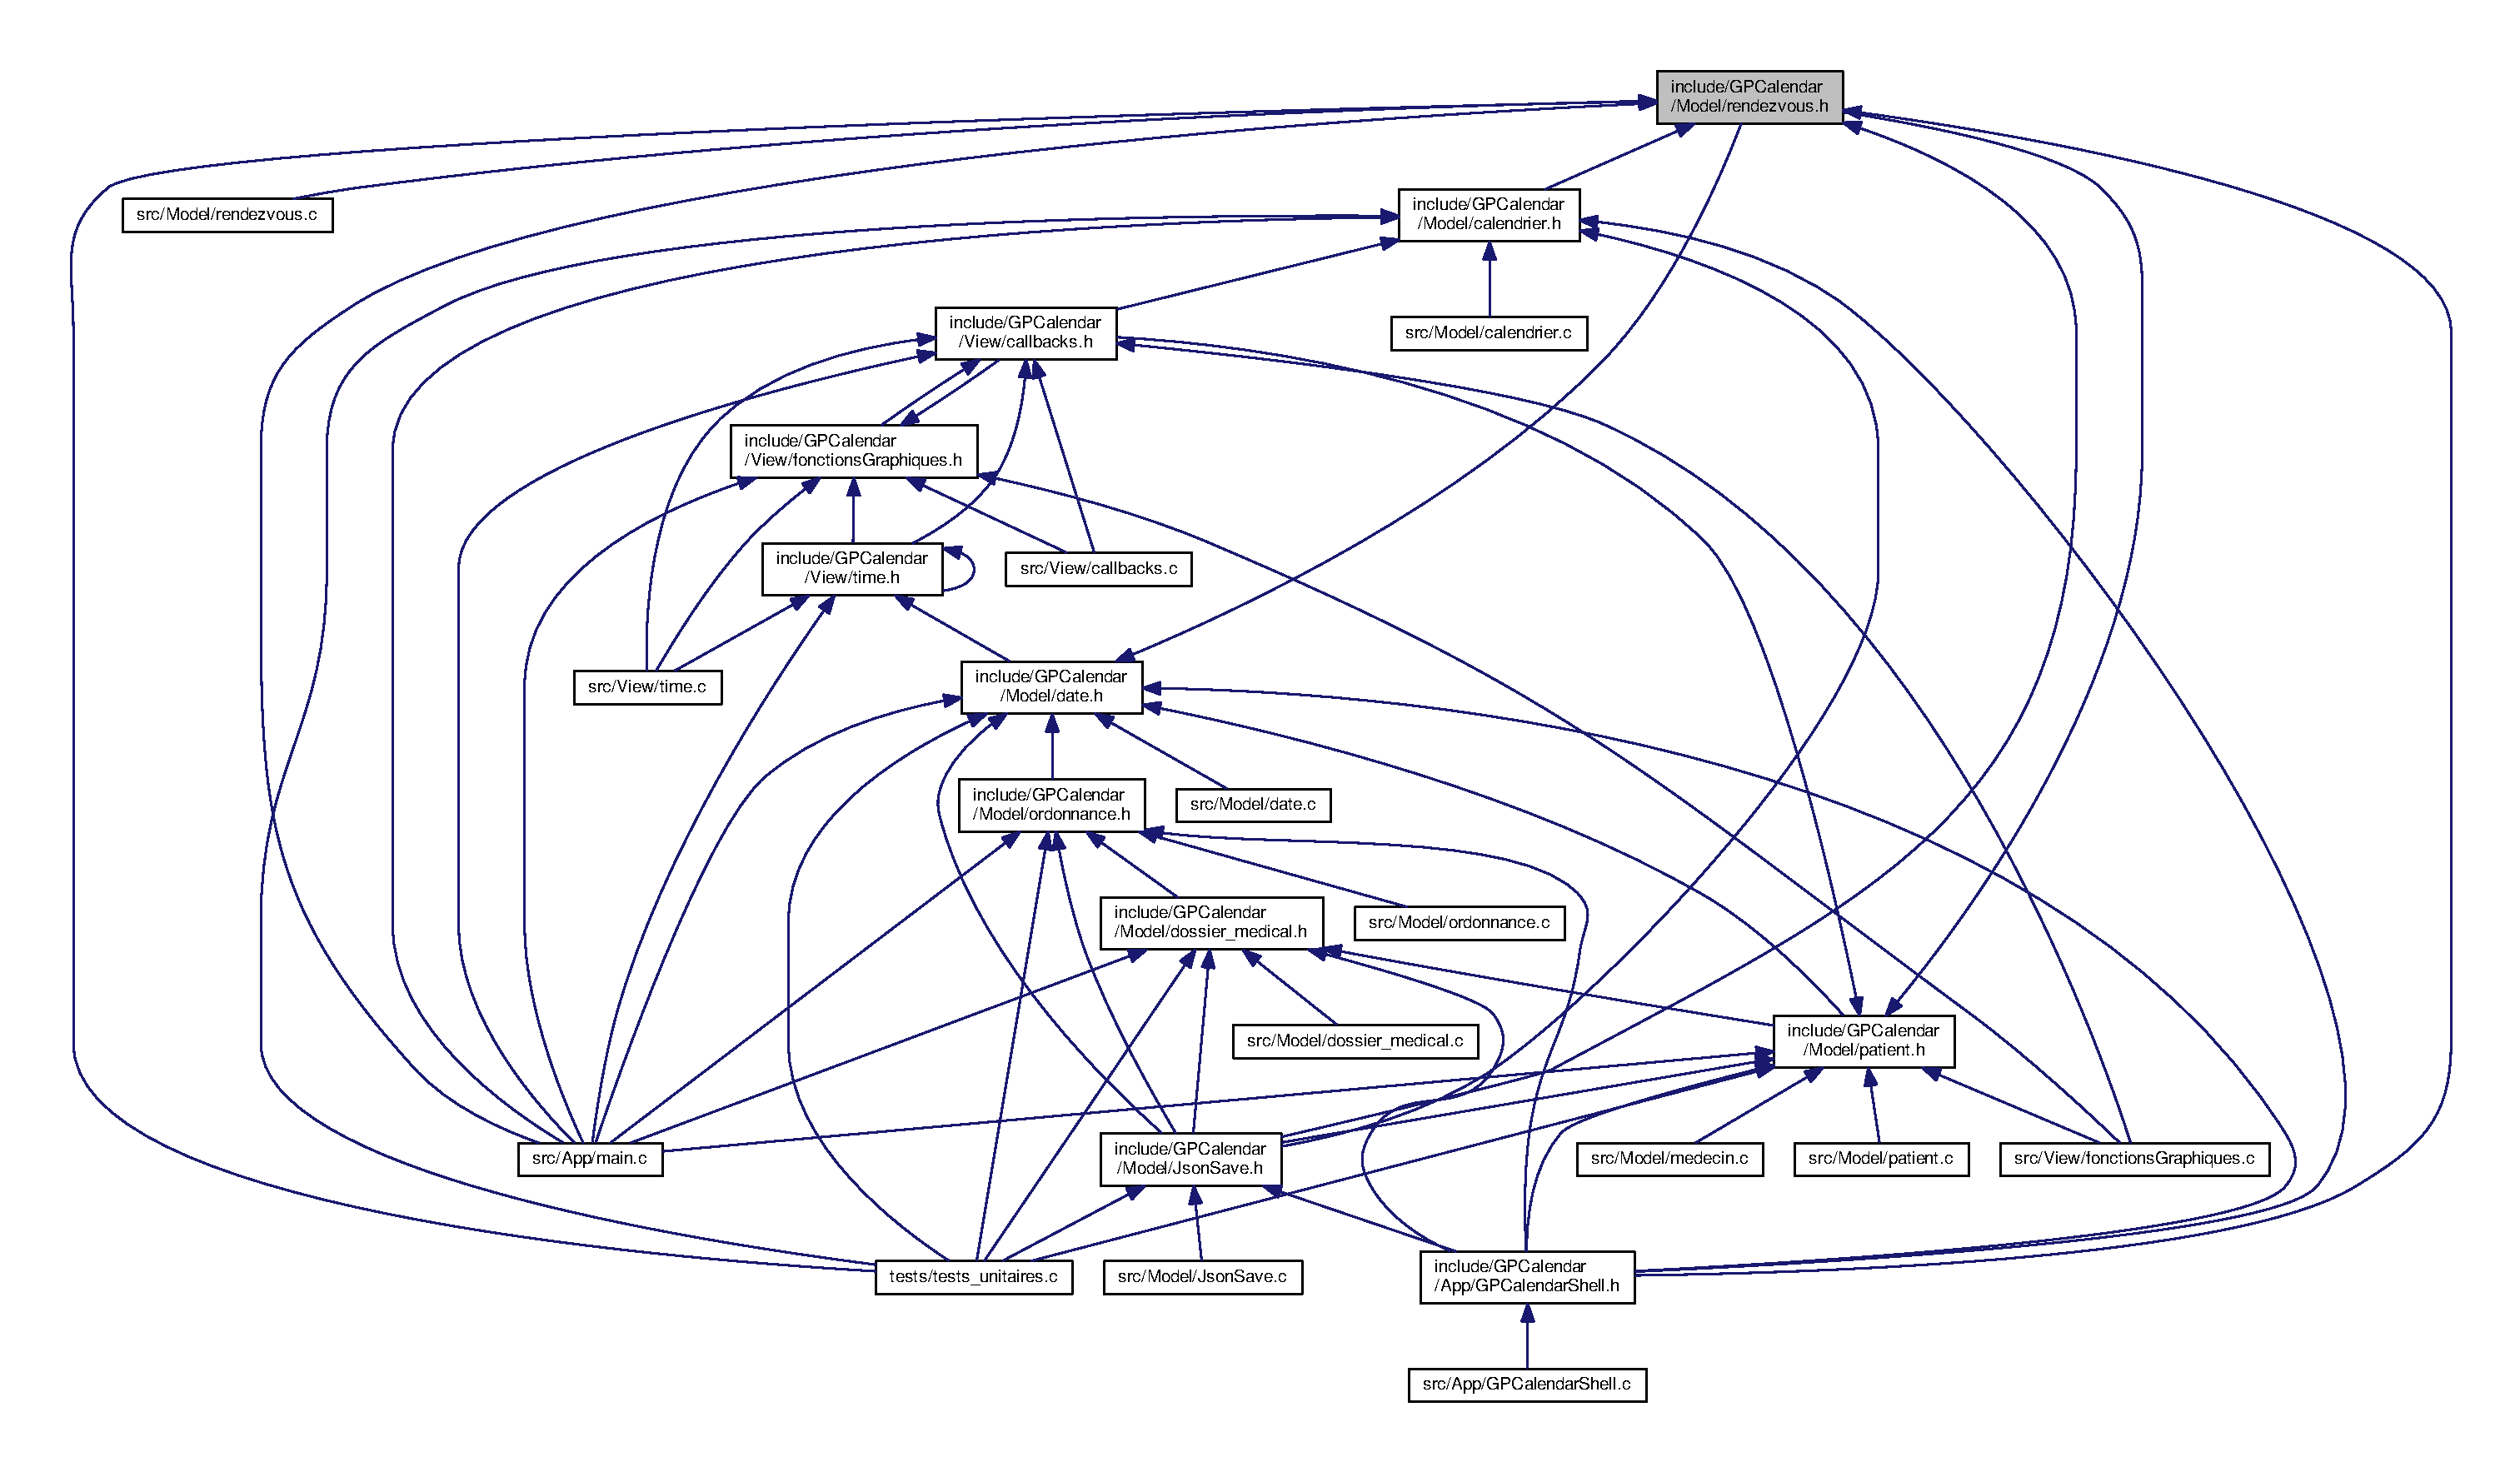
\includegraphics[width=350pt]{rendezvous_8h__dep__incl}
\end{center}
\end{figure}
\subsection*{Structures de données}
\begin{DoxyCompactItemize}
\item 
struct \hyperlink{struct_rendez_vous}{Rendez\-Vous}
\end{DoxyCompactItemize}
\subsection*{Fonctions}
\begin{DoxyCompactItemize}
\item 
\hyperlink{struct_rendez_vous}{Rendez\-Vous} $\ast$ \hyperlink{rendezvous_8h_ae62501b5f409d83dc182560bbb97a276}{Creer\-Rendez\-Vous} (int an, int mois, int jour, double heure\-\_\-debut, int duree, char $\ast$lieu, \hyperlink{struct_patient}{Patient} $\ast$patient, \hyperlink{struct_medecin}{Medecin} $\ast$medecin, char $\ast$motif)
\item 
void \hyperlink{rendezvous_8h_a1d5659faf0a3498ce343e7d14015489d}{Free\-Rendez\-Vous} (\hyperlink{struct_rendez_vous}{Rendez\-Vous} $\ast$rdv)
\item 
int \hyperlink{rendezvous_8h_a78731530177f360d1452c1dbe7c8bdef}{Annuler\-Rendez\-Vous} (\hyperlink{struct_rendez_vous}{Rendez\-Vous} $\ast$rdv)
\item 
\hyperlink{struct_rendez_vous}{Rendez\-Vous} $\ast$ \hyperlink{rendezvous_8h_a75dec28fc6cc82183dec57c710e87b0e}{Deplacer\-Rendez\-Vous} (\hyperlink{struct_rendez_vous}{Rendez\-Vous} $\ast$rdv, int n\-\_\-an, int n\-\_\-mois, int n\-\_\-jour, double n\-\_\-heure\-\_\-debut, int n\-\_\-duree)
\end{DoxyCompactItemize}


\subsection{Documentation des fonctions}
\hypertarget{rendezvous_8h_a78731530177f360d1452c1dbe7c8bdef}{\index{rendezvous.\-h@{rendezvous.\-h}!Annuler\-Rendez\-Vous@{Annuler\-Rendez\-Vous}}
\index{Annuler\-Rendez\-Vous@{Annuler\-Rendez\-Vous}!rendezvous.h@{rendezvous.\-h}}
\subsubsection[{Annuler\-Rendez\-Vous}]{\setlength{\rightskip}{0pt plus 5cm}int Annuler\-Rendez\-Vous (
\begin{DoxyParamCaption}
\item[{{\bf Rendez\-Vous} $\ast$}]{rdv}
\end{DoxyParamCaption}
)}}\label{rendezvous_8h_a78731530177f360d1452c1dbe7c8bdef}
Annuler\-Rendez\-Vous \-: Annuler un \hyperlink{struct_rendez_vous}{Rendez\-Vous}, l'initialiser à vide 
\begin{DoxyParams}{Paramètres}
{\em rdv} & \-: le rdv qu'on veut annuler \\
\hline
\end{DoxyParams}
\begin{DoxyReturn}{Renvoie}
1 si le rdv a bien été annulé 
\end{DoxyReturn}
\hypertarget{rendezvous_8h_ae62501b5f409d83dc182560bbb97a276}{\index{rendezvous.\-h@{rendezvous.\-h}!Creer\-Rendez\-Vous@{Creer\-Rendez\-Vous}}
\index{Creer\-Rendez\-Vous@{Creer\-Rendez\-Vous}!rendezvous.h@{rendezvous.\-h}}
\subsubsection[{Creer\-Rendez\-Vous}]{\setlength{\rightskip}{0pt plus 5cm}{\bf Rendez\-Vous}$\ast$ Creer\-Rendez\-Vous (
\begin{DoxyParamCaption}
\item[{int}]{an, }
\item[{int}]{mois, }
\item[{int}]{jour, }
\item[{double}]{heure\-\_\-debut, }
\item[{int}]{duree, }
\item[{char $\ast$}]{lieu, }
\item[{{\bf Patient} $\ast$}]{patient, }
\item[{{\bf Medecin} $\ast$}]{medecin, }
\item[{char $\ast$}]{motif}
\end{DoxyParamCaption}
)}}\label{rendezvous_8h_ae62501b5f409d83dc182560bbb97a276}
Creer\-Rendez\-Vous \-: Creer dynamiquement un objet \hyperlink{struct_rendez_vous}{Rendez\-Vous} 
\begin{DoxyParams}{Paramètres}
{\em an} & \-: l'annee \\
\hline
{\em mois} & \-: le mois \\
\hline
{\em jour} & \-: le jour \\
\hline
{\em heure\-\_\-debut} & \-: l'heure ((sous forme de double \-: 16.\-5 $<$=$>$ 16\-H30) du début du rdv \\
\hline
{\em duree} & \-: la duree du rdv, avec on détermine heure\-\_\-fin du rdv \\
\hline
{\em lieu} & \-: le lieu du rdv \\
\hline
{\em patient} & \-: le patient demandant le rdv \\
\hline
{\em médecin} & \-: le medecin choisi pour le rdv \\
\hline
{\em motif} & \-: le motif du rdv \\
\hline
\end{DoxyParams}
\begin{DoxyReturn}{Renvoie}
le rdv créé 
\end{DoxyReturn}
\hypertarget{rendezvous_8h_a75dec28fc6cc82183dec57c710e87b0e}{\index{rendezvous.\-h@{rendezvous.\-h}!Deplacer\-Rendez\-Vous@{Deplacer\-Rendez\-Vous}}
\index{Deplacer\-Rendez\-Vous@{Deplacer\-Rendez\-Vous}!rendezvous.h@{rendezvous.\-h}}
\subsubsection[{Deplacer\-Rendez\-Vous}]{\setlength{\rightskip}{0pt plus 5cm}{\bf Rendez\-Vous}$\ast$ Deplacer\-Rendez\-Vous (
\begin{DoxyParamCaption}
\item[{{\bf Rendez\-Vous} $\ast$}]{rdv, }
\item[{int}]{n\-\_\-an, }
\item[{int}]{n\-\_\-mois, }
\item[{int}]{n\-\_\-jour, }
\item[{double}]{n\-\_\-heure\-\_\-debut, }
\item[{int}]{n\-\_\-duree}
\end{DoxyParamCaption}
)}}\label{rendezvous_8h_a75dec28fc6cc82183dec57c710e87b0e}
Deplacer\-Rendez\-Vous \-: Deplacer un \hyperlink{struct_rendez_vous}{Rendez\-Vous} 
\begin{DoxyParams}{Paramètres}
{\em rdv} & \-: le rdv qu'on veut deplacer \\
\hline
{\em n\-\_\-an} & \-: nouvelle année du rdv \\
\hline
{\em n\-\_\-mois} & \-: nouveau mois du rdv \\
\hline
{\em n\-\_\-jour} & \-: nouveau jour du rdv \\
\hline
{\em n\-\_\-heure} & \-: nouvelle heure du rdv \\
\hline
{\em n\-\_\-minute} & \-: nouvelle minute de l'horaire du rdv \\
\hline
{\em n\-\_\-duree} & \-: nouvelle duree du rdv \\
\hline
\end{DoxyParams}
\begin{DoxyReturn}{Renvoie}
le rdv deplacé 
\end{DoxyReturn}
\hypertarget{rendezvous_8h_a1d5659faf0a3498ce343e7d14015489d}{\index{rendezvous.\-h@{rendezvous.\-h}!Free\-Rendez\-Vous@{Free\-Rendez\-Vous}}
\index{Free\-Rendez\-Vous@{Free\-Rendez\-Vous}!rendezvous.h@{rendezvous.\-h}}
\subsubsection[{Free\-Rendez\-Vous}]{\setlength{\rightskip}{0pt plus 5cm}void Free\-Rendez\-Vous (
\begin{DoxyParamCaption}
\item[{{\bf Rendez\-Vous} $\ast$}]{rdv}
\end{DoxyParamCaption}
)}}\label{rendezvous_8h_a1d5659faf0a3498ce343e7d14015489d}
Free\-Rendez\-Vous \-: Free un objet rdv (seulement sa date et le rdv en lui-\/même), on ne touche pas au patient et au medecin car ils existent toujours dans d'autres rdv 
\begin{DoxyParams}{Paramètres}
{\em rdv} & \-: le rdv à free \\
\hline
\end{DoxyParams}

\hypertarget{_structures_8h}{\section{Référence du fichier include/\-G\-P\-Calendar/\-Model/\-Structures.h}
\label{_structures_8h}\index{include/\-G\-P\-Calendar/\-Model/\-Structures.\-h@{include/\-G\-P\-Calendar/\-Model/\-Structures.\-h}}
}
Ce graphe montre quels fichiers incluent directement ou indirectement ce fichier \-:
\nopagebreak
\begin{figure}[H]
\begin{center}
\leavevmode
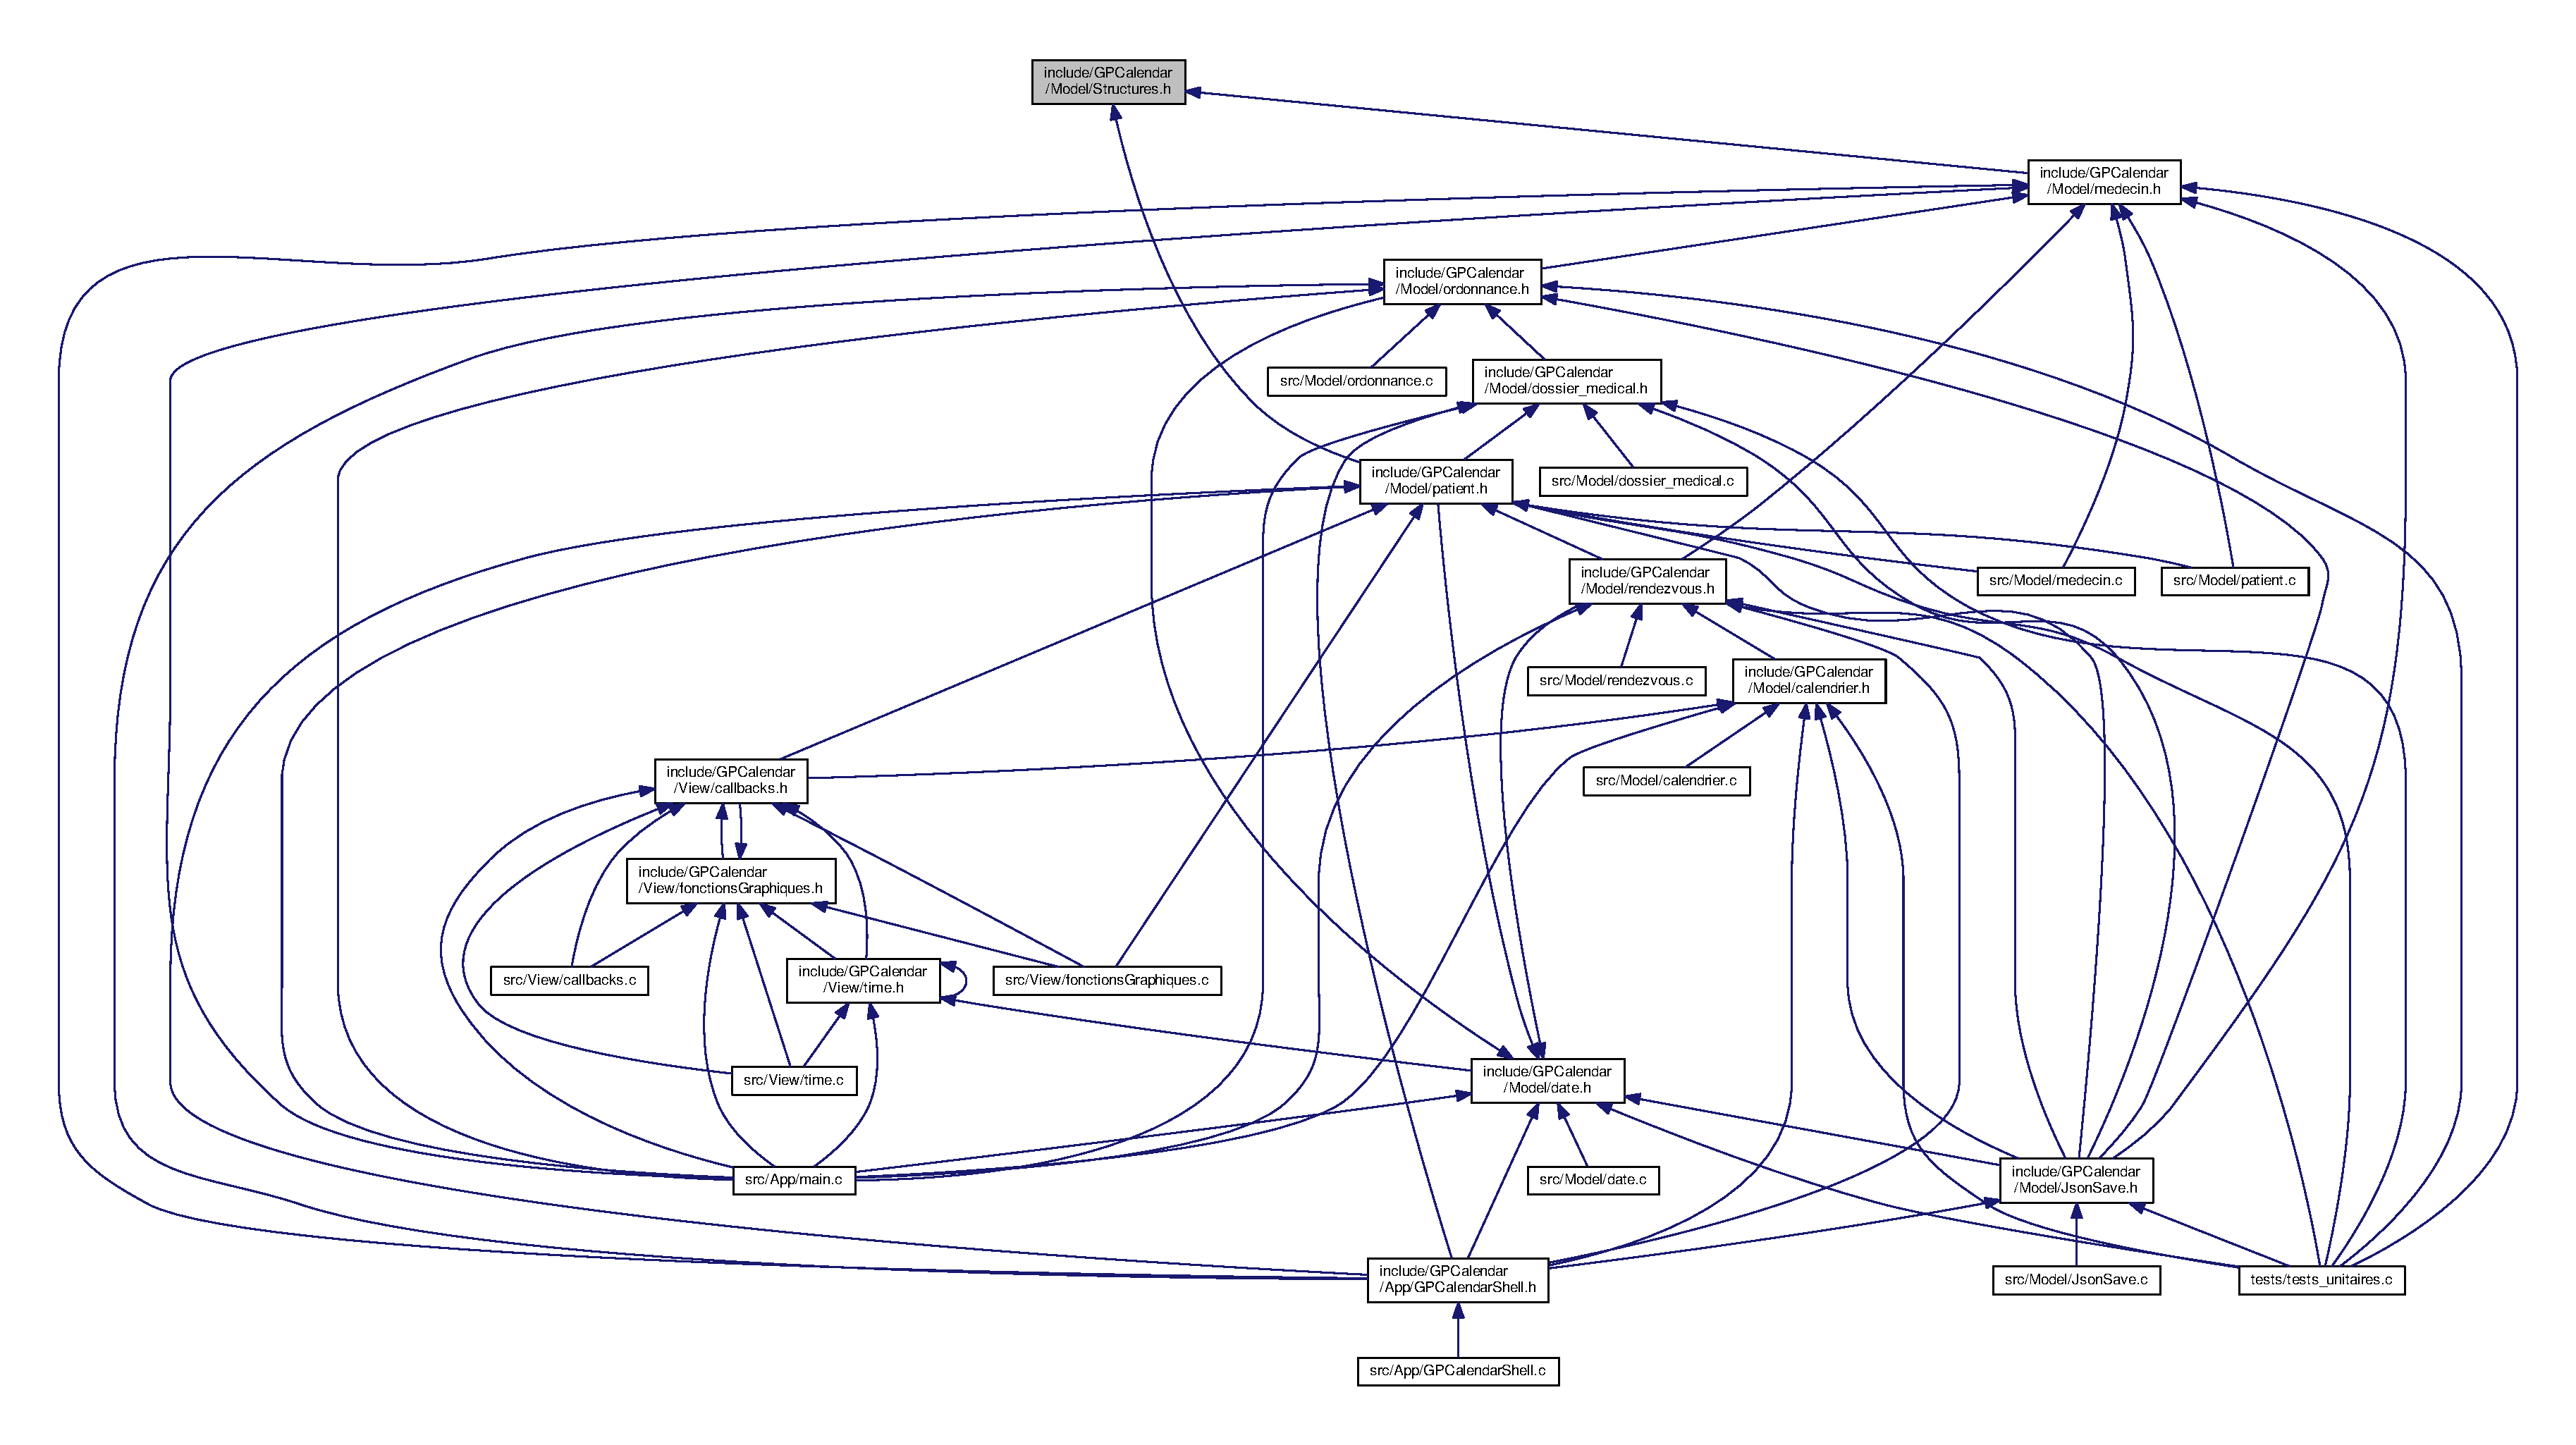
\includegraphics[width=350pt]{_structures_8h__dep__incl}
\end{center}
\end{figure}
\subsection*{Définitions de type}
\begin{DoxyCompactItemize}
\item 
typedef struct \hyperlink{struct_patient}{Patient} \hyperlink{_structures_8h_af55d4995d5670395a27c07bd4a180eae}{Patient}
\item 
typedef struct \hyperlink{struct_list_patient}{List\-Patient} \hyperlink{_structures_8h_ac11c306f3f635ec6ca423604d4168956}{List\-Patient}
\item 
typedef struct \hyperlink{struct_medecin}{Medecin} \hyperlink{_structures_8h_a1d11513fc6a5221e68363bffce50b69c}{Medecin}
\item 
typedef struct \hyperlink{struct_list_medecin}{List\-Medecin} \hyperlink{_structures_8h_a1cd3959199861129f521ded9543df622}{List\-Medecin}
\end{DoxyCompactItemize}


\subsection{Documentation des définitions de type}
\hypertarget{_structures_8h_a1cd3959199861129f521ded9543df622}{\index{Structures.\-h@{Structures.\-h}!List\-Medecin@{List\-Medecin}}
\index{List\-Medecin@{List\-Medecin}!Structures.h@{Structures.\-h}}
\subsubsection[{List\-Medecin}]{\setlength{\rightskip}{0pt plus 5cm}typedef struct {\bf List\-Medecin} {\bf List\-Medecin}}}\label{_structures_8h_a1cd3959199861129f521ded9543df622}
\hypertarget{_structures_8h_ac11c306f3f635ec6ca423604d4168956}{\index{Structures.\-h@{Structures.\-h}!List\-Patient@{List\-Patient}}
\index{List\-Patient@{List\-Patient}!Structures.h@{Structures.\-h}}
\subsubsection[{List\-Patient}]{\setlength{\rightskip}{0pt plus 5cm}typedef struct {\bf List\-Patient} {\bf List\-Patient}}}\label{_structures_8h_ac11c306f3f635ec6ca423604d4168956}
\hypertarget{_structures_8h_a1d11513fc6a5221e68363bffce50b69c}{\index{Structures.\-h@{Structures.\-h}!Medecin@{Medecin}}
\index{Medecin@{Medecin}!Structures.h@{Structures.\-h}}
\subsubsection[{Medecin}]{\setlength{\rightskip}{0pt plus 5cm}typedef struct {\bf Medecin} {\bf Medecin}}}\label{_structures_8h_a1d11513fc6a5221e68363bffce50b69c}
\hypertarget{_structures_8h_af55d4995d5670395a27c07bd4a180eae}{\index{Structures.\-h@{Structures.\-h}!Patient@{Patient}}
\index{Patient@{Patient}!Structures.h@{Structures.\-h}}
\subsubsection[{Patient}]{\setlength{\rightskip}{0pt plus 5cm}typedef struct {\bf Patient} {\bf Patient}}}\label{_structures_8h_af55d4995d5670395a27c07bd4a180eae}

\hypertarget{callbacks_8h}{\section{Référence du fichier include/\-G\-P\-Calendar/\-View/callbacks.h}
\label{callbacks_8h}\index{include/\-G\-P\-Calendar/\-View/callbacks.\-h@{include/\-G\-P\-Calendar/\-View/callbacks.\-h}}
}


Provides basic unit testing functions declaration.  


{\ttfamily \#include \char`\"{}G\-P\-Calendar/\-View/fonctions\-Graphiques.\-h\char`\"{}}\\*
{\ttfamily \#include \char`\"{}G\-P\-Calendar/\-Model/patient.\-h\char`\"{}}\\*
{\ttfamily \#include \char`\"{}G\-P\-Calendar/\-Model/calendrier.\-h\char`\"{}}\\*
{\ttfamily \#include $<$gtk/gtk.\-h$>$}\\*
{\ttfamily \#include $<$stdlib.\-h$>$}\\*
Graphe des dépendances par inclusion de callbacks.\-h\-:
\nopagebreak
\begin{figure}[H]
\begin{center}
\leavevmode
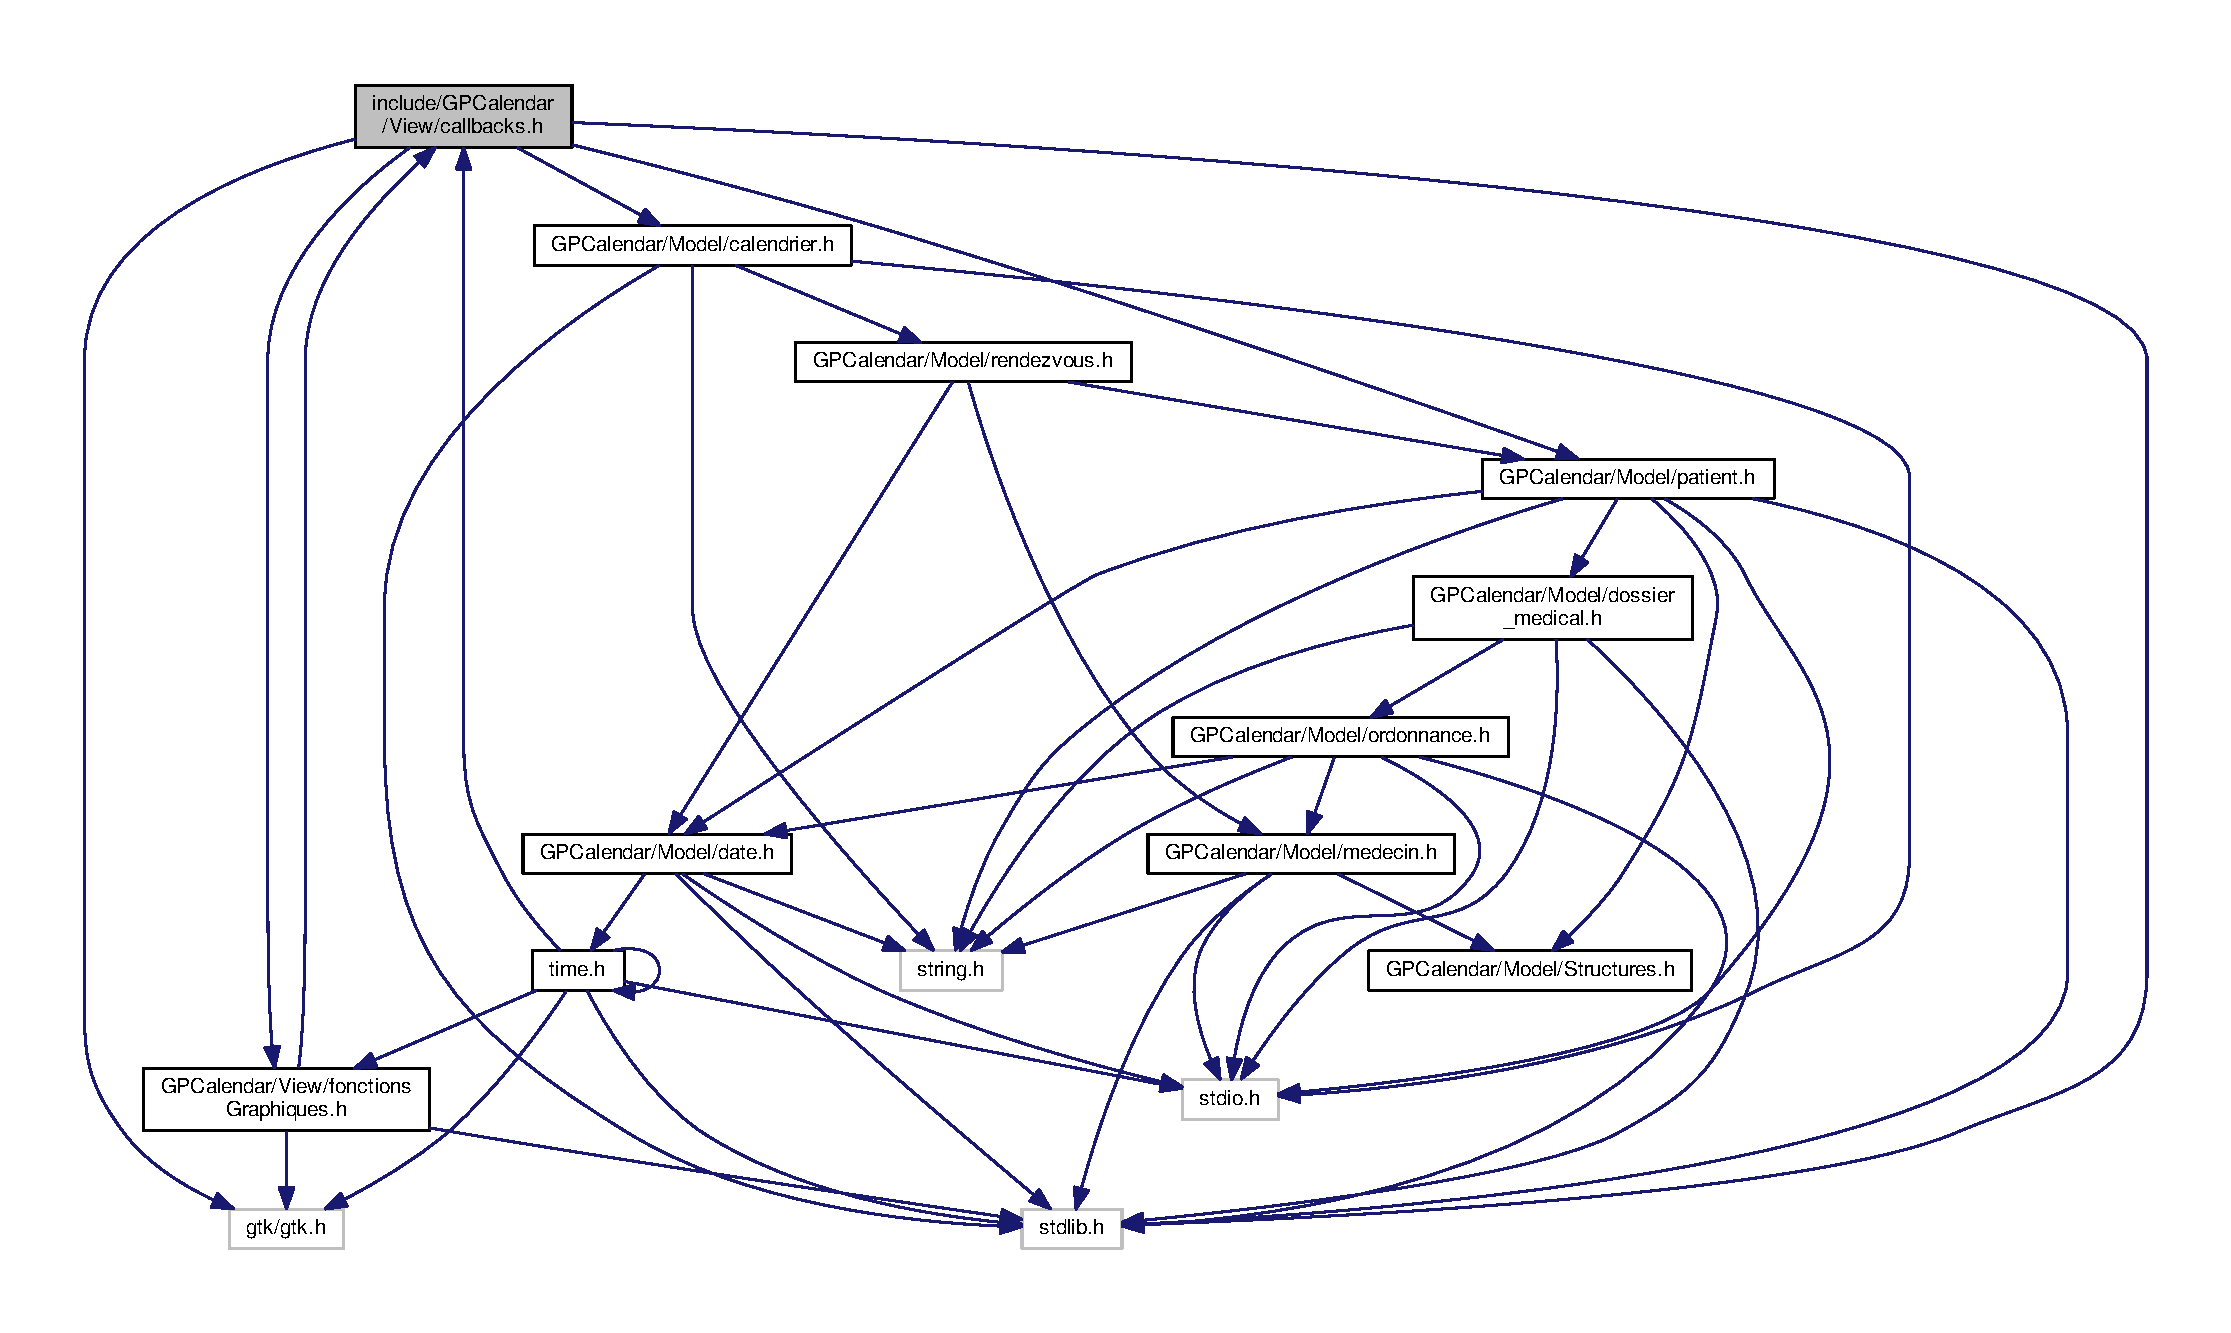
\includegraphics[width=350pt]{callbacks_8h__incl}
\end{center}
\end{figure}
Ce graphe montre quels fichiers incluent directement ou indirectement ce fichier \-:
\nopagebreak
\begin{figure}[H]
\begin{center}
\leavevmode
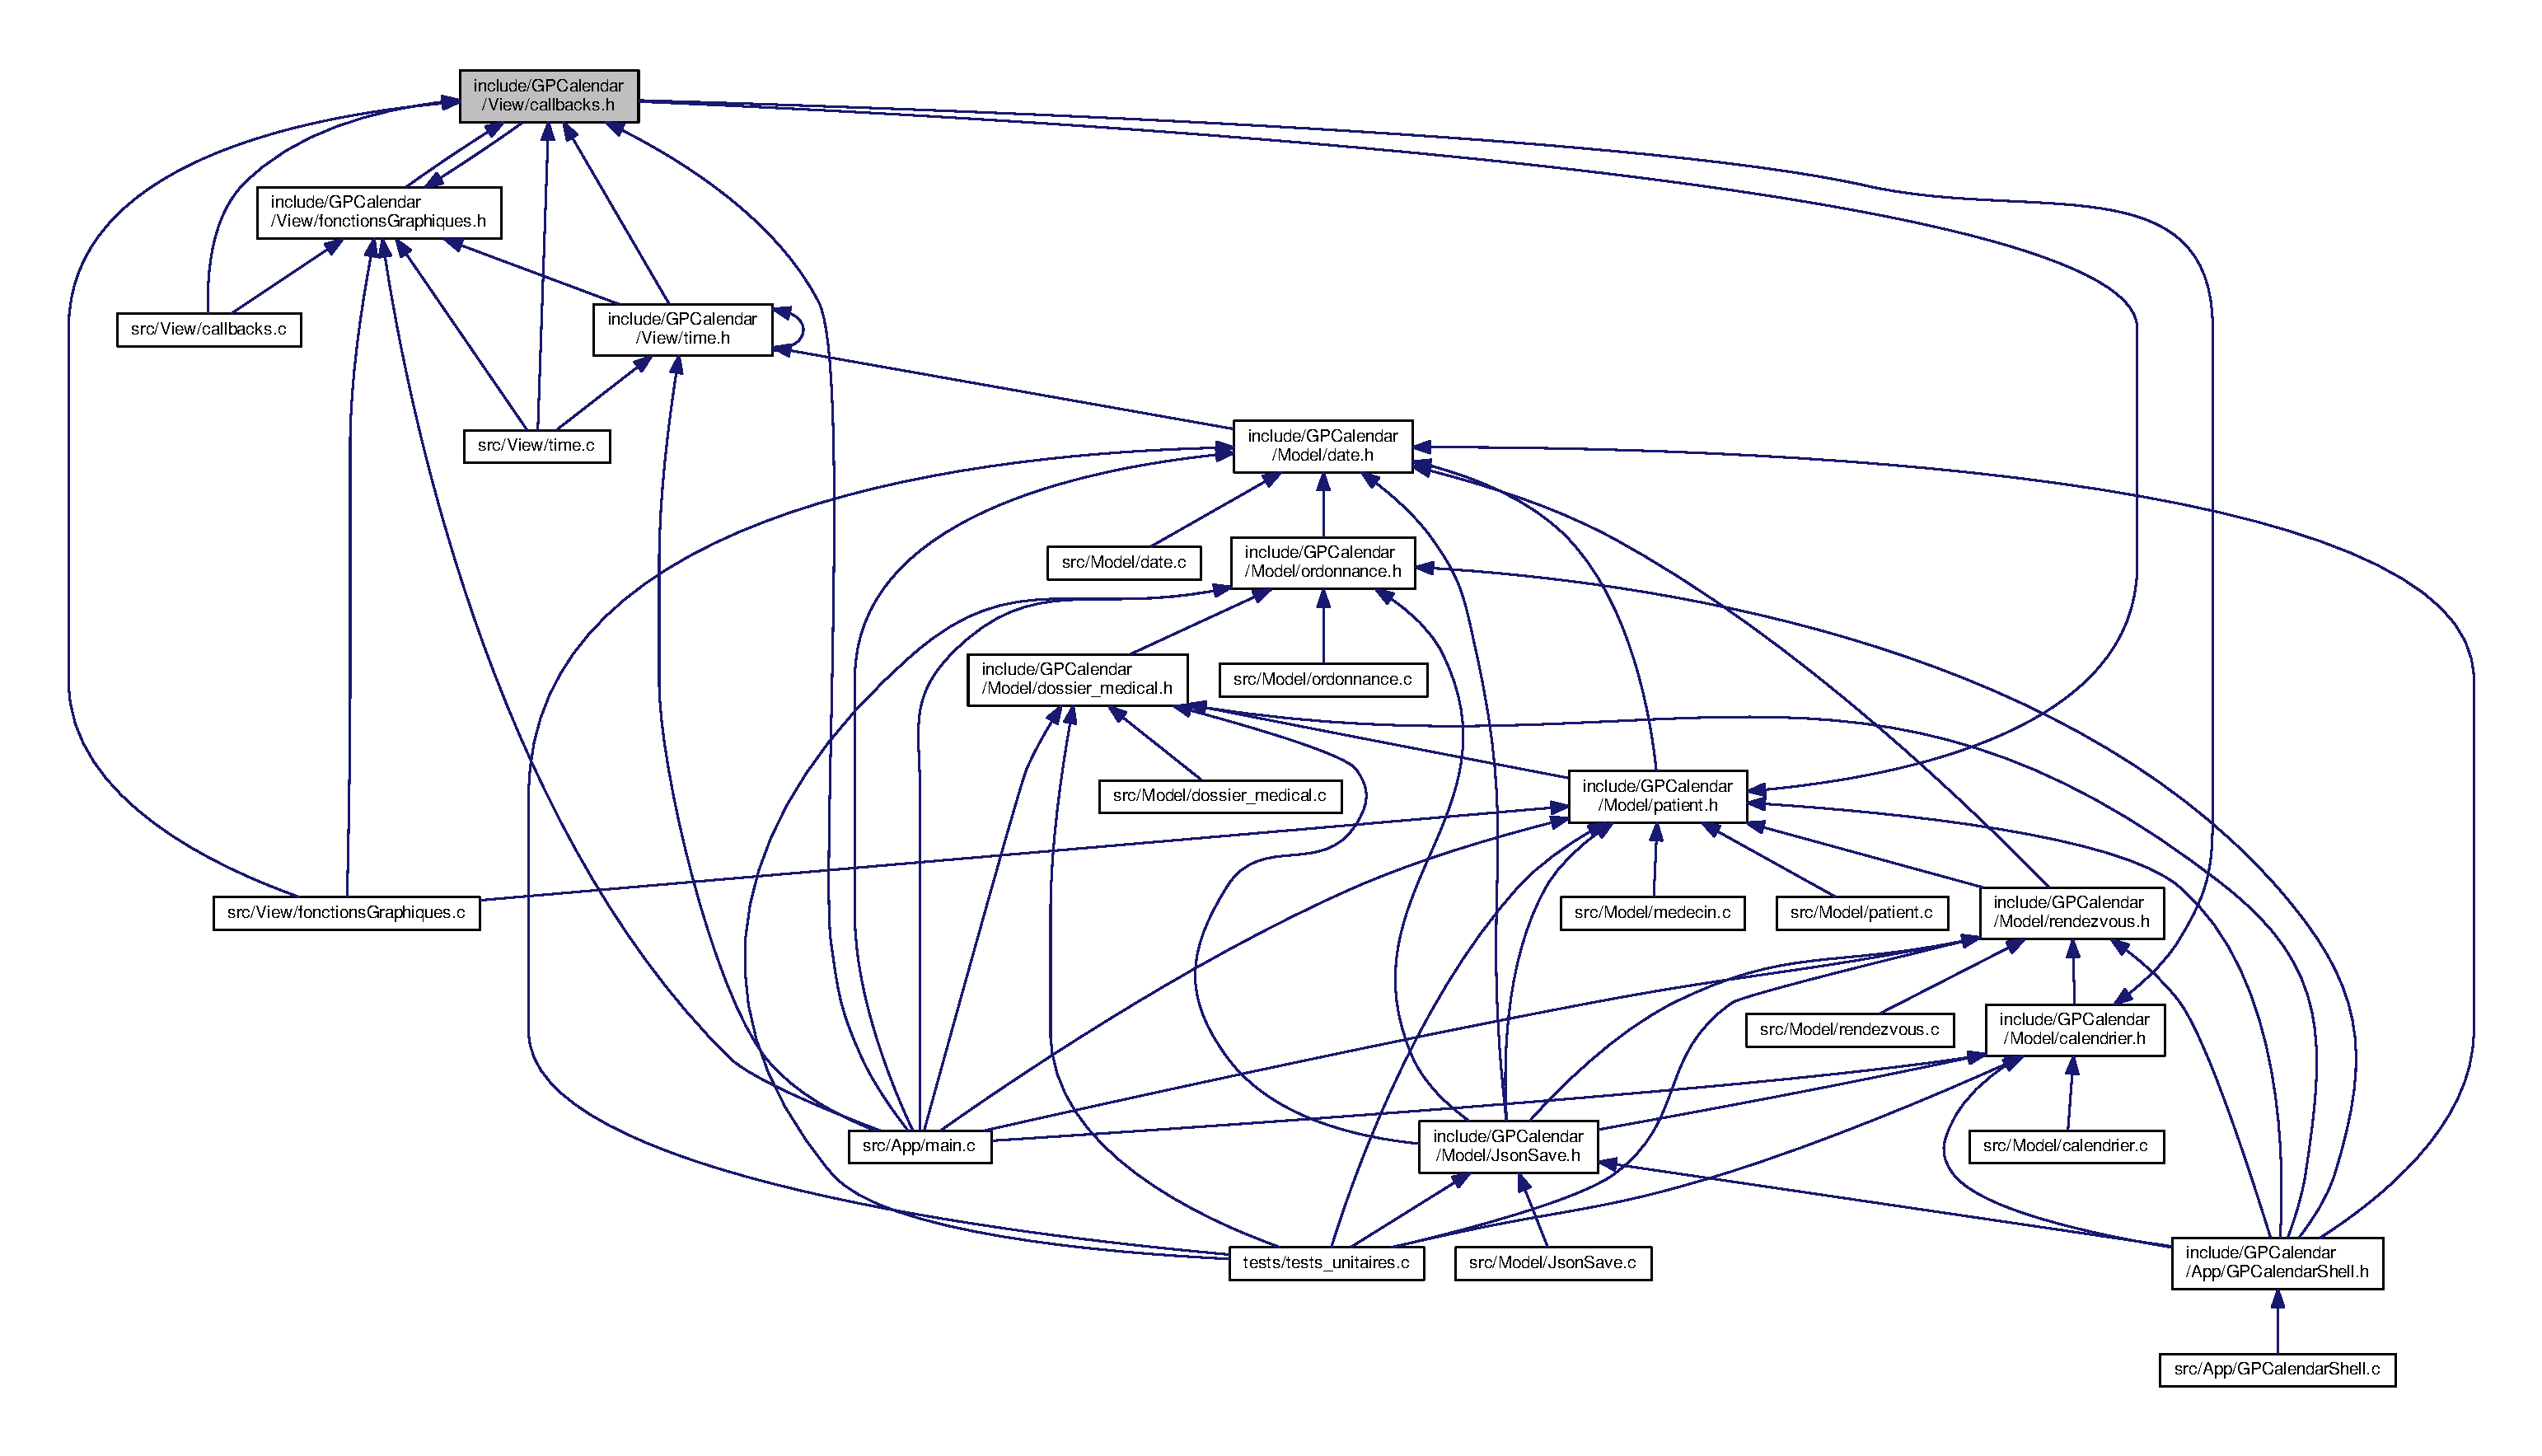
\includegraphics[width=350pt]{callbacks_8h__dep__incl}
\end{center}
\end{figure}
\subsection*{Structures de données}
\begin{DoxyCompactItemize}
\item 
struct \hyperlink{struct_data}{Data}
\item 
struct \hyperlink{struct_data_r_d_v}{Data\-R\-D\-V}
\end{DoxyCompactItemize}
\subsection*{Définitions de type}
\begin{DoxyCompactItemize}
\item 
typedef struct \hyperlink{struct_data}{Data} \hyperlink{callbacks_8h_aa29088b0ebf449924c098ffbc3fb8350}{data\-Patient}
\item 
typedef struct \hyperlink{struct_data_r_d_v}{Data\-R\-D\-V} \hyperlink{callbacks_8h_aabd3ef47a662e3ae616f0f2025264e05}{data\-Rdv}
\end{DoxyCompactItemize}
\subsection*{Fonctions}
\begin{DoxyCompactItemize}
\item 
void \hyperlink{callbacks_8h_a1c6426a0d3e99e004d82d19d6217c285}{cb\-\_\-create\-\_\-entry} (Gtk\-Widget $\ast$p\-\_\-widget, gpointer user\-\_\-data)
\item 
void \hyperlink{callbacks_8h_a2d84262978bfceef5a73b41fcf73ab79}{cb\-\_\-create\-\_\-entry1} (Gtk\-Widget $\ast$p\-\_\-widget, gpointer user\-\_\-data)
\item 
void \hyperlink{callbacks_8h_aaa57391a0ab9a2a118578182fe80dd44}{cb\-\_\-clic\-Sur\-Plus} (Gtk\-Widget $\ast$widget, gpointer data)
\item 
void \hyperlink{callbacks_8h_a4f53175f04259ff4ad1e805fc6aabe41}{cb\-\_\-recherche\-Patient} (Gtk\-Widget $\ast$widget, gpointer data)
\item 
void \hyperlink{callbacks_8h_a12248d7cb83a202f6b18f1cc8de967e4}{cb\-\_\-creation\-Patient} (Gtk\-Widget $\ast$widget, gpointer data)
\item 
void \hyperlink{callbacks_8h_a695fea329709691f3aabb1a8413628d8}{cb\-\_\-creation\-R\-D\-V} (Gtk\-Widget $\ast$widget, gpointer data)
\item 
void \hyperlink{callbacks_8h_a38edcb4bfb81adbb28c91e175520acee}{enter\-\_\-callback} (Gtk\-Widget $\ast$widget, Gtk\-Widget $\ast$entry)
\end{DoxyCompactItemize}


\subsection{Description détaillée}
Provides basic unit testing functions declaration. 

\subsection{Documentation des définitions de type}
\hypertarget{callbacks_8h_aa29088b0ebf449924c098ffbc3fb8350}{\index{callbacks.\-h@{callbacks.\-h}!data\-Patient@{data\-Patient}}
\index{data\-Patient@{data\-Patient}!callbacks.h@{callbacks.\-h}}
\subsubsection[{data\-Patient}]{\setlength{\rightskip}{0pt plus 5cm}typedef struct {\bf Data} {\bf data\-Patient}}}\label{callbacks_8h_aa29088b0ebf449924c098ffbc3fb8350}
\hypertarget{callbacks_8h_aabd3ef47a662e3ae616f0f2025264e05}{\index{callbacks.\-h@{callbacks.\-h}!data\-Rdv@{data\-Rdv}}
\index{data\-Rdv@{data\-Rdv}!callbacks.h@{callbacks.\-h}}
\subsubsection[{data\-Rdv}]{\setlength{\rightskip}{0pt plus 5cm}typedef struct {\bf Data\-R\-D\-V} {\bf data\-Rdv}}}\label{callbacks_8h_aabd3ef47a662e3ae616f0f2025264e05}


\subsection{Documentation des fonctions}
\hypertarget{callbacks_8h_aaa57391a0ab9a2a118578182fe80dd44}{\index{callbacks.\-h@{callbacks.\-h}!cb\-\_\-clic\-Sur\-Plus@{cb\-\_\-clic\-Sur\-Plus}}
\index{cb\-\_\-clic\-Sur\-Plus@{cb\-\_\-clic\-Sur\-Plus}!callbacks.h@{callbacks.\-h}}
\subsubsection[{cb\-\_\-clic\-Sur\-Plus}]{\setlength{\rightskip}{0pt plus 5cm}void cb\-\_\-clic\-Sur\-Plus (
\begin{DoxyParamCaption}
\item[{Gtk\-Widget $\ast$}]{widget, }
\item[{gpointer}]{data}
\end{DoxyParamCaption}
)}}\label{callbacks_8h_aaa57391a0ab9a2a118578182fe80dd44}
\hypertarget{callbacks_8h_a1c6426a0d3e99e004d82d19d6217c285}{\index{callbacks.\-h@{callbacks.\-h}!cb\-\_\-create\-\_\-entry@{cb\-\_\-create\-\_\-entry}}
\index{cb\-\_\-create\-\_\-entry@{cb\-\_\-create\-\_\-entry}!callbacks.h@{callbacks.\-h}}
\subsubsection[{cb\-\_\-create\-\_\-entry}]{\setlength{\rightskip}{0pt plus 5cm}void cb\-\_\-create\-\_\-entry (
\begin{DoxyParamCaption}
\item[{Gtk\-Widget $\ast$}]{p\-\_\-widget, }
\item[{gpointer}]{user\-\_\-data}
\end{DoxyParamCaption}
)}}\label{callbacks_8h_a1c6426a0d3e99e004d82d19d6217c285}
\hypertarget{callbacks_8h_a2d84262978bfceef5a73b41fcf73ab79}{\index{callbacks.\-h@{callbacks.\-h}!cb\-\_\-create\-\_\-entry1@{cb\-\_\-create\-\_\-entry1}}
\index{cb\-\_\-create\-\_\-entry1@{cb\-\_\-create\-\_\-entry1}!callbacks.h@{callbacks.\-h}}
\subsubsection[{cb\-\_\-create\-\_\-entry1}]{\setlength{\rightskip}{0pt plus 5cm}void cb\-\_\-create\-\_\-entry1 (
\begin{DoxyParamCaption}
\item[{Gtk\-Widget $\ast$}]{p\-\_\-widget, }
\item[{gpointer}]{user\-\_\-data}
\end{DoxyParamCaption}
)}}\label{callbacks_8h_a2d84262978bfceef5a73b41fcf73ab79}
\hypertarget{callbacks_8h_a12248d7cb83a202f6b18f1cc8de967e4}{\index{callbacks.\-h@{callbacks.\-h}!cb\-\_\-creation\-Patient@{cb\-\_\-creation\-Patient}}
\index{cb\-\_\-creation\-Patient@{cb\-\_\-creation\-Patient}!callbacks.h@{callbacks.\-h}}
\subsubsection[{cb\-\_\-creation\-Patient}]{\setlength{\rightskip}{0pt plus 5cm}void cb\-\_\-creation\-Patient (
\begin{DoxyParamCaption}
\item[{Gtk\-Widget $\ast$}]{widget, }
\item[{gpointer}]{data}
\end{DoxyParamCaption}
)}}\label{callbacks_8h_a12248d7cb83a202f6b18f1cc8de967e4}
\hypertarget{callbacks_8h_a695fea329709691f3aabb1a8413628d8}{\index{callbacks.\-h@{callbacks.\-h}!cb\-\_\-creation\-R\-D\-V@{cb\-\_\-creation\-R\-D\-V}}
\index{cb\-\_\-creation\-R\-D\-V@{cb\-\_\-creation\-R\-D\-V}!callbacks.h@{callbacks.\-h}}
\subsubsection[{cb\-\_\-creation\-R\-D\-V}]{\setlength{\rightskip}{0pt plus 5cm}void cb\-\_\-creation\-R\-D\-V (
\begin{DoxyParamCaption}
\item[{Gtk\-Widget $\ast$}]{widget, }
\item[{gpointer}]{data}
\end{DoxyParamCaption}
)}}\label{callbacks_8h_a695fea329709691f3aabb1a8413628d8}
\hypertarget{callbacks_8h_a4f53175f04259ff4ad1e805fc6aabe41}{\index{callbacks.\-h@{callbacks.\-h}!cb\-\_\-recherche\-Patient@{cb\-\_\-recherche\-Patient}}
\index{cb\-\_\-recherche\-Patient@{cb\-\_\-recherche\-Patient}!callbacks.h@{callbacks.\-h}}
\subsubsection[{cb\-\_\-recherche\-Patient}]{\setlength{\rightskip}{0pt plus 5cm}void cb\-\_\-recherche\-Patient (
\begin{DoxyParamCaption}
\item[{Gtk\-Widget $\ast$}]{widget, }
\item[{gpointer}]{data}
\end{DoxyParamCaption}
)}}\label{callbacks_8h_a4f53175f04259ff4ad1e805fc6aabe41}
\hypertarget{callbacks_8h_a38edcb4bfb81adbb28c91e175520acee}{\index{callbacks.\-h@{callbacks.\-h}!enter\-\_\-callback@{enter\-\_\-callback}}
\index{enter\-\_\-callback@{enter\-\_\-callback}!callbacks.h@{callbacks.\-h}}
\subsubsection[{enter\-\_\-callback}]{\setlength{\rightskip}{0pt plus 5cm}void enter\-\_\-callback (
\begin{DoxyParamCaption}
\item[{Gtk\-Widget $\ast$}]{widget, }
\item[{Gtk\-Widget $\ast$}]{entry}
\end{DoxyParamCaption}
)}}\label{callbacks_8h_a38edcb4bfb81adbb28c91e175520acee}

\hypertarget{fonctions_graphiques_8h}{\section{Référence du fichier include/\-G\-P\-Calendar/\-View/fonctions\-Graphiques.h}
\label{fonctions_graphiques_8h}\index{include/\-G\-P\-Calendar/\-View/fonctions\-Graphiques.\-h@{include/\-G\-P\-Calendar/\-View/fonctions\-Graphiques.\-h}}
}


Provides basic unit testing functions declaration.  


{\ttfamily \#include \char`\"{}G\-P\-Calendar/\-View/callbacks.\-h\char`\"{}}\\*
{\ttfamily \#include $<$gtk/gtk.\-h$>$}\\*
{\ttfamily \#include $<$stdlib.\-h$>$}\\*
Graphe des dépendances par inclusion de fonctions\-Graphiques.\-h\-:
\nopagebreak
\begin{figure}[H]
\begin{center}
\leavevmode
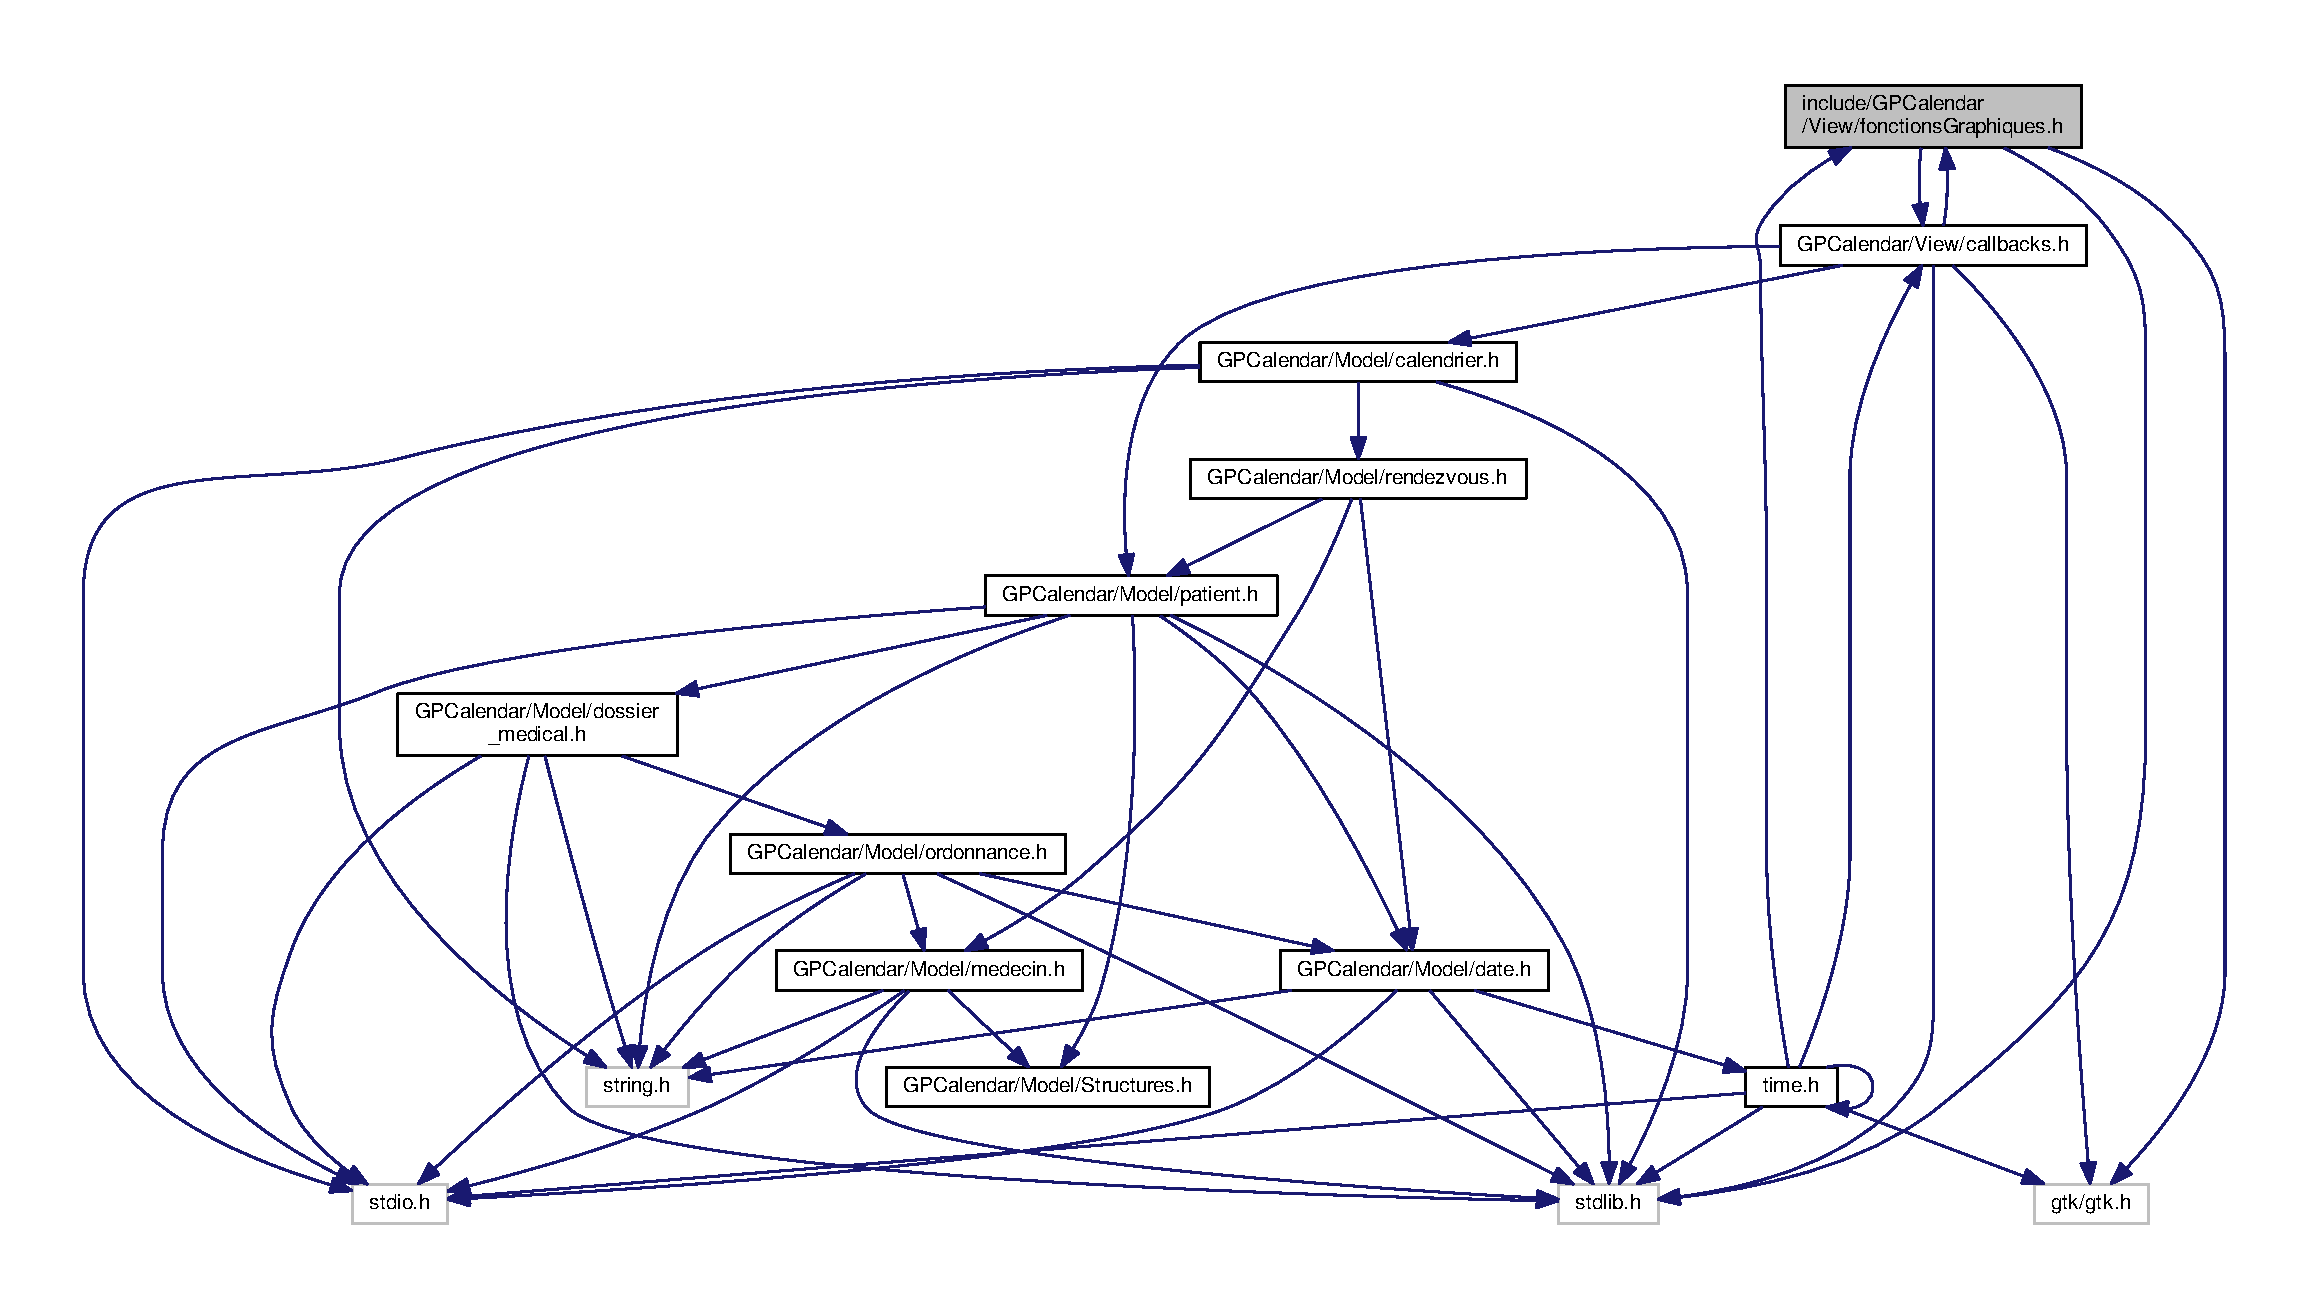
\includegraphics[width=350pt]{fonctions_graphiques_8h__incl}
\end{center}
\end{figure}
Ce graphe montre quels fichiers incluent directement ou indirectement ce fichier \-:
\nopagebreak
\begin{figure}[H]
\begin{center}
\leavevmode
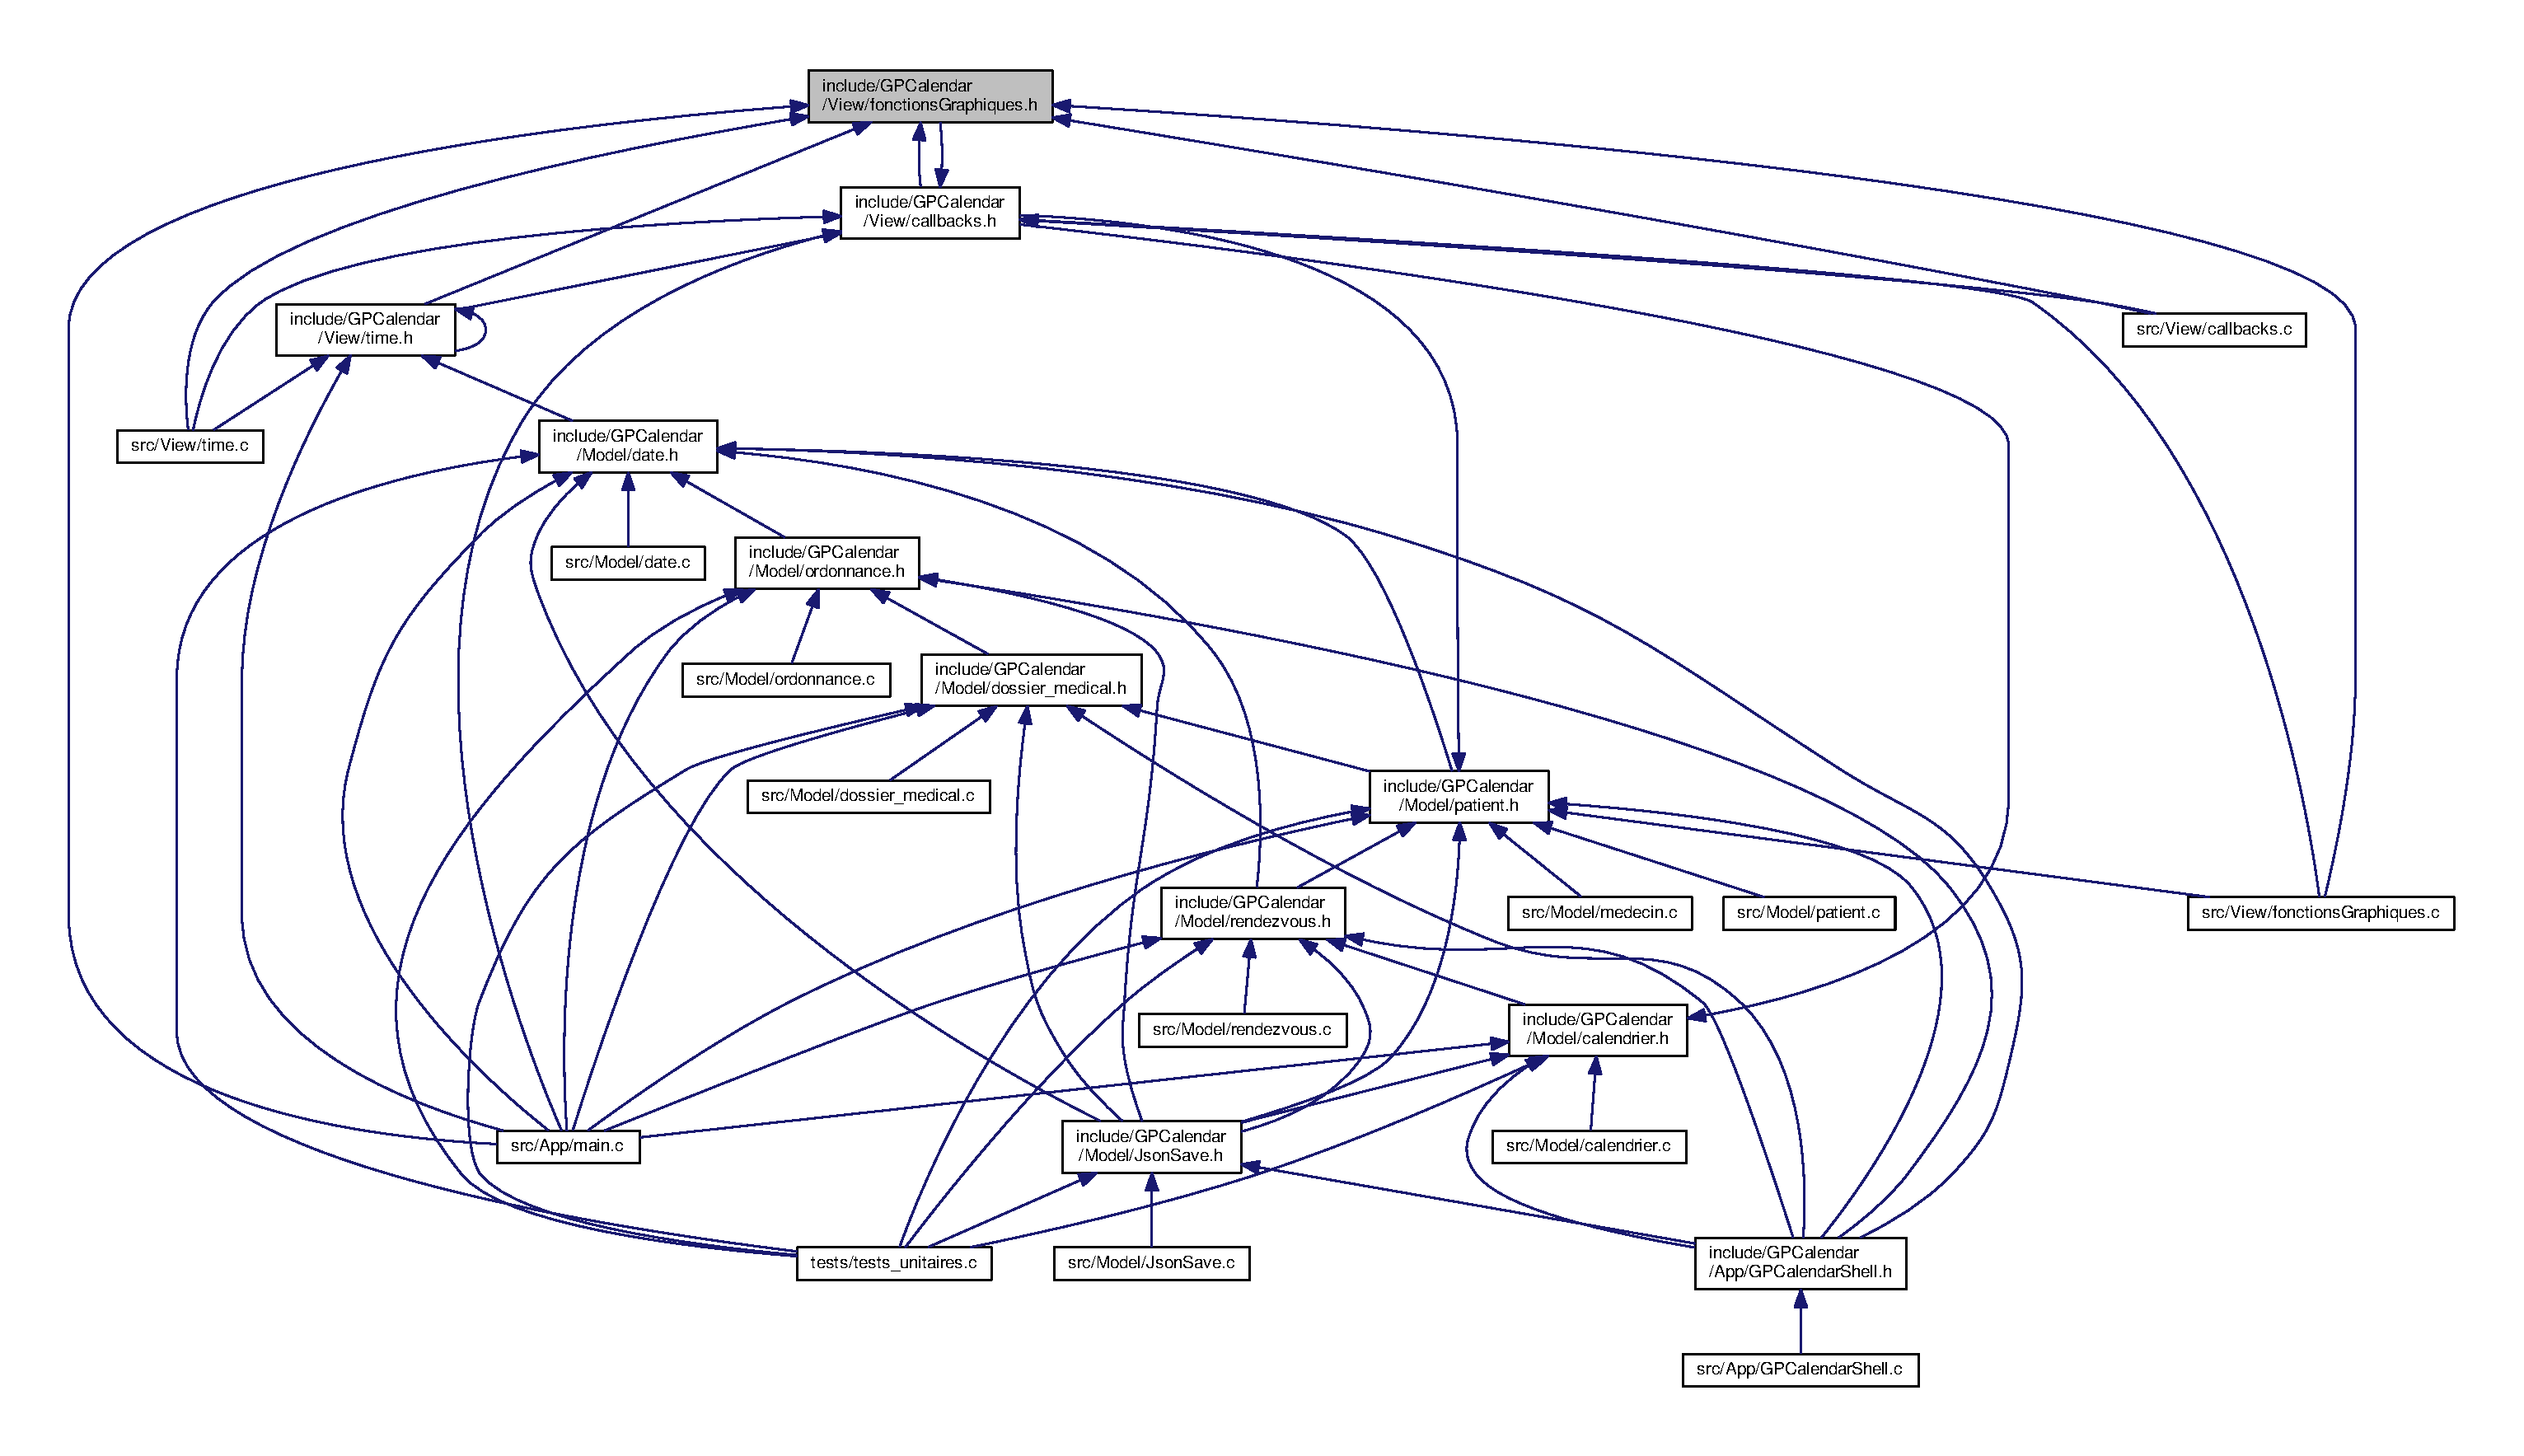
\includegraphics[width=350pt]{fonctions_graphiques_8h__dep__incl}
\end{center}
\end{figure}
\subsection*{Fonctions}
\begin{DoxyCompactItemize}
\item 
int \hyperlink{fonctions_graphiques_8h_a0503e871db78e3e885c9ecd7a5cfbbcf}{create\-\_\-window} (int argc, char $\ast$argv\mbox{[}$\,$\mbox{]})
\item 
void \hyperlink{fonctions_graphiques_8h_a8ca01db52b3fbb75e9632ff6dc724a50}{bouton\-R\-D\-V} (Gtk\-Widget $\ast$wid, Gtk\-Grid grid)
\item 
void \hyperlink{fonctions_graphiques_8h_a75501679d12a0842dbdc6194358f97d7}{parcours\-Jour} (\hyperlink{calendrier_8h_a99e50633bb5c551d09693a390acd33d1}{Jour} j)
\item 
void \hyperlink{fonctions_graphiques_8h_af9da0b3c4675cb9a0cbb0e09e154bb80}{creer\-Bouton\-R\-D\-V} (Gtk\-Widget $\ast$bouton, \hyperlink{struct_rendez_vous}{Rendez\-Vous} $\ast$rdv)
\item 
void \hyperlink{fonctions_graphiques_8h_a081c88af684f01079fb65d79a6d9ae87}{fenetre\-Recherche\-Patient} (Gtk\-Widget $\ast$widget, gpointer data)
\item 
void \hyperlink{fonctions_graphiques_8h_aaa8afd3fb1c2eef8ad968bf26becc0b4}{fenetre\-Creer\-R\-D\-V} (Gtk\-Widget $\ast$widget, gpointer data)
\item 
void \hyperlink{fonctions_graphiques_8h_a280d9560dd03e3e4dd7d11a0e7542b3e}{fenetre\-Creer\-Patient} (Gtk\-Widget $\ast$widget, gpointer data)
\end{DoxyCompactItemize}


\subsection{Description détaillée}
Provides basic unit testing functions declaration. 

\subsection{Documentation des fonctions}
\hypertarget{fonctions_graphiques_8h_a8ca01db52b3fbb75e9632ff6dc724a50}{\index{fonctions\-Graphiques.\-h@{fonctions\-Graphiques.\-h}!bouton\-R\-D\-V@{bouton\-R\-D\-V}}
\index{bouton\-R\-D\-V@{bouton\-R\-D\-V}!fonctionsGraphiques.h@{fonctions\-Graphiques.\-h}}
\subsubsection[{bouton\-R\-D\-V}]{\setlength{\rightskip}{0pt plus 5cm}void bouton\-R\-D\-V (
\begin{DoxyParamCaption}
\item[{Gtk\-Widget $\ast$}]{wid, }
\item[{Gtk\-Grid}]{grid}
\end{DoxyParamCaption}
)}}\label{fonctions_graphiques_8h_a8ca01db52b3fbb75e9632ff6dc724a50}
\hypertarget{fonctions_graphiques_8h_a0503e871db78e3e885c9ecd7a5cfbbcf}{\index{fonctions\-Graphiques.\-h@{fonctions\-Graphiques.\-h}!create\-\_\-window@{create\-\_\-window}}
\index{create\-\_\-window@{create\-\_\-window}!fonctionsGraphiques.h@{fonctions\-Graphiques.\-h}}
\subsubsection[{create\-\_\-window}]{\setlength{\rightskip}{0pt plus 5cm}int create\-\_\-window (
\begin{DoxyParamCaption}
\item[{int}]{argc, }
\item[{char $\ast$}]{argv\mbox{[}$\,$\mbox{]}}
\end{DoxyParamCaption}
)}}\label{fonctions_graphiques_8h_a0503e871db78e3e885c9ecd7a5cfbbcf}
\hypertarget{fonctions_graphiques_8h_af9da0b3c4675cb9a0cbb0e09e154bb80}{\index{fonctions\-Graphiques.\-h@{fonctions\-Graphiques.\-h}!creer\-Bouton\-R\-D\-V@{creer\-Bouton\-R\-D\-V}}
\index{creer\-Bouton\-R\-D\-V@{creer\-Bouton\-R\-D\-V}!fonctionsGraphiques.h@{fonctions\-Graphiques.\-h}}
\subsubsection[{creer\-Bouton\-R\-D\-V}]{\setlength{\rightskip}{0pt plus 5cm}void creer\-Bouton\-R\-D\-V (
\begin{DoxyParamCaption}
\item[{Gtk\-Widget $\ast$}]{bouton, }
\item[{{\bf Rendez\-Vous} $\ast$}]{rdv}
\end{DoxyParamCaption}
)}}\label{fonctions_graphiques_8h_af9da0b3c4675cb9a0cbb0e09e154bb80}
creer\-Bouton\-R\-D\-V \-: associe un bouton du calendrier au patient reçu lors du rendez-\/vous 
\begin{DoxyParams}{Paramètres}
{\em bouton} & \-: le bouton affiché \\
\hline
{\em rdv} & \-: le rendez-\/vous dont on veut associer le patient \\
\hline
\end{DoxyParams}
\hypertarget{fonctions_graphiques_8h_a280d9560dd03e3e4dd7d11a0e7542b3e}{\index{fonctions\-Graphiques.\-h@{fonctions\-Graphiques.\-h}!fenetre\-Creer\-Patient@{fenetre\-Creer\-Patient}}
\index{fenetre\-Creer\-Patient@{fenetre\-Creer\-Patient}!fonctionsGraphiques.h@{fonctions\-Graphiques.\-h}}
\subsubsection[{fenetre\-Creer\-Patient}]{\setlength{\rightskip}{0pt plus 5cm}void fenetre\-Creer\-Patient (
\begin{DoxyParamCaption}
\item[{Gtk\-Widget $\ast$}]{widget, }
\item[{gpointer}]{data}
\end{DoxyParamCaption}
)}}\label{fonctions_graphiques_8h_a280d9560dd03e3e4dd7d11a0e7542b3e}
\hypertarget{fonctions_graphiques_8h_aaa8afd3fb1c2eef8ad968bf26becc0b4}{\index{fonctions\-Graphiques.\-h@{fonctions\-Graphiques.\-h}!fenetre\-Creer\-R\-D\-V@{fenetre\-Creer\-R\-D\-V}}
\index{fenetre\-Creer\-R\-D\-V@{fenetre\-Creer\-R\-D\-V}!fonctionsGraphiques.h@{fonctions\-Graphiques.\-h}}
\subsubsection[{fenetre\-Creer\-R\-D\-V}]{\setlength{\rightskip}{0pt plus 5cm}void fenetre\-Creer\-R\-D\-V (
\begin{DoxyParamCaption}
\item[{Gtk\-Widget $\ast$}]{widget, }
\item[{gpointer}]{data}
\end{DoxyParamCaption}
)}}\label{fonctions_graphiques_8h_aaa8afd3fb1c2eef8ad968bf26becc0b4}
\hypertarget{fonctions_graphiques_8h_a081c88af684f01079fb65d79a6d9ae87}{\index{fonctions\-Graphiques.\-h@{fonctions\-Graphiques.\-h}!fenetre\-Recherche\-Patient@{fenetre\-Recherche\-Patient}}
\index{fenetre\-Recherche\-Patient@{fenetre\-Recherche\-Patient}!fonctionsGraphiques.h@{fonctions\-Graphiques.\-h}}
\subsubsection[{fenetre\-Recherche\-Patient}]{\setlength{\rightskip}{0pt plus 5cm}void fenetre\-Recherche\-Patient (
\begin{DoxyParamCaption}
\item[{Gtk\-Widget $\ast$}]{widget, }
\item[{gpointer}]{data}
\end{DoxyParamCaption}
)}}\label{fonctions_graphiques_8h_a081c88af684f01079fb65d79a6d9ae87}
\hypertarget{fonctions_graphiques_8h_a75501679d12a0842dbdc6194358f97d7}{\index{fonctions\-Graphiques.\-h@{fonctions\-Graphiques.\-h}!parcours\-Jour@{parcours\-Jour}}
\index{parcours\-Jour@{parcours\-Jour}!fonctionsGraphiques.h@{fonctions\-Graphiques.\-h}}
\subsubsection[{parcours\-Jour}]{\setlength{\rightskip}{0pt plus 5cm}void parcours\-Jour (
\begin{DoxyParamCaption}
\item[{{\bf Jour}}]{j}
\end{DoxyParamCaption}
)}}\label{fonctions_graphiques_8h_a75501679d12a0842dbdc6194358f97d7}
parcours\-Jour \-: Parcourir le jour en paramètre et créer un bouton associé à chaque rendez-\/vous 
\begin{DoxyParams}{Paramètres}
{\em j} & \-: le jour (liste de rendez-\/vous) parcouru \\
\hline
\end{DoxyParams}

\hypertarget{time_8h}{\section{Référence du fichier include/\-G\-P\-Calendar/\-View/time.h}
\label{time_8h}\index{include/\-G\-P\-Calendar/\-View/time.\-h@{include/\-G\-P\-Calendar/\-View/time.\-h}}
}
{\ttfamily \#include \char`\"{}G\-P\-Calendar/\-View/fonctions\-Graphiques.\-h\char`\"{}}\\*
{\ttfamily \#include \char`\"{}G\-P\-Calendar/\-View/callbacks.\-h\char`\"{}}\\*
{\ttfamily \#include $<$gtk/gtk.\-h$>$}\\*
{\ttfamily \#include $<$stdlib.\-h$>$}\\*
{\ttfamily \#include $<$stdio.\-h$>$}\\*
{\ttfamily \#include $<$time.\-h$>$}\\*
Graphe des dépendances par inclusion de time.\-h\-:
\nopagebreak
\begin{figure}[H]
\begin{center}
\leavevmode
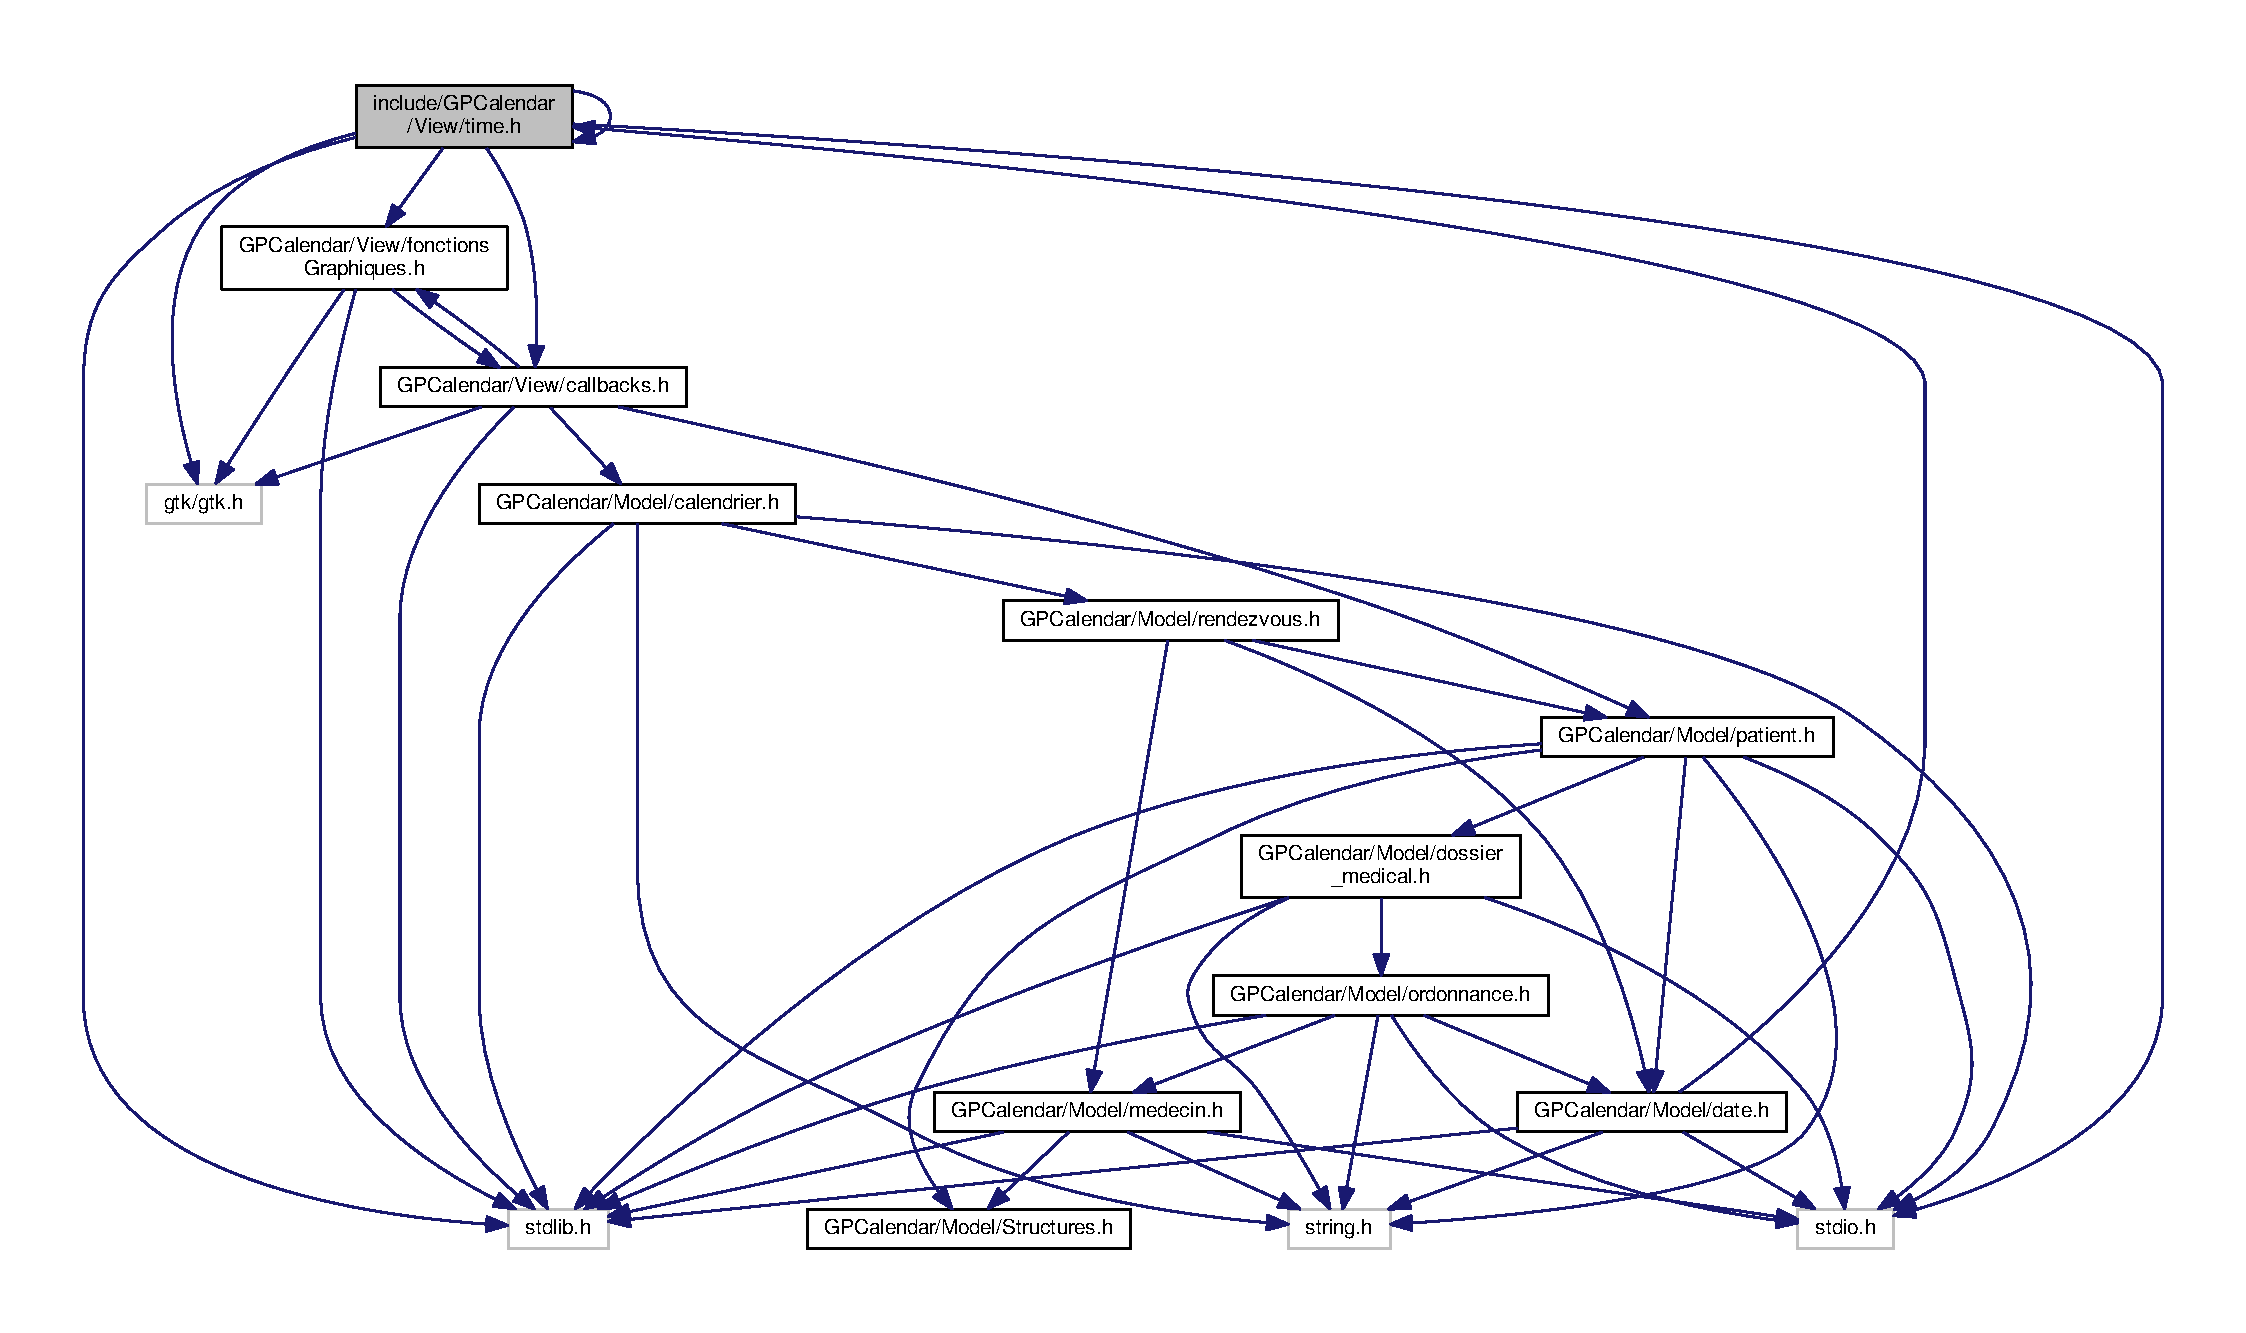
\includegraphics[width=350pt]{time_8h__incl}
\end{center}
\end{figure}
Ce graphe montre quels fichiers incluent directement ou indirectement ce fichier \-:
\nopagebreak
\begin{figure}[H]
\begin{center}
\leavevmode
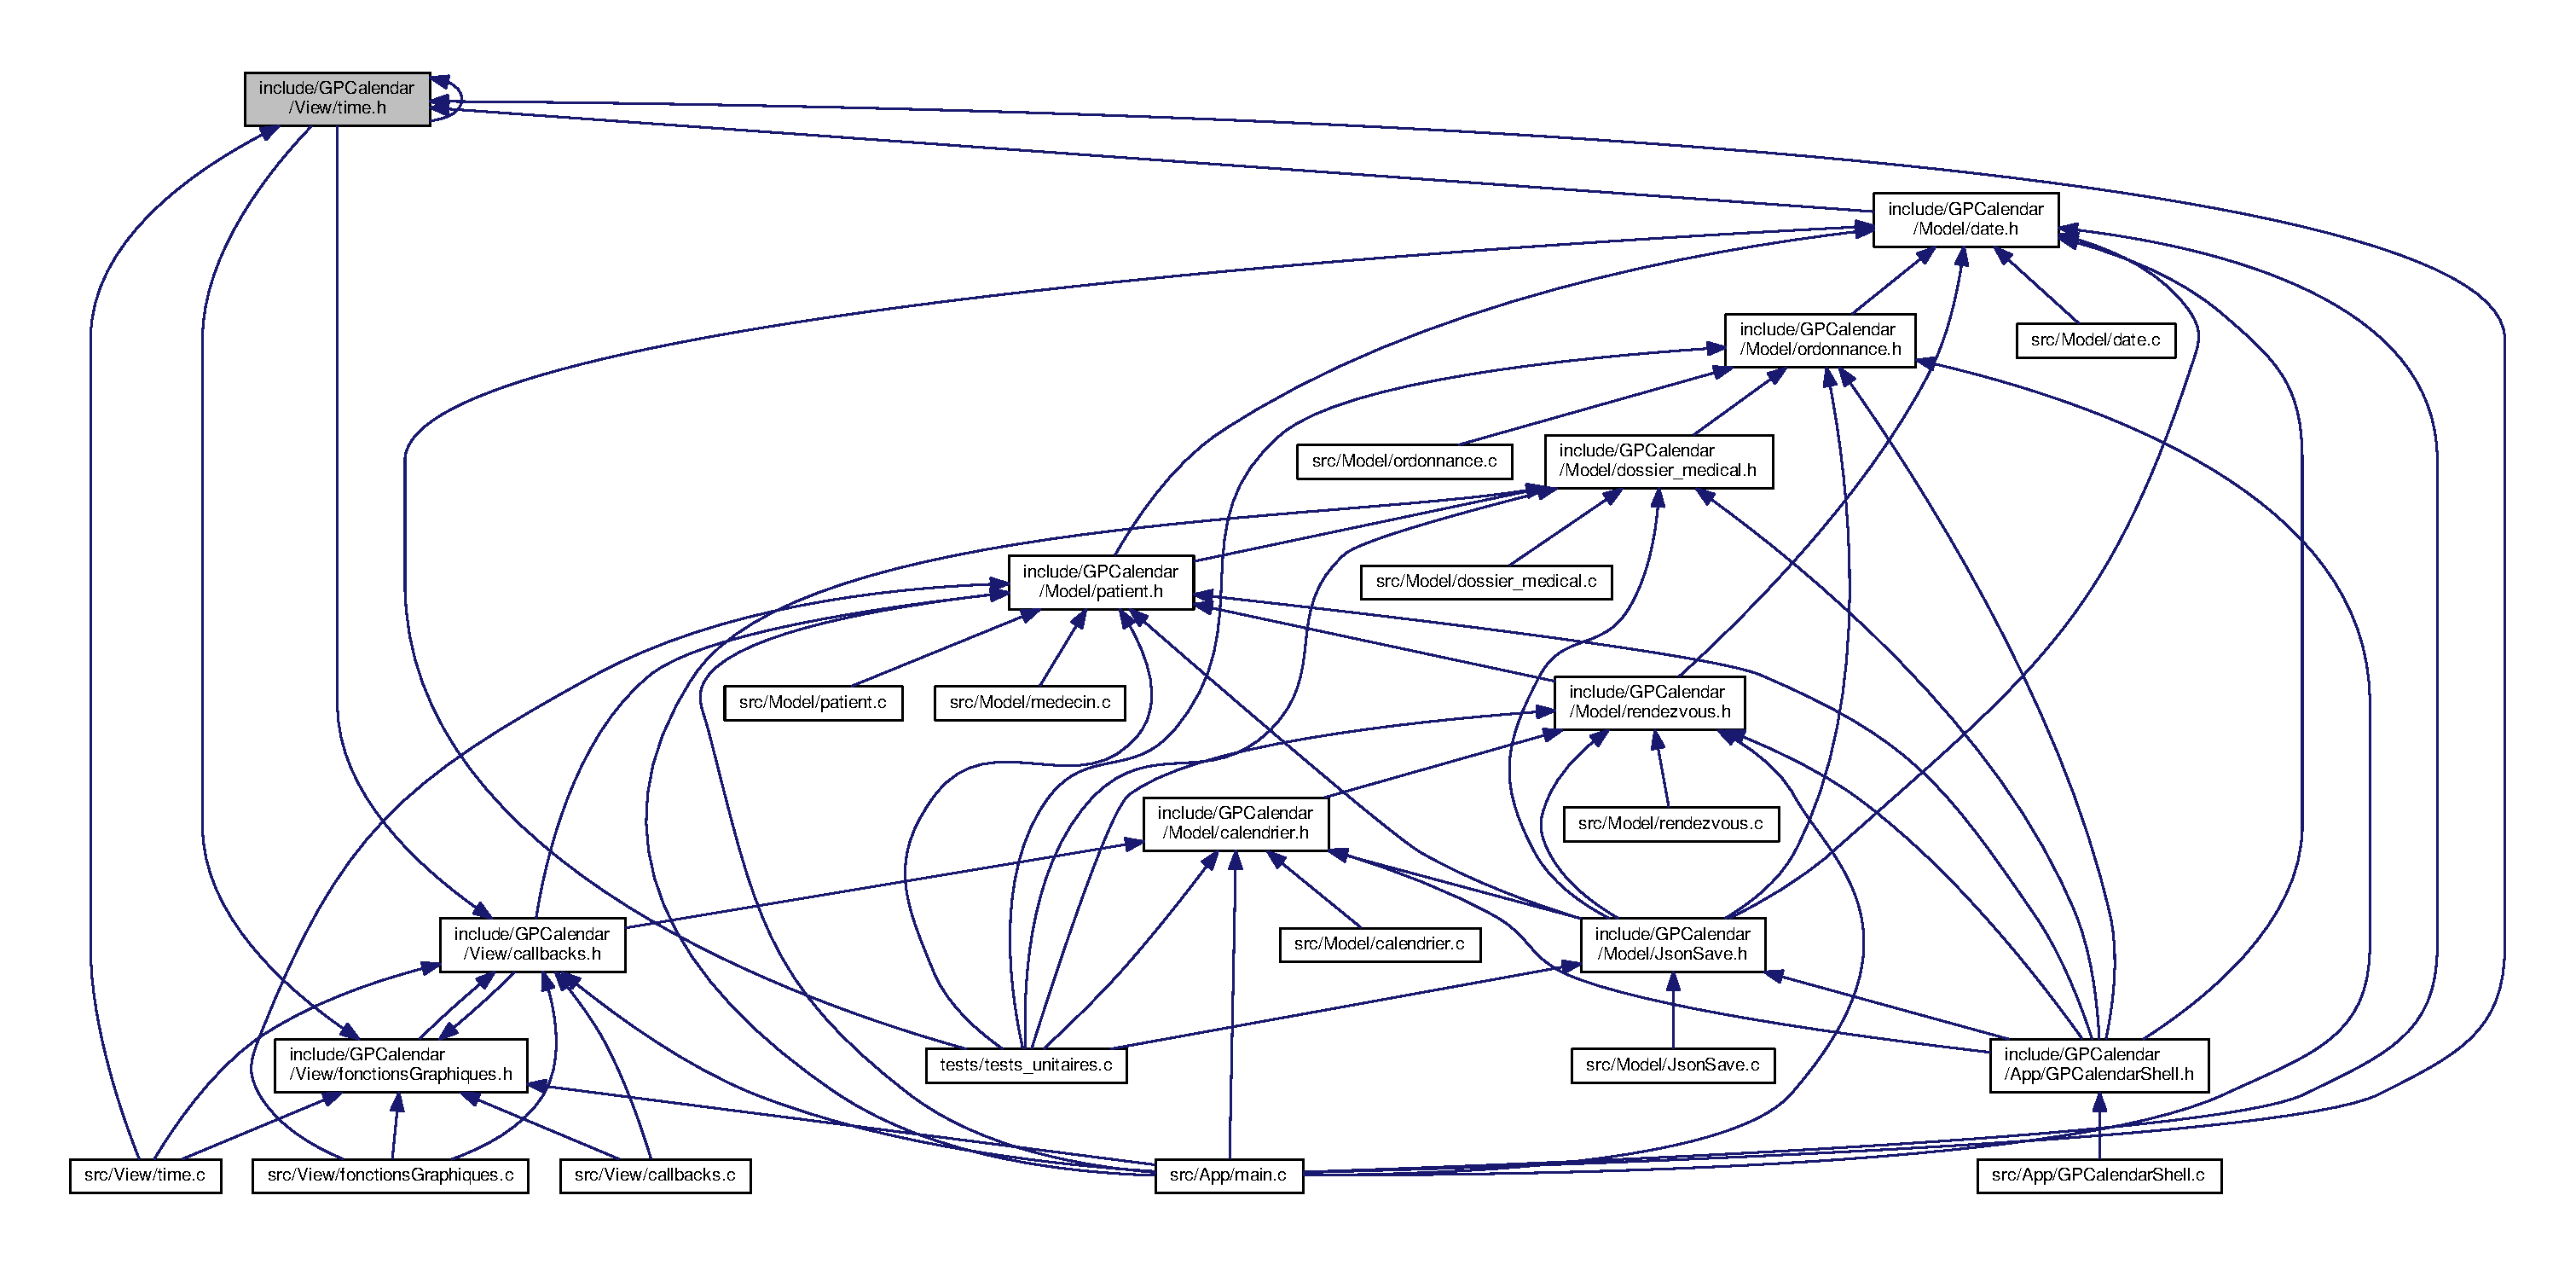
\includegraphics[width=350pt]{time_8h__dep__incl}
\end{center}
\end{figure}
\subsection*{Fonctions}
\begin{DoxyCompactItemize}
\item 
void \hyperlink{time_8h_acc9587936b62ffafdb4a7b283e546ac8}{create\-\_\-calendar} ()
\end{DoxyCompactItemize}


\subsection{Documentation des fonctions}
\hypertarget{time_8h_acc9587936b62ffafdb4a7b283e546ac8}{\index{time.\-h@{time.\-h}!create\-\_\-calendar@{create\-\_\-calendar}}
\index{create\-\_\-calendar@{create\-\_\-calendar}!time.h@{time.\-h}}
\subsubsection[{create\-\_\-calendar}]{\setlength{\rightskip}{0pt plus 5cm}void create\-\_\-calendar (
\begin{DoxyParamCaption}
{}
\end{DoxyParamCaption}
)}}\label{time_8h_acc9587936b62ffafdb4a7b283e546ac8}
create Calendar function 
\hypertarget{_g_p_calendar_shell_8c}{\section{Référence du fichier src/\-App/\-G\-P\-Calendar\-Shell.c}
\label{_g_p_calendar_shell_8c}\index{src/\-App/\-G\-P\-Calendar\-Shell.\-c@{src/\-App/\-G\-P\-Calendar\-Shell.\-c}}
}
{\ttfamily \#include \char`\"{}G\-P\-Calendar\-Shell.\-h\char`\"{}}\\*
Graphe des dépendances par inclusion de G\-P\-Calendar\-Shell.\-c\-:
\nopagebreak
\begin{figure}[H]
\begin{center}
\leavevmode
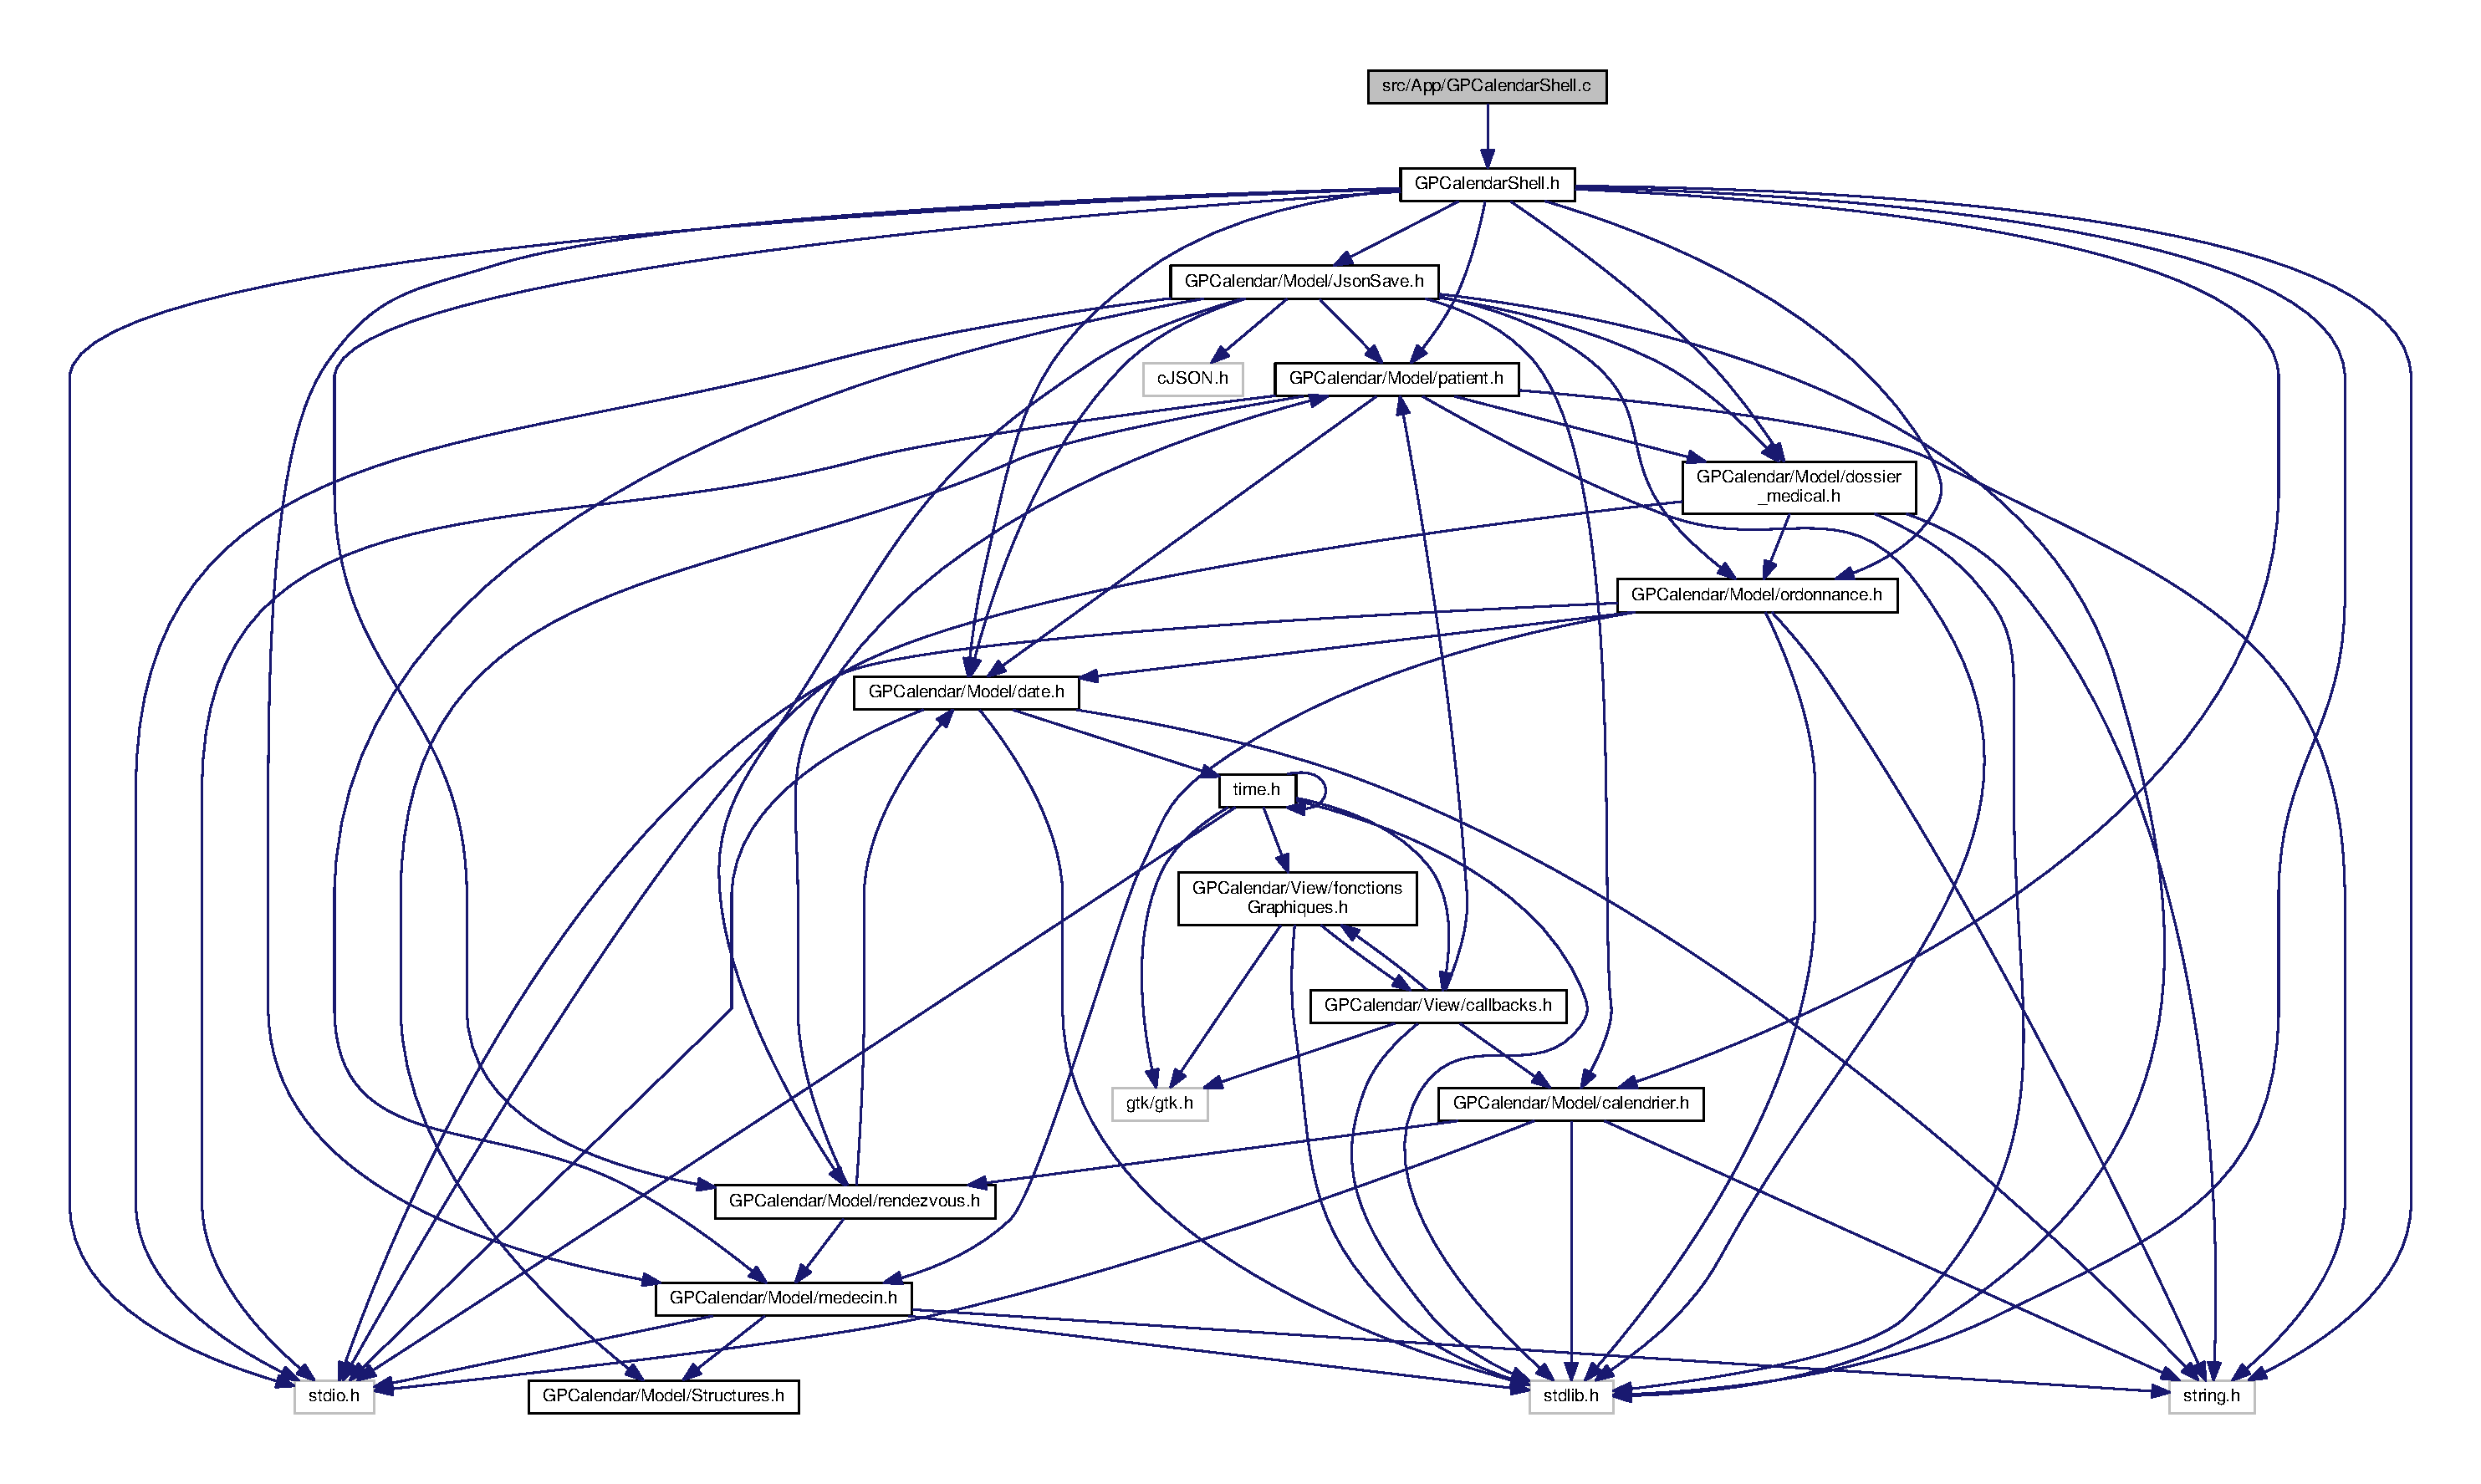
\includegraphics[width=350pt]{_g_p_calendar_shell_8c__incl}
\end{center}
\end{figure}
\subsection*{Fonctions}
\begin{DoxyCompactItemize}
\item 
void \hyperlink{_g_p_calendar_shell_8c_aeb5ca1f06d1f2130fd3df595b9099d3e}{print\-Possible\-Action} ()
\item 
void \hyperlink{_g_p_calendar_shell_8c_adc1f84aaf9010381b234f55a21f7ee27}{Shell\-\_\-creer\-Patient} ()
\item 
void \hyperlink{_g_p_calendar_shell_8c_a4c4a1b40f22e7ba418d1cdd9d112c6a0}{Shell\-\_\-creer\-Medecin} ()
\item 
void \hyperlink{_g_p_calendar_shell_8c_a51b83637c6c6d85cdf3cbf3293de4c5e}{Shell\-\_\-creer\-Rendez\-Vous} ()
\item 
void \hyperlink{_g_p_calendar_shell_8c_adde2df8834cf928dc1575bdd79a319a1}{Shell\-\_\-consulter\-Informations} ()
\item 
void \hyperlink{_g_p_calendar_shell_8c_a9998da37fd86e0715bc3c32a8b03aa75}{Shell\-\_\-annuler\-Rendez\-Vous} ()
\item 
void \hyperlink{_g_p_calendar_shell_8c_a4b5636f1ce8664a9fd3f013974f5e38b}{Shell\-\_\-supprimer\-Patient} ()
\item 
void \hyperlink{_g_p_calendar_shell_8c_adb25a8730eec229efe99eaa5515973fc}{Shell\-\_\-supprimer\-Medecin} ()
\item 
void \hyperlink{_g_p_calendar_shell_8c_af30486979761ada08a0cb4829c382b88}{Shell\-\_\-save\-Project} ()
\item 
void \hyperlink{_g_p_calendar_shell_8c_a5a9b0cab040661b28215cc7d24108141}{Shell\-\_\-load\-Project} ()
\item 
int \hyperlink{_g_p_calendar_shell_8c_a0ddf1224851353fc92bfbff6f499fa97}{main} (int argc, char $\ast$argv\mbox{[}$\,$\mbox{]})
\end{DoxyCompactItemize}


\subsection{Documentation des fonctions}
\hypertarget{_g_p_calendar_shell_8c_a0ddf1224851353fc92bfbff6f499fa97}{\index{G\-P\-Calendar\-Shell.\-c@{G\-P\-Calendar\-Shell.\-c}!main@{main}}
\index{main@{main}!GPCalendarShell.c@{G\-P\-Calendar\-Shell.\-c}}
\subsubsection[{main}]{\setlength{\rightskip}{0pt plus 5cm}int main (
\begin{DoxyParamCaption}
\item[{int}]{argc, }
\item[{char $\ast$}]{argv\mbox{[}$\,$\mbox{]}}
\end{DoxyParamCaption}
)}}\label{_g_p_calendar_shell_8c_a0ddf1224851353fc92bfbff6f499fa97}
Idées d'amélioration \-:
\begin{DoxyItemize}
\item mettre de la couleur (pour les questions ou autres pour différencier les print de ce main ou les print des fonctions appellées)
\item implémenter un \char`\"{}help\char`\"{}
\item 
\end{DoxyItemize}

Demande de l'action à l'utilisateur (utilisation de fgets et strtol)

Switch case pour appeller la fonction correspondant à l'action demandée

On demande à l'utilisateur si il veut continuer à utiliser l'appli \-:
\begin{DoxyItemize}
\item \char`\"{}yes\char`\"{} pour continuer
\begin{DoxyItemize}
\item \char`\"{}no\char`\"{} pour arreter
\end{DoxyItemize}
\end{DoxyItemize}\hypertarget{_g_p_calendar_shell_8c_aeb5ca1f06d1f2130fd3df595b9099d3e}{\index{G\-P\-Calendar\-Shell.\-c@{G\-P\-Calendar\-Shell.\-c}!print\-Possible\-Action@{print\-Possible\-Action}}
\index{print\-Possible\-Action@{print\-Possible\-Action}!GPCalendarShell.c@{G\-P\-Calendar\-Shell.\-c}}
\subsubsection[{print\-Possible\-Action}]{\setlength{\rightskip}{0pt plus 5cm}void print\-Possible\-Action (
\begin{DoxyParamCaption}
{}
\end{DoxyParamCaption}
)}}\label{_g_p_calendar_shell_8c_aeb5ca1f06d1f2130fd3df595b9099d3e}
\hypertarget{_g_p_calendar_shell_8c_a9998da37fd86e0715bc3c32a8b03aa75}{\index{G\-P\-Calendar\-Shell.\-c@{G\-P\-Calendar\-Shell.\-c}!Shell\-\_\-annuler\-Rendez\-Vous@{Shell\-\_\-annuler\-Rendez\-Vous}}
\index{Shell\-\_\-annuler\-Rendez\-Vous@{Shell\-\_\-annuler\-Rendez\-Vous}!GPCalendarShell.c@{G\-P\-Calendar\-Shell.\-c}}
\subsubsection[{Shell\-\_\-annuler\-Rendez\-Vous}]{\setlength{\rightskip}{0pt plus 5cm}void Shell\-\_\-annuler\-Rendez\-Vous (
\begin{DoxyParamCaption}
{}
\end{DoxyParamCaption}
)}}\label{_g_p_calendar_shell_8c_a9998da37fd86e0715bc3c32a8b03aa75}
\hypertarget{_g_p_calendar_shell_8c_adde2df8834cf928dc1575bdd79a319a1}{\index{G\-P\-Calendar\-Shell.\-c@{G\-P\-Calendar\-Shell.\-c}!Shell\-\_\-consulter\-Informations@{Shell\-\_\-consulter\-Informations}}
\index{Shell\-\_\-consulter\-Informations@{Shell\-\_\-consulter\-Informations}!GPCalendarShell.c@{G\-P\-Calendar\-Shell.\-c}}
\subsubsection[{Shell\-\_\-consulter\-Informations}]{\setlength{\rightskip}{0pt plus 5cm}void Shell\-\_\-consulter\-Informations (
\begin{DoxyParamCaption}
{}
\end{DoxyParamCaption}
)}}\label{_g_p_calendar_shell_8c_adde2df8834cf928dc1575bdd79a319a1}
\hypertarget{_g_p_calendar_shell_8c_a4c4a1b40f22e7ba418d1cdd9d112c6a0}{\index{G\-P\-Calendar\-Shell.\-c@{G\-P\-Calendar\-Shell.\-c}!Shell\-\_\-creer\-Medecin@{Shell\-\_\-creer\-Medecin}}
\index{Shell\-\_\-creer\-Medecin@{Shell\-\_\-creer\-Medecin}!GPCalendarShell.c@{G\-P\-Calendar\-Shell.\-c}}
\subsubsection[{Shell\-\_\-creer\-Medecin}]{\setlength{\rightskip}{0pt plus 5cm}void Shell\-\_\-creer\-Medecin (
\begin{DoxyParamCaption}
{}
\end{DoxyParamCaption}
)}}\label{_g_p_calendar_shell_8c_a4c4a1b40f22e7ba418d1cdd9d112c6a0}
\hypertarget{_g_p_calendar_shell_8c_adc1f84aaf9010381b234f55a21f7ee27}{\index{G\-P\-Calendar\-Shell.\-c@{G\-P\-Calendar\-Shell.\-c}!Shell\-\_\-creer\-Patient@{Shell\-\_\-creer\-Patient}}
\index{Shell\-\_\-creer\-Patient@{Shell\-\_\-creer\-Patient}!GPCalendarShell.c@{G\-P\-Calendar\-Shell.\-c}}
\subsubsection[{Shell\-\_\-creer\-Patient}]{\setlength{\rightskip}{0pt plus 5cm}void Shell\-\_\-creer\-Patient (
\begin{DoxyParamCaption}
{}
\end{DoxyParamCaption}
)}}\label{_g_p_calendar_shell_8c_adc1f84aaf9010381b234f55a21f7ee27}
\hypertarget{_g_p_calendar_shell_8c_a51b83637c6c6d85cdf3cbf3293de4c5e}{\index{G\-P\-Calendar\-Shell.\-c@{G\-P\-Calendar\-Shell.\-c}!Shell\-\_\-creer\-Rendez\-Vous@{Shell\-\_\-creer\-Rendez\-Vous}}
\index{Shell\-\_\-creer\-Rendez\-Vous@{Shell\-\_\-creer\-Rendez\-Vous}!GPCalendarShell.c@{G\-P\-Calendar\-Shell.\-c}}
\subsubsection[{Shell\-\_\-creer\-Rendez\-Vous}]{\setlength{\rightskip}{0pt plus 5cm}void Shell\-\_\-creer\-Rendez\-Vous (
\begin{DoxyParamCaption}
{}
\end{DoxyParamCaption}
)}}\label{_g_p_calendar_shell_8c_a51b83637c6c6d85cdf3cbf3293de4c5e}
\hypertarget{_g_p_calendar_shell_8c_a5a9b0cab040661b28215cc7d24108141}{\index{G\-P\-Calendar\-Shell.\-c@{G\-P\-Calendar\-Shell.\-c}!Shell\-\_\-load\-Project@{Shell\-\_\-load\-Project}}
\index{Shell\-\_\-load\-Project@{Shell\-\_\-load\-Project}!GPCalendarShell.c@{G\-P\-Calendar\-Shell.\-c}}
\subsubsection[{Shell\-\_\-load\-Project}]{\setlength{\rightskip}{0pt plus 5cm}void Shell\-\_\-load\-Project (
\begin{DoxyParamCaption}
{}
\end{DoxyParamCaption}
)}}\label{_g_p_calendar_shell_8c_a5a9b0cab040661b28215cc7d24108141}
\hypertarget{_g_p_calendar_shell_8c_af30486979761ada08a0cb4829c382b88}{\index{G\-P\-Calendar\-Shell.\-c@{G\-P\-Calendar\-Shell.\-c}!Shell\-\_\-save\-Project@{Shell\-\_\-save\-Project}}
\index{Shell\-\_\-save\-Project@{Shell\-\_\-save\-Project}!GPCalendarShell.c@{G\-P\-Calendar\-Shell.\-c}}
\subsubsection[{Shell\-\_\-save\-Project}]{\setlength{\rightskip}{0pt plus 5cm}void Shell\-\_\-save\-Project (
\begin{DoxyParamCaption}
{}
\end{DoxyParamCaption}
)}}\label{_g_p_calendar_shell_8c_af30486979761ada08a0cb4829c382b88}
\hypertarget{_g_p_calendar_shell_8c_adb25a8730eec229efe99eaa5515973fc}{\index{G\-P\-Calendar\-Shell.\-c@{G\-P\-Calendar\-Shell.\-c}!Shell\-\_\-supprimer\-Medecin@{Shell\-\_\-supprimer\-Medecin}}
\index{Shell\-\_\-supprimer\-Medecin@{Shell\-\_\-supprimer\-Medecin}!GPCalendarShell.c@{G\-P\-Calendar\-Shell.\-c}}
\subsubsection[{Shell\-\_\-supprimer\-Medecin}]{\setlength{\rightskip}{0pt plus 5cm}void Shell\-\_\-supprimer\-Medecin (
\begin{DoxyParamCaption}
{}
\end{DoxyParamCaption}
)}}\label{_g_p_calendar_shell_8c_adb25a8730eec229efe99eaa5515973fc}
\hypertarget{_g_p_calendar_shell_8c_a4b5636f1ce8664a9fd3f013974f5e38b}{\index{G\-P\-Calendar\-Shell.\-c@{G\-P\-Calendar\-Shell.\-c}!Shell\-\_\-supprimer\-Patient@{Shell\-\_\-supprimer\-Patient}}
\index{Shell\-\_\-supprimer\-Patient@{Shell\-\_\-supprimer\-Patient}!GPCalendarShell.c@{G\-P\-Calendar\-Shell.\-c}}
\subsubsection[{Shell\-\_\-supprimer\-Patient}]{\setlength{\rightskip}{0pt plus 5cm}void Shell\-\_\-supprimer\-Patient (
\begin{DoxyParamCaption}
{}
\end{DoxyParamCaption}
)}}\label{_g_p_calendar_shell_8c_a4b5636f1ce8664a9fd3f013974f5e38b}

\hypertarget{main_8c}{\section{Référence du fichier src/\-App/main.c}
\label{main_8c}\index{src/\-App/main.\-c@{src/\-App/main.\-c}}
}
{\ttfamily \#include \char`\"{}G\-P\-Calendar/\-Model/medecin.\-h\char`\"{}}\\*
{\ttfamily \#include \char`\"{}G\-P\-Calendar/\-Model/patient.\-h\char`\"{}}\\*
{\ttfamily \#include \char`\"{}G\-P\-Calendar/\-Model/date.\-h\char`\"{}}\\*
{\ttfamily \#include \char`\"{}G\-P\-Calendar/\-Model/calendrier.\-h\char`\"{}}\\*
{\ttfamily \#include \char`\"{}G\-P\-Calendar/\-Model/ordonnance.\-h\char`\"{}}\\*
{\ttfamily \#include \char`\"{}G\-P\-Calendar/\-Model/dossier\-\_\-medical.\-h\char`\"{}}\\*
{\ttfamily \#include \char`\"{}G\-P\-Calendar/\-Model/rendezvous.\-h\char`\"{}}\\*
{\ttfamily \#include \char`\"{}G\-P\-Calendar/\-View/fonctions\-Graphiques.\-h\char`\"{}}\\*
{\ttfamily \#include \char`\"{}G\-P\-Calendar/\-View/callbacks.\-h\char`\"{}}\\*
{\ttfamily \#include \char`\"{}G\-P\-Calendar/\-View/time.\-h\char`\"{}}\\*
{\ttfamily \#include $<$gtk/gtk.\-h$>$}\\*
{\ttfamily \#include $<$string.\-h$>$}\\*
{\ttfamily \#include $<$stdio.\-h$>$}\\*
{\ttfamily \#include $<$stdlib.\-h$>$}\\*
Graphe des dépendances par inclusion de main.\-c\-:
\nopagebreak
\begin{figure}[H]
\begin{center}
\leavevmode
\includegraphics[width=350pt]{main_8c__incl}
\end{center}
\end{figure}
\subsection*{Fonctions}
\begin{DoxyCompactItemize}
\item 
int \hyperlink{main_8c_a0ddf1224851353fc92bfbff6f499fa97}{main} (int argc, char $\ast$argv\mbox{[}$\,$\mbox{]})
\end{DoxyCompactItemize}


\subsection{Documentation des fonctions}
\hypertarget{main_8c_a0ddf1224851353fc92bfbff6f499fa97}{\index{main.\-c@{main.\-c}!main@{main}}
\index{main@{main}!main.c@{main.\-c}}
\subsubsection[{main}]{\setlength{\rightskip}{0pt plus 5cm}int main (
\begin{DoxyParamCaption}
\item[{int}]{argc, }
\item[{char $\ast$}]{argv\mbox{[}$\,$\mbox{]}}
\end{DoxyParamCaption}
)}}\label{main_8c_a0ddf1224851353fc92bfbff6f499fa97}
1 -\/ Récupération des listes de patients et de mèdecins existants (On les appellera un truc comme Registered\-Patient/\-Medecin)

2 -\/ Récupération du ou des Calendriers (dépendra de la version, pour la V0 c'est du \-: le calendrier de l'hopital)

3 -\/ Un petit print dans G\-T\-K et la console pour voir le fichier I\-S\-C qu'on à load

Inscription de nouveaux patients / mèdecins Création de nouveaux rdv / ordonnances et maj du calendrier Lecture d'infos persos de \hyperlink{struct_patient}{Patient} / Medecins etc ...

1 -\/ Demande à l'utilisateur si il veut save ses données dans un fichier I\-S\-C, si oui bah le faire

2 -\/ Après avoir save, free tout les objets load en mémoire après l'ouverture et l'utilisation de l'appli

3 -\/ Fermer G\-T\-K
\hypertarget{calendrier_8c}{\section{Référence du fichier src/\-Model/calendrier.c}
\label{calendrier_8c}\index{src/\-Model/calendrier.\-c@{src/\-Model/calendrier.\-c}}
}
{\ttfamily \#include \char`\"{}G\-P\-Calendar/\-Model/calendrier.\-h\char`\"{}}\\*
Graphe des dépendances par inclusion de calendrier.\-c\-:
\nopagebreak
\begin{figure}[H]
\begin{center}
\leavevmode
\includegraphics[width=350pt]{calendrier_8c__incl}
\end{center}
\end{figure}
\subsection*{Fonctions}
\begin{DoxyCompactItemize}
\item 
int \hyperlink{calendrier_8c_af5442fe73fe43e982dec5ae9b36bd0f2}{Add\-Rendez\-Vous\-\_\-\-Calendrier} (\hyperlink{calendrier_8h_ab8644d1026df84be3eb3190cf1ef29fa}{Calendrier} c, \hyperlink{struct_rendez_vous}{Rendez\-Vous} $\ast$rdv)
\item 
void \hyperlink{calendrier_8c_a58b7e50ba3bf89beb9ad2b77cd83a425}{free\-Calendrier} (\hyperlink{calendrier_8h_ab8644d1026df84be3eb3190cf1ef29fa}{Calendrier} c)
\item 
int \hyperlink{calendrier_8c_a5968c63f3b806d8f670fbfd965d755e4}{chercher\-Rendez\-Vous\-\_\-\-Calendrier} (\hyperlink{calendrier_8h_ab8644d1026df84be3eb3190cf1ef29fa}{Calendrier} c, \hyperlink{struct_rendez_vous}{Rendez\-Vous} $\ast$rdv)
\item 
void \hyperlink{calendrier_8c_ac2199296f615dbb3728385f855cc201e}{print\-Calendrier} (\hyperlink{calendrier_8h_ab8644d1026df84be3eb3190cf1ef29fa}{Calendrier} c)
\item 
int \hyperlink{calendrier_8c_a0567b0b4423c3656ac5b969111936626}{Add\-Rendez\-Vous\-\_\-\-Jour} (\hyperlink{calendrier_8h_a99e50633bb5c551d09693a390acd33d1}{Jour} j, \hyperlink{struct_rendez_vous}{Rendez\-Vous} $\ast$rdv)
\item 
int \hyperlink{calendrier_8c_a47b839047989693d1e760e0dd0fa6243}{Chercher\-Rendez\-Vous\-Suivant} (\hyperlink{calendrier_8h_a99e50633bb5c551d09693a390acd33d1}{Jour} j, \hyperlink{struct_rendez_vous}{Rendez\-Vous} $\ast$rdv)
\item 
int \hyperlink{calendrier_8c_a8b99489007274be2dc239cdf8be3c524}{Add\-Jour\-\_\-\-Mois} (\hyperlink{calendrier_8h_ae3a97c3f15c38f94baef498c511b4258}{Mois} m, \hyperlink{calendrier_8h_a99e50633bb5c551d09693a390acd33d1}{Jour} j)
\item 
int \hyperlink{calendrier_8c_ac38aff1a5ce7c90a443c2a8bda6eaad1}{Add\-Mois\-\_\-\-Annee} (\hyperlink{calendrier_8h_a8e119d682702ebf078b3235b4c0fe464}{Annee} a, \hyperlink{calendrier_8h_ae3a97c3f15c38f94baef498c511b4258}{Mois} m)
\item 
int \hyperlink{calendrier_8c_a450576665db3511a8bffd8a3dbade73b}{Add\-Annee\-\_\-\-Calendrier} (\hyperlink{calendrier_8h_ab8644d1026df84be3eb3190cf1ef29fa}{Calendrier} c, \hyperlink{calendrier_8h_a8e119d682702ebf078b3235b4c0fe464}{Annee} a)
\item 
\hyperlink{struct_rendez_vous}{Rendez\-Vous} $\ast$ \hyperlink{calendrier_8c_ab33fde0e75227f51c28053e2d8eae36f}{Rendez\-Vous\-\_\-existe} (\hyperlink{struct_list_rendez_vous}{List\-Rendez\-Vous} $\ast$l, \hyperlink{struct_rendez_vous}{Rendez\-Vous} $\ast$rdv)
\item 
\hyperlink{struct_list_rendez_vous}{List\-Rendez\-Vous} $\ast$ \hyperlink{calendrier_8c_a415ff7b2abfcdcd9aecc18d2a9897d2e}{Jour\-\_\-existe} (\hyperlink{struct_list_jour}{List\-Jour} $\ast$l, \hyperlink{struct_date}{Date} $\ast$d)
\item 
\hyperlink{struct_list_jour}{List\-Jour} $\ast$ \hyperlink{calendrier_8c_a1c5790002b48d96f4057746e974d77e5}{Mois\-\_\-existe} (\hyperlink{struct_list_mois}{List\-Mois} $\ast$l, int mois)
\item 
\hyperlink{struct_list_mois}{List\-Mois} $\ast$ \hyperlink{calendrier_8c_a4b41af28922cc8adef5d829997b74e29}{Annee\-\_\-existe} (\hyperlink{struct_list_annee}{List\-Annee} $\ast$l, int annee)
\item 
\hyperlink{struct_node_rendez_vous}{Node\-Rendez\-Vous} $\ast$ \hyperlink{calendrier_8c_a64191f7428e9d03b0042e91ba8daedda}{new\-Node\-Rendez\-Vous} (\hyperlink{struct_rendez_vous}{Rendez\-Vous} $\ast$rdv, \hyperlink{struct_node_rendez_vous}{Node\-Rendez\-Vous} $\ast$previous, \hyperlink{struct_node_rendez_vous}{Node\-Rendez\-Vous} $\ast$next)
\item 
void \hyperlink{calendrier_8c_a1fbcadf4b456c9bff151fe47f7dab17e}{free\-Node\-Rendez\-Vous} (\hyperlink{struct_list_rendez_vous}{List\-Rendez\-Vous} $\ast$l, \hyperlink{struct_node_rendez_vous}{Node\-Rendez\-Vous} $\ast$n)
\item 
void \hyperlink{calendrier_8c_a23e5ea4de8dba5e7782907621774c881}{List\-Rendez\-Vous\-\_\-init} (\hyperlink{struct_list_rendez_vous}{List\-Rendez\-Vous} $\ast$l, \hyperlink{struct_date}{Date} $\ast$date)
\item 
void \hyperlink{calendrier_8c_aa4a3a8b4abb465a6f161ef09d1c7a7c8}{List\-Rendez\-Vous\-\_\-free} (\hyperlink{struct_list_rendez_vous}{List\-Rendez\-Vous} $\ast$l)
\item 
int \hyperlink{calendrier_8c_a71f6dc0c84a3542f6079487b72d558fb}{List\-Rendez\-Vous\-\_\-is\-Empty} (\hyperlink{struct_list_rendez_vous}{List\-Rendez\-Vous} $\ast$l)
\item 
int \hyperlink{calendrier_8c_ab8555690cee8bc78ce0e8d4bffedf06a}{List\-Rendez\-Vous\-\_\-is\-First} (\hyperlink{struct_list_rendez_vous}{List\-Rendez\-Vous} $\ast$l)
\item 
int \hyperlink{calendrier_8c_a9463e60d5c1910777b37beb5928115f2}{List\-Rendez\-Vous\-\_\-is\-Last} (\hyperlink{struct_list_rendez_vous}{List\-Rendez\-Vous} $\ast$l)
\item 
int \hyperlink{calendrier_8c_afd1dd22d5e4fe7c1c416e6c0f200b308}{List\-Rendez\-Vous\-\_\-is\-Out\-Of\-List} (\hyperlink{struct_list_rendez_vous}{List\-Rendez\-Vous} $\ast$l)
\item 
void \hyperlink{calendrier_8c_a164b598d8b392c7fdbc2cd2de8e43fae}{List\-Rendez\-Vous\-\_\-set\-On\-First} (\hyperlink{struct_list_rendez_vous}{List\-Rendez\-Vous} $\ast$l)
\item 
void \hyperlink{calendrier_8c_a05b8f2671d1ddef046a1dc4585982fdf}{List\-Rendez\-Vous\-\_\-set\-On\-Last} (\hyperlink{struct_list_rendez_vous}{List\-Rendez\-Vous} $\ast$l)
\item 
void \hyperlink{calendrier_8c_ad4b835cfb870b007a3b9cae580ca673a}{List\-Rendez\-Vous\-\_\-set\-On\-Next} (\hyperlink{struct_list_rendez_vous}{List\-Rendez\-Vous} $\ast$l)
\item 
void \hyperlink{calendrier_8c_a65f7c91ca3b63a07b9d67aac2e4ae1a2}{List\-Rendez\-Vous\-\_\-set\-On\-Previous} (\hyperlink{struct_list_rendez_vous}{List\-Rendez\-Vous} $\ast$l)
\item 
\hyperlink{struct_rendez_vous}{Rendez\-Vous} $\ast$ \hyperlink{calendrier_8c_a3f0f57991d4199f6b115e9cfd4416f22}{List\-Rendez\-Vous\-\_\-get\-Current} (\hyperlink{struct_list_rendez_vous}{List\-Rendez\-Vous} $\ast$l)
\item 
\hyperlink{struct_date}{Date} $\ast$ \hyperlink{calendrier_8c_a0e59bdc8c647207f998467ef782ac3e6}{List\-Rendez\-Vous\-\_\-get\-Date} (\hyperlink{struct_list_rendez_vous}{List\-Rendez\-Vous} $\ast$l)
\item 
\hyperlink{struct_node_jour}{Node\-Jour} $\ast$ \hyperlink{calendrier_8c_a239864286dae5eb5fad8d4d1aec8dd61}{new\-Node\-Jour} (\hyperlink{calendrier_8h_a99e50633bb5c551d09693a390acd33d1}{Jour} jour, \hyperlink{struct_node_jour}{Node\-Jour} $\ast$previous, \hyperlink{struct_node_jour}{Node\-Jour} $\ast$next)
\item 
void \hyperlink{calendrier_8c_aa01efc6ea9dcc9c84cbf338eaf6edc0c}{free\-Node\-Jour} (\hyperlink{struct_list_jour}{List\-Jour} $\ast$l, \hyperlink{struct_node_jour}{Node\-Jour} $\ast$n)
\item 
void \hyperlink{calendrier_8c_ad023df59ece4d1364fcd2ca60a324136}{List\-Jour\-\_\-init} (\hyperlink{struct_list_jour}{List\-Jour} $\ast$l, int mois)
\item 
void \hyperlink{calendrier_8c_a6ba8a2ee92a1f19beb9e50f81b0d3eeb}{List\-Jour\-\_\-free} (\hyperlink{struct_list_jour}{List\-Jour} $\ast$l)
\item 
int \hyperlink{calendrier_8c_ac741a3bf9a8d15974d16008c321b5ea1}{List\-Jour\-\_\-is\-Empty} (\hyperlink{struct_list_jour}{List\-Jour} $\ast$l)
\item 
int \hyperlink{calendrier_8c_a4b92599c29997802ffd9c443f0add8be}{List\-Jour\-\_\-is\-First} (\hyperlink{struct_list_jour}{List\-Jour} $\ast$l)
\item 
int \hyperlink{calendrier_8c_a56bfd9c2ae8c423545862af4c98b0e53}{List\-Jour\-\_\-is\-Last} (\hyperlink{struct_list_jour}{List\-Jour} $\ast$l)
\item 
int \hyperlink{calendrier_8c_a128e2f52a208077d8f00584623959436}{List\-Jour\-\_\-is\-Out\-Of\-List} (\hyperlink{struct_list_jour}{List\-Jour} $\ast$l)
\item 
void \hyperlink{calendrier_8c_a141f34ddd47c285e4decf8a43f971edc}{List\-Jour\-\_\-set\-On\-First} (\hyperlink{struct_list_jour}{List\-Jour} $\ast$l)
\item 
void \hyperlink{calendrier_8c_ae898b127aa5450827d488b210abffef7}{List\-Jour\-\_\-set\-On\-Last} (\hyperlink{struct_list_jour}{List\-Jour} $\ast$l)
\item 
void \hyperlink{calendrier_8c_abcf20bcdd09cd93bce93c89683463761}{List\-Jour\-\_\-set\-On\-Next} (\hyperlink{struct_list_jour}{List\-Jour} $\ast$l)
\item 
void \hyperlink{calendrier_8c_a22e61f6532a2ca6e9e0246319605e627}{List\-Jour\-\_\-set\-On\-Previous} (\hyperlink{struct_list_jour}{List\-Jour} $\ast$l)
\item 
\hyperlink{calendrier_8h_a99e50633bb5c551d09693a390acd33d1}{Jour} \hyperlink{calendrier_8c_a7ce754eccbdb2cd861def01a3ba31e46}{List\-Jour\-\_\-get\-Current} (\hyperlink{struct_list_jour}{List\-Jour} $\ast$l)
\item 
int \hyperlink{calendrier_8c_ad7e32f962738c27befaadd9682e85abd}{List\-Jour\-\_\-get\-Mois} (\hyperlink{struct_list_jour}{List\-Jour} $\ast$l)
\item 
\hyperlink{struct_node_mois}{Node\-Mois} $\ast$ \hyperlink{calendrier_8c_a9d1def1692e1773aced0df50e636a497}{new\-Node\-Mois} (\hyperlink{calendrier_8h_ae3a97c3f15c38f94baef498c511b4258}{Mois} mois, \hyperlink{struct_node_mois}{Node\-Mois} $\ast$previous, \hyperlink{struct_node_mois}{Node\-Mois} $\ast$next)
\item 
void \hyperlink{calendrier_8c_a9275b7c6125c062bca9e4b23e3647732}{free\-Node\-Mois} (\hyperlink{struct_list_mois}{List\-Mois} $\ast$l, \hyperlink{struct_node_mois}{Node\-Mois} $\ast$n)
\item 
void \hyperlink{calendrier_8c_a03531e8fb084f00ce43bc3157c322364}{List\-Mois\-\_\-init} (\hyperlink{struct_list_mois}{List\-Mois} $\ast$l, int annee)
\item 
void \hyperlink{calendrier_8c_af7f01d6362f11e8014a1be51abdc5e2b}{List\-Mois\-\_\-free} (\hyperlink{struct_list_mois}{List\-Mois} $\ast$l)
\item 
int \hyperlink{calendrier_8c_a556cd580fd93ff0d52fb2d0b3dfa69f0}{List\-Mois\-\_\-is\-Empty} (\hyperlink{struct_list_mois}{List\-Mois} $\ast$l)
\item 
int \hyperlink{calendrier_8c_ada5efcafc5109ad9bbb7756929f4eafa}{List\-Mois\-\_\-is\-First} (\hyperlink{struct_list_mois}{List\-Mois} $\ast$l)
\item 
int \hyperlink{calendrier_8c_a80966080e6dad3a2db0609e5472c1ac0}{List\-Mois\-\_\-is\-Last} (\hyperlink{struct_list_mois}{List\-Mois} $\ast$l)
\item 
int \hyperlink{calendrier_8c_ac816beeab1021e26e0412f67193ab59e}{List\-Mois\-\_\-is\-Out\-Of\-List} (\hyperlink{struct_list_mois}{List\-Mois} $\ast$l)
\item 
void \hyperlink{calendrier_8c_aeb7b85f4f6992f1185823ec8798c59c2}{List\-Mois\-\_\-set\-On\-First} (\hyperlink{struct_list_mois}{List\-Mois} $\ast$l)
\item 
void \hyperlink{calendrier_8c_a265871d4668be9afc26e10ad00459b97}{List\-Mois\-\_\-set\-On\-Last} (\hyperlink{struct_list_mois}{List\-Mois} $\ast$l)
\item 
void \hyperlink{calendrier_8c_aa0bbe879e1e80d3f06efba0c0ee7ecf1}{List\-Mois\-\_\-set\-On\-Next} (\hyperlink{struct_list_mois}{List\-Mois} $\ast$l)
\item 
void \hyperlink{calendrier_8c_a9f38dd1d6aefd9d00ced220f3c8aae74}{List\-Mois\-\_\-set\-On\-Previous} (\hyperlink{struct_list_mois}{List\-Mois} $\ast$l)
\item 
\hyperlink{calendrier_8h_ae3a97c3f15c38f94baef498c511b4258}{Mois} \hyperlink{calendrier_8c_ac2436ecb5b78458a0b1cc6195e2e667b}{List\-Mois\-\_\-get\-Current} (\hyperlink{struct_list_mois}{List\-Mois} $\ast$l)
\item 
int \hyperlink{calendrier_8c_a8f73996fff5622b7812702ccf8203720}{List\-Mois\-\_\-get\-Annee} (\hyperlink{struct_list_mois}{List\-Mois} $\ast$l)
\item 
\hyperlink{calendrier_8h_ab8644d1026df84be3eb3190cf1ef29fa}{Calendrier} \hyperlink{calendrier_8c_a80470fac61594e0fcb7a12d27422a9ab}{Creer\-Calendrier} ()
\item 
\hyperlink{struct_node_annee}{Node\-Annee} $\ast$ \hyperlink{calendrier_8c_a82a2f152a703e9b51074c273b9698a72}{new\-Node\-Annee} (\hyperlink{calendrier_8h_a8e119d682702ebf078b3235b4c0fe464}{Annee} annee, \hyperlink{struct_node_annee}{Node\-Annee} $\ast$previous, \hyperlink{struct_node_annee}{Node\-Annee} $\ast$next)
\item 
void \hyperlink{calendrier_8c_a7b8709c90ca5834559a74d4bceb207b7}{free\-Node\-Annee} (\hyperlink{struct_list_annee}{List\-Annee} $\ast$l, \hyperlink{struct_node_annee}{Node\-Annee} $\ast$n)
\item 
void \hyperlink{calendrier_8c_ad976743c8a754ce361d6c6af09b1419b}{List\-Annee\-\_\-init} (\hyperlink{struct_list_annee}{List\-Annee} $\ast$l)
\item 
void \hyperlink{calendrier_8c_af3584a784456e50c245925d0089a0ade}{List\-Annee\-\_\-free} (\hyperlink{struct_list_annee}{List\-Annee} $\ast$l)
\item 
int \hyperlink{calendrier_8c_a0e6c088b0dfda1404ee0f739e4054f41}{List\-Annee\-\_\-is\-Empty} (\hyperlink{struct_list_annee}{List\-Annee} $\ast$l)
\item 
int \hyperlink{calendrier_8c_addf3a57bfbf4a016312d7bf83d7c92f9}{List\-Annee\-\_\-is\-First} (\hyperlink{struct_list_annee}{List\-Annee} $\ast$l)
\item 
int \hyperlink{calendrier_8c_ac6073cc43fe76f45014b714b8a2abc56}{List\-Annee\-\_\-is\-Last} (\hyperlink{struct_list_annee}{List\-Annee} $\ast$l)
\item 
int \hyperlink{calendrier_8c_a9161fa1aeec9317c2556fdbf6bcb21d3}{List\-Annee\-\_\-is\-Out\-Of\-List} (\hyperlink{struct_list_annee}{List\-Annee} $\ast$l)
\item 
void \hyperlink{calendrier_8c_a22d7f6bf4cd161b65324a13690ee2a82}{List\-Annee\-\_\-set\-On\-First} (\hyperlink{struct_list_annee}{List\-Annee} $\ast$l)
\item 
void \hyperlink{calendrier_8c_a068446161f20527888da16bbcba9a6fb}{List\-Annee\-\_\-set\-On\-Last} (\hyperlink{struct_list_annee}{List\-Annee} $\ast$l)
\item 
void \hyperlink{calendrier_8c_a8e82033decd5e0aef5a6aeb7db73dc7a}{List\-Annee\-\_\-set\-On\-Next} (\hyperlink{struct_list_annee}{List\-Annee} $\ast$l)
\item 
void \hyperlink{calendrier_8c_a925a46709f31bbf04a9b5c06a0e7cfc8}{List\-Annee\-\_\-set\-On\-Previous} (\hyperlink{struct_list_annee}{List\-Annee} $\ast$l)
\item 
\hyperlink{calendrier_8h_a8e119d682702ebf078b3235b4c0fe464}{Annee} \hyperlink{calendrier_8c_ad8aee214c669b3cae0ad6cf1e04e2651}{List\-Annee\-\_\-get\-Current} (\hyperlink{struct_list_annee}{List\-Annee} $\ast$l)
\end{DoxyCompactItemize}


\subsection{Documentation des fonctions}
\hypertarget{calendrier_8c_a450576665db3511a8bffd8a3dbade73b}{\index{calendrier.\-c@{calendrier.\-c}!Add\-Annee\-\_\-\-Calendrier@{Add\-Annee\-\_\-\-Calendrier}}
\index{Add\-Annee\-\_\-\-Calendrier@{Add\-Annee\-\_\-\-Calendrier}!calendrier.c@{calendrier.\-c}}
\subsubsection[{Add\-Annee\-\_\-\-Calendrier}]{\setlength{\rightskip}{0pt plus 5cm}int Add\-Annee\-\_\-\-Calendrier (
\begin{DoxyParamCaption}
\item[{{\bf Calendrier}}]{c, }
\item[{{\bf Annee}}]{a}
\end{DoxyParamCaption}
)}}\label{calendrier_8c_a450576665db3511a8bffd8a3dbade73b}
Add\-Annee\-\_\-\-Calendrier \-: Ajoute une annee à une liste d'annee triée chrnologiquement (via leur attribut int annee) 
\begin{DoxyParams}{Paramètres}
{\em c} & \-: la liste d'annee, le calendrier \\
\hline
{\em a} & \-: l'annee à ajouter \\
\hline
\end{DoxyParams}
\begin{DoxyReturn}{Renvoie}
1 Si l'annee a bien été ajoutée 0 Si elle ne l'a pas été -\/1 si le calendrier ou l'année étaient N\-U\-L\-L 
\end{DoxyReturn}
\hypertarget{calendrier_8c_a8b99489007274be2dc239cdf8be3c524}{\index{calendrier.\-c@{calendrier.\-c}!Add\-Jour\-\_\-\-Mois@{Add\-Jour\-\_\-\-Mois}}
\index{Add\-Jour\-\_\-\-Mois@{Add\-Jour\-\_\-\-Mois}!calendrier.c@{calendrier.\-c}}
\subsubsection[{Add\-Jour\-\_\-\-Mois}]{\setlength{\rightskip}{0pt plus 5cm}int Add\-Jour\-\_\-\-Mois (
\begin{DoxyParamCaption}
\item[{{\bf Mois}}]{m, }
\item[{{\bf Jour}}]{j}
\end{DoxyParamCaption}
)}}\label{calendrier_8c_a8b99489007274be2dc239cdf8be3c524}
Add\-Jour\-\_\-\-Mois \-: Ajoute un Jour à une liste de Jour triée chrnologiquement (via leur attribut \hyperlink{struct_date}{Date}) 
\begin{DoxyParams}{Paramètres}
{\em m} & \-: la liste de jour, le mois \\
\hline
{\em j} & \-: le jour a ajouter \\
\hline
\end{DoxyParams}
\begin{DoxyReturn}{Renvoie}
1 Si le jour a bien été ajouté 0 Si il ne l'a pas été -\/1 si le mois ou le jour étaient N\-U\-L\-L 
\end{DoxyReturn}
\hypertarget{calendrier_8c_ac38aff1a5ce7c90a443c2a8bda6eaad1}{\index{calendrier.\-c@{calendrier.\-c}!Add\-Mois\-\_\-\-Annee@{Add\-Mois\-\_\-\-Annee}}
\index{Add\-Mois\-\_\-\-Annee@{Add\-Mois\-\_\-\-Annee}!calendrier.c@{calendrier.\-c}}
\subsubsection[{Add\-Mois\-\_\-\-Annee}]{\setlength{\rightskip}{0pt plus 5cm}int Add\-Mois\-\_\-\-Annee (
\begin{DoxyParamCaption}
\item[{{\bf Annee}}]{a, }
\item[{{\bf Mois}}]{m}
\end{DoxyParamCaption}
)}}\label{calendrier_8c_ac38aff1a5ce7c90a443c2a8bda6eaad1}
Add\-Mois\-\_\-\-Annee \-: Ajoute un Mois à une liste de Mois triée chrnologiquement (via leur attribut int mois) 
\begin{DoxyParams}{Paramètres}
{\em a} & \-: la liste de mois, l'année \\
\hline
{\em m} & \-: le mois à ajouter \\
\hline
\end{DoxyParams}
\begin{DoxyReturn}{Renvoie}
1 Si le mois a bien été ajouté 0 Si il ne l'a pas été -\/1 si le mois ou l'année étaient N\-U\-L\-L 
\end{DoxyReturn}
\hypertarget{calendrier_8c_af5442fe73fe43e982dec5ae9b36bd0f2}{\index{calendrier.\-c@{calendrier.\-c}!Add\-Rendez\-Vous\-\_\-\-Calendrier@{Add\-Rendez\-Vous\-\_\-\-Calendrier}}
\index{Add\-Rendez\-Vous\-\_\-\-Calendrier@{Add\-Rendez\-Vous\-\_\-\-Calendrier}!calendrier.c@{calendrier.\-c}}
\subsubsection[{Add\-Rendez\-Vous\-\_\-\-Calendrier}]{\setlength{\rightskip}{0pt plus 5cm}int Add\-Rendez\-Vous\-\_\-\-Calendrier (
\begin{DoxyParamCaption}
\item[{{\bf Calendrier}}]{c, }
\item[{{\bf Rendez\-Vous} $\ast$}]{rdv}
\end{DoxyParamCaption}
)}}\label{calendrier_8c_af5442fe73fe43e982dec5ae9b36bd0f2}
Add\-Rendez\-Vous\-\_\-\-Calendrier \-: Fonction permettant d'ajouter un rendez-\/vous à notre calendrier. Pour cela il faut que le calendrier soit créé et initialisé avant l'appel et que le rdv ait été testé comme valable auparavant (y'a-\/t-\/il de la place pour ce créneau horaire, rentre-\/t-\/il dans les horaires du médecin etc...)


\begin{DoxyParams}{Paramètres}
{\em c} & \-: Le calendrier auquel on veut ajouter notre rendez-\/vous \\
\hline
{\em rdv} & \-: le rendez-\/vous à ajouter \\
\hline
\end{DoxyParams}
\begin{DoxyReturn}{Renvoie}
1 si le rdv a correctement été ajouté 0 si il n'a pas pu l'être (Cf printf pour plus de détails) -\/1 si le calendrier ou le rdv étaient N\-U\-L\-L 
\end{DoxyReturn}
Dans un premier temps on teste si notre rdv est valable, ce serait d'ailleurs peut-\/être mieux de le faire dans une autre fonction, comme ça on pourrait l'appeller séparément de celle là. --$>$ je suis ok vaut mieux en faire une à part (Elisabeth) Et ensuite si le rdv peut être ajouté, bah on l'ajoute au calendrier.

Et pour cela, la méthode va être toujours la même \-: On regarde si dans notre calendrier l'année correspondant à l'année où le rdv va être ajouté existe déjà, si ce n'est pas le cas on la crée, l'initialise (et du coup on crée aussi le mois et le jour correspondants à ceux du rdv) et on ajoute le rdv. Si l'année existaient déjà alors on cherche dans cette année le mois du rdv. Et là même charabia, si on ne le trouve pas on le crée avec le jour du rdv et on ajoute tout ce beau monde à l'année et donc au calendrier. Et s'il existait déjà on cherche le jour etc ... Au final cela ressemble à ça \-:

if(annee\-Du\-Rdv existe pas dans le calendrier)\{ Creer l'année, le mois et le jour du rdv Ajoute tout ça au calendrier \} else if(mois\-Du\-Rdv existe pas)\{ Creer Mois jour, ajouter au calendrier \}else if(jour\-Du\-Rdv existe pas)\{ Creer Jour du rdv l'ajouter avec le rdv au calendrier \}else\{ //\-On considère pour l'instant que si on est arrivé dans cette fonction c'est que le rdv a déjà été considéré //comme valide, cad qu'on peut le placer dans le jour sans qu'il empiete sur un autre rdv Ajoute le rdv au jour \}\hypertarget{calendrier_8c_a0567b0b4423c3656ac5b969111936626}{\index{calendrier.\-c@{calendrier.\-c}!Add\-Rendez\-Vous\-\_\-\-Jour@{Add\-Rendez\-Vous\-\_\-\-Jour}}
\index{Add\-Rendez\-Vous\-\_\-\-Jour@{Add\-Rendez\-Vous\-\_\-\-Jour}!calendrier.c@{calendrier.\-c}}
\subsubsection[{Add\-Rendez\-Vous\-\_\-\-Jour}]{\setlength{\rightskip}{0pt plus 5cm}int Add\-Rendez\-Vous\-\_\-\-Jour (
\begin{DoxyParamCaption}
\item[{{\bf Jour}}]{j, }
\item[{{\bf Rendez\-Vous} $\ast$}]{rdv}
\end{DoxyParamCaption}
)}}\label{calendrier_8c_a0567b0b4423c3656ac5b969111936626}
Add\-Rendez\-Vous\-\_\-\-Jour \-: Ajoute à une liste de rdv classée chronologiquement un rdv 
\begin{DoxyParams}{Paramètres}
{\em j} & \-: la liste de rdv \\
\hline
{\em rdv} & \-: le rdv à ajouter \\
\hline
\end{DoxyParams}
\begin{DoxyReturn}{Renvoie}
1 si le rdv a bien été ajouté, 0 si le jour ou le rdv étaient N\-U\-L\-L 
\end{DoxyReturn}
\hypertarget{calendrier_8c_a4b41af28922cc8adef5d829997b74e29}{\index{calendrier.\-c@{calendrier.\-c}!Annee\-\_\-existe@{Annee\-\_\-existe}}
\index{Annee\-\_\-existe@{Annee\-\_\-existe}!calendrier.c@{calendrier.\-c}}
\subsubsection[{Annee\-\_\-existe}]{\setlength{\rightskip}{0pt plus 5cm}{\bf List\-Mois}$\ast$ Annee\-\_\-existe (
\begin{DoxyParamCaption}
\item[{{\bf List\-Annee} $\ast$}]{l, }
\item[{int}]{annee}
\end{DoxyParamCaption}
)}}\label{calendrier_8c_a4b41af28922cc8adef5d829997b74e29}
Annee\-\_\-existe \-: Cherche une Annee dans une liste d'Annee 
\begin{DoxyParams}{Paramètres}
{\em l} & \-: la liste dans laquelle on cherche \\
\hline
{\em a} & \-: l'Annee cherchée \\
\hline
\end{DoxyParams}
\begin{DoxyReturn}{Renvoie}
un pointeur sur l'Annee si elle est trouvée N\-U\-L\-L si elle n'est pas trouvée ou si la liste était N\-U\-L\-L 
\end{DoxyReturn}
\hypertarget{calendrier_8c_a5968c63f3b806d8f670fbfd965d755e4}{\index{calendrier.\-c@{calendrier.\-c}!chercher\-Rendez\-Vous\-\_\-\-Calendrier@{chercher\-Rendez\-Vous\-\_\-\-Calendrier}}
\index{chercher\-Rendez\-Vous\-\_\-\-Calendrier@{chercher\-Rendez\-Vous\-\_\-\-Calendrier}!calendrier.c@{calendrier.\-c}}
\subsubsection[{chercher\-Rendez\-Vous\-\_\-\-Calendrier}]{\setlength{\rightskip}{0pt plus 5cm}int chercher\-Rendez\-Vous\-\_\-\-Calendrier (
\begin{DoxyParamCaption}
\item[{{\bf Calendrier}}]{c, }
\item[{{\bf Rendez\-Vous} $\ast$}]{rdv}
\end{DoxyParamCaption}
)}}\label{calendrier_8c_a5968c63f3b806d8f670fbfd965d755e4}
chercher\-Rendez\-Vous\-\_\-\-Calendrier \-: Fonction qui positionne tous les pointeurs courants des listes d'années, de mois, de jours et de rdv sur la liste contenant notre rendez-\/vous s'il appartient au calendrier. 
\begin{DoxyParams}{Paramètres}
{\em c} & \-: le calendrier dans lequel on cherche \\
\hline
{\em rdv} & \-: le rdv cherché \\
\hline
\end{DoxyParams}
\begin{DoxyReturn}{Renvoie}
1 si le rdv a été trouvé, 0 si le rdv n'appartient pas au calendrier, -\/1 si l'un des objets est N\-U\-L\-L 
\end{DoxyReturn}
\hypertarget{calendrier_8c_a47b839047989693d1e760e0dd0fa6243}{\index{calendrier.\-c@{calendrier.\-c}!Chercher\-Rendez\-Vous\-Suivant@{Chercher\-Rendez\-Vous\-Suivant}}
\index{Chercher\-Rendez\-Vous\-Suivant@{Chercher\-Rendez\-Vous\-Suivant}!calendrier.c@{calendrier.\-c}}
\subsubsection[{Chercher\-Rendez\-Vous\-Suivant}]{\setlength{\rightskip}{0pt plus 5cm}int Chercher\-Rendez\-Vous\-Suivant (
\begin{DoxyParamCaption}
\item[{{\bf Jour}}]{j, }
\item[{{\bf Rendez\-Vous} $\ast$}]{rdv}
\end{DoxyParamCaption}
)}}\label{calendrier_8c_a47b839047989693d1e760e0dd0fa6243}
Chercher\-Rendez\-Vous\-Suivant \-: Place Current sur le rdv dont l'heure de debut est juste apres l'heure de fin du rdv passé en paramètre 
\begin{DoxyParams}{Paramètres}
{\em j} & \-: la liste de \hyperlink{struct_rendez_vous}{Rendez\-Vous} dans laquelle on cherche \\
\hline
{\em rdv} & \-: le rendez\-Vous dont on cherche le suivant \\
\hline
\end{DoxyParams}
\begin{DoxyReturn}{Renvoie}
1 si Current est bien placé sur le rdv suivant, 0 si current est placé sur sentinel\-\_\-end et qu'il faut donc ajouter notre rdv à la fin de la \hyperlink{struct_list_rendez_vous}{List\-Rendez\-Vous}, -\/1 si erreur (ne devrait jamais arriver puisque testé avant) 
\end{DoxyReturn}
\hypertarget{calendrier_8c_a80470fac61594e0fcb7a12d27422a9ab}{\index{calendrier.\-c@{calendrier.\-c}!Creer\-Calendrier@{Creer\-Calendrier}}
\index{Creer\-Calendrier@{Creer\-Calendrier}!calendrier.c@{calendrier.\-c}}
\subsubsection[{Creer\-Calendrier}]{\setlength{\rightskip}{0pt plus 5cm}{\bf Calendrier} Creer\-Calendrier (
\begin{DoxyParamCaption}
{}
\end{DoxyParamCaption}
)}}\label{calendrier_8c_a80470fac61594e0fcb7a12d27422a9ab}
Creer\-Calendrier \-: Fonction qui Cree et intialise un objet calendrier \begin{DoxyReturn}{Renvoie}
le calendrier initialisé. 
\end{DoxyReturn}
\hypertarget{calendrier_8c_a58b7e50ba3bf89beb9ad2b77cd83a425}{\index{calendrier.\-c@{calendrier.\-c}!free\-Calendrier@{free\-Calendrier}}
\index{free\-Calendrier@{free\-Calendrier}!calendrier.c@{calendrier.\-c}}
\subsubsection[{free\-Calendrier}]{\setlength{\rightskip}{0pt plus 5cm}void free\-Calendrier (
\begin{DoxyParamCaption}
\item[{{\bf Calendrier}}]{c}
\end{DoxyParamCaption}
)}}\label{calendrier_8c_a58b7e50ba3bf89beb9ad2b77cd83a425}
free\-Calendrier \-: Cette fonction va entièrement free le contenu d'un calendrier, notamment ses rdv. Dans les faits elle sera appelée quand l'utilisateur fermera l'application, après avoir sauvegardé le calendrier en question dans un fichier c\-J\-S\-O\-N. 
\begin{DoxyParams}{Paramètres}
{\em c} & \-: le calendrier à free \\
\hline
\end{DoxyParams}
\hypertarget{calendrier_8c_a7b8709c90ca5834559a74d4bceb207b7}{\index{calendrier.\-c@{calendrier.\-c}!free\-Node\-Annee@{free\-Node\-Annee}}
\index{free\-Node\-Annee@{free\-Node\-Annee}!calendrier.c@{calendrier.\-c}}
\subsubsection[{free\-Node\-Annee}]{\setlength{\rightskip}{0pt plus 5cm}void free\-Node\-Annee (
\begin{DoxyParamCaption}
\item[{{\bf List\-Annee} $\ast$}]{l, }
\item[{{\bf Node\-Annee} $\ast$}]{n}
\end{DoxyParamCaption}
)}}\label{calendrier_8c_a7b8709c90ca5834559a74d4bceb207b7}
free\-Node\-Annee \-: Fonction permettant de free un objet \hyperlink{struct_node_annee}{Node\-Annee} 
\begin{DoxyParams}{Paramètres}
{\em n} & \-: le node en question \\
\hline
\end{DoxyParams}
\hypertarget{calendrier_8c_aa01efc6ea9dcc9c84cbf338eaf6edc0c}{\index{calendrier.\-c@{calendrier.\-c}!free\-Node\-Jour@{free\-Node\-Jour}}
\index{free\-Node\-Jour@{free\-Node\-Jour}!calendrier.c@{calendrier.\-c}}
\subsubsection[{free\-Node\-Jour}]{\setlength{\rightskip}{0pt plus 5cm}void free\-Node\-Jour (
\begin{DoxyParamCaption}
\item[{{\bf List\-Jour} $\ast$}]{l, }
\item[{{\bf Node\-Jour} $\ast$}]{n}
\end{DoxyParamCaption}
)}}\label{calendrier_8c_aa01efc6ea9dcc9c84cbf338eaf6edc0c}
free\-Node\-Jour \-: Fonction permettant de free un objet \hyperlink{struct_node_jour}{Node\-Jour} 
\begin{DoxyParams}{Paramètres}
{\em n} & \-: le node en question \\
\hline
\end{DoxyParams}
\hypertarget{calendrier_8c_a9275b7c6125c062bca9e4b23e3647732}{\index{calendrier.\-c@{calendrier.\-c}!free\-Node\-Mois@{free\-Node\-Mois}}
\index{free\-Node\-Mois@{free\-Node\-Mois}!calendrier.c@{calendrier.\-c}}
\subsubsection[{free\-Node\-Mois}]{\setlength{\rightskip}{0pt plus 5cm}void free\-Node\-Mois (
\begin{DoxyParamCaption}
\item[{{\bf List\-Mois} $\ast$}]{l, }
\item[{{\bf Node\-Mois} $\ast$}]{n}
\end{DoxyParamCaption}
)}}\label{calendrier_8c_a9275b7c6125c062bca9e4b23e3647732}
free\-Node\-Mois \-: Fonction permettant de free un objet \hyperlink{struct_node_mois}{Node\-Mois} 
\begin{DoxyParams}{Paramètres}
{\em n} & \-: le node en question \\
\hline
\end{DoxyParams}
\hypertarget{calendrier_8c_a1fbcadf4b456c9bff151fe47f7dab17e}{\index{calendrier.\-c@{calendrier.\-c}!free\-Node\-Rendez\-Vous@{free\-Node\-Rendez\-Vous}}
\index{free\-Node\-Rendez\-Vous@{free\-Node\-Rendez\-Vous}!calendrier.c@{calendrier.\-c}}
\subsubsection[{free\-Node\-Rendez\-Vous}]{\setlength{\rightskip}{0pt plus 5cm}void free\-Node\-Rendez\-Vous (
\begin{DoxyParamCaption}
\item[{{\bf List\-Rendez\-Vous} $\ast$}]{l, }
\item[{{\bf Node\-Rendez\-Vous} $\ast$}]{n}
\end{DoxyParamCaption}
)}}\label{calendrier_8c_a1fbcadf4b456c9bff151fe47f7dab17e}
free\-Node\-Rendez\-Vous \-: Fonction permettant de free un objet \hyperlink{struct_node_rendez_vous}{Node\-Rendez\-Vous} 
\begin{DoxyParams}{Paramètres}
{\em n} & \-: le node en question \\
\hline
\end{DoxyParams}
\hypertarget{calendrier_8c_a415ff7b2abfcdcd9aecc18d2a9897d2e}{\index{calendrier.\-c@{calendrier.\-c}!Jour\-\_\-existe@{Jour\-\_\-existe}}
\index{Jour\-\_\-existe@{Jour\-\_\-existe}!calendrier.c@{calendrier.\-c}}
\subsubsection[{Jour\-\_\-existe}]{\setlength{\rightskip}{0pt plus 5cm}{\bf List\-Rendez\-Vous}$\ast$ Jour\-\_\-existe (
\begin{DoxyParamCaption}
\item[{{\bf List\-Jour} $\ast$}]{l, }
\item[{{\bf Date} $\ast$}]{d}
\end{DoxyParamCaption}
)}}\label{calendrier_8c_a415ff7b2abfcdcd9aecc18d2a9897d2e}
Jour\-\_\-existe \-: Cherche un jour dans une liste de jours 
\begin{DoxyParams}{Paramètres}
{\em l} & \-: la liste dans laquelle on cherche \\
\hline
{\em j} & \-: le jour cherché \\
\hline
\end{DoxyParams}
\begin{DoxyReturn}{Renvoie}
un pointeur sur le jour si il est trouvé N\-U\-L\-L si il n'est pas trouvé ou si la liste ou le jour étaient N\-U\-L\-L 
\end{DoxyReturn}
\hypertarget{calendrier_8c_af3584a784456e50c245925d0089a0ade}{\index{calendrier.\-c@{calendrier.\-c}!List\-Annee\-\_\-free@{List\-Annee\-\_\-free}}
\index{List\-Annee\-\_\-free@{List\-Annee\-\_\-free}!calendrier.c@{calendrier.\-c}}
\subsubsection[{List\-Annee\-\_\-free}]{\setlength{\rightskip}{0pt plus 5cm}void List\-Annee\-\_\-free (
\begin{DoxyParamCaption}
\item[{{\bf List\-Annee} $\ast$}]{l}
\end{DoxyParamCaption}
)}}\label{calendrier_8c_af3584a784456e50c245925d0089a0ade}
List\-Annee\-\_\-free \-: Libère la mémoire occupée par l'objet \hyperlink{struct_list_annee}{List\-Annee} passé en paramètre 
\begin{DoxyParams}{Paramètres}
{\em l} & \-: la liste de Annee à free \\
\hline
\end{DoxyParams}
\hypertarget{calendrier_8c_ad8aee214c669b3cae0ad6cf1e04e2651}{\index{calendrier.\-c@{calendrier.\-c}!List\-Annee\-\_\-get\-Current@{List\-Annee\-\_\-get\-Current}}
\index{List\-Annee\-\_\-get\-Current@{List\-Annee\-\_\-get\-Current}!calendrier.c@{calendrier.\-c}}
\subsubsection[{List\-Annee\-\_\-get\-Current}]{\setlength{\rightskip}{0pt plus 5cm}{\bf Annee} List\-Annee\-\_\-get\-Current (
\begin{DoxyParamCaption}
\item[{{\bf List\-Annee} $\ast$}]{l}
\end{DoxyParamCaption}
)}}\label{calendrier_8c_ad8aee214c669b3cae0ad6cf1e04e2651}
List\-Annee\-\_\-get\-Current \-: Permet d'acceder au Annee pointé par current 
\begin{DoxyParams}{Paramètres}
{\em l} & \-: la liste \\
\hline
\end{DoxyParams}
\begin{DoxyReturn}{Renvoie}
Retourne un pointeur sur l'Annee de l'élément courant de la liste 
\end{DoxyReturn}
\hypertarget{calendrier_8c_ad976743c8a754ce361d6c6af09b1419b}{\index{calendrier.\-c@{calendrier.\-c}!List\-Annee\-\_\-init@{List\-Annee\-\_\-init}}
\index{List\-Annee\-\_\-init@{List\-Annee\-\_\-init}!calendrier.c@{calendrier.\-c}}
\subsubsection[{List\-Annee\-\_\-init}]{\setlength{\rightskip}{0pt plus 5cm}void List\-Annee\-\_\-init (
\begin{DoxyParamCaption}
\item[{{\bf List\-Annee} $\ast$}]{l}
\end{DoxyParamCaption}
)}}\label{calendrier_8c_ad976743c8a754ce361d6c6af09b1419b}
List\-Annee\-\_\-init \-: Initialise correctement une liste de \hyperlink{struct_node_annee}{Node\-Annee} en reliant sentinel\-\_\-begin et end entre eux et en mettant current à N\-U\-L\-L (en dehors de la liste) 
\begin{DoxyParams}{Paramètres}
{\em l} & \-: la liste à initialiser \\
\hline
\end{DoxyParams}
\hypertarget{calendrier_8c_a0e6c088b0dfda1404ee0f739e4054f41}{\index{calendrier.\-c@{calendrier.\-c}!List\-Annee\-\_\-is\-Empty@{List\-Annee\-\_\-is\-Empty}}
\index{List\-Annee\-\_\-is\-Empty@{List\-Annee\-\_\-is\-Empty}!calendrier.c@{calendrier.\-c}}
\subsubsection[{List\-Annee\-\_\-is\-Empty}]{\setlength{\rightskip}{0pt plus 5cm}int List\-Annee\-\_\-is\-Empty (
\begin{DoxyParamCaption}
\item[{{\bf List\-Annee} $\ast$}]{l}
\end{DoxyParamCaption}
)}}\label{calendrier_8c_a0e6c088b0dfda1404ee0f739e4054f41}
List\-Annee\-\_\-is\-Empty \-: Vérifie si la liste de Annee est vide ou non 
\begin{DoxyParams}{Paramètres}
{\em l} & \-: la liste \\
\hline
\end{DoxyParams}
\begin{DoxyReturn}{Renvoie}
1 si la liste est vide 0 si elle ne l'est pas -\/1 si la liste est N\-U\-L\-L 
\end{DoxyReturn}
\hypertarget{calendrier_8c_addf3a57bfbf4a016312d7bf83d7c92f9}{\index{calendrier.\-c@{calendrier.\-c}!List\-Annee\-\_\-is\-First@{List\-Annee\-\_\-is\-First}}
\index{List\-Annee\-\_\-is\-First@{List\-Annee\-\_\-is\-First}!calendrier.c@{calendrier.\-c}}
\subsubsection[{List\-Annee\-\_\-is\-First}]{\setlength{\rightskip}{0pt plus 5cm}int List\-Annee\-\_\-is\-First (
\begin{DoxyParamCaption}
\item[{{\bf List\-Annee} $\ast$}]{l}
\end{DoxyParamCaption}
)}}\label{calendrier_8c_addf3a57bfbf4a016312d7bf83d7c92f9}
List\-Annee\-\_\-is\-First \-: Vérifie si current est positionné sur le premier élément de la liste 
\begin{DoxyParams}{Paramètres}
{\em l} & \-: la liste \\
\hline
\end{DoxyParams}
\begin{DoxyReturn}{Renvoie}
1 si current est bien sur le premier élément 0 si il ne l'est pas -\/1 si la liste est N\-U\-L\-L 
\end{DoxyReturn}
\hypertarget{calendrier_8c_ac6073cc43fe76f45014b714b8a2abc56}{\index{calendrier.\-c@{calendrier.\-c}!List\-Annee\-\_\-is\-Last@{List\-Annee\-\_\-is\-Last}}
\index{List\-Annee\-\_\-is\-Last@{List\-Annee\-\_\-is\-Last}!calendrier.c@{calendrier.\-c}}
\subsubsection[{List\-Annee\-\_\-is\-Last}]{\setlength{\rightskip}{0pt plus 5cm}int List\-Annee\-\_\-is\-Last (
\begin{DoxyParamCaption}
\item[{{\bf List\-Annee} $\ast$}]{l}
\end{DoxyParamCaption}
)}}\label{calendrier_8c_ac6073cc43fe76f45014b714b8a2abc56}
List\-Annee\-\_\-is\-Last \-: Vérifie si current est positionné sur le dernier élément de la liste 
\begin{DoxyParams}{Paramètres}
{\em l} & \-: la liste \\
\hline
\end{DoxyParams}
\begin{DoxyReturn}{Renvoie}
1 si current est bien sur le dernier élément 0 si il ne l'est pas -\/1 si la liste est N\-U\-L\-L 
\end{DoxyReturn}
\hypertarget{calendrier_8c_a9161fa1aeec9317c2556fdbf6bcb21d3}{\index{calendrier.\-c@{calendrier.\-c}!List\-Annee\-\_\-is\-Out\-Of\-List@{List\-Annee\-\_\-is\-Out\-Of\-List}}
\index{List\-Annee\-\_\-is\-Out\-Of\-List@{List\-Annee\-\_\-is\-Out\-Of\-List}!calendrier.c@{calendrier.\-c}}
\subsubsection[{List\-Annee\-\_\-is\-Out\-Of\-List}]{\setlength{\rightskip}{0pt plus 5cm}int List\-Annee\-\_\-is\-Out\-Of\-List (
\begin{DoxyParamCaption}
\item[{{\bf List\-Annee} $\ast$}]{l}
\end{DoxyParamCaption}
)}}\label{calendrier_8c_a9161fa1aeec9317c2556fdbf6bcb21d3}
List\-Annee\-\_\-is\-Out\-Of\-List \-: Vérifie si current est bien placé sur un élément de la liste (les sentinels ne sont pas considérées comme dans la liste) 
\begin{DoxyParams}{Paramètres}
{\em l} & \-: la liste \\
\hline
\end{DoxyParams}
\begin{DoxyReturn}{Renvoie}
1 si current vaut N\-U\-L\-L 0 sinon -\/1 si la liste est N\-U\-L\-L 
\end{DoxyReturn}
\hypertarget{calendrier_8c_a22d7f6bf4cd161b65324a13690ee2a82}{\index{calendrier.\-c@{calendrier.\-c}!List\-Annee\-\_\-set\-On\-First@{List\-Annee\-\_\-set\-On\-First}}
\index{List\-Annee\-\_\-set\-On\-First@{List\-Annee\-\_\-set\-On\-First}!calendrier.c@{calendrier.\-c}}
\subsubsection[{List\-Annee\-\_\-set\-On\-First}]{\setlength{\rightskip}{0pt plus 5cm}void List\-Annee\-\_\-set\-On\-First (
\begin{DoxyParamCaption}
\item[{{\bf List\-Annee} $\ast$}]{l}
\end{DoxyParamCaption}
)}}\label{calendrier_8c_a22d7f6bf4cd161b65324a13690ee2a82}
List\-Annee\-\_\-set\-On\-First \-: Positionne le pointeur courant sur le premier élément de la liste 
\begin{DoxyParams}{Paramètres}
{\em l} & \-: la liste \\
\hline
\end{DoxyParams}
\hypertarget{calendrier_8c_a068446161f20527888da16bbcba9a6fb}{\index{calendrier.\-c@{calendrier.\-c}!List\-Annee\-\_\-set\-On\-Last@{List\-Annee\-\_\-set\-On\-Last}}
\index{List\-Annee\-\_\-set\-On\-Last@{List\-Annee\-\_\-set\-On\-Last}!calendrier.c@{calendrier.\-c}}
\subsubsection[{List\-Annee\-\_\-set\-On\-Last}]{\setlength{\rightskip}{0pt plus 5cm}void List\-Annee\-\_\-set\-On\-Last (
\begin{DoxyParamCaption}
\item[{{\bf List\-Annee} $\ast$}]{l}
\end{DoxyParamCaption}
)}}\label{calendrier_8c_a068446161f20527888da16bbcba9a6fb}
List\-Annee\-\_\-set\-On\-Last \-: Positionne le pointeur courant sur le dernier élément de la liste 
\begin{DoxyParams}{Paramètres}
{\em l} & \-: la liste \\
\hline
\end{DoxyParams}
\hypertarget{calendrier_8c_a8e82033decd5e0aef5a6aeb7db73dc7a}{\index{calendrier.\-c@{calendrier.\-c}!List\-Annee\-\_\-set\-On\-Next@{List\-Annee\-\_\-set\-On\-Next}}
\index{List\-Annee\-\_\-set\-On\-Next@{List\-Annee\-\_\-set\-On\-Next}!calendrier.c@{calendrier.\-c}}
\subsubsection[{List\-Annee\-\_\-set\-On\-Next}]{\setlength{\rightskip}{0pt plus 5cm}void List\-Annee\-\_\-set\-On\-Next (
\begin{DoxyParamCaption}
\item[{{\bf List\-Annee} $\ast$}]{l}
\end{DoxyParamCaption}
)}}\label{calendrier_8c_a8e82033decd5e0aef5a6aeb7db73dc7a}
List\-Annee\-\_\-set\-On\-Next \-: Positionne le pointeur courant sur le prochain élément de la liste 
\begin{DoxyParams}{Paramètres}
{\em l} & \-: la liste \\
\hline
\end{DoxyParams}
\hypertarget{calendrier_8c_a925a46709f31bbf04a9b5c06a0e7cfc8}{\index{calendrier.\-c@{calendrier.\-c}!List\-Annee\-\_\-set\-On\-Previous@{List\-Annee\-\_\-set\-On\-Previous}}
\index{List\-Annee\-\_\-set\-On\-Previous@{List\-Annee\-\_\-set\-On\-Previous}!calendrier.c@{calendrier.\-c}}
\subsubsection[{List\-Annee\-\_\-set\-On\-Previous}]{\setlength{\rightskip}{0pt plus 5cm}void List\-Annee\-\_\-set\-On\-Previous (
\begin{DoxyParamCaption}
\item[{{\bf List\-Annee} $\ast$}]{l}
\end{DoxyParamCaption}
)}}\label{calendrier_8c_a925a46709f31bbf04a9b5c06a0e7cfc8}
List\-Annee\-\_\-set\-On\-Previous \-: Positionne le pointeur courant sur l'élément le précédant dans la liste 
\begin{DoxyParams}{Paramètres}
{\em l} & \-: la liste \\
\hline
\end{DoxyParams}
\hypertarget{calendrier_8c_a6ba8a2ee92a1f19beb9e50f81b0d3eeb}{\index{calendrier.\-c@{calendrier.\-c}!List\-Jour\-\_\-free@{List\-Jour\-\_\-free}}
\index{List\-Jour\-\_\-free@{List\-Jour\-\_\-free}!calendrier.c@{calendrier.\-c}}
\subsubsection[{List\-Jour\-\_\-free}]{\setlength{\rightskip}{0pt plus 5cm}void List\-Jour\-\_\-free (
\begin{DoxyParamCaption}
\item[{{\bf List\-Jour} $\ast$}]{l}
\end{DoxyParamCaption}
)}}\label{calendrier_8c_a6ba8a2ee92a1f19beb9e50f81b0d3eeb}
List\-Jour\-\_\-free \-: Libère la mémoire occupée par l'objet \hyperlink{struct_list_jour}{List\-Jour} passé en paramètre 
\begin{DoxyParams}{Paramètres}
{\em l} & \-: la liste de Jour à free \\
\hline
\end{DoxyParams}
\hypertarget{calendrier_8c_a7ce754eccbdb2cd861def01a3ba31e46}{\index{calendrier.\-c@{calendrier.\-c}!List\-Jour\-\_\-get\-Current@{List\-Jour\-\_\-get\-Current}}
\index{List\-Jour\-\_\-get\-Current@{List\-Jour\-\_\-get\-Current}!calendrier.c@{calendrier.\-c}}
\subsubsection[{List\-Jour\-\_\-get\-Current}]{\setlength{\rightskip}{0pt plus 5cm}{\bf Jour} List\-Jour\-\_\-get\-Current (
\begin{DoxyParamCaption}
\item[{{\bf List\-Jour} $\ast$}]{l}
\end{DoxyParamCaption}
)}}\label{calendrier_8c_a7ce754eccbdb2cd861def01a3ba31e46}
List\-Jour\-\_\-get\-Current \-: Permet d'acceder au Jour pointé par current 
\begin{DoxyParams}{Paramètres}
{\em l} & \-: la liste \\
\hline
\end{DoxyParams}
\begin{DoxyReturn}{Renvoie}
Retourne un pointeur sur le Jour de l'élément courant de la liste 
\end{DoxyReturn}
\hypertarget{calendrier_8c_ad7e32f962738c27befaadd9682e85abd}{\index{calendrier.\-c@{calendrier.\-c}!List\-Jour\-\_\-get\-Mois@{List\-Jour\-\_\-get\-Mois}}
\index{List\-Jour\-\_\-get\-Mois@{List\-Jour\-\_\-get\-Mois}!calendrier.c@{calendrier.\-c}}
\subsubsection[{List\-Jour\-\_\-get\-Mois}]{\setlength{\rightskip}{0pt plus 5cm}int List\-Jour\-\_\-get\-Mois (
\begin{DoxyParamCaption}
\item[{{\bf List\-Jour} $\ast$}]{l}
\end{DoxyParamCaption}
)}}\label{calendrier_8c_ad7e32f962738c27befaadd9682e85abd}
List\-Jour\-\_\-get\-Mois \-: Permet d'accéder au numéro correspondant au mois de la liste de Jour (donc au mois) 
\begin{DoxyParams}{Paramètres}
{\em l} & \-: la liste de jour \\
\hline
\end{DoxyParams}
\begin{DoxyReturn}{Renvoie}
le numéro du mois si la liste n'est pas vide 0 sinon 
\end{DoxyReturn}
\hypertarget{calendrier_8c_ad023df59ece4d1364fcd2ca60a324136}{\index{calendrier.\-c@{calendrier.\-c}!List\-Jour\-\_\-init@{List\-Jour\-\_\-init}}
\index{List\-Jour\-\_\-init@{List\-Jour\-\_\-init}!calendrier.c@{calendrier.\-c}}
\subsubsection[{List\-Jour\-\_\-init}]{\setlength{\rightskip}{0pt plus 5cm}void List\-Jour\-\_\-init (
\begin{DoxyParamCaption}
\item[{{\bf List\-Jour} $\ast$}]{l, }
\item[{int}]{mois}
\end{DoxyParamCaption}
)}}\label{calendrier_8c_ad023df59ece4d1364fcd2ca60a324136}
List\-Jour\-\_\-init \-: Initialise correctement une liste de \hyperlink{struct_node_jour}{Node\-Jour} en reliant sentinel\-\_\-begin et end entre eux et en mettant current à N\-U\-L\-L (en dehors de la liste) 
\begin{DoxyParams}{Paramètres}
{\em l} & \-: la liste à initialiser \\
\hline
{\em mois} & \-: le numéro correspondant au mois (la liste de jours) \\
\hline
\end{DoxyParams}
\hypertarget{calendrier_8c_ac741a3bf9a8d15974d16008c321b5ea1}{\index{calendrier.\-c@{calendrier.\-c}!List\-Jour\-\_\-is\-Empty@{List\-Jour\-\_\-is\-Empty}}
\index{List\-Jour\-\_\-is\-Empty@{List\-Jour\-\_\-is\-Empty}!calendrier.c@{calendrier.\-c}}
\subsubsection[{List\-Jour\-\_\-is\-Empty}]{\setlength{\rightskip}{0pt plus 5cm}int List\-Jour\-\_\-is\-Empty (
\begin{DoxyParamCaption}
\item[{{\bf List\-Jour} $\ast$}]{l}
\end{DoxyParamCaption}
)}}\label{calendrier_8c_ac741a3bf9a8d15974d16008c321b5ea1}
List\-Jour\-\_\-is\-Empty \-: Vérifie si la liste de Jour est vide ou non 
\begin{DoxyParams}{Paramètres}
{\em l} & \-: la liste \\
\hline
\end{DoxyParams}
\begin{DoxyReturn}{Renvoie}
1 si la liste est vide 0 si elle ne l'est pas -\/1 si la liste est N\-U\-L\-L 
\end{DoxyReturn}
\hypertarget{calendrier_8c_a4b92599c29997802ffd9c443f0add8be}{\index{calendrier.\-c@{calendrier.\-c}!List\-Jour\-\_\-is\-First@{List\-Jour\-\_\-is\-First}}
\index{List\-Jour\-\_\-is\-First@{List\-Jour\-\_\-is\-First}!calendrier.c@{calendrier.\-c}}
\subsubsection[{List\-Jour\-\_\-is\-First}]{\setlength{\rightskip}{0pt plus 5cm}int List\-Jour\-\_\-is\-First (
\begin{DoxyParamCaption}
\item[{{\bf List\-Jour} $\ast$}]{l}
\end{DoxyParamCaption}
)}}\label{calendrier_8c_a4b92599c29997802ffd9c443f0add8be}
List\-Jour\-\_\-is\-First \-: Vérifie si current est positionné sur le premier élément de la liste 
\begin{DoxyParams}{Paramètres}
{\em l} & \-: la liste \\
\hline
\end{DoxyParams}
\begin{DoxyReturn}{Renvoie}
1 si current est bien sur le premier élément 0 si il ne l'est pas -\/1 si la liste est N\-U\-L\-L 
\end{DoxyReturn}
\hypertarget{calendrier_8c_a56bfd9c2ae8c423545862af4c98b0e53}{\index{calendrier.\-c@{calendrier.\-c}!List\-Jour\-\_\-is\-Last@{List\-Jour\-\_\-is\-Last}}
\index{List\-Jour\-\_\-is\-Last@{List\-Jour\-\_\-is\-Last}!calendrier.c@{calendrier.\-c}}
\subsubsection[{List\-Jour\-\_\-is\-Last}]{\setlength{\rightskip}{0pt plus 5cm}int List\-Jour\-\_\-is\-Last (
\begin{DoxyParamCaption}
\item[{{\bf List\-Jour} $\ast$}]{l}
\end{DoxyParamCaption}
)}}\label{calendrier_8c_a56bfd9c2ae8c423545862af4c98b0e53}
List\-Jour\-\_\-is\-Last \-: Vérifie si current est positionné sur le dernier élément de la liste 
\begin{DoxyParams}{Paramètres}
{\em l} & \-: la liste \\
\hline
\end{DoxyParams}
\begin{DoxyReturn}{Renvoie}
1 si current est bien sur le dernier élément 0 si il ne l'est pas -\/1 si la liste est N\-U\-L\-L 
\end{DoxyReturn}
\hypertarget{calendrier_8c_a128e2f52a208077d8f00584623959436}{\index{calendrier.\-c@{calendrier.\-c}!List\-Jour\-\_\-is\-Out\-Of\-List@{List\-Jour\-\_\-is\-Out\-Of\-List}}
\index{List\-Jour\-\_\-is\-Out\-Of\-List@{List\-Jour\-\_\-is\-Out\-Of\-List}!calendrier.c@{calendrier.\-c}}
\subsubsection[{List\-Jour\-\_\-is\-Out\-Of\-List}]{\setlength{\rightskip}{0pt plus 5cm}int List\-Jour\-\_\-is\-Out\-Of\-List (
\begin{DoxyParamCaption}
\item[{{\bf List\-Jour} $\ast$}]{l}
\end{DoxyParamCaption}
)}}\label{calendrier_8c_a128e2f52a208077d8f00584623959436}
List\-Jour\-\_\-is\-Out\-Of\-List \-: Vérifie si current est bien placé sur un élément de la liste (les sentinels ne sont pas considérées comme dans la liste) 
\begin{DoxyParams}{Paramètres}
{\em l} & \-: la liste \\
\hline
\end{DoxyParams}
\begin{DoxyReturn}{Renvoie}
1 si current vaut N\-U\-L\-L 0 si elle ne l'est pas -\/1 si la liste est N\-U\-L\-L 
\end{DoxyReturn}
\hypertarget{calendrier_8c_a141f34ddd47c285e4decf8a43f971edc}{\index{calendrier.\-c@{calendrier.\-c}!List\-Jour\-\_\-set\-On\-First@{List\-Jour\-\_\-set\-On\-First}}
\index{List\-Jour\-\_\-set\-On\-First@{List\-Jour\-\_\-set\-On\-First}!calendrier.c@{calendrier.\-c}}
\subsubsection[{List\-Jour\-\_\-set\-On\-First}]{\setlength{\rightskip}{0pt plus 5cm}void List\-Jour\-\_\-set\-On\-First (
\begin{DoxyParamCaption}
\item[{{\bf List\-Jour} $\ast$}]{l}
\end{DoxyParamCaption}
)}}\label{calendrier_8c_a141f34ddd47c285e4decf8a43f971edc}
List\-Jour\-\_\-set\-On\-First \-: Positionne le pointeur courant sur le premier élément de la liste 
\begin{DoxyParams}{Paramètres}
{\em l} & \-: la liste \\
\hline
\end{DoxyParams}
\hypertarget{calendrier_8c_ae898b127aa5450827d488b210abffef7}{\index{calendrier.\-c@{calendrier.\-c}!List\-Jour\-\_\-set\-On\-Last@{List\-Jour\-\_\-set\-On\-Last}}
\index{List\-Jour\-\_\-set\-On\-Last@{List\-Jour\-\_\-set\-On\-Last}!calendrier.c@{calendrier.\-c}}
\subsubsection[{List\-Jour\-\_\-set\-On\-Last}]{\setlength{\rightskip}{0pt plus 5cm}void List\-Jour\-\_\-set\-On\-Last (
\begin{DoxyParamCaption}
\item[{{\bf List\-Jour} $\ast$}]{l}
\end{DoxyParamCaption}
)}}\label{calendrier_8c_ae898b127aa5450827d488b210abffef7}
List\-Jour\-\_\-set\-On\-Last \-: Positionne le pointeur courant sur le dernier élément de la liste 
\begin{DoxyParams}{Paramètres}
{\em l} & \-: la liste \\
\hline
\end{DoxyParams}
\hypertarget{calendrier_8c_abcf20bcdd09cd93bce93c89683463761}{\index{calendrier.\-c@{calendrier.\-c}!List\-Jour\-\_\-set\-On\-Next@{List\-Jour\-\_\-set\-On\-Next}}
\index{List\-Jour\-\_\-set\-On\-Next@{List\-Jour\-\_\-set\-On\-Next}!calendrier.c@{calendrier.\-c}}
\subsubsection[{List\-Jour\-\_\-set\-On\-Next}]{\setlength{\rightskip}{0pt plus 5cm}void List\-Jour\-\_\-set\-On\-Next (
\begin{DoxyParamCaption}
\item[{{\bf List\-Jour} $\ast$}]{l}
\end{DoxyParamCaption}
)}}\label{calendrier_8c_abcf20bcdd09cd93bce93c89683463761}
List\-Jour\-\_\-set\-On\-Next \-: Positionne le pointeur courant sur le prochain élément de la liste 
\begin{DoxyParams}{Paramètres}
{\em l} & \-: la liste \\
\hline
\end{DoxyParams}
\hypertarget{calendrier_8c_a22e61f6532a2ca6e9e0246319605e627}{\index{calendrier.\-c@{calendrier.\-c}!List\-Jour\-\_\-set\-On\-Previous@{List\-Jour\-\_\-set\-On\-Previous}}
\index{List\-Jour\-\_\-set\-On\-Previous@{List\-Jour\-\_\-set\-On\-Previous}!calendrier.c@{calendrier.\-c}}
\subsubsection[{List\-Jour\-\_\-set\-On\-Previous}]{\setlength{\rightskip}{0pt plus 5cm}void List\-Jour\-\_\-set\-On\-Previous (
\begin{DoxyParamCaption}
\item[{{\bf List\-Jour} $\ast$}]{l}
\end{DoxyParamCaption}
)}}\label{calendrier_8c_a22e61f6532a2ca6e9e0246319605e627}
List\-Jour\-\_\-set\-On\-Previous \-: Positionne le pointeur courant sur l'élément le précédant dans la liste 
\begin{DoxyParams}{Paramètres}
{\em l} & \-: la liste \\
\hline
\end{DoxyParams}
\hypertarget{calendrier_8c_af7f01d6362f11e8014a1be51abdc5e2b}{\index{calendrier.\-c@{calendrier.\-c}!List\-Mois\-\_\-free@{List\-Mois\-\_\-free}}
\index{List\-Mois\-\_\-free@{List\-Mois\-\_\-free}!calendrier.c@{calendrier.\-c}}
\subsubsection[{List\-Mois\-\_\-free}]{\setlength{\rightskip}{0pt plus 5cm}void List\-Mois\-\_\-free (
\begin{DoxyParamCaption}
\item[{{\bf List\-Mois} $\ast$}]{l}
\end{DoxyParamCaption}
)}}\label{calendrier_8c_af7f01d6362f11e8014a1be51abdc5e2b}
List\-Mois\-\_\-free \-: Libère la mémoire occupée par l'objet \hyperlink{struct_list_mois}{List\-Mois} passé en paramètre 
\begin{DoxyParams}{Paramètres}
{\em l} & \-: la liste de Mois à free \\
\hline
\end{DoxyParams}
\hypertarget{calendrier_8c_a8f73996fff5622b7812702ccf8203720}{\index{calendrier.\-c@{calendrier.\-c}!List\-Mois\-\_\-get\-Annee@{List\-Mois\-\_\-get\-Annee}}
\index{List\-Mois\-\_\-get\-Annee@{List\-Mois\-\_\-get\-Annee}!calendrier.c@{calendrier.\-c}}
\subsubsection[{List\-Mois\-\_\-get\-Annee}]{\setlength{\rightskip}{0pt plus 5cm}int List\-Mois\-\_\-get\-Annee (
\begin{DoxyParamCaption}
\item[{{\bf List\-Mois} $\ast$}]{l}
\end{DoxyParamCaption}
)}}\label{calendrier_8c_a8f73996fff5622b7812702ccf8203720}
List\-Mois\-\_\-get\-Mois \-: Permet d'accéder au numéro correspondant au mois de la liste de Mois (donc au mois) 
\begin{DoxyParams}{Paramètres}
{\em l} & \-: la liste de Mois \\
\hline
\end{DoxyParams}
\begin{DoxyReturn}{Renvoie}
le numéro de l'annéée si la liste n'est pas vide 0 sinon 
\end{DoxyReturn}
\hypertarget{calendrier_8c_ac2436ecb5b78458a0b1cc6195e2e667b}{\index{calendrier.\-c@{calendrier.\-c}!List\-Mois\-\_\-get\-Current@{List\-Mois\-\_\-get\-Current}}
\index{List\-Mois\-\_\-get\-Current@{List\-Mois\-\_\-get\-Current}!calendrier.c@{calendrier.\-c}}
\subsubsection[{List\-Mois\-\_\-get\-Current}]{\setlength{\rightskip}{0pt plus 5cm}{\bf Mois} List\-Mois\-\_\-get\-Current (
\begin{DoxyParamCaption}
\item[{{\bf List\-Mois} $\ast$}]{l}
\end{DoxyParamCaption}
)}}\label{calendrier_8c_ac2436ecb5b78458a0b1cc6195e2e667b}
List\-Mois\-\_\-get\-Current \-: Permet d'acceder au Mois pointé par current 
\begin{DoxyParams}{Paramètres}
{\em l} & \-: la liste \\
\hline
\end{DoxyParams}
\begin{DoxyReturn}{Renvoie}
Retourne un pointeur sur le Mois de l'élément courant de la liste 
\end{DoxyReturn}
\hypertarget{calendrier_8c_a03531e8fb084f00ce43bc3157c322364}{\index{calendrier.\-c@{calendrier.\-c}!List\-Mois\-\_\-init@{List\-Mois\-\_\-init}}
\index{List\-Mois\-\_\-init@{List\-Mois\-\_\-init}!calendrier.c@{calendrier.\-c}}
\subsubsection[{List\-Mois\-\_\-init}]{\setlength{\rightskip}{0pt plus 5cm}void List\-Mois\-\_\-init (
\begin{DoxyParamCaption}
\item[{{\bf List\-Mois} $\ast$}]{l, }
\item[{int}]{annee}
\end{DoxyParamCaption}
)}}\label{calendrier_8c_a03531e8fb084f00ce43bc3157c322364}
List\-Mois\-\_\-init \-: Initialise correctement une liste de \hyperlink{struct_node_mois}{Node\-Mois} en reliant sentinel\-\_\-begin et end entre eux et en mettant current à N\-U\-L\-L (en dehors de la liste) 
\begin{DoxyParams}{Paramètres}
{\em l} & \-: la liste à initialiser \\
\hline
{\em annee} & \-: le numéro correspondant au mois (la liste de Mois) \\
\hline
\end{DoxyParams}
\hypertarget{calendrier_8c_a556cd580fd93ff0d52fb2d0b3dfa69f0}{\index{calendrier.\-c@{calendrier.\-c}!List\-Mois\-\_\-is\-Empty@{List\-Mois\-\_\-is\-Empty}}
\index{List\-Mois\-\_\-is\-Empty@{List\-Mois\-\_\-is\-Empty}!calendrier.c@{calendrier.\-c}}
\subsubsection[{List\-Mois\-\_\-is\-Empty}]{\setlength{\rightskip}{0pt plus 5cm}int List\-Mois\-\_\-is\-Empty (
\begin{DoxyParamCaption}
\item[{{\bf List\-Mois} $\ast$}]{l}
\end{DoxyParamCaption}
)}}\label{calendrier_8c_a556cd580fd93ff0d52fb2d0b3dfa69f0}
List\-Mois\-\_\-is\-Empty \-: Vérifie si la liste de Mois est vide ou non 
\begin{DoxyParams}{Paramètres}
{\em l} & \-: la liste \\
\hline
\end{DoxyParams}
\begin{DoxyReturn}{Renvoie}
1 si la liste est vide 0 si elle ne l'est pas -\/1 si la liste est N\-U\-L\-L 
\end{DoxyReturn}
\hypertarget{calendrier_8c_ada5efcafc5109ad9bbb7756929f4eafa}{\index{calendrier.\-c@{calendrier.\-c}!List\-Mois\-\_\-is\-First@{List\-Mois\-\_\-is\-First}}
\index{List\-Mois\-\_\-is\-First@{List\-Mois\-\_\-is\-First}!calendrier.c@{calendrier.\-c}}
\subsubsection[{List\-Mois\-\_\-is\-First}]{\setlength{\rightskip}{0pt plus 5cm}int List\-Mois\-\_\-is\-First (
\begin{DoxyParamCaption}
\item[{{\bf List\-Mois} $\ast$}]{l}
\end{DoxyParamCaption}
)}}\label{calendrier_8c_ada5efcafc5109ad9bbb7756929f4eafa}
List\-Mois\-\_\-is\-First \-: Vérifie si current est positionné sur le premier élément de la liste 
\begin{DoxyParams}{Paramètres}
{\em l} & \-: la liste \\
\hline
\end{DoxyParams}
\begin{DoxyReturn}{Renvoie}
1 si current est bien sur le premier élément 0 si il ne l'est pas -\/1 si la liste est N\-U\-L\-L 
\end{DoxyReturn}
\hypertarget{calendrier_8c_a80966080e6dad3a2db0609e5472c1ac0}{\index{calendrier.\-c@{calendrier.\-c}!List\-Mois\-\_\-is\-Last@{List\-Mois\-\_\-is\-Last}}
\index{List\-Mois\-\_\-is\-Last@{List\-Mois\-\_\-is\-Last}!calendrier.c@{calendrier.\-c}}
\subsubsection[{List\-Mois\-\_\-is\-Last}]{\setlength{\rightskip}{0pt plus 5cm}int List\-Mois\-\_\-is\-Last (
\begin{DoxyParamCaption}
\item[{{\bf List\-Mois} $\ast$}]{l}
\end{DoxyParamCaption}
)}}\label{calendrier_8c_a80966080e6dad3a2db0609e5472c1ac0}
List\-Mois\-\_\-is\-Last \-: Vérifie si current est positionné sur le dernier élément de la liste 
\begin{DoxyParams}{Paramètres}
{\em l} & \-: la liste \\
\hline
\end{DoxyParams}
\begin{DoxyReturn}{Renvoie}
1 si current est bien sur le dernier élément 0 si il ne l'est pas -\/1 si la liste est N\-U\-L\-L 
\end{DoxyReturn}
\hypertarget{calendrier_8c_ac816beeab1021e26e0412f67193ab59e}{\index{calendrier.\-c@{calendrier.\-c}!List\-Mois\-\_\-is\-Out\-Of\-List@{List\-Mois\-\_\-is\-Out\-Of\-List}}
\index{List\-Mois\-\_\-is\-Out\-Of\-List@{List\-Mois\-\_\-is\-Out\-Of\-List}!calendrier.c@{calendrier.\-c}}
\subsubsection[{List\-Mois\-\_\-is\-Out\-Of\-List}]{\setlength{\rightskip}{0pt plus 5cm}int List\-Mois\-\_\-is\-Out\-Of\-List (
\begin{DoxyParamCaption}
\item[{{\bf List\-Mois} $\ast$}]{l}
\end{DoxyParamCaption}
)}}\label{calendrier_8c_ac816beeab1021e26e0412f67193ab59e}
List\-Mois\-\_\-is\-Out\-Of\-List \-: Vérifie si current est bien placé sur un élément de la liste (les sentinels ne sont pas considérées comme dans la liste) 
\begin{DoxyParams}{Paramètres}
{\em l} & \-: la liste \\
\hline
\end{DoxyParams}
\begin{DoxyReturn}{Renvoie}
1 si current vaut N\-U\-L\-L 0 sinon -\/1 si la liste est N\-U\-L\-L 
\end{DoxyReturn}
\hypertarget{calendrier_8c_aeb7b85f4f6992f1185823ec8798c59c2}{\index{calendrier.\-c@{calendrier.\-c}!List\-Mois\-\_\-set\-On\-First@{List\-Mois\-\_\-set\-On\-First}}
\index{List\-Mois\-\_\-set\-On\-First@{List\-Mois\-\_\-set\-On\-First}!calendrier.c@{calendrier.\-c}}
\subsubsection[{List\-Mois\-\_\-set\-On\-First}]{\setlength{\rightskip}{0pt plus 5cm}void List\-Mois\-\_\-set\-On\-First (
\begin{DoxyParamCaption}
\item[{{\bf List\-Mois} $\ast$}]{l}
\end{DoxyParamCaption}
)}}\label{calendrier_8c_aeb7b85f4f6992f1185823ec8798c59c2}
List\-Mois\-\_\-set\-On\-First \-: Positionne le pointeur courant sur le premier élément de la liste 
\begin{DoxyParams}{Paramètres}
{\em l} & \-: la liste \\
\hline
\end{DoxyParams}
\hypertarget{calendrier_8c_a265871d4668be9afc26e10ad00459b97}{\index{calendrier.\-c@{calendrier.\-c}!List\-Mois\-\_\-set\-On\-Last@{List\-Mois\-\_\-set\-On\-Last}}
\index{List\-Mois\-\_\-set\-On\-Last@{List\-Mois\-\_\-set\-On\-Last}!calendrier.c@{calendrier.\-c}}
\subsubsection[{List\-Mois\-\_\-set\-On\-Last}]{\setlength{\rightskip}{0pt plus 5cm}void List\-Mois\-\_\-set\-On\-Last (
\begin{DoxyParamCaption}
\item[{{\bf List\-Mois} $\ast$}]{l}
\end{DoxyParamCaption}
)}}\label{calendrier_8c_a265871d4668be9afc26e10ad00459b97}
List\-Mois\-\_\-set\-On\-Last \-: Positionne le pointeur courant sur le dernier élément de la liste 
\begin{DoxyParams}{Paramètres}
{\em l} & \-: la liste \\
\hline
\end{DoxyParams}
\hypertarget{calendrier_8c_aa0bbe879e1e80d3f06efba0c0ee7ecf1}{\index{calendrier.\-c@{calendrier.\-c}!List\-Mois\-\_\-set\-On\-Next@{List\-Mois\-\_\-set\-On\-Next}}
\index{List\-Mois\-\_\-set\-On\-Next@{List\-Mois\-\_\-set\-On\-Next}!calendrier.c@{calendrier.\-c}}
\subsubsection[{List\-Mois\-\_\-set\-On\-Next}]{\setlength{\rightskip}{0pt plus 5cm}void List\-Mois\-\_\-set\-On\-Next (
\begin{DoxyParamCaption}
\item[{{\bf List\-Mois} $\ast$}]{l}
\end{DoxyParamCaption}
)}}\label{calendrier_8c_aa0bbe879e1e80d3f06efba0c0ee7ecf1}
List\-Mois\-\_\-set\-On\-Next \-: Positionne le pointeur courant sur le prochain élément de la liste 
\begin{DoxyParams}{Paramètres}
{\em l} & \-: la liste \\
\hline
\end{DoxyParams}
\hypertarget{calendrier_8c_a9f38dd1d6aefd9d00ced220f3c8aae74}{\index{calendrier.\-c@{calendrier.\-c}!List\-Mois\-\_\-set\-On\-Previous@{List\-Mois\-\_\-set\-On\-Previous}}
\index{List\-Mois\-\_\-set\-On\-Previous@{List\-Mois\-\_\-set\-On\-Previous}!calendrier.c@{calendrier.\-c}}
\subsubsection[{List\-Mois\-\_\-set\-On\-Previous}]{\setlength{\rightskip}{0pt plus 5cm}void List\-Mois\-\_\-set\-On\-Previous (
\begin{DoxyParamCaption}
\item[{{\bf List\-Mois} $\ast$}]{l}
\end{DoxyParamCaption}
)}}\label{calendrier_8c_a9f38dd1d6aefd9d00ced220f3c8aae74}
List\-Mois\-\_\-set\-On\-Previous \-: Positionne le pointeur courant sur l'élément le précédant dans la liste 
\begin{DoxyParams}{Paramètres}
{\em l} & \-: la liste \\
\hline
\end{DoxyParams}
\hypertarget{calendrier_8c_aa4a3a8b4abb465a6f161ef09d1c7a7c8}{\index{calendrier.\-c@{calendrier.\-c}!List\-Rendez\-Vous\-\_\-free@{List\-Rendez\-Vous\-\_\-free}}
\index{List\-Rendez\-Vous\-\_\-free@{List\-Rendez\-Vous\-\_\-free}!calendrier.c@{calendrier.\-c}}
\subsubsection[{List\-Rendez\-Vous\-\_\-free}]{\setlength{\rightskip}{0pt plus 5cm}void List\-Rendez\-Vous\-\_\-free (
\begin{DoxyParamCaption}
\item[{{\bf List\-Rendez\-Vous} $\ast$}]{l}
\end{DoxyParamCaption}
)}}\label{calendrier_8c_aa4a3a8b4abb465a6f161ef09d1c7a7c8}
List\-Rendez\-Vous\-\_\-free \-: Libère la mémoire occupée par l'objet \hyperlink{struct_list_rendez_vous}{List\-Rendez\-Vous} passé en paramètre 
\begin{DoxyParams}{Paramètres}
{\em l} & \-: la liste de rendez\-Vous à free \\
\hline
\end{DoxyParams}
\hypertarget{calendrier_8c_a3f0f57991d4199f6b115e9cfd4416f22}{\index{calendrier.\-c@{calendrier.\-c}!List\-Rendez\-Vous\-\_\-get\-Current@{List\-Rendez\-Vous\-\_\-get\-Current}}
\index{List\-Rendez\-Vous\-\_\-get\-Current@{List\-Rendez\-Vous\-\_\-get\-Current}!calendrier.c@{calendrier.\-c}}
\subsubsection[{List\-Rendez\-Vous\-\_\-get\-Current}]{\setlength{\rightskip}{0pt plus 5cm}{\bf Rendez\-Vous}$\ast$ List\-Rendez\-Vous\-\_\-get\-Current (
\begin{DoxyParamCaption}
\item[{{\bf List\-Rendez\-Vous} $\ast$}]{l}
\end{DoxyParamCaption}
)}}\label{calendrier_8c_a3f0f57991d4199f6b115e9cfd4416f22}
List\-Rendez\-Vous\-\_\-get\-Current \-: Permet d'acceder au \hyperlink{struct_rendez_vous}{Rendez\-Vous} pointé par current 
\begin{DoxyParams}{Paramètres}
{\em l} & \-: la liste \\
\hline
\end{DoxyParams}
\begin{DoxyReturn}{Renvoie}
Retourne un pointeur sur le \hyperlink{struct_rendez_vous}{Rendez\-Vous} de l'élément courant de la liste 
\end{DoxyReturn}
\hypertarget{calendrier_8c_a0e59bdc8c647207f998467ef782ac3e6}{\index{calendrier.\-c@{calendrier.\-c}!List\-Rendez\-Vous\-\_\-get\-Date@{List\-Rendez\-Vous\-\_\-get\-Date}}
\index{List\-Rendez\-Vous\-\_\-get\-Date@{List\-Rendez\-Vous\-\_\-get\-Date}!calendrier.c@{calendrier.\-c}}
\subsubsection[{List\-Rendez\-Vous\-\_\-get\-Date}]{\setlength{\rightskip}{0pt plus 5cm}{\bf Date}$\ast$ List\-Rendez\-Vous\-\_\-get\-Date (
\begin{DoxyParamCaption}
\item[{{\bf List\-Rendez\-Vous} $\ast$}]{l}
\end{DoxyParamCaption}
)}}\label{calendrier_8c_a0e59bdc8c647207f998467ef782ac3e6}
List\-Rendez\-Vous\-\_\-get\-Date \-: Permet d'accéder à la date de cette liste de rdv (un jour) 
\begin{DoxyParams}{Paramètres}
{\em l} & \-: la liste \\
\hline
\end{DoxyParams}
\begin{DoxyReturn}{Renvoie}
la date si la liste n'est pas N\-U\-L\-L, N\-U\-L\-L si la liste est N\-U\-L\-L 
\end{DoxyReturn}
\hypertarget{calendrier_8c_a23e5ea4de8dba5e7782907621774c881}{\index{calendrier.\-c@{calendrier.\-c}!List\-Rendez\-Vous\-\_\-init@{List\-Rendez\-Vous\-\_\-init}}
\index{List\-Rendez\-Vous\-\_\-init@{List\-Rendez\-Vous\-\_\-init}!calendrier.c@{calendrier.\-c}}
\subsubsection[{List\-Rendez\-Vous\-\_\-init}]{\setlength{\rightskip}{0pt plus 5cm}void List\-Rendez\-Vous\-\_\-init (
\begin{DoxyParamCaption}
\item[{{\bf List\-Rendez\-Vous} $\ast$}]{l, }
\item[{{\bf Date} $\ast$}]{date}
\end{DoxyParamCaption}
)}}\label{calendrier_8c_a23e5ea4de8dba5e7782907621774c881}
List\-Rendez\-Vous\-\_\-init \-: Initialise correctement une liste de \hyperlink{struct_node_rendez_vous}{Node\-Rendez\-Vous} en reliant sentinel\-\_\-begin et end entre eux et en mettant current à N\-U\-L\-L (en dehors de la liste) 
\begin{DoxyParams}{Paramètres}
{\em l} & \-: la liste à initialiser \\
\hline
{\em date} & \-: la date correspond au Mois (la liste de rdv) \\
\hline
\end{DoxyParams}
\hypertarget{calendrier_8c_a71f6dc0c84a3542f6079487b72d558fb}{\index{calendrier.\-c@{calendrier.\-c}!List\-Rendez\-Vous\-\_\-is\-Empty@{List\-Rendez\-Vous\-\_\-is\-Empty}}
\index{List\-Rendez\-Vous\-\_\-is\-Empty@{List\-Rendez\-Vous\-\_\-is\-Empty}!calendrier.c@{calendrier.\-c}}
\subsubsection[{List\-Rendez\-Vous\-\_\-is\-Empty}]{\setlength{\rightskip}{0pt plus 5cm}int List\-Rendez\-Vous\-\_\-is\-Empty (
\begin{DoxyParamCaption}
\item[{{\bf List\-Rendez\-Vous} $\ast$}]{l}
\end{DoxyParamCaption}
)}}\label{calendrier_8c_a71f6dc0c84a3542f6079487b72d558fb}
List\-Rendez\-Vous\-\_\-is\-Empty \-: Vérifie si la liste de \hyperlink{struct_rendez_vous}{Rendez\-Vous} est vide ou non 
\begin{DoxyParams}{Paramètres}
{\em l} & \-: la liste \\
\hline
\end{DoxyParams}
\begin{DoxyReturn}{Renvoie}
1 si la liste est vide 0 si elle ne l'est pas -\/1 si la liste est N\-U\-L\-L 
\end{DoxyReturn}
\hypertarget{calendrier_8c_ab8555690cee8bc78ce0e8d4bffedf06a}{\index{calendrier.\-c@{calendrier.\-c}!List\-Rendez\-Vous\-\_\-is\-First@{List\-Rendez\-Vous\-\_\-is\-First}}
\index{List\-Rendez\-Vous\-\_\-is\-First@{List\-Rendez\-Vous\-\_\-is\-First}!calendrier.c@{calendrier.\-c}}
\subsubsection[{List\-Rendez\-Vous\-\_\-is\-First}]{\setlength{\rightskip}{0pt plus 5cm}int List\-Rendez\-Vous\-\_\-is\-First (
\begin{DoxyParamCaption}
\item[{{\bf List\-Rendez\-Vous} $\ast$}]{l}
\end{DoxyParamCaption}
)}}\label{calendrier_8c_ab8555690cee8bc78ce0e8d4bffedf06a}
List\-Rendez\-Vous\-\_\-is\-First \-: Vérifie si current est positionné sur le premier élément de la liste 
\begin{DoxyParams}{Paramètres}
{\em l} & \-: la liste \\
\hline
\end{DoxyParams}
\begin{DoxyReturn}{Renvoie}
1 si current est bien sur le premier élément 0 si il ne l'est pas -\/1 si la liste est N\-U\-L\-L 
\end{DoxyReturn}
\hypertarget{calendrier_8c_a9463e60d5c1910777b37beb5928115f2}{\index{calendrier.\-c@{calendrier.\-c}!List\-Rendez\-Vous\-\_\-is\-Last@{List\-Rendez\-Vous\-\_\-is\-Last}}
\index{List\-Rendez\-Vous\-\_\-is\-Last@{List\-Rendez\-Vous\-\_\-is\-Last}!calendrier.c@{calendrier.\-c}}
\subsubsection[{List\-Rendez\-Vous\-\_\-is\-Last}]{\setlength{\rightskip}{0pt plus 5cm}int List\-Rendez\-Vous\-\_\-is\-Last (
\begin{DoxyParamCaption}
\item[{{\bf List\-Rendez\-Vous} $\ast$}]{l}
\end{DoxyParamCaption}
)}}\label{calendrier_8c_a9463e60d5c1910777b37beb5928115f2}
List\-Rendez\-Vous\-\_\-is\-Last \-: Vérifie si current est positionné sur le dernier élément de la liste 
\begin{DoxyParams}{Paramètres}
{\em l} & \-: la liste \\
\hline
\end{DoxyParams}
\begin{DoxyReturn}{Renvoie}
1 si current est bien sur le dernier élément 0 si il ne l'est pas -\/1 si la liste est N\-U\-L\-L 
\end{DoxyReturn}
\hypertarget{calendrier_8c_afd1dd22d5e4fe7c1c416e6c0f200b308}{\index{calendrier.\-c@{calendrier.\-c}!List\-Rendez\-Vous\-\_\-is\-Out\-Of\-List@{List\-Rendez\-Vous\-\_\-is\-Out\-Of\-List}}
\index{List\-Rendez\-Vous\-\_\-is\-Out\-Of\-List@{List\-Rendez\-Vous\-\_\-is\-Out\-Of\-List}!calendrier.c@{calendrier.\-c}}
\subsubsection[{List\-Rendez\-Vous\-\_\-is\-Out\-Of\-List}]{\setlength{\rightskip}{0pt plus 5cm}int List\-Rendez\-Vous\-\_\-is\-Out\-Of\-List (
\begin{DoxyParamCaption}
\item[{{\bf List\-Rendez\-Vous} $\ast$}]{l}
\end{DoxyParamCaption}
)}}\label{calendrier_8c_afd1dd22d5e4fe7c1c416e6c0f200b308}
List\-Rendez\-Vous\-\_\-is\-Out\-Of\-List \-: Vérifie si current est bien placé sur un élément de la liste (les sentinels ne sont pas considérées comme dans la liste) 
\begin{DoxyParams}{Paramètres}
{\em l} & \-: la liste \\
\hline
\end{DoxyParams}
\begin{DoxyReturn}{Renvoie}
1 si current vaut N\-U\-L\-L 0 si il ne l'est pas -\/1 si la liste est N\-U\-L\-L 
\end{DoxyReturn}
\hypertarget{calendrier_8c_a164b598d8b392c7fdbc2cd2de8e43fae}{\index{calendrier.\-c@{calendrier.\-c}!List\-Rendez\-Vous\-\_\-set\-On\-First@{List\-Rendez\-Vous\-\_\-set\-On\-First}}
\index{List\-Rendez\-Vous\-\_\-set\-On\-First@{List\-Rendez\-Vous\-\_\-set\-On\-First}!calendrier.c@{calendrier.\-c}}
\subsubsection[{List\-Rendez\-Vous\-\_\-set\-On\-First}]{\setlength{\rightskip}{0pt plus 5cm}void List\-Rendez\-Vous\-\_\-set\-On\-First (
\begin{DoxyParamCaption}
\item[{{\bf List\-Rendez\-Vous} $\ast$}]{l}
\end{DoxyParamCaption}
)}}\label{calendrier_8c_a164b598d8b392c7fdbc2cd2de8e43fae}
List\-Rendez\-Vous\-\_\-set\-On\-First \-: Positionne le pointeur courant sur le premier élément de la liste 
\begin{DoxyParams}{Paramètres}
{\em l} & \-: la liste \\
\hline
\end{DoxyParams}
\hypertarget{calendrier_8c_a05b8f2671d1ddef046a1dc4585982fdf}{\index{calendrier.\-c@{calendrier.\-c}!List\-Rendez\-Vous\-\_\-set\-On\-Last@{List\-Rendez\-Vous\-\_\-set\-On\-Last}}
\index{List\-Rendez\-Vous\-\_\-set\-On\-Last@{List\-Rendez\-Vous\-\_\-set\-On\-Last}!calendrier.c@{calendrier.\-c}}
\subsubsection[{List\-Rendez\-Vous\-\_\-set\-On\-Last}]{\setlength{\rightskip}{0pt plus 5cm}void List\-Rendez\-Vous\-\_\-set\-On\-Last (
\begin{DoxyParamCaption}
\item[{{\bf List\-Rendez\-Vous} $\ast$}]{l}
\end{DoxyParamCaption}
)}}\label{calendrier_8c_a05b8f2671d1ddef046a1dc4585982fdf}
List\-Rendez\-Vous\-\_\-set\-On\-Last \-: Positionne le pointeur courant sur le dernier élément de la liste 
\begin{DoxyParams}{Paramètres}
{\em l} & \-: la liste \\
\hline
\end{DoxyParams}
\hypertarget{calendrier_8c_ad4b835cfb870b007a3b9cae580ca673a}{\index{calendrier.\-c@{calendrier.\-c}!List\-Rendez\-Vous\-\_\-set\-On\-Next@{List\-Rendez\-Vous\-\_\-set\-On\-Next}}
\index{List\-Rendez\-Vous\-\_\-set\-On\-Next@{List\-Rendez\-Vous\-\_\-set\-On\-Next}!calendrier.c@{calendrier.\-c}}
\subsubsection[{List\-Rendez\-Vous\-\_\-set\-On\-Next}]{\setlength{\rightskip}{0pt plus 5cm}void List\-Rendez\-Vous\-\_\-set\-On\-Next (
\begin{DoxyParamCaption}
\item[{{\bf List\-Rendez\-Vous} $\ast$}]{l}
\end{DoxyParamCaption}
)}}\label{calendrier_8c_ad4b835cfb870b007a3b9cae580ca673a}
List\-Rendez\-Vous\-\_\-set\-On\-Next \-: Positionne le pointeur courant sur le prochain élément de la liste 
\begin{DoxyParams}{Paramètres}
{\em l} & \-: la liste \\
\hline
\end{DoxyParams}
\hypertarget{calendrier_8c_a65f7c91ca3b63a07b9d67aac2e4ae1a2}{\index{calendrier.\-c@{calendrier.\-c}!List\-Rendez\-Vous\-\_\-set\-On\-Previous@{List\-Rendez\-Vous\-\_\-set\-On\-Previous}}
\index{List\-Rendez\-Vous\-\_\-set\-On\-Previous@{List\-Rendez\-Vous\-\_\-set\-On\-Previous}!calendrier.c@{calendrier.\-c}}
\subsubsection[{List\-Rendez\-Vous\-\_\-set\-On\-Previous}]{\setlength{\rightskip}{0pt plus 5cm}void List\-Rendez\-Vous\-\_\-set\-On\-Previous (
\begin{DoxyParamCaption}
\item[{{\bf List\-Rendez\-Vous} $\ast$}]{l}
\end{DoxyParamCaption}
)}}\label{calendrier_8c_a65f7c91ca3b63a07b9d67aac2e4ae1a2}
List\-Rendez\-Vous\-\_\-set\-On\-Previous \-: Positionne le pointeur courant sur l'élément le précédant dans la liste 
\begin{DoxyParams}{Paramètres}
{\em l} & \-: la liste \\
\hline
\end{DoxyParams}
\hypertarget{calendrier_8c_a1c5790002b48d96f4057746e974d77e5}{\index{calendrier.\-c@{calendrier.\-c}!Mois\-\_\-existe@{Mois\-\_\-existe}}
\index{Mois\-\_\-existe@{Mois\-\_\-existe}!calendrier.c@{calendrier.\-c}}
\subsubsection[{Mois\-\_\-existe}]{\setlength{\rightskip}{0pt plus 5cm}{\bf List\-Jour}$\ast$ Mois\-\_\-existe (
\begin{DoxyParamCaption}
\item[{{\bf List\-Mois} $\ast$}]{l, }
\item[{int}]{mois}
\end{DoxyParamCaption}
)}}\label{calendrier_8c_a1c5790002b48d96f4057746e974d77e5}
Mois\-\_\-existe \-: Cherche un mois dans une liste de mois 
\begin{DoxyParams}{Paramètres}
{\em l} & \-: la liste dans laquelle on cherche \\
\hline
{\em m} & \-: le mois cherché \\
\hline
\end{DoxyParams}
\begin{DoxyReturn}{Renvoie}
un pointeur sur le mois si il est trouvé N\-U\-L\-L si il n'est pas trouvé ou si la liste était N\-U\-L\-L 
\end{DoxyReturn}
\hypertarget{calendrier_8c_a82a2f152a703e9b51074c273b9698a72}{\index{calendrier.\-c@{calendrier.\-c}!new\-Node\-Annee@{new\-Node\-Annee}}
\index{new\-Node\-Annee@{new\-Node\-Annee}!calendrier.c@{calendrier.\-c}}
\subsubsection[{new\-Node\-Annee}]{\setlength{\rightskip}{0pt plus 5cm}{\bf Node\-Annee}$\ast$ new\-Node\-Annee (
\begin{DoxyParamCaption}
\item[{{\bf Annee}}]{annee, }
\item[{{\bf Node\-Annee} $\ast$}]{previous, }
\item[{{\bf Node\-Annee} $\ast$}]{next}
\end{DoxyParamCaption}
)}}\label{calendrier_8c_a82a2f152a703e9b51074c273b9698a72}
new\-Node\-Annee \-: Fonction permettant de créer un nouvel objet \hyperlink{struct_node_annee}{Node\-Annee} 
\begin{DoxyParams}{Paramètres}
{\em annee} & \-: l'annee (donc une liste de mois ou une liste de liste de liste de rdv) pointé par ce nouveau \hyperlink{struct_node_annee}{Node\-Annee} \\
\hline
{\em previous} & \-: le \hyperlink{struct_node_annee}{Node\-Annee} précédant le nouveau node \\
\hline
{\em next} & \-: le \hyperlink{struct_node_annee}{Node\-Annee} suivant le nouveau node \\
\hline
\end{DoxyParams}
\begin{DoxyReturn}{Renvoie}
un pointeur sur le noeud créé 
\end{DoxyReturn}
\hypertarget{calendrier_8c_a239864286dae5eb5fad8d4d1aec8dd61}{\index{calendrier.\-c@{calendrier.\-c}!new\-Node\-Jour@{new\-Node\-Jour}}
\index{new\-Node\-Jour@{new\-Node\-Jour}!calendrier.c@{calendrier.\-c}}
\subsubsection[{new\-Node\-Jour}]{\setlength{\rightskip}{0pt plus 5cm}{\bf Node\-Jour}$\ast$ new\-Node\-Jour (
\begin{DoxyParamCaption}
\item[{{\bf Jour}}]{jour, }
\item[{{\bf Node\-Jour} $\ast$}]{previous, }
\item[{{\bf Node\-Jour} $\ast$}]{next}
\end{DoxyParamCaption}
)}}\label{calendrier_8c_a239864286dae5eb5fad8d4d1aec8dd61}
new\-Node\-Jour \-: Fonction permettant de créer un nouvel objet \hyperlink{struct_node_jour}{Node\-Jour} 
\begin{DoxyParams}{Paramètres}
{\em jour} & \-: le jour (donc une liste de \hyperlink{struct_rendez_vous}{Rendez\-Vous}) pointé par ce nouveau \hyperlink{struct_node_jour}{Node\-Jour} \\
\hline
{\em previous} & \-: le \hyperlink{struct_node_jour}{Node\-Jour} précédant le nouveau node \\
\hline
{\em next} & \-: le \hyperlink{struct_node_jour}{Node\-Jour} suivant le nouveau node \\
\hline
\end{DoxyParams}
\begin{DoxyReturn}{Renvoie}
un pointeur sur le noeud créé 
\end{DoxyReturn}
\hypertarget{calendrier_8c_a9d1def1692e1773aced0df50e636a497}{\index{calendrier.\-c@{calendrier.\-c}!new\-Node\-Mois@{new\-Node\-Mois}}
\index{new\-Node\-Mois@{new\-Node\-Mois}!calendrier.c@{calendrier.\-c}}
\subsubsection[{new\-Node\-Mois}]{\setlength{\rightskip}{0pt plus 5cm}{\bf Node\-Mois}$\ast$ new\-Node\-Mois (
\begin{DoxyParamCaption}
\item[{{\bf Mois}}]{mois, }
\item[{{\bf Node\-Mois} $\ast$}]{previous, }
\item[{{\bf Node\-Mois} $\ast$}]{next}
\end{DoxyParamCaption}
)}}\label{calendrier_8c_a9d1def1692e1773aced0df50e636a497}
new\-Node\-Mois \-: Fonction permettant de créer un nouvel objet \hyperlink{struct_node_mois}{Node\-Mois} 
\begin{DoxyParams}{Paramètres}
{\em mois} & \-: le mois (donc une liste de jour ou une liste de liste de rdv) pointé par ce nouveau \hyperlink{struct_node_mois}{Node\-Mois} \\
\hline
{\em previous} & \-: le \hyperlink{struct_node_mois}{Node\-Mois} précédant le nouveau node \\
\hline
{\em next} & \-: le \hyperlink{struct_node_mois}{Node\-Mois} suivant le nouveau node \\
\hline
\end{DoxyParams}
\begin{DoxyReturn}{Renvoie}
un pointeur sur le noeud créé 
\end{DoxyReturn}
\hypertarget{calendrier_8c_a64191f7428e9d03b0042e91ba8daedda}{\index{calendrier.\-c@{calendrier.\-c}!new\-Node\-Rendez\-Vous@{new\-Node\-Rendez\-Vous}}
\index{new\-Node\-Rendez\-Vous@{new\-Node\-Rendez\-Vous}!calendrier.c@{calendrier.\-c}}
\subsubsection[{new\-Node\-Rendez\-Vous}]{\setlength{\rightskip}{0pt plus 5cm}{\bf Node\-Rendez\-Vous}$\ast$ new\-Node\-Rendez\-Vous (
\begin{DoxyParamCaption}
\item[{{\bf Rendez\-Vous} $\ast$}]{rdv, }
\item[{{\bf Node\-Rendez\-Vous} $\ast$}]{previous, }
\item[{{\bf Node\-Rendez\-Vous} $\ast$}]{next}
\end{DoxyParamCaption}
)}}\label{calendrier_8c_a64191f7428e9d03b0042e91ba8daedda}
new\-Node\-Rendez\-Vous \-: Fonction permettant de créer un nouvel objet \hyperlink{struct_node_rendez_vous}{Node\-Rendez\-Vous} 
\begin{DoxyParams}{Paramètres}
{\em rdv} & \-: le rendezvous pointé par ce nouveau Node \\
\hline
{\em previous} & \-: le \hyperlink{struct_node_rendez_vous}{Node\-Rendez\-Vous} précédant le nouveau node \\
\hline
{\em next} & \-: le \hyperlink{struct_node_rendez_vous}{Node\-Rendez\-Vous} suivant le nouveau node \\
\hline
\end{DoxyParams}
\begin{DoxyReturn}{Renvoie}
un pointeur sur le noeud créé 
\end{DoxyReturn}
\hypertarget{calendrier_8c_ac2199296f615dbb3728385f855cc201e}{\index{calendrier.\-c@{calendrier.\-c}!print\-Calendrier@{print\-Calendrier}}
\index{print\-Calendrier@{print\-Calendrier}!calendrier.c@{calendrier.\-c}}
\subsubsection[{print\-Calendrier}]{\setlength{\rightskip}{0pt plus 5cm}void print\-Calendrier (
\begin{DoxyParamCaption}
\item[{{\bf Calendrier}}]{c}
\end{DoxyParamCaption}
)}}\label{calendrier_8c_ac2199296f615dbb3728385f855cc201e}
\hypertarget{calendrier_8c_ab33fde0e75227f51c28053e2d8eae36f}{\index{calendrier.\-c@{calendrier.\-c}!Rendez\-Vous\-\_\-existe@{Rendez\-Vous\-\_\-existe}}
\index{Rendez\-Vous\-\_\-existe@{Rendez\-Vous\-\_\-existe}!calendrier.c@{calendrier.\-c}}
\subsubsection[{Rendez\-Vous\-\_\-existe}]{\setlength{\rightskip}{0pt plus 5cm}{\bf Rendez\-Vous}$\ast$ Rendez\-Vous\-\_\-existe (
\begin{DoxyParamCaption}
\item[{{\bf List\-Rendez\-Vous} $\ast$}]{l, }
\item[{{\bf Rendez\-Vous} $\ast$}]{rdv}
\end{DoxyParamCaption}
)}}\label{calendrier_8c_ab33fde0e75227f51c28053e2d8eae36f}
Rdv\-\_\-existe \-: Cherche un rdv dans une liste de rdv 
\begin{DoxyParams}{Paramètres}
{\em l} & \-: la liste dans laquelle on cherche \\
\hline
{\em rdv} & \-: le rdv cherché \\
\hline
\end{DoxyParams}
\begin{DoxyReturn}{Renvoie}
un pointeur sur le rdv si il est trouvé N\-U\-L\-L si il n'est pas trouvé ou si la liste ou le rdv étaient N\-U\-L\-L 
\end{DoxyReturn}

\hypertarget{date_8c}{\section{Référence du fichier src/\-Model/date.c}
\label{date_8c}\index{src/\-Model/date.\-c@{src/\-Model/date.\-c}}
}
{\ttfamily \#include \char`\"{}G\-P\-Calendar/\-Model/date.\-h\char`\"{}}\\*
Graphe des dépendances par inclusion de date.\-c\-:
\nopagebreak
\begin{figure}[H]
\begin{center}
\leavevmode
\includegraphics[width=350pt]{date_8c__incl}
\end{center}
\end{figure}
\subsection*{Fonctions}
\begin{DoxyCompactItemize}
\item 
\hyperlink{struct_date}{Date} $\ast$ \hyperlink{date_8c_a6b9b33d649ba9b4b0c3e906ddc194737}{Creer\-Date} (int annee, int mois, int jour)
\item 
void \hyperlink{date_8c_ab94ed681ac0fc2894d6fbf2d55582819}{Free\-Date} (\hyperlink{struct_date}{Date} $\ast$d)
\item 
\hyperlink{struct_date}{Date} $\ast$ \hyperlink{date_8c_ade26d803a4a5c87a43e1a7a7c00bb736}{Creer\-Date\-Courante} ()
\item 
\hyperlink{struct_date}{Date} $\ast$ \hyperlink{date_8c_afe0e794d1bd2a99702dedc0d86959118}{Ajout\-Mois\-Date} (\hyperlink{struct_date}{Date} $\ast$d, int nb\-\_\-mois)
\item 
void \hyperlink{date_8c_a35ba502b88e15225adc77abfdba0bbe9}{get\-Jour\-Date} (char $\ast$infos, \hyperlink{struct_date}{Date} $\ast$d)
\item 
void \hyperlink{date_8c_a2867fe49f0d396223ff7220368618c94}{get\-Mois\-Date} (char $\ast$infos, \hyperlink{struct_date}{Date} $\ast$d)
\item 
void \hyperlink{date_8c_a464fdd5871b63d8c3655b3b4723232f8}{get\-Annee\-Date} (char $\ast$infos, \hyperlink{struct_date}{Date} $\ast$d)
\item 
void \hyperlink{date_8c_aba818d6260c766df44619339e5f4ba38}{get\-Infos\-Date} (char $\ast$infos, \hyperlink{struct_date}{Date} $\ast$d)
\item 
int \hyperlink{date_8c_ac46426774b92a2898c20937e3da9097f}{Date\-Egales} (\hyperlink{struct_date}{Date} $\ast$d1, \hyperlink{struct_date}{Date} $\ast$d2)
\end{DoxyCompactItemize}


\subsection{Documentation des fonctions}
\hypertarget{date_8c_afe0e794d1bd2a99702dedc0d86959118}{\index{date.\-c@{date.\-c}!Ajout\-Mois\-Date@{Ajout\-Mois\-Date}}
\index{Ajout\-Mois\-Date@{Ajout\-Mois\-Date}!date.c@{date.\-c}}
\subsubsection[{Ajout\-Mois\-Date}]{\setlength{\rightskip}{0pt plus 5cm}{\bf Date}$\ast$ Ajout\-Mois\-Date (
\begin{DoxyParamCaption}
\item[{{\bf Date} $\ast$}]{d, }
\item[{int}]{nb\-\_\-mois}
\end{DoxyParamCaption}
)}}\label{date_8c_afe0e794d1bd2a99702dedc0d86959118}
Ajout\-Mois\-Date \-: Permet d'ajouter nb\-\_\-mois à une date la date (utile notamment pour les ordonnances) 
\begin{DoxyParams}{Paramètres}
{\em d} & \-: la date à laquelle on ajoute le nb de mois \\
\hline
{\em nb\-\_\-mois} & \\
\hline
\end{DoxyParams}
\begin{DoxyReturn}{Renvoie}
la date + nb\-\_\-mois 
\end{DoxyReturn}
\hypertarget{date_8c_a6b9b33d649ba9b4b0c3e906ddc194737}{\index{date.\-c@{date.\-c}!Creer\-Date@{Creer\-Date}}
\index{Creer\-Date@{Creer\-Date}!date.c@{date.\-c}}
\subsubsection[{Creer\-Date}]{\setlength{\rightskip}{0pt plus 5cm}{\bf Date}$\ast$ Creer\-Date (
\begin{DoxyParamCaption}
\item[{int}]{annee, }
\item[{int}]{mois, }
\item[{int}]{jour}
\end{DoxyParamCaption}
)}}\label{date_8c_a6b9b33d649ba9b4b0c3e906ddc194737}
Creer\-Date \-: Creer dynamiquement un objet \hyperlink{struct_date}{Date} 
\begin{DoxyParams}{Paramètres}
{\em annee} & \-: l'annee de cette date \\
\hline
{\em mois} & \-: le mois \\
\hline
{\em jour} & \-: le jour \\
\hline
\end{DoxyParams}
\begin{DoxyReturn}{Renvoie}
la date créée 
\end{DoxyReturn}
\hypertarget{date_8c_ade26d803a4a5c87a43e1a7a7c00bb736}{\index{date.\-c@{date.\-c}!Creer\-Date\-Courante@{Creer\-Date\-Courante}}
\index{Creer\-Date\-Courante@{Creer\-Date\-Courante}!date.c@{date.\-c}}
\subsubsection[{Creer\-Date\-Courante}]{\setlength{\rightskip}{0pt plus 5cm}{\bf Date}$\ast$ Creer\-Date\-Courante (
\begin{DoxyParamCaption}
{}
\end{DoxyParamCaption}
)}}\label{date_8c_ade26d803a4a5c87a43e1a7a7c00bb736}
Date\-Courante \-: Créer une date correspondant à la date courante \begin{DoxyReturn}{Renvoie}
la date courante 
\end{DoxyReturn}
\hypertarget{date_8c_ac46426774b92a2898c20937e3da9097f}{\index{date.\-c@{date.\-c}!Date\-Egales@{Date\-Egales}}
\index{Date\-Egales@{Date\-Egales}!date.c@{date.\-c}}
\subsubsection[{Date\-Egales}]{\setlength{\rightskip}{0pt plus 5cm}int Date\-Egales (
\begin{DoxyParamCaption}
\item[{{\bf Date} $\ast$}]{d1, }
\item[{{\bf Date} $\ast$}]{d2}
\end{DoxyParamCaption}
)}}\label{date_8c_ac46426774b92a2898c20937e3da9097f}
Date\-Egales \-: Fonction qui compare 2 dates, dit qu'elles sont égales si leur année, leur mois et leur jours sont les mêmes 
\begin{DoxyParams}{Paramètres}
{\em d1} & \-: la première date à comparer \\
\hline
{\em d2} & \-: la 2eme date \\
\hline
\end{DoxyParams}
\begin{DoxyReturn}{Renvoie}
1 si les dates sont les mêmes 0 si elles ne le sont pas -\/1 si l'une des dates est N\-U\-L\-L 
\end{DoxyReturn}
\hypertarget{date_8c_ab94ed681ac0fc2894d6fbf2d55582819}{\index{date.\-c@{date.\-c}!Free\-Date@{Free\-Date}}
\index{Free\-Date@{Free\-Date}!date.c@{date.\-c}}
\subsubsection[{Free\-Date}]{\setlength{\rightskip}{0pt plus 5cm}void Free\-Date (
\begin{DoxyParamCaption}
\item[{{\bf Date} $\ast$}]{d}
\end{DoxyParamCaption}
)}}\label{date_8c_ab94ed681ac0fc2894d6fbf2d55582819}
Free\-Date \-: Libère la mémoire d'une instance \hyperlink{struct_date}{Date} 
\begin{DoxyParams}{Paramètres}
{\em d} & \\
\hline
\end{DoxyParams}
\hypertarget{date_8c_a464fdd5871b63d8c3655b3b4723232f8}{\index{date.\-c@{date.\-c}!get\-Annee\-Date@{get\-Annee\-Date}}
\index{get\-Annee\-Date@{get\-Annee\-Date}!date.c@{date.\-c}}
\subsubsection[{get\-Annee\-Date}]{\setlength{\rightskip}{0pt plus 5cm}void get\-Annee\-Date (
\begin{DoxyParamCaption}
\item[{char $\ast$}]{infos, }
\item[{{\bf Date} $\ast$}]{d}
\end{DoxyParamCaption}
)}}\label{date_8c_a464fdd5871b63d8c3655b3b4723232f8}
get\-Annee\-Date \-: Passe l'annee de la date en paramètre sous forme de string dans infos 
\begin{DoxyParams}{Paramètres}
{\em infos} & \-: l'annee de la date sous forme de string \\
\hline
{\em d} & \-: la date dont on veut l'annee \\
\hline
\end{DoxyParams}
\hypertarget{date_8c_aba818d6260c766df44619339e5f4ba38}{\index{date.\-c@{date.\-c}!get\-Infos\-Date@{get\-Infos\-Date}}
\index{get\-Infos\-Date@{get\-Infos\-Date}!date.c@{date.\-c}}
\subsubsection[{get\-Infos\-Date}]{\setlength{\rightskip}{0pt plus 5cm}void get\-Infos\-Date (
\begin{DoxyParamCaption}
\item[{char $\ast$}]{infos, }
\item[{{\bf Date} $\ast$}]{d}
\end{DoxyParamCaption}
)}}\label{date_8c_aba818d6260c766df44619339e5f4ba38}
get\-Infos\-Date \-: Passe la date en paramètre sous forme de string X\-X/\-X\-X/\-X\-X\-X\-X dans infos 
\begin{DoxyParams}{Paramètres}
{\em infos} & \-: le jour/le mois/l'annee de la date sous forme de string \\
\hline
{\em d} & \-: la date dont on veut les infos \\
\hline
\end{DoxyParams}
\hypertarget{date_8c_a35ba502b88e15225adc77abfdba0bbe9}{\index{date.\-c@{date.\-c}!get\-Jour\-Date@{get\-Jour\-Date}}
\index{get\-Jour\-Date@{get\-Jour\-Date}!date.c@{date.\-c}}
\subsubsection[{get\-Jour\-Date}]{\setlength{\rightskip}{0pt plus 5cm}void get\-Jour\-Date (
\begin{DoxyParamCaption}
\item[{char $\ast$}]{infos, }
\item[{{\bf Date} $\ast$}]{d}
\end{DoxyParamCaption}
)}}\label{date_8c_a35ba502b88e15225adc77abfdba0bbe9}
get\-Jour\-Date \-: Passe le jour de la date en paramètre sous forme de string dans infos 
\begin{DoxyParams}{Paramètres}
{\em infos} & \-: le jour de la date sous forme de string \\
\hline
{\em d} & \-: la date dont on veut le jour \\
\hline
\end{DoxyParams}
\hypertarget{date_8c_a2867fe49f0d396223ff7220368618c94}{\index{date.\-c@{date.\-c}!get\-Mois\-Date@{get\-Mois\-Date}}
\index{get\-Mois\-Date@{get\-Mois\-Date}!date.c@{date.\-c}}
\subsubsection[{get\-Mois\-Date}]{\setlength{\rightskip}{0pt plus 5cm}void get\-Mois\-Date (
\begin{DoxyParamCaption}
\item[{char $\ast$}]{infos, }
\item[{{\bf Date} $\ast$}]{d}
\end{DoxyParamCaption}
)}}\label{date_8c_a2867fe49f0d396223ff7220368618c94}
get\-Mois\-Date \-: Passe le mois de la date en paramètre sous forme de string dans infos 
\begin{DoxyParams}{Paramètres}
{\em infos} & \-: le mois de la date sous forme de string \\
\hline
{\em d} & \-: la date dont on veut le mois \\
\hline
\end{DoxyParams}

\hypertarget{dossier__medical_8c}{\section{Référence du fichier src/\-Model/dossier\-\_\-medical.c}
\label{dossier__medical_8c}\index{src/\-Model/dossier\-\_\-medical.\-c@{src/\-Model/dossier\-\_\-medical.\-c}}
}
{\ttfamily \#include \char`\"{}G\-P\-Calendar/\-Model/dossier\-\_\-medical.\-h\char`\"{}}\\*
Graphe des dépendances par inclusion de dossier\-\_\-medical.\-c\-:
\nopagebreak
\begin{figure}[H]
\begin{center}
\leavevmode
\includegraphics[width=350pt]{dossier__medical_8c__incl}
\end{center}
\end{figure}
\subsection*{Fonctions}
\begin{DoxyCompactItemize}
\item 
\hyperlink{struct_dossier_medical}{Dossier\-Medical} $\ast$ \hyperlink{dossier__medical_8c_a1db3210daf71ff58dc58d74d5a07bf62}{Creer\-Dossier\-Medical} ()
\item 
void \hyperlink{dossier__medical_8c_a9a882cd2ebc85ec2fa8b48fdf818a2b1}{Free\-Dossier\-Medical} (\hyperlink{struct_dossier_medical}{Dossier\-Medical} $\ast$dm)
\item 
int \hyperlink{dossier__medical_8c_a055a11ab5b446aff1ea072b18e0b0c80}{Add\-Ordonnance\-Dossier\-Medical} (\hyperlink{struct_dossier_medical}{Dossier\-Medical} $\ast$dm, \hyperlink{struct_ordonnance}{Ordonnance} $\ast$ordonnance)
\item 
int \hyperlink{dossier__medical_8c_aca624d76847984c3ab23fb8f4087527c}{Add\-Antecedent\-Dossier\-Medical} (\hyperlink{struct_dossier_medical}{Dossier\-Medical} $\ast$dm, char $\ast$ant)
\item 
void \hyperlink{dossier__medical_8c_a8e4a0090325fda62a95dacf809982593}{print\-Antecedent} (char $\ast$infos, char $\ast$ante)
\item 
\hyperlink{struct_node_antecedent}{Node\-Antecedent} $\ast$ \hyperlink{dossier__medical_8c_ac8a65401429da15e4e5438c27f1d5bc7}{new\-Node\-Antecedent} (char $\ast$ante, \hyperlink{struct_node_antecedent}{Node\-Antecedent} $\ast$previous, \hyperlink{struct_node_antecedent}{Node\-Antecedent} $\ast$next)
\item 
void \hyperlink{dossier__medical_8c_a0fca73fc369dd709c14e7de2682ec7da}{free\-Node\-Antecedent} (\hyperlink{struct_list_antecedent}{List\-Antecedent} $\ast$l, \hyperlink{struct_node_antecedent}{Node\-Antecedent} $\ast$n)
\item 
void \hyperlink{dossier__medical_8c_a85174cddd32f52cb915ce0dc1f67af77}{List\-Antecedent\-\_\-init} (\hyperlink{struct_list_antecedent}{List\-Antecedent} $\ast$l)
\item 
void \hyperlink{dossier__medical_8c_aeb097f92ae54258f575ef3d1a548b4a2}{List\-Antecedent\-\_\-free} (\hyperlink{struct_list_antecedent}{List\-Antecedent} $\ast$l)
\item 
int \hyperlink{dossier__medical_8c_a45c487156c6665f976e3bd236d33a20d}{List\-Antecedent\-\_\-is\-Empty} (\hyperlink{struct_list_antecedent}{List\-Antecedent} $\ast$l)
\item 
int \hyperlink{dossier__medical_8c_a31102bf36a7cb7b42f3e1dac1f6f941b}{List\-Antecedent\-\_\-is\-First} (\hyperlink{struct_list_antecedent}{List\-Antecedent} $\ast$l)
\item 
int \hyperlink{dossier__medical_8c_a7266fb96edb1bc50da80ec5d82b17f70}{List\-Antecedent\-\_\-is\-Last} (\hyperlink{struct_list_antecedent}{List\-Antecedent} $\ast$l)
\item 
int \hyperlink{dossier__medical_8c_af42338122c4597a30b844ca68996c1aa}{List\-Antecedent\-\_\-is\-Out\-Of\-List} (\hyperlink{struct_list_antecedent}{List\-Antecedent} $\ast$l)
\item 
void \hyperlink{dossier__medical_8c_a31fd0b56dd2cc3875a0fcb1313495f3c}{List\-Antecedent\-\_\-set\-On\-First} (\hyperlink{struct_list_antecedent}{List\-Antecedent} $\ast$l)
\item 
void \hyperlink{dossier__medical_8c_a8a564a91ea100e308d68a53db7aee9fc}{List\-Antecedent\-\_\-set\-On\-Last} (\hyperlink{struct_list_antecedent}{List\-Antecedent} $\ast$l)
\item 
void \hyperlink{dossier__medical_8c_a6905d735ace0ed3489d72c8fbd677238}{List\-Antecedent\-\_\-set\-On\-Next} (\hyperlink{struct_list_antecedent}{List\-Antecedent} $\ast$l)
\item 
void \hyperlink{dossier__medical_8c_a4269123aeb4a2223826fd39e74cdf90f}{List\-Antecedent\-\_\-set\-On\-Previous} (\hyperlink{struct_list_antecedent}{List\-Antecedent} $\ast$l)
\item 
char $\ast$ \hyperlink{dossier__medical_8c_a7d4086d62ff250c2f21718b1fb690d03}{List\-Antecedent\-\_\-get\-Current} (\hyperlink{struct_list_antecedent}{List\-Antecedent} $\ast$l)
\end{DoxyCompactItemize}


\subsection{Documentation des fonctions}
\hypertarget{dossier__medical_8c_aca624d76847984c3ab23fb8f4087527c}{\index{dossier\-\_\-medical.\-c@{dossier\-\_\-medical.\-c}!Add\-Antecedent\-Dossier\-Medical@{Add\-Antecedent\-Dossier\-Medical}}
\index{Add\-Antecedent\-Dossier\-Medical@{Add\-Antecedent\-Dossier\-Medical}!dossier_medical.c@{dossier\-\_\-medical.\-c}}
\subsubsection[{Add\-Antecedent\-Dossier\-Medical}]{\setlength{\rightskip}{0pt plus 5cm}int Add\-Antecedent\-Dossier\-Medical (
\begin{DoxyParamCaption}
\item[{{\bf Dossier\-Medical} $\ast$}]{dm, }
\item[{char $\ast$}]{ant}
\end{DoxyParamCaption}
)}}\label{dossier__medical_8c_aca624d76847984c3ab23fb8f4087527c}
Add\-Antecedent\-Dossier\-Medical \-: Ajoute un antecedent dans le dossier medical 
\begin{DoxyParams}{Paramètres}
{\em dm} & \-: le dossier dans lequel on veut ajouter \\
\hline
{\em antecedent} & \-: l'antecedent à ajouter \\
\hline
\end{DoxyParams}
\hypertarget{dossier__medical_8c_a055a11ab5b446aff1ea072b18e0b0c80}{\index{dossier\-\_\-medical.\-c@{dossier\-\_\-medical.\-c}!Add\-Ordonnance\-Dossier\-Medical@{Add\-Ordonnance\-Dossier\-Medical}}
\index{Add\-Ordonnance\-Dossier\-Medical@{Add\-Ordonnance\-Dossier\-Medical}!dossier_medical.c@{dossier\-\_\-medical.\-c}}
\subsubsection[{Add\-Ordonnance\-Dossier\-Medical}]{\setlength{\rightskip}{0pt plus 5cm}int Add\-Ordonnance\-Dossier\-Medical (
\begin{DoxyParamCaption}
\item[{{\bf Dossier\-Medical} $\ast$}]{dm, }
\item[{{\bf Ordonnance} $\ast$}]{ordonnance}
\end{DoxyParamCaption}
)}}\label{dossier__medical_8c_a055a11ab5b446aff1ea072b18e0b0c80}
Add\-Ordonnance\-Dossier\-Medical \-: Ajoute une ordonnance dans le dossier medical 
\begin{DoxyParams}{Paramètres}
{\em dm} & \-: le dossier dans lequel on veut ajouter \\
\hline
{\em ordonnance} & \-: l'ordonnance à ajouter \\
\hline
\end{DoxyParams}
\hypertarget{dossier__medical_8c_a1db3210daf71ff58dc58d74d5a07bf62}{\index{dossier\-\_\-medical.\-c@{dossier\-\_\-medical.\-c}!Creer\-Dossier\-Medical@{Creer\-Dossier\-Medical}}
\index{Creer\-Dossier\-Medical@{Creer\-Dossier\-Medical}!dossier_medical.c@{dossier\-\_\-medical.\-c}}
\subsubsection[{Creer\-Dossier\-Medical}]{\setlength{\rightskip}{0pt plus 5cm}{\bf Dossier\-Medical}$\ast$ Creer\-Dossier\-Medical (
\begin{DoxyParamCaption}
{}
\end{DoxyParamCaption}
)}}\label{dossier__medical_8c_a1db3210daf71ff58dc58d74d5a07bf62}
Creer\-Dossier \-: Creer dynamiquement un objet \hyperlink{struct_dossier_medical}{Dossier\-Medical} 
\begin{DoxyParams}{Paramètres}
{\em patient} & \-: le patient concerné par le dossier \\
\hline
\end{DoxyParams}
\begin{DoxyReturn}{Renvoie}
le dossier crée 
\end{DoxyReturn}
\hypertarget{dossier__medical_8c_a9a882cd2ebc85ec2fa8b48fdf818a2b1}{\index{dossier\-\_\-medical.\-c@{dossier\-\_\-medical.\-c}!Free\-Dossier\-Medical@{Free\-Dossier\-Medical}}
\index{Free\-Dossier\-Medical@{Free\-Dossier\-Medical}!dossier_medical.c@{dossier\-\_\-medical.\-c}}
\subsubsection[{Free\-Dossier\-Medical}]{\setlength{\rightskip}{0pt plus 5cm}void Free\-Dossier\-Medical (
\begin{DoxyParamCaption}
\item[{{\bf Dossier\-Medical} $\ast$}]{dm}
\end{DoxyParamCaption}
)}}\label{dossier__medical_8c_a9a882cd2ebc85ec2fa8b48fdf818a2b1}
Free\-Dossier \-: Free un objet \hyperlink{struct_dossier_medical}{Dossier\-Medical} 
\begin{DoxyParams}{Paramètres}
{\em dm} & \-: le dossier à supprimer \\
\hline
\end{DoxyParams}
\hypertarget{dossier__medical_8c_a0fca73fc369dd709c14e7de2682ec7da}{\index{dossier\-\_\-medical.\-c@{dossier\-\_\-medical.\-c}!free\-Node\-Antecedent@{free\-Node\-Antecedent}}
\index{free\-Node\-Antecedent@{free\-Node\-Antecedent}!dossier_medical.c@{dossier\-\_\-medical.\-c}}
\subsubsection[{free\-Node\-Antecedent}]{\setlength{\rightskip}{0pt plus 5cm}void free\-Node\-Antecedent (
\begin{DoxyParamCaption}
\item[{{\bf List\-Antecedent} $\ast$}]{l, }
\item[{{\bf Node\-Antecedent} $\ast$}]{n}
\end{DoxyParamCaption}
)}}\label{dossier__medical_8c_a0fca73fc369dd709c14e7de2682ec7da}
free\-Node\-Antecedent \-: Permet de delete proprement (avec un free) un \hyperlink{struct_node_antecedent}{Node\-Antecedent} 
\begin{DoxyParams}{Paramètres}
{\em n} & \-: le node à delete \\
\hline
\end{DoxyParams}
\hypertarget{dossier__medical_8c_aeb097f92ae54258f575ef3d1a548b4a2}{\index{dossier\-\_\-medical.\-c@{dossier\-\_\-medical.\-c}!List\-Antecedent\-\_\-free@{List\-Antecedent\-\_\-free}}
\index{List\-Antecedent\-\_\-free@{List\-Antecedent\-\_\-free}!dossier_medical.c@{dossier\-\_\-medical.\-c}}
\subsubsection[{List\-Antecedent\-\_\-free}]{\setlength{\rightskip}{0pt plus 5cm}void List\-Antecedent\-\_\-free (
\begin{DoxyParamCaption}
\item[{{\bf List\-Antecedent} $\ast$}]{l}
\end{DoxyParamCaption}
)}}\label{dossier__medical_8c_aeb097f92ae54258f575ef3d1a548b4a2}
List\-Antecedent\-\_\-free \-: Libère la mémoire occupée par l'objet \hyperlink{struct_list_antecedent}{List\-Antecedent} passé en paramètre 
\begin{DoxyParams}{Paramètres}
{\em l} & \-: la liste de antecedents à free \\
\hline
\end{DoxyParams}
\hypertarget{dossier__medical_8c_a7d4086d62ff250c2f21718b1fb690d03}{\index{dossier\-\_\-medical.\-c@{dossier\-\_\-medical.\-c}!List\-Antecedent\-\_\-get\-Current@{List\-Antecedent\-\_\-get\-Current}}
\index{List\-Antecedent\-\_\-get\-Current@{List\-Antecedent\-\_\-get\-Current}!dossier_medical.c@{dossier\-\_\-medical.\-c}}
\subsubsection[{List\-Antecedent\-\_\-get\-Current}]{\setlength{\rightskip}{0pt plus 5cm}char$\ast$ List\-Antecedent\-\_\-get\-Current (
\begin{DoxyParamCaption}
\item[{{\bf List\-Antecedent} $\ast$}]{l}
\end{DoxyParamCaption}
)}}\label{dossier__medical_8c_a7d4086d62ff250c2f21718b1fb690d03}
List\-Antecedent\-\_\-get\-Current \-: Permet d'acceder à l'\hyperlink{struct_ordonnance}{Ordonnance} pointée par current 
\begin{DoxyParams}{Paramètres}
{\em l} & \-: la liste \\
\hline
\end{DoxyParams}
\begin{DoxyReturn}{Renvoie}
Retourne un pointeur sur l'\hyperlink{struct_ordonnance}{Ordonnance} de l'élément courant de la liste 
\end{DoxyReturn}
\hypertarget{dossier__medical_8c_a85174cddd32f52cb915ce0dc1f67af77}{\index{dossier\-\_\-medical.\-c@{dossier\-\_\-medical.\-c}!List\-Antecedent\-\_\-init@{List\-Antecedent\-\_\-init}}
\index{List\-Antecedent\-\_\-init@{List\-Antecedent\-\_\-init}!dossier_medical.c@{dossier\-\_\-medical.\-c}}
\subsubsection[{List\-Antecedent\-\_\-init}]{\setlength{\rightskip}{0pt plus 5cm}void List\-Antecedent\-\_\-init (
\begin{DoxyParamCaption}
\item[{{\bf List\-Antecedent} $\ast$}]{l}
\end{DoxyParamCaption}
)}}\label{dossier__medical_8c_a85174cddd32f52cb915ce0dc1f67af77}
List\-Antecedent\-\_\-init \-: Initialise correctement une liste de \hyperlink{struct_node_antecedent}{Node\-Antecedent} en reliant sentinel\-\_\-begin et end entre eux et en mettant current à N\-U\-L\-L (en dehors de la liste) 
\begin{DoxyParams}{Paramètres}
{\em l} & \-: la liste à initialiser \\
\hline
\end{DoxyParams}
\hypertarget{dossier__medical_8c_a45c487156c6665f976e3bd236d33a20d}{\index{dossier\-\_\-medical.\-c@{dossier\-\_\-medical.\-c}!List\-Antecedent\-\_\-is\-Empty@{List\-Antecedent\-\_\-is\-Empty}}
\index{List\-Antecedent\-\_\-is\-Empty@{List\-Antecedent\-\_\-is\-Empty}!dossier_medical.c@{dossier\-\_\-medical.\-c}}
\subsubsection[{List\-Antecedent\-\_\-is\-Empty}]{\setlength{\rightskip}{0pt plus 5cm}int List\-Antecedent\-\_\-is\-Empty (
\begin{DoxyParamCaption}
\item[{{\bf List\-Antecedent} $\ast$}]{l}
\end{DoxyParamCaption}
)}}\label{dossier__medical_8c_a45c487156c6665f976e3bd236d33a20d}
List\-Antecedent\-\_\-is\-Empty \-: Vérifie si la liste de Antecedent est vide ou non 
\begin{DoxyParams}{Paramètres}
{\em l} & \-: la liste \\
\hline
\end{DoxyParams}
\begin{DoxyReturn}{Renvoie}
1 si la liste est vide 0 si elle ne l'est pas -\/1 si la liste est N\-U\-L\-L 
\end{DoxyReturn}
\hypertarget{dossier__medical_8c_a31102bf36a7cb7b42f3e1dac1f6f941b}{\index{dossier\-\_\-medical.\-c@{dossier\-\_\-medical.\-c}!List\-Antecedent\-\_\-is\-First@{List\-Antecedent\-\_\-is\-First}}
\index{List\-Antecedent\-\_\-is\-First@{List\-Antecedent\-\_\-is\-First}!dossier_medical.c@{dossier\-\_\-medical.\-c}}
\subsubsection[{List\-Antecedent\-\_\-is\-First}]{\setlength{\rightskip}{0pt plus 5cm}int List\-Antecedent\-\_\-is\-First (
\begin{DoxyParamCaption}
\item[{{\bf List\-Antecedent} $\ast$}]{l}
\end{DoxyParamCaption}
)}}\label{dossier__medical_8c_a31102bf36a7cb7b42f3e1dac1f6f941b}
List\-Antecedent\-\_\-is\-First \-: Vérifie si current est positionné sur le premier élément de la liste 
\begin{DoxyParams}{Paramètres}
{\em l} & \-: la liste \\
\hline
\end{DoxyParams}
\begin{DoxyReturn}{Renvoie}
1 si current est bien sur le premier élément 0 si il ne l'est pas -\/1 si la liste est N\-U\-L\-L 
\end{DoxyReturn}
\hypertarget{dossier__medical_8c_a7266fb96edb1bc50da80ec5d82b17f70}{\index{dossier\-\_\-medical.\-c@{dossier\-\_\-medical.\-c}!List\-Antecedent\-\_\-is\-Last@{List\-Antecedent\-\_\-is\-Last}}
\index{List\-Antecedent\-\_\-is\-Last@{List\-Antecedent\-\_\-is\-Last}!dossier_medical.c@{dossier\-\_\-medical.\-c}}
\subsubsection[{List\-Antecedent\-\_\-is\-Last}]{\setlength{\rightskip}{0pt plus 5cm}int List\-Antecedent\-\_\-is\-Last (
\begin{DoxyParamCaption}
\item[{{\bf List\-Antecedent} $\ast$}]{l}
\end{DoxyParamCaption}
)}}\label{dossier__medical_8c_a7266fb96edb1bc50da80ec5d82b17f70}
List\-Antecedent\-\_\-is\-Last \-: Vérifie si current est positionné sur le dernier élément de la liste 
\begin{DoxyParams}{Paramètres}
{\em l} & \-: la liste \\
\hline
\end{DoxyParams}
\begin{DoxyReturn}{Renvoie}
1 si current est bien sur le dernier élément 0 si il ne l'est pas -\/1 si la liste est N\-U\-L\-L 
\end{DoxyReturn}
\hypertarget{dossier__medical_8c_af42338122c4597a30b844ca68996c1aa}{\index{dossier\-\_\-medical.\-c@{dossier\-\_\-medical.\-c}!List\-Antecedent\-\_\-is\-Out\-Of\-List@{List\-Antecedent\-\_\-is\-Out\-Of\-List}}
\index{List\-Antecedent\-\_\-is\-Out\-Of\-List@{List\-Antecedent\-\_\-is\-Out\-Of\-List}!dossier_medical.c@{dossier\-\_\-medical.\-c}}
\subsubsection[{List\-Antecedent\-\_\-is\-Out\-Of\-List}]{\setlength{\rightskip}{0pt plus 5cm}int List\-Antecedent\-\_\-is\-Out\-Of\-List (
\begin{DoxyParamCaption}
\item[{{\bf List\-Antecedent} $\ast$}]{l}
\end{DoxyParamCaption}
)}}\label{dossier__medical_8c_af42338122c4597a30b844ca68996c1aa}
List\-Antecedent\-\_\-is\-Out\-Of\-List \-: Vérifie si current est bien placé sur un élément de la liste (les sentinels ne sont pas considérées comme dans la liste) 
\begin{DoxyParams}{Paramètres}
{\em l} & \-: la liste \\
\hline
\end{DoxyParams}
\begin{DoxyReturn}{Renvoie}
1 si current vaut N\-U\-L\-L 0 sinon -\/1 si la liste est N\-U\-L\-L 
\end{DoxyReturn}
\hypertarget{dossier__medical_8c_a31fd0b56dd2cc3875a0fcb1313495f3c}{\index{dossier\-\_\-medical.\-c@{dossier\-\_\-medical.\-c}!List\-Antecedent\-\_\-set\-On\-First@{List\-Antecedent\-\_\-set\-On\-First}}
\index{List\-Antecedent\-\_\-set\-On\-First@{List\-Antecedent\-\_\-set\-On\-First}!dossier_medical.c@{dossier\-\_\-medical.\-c}}
\subsubsection[{List\-Antecedent\-\_\-set\-On\-First}]{\setlength{\rightskip}{0pt plus 5cm}void List\-Antecedent\-\_\-set\-On\-First (
\begin{DoxyParamCaption}
\item[{{\bf List\-Antecedent} $\ast$}]{l}
\end{DoxyParamCaption}
)}}\label{dossier__medical_8c_a31fd0b56dd2cc3875a0fcb1313495f3c}
List\-Antecedent\-\_\-set\-On\-First \-: Positionne le pointeur courant sur le premier élément de la liste 
\begin{DoxyParams}{Paramètres}
{\em l} & \-: la liste \\
\hline
\end{DoxyParams}
\hypertarget{dossier__medical_8c_a8a564a91ea100e308d68a53db7aee9fc}{\index{dossier\-\_\-medical.\-c@{dossier\-\_\-medical.\-c}!List\-Antecedent\-\_\-set\-On\-Last@{List\-Antecedent\-\_\-set\-On\-Last}}
\index{List\-Antecedent\-\_\-set\-On\-Last@{List\-Antecedent\-\_\-set\-On\-Last}!dossier_medical.c@{dossier\-\_\-medical.\-c}}
\subsubsection[{List\-Antecedent\-\_\-set\-On\-Last}]{\setlength{\rightskip}{0pt plus 5cm}void List\-Antecedent\-\_\-set\-On\-Last (
\begin{DoxyParamCaption}
\item[{{\bf List\-Antecedent} $\ast$}]{l}
\end{DoxyParamCaption}
)}}\label{dossier__medical_8c_a8a564a91ea100e308d68a53db7aee9fc}
List\-Antecedent\-\_\-set\-On\-Last \-: Positionne le pointeur courant sur le dernier élément de la liste 
\begin{DoxyParams}{Paramètres}
{\em l} & \-: la liste \\
\hline
\end{DoxyParams}
\hypertarget{dossier__medical_8c_a6905d735ace0ed3489d72c8fbd677238}{\index{dossier\-\_\-medical.\-c@{dossier\-\_\-medical.\-c}!List\-Antecedent\-\_\-set\-On\-Next@{List\-Antecedent\-\_\-set\-On\-Next}}
\index{List\-Antecedent\-\_\-set\-On\-Next@{List\-Antecedent\-\_\-set\-On\-Next}!dossier_medical.c@{dossier\-\_\-medical.\-c}}
\subsubsection[{List\-Antecedent\-\_\-set\-On\-Next}]{\setlength{\rightskip}{0pt plus 5cm}void List\-Antecedent\-\_\-set\-On\-Next (
\begin{DoxyParamCaption}
\item[{{\bf List\-Antecedent} $\ast$}]{l}
\end{DoxyParamCaption}
)}}\label{dossier__medical_8c_a6905d735ace0ed3489d72c8fbd677238}
List\-Antecedent\-\_\-set\-On\-Next \-: Positionne le pointeur courant sur le prochain élément de la liste 
\begin{DoxyParams}{Paramètres}
{\em l} & \-: la liste \\
\hline
\end{DoxyParams}
\hypertarget{dossier__medical_8c_a4269123aeb4a2223826fd39e74cdf90f}{\index{dossier\-\_\-medical.\-c@{dossier\-\_\-medical.\-c}!List\-Antecedent\-\_\-set\-On\-Previous@{List\-Antecedent\-\_\-set\-On\-Previous}}
\index{List\-Antecedent\-\_\-set\-On\-Previous@{List\-Antecedent\-\_\-set\-On\-Previous}!dossier_medical.c@{dossier\-\_\-medical.\-c}}
\subsubsection[{List\-Antecedent\-\_\-set\-On\-Previous}]{\setlength{\rightskip}{0pt plus 5cm}void List\-Antecedent\-\_\-set\-On\-Previous (
\begin{DoxyParamCaption}
\item[{{\bf List\-Antecedent} $\ast$}]{l}
\end{DoxyParamCaption}
)}}\label{dossier__medical_8c_a4269123aeb4a2223826fd39e74cdf90f}
List\-Antecedent\-\_\-set\-On\-Previous \-: Positionne le pointeur courant sur l'élément le précédant dans la liste 
\begin{DoxyParams}{Paramètres}
{\em l} & \-: la liste \\
\hline
\end{DoxyParams}
\hypertarget{dossier__medical_8c_ac8a65401429da15e4e5438c27f1d5bc7}{\index{dossier\-\_\-medical.\-c@{dossier\-\_\-medical.\-c}!new\-Node\-Antecedent@{new\-Node\-Antecedent}}
\index{new\-Node\-Antecedent@{new\-Node\-Antecedent}!dossier_medical.c@{dossier\-\_\-medical.\-c}}
\subsubsection[{new\-Node\-Antecedent}]{\setlength{\rightskip}{0pt plus 5cm}{\bf Node\-Antecedent}$\ast$ new\-Node\-Antecedent (
\begin{DoxyParamCaption}
\item[{char $\ast$}]{ante, }
\item[{{\bf Node\-Antecedent} $\ast$}]{previous, }
\item[{{\bf Node\-Antecedent} $\ast$}]{next}
\end{DoxyParamCaption}
)}}\label{dossier__medical_8c_ac8a65401429da15e4e5438c27f1d5bc7}
new\-Node\-Antecedent \-: Permet de créer dynamiquement un nouveau node de Antecedent pour la liste 
\begin{DoxyParams}{Paramètres}
{\em ante} & \-: l'antecedent pointé par ce nouveau noeud \\
\hline
{\em previous} & \-: le noeud précédant le nouveau noeud dans la liste \\
\hline
{\em next} & \-: le prochain noeud de la liste \\
\hline
\end{DoxyParams}
\begin{DoxyReturn}{Renvoie}
un pointeur sur le nouveau noeud créé 
\end{DoxyReturn}
\hypertarget{dossier__medical_8c_a8e4a0090325fda62a95dacf809982593}{\index{dossier\-\_\-medical.\-c@{dossier\-\_\-medical.\-c}!print\-Antecedent@{print\-Antecedent}}
\index{print\-Antecedent@{print\-Antecedent}!dossier_medical.c@{dossier\-\_\-medical.\-c}}
\subsubsection[{print\-Antecedent}]{\setlength{\rightskip}{0pt plus 5cm}void print\-Antecedent (
\begin{DoxyParamCaption}
\item[{char $\ast$}]{infos, }
\item[{char $\ast$}]{ante}
\end{DoxyParamCaption}
)}}\label{dossier__medical_8c_a8e4a0090325fda62a95dacf809982593}
print\-Antecedent \-: Affiche un antecedent dans le dossier medical 
\begin{DoxyParams}{Paramètres}
{\em ante} & \-: l'antecedent à afficher \\
\hline
\end{DoxyParams}

\hypertarget{_json_save_8c}{\section{Référence du fichier src/\-Model/\-Json\-Save.c}
\label{_json_save_8c}\index{src/\-Model/\-Json\-Save.\-c@{src/\-Model/\-Json\-Save.\-c}}
}
{\ttfamily \#include \char`\"{}G\-P\-Calendar/\-Model/\-Json\-Save.\-h\char`\"{}}\\*
Graphe des dépendances par inclusion de Json\-Save.\-c\-:
\nopagebreak
\begin{figure}[H]
\begin{center}
\leavevmode
\includegraphics[width=350pt]{_json_save_8c__incl}
\end{center}
\end{figure}
\subsection*{Fonctions}
\begin{DoxyCompactItemize}
\item 
\hyperlink{struct_project}{Project} $\ast$ \hyperlink{_json_save_8c_a7a5fb57d9f83d9045fb81b7e6f470d38}{Creer\-Project} (char $\ast$nom, \hyperlink{struct_list_medecin}{List\-Medecin} $\ast$working\-Medecins, \hyperlink{struct_list_patient}{List\-Patient} $\ast$consulting\-Patient, \hyperlink{calendrier_8h_ab8644d1026df84be3eb3190cf1ef29fa}{Calendrier} calendrier)
\item 
void \hyperlink{_json_save_8c_aa85ffed3ee8b72ca163b8d3fef2e9c33}{free\-Project} (\hyperlink{struct_project}{Project} $\ast$project)
\item 
void \hyperlink{_json_save_8c_afe4c4f44b2d76f6636292c34aa2d261c}{print\-Project} (\hyperlink{struct_project}{Project} $\ast$p)
\item 
int \hyperlink{_json_save_8c_afd3a46e70eacecdc397b8b59c5329ed1}{G\-P\-Calendar\-\_\-save\-Project} (char $\ast$nom\-Fichier, \hyperlink{struct_project}{Project} $\ast$project)
\item 
char $\ast$ \hyperlink{_json_save_8c_a966e383a442f97746ebb82704990d54c}{Project\-\_\-json\-Save} (\hyperlink{struct_project}{Project} $\ast$project)
\item 
int \hyperlink{_json_save_8c_a5c37b29882e21010d74cec620f423f85}{List\-Medecin\-\_\-json\-Save} (c\-J\-S\-O\-N $\ast$list\-Medecin\-Json, \hyperlink{struct_list_medecin}{List\-Medecin} $\ast$l)
\item 
int \hyperlink{_json_save_8c_ad49c020d48062643c39895ecc2d28e4f}{List\-Patient\-\_\-json\-Save} (c\-J\-S\-O\-N $\ast$list\-Patient\-Json, \hyperlink{struct_list_patient}{List\-Patient} $\ast$l)
\item 
int \hyperlink{_json_save_8c_a21e1346bc98e5298a55c6ea50e3c94b5}{Calendrier\-\_\-json\-Save} (c\-J\-S\-O\-N $\ast$calendrier\-Json, \hyperlink{calendrier_8h_ab8644d1026df84be3eb3190cf1ef29fa}{Calendrier} c)
\item 
\hyperlink{struct_project}{Project} $\ast$ \hyperlink{_json_save_8c_ac99dc1f99b61430d18c89660bfbdf961}{G\-P\-Calendar\-\_\-load\-Project} (char $\ast$nom\-Fichier)
\item 
\hyperlink{struct_project}{Project} $\ast$ \hyperlink{_json_save_8c_ab8a5a77e70ea005cf7878c0c228bd03a}{Project\-\_\-json\-Load} (const char $\ast$const content)
\item 
int \hyperlink{_json_save_8c_a7ac94075c9d7b1d6573cec905d025176}{List\-Medecin\-\_\-json\-Load} (c\-J\-S\-O\-N $\ast$project\-Json, \hyperlink{struct_list_medecin}{List\-Medecin} $\ast$l\-M)
\item 
int \hyperlink{_json_save_8c_a3bea4ff78d8287423643ba3e76f155cd}{List\-Patient\-\_\-json\-Load} (c\-J\-S\-O\-N $\ast$project\-Json, \hyperlink{struct_list_medecin}{List\-Medecin} $\ast$project\-\_\-working\-Medecins, \hyperlink{struct_list_patient}{List\-Patient} $\ast$l\-P)
\item 
int \hyperlink{_json_save_8c_a43e66b4e9f5568407bddd301964a9467}{Calendrier\-\_\-json\-Load} (c\-J\-S\-O\-N $\ast$project\-Json, \hyperlink{struct_list_medecin}{List\-Medecin} $\ast$l\-M, \hyperlink{struct_list_patient}{List\-Patient} $\ast$l\-P, \hyperlink{calendrier_8h_ab8644d1026df84be3eb3190cf1ef29fa}{Calendrier} c)
\item 
int \hyperlink{_json_save_8c_a1ec8960dcf28186191a304cdc4829573}{supports\-\_\-full\-\_\-hd} (const char $\ast$const monitor)
\end{DoxyCompactItemize}


\subsection{Documentation des fonctions}
\hypertarget{_json_save_8c_a43e66b4e9f5568407bddd301964a9467}{\index{Json\-Save.\-c@{Json\-Save.\-c}!Calendrier\-\_\-json\-Load@{Calendrier\-\_\-json\-Load}}
\index{Calendrier\-\_\-json\-Load@{Calendrier\-\_\-json\-Load}!JsonSave.c@{Json\-Save.\-c}}
\subsubsection[{Calendrier\-\_\-json\-Load}]{\setlength{\rightskip}{0pt plus 5cm}int Calendrier\-\_\-json\-Load (
\begin{DoxyParamCaption}
\item[{c\-J\-S\-O\-N $\ast$}]{project\-Json, }
\item[{{\bf List\-Medecin} $\ast$}]{l\-M, }
\item[{{\bf List\-Patient} $\ast$}]{l\-P, }
\item[{{\bf Calendrier}}]{c}
\end{DoxyParamCaption}
)}}\label{_json_save_8c_a43e66b4e9f5568407bddd301964a9467}
\hypertarget{_json_save_8c_a21e1346bc98e5298a55c6ea50e3c94b5}{\index{Json\-Save.\-c@{Json\-Save.\-c}!Calendrier\-\_\-json\-Save@{Calendrier\-\_\-json\-Save}}
\index{Calendrier\-\_\-json\-Save@{Calendrier\-\_\-json\-Save}!JsonSave.c@{Json\-Save.\-c}}
\subsubsection[{Calendrier\-\_\-json\-Save}]{\setlength{\rightskip}{0pt plus 5cm}int Calendrier\-\_\-json\-Save (
\begin{DoxyParamCaption}
\item[{c\-J\-S\-O\-N $\ast$}]{calendrier\-Json, }
\item[{{\bf Calendrier}}]{c}
\end{DoxyParamCaption}
)}}\label{_json_save_8c_a21e1346bc98e5298a55c6ea50e3c94b5}
Calendrier\-\_\-json\-Save \-: fonction qui écrit dans un objet c\-Json une liste de Rendez-\/vous (triée chronologiquement) 
\begin{DoxyParams}{Paramètres}
{\em calendrier\-Json} & \-: l'objet c\-J\-S\-O\-N dans lequel on sauvegarde le calendrier \\
\hline
{\em c} & \-: le calendrier à save \\
\hline
\end{DoxyParams}
\begin{DoxyReturn}{Renvoie}
1 si tout s'est bien passé 0 sinon 
\end{DoxyReturn}
Avec les 4 boucles for qui suivent on vient chercher tous les rdv\hypertarget{_json_save_8c_a7a5fb57d9f83d9045fb81b7e6f470d38}{\index{Json\-Save.\-c@{Json\-Save.\-c}!Creer\-Project@{Creer\-Project}}
\index{Creer\-Project@{Creer\-Project}!JsonSave.c@{Json\-Save.\-c}}
\subsubsection[{Creer\-Project}]{\setlength{\rightskip}{0pt plus 5cm}{\bf Project}$\ast$ Creer\-Project (
\begin{DoxyParamCaption}
\item[{char $\ast$}]{nom, }
\item[{{\bf List\-Medecin} $\ast$}]{working\-Medecins, }
\item[{{\bf List\-Patient} $\ast$}]{consulting\-Patient, }
\item[{{\bf Calendrier}}]{calendrier}
\end{DoxyParamCaption}
)}}\label{_json_save_8c_a7a5fb57d9f83d9045fb81b7e6f470d38}
\hypertarget{_json_save_8c_aa85ffed3ee8b72ca163b8d3fef2e9c33}{\index{Json\-Save.\-c@{Json\-Save.\-c}!free\-Project@{free\-Project}}
\index{free\-Project@{free\-Project}!JsonSave.c@{Json\-Save.\-c}}
\subsubsection[{free\-Project}]{\setlength{\rightskip}{0pt plus 5cm}void free\-Project (
\begin{DoxyParamCaption}
\item[{{\bf Project} $\ast$}]{project}
\end{DoxyParamCaption}
)}}\label{_json_save_8c_aa85ffed3ee8b72ca163b8d3fef2e9c33}
free\-Project \-: Free entièrement un projet, à savoir \-:
\begin{DoxyItemize}
\item le calendrier de l'hopital (et donc tous les rdv qui le composent)
\item les médecins de l'hopital qui ont été rentrés dans la liste working\-Medecins
\item les patients de l'hopital qui ont été rentrés dans la liste consulting\-Patients et donc leur dossier médical et leurs ordonnances 
\begin{DoxyParams}{Paramètres}
{\em project} & \-: le projet à free \\
\hline
\end{DoxyParams}

\end{DoxyItemize}\hypertarget{_json_save_8c_ac99dc1f99b61430d18c89660bfbdf961}{\index{Json\-Save.\-c@{Json\-Save.\-c}!G\-P\-Calendar\-\_\-load\-Project@{G\-P\-Calendar\-\_\-load\-Project}}
\index{G\-P\-Calendar\-\_\-load\-Project@{G\-P\-Calendar\-\_\-load\-Project}!JsonSave.c@{Json\-Save.\-c}}
\subsubsection[{G\-P\-Calendar\-\_\-load\-Project}]{\setlength{\rightskip}{0pt plus 5cm}{\bf Project}$\ast$ G\-P\-Calendar\-\_\-load\-Project (
\begin{DoxyParamCaption}
\item[{char $\ast$}]{nom\-Fichier}
\end{DoxyParamCaption}
)}}\label{_json_save_8c_ac99dc1f99b61430d18c89660bfbdf961}
G\-P\-Calendar\-\_\-load\-Project \-: fonction récupérant les données d'un projet depuis un fichier au format J\-S\-O\-N 
\begin{DoxyParams}{Paramètres}
{\em nom\-Fichier} & \-: le fichier depuis lequel on récupère les données \\
\hline
\end{DoxyParams}
\begin{DoxyReturn}{Renvoie}
un pointeur sur le projet créé avec les données J\-S\-O\-N 
\end{DoxyReturn}
\hypertarget{_json_save_8c_afd3a46e70eacecdc397b8b59c5329ed1}{\index{Json\-Save.\-c@{Json\-Save.\-c}!G\-P\-Calendar\-\_\-save\-Project@{G\-P\-Calendar\-\_\-save\-Project}}
\index{G\-P\-Calendar\-\_\-save\-Project@{G\-P\-Calendar\-\_\-save\-Project}!JsonSave.c@{Json\-Save.\-c}}
\subsubsection[{G\-P\-Calendar\-\_\-save\-Project}]{\setlength{\rightskip}{0pt plus 5cm}int G\-P\-Calendar\-\_\-save\-Project (
\begin{DoxyParamCaption}
\item[{char $\ast$}]{nom\-Fichier, }
\item[{{\bf Project} $\ast$}]{project}
\end{DoxyParamCaption}
)}}\label{_json_save_8c_afd3a46e70eacecdc397b8b59c5329ed1}
Pour l'instant On ne sauvegarde pas les diplomes et spécialités des médecins ainsi que les antécédents des Dossier\-Médicaux G\-P\-Calendar\-\_\-save\-Project \-: Sauvegarde un projet (liste de médecins, patients et un calendrier) sous forme de fichier texte au format J\-S\-O\-N 
\begin{DoxyParams}{Paramètres}
{\em nom\-Fichier} & \-: le nom du fichier qui contiendra les données au format J\-S\-O\-N \\
\hline
{\em project} & \-: le projet à sauvegarder \\
\hline
\end{DoxyParams}
\begin{DoxyReturn}{Renvoie}
1 si tout s'est bien passé 0 sinon (erreur d'ouverture de fichier ou de parsing \-: Cf c\-J\-S\-O\-N) 
\end{DoxyReturn}
\hypertarget{_json_save_8c_a7ac94075c9d7b1d6573cec905d025176}{\index{Json\-Save.\-c@{Json\-Save.\-c}!List\-Medecin\-\_\-json\-Load@{List\-Medecin\-\_\-json\-Load}}
\index{List\-Medecin\-\_\-json\-Load@{List\-Medecin\-\_\-json\-Load}!JsonSave.c@{Json\-Save.\-c}}
\subsubsection[{List\-Medecin\-\_\-json\-Load}]{\setlength{\rightskip}{0pt plus 5cm}int List\-Medecin\-\_\-json\-Load (
\begin{DoxyParamCaption}
\item[{c\-J\-S\-O\-N $\ast$}]{project\-Json, }
\item[{{\bf List\-Medecin} $\ast$}]{l\-M}
\end{DoxyParamCaption}
)}}\label{_json_save_8c_a7ac94075c9d7b1d6573cec905d025176}
List\-Medecin\-\_\-json\-Load \-: Load depuis un objet c\-J\-S\-O\-N une liste de médecins 
\begin{DoxyParams}{Paramètres}
{\em project\-Json} & \-: l'objet c\-J\-S\-O\-N contenant les données pour la liste de médecins \\
\hline
\end{DoxyParams}
\begin{DoxyReturn}{Renvoie}
1 si tout s'est bien passé 0 sinon 
\end{DoxyReturn}
\hypertarget{_json_save_8c_a5c37b29882e21010d74cec620f423f85}{\index{Json\-Save.\-c@{Json\-Save.\-c}!List\-Medecin\-\_\-json\-Save@{List\-Medecin\-\_\-json\-Save}}
\index{List\-Medecin\-\_\-json\-Save@{List\-Medecin\-\_\-json\-Save}!JsonSave.c@{Json\-Save.\-c}}
\subsubsection[{List\-Medecin\-\_\-json\-Save}]{\setlength{\rightskip}{0pt plus 5cm}int List\-Medecin\-\_\-json\-Save (
\begin{DoxyParamCaption}
\item[{c\-J\-S\-O\-N $\ast$}]{list\-Medecin\-Json, }
\item[{{\bf List\-Medecin} $\ast$}]{l}
\end{DoxyParamCaption}
)}}\label{_json_save_8c_a5c37b29882e21010d74cec620f423f85}
List\-Medecin\-\_\-json\-Save \-: fonction qui écrit dans un objet c\-Json une liste de médecins Chaque médecin possédant une liste de patients recus, on écrira uniquement l'I\-D de ces patients (= leur numéro de sécurité social) dans cette liste 
\begin{DoxyParams}{Paramètres}
{\em list\-Medecin\-Json} & \-: l'objet c\-Json dans lequel on écrit la liste de médecins, c'est un tableau \\
\hline
{\em l} & \-: la liste de médecins à écrire \\
\hline
\end{DoxyParams}
\begin{DoxyReturn}{Renvoie}
1 si tout s'est bien passé 0 si une des étapes a échoué 
\end{DoxyReturn}
On gère la liste des patients recus \-: on crée un tableau, on parcourt la liste des patients recus et à chaque patient on crée un string avec son numéro de sécurité sociale puis on ajoute ce string au tableau que l'on vient de créer et à la fin du parcours de la liste on ajoute notre tableau à son médecin

E\-D\-I\-T \-: P\-O\-U\-R L\-A V0 O\-N N\-E M\-E\-T P\-A\-S L\-E\-S P\-A\-T\-I\-E\-N\-T\-S R\-E\-C\-U\-S \-: T\-R\-O\-P G\-A\-L\-E\-R\-E, O\-N A\-J\-O\-U\-T\-E\-R\-A L\-E\-S C\-O\-U\-P\-L\-E\-S P\-A\-T\-I\-E\-N\-T / M\-E\-D\-E\-C\-I\-N D\-E\-P\-U\-I\-S L\-E\-S R\-D\-V\hypertarget{_json_save_8c_a3bea4ff78d8287423643ba3e76f155cd}{\index{Json\-Save.\-c@{Json\-Save.\-c}!List\-Patient\-\_\-json\-Load@{List\-Patient\-\_\-json\-Load}}
\index{List\-Patient\-\_\-json\-Load@{List\-Patient\-\_\-json\-Load}!JsonSave.c@{Json\-Save.\-c}}
\subsubsection[{List\-Patient\-\_\-json\-Load}]{\setlength{\rightskip}{0pt plus 5cm}int List\-Patient\-\_\-json\-Load (
\begin{DoxyParamCaption}
\item[{c\-J\-S\-O\-N $\ast$}]{project\-Json, }
\item[{{\bf List\-Medecin} $\ast$}]{project\-\_\-working\-Medecins, }
\item[{{\bf List\-Patient} $\ast$}]{l\-P}
\end{DoxyParamCaption}
)}}\label{_json_save_8c_a3bea4ff78d8287423643ba3e76f155cd}
\hypertarget{_json_save_8c_ad49c020d48062643c39895ecc2d28e4f}{\index{Json\-Save.\-c@{Json\-Save.\-c}!List\-Patient\-\_\-json\-Save@{List\-Patient\-\_\-json\-Save}}
\index{List\-Patient\-\_\-json\-Save@{List\-Patient\-\_\-json\-Save}!JsonSave.c@{Json\-Save.\-c}}
\subsubsection[{List\-Patient\-\_\-json\-Save}]{\setlength{\rightskip}{0pt plus 5cm}int List\-Patient\-\_\-json\-Save (
\begin{DoxyParamCaption}
\item[{c\-J\-S\-O\-N $\ast$}]{list\-Patient\-Json, }
\item[{{\bf List\-Patient} $\ast$}]{l}
\end{DoxyParamCaption}
)}}\label{_json_save_8c_ad49c020d48062643c39895ecc2d28e4f}
List\-Patient\-\_\-json\-Save \-: fonction qui écrit dans un objet c\-Json une liste de patient Chaque patient possédant un dossier médical possédant lui même une liste de medecins consultes et une liste d'ordonnances On écrira directement ces infos dans le patient (pour éviter la création d'une liste de dossier médicaux inutile) Et on écrira uniquement l'I\-D des medecins consultes (= leur numéro R\-P\-S) dans cette liste de medecin dans patient Puis un tableau d'ordonnances représentant la liste des ordonnaces du dossier médical du patient 
\begin{DoxyParams}{Paramètres}
{\em list\-Patient\-Json} & \-: l'objet c\-Json dans lequel on écrit la liste de patient, c'est un tableau \\
\hline
{\em l} & \-: la liste de patients à save \\
\hline
\end{DoxyParams}
\begin{DoxyReturn}{Renvoie}
1 si tout s'est bien passé 0 si une des étapes a échoué 
\end{DoxyReturn}
On gère la liste des medecins consultes \-: on crée un tableau, on parcourt la liste des medecins consultes et à chaque medecin on crée un string avec son numéro\-\_\-\-R\-P\-S puis on ajoute ce string au tableau que l'on vient de créer et à la fin du parcours de la liste on ajoute notre tableau à son patient

E\-D\-I\-T \-: P\-O\-U\-R L\-A V0 O\-N N\-E M\-E\-T P\-A\-S L\-E\-S M\-E\-D\-E\-C\-I\-N\-S C\-O\-N\-S\-U\-L\-T\-E\-S \-: T\-R\-O\-P G\-A\-L\-E\-R\-E, O\-N A\-J\-O\-U\-T\-E\-R\-A L\-E\-S C\-O\-U\-P\-L\-E\-S P\-A\-T\-I\-E\-N\-T / M\-E\-D\-E\-C\-I\-N D\-E\-P\-U\-I\-S L\-E\-S R\-D\-V

On gère la liste d'ordonnances du dossier médical de notre patient\hypertarget{_json_save_8c_afe4c4f44b2d76f6636292c34aa2d261c}{\index{Json\-Save.\-c@{Json\-Save.\-c}!print\-Project@{print\-Project}}
\index{print\-Project@{print\-Project}!JsonSave.c@{Json\-Save.\-c}}
\subsubsection[{print\-Project}]{\setlength{\rightskip}{0pt plus 5cm}void print\-Project (
\begin{DoxyParamCaption}
\item[{{\bf Project} $\ast$}]{p}
\end{DoxyParamCaption}
)}}\label{_json_save_8c_afe4c4f44b2d76f6636292c34aa2d261c}
print\-Project \-: Affiche dans la console toutes les données d'un projet 
\begin{DoxyParams}{Paramètres}
{\em p} & \-: le projet à afficher \\
\hline
\end{DoxyParams}
\hypertarget{_json_save_8c_ab8a5a77e70ea005cf7878c0c228bd03a}{\index{Json\-Save.\-c@{Json\-Save.\-c}!Project\-\_\-json\-Load@{Project\-\_\-json\-Load}}
\index{Project\-\_\-json\-Load@{Project\-\_\-json\-Load}!JsonSave.c@{Json\-Save.\-c}}
\subsubsection[{Project\-\_\-json\-Load}]{\setlength{\rightskip}{0pt plus 5cm}{\bf Project}$\ast$ Project\-\_\-json\-Load (
\begin{DoxyParamCaption}
\item[{const char $\ast$const}]{content}
\end{DoxyParamCaption}
)}}\label{_json_save_8c_ab8a5a77e70ea005cf7878c0c228bd03a}
Project\-\_\-json\-Load \-: Crée un objet project depuis un char$\ast$ au format J\-S\-O\-N 
\begin{DoxyParams}{Paramètres}
{\em content} & \-: le char$\ast$ avec les données du projet \\
\hline
\end{DoxyParams}
\begin{DoxyReturn}{Renvoie}
un pointeur sur le projet créé si tout s'est bien passé N\-U\-L\-L si un erreur a eu lieu (Cf c\-J\-S\-O\-N) 
\end{DoxyReturn}
\hypertarget{_json_save_8c_a966e383a442f97746ebb82704990d54c}{\index{Json\-Save.\-c@{Json\-Save.\-c}!Project\-\_\-json\-Save@{Project\-\_\-json\-Save}}
\index{Project\-\_\-json\-Save@{Project\-\_\-json\-Save}!JsonSave.c@{Json\-Save.\-c}}
\subsubsection[{Project\-\_\-json\-Save}]{\setlength{\rightskip}{0pt plus 5cm}char$\ast$ Project\-\_\-json\-Save (
\begin{DoxyParamCaption}
\item[{{\bf Project} $\ast$}]{project}
\end{DoxyParamCaption}
)}}\label{_json_save_8c_a966e383a442f97746ebb82704990d54c}
Project\-\_\-json\-Save \-: Fonction permettant de sauvegarder un objet projet dans un fichier .json à l'aide de la librairie cjson 
\begin{DoxyParams}{Paramètres}
{\em p} & \-: l'instance de projet à save \\
\hline
\end{DoxyParams}
\begin{DoxyReturn}{Renvoie}
un string qui sera écrit dans un fichier texte 
\end{DoxyReturn}
\hypertarget{_json_save_8c_a1ec8960dcf28186191a304cdc4829573}{\index{Json\-Save.\-c@{Json\-Save.\-c}!supports\-\_\-full\-\_\-hd@{supports\-\_\-full\-\_\-hd}}
\index{supports\-\_\-full\-\_\-hd@{supports\-\_\-full\-\_\-hd}!JsonSave.c@{Json\-Save.\-c}}
\subsubsection[{supports\-\_\-full\-\_\-hd}]{\setlength{\rightskip}{0pt plus 5cm}int supports\-\_\-full\-\_\-hd (
\begin{DoxyParamCaption}
\item[{const char $\ast$const}]{monitor}
\end{DoxyParamCaption}
)}}\label{_json_save_8c_a1ec8960dcf28186191a304cdc4829573}
Exemple de c\-J\-S\-O\-N sur leur git 
\hypertarget{medecin_8c}{\section{Référence du fichier src/\-Model/medecin.c}
\label{medecin_8c}\index{src/\-Model/medecin.\-c@{src/\-Model/medecin.\-c}}
}
{\ttfamily \#include \char`\"{}G\-P\-Calendar/\-Model/medecin.\-h\char`\"{}}\\*
{\ttfamily \#include \char`\"{}G\-P\-Calendar/\-Model/patient.\-h\char`\"{}}\\*
Graphe des dépendances par inclusion de medecin.\-c\-:
\nopagebreak
\begin{figure}[H]
\begin{center}
\leavevmode
\includegraphics[width=350pt]{medecin_8c__incl}
\end{center}
\end{figure}
\subsection*{Fonctions}
\begin{DoxyCompactItemize}
\item 
\hyperlink{struct_medecin}{Medecin} $\ast$ \hyperlink{medecin_8c_a0afe5fb66e0cb635d1ab76b51a6b1758}{Creer\-Medecin} (char $\ast$nom, char $\ast$prenom, char $\ast$mail, char $\ast$num\-\_\-tel, char $\ast$num\-\_\-\-R\-P\-S)
\item 
void \hyperlink{medecin_8c_a71bcd5e35819a7252983451b7a6397d8}{Delete\-Medecin} (\hyperlink{struct_medecin}{Medecin} $\ast$medecin)
\item 
void \hyperlink{medecin_8c_a05bcf828900177b22789cd327fc16c34}{Affiche\-Medecin} (\hyperlink{struct_medecin}{Medecin} $\ast$m)
\item 
void \hyperlink{medecin_8c_a351b689795ff9543c5ed4236f3934d04}{Set\-Nom\-Medecin} (\hyperlink{struct_medecin}{Medecin} $\ast$medecin, char $\ast$nom)
\item 
void \hyperlink{medecin_8c_ab0ea71bb483a62977a39b3cefc018783}{Set\-Prenom\-Medecin} (\hyperlink{struct_medecin}{Medecin} $\ast$medecin, char $\ast$prenom)
\item 
void \hyperlink{medecin_8c_a6f15cb667271234dd0f0e6433be5d060}{Set\-Adresse\-Mail\-Medecin} (\hyperlink{struct_medecin}{Medecin} $\ast$medecin, char $\ast$mail)
\item 
void \hyperlink{medecin_8c_aa1bcc618408c8c672056f01110a4f41d}{Set\-Numero\-Telephone\-Medecin} (\hyperlink{struct_medecin}{Medecin} $\ast$medecin, char $\ast$tel)
\item 
void \hyperlink{medecin_8c_a9176e649f75181c288b50f1abae82759}{Set\-Numero\-R\-P\-S\-Medecin} (\hyperlink{struct_medecin}{Medecin} $\ast$medecin, char $\ast$num\-\_\-\-R\-P\-S)
\item 
void \hyperlink{medecin_8c_a59bd5d29002e8d49f09775294999b57f}{get\-Nom\-Medecin} (char $\ast$nom, \hyperlink{struct_medecin}{Medecin} $\ast$m)
\item 
char $\ast$ \hyperlink{medecin_8c_a4e4bf2ef1e173182f36ff76165acb777}{get\-Adresse\-Mail\-Medecin} (\hyperlink{struct_medecin}{Medecin} $\ast$medecin)
\item 
char $\ast$ \hyperlink{medecin_8c_a930b0a763fdcfec514809669fbbd5290}{get\-Numero\-Telephone\-Medecin} (\hyperlink{struct_medecin}{Medecin} $\ast$medecin)
\item 
char $\ast$ \hyperlink{medecin_8c_a1bd4693b2cb4795a4b749866e9127a09}{get\-Numero\-R\-P\-S\-Medecin} (\hyperlink{struct_medecin}{Medecin} $\ast$medecin)
\item 
void \hyperlink{medecin_8c_a6e47cda987182a19e519a89782bc63f1}{get\-Info\-Medecin} (char $\ast$infos, \hyperlink{struct_medecin}{Medecin} $\ast$medecin)
\item 
int \hyperlink{medecin_8c_ae523afbd8be2ec7cbf04c5990e22e5f6}{Add\-Patient\-Recu\-Medecin} (\hyperlink{struct_medecin}{Medecin} $\ast$m, \hyperlink{struct_patient}{Patient} $\ast$patient)
\item 
int \hyperlink{medecin_8c_aa1ee02a57bad305bda1ac2510370e3c0}{Delete\-Patient\-Recu\-Medecin} (\hyperlink{struct_medecin}{Medecin} $\ast$m, \hyperlink{struct_patient}{Patient} $\ast$patient)
\item 
\hyperlink{struct_node_medecin}{Node\-Medecin} $\ast$ \hyperlink{medecin_8c_ae44be774cac54154a80da40db3bcc6a6}{new\-Node\-Medecin} (\hyperlink{struct_medecin}{Medecin} $\ast$medecin, \hyperlink{struct_node_medecin}{Node\-Medecin} $\ast$previous, \hyperlink{struct_node_medecin}{Node\-Medecin} $\ast$next)
\item 
void \hyperlink{medecin_8c_a96995b3a980662761de97d6024d9ecf4}{free\-Node\-Medecin} (\hyperlink{struct_list_medecin}{List\-Medecin} $\ast$l, \hyperlink{struct_node_medecin}{Node\-Medecin} $\ast$n)
\item 
void \hyperlink{medecin_8c_a7d0ca07d61f1aab69e37294af0a2a924}{free\-Node\-Medecin\-\_\-without\-Deleting\-Medecin} (\hyperlink{struct_list_medecin}{List\-Medecin} $\ast$l, \hyperlink{struct_node_medecin}{Node\-Medecin} $\ast$n)
\item 
\hyperlink{struct_list_medecin}{List\-Medecin} $\ast$ \hyperlink{medecin_8c_ae1cfbfa2117c0a7b5a7218017f2a7f75}{Creer\-List\-Medecin} ()
\item 
void \hyperlink{medecin_8c_acac056ba7705fe9857a63dc2df920e0d}{print\-List\-Medecin} (\hyperlink{struct_list_medecin}{List\-Medecin} $\ast$l)
\item 
void \hyperlink{medecin_8c_abf8a93013bb8621ea73405a9b741a26d}{List\-Medecin\-\_\-init} (\hyperlink{struct_list_medecin}{List\-Medecin} $\ast$l)
\item 
void \hyperlink{medecin_8c_af77a41e56d333dfe3cac87dc4207dc1c}{List\-Medecin\-\_\-free} (\hyperlink{struct_list_medecin}{List\-Medecin} $\ast$l)
\item 
void \hyperlink{medecin_8c_a33d35f3a662b16d86c05261b44a32e98}{List\-Medecin\-\_\-free\-\_\-without\-Deleting\-Medecin} (\hyperlink{struct_list_medecin}{List\-Medecin} $\ast$l)
\item 
int \hyperlink{medecin_8c_ab3522c7b9f20aa7fcecc4392251d1a0c}{List\-Medecin\-\_\-add} (\hyperlink{struct_list_medecin}{List\-Medecin} $\ast$l, \hyperlink{struct_medecin}{Medecin} $\ast$m)
\item 
\hyperlink{struct_medecin}{Medecin} $\ast$ \hyperlink{medecin_8c_acdf3f272f044ddfcc66e2d0118ae89b5}{List\-Medecin\-\_\-seek} (\hyperlink{struct_list_medecin}{List\-Medecin} $\ast$l\-P, char $\ast$I\-D\-Medecin)
\item 
int \hyperlink{medecin_8c_a7b1b4efabf71bc3ee7195ad73f953189}{List\-Medecin\-\_\-is\-Empty} (\hyperlink{struct_list_medecin}{List\-Medecin} $\ast$l)
\item 
int \hyperlink{medecin_8c_a3ad08529d7153844dfdb4121e95cfcd9}{List\-Medecin\-\_\-is\-First} (\hyperlink{struct_list_medecin}{List\-Medecin} $\ast$l)
\item 
int \hyperlink{medecin_8c_a54b718985c956faf4a6b917c55c3b934}{List\-Medecin\-\_\-is\-Last} (\hyperlink{struct_list_medecin}{List\-Medecin} $\ast$l)
\item 
int \hyperlink{medecin_8c_a6b57e943628fac1c5739ac370f06d983}{List\-Medecin\-\_\-is\-Out\-Of\-List} (\hyperlink{struct_list_medecin}{List\-Medecin} $\ast$l)
\item 
void \hyperlink{medecin_8c_ae1511c4a3885355a88a6b87040298168}{List\-Medecin\-\_\-set\-On\-First} (\hyperlink{struct_list_medecin}{List\-Medecin} $\ast$l)
\item 
void \hyperlink{medecin_8c_a6a33d1d7aeec168b9db04680114bbb2d}{List\-Medecin\-\_\-set\-On\-Last} (\hyperlink{struct_list_medecin}{List\-Medecin} $\ast$l)
\item 
void \hyperlink{medecin_8c_af977ed01cae64e1d77011a3c6555d88e}{List\-Medecin\-\_\-set\-On\-Next} (\hyperlink{struct_list_medecin}{List\-Medecin} $\ast$l)
\item 
void \hyperlink{medecin_8c_a7e65abd3210688fdb92699ef2e2ade15}{List\-Medecin\-\_\-set\-On\-Previous} (\hyperlink{struct_list_medecin}{List\-Medecin} $\ast$l)
\item 
\hyperlink{struct_medecin}{Medecin} $\ast$ \hyperlink{medecin_8c_a97a3982adfbf8b1deb4abdb091dee173}{List\-Medecin\-\_\-get\-Current} (\hyperlink{struct_list_medecin}{List\-Medecin} $\ast$l)
\end{DoxyCompactItemize}


\subsection{Documentation des fonctions}
\hypertarget{medecin_8c_ae523afbd8be2ec7cbf04c5990e22e5f6}{\index{medecin.\-c@{medecin.\-c}!Add\-Patient\-Recu\-Medecin@{Add\-Patient\-Recu\-Medecin}}
\index{Add\-Patient\-Recu\-Medecin@{Add\-Patient\-Recu\-Medecin}!medecin.c@{medecin.\-c}}
\subsubsection[{Add\-Patient\-Recu\-Medecin}]{\setlength{\rightskip}{0pt plus 5cm}int Add\-Patient\-Recu\-Medecin (
\begin{DoxyParamCaption}
\item[{{\bf Medecin} $\ast$}]{m, }
\item[{{\bf Patient} $\ast$}]{patient}
\end{DoxyParamCaption}
)}}\label{medecin_8c_ae523afbd8be2ec7cbf04c5990e22e5f6}
Add\-Patient\-Recu\-Medecin \-: Ajoute un patient à la liste des patient recus par un medecin 
\begin{DoxyParams}{Paramètres}
{\em m} & \-: le medecin recevant \\
\hline
{\em patient} & \-: le patient recu \\
\hline
\end{DoxyParams}
\begin{DoxyReturn}{Renvoie}
1 si le patient a bien été ajouté à la liste 0 sinon (patient déjà recu par exemple) 
\end{DoxyReturn}
\hypertarget{medecin_8c_a05bcf828900177b22789cd327fc16c34}{\index{medecin.\-c@{medecin.\-c}!Affiche\-Medecin@{Affiche\-Medecin}}
\index{Affiche\-Medecin@{Affiche\-Medecin}!medecin.c@{medecin.\-c}}
\subsubsection[{Affiche\-Medecin}]{\setlength{\rightskip}{0pt plus 5cm}void Affiche\-Medecin (
\begin{DoxyParamCaption}
\item[{{\bf Medecin} $\ast$}]{m}
\end{DoxyParamCaption}
)}}\label{medecin_8c_a05bcf828900177b22789cd327fc16c34}
Affiche\-Medecin \-: Affiche les informations d'un medecin dans la console 
\begin{DoxyParams}{Paramètres}
{\em m} & \-: le medecin \\
\hline
\end{DoxyParams}
\hypertarget{medecin_8c_ae1cfbfa2117c0a7b5a7218017f2a7f75}{\index{medecin.\-c@{medecin.\-c}!Creer\-List\-Medecin@{Creer\-List\-Medecin}}
\index{Creer\-List\-Medecin@{Creer\-List\-Medecin}!medecin.c@{medecin.\-c}}
\subsubsection[{Creer\-List\-Medecin}]{\setlength{\rightskip}{0pt plus 5cm}{\bf List\-Medecin}$\ast$ Creer\-List\-Medecin (
\begin{DoxyParamCaption}
{}
\end{DoxyParamCaption}
)}}\label{medecin_8c_ae1cfbfa2117c0a7b5a7218017f2a7f75}
Creer\-List\-Medecin \-: malloc et initialise une liste de médecins \begin{DoxyReturn}{Renvoie}
la liste initialisée 
\end{DoxyReturn}
\hypertarget{medecin_8c_a0afe5fb66e0cb635d1ab76b51a6b1758}{\index{medecin.\-c@{medecin.\-c}!Creer\-Medecin@{Creer\-Medecin}}
\index{Creer\-Medecin@{Creer\-Medecin}!medecin.c@{medecin.\-c}}
\subsubsection[{Creer\-Medecin}]{\setlength{\rightskip}{0pt plus 5cm}{\bf Medecin}$\ast$ Creer\-Medecin (
\begin{DoxyParamCaption}
\item[{char $\ast$}]{nom, }
\item[{char $\ast$}]{prenom, }
\item[{char $\ast$}]{mail, }
\item[{char $\ast$}]{num\-\_\-tel, }
\item[{char $\ast$}]{num\-\_\-\-R\-P\-S}
\end{DoxyParamCaption}
)}}\label{medecin_8c_a0afe5fb66e0cb635d1ab76b51a6b1758}
Creer\-Medecin \-: Creer une nouvelle instance de la structure \hyperlink{struct_medecin}{Medecin} avec toutes les informations basiques mais pas ses spécialités ou ses diplômes 
\begin{DoxyParams}{Paramètres}
{\em nom} & \-: le nom du medecin \\
\hline
{\em prenom} & \-: le prenom du medecin \\
\hline
{\em mail} & \-: l'adresse mail du medecin \\
\hline
{\em num\-\_\-tel} & \-: le numero de telephone du medecin \\
\hline
{\em num\-\_\-\-R\-P\-S} & \-: le numéro R\-P\-S du medecin \\
\hline
\end{DoxyParams}
\begin{DoxyReturn}{Renvoie}
un pointeur sur le medecin créé 
\end{DoxyReturn}
\hypertarget{medecin_8c_a71bcd5e35819a7252983451b7a6397d8}{\index{medecin.\-c@{medecin.\-c}!Delete\-Medecin@{Delete\-Medecin}}
\index{Delete\-Medecin@{Delete\-Medecin}!medecin.c@{medecin.\-c}}
\subsubsection[{Delete\-Medecin}]{\setlength{\rightskip}{0pt plus 5cm}void Delete\-Medecin (
\begin{DoxyParamCaption}
\item[{{\bf Medecin} $\ast$}]{medecin}
\end{DoxyParamCaption}
)}}\label{medecin_8c_a71bcd5e35819a7252983451b7a6397d8}
Delete\-Medecin \-: Supprime proprement une instance de la structure medecin 
\begin{DoxyParams}{Paramètres}
{\em medecin} & \-: le medecin à supprimer \\
\hline
\end{DoxyParams}
\hypertarget{medecin_8c_aa1ee02a57bad305bda1ac2510370e3c0}{\index{medecin.\-c@{medecin.\-c}!Delete\-Patient\-Recu\-Medecin@{Delete\-Patient\-Recu\-Medecin}}
\index{Delete\-Patient\-Recu\-Medecin@{Delete\-Patient\-Recu\-Medecin}!medecin.c@{medecin.\-c}}
\subsubsection[{Delete\-Patient\-Recu\-Medecin}]{\setlength{\rightskip}{0pt plus 5cm}int Delete\-Patient\-Recu\-Medecin (
\begin{DoxyParamCaption}
\item[{{\bf Medecin} $\ast$}]{m, }
\item[{{\bf Patient} $\ast$}]{patient}
\end{DoxyParamCaption}
)}}\label{medecin_8c_aa1ee02a57bad305bda1ac2510370e3c0}
Delete\-Patient\-Recu\-Medecin \-: Enlève un \hyperlink{struct_patient}{Patient} de la liste des patients recus par un medecin 
\begin{DoxyParams}{Paramètres}
{\em m} & \-: le medecin recevant \\
\hline
{\em patient} & \-: le patient qui doit être retiré de la liste \\
\hline
\end{DoxyParams}
\begin{DoxyReturn}{Renvoie}
1 si l'enlevement du patient à la liste a bien été réalisé 0 sinon (le medecin ne connaissait pas ce patient ou autre) 
\end{DoxyReturn}
\hypertarget{medecin_8c_a96995b3a980662761de97d6024d9ecf4}{\index{medecin.\-c@{medecin.\-c}!free\-Node\-Medecin@{free\-Node\-Medecin}}
\index{free\-Node\-Medecin@{free\-Node\-Medecin}!medecin.c@{medecin.\-c}}
\subsubsection[{free\-Node\-Medecin}]{\setlength{\rightskip}{0pt plus 5cm}void free\-Node\-Medecin (
\begin{DoxyParamCaption}
\item[{{\bf List\-Medecin} $\ast$}]{l, }
\item[{{\bf Node\-Medecin} $\ast$}]{n}
\end{DoxyParamCaption}
)}}\label{medecin_8c_a96995b3a980662761de97d6024d9ecf4}
free\-Node\-Medecin \-: Permet de delete proprement un node\-Medecin (en deletant le medecin lié au node) (working\-Medecins) 
\begin{DoxyParams}{Paramètres}
{\em n} & \-: le node à delete \\
\hline
\end{DoxyParams}
\hypertarget{medecin_8c_a7d0ca07d61f1aab69e37294af0a2a924}{\index{medecin.\-c@{medecin.\-c}!free\-Node\-Medecin\-\_\-without\-Deleting\-Medecin@{free\-Node\-Medecin\-\_\-without\-Deleting\-Medecin}}
\index{free\-Node\-Medecin\-\_\-without\-Deleting\-Medecin@{free\-Node\-Medecin\-\_\-without\-Deleting\-Medecin}!medecin.c@{medecin.\-c}}
\subsubsection[{free\-Node\-Medecin\-\_\-without\-Deleting\-Medecin}]{\setlength{\rightskip}{0pt plus 5cm}void free\-Node\-Medecin\-\_\-without\-Deleting\-Medecin (
\begin{DoxyParamCaption}
\item[{{\bf List\-Medecin} $\ast$}]{l, }
\item[{{\bf Node\-Medecin} $\ast$}]{n}
\end{DoxyParamCaption}
)}}\label{medecin_8c_a7d0ca07d61f1aab69e37294af0a2a924}
free\-Node\-Medecin\-\_\-without\-Deleting\-Medecin \-: Permet de delete un node\-Medecin mais sans delete le médecin lié au node $\ast$ (utile pour la liste des médecins consultés par un patient) 
\begin{DoxyParams}{Paramètres}
{\em n} & \-: le node à delete \\
\hline
\end{DoxyParams}
\hypertarget{medecin_8c_a4e4bf2ef1e173182f36ff76165acb777}{\index{medecin.\-c@{medecin.\-c}!get\-Adresse\-Mail\-Medecin@{get\-Adresse\-Mail\-Medecin}}
\index{get\-Adresse\-Mail\-Medecin@{get\-Adresse\-Mail\-Medecin}!medecin.c@{medecin.\-c}}
\subsubsection[{get\-Adresse\-Mail\-Medecin}]{\setlength{\rightskip}{0pt plus 5cm}char$\ast$ get\-Adresse\-Mail\-Medecin (
\begin{DoxyParamCaption}
\item[{{\bf Medecin} $\ast$}]{medecin}
\end{DoxyParamCaption}
)}}\label{medecin_8c_a4e4bf2ef1e173182f36ff76165acb777}
get\-Adresse\-Mail\-Medecin \-: retourne l'adresse mail du \hyperlink{struct_medecin}{Medecin} sous forme de char$\ast$ (pour l'affichage) 
\begin{DoxyParams}{Paramètres}
{\em medecin} & \-: le \hyperlink{struct_medecin}{Medecin} dont on veut l'adresse mail \\
\hline
\end{DoxyParams}
\begin{DoxyReturn}{Renvoie}
un char$\ast$ avec l'adresse mail 
\end{DoxyReturn}
\hypertarget{medecin_8c_a6e47cda987182a19e519a89782bc63f1}{\index{medecin.\-c@{medecin.\-c}!get\-Info\-Medecin@{get\-Info\-Medecin}}
\index{get\-Info\-Medecin@{get\-Info\-Medecin}!medecin.c@{medecin.\-c}}
\subsubsection[{get\-Info\-Medecin}]{\setlength{\rightskip}{0pt plus 5cm}void get\-Info\-Medecin (
\begin{DoxyParamCaption}
\item[{char $\ast$}]{infos, }
\item[{{\bf Medecin} $\ast$}]{medecin}
\end{DoxyParamCaption}
)}}\label{medecin_8c_a6e47cda987182a19e519a89782bc63f1}
get\-Info\-Medecin \-: retourne une chaine de caractères résumant les attributs du \hyperlink{struct_medecin}{Medecin} 
\begin{DoxyParams}{Paramètres}
{\em infos} & \-: la chaine où l'on stocke les infos sur le médecin \\
\hline
{\em medecin} & \-: le \hyperlink{struct_medecin}{Medecin} dont on veut les informations \\
\hline
\end{DoxyParams}
\hypertarget{medecin_8c_a59bd5d29002e8d49f09775294999b57f}{\index{medecin.\-c@{medecin.\-c}!get\-Nom\-Medecin@{get\-Nom\-Medecin}}
\index{get\-Nom\-Medecin@{get\-Nom\-Medecin}!medecin.c@{medecin.\-c}}
\subsubsection[{get\-Nom\-Medecin}]{\setlength{\rightskip}{0pt plus 5cm}void get\-Nom\-Medecin (
\begin{DoxyParamCaption}
\item[{char $\ast$}]{nom, }
\item[{{\bf Medecin} $\ast$}]{m}
\end{DoxyParamCaption}
)}}\label{medecin_8c_a59bd5d29002e8d49f09775294999b57f}
get\-Nom\-Medecin \-: retourne le nom et le prénom du \hyperlink{struct_medecin}{Medecin} sous forme de char$\ast$ (pour l'affichage du R\-D\-V) 
\begin{DoxyParams}{Paramètres}
{\em nom} & \-: la chaine où on veut stocker le nom \\
\hline
{\em medecin} & \-: le \hyperlink{struct_medecin}{Medecin} dont on veut le nom \\
\hline
\end{DoxyParams}
\hypertarget{medecin_8c_a1bd4693b2cb4795a4b749866e9127a09}{\index{medecin.\-c@{medecin.\-c}!get\-Numero\-R\-P\-S\-Medecin@{get\-Numero\-R\-P\-S\-Medecin}}
\index{get\-Numero\-R\-P\-S\-Medecin@{get\-Numero\-R\-P\-S\-Medecin}!medecin.c@{medecin.\-c}}
\subsubsection[{get\-Numero\-R\-P\-S\-Medecin}]{\setlength{\rightskip}{0pt plus 5cm}char$\ast$ get\-Numero\-R\-P\-S\-Medecin (
\begin{DoxyParamCaption}
\item[{{\bf Medecin} $\ast$}]{medecin}
\end{DoxyParamCaption}
)}}\label{medecin_8c_a1bd4693b2cb4795a4b749866e9127a09}
get\-Numero\-R\-P\-S\-Medecin \-: retourne le Numero R\-P\-S du \hyperlink{struct_medecin}{Medecin} sous forme de char$\ast$ (pour l'affichage) 
\begin{DoxyParams}{Paramètres}
{\em medecin} & \-: le \hyperlink{struct_medecin}{Medecin} dont on veut le Numero R\-P\-S \\
\hline
\end{DoxyParams}
\begin{DoxyReturn}{Renvoie}
un char$\ast$ avec le Numero R\-P\-S 
\end{DoxyReturn}
\hypertarget{medecin_8c_a930b0a763fdcfec514809669fbbd5290}{\index{medecin.\-c@{medecin.\-c}!get\-Numero\-Telephone\-Medecin@{get\-Numero\-Telephone\-Medecin}}
\index{get\-Numero\-Telephone\-Medecin@{get\-Numero\-Telephone\-Medecin}!medecin.c@{medecin.\-c}}
\subsubsection[{get\-Numero\-Telephone\-Medecin}]{\setlength{\rightskip}{0pt plus 5cm}char$\ast$ get\-Numero\-Telephone\-Medecin (
\begin{DoxyParamCaption}
\item[{{\bf Medecin} $\ast$}]{medecin}
\end{DoxyParamCaption}
)}}\label{medecin_8c_a930b0a763fdcfec514809669fbbd5290}
get\-Numero\-Telephone\-Medecin \-: retourne le numéro de téléphone du \hyperlink{struct_medecin}{Medecin} sous forme de char$\ast$ (pour l'affichage) 
\begin{DoxyParams}{Paramètres}
{\em medecin} & \-: le \hyperlink{struct_medecin}{Medecin} dont on veut le numéro de téléphone \\
\hline
\end{DoxyParams}
\begin{DoxyReturn}{Renvoie}
un char $\ast$ avec le numero de téléphone 
\end{DoxyReturn}
\hypertarget{medecin_8c_ab3522c7b9f20aa7fcecc4392251d1a0c}{\index{medecin.\-c@{medecin.\-c}!List\-Medecin\-\_\-add@{List\-Medecin\-\_\-add}}
\index{List\-Medecin\-\_\-add@{List\-Medecin\-\_\-add}!medecin.c@{medecin.\-c}}
\subsubsection[{List\-Medecin\-\_\-add}]{\setlength{\rightskip}{0pt plus 5cm}int List\-Medecin\-\_\-add (
\begin{DoxyParamCaption}
\item[{{\bf List\-Medecin} $\ast$}]{l, }
\item[{{\bf Medecin} $\ast$}]{m}
\end{DoxyParamCaption}
)}}\label{medecin_8c_ab3522c7b9f20aa7fcecc4392251d1a0c}
List\-Medecin\-\_\-add \-: Ajoute un medecin à une liste de medecin (pas triée) 
\begin{DoxyParams}{Paramètres}
{\em l} & \-: la liste à laquelle on ajoute \\
\hline
{\em m} & \-: le medecin à ajouter \\
\hline
\end{DoxyParams}
\begin{DoxyReturn}{Renvoie}
-\/1 si la liste ou le medecin étaient N\-U\-L\-L 1 si tout s'est bien passé 
\end{DoxyReturn}
\hypertarget{medecin_8c_af77a41e56d333dfe3cac87dc4207dc1c}{\index{medecin.\-c@{medecin.\-c}!List\-Medecin\-\_\-free@{List\-Medecin\-\_\-free}}
\index{List\-Medecin\-\_\-free@{List\-Medecin\-\_\-free}!medecin.c@{medecin.\-c}}
\subsubsection[{List\-Medecin\-\_\-free}]{\setlength{\rightskip}{0pt plus 5cm}void List\-Medecin\-\_\-free (
\begin{DoxyParamCaption}
\item[{{\bf List\-Medecin} $\ast$}]{l}
\end{DoxyParamCaption}
)}}\label{medecin_8c_af77a41e56d333dfe3cac87dc4207dc1c}
List\-Medecin\-\_\-free \-: Libère la mémoire occupée par l'objet \hyperlink{struct_list_medecin}{List\-Medecin} passé en paramètre 
\begin{DoxyParams}{Paramètres}
{\em l} & \-: la liste de médecins à free \\
\hline
\end{DoxyParams}
\hypertarget{medecin_8c_a33d35f3a662b16d86c05261b44a32e98}{\index{medecin.\-c@{medecin.\-c}!List\-Medecin\-\_\-free\-\_\-without\-Deleting\-Medecin@{List\-Medecin\-\_\-free\-\_\-without\-Deleting\-Medecin}}
\index{List\-Medecin\-\_\-free\-\_\-without\-Deleting\-Medecin@{List\-Medecin\-\_\-free\-\_\-without\-Deleting\-Medecin}!medecin.c@{medecin.\-c}}
\subsubsection[{List\-Medecin\-\_\-free\-\_\-without\-Deleting\-Medecin}]{\setlength{\rightskip}{0pt plus 5cm}void List\-Medecin\-\_\-free\-\_\-without\-Deleting\-Medecin (
\begin{DoxyParamCaption}
\item[{{\bf List\-Medecin} $\ast$}]{l}
\end{DoxyParamCaption}
)}}\label{medecin_8c_a33d35f3a662b16d86c05261b44a32e98}
List\-Medecin\-\_\-free\-\_\-without\-Deleting\-Medecin \-: Libère la mémoire occupée par l'objet \hyperlink{struct_list_medecin}{List\-Medecin} passé en paramètre mais sans delete les médecins de cette liste (uniquement les nodes) 
\begin{DoxyParams}{Paramètres}
{\em l} & \-: la liste de médecins à free \\
\hline
\end{DoxyParams}
\hypertarget{medecin_8c_a97a3982adfbf8b1deb4abdb091dee173}{\index{medecin.\-c@{medecin.\-c}!List\-Medecin\-\_\-get\-Current@{List\-Medecin\-\_\-get\-Current}}
\index{List\-Medecin\-\_\-get\-Current@{List\-Medecin\-\_\-get\-Current}!medecin.c@{medecin.\-c}}
\subsubsection[{List\-Medecin\-\_\-get\-Current}]{\setlength{\rightskip}{0pt plus 5cm}{\bf Medecin}$\ast$ List\-Medecin\-\_\-get\-Current (
\begin{DoxyParamCaption}
\item[{{\bf List\-Medecin} $\ast$}]{l}
\end{DoxyParamCaption}
)}}\label{medecin_8c_a97a3982adfbf8b1deb4abdb091dee173}
List\-Medecin\-\_\-get\-Current \-: Permet d'acceder au \hyperlink{struct_medecin}{Medecin} pointé par current 
\begin{DoxyParams}{Paramètres}
{\em l} & \-: la liste \\
\hline
\end{DoxyParams}
\begin{DoxyReturn}{Renvoie}
Retourne un pointeur sur le \hyperlink{struct_medecin}{Medecin} de l'élément courant de la liste 
\end{DoxyReturn}
\hypertarget{medecin_8c_abf8a93013bb8621ea73405a9b741a26d}{\index{medecin.\-c@{medecin.\-c}!List\-Medecin\-\_\-init@{List\-Medecin\-\_\-init}}
\index{List\-Medecin\-\_\-init@{List\-Medecin\-\_\-init}!medecin.c@{medecin.\-c}}
\subsubsection[{List\-Medecin\-\_\-init}]{\setlength{\rightskip}{0pt plus 5cm}void List\-Medecin\-\_\-init (
\begin{DoxyParamCaption}
\item[{{\bf List\-Medecin} $\ast$}]{l}
\end{DoxyParamCaption}
)}}\label{medecin_8c_abf8a93013bb8621ea73405a9b741a26d}
List\-Medecin\-\_\-init \-: Initialise correctement une liste de \hyperlink{struct_node_medecin}{Node\-Medecin} en reliant sentinel\-\_\-begin et end entre eux et en mettant current à N\-U\-L\-L (en dehors de la liste) 
\begin{DoxyParams}{Paramètres}
{\em l} & \-: la liste à initialiser \\
\hline
\end{DoxyParams}
\hypertarget{medecin_8c_a7b1b4efabf71bc3ee7195ad73f953189}{\index{medecin.\-c@{medecin.\-c}!List\-Medecin\-\_\-is\-Empty@{List\-Medecin\-\_\-is\-Empty}}
\index{List\-Medecin\-\_\-is\-Empty@{List\-Medecin\-\_\-is\-Empty}!medecin.c@{medecin.\-c}}
\subsubsection[{List\-Medecin\-\_\-is\-Empty}]{\setlength{\rightskip}{0pt plus 5cm}int List\-Medecin\-\_\-is\-Empty (
\begin{DoxyParamCaption}
\item[{{\bf List\-Medecin} $\ast$}]{l}
\end{DoxyParamCaption}
)}}\label{medecin_8c_a7b1b4efabf71bc3ee7195ad73f953189}
List\-Medecin\-\_\-is\-Empty \-: Vérifie si la liste de \hyperlink{struct_medecin}{Medecin} est vide ou non 
\begin{DoxyParams}{Paramètres}
{\em l} & \-: la liste \\
\hline
\end{DoxyParams}
\begin{DoxyReturn}{Renvoie}
1 si la liste est vide 0 si elle ne l'est pas -\/1 si la liste est N\-U\-L\-L 
\end{DoxyReturn}
\hypertarget{medecin_8c_a3ad08529d7153844dfdb4121e95cfcd9}{\index{medecin.\-c@{medecin.\-c}!List\-Medecin\-\_\-is\-First@{List\-Medecin\-\_\-is\-First}}
\index{List\-Medecin\-\_\-is\-First@{List\-Medecin\-\_\-is\-First}!medecin.c@{medecin.\-c}}
\subsubsection[{List\-Medecin\-\_\-is\-First}]{\setlength{\rightskip}{0pt plus 5cm}int List\-Medecin\-\_\-is\-First (
\begin{DoxyParamCaption}
\item[{{\bf List\-Medecin} $\ast$}]{l}
\end{DoxyParamCaption}
)}}\label{medecin_8c_a3ad08529d7153844dfdb4121e95cfcd9}
List\-Medecin\-\_\-is\-First \-: Vérifie si current est positionné sur le premier élément de la liste 
\begin{DoxyParams}{Paramètres}
{\em l} & \-: la liste \\
\hline
\end{DoxyParams}
\begin{DoxyReturn}{Renvoie}
1 si current est bien sur le premier élément 0 si il ne l'est pas -\/1 si la liste est N\-U\-L\-L 
\end{DoxyReturn}
\hypertarget{medecin_8c_a54b718985c956faf4a6b917c55c3b934}{\index{medecin.\-c@{medecin.\-c}!List\-Medecin\-\_\-is\-Last@{List\-Medecin\-\_\-is\-Last}}
\index{List\-Medecin\-\_\-is\-Last@{List\-Medecin\-\_\-is\-Last}!medecin.c@{medecin.\-c}}
\subsubsection[{List\-Medecin\-\_\-is\-Last}]{\setlength{\rightskip}{0pt plus 5cm}int List\-Medecin\-\_\-is\-Last (
\begin{DoxyParamCaption}
\item[{{\bf List\-Medecin} $\ast$}]{l}
\end{DoxyParamCaption}
)}}\label{medecin_8c_a54b718985c956faf4a6b917c55c3b934}
List\-Medecin\-\_\-is\-Last \-: Vérifie si current est positionné sur le dernier élément de la liste 
\begin{DoxyParams}{Paramètres}
{\em l} & \-: la liste \\
\hline
\end{DoxyParams}
\begin{DoxyReturn}{Renvoie}
1 si current est bien sur le dernier élément 0 si il ne l'est pas -\/1 si la liste est N\-U\-L\-L 
\end{DoxyReturn}
\hypertarget{medecin_8c_a6b57e943628fac1c5739ac370f06d983}{\index{medecin.\-c@{medecin.\-c}!List\-Medecin\-\_\-is\-Out\-Of\-List@{List\-Medecin\-\_\-is\-Out\-Of\-List}}
\index{List\-Medecin\-\_\-is\-Out\-Of\-List@{List\-Medecin\-\_\-is\-Out\-Of\-List}!medecin.c@{medecin.\-c}}
\subsubsection[{List\-Medecin\-\_\-is\-Out\-Of\-List}]{\setlength{\rightskip}{0pt plus 5cm}int List\-Medecin\-\_\-is\-Out\-Of\-List (
\begin{DoxyParamCaption}
\item[{{\bf List\-Medecin} $\ast$}]{l}
\end{DoxyParamCaption}
)}}\label{medecin_8c_a6b57e943628fac1c5739ac370f06d983}
List\-Medecin\-\_\-is\-Out\-Of\-List \-: Vérifie si current est bien placé sur un élément de la liste (les sentinels ne sont pas considérées comme dans la liste) 
\begin{DoxyParams}{Paramètres}
{\em l} & \-: la liste \\
\hline
\end{DoxyParams}
\begin{DoxyReturn}{Renvoie}
1 si current vaut N\-U\-L\-L 0 sinon -\/1 si la liste est N\-U\-L\-L 
\end{DoxyReturn}
\hypertarget{medecin_8c_acdf3f272f044ddfcc66e2d0118ae89b5}{\index{medecin.\-c@{medecin.\-c}!List\-Medecin\-\_\-seek@{List\-Medecin\-\_\-seek}}
\index{List\-Medecin\-\_\-seek@{List\-Medecin\-\_\-seek}!medecin.c@{medecin.\-c}}
\subsubsection[{List\-Medecin\-\_\-seek}]{\setlength{\rightskip}{0pt plus 5cm}{\bf Medecin}$\ast$ List\-Medecin\-\_\-seek (
\begin{DoxyParamCaption}
\item[{{\bf List\-Medecin} $\ast$}]{l\-P, }
\item[{char $\ast$}]{I\-D\-Medecin}
\end{DoxyParamCaption}
)}}\label{medecin_8c_acdf3f272f044ddfcc66e2d0118ae89b5}
List\-Medecin\-\_\-seek \-: Permet de chercher un \hyperlink{struct_medecin}{Medecin} dans une list de \hyperlink{struct_medecin}{Medecin} depuis son Numéro R\-P\-S (son I\-D) 
\begin{DoxyParams}{Paramètres}
{\em l\-P} & \-: la liste dans laquelle on cherche \\
\hline
{\em I\-D\-Medecin} & \-: l'I\-D du \hyperlink{struct_medecin}{Medecin} cherché \\
\hline
\end{DoxyParams}
\begin{DoxyReturn}{Renvoie}
un pointeur sur le \hyperlink{struct_medecin}{Medecin} N\-U\-L\-L si on ne l'a pas trouvé 
\end{DoxyReturn}
\hypertarget{medecin_8c_ae1511c4a3885355a88a6b87040298168}{\index{medecin.\-c@{medecin.\-c}!List\-Medecin\-\_\-set\-On\-First@{List\-Medecin\-\_\-set\-On\-First}}
\index{List\-Medecin\-\_\-set\-On\-First@{List\-Medecin\-\_\-set\-On\-First}!medecin.c@{medecin.\-c}}
\subsubsection[{List\-Medecin\-\_\-set\-On\-First}]{\setlength{\rightskip}{0pt plus 5cm}void List\-Medecin\-\_\-set\-On\-First (
\begin{DoxyParamCaption}
\item[{{\bf List\-Medecin} $\ast$}]{l}
\end{DoxyParamCaption}
)}}\label{medecin_8c_ae1511c4a3885355a88a6b87040298168}
List\-Medecin\-\_\-set\-On\-First \-: Positionne le pointeur courant sur le premier élément de la liste 
\begin{DoxyParams}{Paramètres}
{\em l} & \-: la liste \\
\hline
\end{DoxyParams}
\hypertarget{medecin_8c_a6a33d1d7aeec168b9db04680114bbb2d}{\index{medecin.\-c@{medecin.\-c}!List\-Medecin\-\_\-set\-On\-Last@{List\-Medecin\-\_\-set\-On\-Last}}
\index{List\-Medecin\-\_\-set\-On\-Last@{List\-Medecin\-\_\-set\-On\-Last}!medecin.c@{medecin.\-c}}
\subsubsection[{List\-Medecin\-\_\-set\-On\-Last}]{\setlength{\rightskip}{0pt plus 5cm}void List\-Medecin\-\_\-set\-On\-Last (
\begin{DoxyParamCaption}
\item[{{\bf List\-Medecin} $\ast$}]{l}
\end{DoxyParamCaption}
)}}\label{medecin_8c_a6a33d1d7aeec168b9db04680114bbb2d}
List\-Medecin\-\_\-set\-On\-Last \-: Positionne le pointeur courant sur le dernier élément de la liste 
\begin{DoxyParams}{Paramètres}
{\em l} & \-: la liste \\
\hline
\end{DoxyParams}
\hypertarget{medecin_8c_af977ed01cae64e1d77011a3c6555d88e}{\index{medecin.\-c@{medecin.\-c}!List\-Medecin\-\_\-set\-On\-Next@{List\-Medecin\-\_\-set\-On\-Next}}
\index{List\-Medecin\-\_\-set\-On\-Next@{List\-Medecin\-\_\-set\-On\-Next}!medecin.c@{medecin.\-c}}
\subsubsection[{List\-Medecin\-\_\-set\-On\-Next}]{\setlength{\rightskip}{0pt plus 5cm}void List\-Medecin\-\_\-set\-On\-Next (
\begin{DoxyParamCaption}
\item[{{\bf List\-Medecin} $\ast$}]{l}
\end{DoxyParamCaption}
)}}\label{medecin_8c_af977ed01cae64e1d77011a3c6555d88e}
List\-Medecin\-\_\-set\-On\-Next \-: Positionne le pointeur courant sur le prochain élément de la liste 
\begin{DoxyParams}{Paramètres}
{\em l} & \-: la liste \\
\hline
\end{DoxyParams}
\hypertarget{medecin_8c_a7e65abd3210688fdb92699ef2e2ade15}{\index{medecin.\-c@{medecin.\-c}!List\-Medecin\-\_\-set\-On\-Previous@{List\-Medecin\-\_\-set\-On\-Previous}}
\index{List\-Medecin\-\_\-set\-On\-Previous@{List\-Medecin\-\_\-set\-On\-Previous}!medecin.c@{medecin.\-c}}
\subsubsection[{List\-Medecin\-\_\-set\-On\-Previous}]{\setlength{\rightskip}{0pt plus 5cm}void List\-Medecin\-\_\-set\-On\-Previous (
\begin{DoxyParamCaption}
\item[{{\bf List\-Medecin} $\ast$}]{l}
\end{DoxyParamCaption}
)}}\label{medecin_8c_a7e65abd3210688fdb92699ef2e2ade15}
List\-Medecin\-\_\-set\-On\-Previous \-: Positionne le pointeur courant sur l'élément le précédant dans la liste 
\begin{DoxyParams}{Paramètres}
{\em l} & \-: la liste \\
\hline
\end{DoxyParams}
\hypertarget{medecin_8c_ae44be774cac54154a80da40db3bcc6a6}{\index{medecin.\-c@{medecin.\-c}!new\-Node\-Medecin@{new\-Node\-Medecin}}
\index{new\-Node\-Medecin@{new\-Node\-Medecin}!medecin.c@{medecin.\-c}}
\subsubsection[{new\-Node\-Medecin}]{\setlength{\rightskip}{0pt plus 5cm}{\bf Node\-Medecin}$\ast$ new\-Node\-Medecin (
\begin{DoxyParamCaption}
\item[{{\bf Medecin} $\ast$}]{medecin, }
\item[{{\bf Node\-Medecin} $\ast$}]{previous, }
\item[{{\bf Node\-Medecin} $\ast$}]{next}
\end{DoxyParamCaption}
)}}\label{medecin_8c_ae44be774cac54154a80da40db3bcc6a6}
new\-Node\-Medecin \-: Permet de créer dynamiquement un nouveau node de \hyperlink{struct_medecin}{Medecin} pour la liste 
\begin{DoxyParams}{Paramètres}
{\em \hyperlink{struct_medecin}{Medecin}} & \-: le \hyperlink{struct_medecin}{Medecin} pointé par ce nouveau noeud \\
\hline
{\em previous} & \-: le noeud précédant le nouveau noeud dans la liste \\
\hline
{\em next} & \-: le prochain noeud de la liste \\
\hline
\end{DoxyParams}
\begin{DoxyReturn}{Renvoie}
un pointeur sur le nouveau noeud créé 
\end{DoxyReturn}
\hypertarget{medecin_8c_acac056ba7705fe9857a63dc2df920e0d}{\index{medecin.\-c@{medecin.\-c}!print\-List\-Medecin@{print\-List\-Medecin}}
\index{print\-List\-Medecin@{print\-List\-Medecin}!medecin.c@{medecin.\-c}}
\subsubsection[{print\-List\-Medecin}]{\setlength{\rightskip}{0pt plus 5cm}void print\-List\-Medecin (
\begin{DoxyParamCaption}
\item[{{\bf List\-Medecin} $\ast$}]{l}
\end{DoxyParamCaption}
)}}\label{medecin_8c_acac056ba7705fe9857a63dc2df920e0d}
print\-List\-Medecin \-: Affiche une liste de mèdecins (notamment pour print\-Project) 
\begin{DoxyParams}{Paramètres}
{\em l} & \-: la liste à afficher \\
\hline
\end{DoxyParams}
\hypertarget{medecin_8c_a6f15cb667271234dd0f0e6433be5d060}{\index{medecin.\-c@{medecin.\-c}!Set\-Adresse\-Mail\-Medecin@{Set\-Adresse\-Mail\-Medecin}}
\index{Set\-Adresse\-Mail\-Medecin@{Set\-Adresse\-Mail\-Medecin}!medecin.c@{medecin.\-c}}
\subsubsection[{Set\-Adresse\-Mail\-Medecin}]{\setlength{\rightskip}{0pt plus 5cm}void Set\-Adresse\-Mail\-Medecin (
\begin{DoxyParamCaption}
\item[{{\bf Medecin} $\ast$}]{medecin, }
\item[{char $\ast$}]{mail}
\end{DoxyParamCaption}
)}}\label{medecin_8c_a6f15cb667271234dd0f0e6433be5d060}
Set\-Adresse\-Mail\-Medecin \-: Setteur de l'adrese mail d'un medecin 
\begin{DoxyParams}{Paramètres}
{\em medecin} & \-: le medecin \\
\hline
{\em mail} & \-: la nouvelle adresse mail \\
\hline
\end{DoxyParams}
\hypertarget{medecin_8c_a351b689795ff9543c5ed4236f3934d04}{\index{medecin.\-c@{medecin.\-c}!Set\-Nom\-Medecin@{Set\-Nom\-Medecin}}
\index{Set\-Nom\-Medecin@{Set\-Nom\-Medecin}!medecin.c@{medecin.\-c}}
\subsubsection[{Set\-Nom\-Medecin}]{\setlength{\rightskip}{0pt plus 5cm}void Set\-Nom\-Medecin (
\begin{DoxyParamCaption}
\item[{{\bf Medecin} $\ast$}]{medecin, }
\item[{char $\ast$}]{nom}
\end{DoxyParamCaption}
)}}\label{medecin_8c_a351b689795ff9543c5ed4236f3934d04}
Set\-Nom\-Medecin \-: Setteur du nom d'un medecin 
\begin{DoxyParams}{Paramètres}
{\em medecin} & \-: le medecin \\
\hline
{\em nom} & \-: le nouveau nom \\
\hline
\end{DoxyParams}
\hypertarget{medecin_8c_a9176e649f75181c288b50f1abae82759}{\index{medecin.\-c@{medecin.\-c}!Set\-Numero\-R\-P\-S\-Medecin@{Set\-Numero\-R\-P\-S\-Medecin}}
\index{Set\-Numero\-R\-P\-S\-Medecin@{Set\-Numero\-R\-P\-S\-Medecin}!medecin.c@{medecin.\-c}}
\subsubsection[{Set\-Numero\-R\-P\-S\-Medecin}]{\setlength{\rightskip}{0pt plus 5cm}void Set\-Numero\-R\-P\-S\-Medecin (
\begin{DoxyParamCaption}
\item[{{\bf Medecin} $\ast$}]{medecin, }
\item[{char $\ast$}]{num\-\_\-\-R\-P\-S}
\end{DoxyParamCaption}
)}}\label{medecin_8c_a9176e649f75181c288b50f1abae82759}
Set\-Numero\-R\-P\-S\-Medecin \-: Setteur du numéro R\-P\-S d'un medecin 
\begin{DoxyParams}{Paramètres}
{\em medecin} & \-: le medecin \\
\hline
{\em num\-\_\-\-R\-P\-S} & \-: le nouveau numéro R\-P\-S \\
\hline
\end{DoxyParams}
\hypertarget{medecin_8c_aa1bcc618408c8c672056f01110a4f41d}{\index{medecin.\-c@{medecin.\-c}!Set\-Numero\-Telephone\-Medecin@{Set\-Numero\-Telephone\-Medecin}}
\index{Set\-Numero\-Telephone\-Medecin@{Set\-Numero\-Telephone\-Medecin}!medecin.c@{medecin.\-c}}
\subsubsection[{Set\-Numero\-Telephone\-Medecin}]{\setlength{\rightskip}{0pt plus 5cm}void Set\-Numero\-Telephone\-Medecin (
\begin{DoxyParamCaption}
\item[{{\bf Medecin} $\ast$}]{medecin, }
\item[{char $\ast$}]{tel}
\end{DoxyParamCaption}
)}}\label{medecin_8c_aa1bcc618408c8c672056f01110a4f41d}
Set\-Numero\-Telephone\-Medecin \-: Setteur du numero de telephone professionnel d'un medecin 
\begin{DoxyParams}{Paramètres}
{\em medecin} & \-: le medecin \\
\hline
{\em tel} & \-: le nouveau numero de telephone \\
\hline
\end{DoxyParams}
\hypertarget{medecin_8c_ab0ea71bb483a62977a39b3cefc018783}{\index{medecin.\-c@{medecin.\-c}!Set\-Prenom\-Medecin@{Set\-Prenom\-Medecin}}
\index{Set\-Prenom\-Medecin@{Set\-Prenom\-Medecin}!medecin.c@{medecin.\-c}}
\subsubsection[{Set\-Prenom\-Medecin}]{\setlength{\rightskip}{0pt plus 5cm}void Set\-Prenom\-Medecin (
\begin{DoxyParamCaption}
\item[{{\bf Medecin} $\ast$}]{medecin, }
\item[{char $\ast$}]{prenom}
\end{DoxyParamCaption}
)}}\label{medecin_8c_ab0ea71bb483a62977a39b3cefc018783}
Set\-Prenom\-Medecin \-: Setteur du prenom d'un medecin 
\begin{DoxyParams}{Paramètres}
{\em medecin} & \-: le medecin \\
\hline
{\em prenom} & \-: le nouveau prenom \\
\hline
\end{DoxyParams}

\hypertarget{ordonnance_8c}{\section{Référence du fichier src/\-Model/ordonnance.c}
\label{ordonnance_8c}\index{src/\-Model/ordonnance.\-c@{src/\-Model/ordonnance.\-c}}
}
{\ttfamily \#include \char`\"{}G\-P\-Calendar/\-Model/ordonnance.\-h\char`\"{}}\\*
Graphe des dépendances par inclusion de ordonnance.\-c\-:
\nopagebreak
\begin{figure}[H]
\begin{center}
\leavevmode
\includegraphics[width=350pt]{ordonnance_8c__incl}
\end{center}
\end{figure}
\subsection*{Fonctions}
\begin{DoxyCompactItemize}
\item 
\hyperlink{struct_ordonnance}{Ordonnance} $\ast$ \hyperlink{ordonnance_8c_ab80465380858194f28db009b8cd305fd}{Creer\-Ordonnance} (\hyperlink{struct_medecin}{Medecin} $\ast$m, char $\ast$description)
\item 
\hyperlink{struct_ordonnance}{Ordonnance} $\ast$ \hyperlink{ordonnance_8c_a0a7106efdac4dac48a3654833fa0f963}{Load\-Ordonnance} (\hyperlink{struct_medecin}{Medecin} $\ast$medecin, int date\-\_\-edi\-\_\-jour, int date\-\_\-edi\-\_\-mois, int date\-\_\-edi\-\_\-annee, int date\-\_\-expi\-\_\-jour, int date\-\_\-expi\-\_\-mois, int date\-\_\-expi\-\_\-annee, char $\ast$description)
\item 
void \hyperlink{ordonnance_8c_a896ca490c0275822a13514c8248d277d}{Delete\-Ordonnance} (\hyperlink{struct_ordonnance}{Ordonnance} $\ast$o)
\item 
int \hyperlink{ordonnance_8c_aa94cf1a1467605f806b896f0ef8a34bd}{modifier\-Ordonnance} (\hyperlink{struct_ordonnance}{Ordonnance} $\ast$ordo, \hyperlink{struct_medecin}{Medecin} $\ast$m, char $\ast$description)
\item 
void \hyperlink{ordonnance_8c_ac59dd8024ed866b917e09ca8de7ef5ae}{print\-Ordonnance} (char $\ast$infos, \hyperlink{struct_ordonnance}{Ordonnance} $\ast$ordo)
\item 
\hyperlink{struct_node_ordonnance}{Node\-Ordonnance} $\ast$ \hyperlink{ordonnance_8c_a987e17e6e23bd95403c477386e3bcb8c}{new\-Node\-Ordonnance} (\hyperlink{struct_ordonnance}{Ordonnance} $\ast$ordo, \hyperlink{struct_node_ordonnance}{Node\-Ordonnance} $\ast$previous, \hyperlink{struct_node_ordonnance}{Node\-Ordonnance} $\ast$next)
\item 
void \hyperlink{ordonnance_8c_a870956eab1e669be1956d4da5a75c51c}{free\-Node\-Ordonnance} (\hyperlink{struct_list_ordonnance}{List\-Ordonnance} $\ast$l, \hyperlink{struct_node_ordonnance}{Node\-Ordonnance} $\ast$n)
\item 
void \hyperlink{ordonnance_8c_ad40e3d193cdc208b3bf052457c2557db}{free\-Node\-Ordonnance\-\_\-without\-Deleting\-Ordonnance} (\hyperlink{struct_list_ordonnance}{List\-Ordonnance} $\ast$l, \hyperlink{struct_node_ordonnance}{Node\-Ordonnance} $\ast$n)
\item 
void \hyperlink{ordonnance_8c_ae41a4766285c1bf190f73beda51b26b1}{List\-Ordonnance\-\_\-init} (\hyperlink{struct_list_ordonnance}{List\-Ordonnance} $\ast$l)
\item 
void \hyperlink{ordonnance_8c_ab2374a904522f810e38a96ab2b70a96b}{List\-Ordonnance\-\_\-free} (\hyperlink{struct_list_ordonnance}{List\-Ordonnance} $\ast$l)
\item 
void \hyperlink{ordonnance_8c_ada3306a875d73fdbc4c597335cb8648a}{List\-Ordonnance\-\_\-free\-\_\-without\-Deleting\-Ordonnance} (\hyperlink{struct_list_ordonnance}{List\-Ordonnance} $\ast$l)
\item 
int \hyperlink{ordonnance_8c_ad36331d7ecda656771d1560d3015ca08}{List\-Ordonnance\-\_\-is\-Empty} (\hyperlink{struct_list_ordonnance}{List\-Ordonnance} $\ast$l)
\item 
int \hyperlink{ordonnance_8c_ad16d6389aa9f75d7a4642fdd0f47ce75}{List\-Ordonnance\-\_\-is\-First} (\hyperlink{struct_list_ordonnance}{List\-Ordonnance} $\ast$l)
\item 
int \hyperlink{ordonnance_8c_a274c3a2b9f3497657df33212a41cece7}{List\-Ordonnance\-\_\-is\-Last} (\hyperlink{struct_list_ordonnance}{List\-Ordonnance} $\ast$l)
\item 
int \hyperlink{ordonnance_8c_a1467b36f1510a920d26c7f47934c732d}{List\-Ordonnance\-\_\-is\-Out\-Of\-List} (\hyperlink{struct_list_ordonnance}{List\-Ordonnance} $\ast$l)
\item 
void \hyperlink{ordonnance_8c_add110561a476b06a4666aca1e1873518}{List\-Ordonnance\-\_\-set\-On\-First} (\hyperlink{struct_list_ordonnance}{List\-Ordonnance} $\ast$l)
\item 
void \hyperlink{ordonnance_8c_acd59abef86cb57ef0c75847488ce817d}{List\-Ordonnance\-\_\-set\-On\-Last} (\hyperlink{struct_list_ordonnance}{List\-Ordonnance} $\ast$l)
\item 
void \hyperlink{ordonnance_8c_a6eac0d9f4066e9f674590a8b85a02bc8}{List\-Ordonnance\-\_\-set\-On\-Next} (\hyperlink{struct_list_ordonnance}{List\-Ordonnance} $\ast$l)
\item 
void \hyperlink{ordonnance_8c_a05fb637a10a8c2cea759faedde76d0fd}{List\-Ordonnance\-\_\-set\-On\-Previous} (\hyperlink{struct_list_ordonnance}{List\-Ordonnance} $\ast$l)
\item 
\hyperlink{struct_ordonnance}{Ordonnance} $\ast$ \hyperlink{ordonnance_8c_a4a12cc83df7aa0debd28203bde798721}{List\-Ordonnance\-\_\-get\-Current} (\hyperlink{struct_list_ordonnance}{List\-Ordonnance} $\ast$l)
\end{DoxyCompactItemize}


\subsection{Documentation des fonctions}
\hypertarget{ordonnance_8c_ab80465380858194f28db009b8cd305fd}{\index{ordonnance.\-c@{ordonnance.\-c}!Creer\-Ordonnance@{Creer\-Ordonnance}}
\index{Creer\-Ordonnance@{Creer\-Ordonnance}!ordonnance.c@{ordonnance.\-c}}
\subsubsection[{Creer\-Ordonnance}]{\setlength{\rightskip}{0pt plus 5cm}{\bf Ordonnance}$\ast$ Creer\-Ordonnance (
\begin{DoxyParamCaption}
\item[{{\bf Medecin} $\ast$}]{m, }
\item[{char $\ast$}]{description}
\end{DoxyParamCaption}
)}}\label{ordonnance_8c_ab80465380858194f28db009b8cd305fd}
Creer\-Ordonnance \-: Creer dynamiquement un objet \hyperlink{struct_ordonnance}{Ordonnance} 
\begin{DoxyParams}{Paramètres}
{\em patient} & \-: le patient concerné par l'ordonnance \\
\hline
{\em medecin} & \-: le medecin qui prescrit l'ordonnance \\
\hline
{\em description} & \-: description de la prescription \\
\hline
\end{DoxyParams}
\begin{DoxyReturn}{Renvoie}
l'ordonnance créée 
\end{DoxyReturn}
\hypertarget{ordonnance_8c_a896ca490c0275822a13514c8248d277d}{\index{ordonnance.\-c@{ordonnance.\-c}!Delete\-Ordonnance@{Delete\-Ordonnance}}
\index{Delete\-Ordonnance@{Delete\-Ordonnance}!ordonnance.c@{ordonnance.\-c}}
\subsubsection[{Delete\-Ordonnance}]{\setlength{\rightskip}{0pt plus 5cm}void Delete\-Ordonnance (
\begin{DoxyParamCaption}
\item[{{\bf Ordonnance} $\ast$}]{o}
\end{DoxyParamCaption}
)}}\label{ordonnance_8c_a896ca490c0275822a13514c8248d277d}
Delete\-Ordonnance \-: Free un objet ordonnance 
\begin{DoxyParams}{Paramètres}
{\em o} & \-: l'ordonnance à supprimer \\
\hline
\end{DoxyParams}
\hypertarget{ordonnance_8c_a870956eab1e669be1956d4da5a75c51c}{\index{ordonnance.\-c@{ordonnance.\-c}!free\-Node\-Ordonnance@{free\-Node\-Ordonnance}}
\index{free\-Node\-Ordonnance@{free\-Node\-Ordonnance}!ordonnance.c@{ordonnance.\-c}}
\subsubsection[{free\-Node\-Ordonnance}]{\setlength{\rightskip}{0pt plus 5cm}void free\-Node\-Ordonnance (
\begin{DoxyParamCaption}
\item[{{\bf List\-Ordonnance} $\ast$}]{l, }
\item[{{\bf Node\-Ordonnance} $\ast$}]{n}
\end{DoxyParamCaption}
)}}\label{ordonnance_8c_a870956eab1e669be1956d4da5a75c51c}
free\-Node\-Ordonnance \-: Permet de delete proprement (avec un free) un \hyperlink{struct_node_ordonnance}{Node\-Ordonnance} 
\begin{DoxyParams}{Paramètres}
{\em n} & \-: le node à delete \\
\hline
\end{DoxyParams}
\hypertarget{ordonnance_8c_ad40e3d193cdc208b3bf052457c2557db}{\index{ordonnance.\-c@{ordonnance.\-c}!free\-Node\-Ordonnance\-\_\-without\-Deleting\-Ordonnance@{free\-Node\-Ordonnance\-\_\-without\-Deleting\-Ordonnance}}
\index{free\-Node\-Ordonnance\-\_\-without\-Deleting\-Ordonnance@{free\-Node\-Ordonnance\-\_\-without\-Deleting\-Ordonnance}!ordonnance.c@{ordonnance.\-c}}
\subsubsection[{free\-Node\-Ordonnance\-\_\-without\-Deleting\-Ordonnance}]{\setlength{\rightskip}{0pt plus 5cm}void free\-Node\-Ordonnance\-\_\-without\-Deleting\-Ordonnance (
\begin{DoxyParamCaption}
\item[{{\bf List\-Ordonnance} $\ast$}]{l, }
\item[{{\bf Node\-Ordonnance} $\ast$}]{n}
\end{DoxyParamCaption}
)}}\label{ordonnance_8c_ad40e3d193cdc208b3bf052457c2557db}
free\-Node\-Ordonnance\-\_\-without\-Deleting\-Ordonnance \-: Permet de delete un node\-Ordonnance mais sans delete l'ordonnance liée au node 
\begin{DoxyParams}{Paramètres}
{\em n} & \-: le node à delete \\
\hline
\end{DoxyParams}
\hypertarget{ordonnance_8c_ab2374a904522f810e38a96ab2b70a96b}{\index{ordonnance.\-c@{ordonnance.\-c}!List\-Ordonnance\-\_\-free@{List\-Ordonnance\-\_\-free}}
\index{List\-Ordonnance\-\_\-free@{List\-Ordonnance\-\_\-free}!ordonnance.c@{ordonnance.\-c}}
\subsubsection[{List\-Ordonnance\-\_\-free}]{\setlength{\rightskip}{0pt plus 5cm}void List\-Ordonnance\-\_\-free (
\begin{DoxyParamCaption}
\item[{{\bf List\-Ordonnance} $\ast$}]{l}
\end{DoxyParamCaption}
)}}\label{ordonnance_8c_ab2374a904522f810e38a96ab2b70a96b}
List\-Ordonnance\-\_\-free \-: Libère la mémoire occupée par l'objet \hyperlink{struct_list_ordonnance}{List\-Ordonnance} passé en paramètre 
\begin{DoxyParams}{Paramètres}
{\em l} & \-: la liste de ordonnances à free \\
\hline
\end{DoxyParams}
\hypertarget{ordonnance_8c_ada3306a875d73fdbc4c597335cb8648a}{\index{ordonnance.\-c@{ordonnance.\-c}!List\-Ordonnance\-\_\-free\-\_\-without\-Deleting\-Ordonnance@{List\-Ordonnance\-\_\-free\-\_\-without\-Deleting\-Ordonnance}}
\index{List\-Ordonnance\-\_\-free\-\_\-without\-Deleting\-Ordonnance@{List\-Ordonnance\-\_\-free\-\_\-without\-Deleting\-Ordonnance}!ordonnance.c@{ordonnance.\-c}}
\subsubsection[{List\-Ordonnance\-\_\-free\-\_\-without\-Deleting\-Ordonnance}]{\setlength{\rightskip}{0pt plus 5cm}void List\-Ordonnance\-\_\-free\-\_\-without\-Deleting\-Ordonnance (
\begin{DoxyParamCaption}
\item[{{\bf List\-Ordonnance} $\ast$}]{l}
\end{DoxyParamCaption}
)}}\label{ordonnance_8c_ada3306a875d73fdbc4c597335cb8648a}
List\-Ordonnance\-\_\-free\-\_\-without\-Deleting\-Ordonnance \-: Libère la mémoire occupée par l'objet \hyperlink{struct_list_ordonnance}{List\-Ordonnance} passé en paramètre mais sans delete les ordonnances de cette liste (uniquement les nodes) 
\begin{DoxyParams}{Paramètres}
{\em l} & \-: la liste d'ordonnances à free \\
\hline
\end{DoxyParams}
\hypertarget{ordonnance_8c_a4a12cc83df7aa0debd28203bde798721}{\index{ordonnance.\-c@{ordonnance.\-c}!List\-Ordonnance\-\_\-get\-Current@{List\-Ordonnance\-\_\-get\-Current}}
\index{List\-Ordonnance\-\_\-get\-Current@{List\-Ordonnance\-\_\-get\-Current}!ordonnance.c@{ordonnance.\-c}}
\subsubsection[{List\-Ordonnance\-\_\-get\-Current}]{\setlength{\rightskip}{0pt plus 5cm}{\bf Ordonnance}$\ast$ List\-Ordonnance\-\_\-get\-Current (
\begin{DoxyParamCaption}
\item[{{\bf List\-Ordonnance} $\ast$}]{l}
\end{DoxyParamCaption}
)}}\label{ordonnance_8c_a4a12cc83df7aa0debd28203bde798721}
List\-Ordonnance\-\_\-get\-Current \-: Permet d'acceder à l'\hyperlink{struct_ordonnance}{Ordonnance} pointée par current 
\begin{DoxyParams}{Paramètres}
{\em l} & \-: la liste \\
\hline
\end{DoxyParams}
\begin{DoxyReturn}{Renvoie}
Retourne un pointeur sur l'\hyperlink{struct_ordonnance}{Ordonnance} de l'élément courant de la liste 
\end{DoxyReturn}
\hypertarget{ordonnance_8c_ae41a4766285c1bf190f73beda51b26b1}{\index{ordonnance.\-c@{ordonnance.\-c}!List\-Ordonnance\-\_\-init@{List\-Ordonnance\-\_\-init}}
\index{List\-Ordonnance\-\_\-init@{List\-Ordonnance\-\_\-init}!ordonnance.c@{ordonnance.\-c}}
\subsubsection[{List\-Ordonnance\-\_\-init}]{\setlength{\rightskip}{0pt plus 5cm}void List\-Ordonnance\-\_\-init (
\begin{DoxyParamCaption}
\item[{{\bf List\-Ordonnance} $\ast$}]{l}
\end{DoxyParamCaption}
)}}\label{ordonnance_8c_ae41a4766285c1bf190f73beda51b26b1}
List\-Ordonnance\-\_\-init \-: Initialise correctement une liste de \hyperlink{struct_node_ordonnance}{Node\-Ordonnance} en reliant sentinel\-\_\-begin et end entre eux et en mettant current à N\-U\-L\-L (en dehors de la liste) 
\begin{DoxyParams}{Paramètres}
{\em l} & \-: la liste à initialiser \\
\hline
\end{DoxyParams}
\hypertarget{ordonnance_8c_ad36331d7ecda656771d1560d3015ca08}{\index{ordonnance.\-c@{ordonnance.\-c}!List\-Ordonnance\-\_\-is\-Empty@{List\-Ordonnance\-\_\-is\-Empty}}
\index{List\-Ordonnance\-\_\-is\-Empty@{List\-Ordonnance\-\_\-is\-Empty}!ordonnance.c@{ordonnance.\-c}}
\subsubsection[{List\-Ordonnance\-\_\-is\-Empty}]{\setlength{\rightskip}{0pt plus 5cm}int List\-Ordonnance\-\_\-is\-Empty (
\begin{DoxyParamCaption}
\item[{{\bf List\-Ordonnance} $\ast$}]{l}
\end{DoxyParamCaption}
)}}\label{ordonnance_8c_ad36331d7ecda656771d1560d3015ca08}
List\-Ordonnance\-\_\-is\-Empty \-: Vérifie si la liste de \hyperlink{struct_ordonnance}{Ordonnance} est vide ou non 
\begin{DoxyParams}{Paramètres}
{\em l} & \-: la liste \\
\hline
\end{DoxyParams}
\begin{DoxyReturn}{Renvoie}
1 si la liste est vide 0 si elle ne l'est pas -\/1 si la liste est N\-U\-L\-L 
\end{DoxyReturn}
\hypertarget{ordonnance_8c_ad16d6389aa9f75d7a4642fdd0f47ce75}{\index{ordonnance.\-c@{ordonnance.\-c}!List\-Ordonnance\-\_\-is\-First@{List\-Ordonnance\-\_\-is\-First}}
\index{List\-Ordonnance\-\_\-is\-First@{List\-Ordonnance\-\_\-is\-First}!ordonnance.c@{ordonnance.\-c}}
\subsubsection[{List\-Ordonnance\-\_\-is\-First}]{\setlength{\rightskip}{0pt plus 5cm}int List\-Ordonnance\-\_\-is\-First (
\begin{DoxyParamCaption}
\item[{{\bf List\-Ordonnance} $\ast$}]{l}
\end{DoxyParamCaption}
)}}\label{ordonnance_8c_ad16d6389aa9f75d7a4642fdd0f47ce75}
List\-Ordonnance\-\_\-is\-First \-: Vérifie si current est positionné sur le premier élément de la liste 
\begin{DoxyParams}{Paramètres}
{\em l} & \-: la liste \\
\hline
\end{DoxyParams}
\begin{DoxyReturn}{Renvoie}
1 si current est bien sur le premier élément 0 si il ne l'est pas -\/1 si la liste est N\-U\-L\-L 
\end{DoxyReturn}
\hypertarget{ordonnance_8c_a274c3a2b9f3497657df33212a41cece7}{\index{ordonnance.\-c@{ordonnance.\-c}!List\-Ordonnance\-\_\-is\-Last@{List\-Ordonnance\-\_\-is\-Last}}
\index{List\-Ordonnance\-\_\-is\-Last@{List\-Ordonnance\-\_\-is\-Last}!ordonnance.c@{ordonnance.\-c}}
\subsubsection[{List\-Ordonnance\-\_\-is\-Last}]{\setlength{\rightskip}{0pt plus 5cm}int List\-Ordonnance\-\_\-is\-Last (
\begin{DoxyParamCaption}
\item[{{\bf List\-Ordonnance} $\ast$}]{l}
\end{DoxyParamCaption}
)}}\label{ordonnance_8c_a274c3a2b9f3497657df33212a41cece7}
List\-Ordonnance\-\_\-is\-Last \-: Vérifie si current est positionné sur le dernier élément de la liste 
\begin{DoxyParams}{Paramètres}
{\em l} & \-: la liste \\
\hline
\end{DoxyParams}
\begin{DoxyReturn}{Renvoie}
1 si current est bien sur le dernier élément 0 si il ne l'est pas -\/1 si la liste est N\-U\-L\-L 
\end{DoxyReturn}
\hypertarget{ordonnance_8c_a1467b36f1510a920d26c7f47934c732d}{\index{ordonnance.\-c@{ordonnance.\-c}!List\-Ordonnance\-\_\-is\-Out\-Of\-List@{List\-Ordonnance\-\_\-is\-Out\-Of\-List}}
\index{List\-Ordonnance\-\_\-is\-Out\-Of\-List@{List\-Ordonnance\-\_\-is\-Out\-Of\-List}!ordonnance.c@{ordonnance.\-c}}
\subsubsection[{List\-Ordonnance\-\_\-is\-Out\-Of\-List}]{\setlength{\rightskip}{0pt plus 5cm}int List\-Ordonnance\-\_\-is\-Out\-Of\-List (
\begin{DoxyParamCaption}
\item[{{\bf List\-Ordonnance} $\ast$}]{l}
\end{DoxyParamCaption}
)}}\label{ordonnance_8c_a1467b36f1510a920d26c7f47934c732d}
List\-Ordonnance\-\_\-is\-Out\-Of\-List \-: Vérifie si current est bien placé sur un élément de la liste (les sentinels ne sont pas considérées comme dans la liste) 
\begin{DoxyParams}{Paramètres}
{\em l} & \-: la liste \\
\hline
\end{DoxyParams}
\begin{DoxyReturn}{Renvoie}
1 si current vaut N\-U\-L\-L 0 sinon -\/1 si la liste est N\-U\-L\-L 
\end{DoxyReturn}
\hypertarget{ordonnance_8c_add110561a476b06a4666aca1e1873518}{\index{ordonnance.\-c@{ordonnance.\-c}!List\-Ordonnance\-\_\-set\-On\-First@{List\-Ordonnance\-\_\-set\-On\-First}}
\index{List\-Ordonnance\-\_\-set\-On\-First@{List\-Ordonnance\-\_\-set\-On\-First}!ordonnance.c@{ordonnance.\-c}}
\subsubsection[{List\-Ordonnance\-\_\-set\-On\-First}]{\setlength{\rightskip}{0pt plus 5cm}void List\-Ordonnance\-\_\-set\-On\-First (
\begin{DoxyParamCaption}
\item[{{\bf List\-Ordonnance} $\ast$}]{l}
\end{DoxyParamCaption}
)}}\label{ordonnance_8c_add110561a476b06a4666aca1e1873518}
List\-Ordonnance\-\_\-set\-On\-First \-: Positionne le pointeur courant sur le premier élément de la liste 
\begin{DoxyParams}{Paramètres}
{\em l} & \-: la liste \\
\hline
\end{DoxyParams}
\hypertarget{ordonnance_8c_acd59abef86cb57ef0c75847488ce817d}{\index{ordonnance.\-c@{ordonnance.\-c}!List\-Ordonnance\-\_\-set\-On\-Last@{List\-Ordonnance\-\_\-set\-On\-Last}}
\index{List\-Ordonnance\-\_\-set\-On\-Last@{List\-Ordonnance\-\_\-set\-On\-Last}!ordonnance.c@{ordonnance.\-c}}
\subsubsection[{List\-Ordonnance\-\_\-set\-On\-Last}]{\setlength{\rightskip}{0pt plus 5cm}void List\-Ordonnance\-\_\-set\-On\-Last (
\begin{DoxyParamCaption}
\item[{{\bf List\-Ordonnance} $\ast$}]{l}
\end{DoxyParamCaption}
)}}\label{ordonnance_8c_acd59abef86cb57ef0c75847488ce817d}
List\-Ordonnance\-\_\-set\-On\-Last \-: Positionne le pointeur courant sur le dernier élément de la liste 
\begin{DoxyParams}{Paramètres}
{\em l} & \-: la liste \\
\hline
\end{DoxyParams}
\hypertarget{ordonnance_8c_a6eac0d9f4066e9f674590a8b85a02bc8}{\index{ordonnance.\-c@{ordonnance.\-c}!List\-Ordonnance\-\_\-set\-On\-Next@{List\-Ordonnance\-\_\-set\-On\-Next}}
\index{List\-Ordonnance\-\_\-set\-On\-Next@{List\-Ordonnance\-\_\-set\-On\-Next}!ordonnance.c@{ordonnance.\-c}}
\subsubsection[{List\-Ordonnance\-\_\-set\-On\-Next}]{\setlength{\rightskip}{0pt plus 5cm}void List\-Ordonnance\-\_\-set\-On\-Next (
\begin{DoxyParamCaption}
\item[{{\bf List\-Ordonnance} $\ast$}]{l}
\end{DoxyParamCaption}
)}}\label{ordonnance_8c_a6eac0d9f4066e9f674590a8b85a02bc8}
List\-Ordonnance\-\_\-set\-On\-Next \-: Positionne le pointeur courant sur le prochain élément de la liste 
\begin{DoxyParams}{Paramètres}
{\em l} & \-: la liste \\
\hline
\end{DoxyParams}
\hypertarget{ordonnance_8c_a05fb637a10a8c2cea759faedde76d0fd}{\index{ordonnance.\-c@{ordonnance.\-c}!List\-Ordonnance\-\_\-set\-On\-Previous@{List\-Ordonnance\-\_\-set\-On\-Previous}}
\index{List\-Ordonnance\-\_\-set\-On\-Previous@{List\-Ordonnance\-\_\-set\-On\-Previous}!ordonnance.c@{ordonnance.\-c}}
\subsubsection[{List\-Ordonnance\-\_\-set\-On\-Previous}]{\setlength{\rightskip}{0pt plus 5cm}void List\-Ordonnance\-\_\-set\-On\-Previous (
\begin{DoxyParamCaption}
\item[{{\bf List\-Ordonnance} $\ast$}]{l}
\end{DoxyParamCaption}
)}}\label{ordonnance_8c_a05fb637a10a8c2cea759faedde76d0fd}
List\-Ordonnance\-\_\-set\-On\-Previous \-: Positionne le pointeur courant sur l'élément le précédant dans la liste 
\begin{DoxyParams}{Paramètres}
{\em l} & \-: la liste \\
\hline
\end{DoxyParams}
\hypertarget{ordonnance_8c_a0a7106efdac4dac48a3654833fa0f963}{\index{ordonnance.\-c@{ordonnance.\-c}!Load\-Ordonnance@{Load\-Ordonnance}}
\index{Load\-Ordonnance@{Load\-Ordonnance}!ordonnance.c@{ordonnance.\-c}}
\subsubsection[{Load\-Ordonnance}]{\setlength{\rightskip}{0pt plus 5cm}{\bf Ordonnance}$\ast$ Load\-Ordonnance (
\begin{DoxyParamCaption}
\item[{{\bf Medecin} $\ast$}]{medecin, }
\item[{int}]{date\-\_\-edi\-\_\-jour, }
\item[{int}]{date\-\_\-edi\-\_\-mois, }
\item[{int}]{date\-\_\-edi\-\_\-annee, }
\item[{int}]{date\-\_\-expi\-\_\-jour, }
\item[{int}]{date\-\_\-expi\-\_\-mois, }
\item[{int}]{date\-\_\-expi\-\_\-annee, }
\item[{char $\ast$}]{description}
\end{DoxyParamCaption}
)}}\label{ordonnance_8c_a0a7106efdac4dac48a3654833fa0f963}
Load\-Ordonnance \-: Fonction utilisée lors du load d'un projet J\-S\-O\-N, initialise une ordonnance avec son pointeur sur le mèdecin à N\-U\-L\-L mais avec num\-R\-P\-S\-Medecin avec le num R\-P\-S du mèdecin, il faudra donc aller chercher le mèdecin correspondant plus tard et avec les bonnes dates (pas la courante et celle 3 mois plus tard) \-: l'ordonnance ne date pas forcément du jour présent, elle peut être plus vieille 
\begin{DoxyParams}{Paramètres}
{\em rps\-Medecin} & \-: le num R\-P\-S du mèdecin ayant fait l'ordonnance\\
\hline
{\em date\-\_\-edi\-\_\-jour} & $\vert$ \\
\hline
{\em date\-\_\-edi\-\_\-mois} & $\vert$ ---$>$ La date d'édition de l'ordonnance \\
\hline
{\em date\-\_\-edi\-\_\-annee} & $\vert$\\
\hline
{\em date\-\_\-expi\-\_\-jour} & $\vert$ \\
\hline
{\em date\-\_\-expi\-\_\-mois} & $\vert$ ---$>$ La date d'espiration de l'ordonnance \\
\hline
{\em date\-\_\-expi\-\_\-annee} & $\vert$ \\
\hline
{\em description} & \-: la description de l'ordonnance \\
\hline
\end{DoxyParams}
\begin{DoxyReturn}{Renvoie}
l'ordonnance initialisée 
\end{DoxyReturn}
\hypertarget{ordonnance_8c_aa94cf1a1467605f806b896f0ef8a34bd}{\index{ordonnance.\-c@{ordonnance.\-c}!modifier\-Ordonnance@{modifier\-Ordonnance}}
\index{modifier\-Ordonnance@{modifier\-Ordonnance}!ordonnance.c@{ordonnance.\-c}}
\subsubsection[{modifier\-Ordonnance}]{\setlength{\rightskip}{0pt plus 5cm}int modifier\-Ordonnance (
\begin{DoxyParamCaption}
\item[{{\bf Ordonnance} $\ast$}]{ordo, }
\item[{{\bf Medecin} $\ast$}]{m, }
\item[{char $\ast$}]{description}
\end{DoxyParamCaption}
)}}\label{ordonnance_8c_aa94cf1a1467605f806b896f0ef8a34bd}
Modifier\-Ordonnance \-: Modifier un objet \hyperlink{struct_ordonnance}{Ordonnance} 
\begin{DoxyParams}{Paramètres}
{\em ordo} & \-: l'ordonnance qui necessite d'être modifi�e \\
\hline
{\em p} & \-: le patient concerné par l'ordonnance \\
\hline
{\em m} & \-: le medecin qui prescrit l'ordonnance \\
\hline
{\em description} & \-: nouvelle description de la prescription \\
\hline
\end{DoxyParams}
\begin{DoxyReturn}{Renvoie}
1 si l'ordonnance a été modifiée 0 sinon 
\end{DoxyReturn}
\hypertarget{ordonnance_8c_a987e17e6e23bd95403c477386e3bcb8c}{\index{ordonnance.\-c@{ordonnance.\-c}!new\-Node\-Ordonnance@{new\-Node\-Ordonnance}}
\index{new\-Node\-Ordonnance@{new\-Node\-Ordonnance}!ordonnance.c@{ordonnance.\-c}}
\subsubsection[{new\-Node\-Ordonnance}]{\setlength{\rightskip}{0pt plus 5cm}{\bf Node\-Ordonnance}$\ast$ new\-Node\-Ordonnance (
\begin{DoxyParamCaption}
\item[{{\bf Ordonnance} $\ast$}]{ordo, }
\item[{{\bf Node\-Ordonnance} $\ast$}]{previous, }
\item[{{\bf Node\-Ordonnance} $\ast$}]{next}
\end{DoxyParamCaption}
)}}\label{ordonnance_8c_a987e17e6e23bd95403c477386e3bcb8c}
new\-Node\-Ordonnance \-: Permet de créer dynamiquement un nouveau node de \hyperlink{struct_ordonnance}{Ordonnance} pour la liste 
\begin{DoxyParams}{Paramètres}
{\em \hyperlink{struct_ordonnance}{Ordonnance}} & \-: l'\hyperlink{struct_ordonnance}{Ordonnance} pointée par ce nouveau noeud \\
\hline
{\em previous} & \-: le noeud précédant le nouveau noeud dans la liste \\
\hline
{\em next} & \-: le prochain noeud de la liste \\
\hline
\end{DoxyParams}
\begin{DoxyReturn}{Renvoie}
un pointeur sur le nouveau noeud créé 
\end{DoxyReturn}
\hypertarget{ordonnance_8c_ac59dd8024ed866b917e09ca8de7ef5ae}{\index{ordonnance.\-c@{ordonnance.\-c}!print\-Ordonnance@{print\-Ordonnance}}
\index{print\-Ordonnance@{print\-Ordonnance}!ordonnance.c@{ordonnance.\-c}}
\subsubsection[{print\-Ordonnance}]{\setlength{\rightskip}{0pt plus 5cm}void print\-Ordonnance (
\begin{DoxyParamCaption}
\item[{char $\ast$}]{infos, }
\item[{{\bf Ordonnance} $\ast$}]{ordo}
\end{DoxyParamCaption}
)}}\label{ordonnance_8c_ac59dd8024ed866b917e09ca8de7ef5ae}
Afficher\-Ordonnance \-: Afficher un objet \hyperlink{struct_ordonnance}{Ordonnance} 
\begin{DoxyParams}{Paramètres}
{\em ordo} & \-: l'ordonnance que l'on veut afficher \\
\hline
\end{DoxyParams}

\hypertarget{patient_8c}{\section{Référence du fichier src/\-Model/patient.c}
\label{patient_8c}\index{src/\-Model/patient.\-c@{src/\-Model/patient.\-c}}
}
{\ttfamily \#include \char`\"{}G\-P\-Calendar/\-Model/patient.\-h\char`\"{}}\\*
{\ttfamily \#include \char`\"{}G\-P\-Calendar/\-Model/medecin.\-h\char`\"{}}\\*
Graphe des dépendances par inclusion de patient.\-c\-:
\nopagebreak
\begin{figure}[H]
\begin{center}
\leavevmode
\includegraphics[width=350pt]{patient_8c__incl}
\end{center}
\end{figure}
\subsection*{Fonctions}
\begin{DoxyCompactItemize}
\item 
\hyperlink{struct_patient}{Patient} $\ast$ \hyperlink{patient_8c_a8b5d4d5e5b2e0c3238f127c8310df4d9}{Creer\-Patient} (char $\ast$nom, char $\ast$prenom, int annee\-\_\-naissance, int mois\-\_\-naissance, int jour\-\_\-naissance, char $\ast$mail, char $\ast$num\-\_\-tel, char $\ast$numero\-\_\-secu\-\_\-social)
\item 
void \hyperlink{patient_8c_a913e3a59114f7db7b7ad54f93237e7b8}{Delete\-Patient} (\hyperlink{struct_patient}{Patient} $\ast$patient)
\item 
void \hyperlink{patient_8c_a921d9b4c9ec1ea4c9db9ae6f1695041c}{print\-Patient} (char $\ast$infos, \hyperlink{struct_patient}{Patient} $\ast$p)
\item 
void \hyperlink{patient_8c_a8449a83c8157829d93cef6419dc16240}{Acces\-Dossier\-Medical} (char $\ast$infos, \hyperlink{struct_patient}{Patient} $\ast$p)
\item 
void \hyperlink{patient_8c_a910c6ac221d062e73d9847a08ada7058}{Print\-List\-Ordonnances} (char $\ast$infos, \hyperlink{struct_patient}{Patient} $\ast$p)
\item 
void \hyperlink{patient_8c_a043dbf27ffbc274d4c1cda46eb0bf979}{Print\-List\-Antecedents} (char $\ast$infos, \hyperlink{struct_patient}{Patient} $\ast$p)
\item 
void \hyperlink{patient_8c_a107931c92b5db273a4ba8a7594813560}{Set\-Nom\-Patient} (\hyperlink{struct_patient}{Patient} $\ast$p, char $\ast$nom)
\item 
void \hyperlink{patient_8c_a9b63616d2f9c0effeaa903dfb344ac51}{Set\-Prenom\-Patient} (\hyperlink{struct_patient}{Patient} $\ast$p, char $\ast$prenom)
\item 
void \hyperlink{patient_8c_a61d1c016d27141cb494c307e74b95d24}{Set\-Date\-Naissance\-Patient} (\hyperlink{struct_patient}{Patient} $\ast$p, int an, int mois, int jour)
\item 
void \hyperlink{patient_8c_a2c27261c6607f0fcf2c53fc514319829}{Set\-Adresse\-Mail\-Patient} (\hyperlink{struct_patient}{Patient} $\ast$p, char $\ast$mail)
\item 
void \hyperlink{patient_8c_a0d02d19fbbafc82e8b74ebced325d010}{Set\-Numero\-Telephone\-Patient} (\hyperlink{struct_patient}{Patient} $\ast$p, char $\ast$tel)
\item 
void \hyperlink{patient_8c_a1b416b0eae2fd8fbb64ffde46892603a}{Set\-Numero\-Secu\-Sociale\-Patient} (\hyperlink{struct_patient}{Patient} $\ast$p, char $\ast$secu)
\item 
void \hyperlink{patient_8c_a6e771e2869a7b73c4a31671c677c5d65}{get\-Nom\-Patient} (char $\ast$nom, \hyperlink{struct_patient}{Patient} $\ast$p)
\item 
void \hyperlink{patient_8c_ac149e97afc2950df9d9a0103eb44e2ae}{get\-Date\-Naissance\-Patient} (char $\ast$infos, \hyperlink{struct_patient}{Patient} $\ast$p)
\item 
char $\ast$ \hyperlink{patient_8c_abe02d8f198bbb5c6f4298b70717c68e7}{get\-Adresse\-Mail\-Patient} (\hyperlink{struct_patient}{Patient} $\ast$p)
\item 
char $\ast$ \hyperlink{patient_8c_a309b0518aa23434a7f6d73b3d8f8040c}{get\-Numero\-Telephone\-Patient} (\hyperlink{struct_patient}{Patient} $\ast$p)
\item 
char $\ast$ \hyperlink{patient_8c_a9f21fc94cc9c135c4d081949be7a65ab}{get\-Numero\-Secu\-Sociale\-Patient} (\hyperlink{struct_patient}{Patient} $\ast$p)
\item 
void \hyperlink{patient_8c_a43e60a3391b4f4e16b73e053f54ef723}{get\-Info\-Patient} (char $\ast$infos, \hyperlink{struct_patient}{Patient} $\ast$p)
\item 
int \hyperlink{patient_8c_ae44ee40bd899a1161e4c2d3e271418e5}{Add\-Medecin\-Consulte\-Patient} (\hyperlink{struct_patient}{Patient} $\ast$p, \hyperlink{struct_medecin}{Medecin} $\ast$medecin)
\item 
int \hyperlink{patient_8c_a779a417552234e4058cb0ad96356825a}{Delete\-Medecin\-Consulte\-Patient} (\hyperlink{struct_patient}{Patient} $\ast$p, \hyperlink{struct_medecin}{Medecin} $\ast$medecin)
\item 
\hyperlink{struct_node_patient}{Node\-Patient} $\ast$ \hyperlink{patient_8c_a90e466df64f56494bc1a8f2b9b3bad79}{new\-Node\-Patient} (\hyperlink{struct_patient}{Patient} $\ast$patient, \hyperlink{struct_node_patient}{Node\-Patient} $\ast$previous, \hyperlink{struct_node_patient}{Node\-Patient} $\ast$next)
\item 
void \hyperlink{patient_8c_a9a09bf67c1092dbdfa73ff1ea76fdf4f}{free\-Node\-Patient} (\hyperlink{struct_list_patient}{List\-Patient} $\ast$l, \hyperlink{struct_node_patient}{Node\-Patient} $\ast$n)
\item 
void \hyperlink{patient_8c_a6d541623f574ba0350a99d58a5bd7233}{free\-Node\-Patient\-\_\-without\-Deleting\-Patient} (\hyperlink{struct_list_patient}{List\-Patient} $\ast$l, \hyperlink{struct_node_patient}{Node\-Patient} $\ast$n)
\item 
\hyperlink{struct_list_patient}{List\-Patient} $\ast$ \hyperlink{patient_8c_abc0bc3b9a71753ea5858655b57d08fdf}{Creer\-List\-Patient} ()
\item 
void \hyperlink{patient_8c_ae4b1fb7666f84cd621dfc7bd3d11bac2}{print\-List\-Patient} (\hyperlink{struct_list_patient}{List\-Patient} $\ast$l)
\item 
void \hyperlink{patient_8c_aef369d7967f5efb44d2460bcc38f858f}{List\-Patient\-\_\-init} (\hyperlink{struct_list_patient}{List\-Patient} $\ast$l)
\item 
void \hyperlink{patient_8c_a70941926bd9e1bccd87d03f276bc19ef}{List\-Patient\-\_\-free} (\hyperlink{struct_list_patient}{List\-Patient} $\ast$l)
\item 
void \hyperlink{patient_8c_ab8259a39f2e5f810b3b06579f66bcaff}{List\-Patient\-\_\-free\-\_\-without\-Deleting\-Patient} (\hyperlink{struct_list_patient}{List\-Patient} $\ast$l)
\item 
int \hyperlink{patient_8c_ad3df2db8b2f9aa4b687953750aa74575}{List\-Patient\-\_\-add} (\hyperlink{struct_list_patient}{List\-Patient} $\ast$l, \hyperlink{struct_patient}{Patient} $\ast$p)
\item 
\hyperlink{struct_patient}{Patient} $\ast$ \hyperlink{patient_8c_a34684100f534f247f56b3690ec750840}{List\-Patient\-\_\-seek} (\hyperlink{struct_list_patient}{List\-Patient} $\ast$l\-P, char $\ast$I\-D\-Patient)
\item 
int \hyperlink{patient_8c_accdf4cb18ba0cc4d1001f3f4be49f2a2}{List\-Patient\-\_\-is\-Empty} (\hyperlink{struct_list_patient}{List\-Patient} $\ast$l)
\item 
int \hyperlink{patient_8c_af7422a8737c994810c07693b2fbc9e62}{List\-Patient\-\_\-is\-First} (\hyperlink{struct_list_patient}{List\-Patient} $\ast$l)
\item 
int \hyperlink{patient_8c_a22eee7a20d99884fc52b91d9a229eb91}{List\-Patient\-\_\-is\-Last} (\hyperlink{struct_list_patient}{List\-Patient} $\ast$l)
\item 
int \hyperlink{patient_8c_a03cd9855165013b548796ad7029fe464}{List\-Patient\-\_\-is\-Out\-Of\-List} (\hyperlink{struct_list_patient}{List\-Patient} $\ast$l)
\item 
void \hyperlink{patient_8c_ad448b7ab4a5637b55d3ce8efaf1c0f08}{List\-Patient\-\_\-set\-On\-First} (\hyperlink{struct_list_patient}{List\-Patient} $\ast$l)
\item 
void \hyperlink{patient_8c_a9c45a8273c719007d1904151c0e0b94d}{List\-Patient\-\_\-set\-On\-Last} (\hyperlink{struct_list_patient}{List\-Patient} $\ast$l)
\item 
void \hyperlink{patient_8c_a32ded12aa7f7b4110ed76530329c8293}{List\-Patient\-\_\-set\-On\-Next} (\hyperlink{struct_list_patient}{List\-Patient} $\ast$l)
\item 
void \hyperlink{patient_8c_aa695434fd4bc74a7190a12da0648af98}{List\-Patient\-\_\-set\-On\-Previous} (\hyperlink{struct_list_patient}{List\-Patient} $\ast$l)
\item 
\hyperlink{struct_patient}{Patient} $\ast$ \hyperlink{patient_8c_aa3d3c99d20cac60062f3a9a2dd2ef68f}{List\-Patient\-\_\-get\-Current} (\hyperlink{struct_list_patient}{List\-Patient} $\ast$l)
\end{DoxyCompactItemize}


\subsection{Documentation des fonctions}
\hypertarget{patient_8c_a8449a83c8157829d93cef6419dc16240}{\index{patient.\-c@{patient.\-c}!Acces\-Dossier\-Medical@{Acces\-Dossier\-Medical}}
\index{Acces\-Dossier\-Medical@{Acces\-Dossier\-Medical}!patient.c@{patient.\-c}}
\subsubsection[{Acces\-Dossier\-Medical}]{\setlength{\rightskip}{0pt plus 5cm}void Acces\-Dossier\-Medical (
\begin{DoxyParamCaption}
\item[{char $\ast$}]{infos, }
\item[{{\bf Patient} $\ast$}]{p}
\end{DoxyParamCaption}
)}}\label{patient_8c_a8449a83c8157829d93cef6419dc16240}
Acces\-Dossier\-Medical \-: Accede au dossier du patient et l'affiche 
\begin{DoxyParams}{Paramètres}
{\em p} & \-: le patient dont on veut acceder au dossier \\
\hline
\end{DoxyParams}
\hypertarget{patient_8c_ae44ee40bd899a1161e4c2d3e271418e5}{\index{patient.\-c@{patient.\-c}!Add\-Medecin\-Consulte\-Patient@{Add\-Medecin\-Consulte\-Patient}}
\index{Add\-Medecin\-Consulte\-Patient@{Add\-Medecin\-Consulte\-Patient}!patient.c@{patient.\-c}}
\subsubsection[{Add\-Medecin\-Consulte\-Patient}]{\setlength{\rightskip}{0pt plus 5cm}int Add\-Medecin\-Consulte\-Patient (
\begin{DoxyParamCaption}
\item[{{\bf Patient} $\ast$}]{p, }
\item[{{\bf Medecin} $\ast$}]{medecin}
\end{DoxyParamCaption}
)}}\label{patient_8c_ae44ee40bd899a1161e4c2d3e271418e5}
Add\-Medecinc\-Consulte\-Patient \-: Ajoute un \hyperlink{struct_medecin}{Medecin} à la première position de la liste des medecins consultés par un patient 
\begin{DoxyParams}{Paramètres}
{\em p} & \-: le patient consultant \\
\hline
{\em medecin} & \-: le medecin consulté \\
\hline
\end{DoxyParams}
\begin{DoxyReturn}{Renvoie}
1 si le médecin a bien été ajouté à la liste 0 sinon (médecin déjà consulté par exemple) 
\end{DoxyReturn}
\hypertarget{patient_8c_abc0bc3b9a71753ea5858655b57d08fdf}{\index{patient.\-c@{patient.\-c}!Creer\-List\-Patient@{Creer\-List\-Patient}}
\index{Creer\-List\-Patient@{Creer\-List\-Patient}!patient.c@{patient.\-c}}
\subsubsection[{Creer\-List\-Patient}]{\setlength{\rightskip}{0pt plus 5cm}{\bf List\-Patient}$\ast$ Creer\-List\-Patient (
\begin{DoxyParamCaption}
{}
\end{DoxyParamCaption}
)}}\label{patient_8c_abc0bc3b9a71753ea5858655b57d08fdf}
Creer\-List\-Patient \-: malloc et initialise une liste de patients \begin{DoxyReturn}{Renvoie}
la liste initialisée 
\end{DoxyReturn}
\hypertarget{patient_8c_a8b5d4d5e5b2e0c3238f127c8310df4d9}{\index{patient.\-c@{patient.\-c}!Creer\-Patient@{Creer\-Patient}}
\index{Creer\-Patient@{Creer\-Patient}!patient.c@{patient.\-c}}
\subsubsection[{Creer\-Patient}]{\setlength{\rightskip}{0pt plus 5cm}{\bf Patient}$\ast$ Creer\-Patient (
\begin{DoxyParamCaption}
\item[{char $\ast$}]{nom, }
\item[{char $\ast$}]{prenom, }
\item[{int}]{annee\-\_\-naissance, }
\item[{int}]{mois\-\_\-naissance, }
\item[{int}]{jour\-\_\-naissance, }
\item[{char $\ast$}]{mail, }
\item[{char $\ast$}]{num\-\_\-tel, }
\item[{char $\ast$}]{numero\-\_\-secu\-\_\-social}
\end{DoxyParamCaption}
)}}\label{patient_8c_a8b5d4d5e5b2e0c3238f127c8310df4d9}
Creer\-Patient \-: Creer une nouvelle instance de la structure \hyperlink{struct_patient}{Patient} avec toutes les informations basiques 
\begin{DoxyParams}{Paramètres}
{\em nom} & \-: nom du patient \\
\hline
{\em prenom} & \-: prénom du patient \\
\hline
{\em annee\-\_\-naissance} & \-: Année, mois et jour de naissance du patient \\
\hline
{\em mois\-\_\-naissance} & \\
\hline
{\em jour\-\_\-naissance} & \\
\hline
{\em mail} & \-: adresse mail du patient \\
\hline
{\em num\-\_\-tel} & \-:numéro de téléphone du patient \\
\hline
\end{DoxyParams}
\begin{DoxyReturn}{Renvoie}
un pointeur sur le patient créé 
\end{DoxyReturn}
\hypertarget{patient_8c_a779a417552234e4058cb0ad96356825a}{\index{patient.\-c@{patient.\-c}!Delete\-Medecin\-Consulte\-Patient@{Delete\-Medecin\-Consulte\-Patient}}
\index{Delete\-Medecin\-Consulte\-Patient@{Delete\-Medecin\-Consulte\-Patient}!patient.c@{patient.\-c}}
\subsubsection[{Delete\-Medecin\-Consulte\-Patient}]{\setlength{\rightskip}{0pt plus 5cm}int Delete\-Medecin\-Consulte\-Patient (
\begin{DoxyParamCaption}
\item[{{\bf Patient} $\ast$}]{p, }
\item[{{\bf Medecin} $\ast$}]{medecin}
\end{DoxyParamCaption}
)}}\label{patient_8c_a779a417552234e4058cb0ad96356825a}
Delete\-Medecin\-Patient \-: Enleve un \hyperlink{struct_medecin}{Medecin} de la liste des medecins consultés par un patient 
\begin{DoxyParams}{Paramètres}
{\em p} & \-: le patient à qui on retire un medecin consultés \\
\hline
{\em medecin} & \-: le medecin qui n'a pas été consulté \\
\hline
\end{DoxyParams}
\begin{DoxyReturn}{Renvoie}
1 si l'enlevement du médecin a bien été réalisé 0 sinon (le patient n'avait pas consulté ce médecin par exemple) 
\end{DoxyReturn}
\hypertarget{patient_8c_a913e3a59114f7db7b7ad54f93237e7b8}{\index{patient.\-c@{patient.\-c}!Delete\-Patient@{Delete\-Patient}}
\index{Delete\-Patient@{Delete\-Patient}!patient.c@{patient.\-c}}
\subsubsection[{Delete\-Patient}]{\setlength{\rightskip}{0pt plus 5cm}void Delete\-Patient (
\begin{DoxyParamCaption}
\item[{{\bf Patient} $\ast$}]{patient}
\end{DoxyParamCaption}
)}}\label{patient_8c_a913e3a59114f7db7b7ad54f93237e7b8}
Delete\-Patient \-: Supprime proprement une instance de la structure patient 
\begin{DoxyParams}{Paramètres}
{\em patient} & \-: le patient à supprimer \\
\hline
\end{DoxyParams}
\hypertarget{patient_8c_a9a09bf67c1092dbdfa73ff1ea76fdf4f}{\index{patient.\-c@{patient.\-c}!free\-Node\-Patient@{free\-Node\-Patient}}
\index{free\-Node\-Patient@{free\-Node\-Patient}!patient.c@{patient.\-c}}
\subsubsection[{free\-Node\-Patient}]{\setlength{\rightskip}{0pt plus 5cm}void free\-Node\-Patient (
\begin{DoxyParamCaption}
\item[{{\bf List\-Patient} $\ast$}]{l, }
\item[{{\bf Node\-Patient} $\ast$}]{n}
\end{DoxyParamCaption}
)}}\label{patient_8c_a9a09bf67c1092dbdfa73ff1ea76fdf4f}
free\-Node\-Patient \-: Permet de delete proprement (avec un free) un node\-Patient 
\begin{DoxyParams}{Paramètres}
{\em n} & \-: le node à delete \\
\hline
\end{DoxyParams}
\hypertarget{patient_8c_a6d541623f574ba0350a99d58a5bd7233}{\index{patient.\-c@{patient.\-c}!free\-Node\-Patient\-\_\-without\-Deleting\-Patient@{free\-Node\-Patient\-\_\-without\-Deleting\-Patient}}
\index{free\-Node\-Patient\-\_\-without\-Deleting\-Patient@{free\-Node\-Patient\-\_\-without\-Deleting\-Patient}!patient.c@{patient.\-c}}
\subsubsection[{free\-Node\-Patient\-\_\-without\-Deleting\-Patient}]{\setlength{\rightskip}{0pt plus 5cm}void free\-Node\-Patient\-\_\-without\-Deleting\-Patient (
\begin{DoxyParamCaption}
\item[{{\bf List\-Patient} $\ast$}]{l, }
\item[{{\bf Node\-Patient} $\ast$}]{n}
\end{DoxyParamCaption}
)}}\label{patient_8c_a6d541623f574ba0350a99d58a5bd7233}
free\-Node\-Patient\-\_\-without\-Deleting\-Patient \-: Permet de delete proprement (avec un free) un node\-Patient 
\begin{DoxyParams}{Paramètres}
{\em n} & \-: le node à delete \\
\hline
\end{DoxyParams}
\hypertarget{patient_8c_abe02d8f198bbb5c6f4298b70717c68e7}{\index{patient.\-c@{patient.\-c}!get\-Adresse\-Mail\-Patient@{get\-Adresse\-Mail\-Patient}}
\index{get\-Adresse\-Mail\-Patient@{get\-Adresse\-Mail\-Patient}!patient.c@{patient.\-c}}
\subsubsection[{get\-Adresse\-Mail\-Patient}]{\setlength{\rightskip}{0pt plus 5cm}char$\ast$ get\-Adresse\-Mail\-Patient (
\begin{DoxyParamCaption}
\item[{{\bf Patient} $\ast$}]{p}
\end{DoxyParamCaption}
)}}\label{patient_8c_abe02d8f198bbb5c6f4298b70717c68e7}
get\-Adresse\-Mail\-Patient \-: retourne l'adresse mail du patient sous forme de char$\ast$ (pour l'affichage) 
\begin{DoxyParams}{Paramètres}
{\em p} & \-: le patient dont on veut l'adresse mail \\
\hline
\end{DoxyParams}
\begin{DoxyReturn}{Renvoie}
un char$\ast$ avec l'dresse mail 
\end{DoxyReturn}
\hypertarget{patient_8c_ac149e97afc2950df9d9a0103eb44e2ae}{\index{patient.\-c@{patient.\-c}!get\-Date\-Naissance\-Patient@{get\-Date\-Naissance\-Patient}}
\index{get\-Date\-Naissance\-Patient@{get\-Date\-Naissance\-Patient}!patient.c@{patient.\-c}}
\subsubsection[{get\-Date\-Naissance\-Patient}]{\setlength{\rightskip}{0pt plus 5cm}void get\-Date\-Naissance\-Patient (
\begin{DoxyParamCaption}
\item[{char $\ast$}]{infos, }
\item[{{\bf Patient} $\ast$}]{p}
\end{DoxyParamCaption}
)}}\label{patient_8c_ac149e97afc2950df9d9a0103eb44e2ae}
get\-Date\-Naissance\-Patient \-: met la date de naissance du patient sous forme de char$\ast$ (pour l'affichage) dans infos 
\begin{DoxyParams}{Paramètres}
{\em infos} & \-: le char$\ast$ dans lequel on stocke la date \\
\hline
{\em p} & \-: le patient dont on veut la date de naissance \\
\hline
\end{DoxyParams}
\hypertarget{patient_8c_a43e60a3391b4f4e16b73e053f54ef723}{\index{patient.\-c@{patient.\-c}!get\-Info\-Patient@{get\-Info\-Patient}}
\index{get\-Info\-Patient@{get\-Info\-Patient}!patient.c@{patient.\-c}}
\subsubsection[{get\-Info\-Patient}]{\setlength{\rightskip}{0pt plus 5cm}void get\-Info\-Patient (
\begin{DoxyParamCaption}
\item[{char $\ast$}]{infos, }
\item[{{\bf Patient} $\ast$}]{p}
\end{DoxyParamCaption}
)}}\label{patient_8c_a43e60a3391b4f4e16b73e053f54ef723}
get\-Info\-Patient \-: Place les infos du patient dans infos 
\begin{DoxyParams}{Paramètres}
{\em infos} & \-: le char$\ast$ dans lequel on met les infos \\
\hline
{\em p} & \-: le patient dont on veut les informations \\
\hline
\end{DoxyParams}
\hypertarget{patient_8c_a6e771e2869a7b73c4a31671c677c5d65}{\index{patient.\-c@{patient.\-c}!get\-Nom\-Patient@{get\-Nom\-Patient}}
\index{get\-Nom\-Patient@{get\-Nom\-Patient}!patient.c@{patient.\-c}}
\subsubsection[{get\-Nom\-Patient}]{\setlength{\rightskip}{0pt plus 5cm}void get\-Nom\-Patient (
\begin{DoxyParamCaption}
\item[{char $\ast$}]{nom, }
\item[{{\bf Patient} $\ast$}]{p}
\end{DoxyParamCaption}
)}}\label{patient_8c_a6e771e2869a7b73c4a31671c677c5d65}
get\-Nom\-Patient \-: retourne le nom et le prénom du patient sous forme de char$\ast$ (pour l'affichage du R\-D\-V) 
\begin{DoxyParams}{Paramètres}
{\em p} & \-: le patient dont on veut le nom \\
\hline
\end{DoxyParams}
\begin{DoxyReturn}{Renvoie}
une chaine de caractères avec le nom et le prénom du patient 
\end{DoxyReturn}
\hypertarget{patient_8c_a9f21fc94cc9c135c4d081949be7a65ab}{\index{patient.\-c@{patient.\-c}!get\-Numero\-Secu\-Sociale\-Patient@{get\-Numero\-Secu\-Sociale\-Patient}}
\index{get\-Numero\-Secu\-Sociale\-Patient@{get\-Numero\-Secu\-Sociale\-Patient}!patient.c@{patient.\-c}}
\subsubsection[{get\-Numero\-Secu\-Sociale\-Patient}]{\setlength{\rightskip}{0pt plus 5cm}char$\ast$ get\-Numero\-Secu\-Sociale\-Patient (
\begin{DoxyParamCaption}
\item[{{\bf Patient} $\ast$}]{p}
\end{DoxyParamCaption}
)}}\label{patient_8c_a9f21fc94cc9c135c4d081949be7a65ab}
get\-Numero\-Secu\-Sociale\-Patient \-: retourne le numéro de sécurité sociale du patient sous forme de char$\ast$ (pour l'affichage) 
\begin{DoxyParams}{Paramètres}
{\em p} & \-: le patient dont on veut le numéro de sécurité sociale \\
\hline
\end{DoxyParams}
\begin{DoxyReturn}{Renvoie}
un char $\ast$ avec le numero de sécurité sociale 
\end{DoxyReturn}
\hypertarget{patient_8c_a309b0518aa23434a7f6d73b3d8f8040c}{\index{patient.\-c@{patient.\-c}!get\-Numero\-Telephone\-Patient@{get\-Numero\-Telephone\-Patient}}
\index{get\-Numero\-Telephone\-Patient@{get\-Numero\-Telephone\-Patient}!patient.c@{patient.\-c}}
\subsubsection[{get\-Numero\-Telephone\-Patient}]{\setlength{\rightskip}{0pt plus 5cm}char$\ast$ get\-Numero\-Telephone\-Patient (
\begin{DoxyParamCaption}
\item[{{\bf Patient} $\ast$}]{p}
\end{DoxyParamCaption}
)}}\label{patient_8c_a309b0518aa23434a7f6d73b3d8f8040c}
get\-Numero\-Telephone\-Patient \-: retourne le numéro de téléphone du patient sous forme de char$\ast$ (pour l'affichage) 
\begin{DoxyParams}{Paramètres}
{\em p} & \-: le patient dont on veut le numéro de téléphone \\
\hline
\end{DoxyParams}
\begin{DoxyReturn}{Renvoie}
un char $\ast$ avec le numero de téléphone 
\end{DoxyReturn}
\hypertarget{patient_8c_ad3df2db8b2f9aa4b687953750aa74575}{\index{patient.\-c@{patient.\-c}!List\-Patient\-\_\-add@{List\-Patient\-\_\-add}}
\index{List\-Patient\-\_\-add@{List\-Patient\-\_\-add}!patient.c@{patient.\-c}}
\subsubsection[{List\-Patient\-\_\-add}]{\setlength{\rightskip}{0pt plus 5cm}int List\-Patient\-\_\-add (
\begin{DoxyParamCaption}
\item[{{\bf List\-Patient} $\ast$}]{l, }
\item[{{\bf Patient} $\ast$}]{p}
\end{DoxyParamCaption}
)}}\label{patient_8c_ad3df2db8b2f9aa4b687953750aa74575}
List\-Patient\-\_\-add \-: Ajoute un patient à une liste de patients (pas triée) 
\begin{DoxyParams}{Paramètres}
{\em l} & \-: la liste à laquelle on ajoute \\
\hline
{\em p} & \-: le patient à ajouter \\
\hline
\end{DoxyParams}
\begin{DoxyReturn}{Renvoie}
-\/1 si la liste ou le patient étaient N\-U\-L\-L 1 si tout s'est bien passé 
\end{DoxyReturn}
\hypertarget{patient_8c_a70941926bd9e1bccd87d03f276bc19ef}{\index{patient.\-c@{patient.\-c}!List\-Patient\-\_\-free@{List\-Patient\-\_\-free}}
\index{List\-Patient\-\_\-free@{List\-Patient\-\_\-free}!patient.c@{patient.\-c}}
\subsubsection[{List\-Patient\-\_\-free}]{\setlength{\rightskip}{0pt plus 5cm}void List\-Patient\-\_\-free (
\begin{DoxyParamCaption}
\item[{{\bf List\-Patient} $\ast$}]{l}
\end{DoxyParamCaption}
)}}\label{patient_8c_a70941926bd9e1bccd87d03f276bc19ef}
List\-Patient\-\_\-free \-: Free toute la liste de patients 
\begin{DoxyParams}{Paramètres}
{\em l} & \-: la liste en question \\
\hline
\end{DoxyParams}
\hypertarget{patient_8c_ab8259a39f2e5f810b3b06579f66bcaff}{\index{patient.\-c@{patient.\-c}!List\-Patient\-\_\-free\-\_\-without\-Deleting\-Patient@{List\-Patient\-\_\-free\-\_\-without\-Deleting\-Patient}}
\index{List\-Patient\-\_\-free\-\_\-without\-Deleting\-Patient@{List\-Patient\-\_\-free\-\_\-without\-Deleting\-Patient}!patient.c@{patient.\-c}}
\subsubsection[{List\-Patient\-\_\-free\-\_\-without\-Deleting\-Patient}]{\setlength{\rightskip}{0pt plus 5cm}void List\-Patient\-\_\-free\-\_\-without\-Deleting\-Patient (
\begin{DoxyParamCaption}
\item[{{\bf List\-Patient} $\ast$}]{l}
\end{DoxyParamCaption}
)}}\label{patient_8c_ab8259a39f2e5f810b3b06579f66bcaff}
List\-Patient\-\_\-free\-\_\-without\-Deleting\-Patient \-: Free toute la liste de patients 
\begin{DoxyParams}{Paramètres}
{\em l} & \-: la liste en question \\
\hline
\end{DoxyParams}
\hypertarget{patient_8c_aa3d3c99d20cac60062f3a9a2dd2ef68f}{\index{patient.\-c@{patient.\-c}!List\-Patient\-\_\-get\-Current@{List\-Patient\-\_\-get\-Current}}
\index{List\-Patient\-\_\-get\-Current@{List\-Patient\-\_\-get\-Current}!patient.c@{patient.\-c}}
\subsubsection[{List\-Patient\-\_\-get\-Current}]{\setlength{\rightskip}{0pt plus 5cm}{\bf Patient}$\ast$ List\-Patient\-\_\-get\-Current (
\begin{DoxyParamCaption}
\item[{{\bf List\-Patient} $\ast$}]{l}
\end{DoxyParamCaption}
)}}\label{patient_8c_aa3d3c99d20cac60062f3a9a2dd2ef68f}
List\-Patient\-\_\-get\-Current \-: Permet d'acceder au \hyperlink{struct_patient}{Patient} pointé par current 
\begin{DoxyParams}{Paramètres}
{\em l} & \-: la liste \\
\hline
\end{DoxyParams}
\begin{DoxyReturn}{Renvoie}
Retourne un pointeur sur le \hyperlink{struct_patient}{Patient} de l'élément courant de la liste 
\end{DoxyReturn}
\hypertarget{patient_8c_aef369d7967f5efb44d2460bcc38f858f}{\index{patient.\-c@{patient.\-c}!List\-Patient\-\_\-init@{List\-Patient\-\_\-init}}
\index{List\-Patient\-\_\-init@{List\-Patient\-\_\-init}!patient.c@{patient.\-c}}
\subsubsection[{List\-Patient\-\_\-init}]{\setlength{\rightskip}{0pt plus 5cm}void List\-Patient\-\_\-init (
\begin{DoxyParamCaption}
\item[{{\bf List\-Patient} $\ast$}]{l}
\end{DoxyParamCaption}
)}}\label{patient_8c_aef369d7967f5efb44d2460bcc38f858f}
List\-Patient\-\_\-init \-: Initialise correctement une liste de \hyperlink{struct_node_patient}{Node\-Patient} en reliant sentinel\-\_\-begin et end entre eux et en mettant current à N\-U\-L\-L en dehors de la liste 
\begin{DoxyParams}{Paramètres}
{\em l} & \-: la liste à initialiser \\
\hline
\end{DoxyParams}
\hypertarget{patient_8c_accdf4cb18ba0cc4d1001f3f4be49f2a2}{\index{patient.\-c@{patient.\-c}!List\-Patient\-\_\-is\-Empty@{List\-Patient\-\_\-is\-Empty}}
\index{List\-Patient\-\_\-is\-Empty@{List\-Patient\-\_\-is\-Empty}!patient.c@{patient.\-c}}
\subsubsection[{List\-Patient\-\_\-is\-Empty}]{\setlength{\rightskip}{0pt plus 5cm}int List\-Patient\-\_\-is\-Empty (
\begin{DoxyParamCaption}
\item[{{\bf List\-Patient} $\ast$}]{l}
\end{DoxyParamCaption}
)}}\label{patient_8c_accdf4cb18ba0cc4d1001f3f4be49f2a2}
List\-Patient\-\_\-is\-Empty \-: Vérifie si la liste de \hyperlink{struct_patient}{Patient} est vide ou non 
\begin{DoxyParams}{Paramètres}
{\em l} & \-: la liste \\
\hline
\end{DoxyParams}
\begin{DoxyReturn}{Renvoie}
1 si la liste est vide 0 si elle ne l'est pas -\/1 si la liste est N\-U\-L\-L 
\end{DoxyReturn}
\hypertarget{patient_8c_af7422a8737c994810c07693b2fbc9e62}{\index{patient.\-c@{patient.\-c}!List\-Patient\-\_\-is\-First@{List\-Patient\-\_\-is\-First}}
\index{List\-Patient\-\_\-is\-First@{List\-Patient\-\_\-is\-First}!patient.c@{patient.\-c}}
\subsubsection[{List\-Patient\-\_\-is\-First}]{\setlength{\rightskip}{0pt plus 5cm}int List\-Patient\-\_\-is\-First (
\begin{DoxyParamCaption}
\item[{{\bf List\-Patient} $\ast$}]{l}
\end{DoxyParamCaption}
)}}\label{patient_8c_af7422a8737c994810c07693b2fbc9e62}
List\-Patient\-\_\-is\-First \-: Vérifie si current est positionné sur le premier élément de la liste 
\begin{DoxyParams}{Paramètres}
{\em l} & \-: la liste \\
\hline
\end{DoxyParams}
\begin{DoxyReturn}{Renvoie}
1 si current est bien sur le premier élément 0 si il ne l'est pas -\/1 si la liste est N\-U\-L\-L 
\end{DoxyReturn}
\hypertarget{patient_8c_a22eee7a20d99884fc52b91d9a229eb91}{\index{patient.\-c@{patient.\-c}!List\-Patient\-\_\-is\-Last@{List\-Patient\-\_\-is\-Last}}
\index{List\-Patient\-\_\-is\-Last@{List\-Patient\-\_\-is\-Last}!patient.c@{patient.\-c}}
\subsubsection[{List\-Patient\-\_\-is\-Last}]{\setlength{\rightskip}{0pt plus 5cm}int List\-Patient\-\_\-is\-Last (
\begin{DoxyParamCaption}
\item[{{\bf List\-Patient} $\ast$}]{l}
\end{DoxyParamCaption}
)}}\label{patient_8c_a22eee7a20d99884fc52b91d9a229eb91}
List\-Patient\-\_\-is\-Last \-: Vérifie si current est positionné sur le dernier élément de la liste 
\begin{DoxyParams}{Paramètres}
{\em l} & \-: la liste \\
\hline
\end{DoxyParams}
\begin{DoxyReturn}{Renvoie}
1 si current est bien sur le dernier élément 0 si il ne l'est pas -\/1 si la liste est N\-U\-L\-L 
\end{DoxyReturn}
\hypertarget{patient_8c_a03cd9855165013b548796ad7029fe464}{\index{patient.\-c@{patient.\-c}!List\-Patient\-\_\-is\-Out\-Of\-List@{List\-Patient\-\_\-is\-Out\-Of\-List}}
\index{List\-Patient\-\_\-is\-Out\-Of\-List@{List\-Patient\-\_\-is\-Out\-Of\-List}!patient.c@{patient.\-c}}
\subsubsection[{List\-Patient\-\_\-is\-Out\-Of\-List}]{\setlength{\rightskip}{0pt plus 5cm}int List\-Patient\-\_\-is\-Out\-Of\-List (
\begin{DoxyParamCaption}
\item[{{\bf List\-Patient} $\ast$}]{l}
\end{DoxyParamCaption}
)}}\label{patient_8c_a03cd9855165013b548796ad7029fe464}
List\-Patient\-\_\-is\-Out\-Of\-List \-: Vérifie si current est bien placé sur un élément de la liste 
\begin{DoxyParams}{Paramètres}
{\em l} & \-: la liste \\
\hline
\end{DoxyParams}
\begin{DoxyReturn}{Renvoie}
1 si current vaut N\-U\-L\-L 0 si il ne l'est pas -\/1 si la liste est N\-U\-L\-L 
\end{DoxyReturn}
\hypertarget{patient_8c_a34684100f534f247f56b3690ec750840}{\index{patient.\-c@{patient.\-c}!List\-Patient\-\_\-seek@{List\-Patient\-\_\-seek}}
\index{List\-Patient\-\_\-seek@{List\-Patient\-\_\-seek}!patient.c@{patient.\-c}}
\subsubsection[{List\-Patient\-\_\-seek}]{\setlength{\rightskip}{0pt plus 5cm}{\bf Patient}$\ast$ List\-Patient\-\_\-seek (
\begin{DoxyParamCaption}
\item[{{\bf List\-Patient} $\ast$}]{l\-P, }
\item[{char $\ast$}]{I\-D\-Patient}
\end{DoxyParamCaption}
)}}\label{patient_8c_a34684100f534f247f56b3690ec750840}
Listpatient\-\_\-seek \-: Permet de chercher un patient dans une list de patient depuis son Numéro de sécurité sociale (son I\-D) 
\begin{DoxyParams}{Paramètres}
{\em l\-P} & \-: la liste dans laquelle on cherche \\
\hline
{\em I\-D\-Patient} & \-: l'I\-D du patient cherché \\
\hline
\end{DoxyParams}
\begin{DoxyReturn}{Renvoie}
un pointeur sur le patient N\-U\-L\-L si on ne l'a pas trouvé 
\end{DoxyReturn}
\hypertarget{patient_8c_ad448b7ab4a5637b55d3ce8efaf1c0f08}{\index{patient.\-c@{patient.\-c}!List\-Patient\-\_\-set\-On\-First@{List\-Patient\-\_\-set\-On\-First}}
\index{List\-Patient\-\_\-set\-On\-First@{List\-Patient\-\_\-set\-On\-First}!patient.c@{patient.\-c}}
\subsubsection[{List\-Patient\-\_\-set\-On\-First}]{\setlength{\rightskip}{0pt plus 5cm}void List\-Patient\-\_\-set\-On\-First (
\begin{DoxyParamCaption}
\item[{{\bf List\-Patient} $\ast$}]{l}
\end{DoxyParamCaption}
)}}\label{patient_8c_ad448b7ab4a5637b55d3ce8efaf1c0f08}
List\-Patient\-\_\-set\-On\-First \-: Positionne le pointeur courant sur le premier élément de la liste 
\begin{DoxyParams}{Paramètres}
{\em l} & \-: la liste \\
\hline
\end{DoxyParams}
\hypertarget{patient_8c_a9c45a8273c719007d1904151c0e0b94d}{\index{patient.\-c@{patient.\-c}!List\-Patient\-\_\-set\-On\-Last@{List\-Patient\-\_\-set\-On\-Last}}
\index{List\-Patient\-\_\-set\-On\-Last@{List\-Patient\-\_\-set\-On\-Last}!patient.c@{patient.\-c}}
\subsubsection[{List\-Patient\-\_\-set\-On\-Last}]{\setlength{\rightskip}{0pt plus 5cm}void List\-Patient\-\_\-set\-On\-Last (
\begin{DoxyParamCaption}
\item[{{\bf List\-Patient} $\ast$}]{l}
\end{DoxyParamCaption}
)}}\label{patient_8c_a9c45a8273c719007d1904151c0e0b94d}
List\-Patient\-\_\-set\-On\-Last \-: Positionne le pointeur courant sur le dernier élément de la liste 
\begin{DoxyParams}{Paramètres}
{\em l} & \-: la liste \\
\hline
\end{DoxyParams}
\hypertarget{patient_8c_a32ded12aa7f7b4110ed76530329c8293}{\index{patient.\-c@{patient.\-c}!List\-Patient\-\_\-set\-On\-Next@{List\-Patient\-\_\-set\-On\-Next}}
\index{List\-Patient\-\_\-set\-On\-Next@{List\-Patient\-\_\-set\-On\-Next}!patient.c@{patient.\-c}}
\subsubsection[{List\-Patient\-\_\-set\-On\-Next}]{\setlength{\rightskip}{0pt plus 5cm}void List\-Patient\-\_\-set\-On\-Next (
\begin{DoxyParamCaption}
\item[{{\bf List\-Patient} $\ast$}]{l}
\end{DoxyParamCaption}
)}}\label{patient_8c_a32ded12aa7f7b4110ed76530329c8293}
List\-Patient\-\_\-set\-On\-Next \-: Positionne le pointeur courant sur le prochain élément de la liste 
\begin{DoxyParams}{Paramètres}
{\em l} & \-: la liste \\
\hline
\end{DoxyParams}
\hypertarget{patient_8c_aa695434fd4bc74a7190a12da0648af98}{\index{patient.\-c@{patient.\-c}!List\-Patient\-\_\-set\-On\-Previous@{List\-Patient\-\_\-set\-On\-Previous}}
\index{List\-Patient\-\_\-set\-On\-Previous@{List\-Patient\-\_\-set\-On\-Previous}!patient.c@{patient.\-c}}
\subsubsection[{List\-Patient\-\_\-set\-On\-Previous}]{\setlength{\rightskip}{0pt plus 5cm}void List\-Patient\-\_\-set\-On\-Previous (
\begin{DoxyParamCaption}
\item[{{\bf List\-Patient} $\ast$}]{l}
\end{DoxyParamCaption}
)}}\label{patient_8c_aa695434fd4bc74a7190a12da0648af98}
List\-Patient\-\_\-set\-On\-Previous \-: Positionne le pointeur courant sur l'élément avant lui dans la liste 
\begin{DoxyParams}{Paramètres}
{\em l} & \-: la liste \\
\hline
\end{DoxyParams}
\hypertarget{patient_8c_a90e466df64f56494bc1a8f2b9b3bad79}{\index{patient.\-c@{patient.\-c}!new\-Node\-Patient@{new\-Node\-Patient}}
\index{new\-Node\-Patient@{new\-Node\-Patient}!patient.c@{patient.\-c}}
\subsubsection[{new\-Node\-Patient}]{\setlength{\rightskip}{0pt plus 5cm}{\bf Node\-Patient}$\ast$ new\-Node\-Patient (
\begin{DoxyParamCaption}
\item[{{\bf Patient} $\ast$}]{patient, }
\item[{{\bf Node\-Patient} $\ast$}]{previous, }
\item[{{\bf Node\-Patient} $\ast$}]{next}
\end{DoxyParamCaption}
)}}\label{patient_8c_a90e466df64f56494bc1a8f2b9b3bad79}
new\-Node\-Patient \-: Permet de créer dynamiquement un nouveau node de patient pour la liste 
\begin{DoxyParams}{Paramètres}
{\em patient} & \-: le patient pointé par ce nouveau noeud \\
\hline
{\em previous} & \-: le noeud précédant le nouveau noeud dans la liste \\
\hline
{\em next} & \-: le prochain noeud de la liste \\
\hline
\end{DoxyParams}
\begin{DoxyReturn}{Renvoie}
un pointeur sur le nouveau noeud créé 
\end{DoxyReturn}
\hypertarget{patient_8c_a043dbf27ffbc274d4c1cda46eb0bf979}{\index{patient.\-c@{patient.\-c}!Print\-List\-Antecedents@{Print\-List\-Antecedents}}
\index{Print\-List\-Antecedents@{Print\-List\-Antecedents}!patient.c@{patient.\-c}}
\subsubsection[{Print\-List\-Antecedents}]{\setlength{\rightskip}{0pt plus 5cm}void Print\-List\-Antecedents (
\begin{DoxyParamCaption}
\item[{char $\ast$}]{infos, }
\item[{{\bf Patient} $\ast$}]{p}
\end{DoxyParamCaption}
)}}\label{patient_8c_a043dbf27ffbc274d4c1cda46eb0bf979}
void\-Print\-List\-Antecedents \-: Affiche la liste d'antecedents du patient 
\begin{DoxyParams}{Paramètres}
{\em p} & \-: le patient dont on veut afficher les antecedents \\
\hline
\end{DoxyParams}
\hypertarget{patient_8c_a910c6ac221d062e73d9847a08ada7058}{\index{patient.\-c@{patient.\-c}!Print\-List\-Ordonnances@{Print\-List\-Ordonnances}}
\index{Print\-List\-Ordonnances@{Print\-List\-Ordonnances}!patient.c@{patient.\-c}}
\subsubsection[{Print\-List\-Ordonnances}]{\setlength{\rightskip}{0pt plus 5cm}void Print\-List\-Ordonnances (
\begin{DoxyParamCaption}
\item[{char $\ast$}]{infos, }
\item[{{\bf Patient} $\ast$}]{p}
\end{DoxyParamCaption}
)}}\label{patient_8c_a910c6ac221d062e73d9847a08ada7058}
void\-Print\-List\-Ordonnances \-: Affiche la liste d'ordonnances du patient 
\begin{DoxyParams}{Paramètres}
{\em p} & \-: le patient dont on veut afficher les ordonnances \\
\hline
\end{DoxyParams}
\hypertarget{patient_8c_ae4b1fb7666f84cd621dfc7bd3d11bac2}{\index{patient.\-c@{patient.\-c}!print\-List\-Patient@{print\-List\-Patient}}
\index{print\-List\-Patient@{print\-List\-Patient}!patient.c@{patient.\-c}}
\subsubsection[{print\-List\-Patient}]{\setlength{\rightskip}{0pt plus 5cm}void print\-List\-Patient (
\begin{DoxyParamCaption}
\item[{{\bf List\-Patient} $\ast$}]{l}
\end{DoxyParamCaption}
)}}\label{patient_8c_ae4b1fb7666f84cd621dfc7bd3d11bac2}
print\-List\-Patient \-: Affiche une liste de mèdecins (notamment pour print\-Project) 
\begin{DoxyParams}{Paramètres}
{\em l} & \-: la liste à afficher \\
\hline
\end{DoxyParams}
\hypertarget{patient_8c_a921d9b4c9ec1ea4c9db9ae6f1695041c}{\index{patient.\-c@{patient.\-c}!print\-Patient@{print\-Patient}}
\index{print\-Patient@{print\-Patient}!patient.c@{patient.\-c}}
\subsubsection[{print\-Patient}]{\setlength{\rightskip}{0pt plus 5cm}void print\-Patient (
\begin{DoxyParamCaption}
\item[{char $\ast$}]{infos, }
\item[{{\bf Patient} $\ast$}]{p}
\end{DoxyParamCaption}
)}}\label{patient_8c_a921d9b4c9ec1ea4c9db9ae6f1695041c}
Affiche\-Patient \-: Affiche les informations d'un patient dans la console 
\begin{DoxyParams}{Paramètres}
{\em p} & \-: le patient \\
\hline
\end{DoxyParams}
\hypertarget{patient_8c_a2c27261c6607f0fcf2c53fc514319829}{\index{patient.\-c@{patient.\-c}!Set\-Adresse\-Mail\-Patient@{Set\-Adresse\-Mail\-Patient}}
\index{Set\-Adresse\-Mail\-Patient@{Set\-Adresse\-Mail\-Patient}!patient.c@{patient.\-c}}
\subsubsection[{Set\-Adresse\-Mail\-Patient}]{\setlength{\rightskip}{0pt plus 5cm}void Set\-Adresse\-Mail\-Patient (
\begin{DoxyParamCaption}
\item[{{\bf Patient} $\ast$}]{p, }
\item[{char $\ast$}]{mail}
\end{DoxyParamCaption}
)}}\label{patient_8c_a2c27261c6607f0fcf2c53fc514319829}
Set\-Adresse\-Mail\-Patient \-: Setteur de l'adresse mail d'un patient 
\begin{DoxyParams}{Paramètres}
{\em p} & \-: le patient \\
\hline
{\em mail} & \-: la nouvelle adresse mail \\
\hline
\end{DoxyParams}
\hypertarget{patient_8c_a61d1c016d27141cb494c307e74b95d24}{\index{patient.\-c@{patient.\-c}!Set\-Date\-Naissance\-Patient@{Set\-Date\-Naissance\-Patient}}
\index{Set\-Date\-Naissance\-Patient@{Set\-Date\-Naissance\-Patient}!patient.c@{patient.\-c}}
\subsubsection[{Set\-Date\-Naissance\-Patient}]{\setlength{\rightskip}{0pt plus 5cm}void Set\-Date\-Naissance\-Patient (
\begin{DoxyParamCaption}
\item[{{\bf Patient} $\ast$}]{p, }
\item[{int}]{an, }
\item[{int}]{mois, }
\item[{int}]{jour}
\end{DoxyParamCaption}
)}}\label{patient_8c_a61d1c016d27141cb494c307e74b95d24}
Set\-Date\-Naissance\-Patient \-: Setteur de la date de naissance d'un patient 
\begin{DoxyParams}{Paramètres}
{\em p} & \-: le patient \\
\hline
{\em an} & \-: la nouvelle date de naissance \\
\hline
{\em mois} & \\
\hline
{\em jour} & \\
\hline
\end{DoxyParams}
\hypertarget{patient_8c_a107931c92b5db273a4ba8a7594813560}{\index{patient.\-c@{patient.\-c}!Set\-Nom\-Patient@{Set\-Nom\-Patient}}
\index{Set\-Nom\-Patient@{Set\-Nom\-Patient}!patient.c@{patient.\-c}}
\subsubsection[{Set\-Nom\-Patient}]{\setlength{\rightskip}{0pt plus 5cm}void Set\-Nom\-Patient (
\begin{DoxyParamCaption}
\item[{{\bf Patient} $\ast$}]{p, }
\item[{char $\ast$}]{nom}
\end{DoxyParamCaption}
)}}\label{patient_8c_a107931c92b5db273a4ba8a7594813560}
Set\-Nom\-Patient \-: Setteur du nom d'un patient 
\begin{DoxyParams}{Paramètres}
{\em p} & \-: le patient \\
\hline
{\em nom} & \-: le nouveau nom \\
\hline
\end{DoxyParams}
\hypertarget{patient_8c_a1b416b0eae2fd8fbb64ffde46892603a}{\index{patient.\-c@{patient.\-c}!Set\-Numero\-Secu\-Sociale\-Patient@{Set\-Numero\-Secu\-Sociale\-Patient}}
\index{Set\-Numero\-Secu\-Sociale\-Patient@{Set\-Numero\-Secu\-Sociale\-Patient}!patient.c@{patient.\-c}}
\subsubsection[{Set\-Numero\-Secu\-Sociale\-Patient}]{\setlength{\rightskip}{0pt plus 5cm}void Set\-Numero\-Secu\-Sociale\-Patient (
\begin{DoxyParamCaption}
\item[{{\bf Patient} $\ast$}]{p, }
\item[{char $\ast$}]{secu}
\end{DoxyParamCaption}
)}}\label{patient_8c_a1b416b0eae2fd8fbb64ffde46892603a}
Set\-Numero\-Secu\-Sociale\-Patient \-: Setteur du numero de sécurité sociale d'un patient 
\begin{DoxyParams}{Paramètres}
{\em p} & \-: le patient \\
\hline
{\em tel} & \-: le nouveau numero de sécurité sociale \\
\hline
\end{DoxyParams}
\hypertarget{patient_8c_a0d02d19fbbafc82e8b74ebced325d010}{\index{patient.\-c@{patient.\-c}!Set\-Numero\-Telephone\-Patient@{Set\-Numero\-Telephone\-Patient}}
\index{Set\-Numero\-Telephone\-Patient@{Set\-Numero\-Telephone\-Patient}!patient.c@{patient.\-c}}
\subsubsection[{Set\-Numero\-Telephone\-Patient}]{\setlength{\rightskip}{0pt plus 5cm}void Set\-Numero\-Telephone\-Patient (
\begin{DoxyParamCaption}
\item[{{\bf Patient} $\ast$}]{p, }
\item[{char $\ast$}]{tel}
\end{DoxyParamCaption}
)}}\label{patient_8c_a0d02d19fbbafc82e8b74ebced325d010}
Set\-Numero\-Telephone\-Patient \-: Setteur du numero de telephone d'un patient 
\begin{DoxyParams}{Paramètres}
{\em p} & \-: le patient \\
\hline
{\em tel} & \-: le nouveau numero de telephone \\
\hline
\end{DoxyParams}
\hypertarget{patient_8c_a9b63616d2f9c0effeaa903dfb344ac51}{\index{patient.\-c@{patient.\-c}!Set\-Prenom\-Patient@{Set\-Prenom\-Patient}}
\index{Set\-Prenom\-Patient@{Set\-Prenom\-Patient}!patient.c@{patient.\-c}}
\subsubsection[{Set\-Prenom\-Patient}]{\setlength{\rightskip}{0pt plus 5cm}void Set\-Prenom\-Patient (
\begin{DoxyParamCaption}
\item[{{\bf Patient} $\ast$}]{p, }
\item[{char $\ast$}]{prenom}
\end{DoxyParamCaption}
)}}\label{patient_8c_a9b63616d2f9c0effeaa903dfb344ac51}
Set\-Prenom\-Patient \-: Setteur du prénom d'un patient 
\begin{DoxyParams}{Paramètres}
{\em p} & \-: le patient \\
\hline
{\em prenom} & \-: le nouveau prénom \\
\hline
\end{DoxyParams}

\hypertarget{rendezvous_8c}{\section{Référence du fichier src/\-Model/rendezvous.c}
\label{rendezvous_8c}\index{src/\-Model/rendezvous.\-c@{src/\-Model/rendezvous.\-c}}
}
{\ttfamily \#include \char`\"{}G\-P\-Calendar/\-Model/rendezvous.\-h\char`\"{}}\\*
Graphe des dépendances par inclusion de rendezvous.\-c\-:
\nopagebreak
\begin{figure}[H]
\begin{center}
\leavevmode
\includegraphics[width=350pt]{rendezvous_8c__incl}
\end{center}
\end{figure}
\subsection*{Fonctions}
\begin{DoxyCompactItemize}
\item 
\hyperlink{struct_rendez_vous}{Rendez\-Vous} $\ast$ \hyperlink{rendezvous_8c_ae62501b5f409d83dc182560bbb97a276}{Creer\-Rendez\-Vous} (int an, int mois, int jour, double heure\-\_\-debut, int duree, char $\ast$lieu, \hyperlink{struct_patient}{Patient} $\ast$patient, \hyperlink{struct_medecin}{Medecin} $\ast$medecin, char $\ast$motif)
\item 
void \hyperlink{rendezvous_8c_a1d5659faf0a3498ce343e7d14015489d}{Free\-Rendez\-Vous} (\hyperlink{struct_rendez_vous}{Rendez\-Vous} $\ast$rdv)
\item 
int \hyperlink{rendezvous_8c_a78731530177f360d1452c1dbe7c8bdef}{Annuler\-Rendez\-Vous} (\hyperlink{struct_rendez_vous}{Rendez\-Vous} $\ast$rdv)
\item 
\hyperlink{struct_rendez_vous}{Rendez\-Vous} $\ast$ \hyperlink{rendezvous_8c_a75dec28fc6cc82183dec57c710e87b0e}{Deplacer\-Rendez\-Vous} (\hyperlink{struct_rendez_vous}{Rendez\-Vous} $\ast$rdv, int n\-\_\-an, int n\-\_\-mois, int n\-\_\-jour, double n\-\_\-heure\-\_\-debut, int n\-\_\-duree)
\end{DoxyCompactItemize}


\subsection{Documentation des fonctions}
\hypertarget{rendezvous_8c_a78731530177f360d1452c1dbe7c8bdef}{\index{rendezvous.\-c@{rendezvous.\-c}!Annuler\-Rendez\-Vous@{Annuler\-Rendez\-Vous}}
\index{Annuler\-Rendez\-Vous@{Annuler\-Rendez\-Vous}!rendezvous.c@{rendezvous.\-c}}
\subsubsection[{Annuler\-Rendez\-Vous}]{\setlength{\rightskip}{0pt plus 5cm}int Annuler\-Rendez\-Vous (
\begin{DoxyParamCaption}
\item[{{\bf Rendez\-Vous} $\ast$}]{rdv}
\end{DoxyParamCaption}
)}}\label{rendezvous_8c_a78731530177f360d1452c1dbe7c8bdef}
Annuler\-Rendez\-Vous \-: Annuler un \hyperlink{struct_rendez_vous}{Rendez\-Vous}, l'initialiser à vide 
\begin{DoxyParams}{Paramètres}
{\em rdv} & \-: le rdv qu'on veut annuler \\
\hline
\end{DoxyParams}
\begin{DoxyReturn}{Renvoie}
1 si le rdv a bien été annulé 
\end{DoxyReturn}
\hypertarget{rendezvous_8c_ae62501b5f409d83dc182560bbb97a276}{\index{rendezvous.\-c@{rendezvous.\-c}!Creer\-Rendez\-Vous@{Creer\-Rendez\-Vous}}
\index{Creer\-Rendez\-Vous@{Creer\-Rendez\-Vous}!rendezvous.c@{rendezvous.\-c}}
\subsubsection[{Creer\-Rendez\-Vous}]{\setlength{\rightskip}{0pt plus 5cm}{\bf Rendez\-Vous}$\ast$ Creer\-Rendez\-Vous (
\begin{DoxyParamCaption}
\item[{int}]{an, }
\item[{int}]{mois, }
\item[{int}]{jour, }
\item[{double}]{heure\-\_\-debut, }
\item[{int}]{duree, }
\item[{char $\ast$}]{lieu, }
\item[{{\bf Patient} $\ast$}]{patient, }
\item[{{\bf Medecin} $\ast$}]{medecin, }
\item[{char $\ast$}]{motif}
\end{DoxyParamCaption}
)}}\label{rendezvous_8c_ae62501b5f409d83dc182560bbb97a276}
Creer\-Rendez\-Vous \-: Creer dynamiquement un objet \hyperlink{struct_rendez_vous}{Rendez\-Vous} 
\begin{DoxyParams}{Paramètres}
{\em an} & \-: l'annee \\
\hline
{\em mois} & \-: le mois \\
\hline
{\em jour} & \-: le jour \\
\hline
{\em heure\-\_\-debut} & \-: l'heure ((sous forme de double \-: 16.\-5 $<$=$>$ 16\-H30) du début du rdv \\
\hline
{\em duree} & \-: la duree du rdv, avec on détermine heure\-\_\-fin du rdv \\
\hline
{\em lieu} & \-: le lieu du rdv \\
\hline
{\em patient} & \-: le patient demandant le rdv \\
\hline
{\em médecin} & \-: le medecin choisi pour le rdv \\
\hline
{\em motif} & \-: le motif du rdv \\
\hline
\end{DoxyParams}
\begin{DoxyReturn}{Renvoie}
le rdv créé 
\end{DoxyReturn}
\hypertarget{rendezvous_8c_a75dec28fc6cc82183dec57c710e87b0e}{\index{rendezvous.\-c@{rendezvous.\-c}!Deplacer\-Rendez\-Vous@{Deplacer\-Rendez\-Vous}}
\index{Deplacer\-Rendez\-Vous@{Deplacer\-Rendez\-Vous}!rendezvous.c@{rendezvous.\-c}}
\subsubsection[{Deplacer\-Rendez\-Vous}]{\setlength{\rightskip}{0pt plus 5cm}{\bf Rendez\-Vous}$\ast$ Deplacer\-Rendez\-Vous (
\begin{DoxyParamCaption}
\item[{{\bf Rendez\-Vous} $\ast$}]{rdv, }
\item[{int}]{n\-\_\-an, }
\item[{int}]{n\-\_\-mois, }
\item[{int}]{n\-\_\-jour, }
\item[{double}]{n\-\_\-heure\-\_\-debut, }
\item[{int}]{n\-\_\-duree}
\end{DoxyParamCaption}
)}}\label{rendezvous_8c_a75dec28fc6cc82183dec57c710e87b0e}
Deplacer\-Rendez\-Vous \-: Deplacer un \hyperlink{struct_rendez_vous}{Rendez\-Vous} 
\begin{DoxyParams}{Paramètres}
{\em rdv} & \-: le rdv qu'on veut deplacer \\
\hline
{\em n\-\_\-an} & \-: nouvelle année du rdv \\
\hline
{\em n\-\_\-mois} & \-: nouveau mois du rdv \\
\hline
{\em n\-\_\-jour} & \-: nouveau jour du rdv \\
\hline
{\em n\-\_\-heure} & \-: nouvelle heure du rdv \\
\hline
{\em n\-\_\-minute} & \-: nouvelle minute de l'horaire du rdv \\
\hline
{\em n\-\_\-duree} & \-: nouvelle duree du rdv \\
\hline
\end{DoxyParams}
\begin{DoxyReturn}{Renvoie}
le rdv deplacé 
\end{DoxyReturn}
\hypertarget{rendezvous_8c_a1d5659faf0a3498ce343e7d14015489d}{\index{rendezvous.\-c@{rendezvous.\-c}!Free\-Rendez\-Vous@{Free\-Rendez\-Vous}}
\index{Free\-Rendez\-Vous@{Free\-Rendez\-Vous}!rendezvous.c@{rendezvous.\-c}}
\subsubsection[{Free\-Rendez\-Vous}]{\setlength{\rightskip}{0pt plus 5cm}void Free\-Rendez\-Vous (
\begin{DoxyParamCaption}
\item[{{\bf Rendez\-Vous} $\ast$}]{rdv}
\end{DoxyParamCaption}
)}}\label{rendezvous_8c_a1d5659faf0a3498ce343e7d14015489d}
Free\-Rendez\-Vous \-: Free un objet rdv (seulement sa date et le rdv en lui-\/même), on ne touche pas au patient et au medecin car ils existent toujours dans d'autres rdv 
\begin{DoxyParams}{Paramètres}
{\em rdv} & \-: le rdv à free \\
\hline
\end{DoxyParams}

\hypertarget{callbacks_8c}{\section{Référence du fichier src/\-View/callbacks.c}
\label{callbacks_8c}\index{src/\-View/callbacks.\-c@{src/\-View/callbacks.\-c}}
}
{\ttfamily \#include \char`\"{}G\-P\-Calendar/\-View/fonctions\-Graphiques.\-h\char`\"{}}\\*
{\ttfamily \#include \char`\"{}G\-P\-Calendar/\-View/callbacks.\-h\char`\"{}}\\*
{\ttfamily \#include $<$gtk/gtk.\-h$>$}\\*
{\ttfamily \#include $<$stdlib.\-h$>$}\\*
Graphe des dépendances par inclusion de callbacks.\-c\-:
\nopagebreak
\begin{figure}[H]
\begin{center}
\leavevmode
\includegraphics[width=350pt]{callbacks_8c__incl}
\end{center}
\end{figure}
\subsection*{Fonctions}
\begin{DoxyCompactItemize}
\item 
void \hyperlink{callbacks_8c_a1c6426a0d3e99e004d82d19d6217c285}{cb\-\_\-create\-\_\-entry} (Gtk\-Widget $\ast$p\-\_\-widget, gpointer user\-\_\-data)
\item 
void \hyperlink{callbacks_8c_a2d84262978bfceef5a73b41fcf73ab79}{cb\-\_\-create\-\_\-entry1} (Gtk\-Widget $\ast$p\-\_\-widget, gpointer user\-\_\-data)
\item 
void \hyperlink{callbacks_8c_aaa57391a0ab9a2a118578182fe80dd44}{cb\-\_\-clic\-Sur\-Plus} (Gtk\-Widget $\ast$widget, gpointer data)
\item 
void \hyperlink{callbacks_8c_a4f53175f04259ff4ad1e805fc6aabe41}{cb\-\_\-recherche\-Patient} (Gtk\-Widget $\ast$widget, gpointer data)
\item 
void \hyperlink{callbacks_8c_a38edcb4bfb81adbb28c91e175520acee}{enter\-\_\-callback} (Gtk\-Widget $\ast$widget, Gtk\-Widget $\ast$entry)
\item 
void \hyperlink{callbacks_8c_a12248d7cb83a202f6b18f1cc8de967e4}{cb\-\_\-creation\-Patient} (Gtk\-Widget $\ast$widget, gpointer data)
\item 
void \hyperlink{callbacks_8c_a92b94538ea8ac5b8a8eb2c1ac90edac8}{cb\-\_\-creation\-R\-D\-V} (Gtk\-Widget $\ast$widget, gpointer datardv)
\end{DoxyCompactItemize}


\subsection{Documentation des fonctions}
\hypertarget{callbacks_8c_aaa57391a0ab9a2a118578182fe80dd44}{\index{callbacks.\-c@{callbacks.\-c}!cb\-\_\-clic\-Sur\-Plus@{cb\-\_\-clic\-Sur\-Plus}}
\index{cb\-\_\-clic\-Sur\-Plus@{cb\-\_\-clic\-Sur\-Plus}!callbacks.c@{callbacks.\-c}}
\subsubsection[{cb\-\_\-clic\-Sur\-Plus}]{\setlength{\rightskip}{0pt plus 5cm}void cb\-\_\-clic\-Sur\-Plus (
\begin{DoxyParamCaption}
\item[{Gtk\-Widget $\ast$}]{widget, }
\item[{gpointer}]{data}
\end{DoxyParamCaption}
)}}\label{callbacks_8c_aaa57391a0ab9a2a118578182fe80dd44}
\hypertarget{callbacks_8c_a1c6426a0d3e99e004d82d19d6217c285}{\index{callbacks.\-c@{callbacks.\-c}!cb\-\_\-create\-\_\-entry@{cb\-\_\-create\-\_\-entry}}
\index{cb\-\_\-create\-\_\-entry@{cb\-\_\-create\-\_\-entry}!callbacks.c@{callbacks.\-c}}
\subsubsection[{cb\-\_\-create\-\_\-entry}]{\setlength{\rightskip}{0pt plus 5cm}void cb\-\_\-create\-\_\-entry (
\begin{DoxyParamCaption}
\item[{Gtk\-Widget $\ast$}]{p\-\_\-widget, }
\item[{gpointer}]{user\-\_\-data}
\end{DoxyParamCaption}
)}}\label{callbacks_8c_a1c6426a0d3e99e004d82d19d6217c285}
\hypertarget{callbacks_8c_a2d84262978bfceef5a73b41fcf73ab79}{\index{callbacks.\-c@{callbacks.\-c}!cb\-\_\-create\-\_\-entry1@{cb\-\_\-create\-\_\-entry1}}
\index{cb\-\_\-create\-\_\-entry1@{cb\-\_\-create\-\_\-entry1}!callbacks.c@{callbacks.\-c}}
\subsubsection[{cb\-\_\-create\-\_\-entry1}]{\setlength{\rightskip}{0pt plus 5cm}void cb\-\_\-create\-\_\-entry1 (
\begin{DoxyParamCaption}
\item[{Gtk\-Widget $\ast$}]{p\-\_\-widget, }
\item[{gpointer}]{user\-\_\-data}
\end{DoxyParamCaption}
)}}\label{callbacks_8c_a2d84262978bfceef5a73b41fcf73ab79}
\hypertarget{callbacks_8c_a12248d7cb83a202f6b18f1cc8de967e4}{\index{callbacks.\-c@{callbacks.\-c}!cb\-\_\-creation\-Patient@{cb\-\_\-creation\-Patient}}
\index{cb\-\_\-creation\-Patient@{cb\-\_\-creation\-Patient}!callbacks.c@{callbacks.\-c}}
\subsubsection[{cb\-\_\-creation\-Patient}]{\setlength{\rightskip}{0pt plus 5cm}void cb\-\_\-creation\-Patient (
\begin{DoxyParamCaption}
\item[{Gtk\-Widget $\ast$}]{widget, }
\item[{gpointer}]{data}
\end{DoxyParamCaption}
)}}\label{callbacks_8c_a12248d7cb83a202f6b18f1cc8de967e4}
\hypertarget{callbacks_8c_a92b94538ea8ac5b8a8eb2c1ac90edac8}{\index{callbacks.\-c@{callbacks.\-c}!cb\-\_\-creation\-R\-D\-V@{cb\-\_\-creation\-R\-D\-V}}
\index{cb\-\_\-creation\-R\-D\-V@{cb\-\_\-creation\-R\-D\-V}!callbacks.c@{callbacks.\-c}}
\subsubsection[{cb\-\_\-creation\-R\-D\-V}]{\setlength{\rightskip}{0pt plus 5cm}void cb\-\_\-creation\-R\-D\-V (
\begin{DoxyParamCaption}
\item[{Gtk\-Widget $\ast$}]{widget, }
\item[{gpointer}]{datardv}
\end{DoxyParamCaption}
)}}\label{callbacks_8c_a92b94538ea8ac5b8a8eb2c1ac90edac8}
\hypertarget{callbacks_8c_a4f53175f04259ff4ad1e805fc6aabe41}{\index{callbacks.\-c@{callbacks.\-c}!cb\-\_\-recherche\-Patient@{cb\-\_\-recherche\-Patient}}
\index{cb\-\_\-recherche\-Patient@{cb\-\_\-recherche\-Patient}!callbacks.c@{callbacks.\-c}}
\subsubsection[{cb\-\_\-recherche\-Patient}]{\setlength{\rightskip}{0pt plus 5cm}void cb\-\_\-recherche\-Patient (
\begin{DoxyParamCaption}
\item[{Gtk\-Widget $\ast$}]{widget, }
\item[{gpointer}]{data}
\end{DoxyParamCaption}
)}}\label{callbacks_8c_a4f53175f04259ff4ad1e805fc6aabe41}
\hypertarget{callbacks_8c_a38edcb4bfb81adbb28c91e175520acee}{\index{callbacks.\-c@{callbacks.\-c}!enter\-\_\-callback@{enter\-\_\-callback}}
\index{enter\-\_\-callback@{enter\-\_\-callback}!callbacks.c@{callbacks.\-c}}
\subsubsection[{enter\-\_\-callback}]{\setlength{\rightskip}{0pt plus 5cm}void enter\-\_\-callback (
\begin{DoxyParamCaption}
\item[{Gtk\-Widget $\ast$}]{widget, }
\item[{Gtk\-Widget $\ast$}]{entry}
\end{DoxyParamCaption}
)}}\label{callbacks_8c_a38edcb4bfb81adbb28c91e175520acee}

\hypertarget{fonctions_graphiques_8c}{\section{Référence du fichier src/\-View/fonctions\-Graphiques.c}
\label{fonctions_graphiques_8c}\index{src/\-View/fonctions\-Graphiques.\-c@{src/\-View/fonctions\-Graphiques.\-c}}
}
{\ttfamily \#include \char`\"{}G\-P\-Calendar/\-View/fonctions\-Graphiques.\-h\char`\"{}}\\*
{\ttfamily \#include \char`\"{}G\-P\-Calendar/\-View/callbacks.\-h\char`\"{}}\\*
{\ttfamily \#include \char`\"{}G\-P\-Calendar/\-Model/patient.\-h\char`\"{}}\\*
{\ttfamily \#include $<$gtk/gtk.\-h$>$}\\*
{\ttfamily \#include $<$stdlib.\-h$>$}\\*
Graphe des dépendances par inclusion de fonctions\-Graphiques.\-c\-:
\nopagebreak
\begin{figure}[H]
\begin{center}
\leavevmode
\includegraphics[width=350pt]{fonctions_graphiques_8c__incl}
\end{center}
\end{figure}
\subsection*{Macros}
\begin{DoxyCompactItemize}
\item 
\#define \hyperlink{fonctions_graphiques_8c_a755b1b7ec6cb455f973e0b3f59fdfa1f}{L\-A\-R\-G\-E\-U\-R\-\_\-\-C\-O\-L\-O\-N\-N\-E}~266
\item 
\#define \hyperlink{fonctions_graphiques_8c_a077641040862b83bcd2d2e236fab0c44}{H\-A\-U\-T\-E\-U\-R\-\_\-\-P\-R\-E\-M\-I\-E\-R\-E\-\_\-\-L\-I\-G\-N\-E}~50
\end{DoxyCompactItemize}
\subsection*{Fonctions}
\begin{DoxyCompactItemize}
\item 
void \hyperlink{fonctions_graphiques_8c_a8ca01db52b3fbb75e9632ff6dc724a50}{bouton\-R\-D\-V} (Gtk\-Widget $\ast$wid, Gtk\-Grid grid)
\item 
int \hyperlink{fonctions_graphiques_8c_a0503e871db78e3e885c9ecd7a5cfbbcf}{create\-\_\-window} (int argc, char $\ast$argv\mbox{[}$\,$\mbox{]})
\item 
void \hyperlink{fonctions_graphiques_8c_a081c88af684f01079fb65d79a6d9ae87}{fenetre\-Recherche\-Patient} (Gtk\-Widget $\ast$widget, gpointer data)
\item 
void \hyperlink{fonctions_graphiques_8c_aaa8afd3fb1c2eef8ad968bf26becc0b4}{fenetre\-Creer\-R\-D\-V} (Gtk\-Widget $\ast$widget, gpointer data)
\item 
void \hyperlink{fonctions_graphiques_8c_a280d9560dd03e3e4dd7d11a0e7542b3e}{fenetre\-Creer\-Patient} (Gtk\-Widget $\ast$widget, gpointer data)
\item 
void \hyperlink{fonctions_graphiques_8c_a75501679d12a0842dbdc6194358f97d7}{parcours\-Jour} (\hyperlink{calendrier_8h_a99e50633bb5c551d09693a390acd33d1}{Jour} j)
\item 
void \hyperlink{fonctions_graphiques_8c_af9da0b3c4675cb9a0cbb0e09e154bb80}{creer\-Bouton\-R\-D\-V} (Gtk\-Widget $\ast$bouton, \hyperlink{struct_rendez_vous}{Rendez\-Vous} $\ast$rdv)
\end{DoxyCompactItemize}


\subsection{Documentation des macros}
\hypertarget{fonctions_graphiques_8c_a077641040862b83bcd2d2e236fab0c44}{\index{fonctions\-Graphiques.\-c@{fonctions\-Graphiques.\-c}!H\-A\-U\-T\-E\-U\-R\-\_\-\-P\-R\-E\-M\-I\-E\-R\-E\-\_\-\-L\-I\-G\-N\-E@{H\-A\-U\-T\-E\-U\-R\-\_\-\-P\-R\-E\-M\-I\-E\-R\-E\-\_\-\-L\-I\-G\-N\-E}}
\index{H\-A\-U\-T\-E\-U\-R\-\_\-\-P\-R\-E\-M\-I\-E\-R\-E\-\_\-\-L\-I\-G\-N\-E@{H\-A\-U\-T\-E\-U\-R\-\_\-\-P\-R\-E\-M\-I\-E\-R\-E\-\_\-\-L\-I\-G\-N\-E}!fonctionsGraphiques.c@{fonctions\-Graphiques.\-c}}
\subsubsection[{H\-A\-U\-T\-E\-U\-R\-\_\-\-P\-R\-E\-M\-I\-E\-R\-E\-\_\-\-L\-I\-G\-N\-E}]{\setlength{\rightskip}{0pt plus 5cm}\#define H\-A\-U\-T\-E\-U\-R\-\_\-\-P\-R\-E\-M\-I\-E\-R\-E\-\_\-\-L\-I\-G\-N\-E~50}}\label{fonctions_graphiques_8c_a077641040862b83bcd2d2e236fab0c44}
\hypertarget{fonctions_graphiques_8c_a755b1b7ec6cb455f973e0b3f59fdfa1f}{\index{fonctions\-Graphiques.\-c@{fonctions\-Graphiques.\-c}!L\-A\-R\-G\-E\-U\-R\-\_\-\-C\-O\-L\-O\-N\-N\-E@{L\-A\-R\-G\-E\-U\-R\-\_\-\-C\-O\-L\-O\-N\-N\-E}}
\index{L\-A\-R\-G\-E\-U\-R\-\_\-\-C\-O\-L\-O\-N\-N\-E@{L\-A\-R\-G\-E\-U\-R\-\_\-\-C\-O\-L\-O\-N\-N\-E}!fonctionsGraphiques.c@{fonctions\-Graphiques.\-c}}
\subsubsection[{L\-A\-R\-G\-E\-U\-R\-\_\-\-C\-O\-L\-O\-N\-N\-E}]{\setlength{\rightskip}{0pt plus 5cm}\#define L\-A\-R\-G\-E\-U\-R\-\_\-\-C\-O\-L\-O\-N\-N\-E~266}}\label{fonctions_graphiques_8c_a755b1b7ec6cb455f973e0b3f59fdfa1f}


\subsection{Documentation des fonctions}
\hypertarget{fonctions_graphiques_8c_a8ca01db52b3fbb75e9632ff6dc724a50}{\index{fonctions\-Graphiques.\-c@{fonctions\-Graphiques.\-c}!bouton\-R\-D\-V@{bouton\-R\-D\-V}}
\index{bouton\-R\-D\-V@{bouton\-R\-D\-V}!fonctionsGraphiques.c@{fonctions\-Graphiques.\-c}}
\subsubsection[{bouton\-R\-D\-V}]{\setlength{\rightskip}{0pt plus 5cm}void bouton\-R\-D\-V (
\begin{DoxyParamCaption}
\item[{Gtk\-Widget $\ast$}]{wid, }
\item[{Gtk\-Grid}]{grid}
\end{DoxyParamCaption}
)}}\label{fonctions_graphiques_8c_a8ca01db52b3fbb75e9632ff6dc724a50}
\hypertarget{fonctions_graphiques_8c_a0503e871db78e3e885c9ecd7a5cfbbcf}{\index{fonctions\-Graphiques.\-c@{fonctions\-Graphiques.\-c}!create\-\_\-window@{create\-\_\-window}}
\index{create\-\_\-window@{create\-\_\-window}!fonctionsGraphiques.c@{fonctions\-Graphiques.\-c}}
\subsubsection[{create\-\_\-window}]{\setlength{\rightskip}{0pt plus 5cm}int create\-\_\-window (
\begin{DoxyParamCaption}
\item[{int}]{argc, }
\item[{char $\ast$}]{argv\mbox{[}$\,$\mbox{]}}
\end{DoxyParamCaption}
)}}\label{fonctions_graphiques_8c_a0503e871db78e3e885c9ecd7a5cfbbcf}
\hypertarget{fonctions_graphiques_8c_af9da0b3c4675cb9a0cbb0e09e154bb80}{\index{fonctions\-Graphiques.\-c@{fonctions\-Graphiques.\-c}!creer\-Bouton\-R\-D\-V@{creer\-Bouton\-R\-D\-V}}
\index{creer\-Bouton\-R\-D\-V@{creer\-Bouton\-R\-D\-V}!fonctionsGraphiques.c@{fonctions\-Graphiques.\-c}}
\subsubsection[{creer\-Bouton\-R\-D\-V}]{\setlength{\rightskip}{0pt plus 5cm}void creer\-Bouton\-R\-D\-V (
\begin{DoxyParamCaption}
\item[{Gtk\-Widget $\ast$}]{bouton, }
\item[{{\bf Rendez\-Vous} $\ast$}]{rdv}
\end{DoxyParamCaption}
)}}\label{fonctions_graphiques_8c_af9da0b3c4675cb9a0cbb0e09e154bb80}
creer\-Bouton\-R\-D\-V \-: associe un bouton du calendrier au patient reçu lors du rendez-\/vous 
\begin{DoxyParams}{Paramètres}
{\em bouton} & \-: le bouton affiché \\
\hline
{\em rdv} & \-: le rendez-\/vous dont on veut associer le patient \\
\hline
\end{DoxyParams}
\hypertarget{fonctions_graphiques_8c_a280d9560dd03e3e4dd7d11a0e7542b3e}{\index{fonctions\-Graphiques.\-c@{fonctions\-Graphiques.\-c}!fenetre\-Creer\-Patient@{fenetre\-Creer\-Patient}}
\index{fenetre\-Creer\-Patient@{fenetre\-Creer\-Patient}!fonctionsGraphiques.c@{fonctions\-Graphiques.\-c}}
\subsubsection[{fenetre\-Creer\-Patient}]{\setlength{\rightskip}{0pt plus 5cm}void fenetre\-Creer\-Patient (
\begin{DoxyParamCaption}
\item[{Gtk\-Widget $\ast$}]{widget, }
\item[{gpointer}]{data}
\end{DoxyParamCaption}
)}}\label{fonctions_graphiques_8c_a280d9560dd03e3e4dd7d11a0e7542b3e}
\hypertarget{fonctions_graphiques_8c_aaa8afd3fb1c2eef8ad968bf26becc0b4}{\index{fonctions\-Graphiques.\-c@{fonctions\-Graphiques.\-c}!fenetre\-Creer\-R\-D\-V@{fenetre\-Creer\-R\-D\-V}}
\index{fenetre\-Creer\-R\-D\-V@{fenetre\-Creer\-R\-D\-V}!fonctionsGraphiques.c@{fonctions\-Graphiques.\-c}}
\subsubsection[{fenetre\-Creer\-R\-D\-V}]{\setlength{\rightskip}{0pt plus 5cm}void fenetre\-Creer\-R\-D\-V (
\begin{DoxyParamCaption}
\item[{Gtk\-Widget $\ast$}]{widget, }
\item[{gpointer}]{data}
\end{DoxyParamCaption}
)}}\label{fonctions_graphiques_8c_aaa8afd3fb1c2eef8ad968bf26becc0b4}
\hypertarget{fonctions_graphiques_8c_a081c88af684f01079fb65d79a6d9ae87}{\index{fonctions\-Graphiques.\-c@{fonctions\-Graphiques.\-c}!fenetre\-Recherche\-Patient@{fenetre\-Recherche\-Patient}}
\index{fenetre\-Recherche\-Patient@{fenetre\-Recherche\-Patient}!fonctionsGraphiques.c@{fonctions\-Graphiques.\-c}}
\subsubsection[{fenetre\-Recherche\-Patient}]{\setlength{\rightskip}{0pt plus 5cm}void fenetre\-Recherche\-Patient (
\begin{DoxyParamCaption}
\item[{Gtk\-Widget $\ast$}]{widget, }
\item[{gpointer}]{data}
\end{DoxyParamCaption}
)}}\label{fonctions_graphiques_8c_a081c88af684f01079fb65d79a6d9ae87}
\hypertarget{fonctions_graphiques_8c_a75501679d12a0842dbdc6194358f97d7}{\index{fonctions\-Graphiques.\-c@{fonctions\-Graphiques.\-c}!parcours\-Jour@{parcours\-Jour}}
\index{parcours\-Jour@{parcours\-Jour}!fonctionsGraphiques.c@{fonctions\-Graphiques.\-c}}
\subsubsection[{parcours\-Jour}]{\setlength{\rightskip}{0pt plus 5cm}void parcours\-Jour (
\begin{DoxyParamCaption}
\item[{{\bf Jour}}]{j}
\end{DoxyParamCaption}
)}}\label{fonctions_graphiques_8c_a75501679d12a0842dbdc6194358f97d7}
parcours\-Jour \-: Parcourir le jour en paramètre et créer un bouton associé à chaque rendez-\/vous 
\begin{DoxyParams}{Paramètres}
{\em j} & \-: le jour (liste de rendez-\/vous) parcouru \\
\hline
\end{DoxyParams}

\hypertarget{time_8c}{\section{Référence du fichier src/\-View/time.c}
\label{time_8c}\index{src/\-View/time.\-c@{src/\-View/time.\-c}}
}
{\ttfamily \#include \char`\"{}G\-P\-Calendar/\-View/fonctions\-Graphiques.\-h\char`\"{}}\\*
{\ttfamily \#include \char`\"{}G\-P\-Calendar/\-View/callbacks.\-h\char`\"{}}\\*
{\ttfamily \#include \char`\"{}G\-P\-Calendar/\-View/time.\-h\char`\"{}}\\*
{\ttfamily \#include $<$gtk/gtk.\-h$>$}\\*
{\ttfamily \#include $<$stdlib.\-h$>$}\\*
{\ttfamily \#include $<$stdio.\-h$>$}\\*
Graphe des dépendances par inclusion de time.\-c\-:
\nopagebreak
\begin{figure}[H]
\begin{center}
\leavevmode
\includegraphics[width=350pt]{time_8c__incl}
\end{center}
\end{figure}
\subsection*{Structures de données}
\begin{DoxyCompactItemize}
\item 
struct \hyperlink{struct___calendar_data}{\-\_\-\-Calendar\-Data}
\end{DoxyCompactItemize}
\subsection*{Macros}
\begin{DoxyCompactItemize}
\item 
\#define \hyperlink{time_8c_a4a689a555d6010c6d56f494381ada086}{D\-E\-F\-\_\-\-P\-A\-D}~50
\item 
\#define \hyperlink{time_8c_a0c65967ac314c93f8cde6fc6f11c9bf2}{D\-E\-F\-\_\-\-P\-A\-D\-\_\-\-S\-M\-A\-L\-L}~5
\item 
\#define \hyperlink{time_8c_a0b24352233a7c91b5e627d2a26ffefb3}{T\-M\-\_\-\-Y\-E\-A\-R\-\_\-\-B\-A\-S\-E}~1900
\end{DoxyCompactItemize}
\subsection*{Définitions de type}
\begin{DoxyCompactItemize}
\item 
typedef struct \hyperlink{struct___calendar_data}{\-\_\-\-Calendar\-Data} \hyperlink{time_8c_acff1ca5b470bc517126a35f95403eee0}{Calendar\-Data}
\end{DoxyCompactItemize}
\subsection*{Fonctions}
\begin{DoxyCompactItemize}
\item 
void \hyperlink{time_8c_acc9587936b62ffafdb4a7b283e546ac8}{create\-\_\-calendar} ()
\end{DoxyCompactItemize}


\subsection{Documentation des macros}
\hypertarget{time_8c_a4a689a555d6010c6d56f494381ada086}{\index{time.\-c@{time.\-c}!D\-E\-F\-\_\-\-P\-A\-D@{D\-E\-F\-\_\-\-P\-A\-D}}
\index{D\-E\-F\-\_\-\-P\-A\-D@{D\-E\-F\-\_\-\-P\-A\-D}!time.c@{time.\-c}}
\subsubsection[{D\-E\-F\-\_\-\-P\-A\-D}]{\setlength{\rightskip}{0pt plus 5cm}\#define D\-E\-F\-\_\-\-P\-A\-D~50}}\label{time_8c_a4a689a555d6010c6d56f494381ada086}
\hypertarget{time_8c_a0c65967ac314c93f8cde6fc6f11c9bf2}{\index{time.\-c@{time.\-c}!D\-E\-F\-\_\-\-P\-A\-D\-\_\-\-S\-M\-A\-L\-L@{D\-E\-F\-\_\-\-P\-A\-D\-\_\-\-S\-M\-A\-L\-L}}
\index{D\-E\-F\-\_\-\-P\-A\-D\-\_\-\-S\-M\-A\-L\-L@{D\-E\-F\-\_\-\-P\-A\-D\-\_\-\-S\-M\-A\-L\-L}!time.c@{time.\-c}}
\subsubsection[{D\-E\-F\-\_\-\-P\-A\-D\-\_\-\-S\-M\-A\-L\-L}]{\setlength{\rightskip}{0pt plus 5cm}\#define D\-E\-F\-\_\-\-P\-A\-D\-\_\-\-S\-M\-A\-L\-L~5}}\label{time_8c_a0c65967ac314c93f8cde6fc6f11c9bf2}
\hypertarget{time_8c_a0b24352233a7c91b5e627d2a26ffefb3}{\index{time.\-c@{time.\-c}!T\-M\-\_\-\-Y\-E\-A\-R\-\_\-\-B\-A\-S\-E@{T\-M\-\_\-\-Y\-E\-A\-R\-\_\-\-B\-A\-S\-E}}
\index{T\-M\-\_\-\-Y\-E\-A\-R\-\_\-\-B\-A\-S\-E@{T\-M\-\_\-\-Y\-E\-A\-R\-\_\-\-B\-A\-S\-E}!time.c@{time.\-c}}
\subsubsection[{T\-M\-\_\-\-Y\-E\-A\-R\-\_\-\-B\-A\-S\-E}]{\setlength{\rightskip}{0pt plus 5cm}\#define T\-M\-\_\-\-Y\-E\-A\-R\-\_\-\-B\-A\-S\-E~1900}}\label{time_8c_a0b24352233a7c91b5e627d2a26ffefb3}


\subsection{Documentation des définitions de type}
\hypertarget{time_8c_acff1ca5b470bc517126a35f95403eee0}{\index{time.\-c@{time.\-c}!Calendar\-Data@{Calendar\-Data}}
\index{Calendar\-Data@{Calendar\-Data}!time.c@{time.\-c}}
\subsubsection[{Calendar\-Data}]{\setlength{\rightskip}{0pt plus 5cm}typedef struct {\bf \-\_\-\-Calendar\-Data}  {\bf Calendar\-Data}}}\label{time_8c_acff1ca5b470bc517126a35f95403eee0}


\subsection{Documentation des fonctions}
\hypertarget{time_8c_acc9587936b62ffafdb4a7b283e546ac8}{\index{time.\-c@{time.\-c}!create\-\_\-calendar@{create\-\_\-calendar}}
\index{create\-\_\-calendar@{create\-\_\-calendar}!time.c@{time.\-c}}
\subsubsection[{create\-\_\-calendar}]{\setlength{\rightskip}{0pt plus 5cm}void create\-\_\-calendar (
\begin{DoxyParamCaption}
{}
\end{DoxyParamCaption}
)}}\label{time_8c_acc9587936b62ffafdb4a7b283e546ac8}
create Calendar function 
\hypertarget{tests__unitaires_8c}{\section{Référence du fichier tests/tests\-\_\-unitaires.c}
\label{tests__unitaires_8c}\index{tests/tests\-\_\-unitaires.\-c@{tests/tests\-\_\-unitaires.\-c}}
}
{\ttfamily \#include \char`\"{}G\-P\-Calendar/\-Model/\-Json\-Save.\-h\char`\"{}}\\*
{\ttfamily \#include \char`\"{}G\-P\-Calendar/\-Model/medecin.\-h\char`\"{}}\\*
{\ttfamily \#include \char`\"{}G\-P\-Calendar/\-Model/patient.\-h\char`\"{}}\\*
{\ttfamily \#include \char`\"{}G\-P\-Calendar/\-Model/date.\-h\char`\"{}}\\*
{\ttfamily \#include \char`\"{}G\-P\-Calendar/\-Model/calendrier.\-h\char`\"{}}\\*
{\ttfamily \#include \char`\"{}G\-P\-Calendar/\-Model/ordonnance.\-h\char`\"{}}\\*
{\ttfamily \#include \char`\"{}G\-P\-Calendar/\-Model/dossier\-\_\-medical.\-h\char`\"{}}\\*
{\ttfamily \#include \char`\"{}G\-P\-Calendar/\-Model/rendezvous.\-h\char`\"{}}\\*
{\ttfamily \#include $<$stdarg.\-h$>$}\\*
{\ttfamily \#include $<$stddef.\-h$>$}\\*
{\ttfamily \#include $<$setjmp.\-h$>$}\\*
{\ttfamily \#include $<$cmocka.\-h$>$}\\*
{\ttfamily \#include $<$stdio.\-h$>$}\\*
{\ttfamily \#include $<$stdlib.\-h$>$}\\*
Graphe des dépendances par inclusion de tests\-\_\-unitaires.\-c\-:
\nopagebreak
\begin{figure}[H]
\begin{center}
\leavevmode
\includegraphics[width=350pt]{tests__unitaires_8c__incl}
\end{center}
\end{figure}
\subsection*{Fonctions}
\begin{DoxyCompactItemize}
\item 
int \hyperlink{tests__unitaires_8c_a840291bc02cba5474a4cb46a9b9566fe}{main} (void)
\end{DoxyCompactItemize}


\subsection{Documentation des fonctions}
\hypertarget{tests__unitaires_8c_a840291bc02cba5474a4cb46a9b9566fe}{\index{tests\-\_\-unitaires.\-c@{tests\-\_\-unitaires.\-c}!main@{main}}
\index{main@{main}!tests_unitaires.c@{tests\-\_\-unitaires.\-c}}
\subsubsection[{main}]{\setlength{\rightskip}{0pt plus 5cm}int main (
\begin{DoxyParamCaption}
\item[{void}]{}
\end{DoxyParamCaption}
)}}\label{tests__unitaires_8c_a840291bc02cba5474a4cb46a9b9566fe}

%--- End generated contents ---

% Index
\newpage
\phantomsection
\addcontentsline{toc}{chapter}{Index}
\printindex

\end{document}
